\documentclass[a4paper]{book}
\usepackage{makeidx}
\usepackage{natbib}
\usepackage{graphicx}
\usepackage{multicol}
\usepackage{float}
\usepackage{listings}
\usepackage{color}
\usepackage{ifthen}
\usepackage[table]{xcolor}
\usepackage{textcomp}
\usepackage{alltt}
\usepackage{ifpdf}
\ifpdf
\usepackage[pdftex,
            pagebackref=true,
            colorlinks=true,
            linkcolor=blue,
            unicode
           ]{hyperref}
\else
\usepackage[ps2pdf,
            pagebackref=true,
            colorlinks=true,
            linkcolor=blue,
            unicode
           ]{hyperref}
\usepackage{pspicture}
\fi
\usepackage[utf8]{inputenc}
\usepackage[spanish]{babel}
\usepackage{mathptmx}
\usepackage[scaled=.90]{helvet}
\usepackage{courier}
\usepackage{sectsty}
\usepackage[titles]{tocloft}
\usepackage{doxygen}
\lstset{language=C++,inputencoding=utf8,basicstyle=\footnotesize,breaklines=true,breakatwhitespace=true,tabsize=4,numbers=left }
\makeindex
\setcounter{tocdepth}{3}
\renewcommand{\footrulewidth}{0.4pt}
\renewcommand{\familydefault}{\sfdefault}
\hfuzz=15pt
\setlength{\emergencystretch}{15pt}
\hbadness=750
\tolerance=750
\begin{document}
\hypersetup{pageanchor=false,citecolor=blue}
\begin{titlepage}
\vspace*{7cm}
\begin{center}
{\Large youbot-\/xsens-\/controller }\\
\vspace*{1cm}
{\large \-Generado por Doxygen 1.7.6.1}\\
\vspace*{0.5cm}
{\small Miércoles, 30 de Octubre de 2013 12:57:52}\\
\end{center}
\end{titlepage}
\clearemptydoublepage
\pagenumbering{roman}
\tableofcontents
\clearemptydoublepage
\pagenumbering{arabic}
\hypersetup{pageanchor=true,citecolor=blue}
\chapter{\-Lista de tareas pendientes}
\label{todo}
\hypertarget{todo}{}

\begin{DoxyRefList}
\item[\label{todo__todo000001}%
\hypertarget{todo__todo000001}{}%
\-Miembro \hyperlink{classxsens_1_1List_a2f7659a33159347cb008a269bb2b7799}{xsens\-:\-:\-List$<$ \-T $>$\-:\-:sort\-Ascending\-Deref} (void)]remove embedded struct definition 
\end{DoxyRefList}
\chapter{\-Indice de módulos}
\section{\-Módulos}
\-Lista de todos los módulos\-:\begin{DoxyCompactList}
\item \contentsline{section}{\-Global enumerations}{\pageref{group__enums}}{}
\end{DoxyCompactList}

\chapter{\-Indice de namespaces}
\section{\-Lista de 'namespaces'}
\-Lista de toda la documentación de los 'namespaces', con una breve descripción\-:\begin{DoxyCompactList}
\item\contentsline{section}{\hyperlink{namespacedfv}{dfv} \\*\-El espacio de nombres para la librería dfv }{\pageref{namespacedfv}}{}
\item\contentsline{section}{\hyperlink{namespacexsens}{xsens} \\*\-The namespace of all \-Xsens software since 2006 }{\pageref{namespacexsens}}{}
\end{DoxyCompactList}

\chapter{Índice de clases}
\section{\-Jerarquía de la clase}
\-Esta lista de herencias esta ordenada aproximadamente por orden alfabético\-:\begin{DoxyCompactList}
\item \contentsline{section}{\-Cmt\-Device\-Configuration\-:\-:\-\_\-dev\-Info}{\pageref{structCmtDeviceConfiguration_1_1__devInfo}}{}
\item \contentsline{section}{xsens\-:\-:\-Message\-Header\-:\-:\-\_\-mdl}{\pageref{unionxsens_1_1MessageHeader_1_1__mdl}}{}
\item \contentsline{section}{xsens\-:\-:\-Message\-Header\-:\-:\-\_\-mdl\-:\-:\-\_\-mextd}{\pageref{structxsens_1_1MessageHeader_1_1__mdl_1_1__mextd}}{}
\item \contentsline{section}{xsens\-:\-:\-Message\-Header\-:\-:\-\_\-mdl\-:\-:\-\_\-mextd\-:\-:\-\_\-mlen}{\pageref{structxsens_1_1MessageHeader_1_1__mdl_1_1__mextd_1_1__mlen}}{}
\item \contentsline{section}{dfv\-:\-:\-Arm}{\pageref{classdfv_1_1Arm}}{}
\item \contentsline{section}{dfv\-:\-:\-Base}{\pageref{classdfv_1_1Base}}{}
\item \contentsline{section}{xsens\-:\-:\-Cmt1f}{\pageref{classxsens_1_1Cmt1f}}{}
\item \contentsline{section}{xsens\-:\-:\-Cmt1s}{\pageref{classxsens_1_1Cmt1s}}{}
\item \contentsline{section}{xsens\-:\-:\-Cmt2f}{\pageref{classxsens_1_1Cmt2f}}{}
\item \contentsline{section}{xsens\-:\-:\-Cmt2s}{\pageref{classxsens_1_1Cmt2s}}{}
\item \contentsline{section}{xsens\-:\-:\-Cmt3}{\pageref{classxsens_1_1Cmt3}}{}
\item \contentsline{section}{\-Cmt\-Analog\-In\-Data}{\pageref{structCmtAnalogInData}}{}
\item \contentsline{section}{\-Cmt\-Binary\-Data}{\pageref{structCmtBinaryData}}{}
\item \contentsline{section}{\-Cmt\-Cal\-Data}{\pageref{structCmtCalData}}{}
\item \contentsline{section}{\-Cmt\-Data\-Format}{\pageref{structCmtDataFormat}}{}
\item \contentsline{section}{\-Cmt\-Device\-Configuration}{\pageref{structCmtDeviceConfiguration}}{}
\item \contentsline{section}{\-Cmt\-Device\-Mode}{\pageref{structCmtDeviceMode}}{}
\item \contentsline{section}{\-Cmt\-Device\-Mode2}{\pageref{structCmtDeviceMode2}}{}
\item \contentsline{section}{\-Cmt\-Euler}{\pageref{structCmtEuler}}{}
\item \contentsline{section}{\-Cmt\-Gps\-Pvt\-Data}{\pageref{structCmtGpsPvtData}}{}
\item \contentsline{section}{\-Cmt\-Gps\-Satellite\-Info}{\pageref{structCmtGpsSatelliteInfo}}{}
\item \contentsline{section}{\-Cmt\-Gps\-Status}{\pageref{structCmtGpsStatus}}{}
\item \contentsline{section}{\-Cmt\-Matrix}{\pageref{structCmtMatrix}}{}
\item \contentsline{section}{\-Cmt\-Port\-Info}{\pageref{structCmtPortInfo}}{}
\item \contentsline{section}{\-Cmt\-Quat}{\pageref{structCmtQuat}}{}
\item \contentsline{section}{\-Cmt\-Raw\-Data}{\pageref{structCmtRawData}}{}
\item \contentsline{section}{\-Cmt\-Raw\-Pressure\-Data}{\pageref{structCmtRawPressureData}}{}
\item \contentsline{section}{\-Cmt\-Scenario}{\pageref{structCmtScenario}}{}
\item \contentsline{section}{\-Cmt\-Short\-Vector}{\pageref{structCmtShortVector}}{}
\item \contentsline{section}{\-Cmt\-Sync\-In\-Settings}{\pageref{structCmtSyncInSettings}}{}
\item \contentsline{section}{\-Cmt\-Sync\-Out\-Settings}{\pageref{structCmtSyncOutSettings}}{}
\item \contentsline{section}{\-Cmt\-Utc\-Time}{\pageref{structCmtUtcTime}}{}
\item \contentsline{section}{\-Cmt\-Vector}{\pageref{structCmtVector}}{}
\item \contentsline{section}{\-Cmt\-Version}{\pageref{structCmtVersion}}{}
\item \contentsline{section}{\-Controller}{\pageref{classController}}{}
\begin{DoxyCompactList}
\item \contentsline{section}{\-Arm\-Controller}{\pageref{classArmController}}{}
\item \contentsline{section}{\-Base\-Controller}{\pageref{classBaseController}}{}
\end{DoxyCompactList}
\item \contentsline{section}{xsens\-:\-:\-Driver}{\pageref{classxsens_1_1Driver}}{}
\item \contentsline{section}{xsens\-:\-:\-Exception}{\pageref{classxsens_1_1Exception}}{}
\item \contentsline{section}{xsens\-:\-:\-Fifo\-Queue$<$ \-T, \-E $>$}{\pageref{classxsens_1_1FifoQueue}}{}
\item \contentsline{section}{xsens\-:\-:\-Fifo\-Queue\-Basic$<$ \-T $>$}{\pageref{classxsens_1_1FifoQueueBasic}}{}
\item \contentsline{section}{dfv\-:\-:\-Gripper}{\pageref{classdfv_1_1Gripper}}{}
\item \contentsline{section}{xsens\-:\-:\-Janitor\-Class\-Func$<$ \-T, \-R $>$}{\pageref{classxsens_1_1JanitorClassFunc}}{}
\item \contentsline{section}{xsens\-:\-:\-Janitor\-Class\-Func\-P1$<$ \-T, \-P1, \-R $>$}{\pageref{classxsens_1_1JanitorClassFuncP1}}{}
\item \contentsline{section}{dfv\-:\-:\-Joint}{\pageref{classdfv_1_1Joint}}{}
\item \contentsline{section}{xsens\-:\-:\-List$<$ \-T $>$}{\pageref{classxsens_1_1List}}{}
\item \contentsline{section}{dfv\-:\-:\-Matrix}{\pageref{classdfv_1_1Matrix}}{}
\item \contentsline{section}{xsens\-:\-:\-Message}{\pageref{classxsens_1_1Message}}{}
\item \contentsline{section}{xsens\-:\-:\-Message\-Header}{\pageref{structxsens_1_1MessageHeader}}{}
\item \contentsline{section}{xsens\-:\-:\-Millisecond\-Timer}{\pageref{classxsens_1_1MillisecondTimer}}{}
\item \contentsline{section}{xsens\-:\-:\-Packet}{\pageref{classxsens_1_1Packet}}{}
\item \contentsline{section}{xsens\-:\-:\-Packet\-:\-:\-Packet\-Info}{\pageref{structxsens_1_1Packet_1_1PacketInfo}}{}
\item \contentsline{section}{dfv\-:\-:\-Quaternion}{\pageref{classdfv_1_1Quaternion}}{}
\item \contentsline{section}{xsens\-:\-:\-Sensor}{\pageref{classxsens_1_1Sensor}}{}
\item \contentsline{section}{xsens\-:\-:\-Sensor\-Subscriber}{\pageref{classxsens_1_1SensorSubscriber}}{}
\item \contentsline{section}{dfv\-:\-:\-Sensor\-Subscriber}{\pageref{classdfv_1_1SensorSubscriber}}{}
\item \contentsline{section}{xsens\-:\-:\-Sensor\-Subscriber\-List}{\pageref{classxsens_1_1SensorSubscriberList}}{}
\item \contentsline{section}{xsens\-:\-:\-Time\-Sync}{\pageref{classxsens_1_1TimeSync}}{}
\item \contentsline{section}{dfv\-:\-:\-Vector3}{\pageref{classdfv_1_1Vector3}}{}
\item \contentsline{section}{dfv\-:\-:\-Xsens\-Listener}{\pageref{classdfv_1_1XsensListener}}{}
\item \contentsline{section}{dfv\-:\-:\-Youbot}{\pageref{classdfv_1_1Youbot}}{}
\end{DoxyCompactList}

\chapter{Índice de clases}
\section{\-Lista de clases}
\-Lista de las clases, estructuras, uniones e interfaces con una breve descripción\-:\begin{DoxyCompactList}
\item\contentsline{section}{\hyperlink{structCmtDeviceConfiguration_1_1__devInfo}{\-Cmt\-Device\-Configuration\-::\-\_\-dev\-Info} }{\pageref{structCmtDeviceConfiguration_1_1__devInfo}}{}
\item\contentsline{section}{\hyperlink{unionxsens_1_1MessageHeader_1_1__mdl}{xsens\-::\-Message\-Header\-::\-\_\-mdl} }{\pageref{unionxsens_1_1MessageHeader_1_1__mdl}}{}
\item\contentsline{section}{\hyperlink{structxsens_1_1MessageHeader_1_1__mdl_1_1__mextd}{xsens\-::\-Message\-Header\-::\-\_\-mdl\-::\-\_\-mextd} }{\pageref{structxsens_1_1MessageHeader_1_1__mdl_1_1__mextd}}{}
\item\contentsline{section}{\hyperlink{structxsens_1_1MessageHeader_1_1__mdl_1_1__mextd_1_1__mlen}{xsens\-::\-Message\-Header\-::\-\_\-mdl\-::\-\_\-mextd\-::\-\_\-mlen} }{\pageref{structxsens_1_1MessageHeader_1_1__mdl_1_1__mextd_1_1__mlen}}{}
\item\contentsline{section}{\hyperlink{classgazebo_1_1CModel}{gazebo\-::\-C\-Model} }{\pageref{classgazebo_1_1CModel}}{}
\item\contentsline{section}{\hyperlink{classgazebo_1_1CModelList}{gazebo\-::\-C\-Model\-List} }{\pageref{classgazebo_1_1CModelList}}{}
\item\contentsline{section}{\hyperlink{classxsens_1_1Cmt1f}{xsens\-::\-Cmt1f} \\*\-The low-\/level file communication class }{\pageref{classxsens_1_1Cmt1f}}{}
\item\contentsline{section}{\hyperlink{classxsens_1_1Cmt1s}{xsens\-::\-Cmt1s} \\*\-The low-\/level serial communication class }{\pageref{classxsens_1_1Cmt1s}}{}
\item\contentsline{section}{\hyperlink{classxsens_1_1Cmt2f}{xsens\-::\-Cmt2f} \\*\-The mid-\/level file communication class }{\pageref{classxsens_1_1Cmt2f}}{}
\item\contentsline{section}{\hyperlink{classxsens_1_1Cmt2s}{xsens\-::\-Cmt2s} \\*\-Mid-\/level serial communication class }{\pageref{classxsens_1_1Cmt2s}}{}
\item\contentsline{section}{\hyperlink{classxsens_1_1Cmt3}{xsens\-::\-Cmt3} \\*\-High-\/level communication class }{\pageref{classxsens_1_1Cmt3}}{}
\item\contentsline{section}{\hyperlink{structCmtAnalogInData}{\-Cmt\-Analog\-In\-Data} }{\pageref{structCmtAnalogInData}}{}
\item\contentsline{section}{\hyperlink{structCmtBinaryData}{\-Cmt\-Binary\-Data} }{\pageref{structCmtBinaryData}}{}
\item\contentsline{section}{\hyperlink{structCmtCalData}{\-Cmt\-Cal\-Data} }{\pageref{structCmtCalData}}{}
\item\contentsline{section}{\hyperlink{structCmtDataFormat}{\-Cmt\-Data\-Format} \\*\-A structure for storing data formats }{\pageref{structCmtDataFormat}}{}
\item\contentsline{section}{\hyperlink{structCmtDeviceConfiguration}{\-Cmt\-Device\-Configuration} \\*\-Structure containing a full device configuration as returned by the \-Req\-Config message }{\pageref{structCmtDeviceConfiguration}}{}
\item\contentsline{section}{\hyperlink{structCmtDeviceMode}{\-Cmt\-Device\-Mode} \\*\-A structure for storing device modes }{\pageref{structCmtDeviceMode}}{}
\item\contentsline{section}{\hyperlink{structCmtDeviceMode2}{\-Cmt\-Device\-Mode2} \\*\-A structure for storing device modes using period and skip factor (new default) }{\pageref{structCmtDeviceMode2}}{}
\item\contentsline{section}{\hyperlink{structCmtEuler}{\-Cmt\-Euler} }{\pageref{structCmtEuler}}{}
\item\contentsline{section}{\hyperlink{structCmtGpsPvtData}{\-Cmt\-Gps\-Pvt\-Data} }{\pageref{structCmtGpsPvtData}}{}
\item\contentsline{section}{\hyperlink{structCmtGpsSatelliteInfo}{\-Cmt\-Gps\-Satellite\-Info} }{\pageref{structCmtGpsSatelliteInfo}}{}
\item\contentsline{section}{\hyperlink{structCmtGpsStatus}{\-Cmt\-Gps\-Status} }{\pageref{structCmtGpsStatus}}{}
\item\contentsline{section}{\hyperlink{structCmtMatrix}{\-Cmt\-Matrix} }{\pageref{structCmtMatrix}}{}
\item\contentsline{section}{\hyperlink{structCmtPortInfo}{\-Cmt\-Port\-Info} \\*\-Structure for storing information about a serial port }{\pageref{structCmtPortInfo}}{}
\item\contentsline{section}{\hyperlink{structCmtQuat}{\-Cmt\-Quat} }{\pageref{structCmtQuat}}{}
\item\contentsline{section}{\hyperlink{structCmtRawData}{\-Cmt\-Raw\-Data} }{\pageref{structCmtRawData}}{}
\item\contentsline{section}{\hyperlink{structCmtRawPressureData}{\-Cmt\-Raw\-Pressure\-Data} }{\pageref{structCmtRawPressureData}}{}
\item\contentsline{section}{\hyperlink{structCmtScenario}{\-Cmt\-Scenario} \\*\-A structure for storing scenario information }{\pageref{structCmtScenario}}{}
\item\contentsline{section}{\hyperlink{structCmtShortVector}{\-Cmt\-Short\-Vector} }{\pageref{structCmtShortVector}}{}
\item\contentsline{section}{\hyperlink{structCmtSyncInSettings}{\-Cmt\-Sync\-In\-Settings} \\*\-A structure for storing sync in settings }{\pageref{structCmtSyncInSettings}}{}
\item\contentsline{section}{\hyperlink{structCmtSyncOutSettings}{\-Cmt\-Sync\-Out\-Settings} \\*\-A structure for storing sync out settings }{\pageref{structCmtSyncOutSettings}}{}
\item\contentsline{section}{\hyperlink{structCmtUtcTime}{\-Cmt\-Utc\-Time} \\*\-A structure for storing \-U\-T\-C \-Time values }{\pageref{structCmtUtcTime}}{}
\item\contentsline{section}{\hyperlink{structCmtVector}{\-Cmt\-Vector} }{\pageref{structCmtVector}}{}
\item\contentsline{section}{\hyperlink{structCmtVersion}{\-Cmt\-Version} \\*\-A structure for storing the firmware version }{\pageref{structCmtVersion}}{}
\item\contentsline{section}{\hyperlink{classxsens_1_1Driver}{xsens\-::\-Driver} }{\pageref{classxsens_1_1Driver}}{}
\item\contentsline{section}{\hyperlink{classxsens_1_1Exception}{xsens\-::\-Exception} }{\pageref{classxsens_1_1Exception}}{}
\item\contentsline{section}{\hyperlink{classxsens_1_1FifoQueue}{xsens\-::\-Fifo\-Queue$<$ T, E $>$} \\*\-A \-F\-I\-F\-O queue with limited length (cyclic) }{\pageref{classxsens_1_1FifoQueue}}{}
\item\contentsline{section}{\hyperlink{classxsens_1_1FifoQueueBasic}{xsens\-::\-Fifo\-Queue\-Basic$<$ T $>$} \\*\-A \-F\-I\-F\-O queue with limited length (cyclic) }{\pageref{classxsens_1_1FifoQueueBasic}}{}
\item\contentsline{section}{\hyperlink{classxsens_1_1JanitorClassFunc}{xsens\-::\-Janitor\-Class\-Func$<$ T, R $>$} \\*\-Class function calling janitor class }{\pageref{classxsens_1_1JanitorClassFunc}}{}
\item\contentsline{section}{\hyperlink{classxsens_1_1JanitorClassFuncP1}{xsens\-::\-Janitor\-Class\-Func\-P1$<$ T, P1, R $>$} \\*\-Class function calling janitor class with a parameter }{\pageref{classxsens_1_1JanitorClassFuncP1}}{}
\item\contentsline{section}{\hyperlink{classxsens_1_1List}{xsens\-::\-List$<$ T $>$} \\*\-Dynamic list class }{\pageref{classxsens_1_1List}}{}
\item\contentsline{section}{\hyperlink{classdfv_1_1Matrix}{dfv\-::\-Matrix} }{\pageref{classdfv_1_1Matrix}}{}
\item\contentsline{section}{\hyperlink{classxsens_1_1Message}{xsens\-::\-Message} \\*\-Class for storing a single message }{\pageref{classxsens_1_1Message}}{}
\item\contentsline{section}{\hyperlink{structxsens_1_1MessageHeader}{xsens\-::\-Message\-Header} \\*\-A message header }{\pageref{structxsens_1_1MessageHeader}}{}
\item\contentsline{section}{\hyperlink{classxsens_1_1MillisecondTimer}{xsens\-::\-Millisecond\-Timer} }{\pageref{classxsens_1_1MillisecondTimer}}{}
\item\contentsline{section}{\hyperlink{classxsens_1_1Packet}{xsens\-::\-Packet} \\*\-A structure containing \-M\-T data + timestamp and formatting information }{\pageref{classxsens_1_1Packet}}{}
\item\contentsline{section}{\hyperlink{structxsens_1_1Packet_1_1PacketInfo}{xsens\-::\-Packet\-::\-Packet\-Info} \\*\-Contains information about data in the packet and the format of that data }{\pageref{structxsens_1_1Packet_1_1PacketInfo}}{}
\item\contentsline{section}{\hyperlink{classdfv_1_1Quaternion}{dfv\-::\-Quaternion} }{\pageref{classdfv_1_1Quaternion}}{}
\item\contentsline{section}{\hyperlink{classxsens_1_1Sensor}{xsens\-::\-Sensor} }{\pageref{classxsens_1_1Sensor}}{}
\item\contentsline{section}{\hyperlink{classxsens_1_1SensorSubscriber}{xsens\-::\-Sensor\-Subscriber} }{\pageref{classxsens_1_1SensorSubscriber}}{}
\item\contentsline{section}{\hyperlink{classxsens_1_1SensorSubscriberList}{xsens\-::\-Sensor\-Subscriber\-List} }{\pageref{classxsens_1_1SensorSubscriberList}}{}
\item\contentsline{section}{\hyperlink{classxsens_1_1TimeSync}{xsens\-::\-Time\-Sync} }{\pageref{classxsens_1_1TimeSync}}{}
\item\contentsline{section}{\hyperlink{classdfv_1_1Vector3}{dfv\-::\-Vector3} \\*\-Clase para creación y manipulación de vectores de 3 dimensiones }{\pageref{classdfv_1_1Vector3}}{}
\item\contentsline{section}{\hyperlink{classYoubot}{\-Youbot} }{\pageref{classYoubot}}{}
\end{DoxyCompactList}

\chapter{\-Indice de archivos}
\section{\-Lista de archivos}
\-Lista de todos los archivos documentados y con descripciones breves\-:\begin{DoxyCompactList}
\item\contentsline{section}{dfv/include/dfv/{\bfseries dfv.\-h} }{\pageref{dfv_8h}}{}
\item\contentsline{section}{dfv/include/dfv/{\bfseries matrix.\-h} }{\pageref{matrix_8h}}{}
\item\contentsline{section}{dfv/include/dfv/{\bfseries quaternion.\-h} }{\pageref{quaternion_8h}}{}
\item\contentsline{section}{dfv/include/dfv/{\bfseries utils.\-h} }{\pageref{dfv_2include_2dfv_2utils_8h}}{}
\item\contentsline{section}{dfv/include/dfv/{\bfseries vector3.\-h} }{\pageref{vector3_8h}}{}
\item\contentsline{section}{dfv/include/dfv/{\bfseries xsens\-\_\-listener.\-h} }{\pageref{xsens__listener_8h}}{}
\item\contentsline{section}{dfv/include/dfv/{\bfseries youbot.\-h} }{\pageref{youbot_8h}}{}
\item\contentsline{section}{xsens\-\_\-driver/include/xsens\-\_\-driver/\hyperlink{cmt1_8h}{cmt1.\-h} \\*\-Contains the \-C\-M\-T \-Level 1 interface }{\pageref{cmt1_8h}}{}
\item\contentsline{section}{xsens\-\_\-driver/include/xsens\-\_\-driver/\hyperlink{cmt2_8h}{cmt2.\-h} \\*\-Contains the \-C\-M\-T \-Level 2 interface }{\pageref{cmt2_8h}}{}
\item\contentsline{section}{xsens\-\_\-driver/include/xsens\-\_\-driver/\hyperlink{cmt3_8h}{cmt3.\-h} \\*\-Contains the \-C\-M\-T \-Level 3 interface }{\pageref{cmt3_8h}}{}
\item\contentsline{section}{xsens\-\_\-driver/include/xsens\-\_\-driver/\hyperlink{cmtdef_8h}{cmtdef.\-h} \\*\-Macros and types for use in the \-Xsens communication protocol and \-C\-M\-T classes }{\pageref{cmtdef_8h}}{}
\item\contentsline{section}{xsens\-\_\-driver/include/xsens\-\_\-driver/\hyperlink{cmtmessage_8h}{cmtmessage.\-h} \\*\-Contains the \-C\-M\-T \-Message interface }{\pageref{cmtmessage_8h}}{}
\item\contentsline{section}{xsens\-\_\-driver/include/xsens\-\_\-driver/\hyperlink{cmtpacket_8h}{cmtpacket.\-h} \\*\-Contains the \-C\-M\-T \-Packet interface }{\pageref{cmtpacket_8h}}{}
\item\contentsline{section}{xsens\-\_\-driver/include/xsens\-\_\-driver/\hyperlink{cmtscan_8h}{cmtscan.\-h} \\*\-Contains the \-Scan\-Ports interface }{\pageref{cmtscan_8h}}{}
\item\contentsline{section}{xsens\-\_\-driver/include/xsens\-\_\-driver/{\bfseries pstdint.\-h} }{\pageref{pstdint_8h}}{}
\item\contentsline{section}{xsens\-\_\-driver/include/xsens\-\_\-driver/{\bfseries utils.\-h} }{\pageref{xsens__driver_2include_2xsens__driver_2utils_8h}}{}
\item\contentsline{section}{xsens\-\_\-driver/include/xsens\-\_\-driver/{\bfseries xsens\-\_\-driver.\-h} }{\pageref{xsens__driver_8h}}{}
\item\contentsline{section}{xsens\-\_\-driver/include/xsens\-\_\-driver/{\bfseries xsens\-\_\-exception.\-h} }{\pageref{xsens__exception_8h}}{}
\item\contentsline{section}{xsens\-\_\-driver/include/xsens\-\_\-driver/\hyperlink{xsens__fifoqueue_8h}{xsens\-\_\-fifoqueue.\-h} \\*\-Contains the \-F\-I\-F\-O queue interface and implementation (inline) }{\pageref{xsens__fifoqueue_8h}}{}
\item\contentsline{section}{xsens\-\_\-driver/include/xsens\-\_\-driver/{\bfseries xsens\-\_\-file.\-h} }{\pageref{xsens__file_8h}}{}
\item\contentsline{section}{xsens\-\_\-driver/include/xsens\-\_\-driver/\hyperlink{xsens__janitors_8h}{xsens\-\_\-janitors.\-h} \\*\-Contains the \-Janitor class-\/interfaces and implementations }{\pageref{xsens__janitors_8h}}{}
\item\contentsline{section}{xsens\-\_\-driver/include/xsens\-\_\-driver/\hyperlink{xsens__list_8h}{xsens\-\_\-list.\-h} \\*\-List class interface for use in \-C\-M\-T }{\pageref{xsens__list_8h}}{}
\item\contentsline{section}{xsens\-\_\-driver/include/xsens\-\_\-driver/{\bfseries xsens\-\_\-sensor.\-h} }{\pageref{xsens__sensor_8h}}{}
\item\contentsline{section}{xsens\-\_\-driver/include/xsens\-\_\-driver/{\bfseries xsens\-\_\-sensor\-\_\-subscriber.\-h} }{\pageref{xsens__sensor__subscriber_8h}}{}
\item\contentsline{section}{xsens\-\_\-driver/include/xsens\-\_\-driver/\hyperlink{xsens__std_8h}{xsens\-\_\-std.\-h} \\*\-Provides \-Standard return values for \-Xsens functions }{\pageref{xsens__std_8h}}{}
\item\contentsline{section}{xsens\-\_\-driver/include/xsens\-\_\-driver/{\bfseries xsens\-\_\-time.\-h} }{\pageref{xsens__time_8h}}{}
\item\contentsline{section}{youbot\-\_\-controller/include/youbot\-\_\-controller/{\bfseries arm\-\_\-controller.\-h} }{\pageref{arm__controller_8h}}{}
\item\contentsline{section}{youbot\-\_\-controller/include/youbot\-\_\-controller/{\bfseries base\-\_\-controller.\-h} }{\pageref{base__controller_8h}}{}
\item\contentsline{section}{youbot\-\_\-controller/include/youbot\-\_\-controller/{\bfseries controller.\-h} }{\pageref{controller_8h}}{}
\end{DoxyCompactList}

\chapter{\-Documentación de módulos}
\hypertarget{group__enums}{\section{\-Global enumerations}
\label{group__enums}\index{\-Global enumerations@{\-Global enumerations}}
}
\subsection*{\-Enumeraciones}
\begin{DoxyCompactItemize}
\item 
enum \hyperlink{group__enums_ga822a2260a20af524029eef9e9a51ff6f}{\-Xsens\-Result\-Value} \{ \*
\hyperlink{group__enums_gga822a2260a20af524029eef9e9a51ff6fa9ecc38cf5706b4dc62700e99abc3bc73}{\-X\-R\-V\-\_\-\-O\-K} =  0, 
\hyperlink{group__enums_gga822a2260a20af524029eef9e9a51ff6fa9a275575b34ddda2b89a8070ac612fad}{\-X\-R\-V\-\_\-\-N\-O\-B\-U\-S} =  1, 
\hyperlink{group__enums_gga822a2260a20af524029eef9e9a51ff6fa416f4189bde2b9dd21446305ae7757a1}{\-X\-R\-V\-\_\-\-B\-U\-S\-N\-O\-T\-R\-E\-A\-D\-Y} =  2, 
\hyperlink{group__enums_gga822a2260a20af524029eef9e9a51ff6fa68b8e1f0d5ab35d1e99d7de34145663d}{\-X\-R\-V\-\_\-\-I\-N\-V\-A\-L\-I\-D\-P\-E\-R\-I\-O\-D} =  3, 
\*
\hyperlink{group__enums_gga822a2260a20af524029eef9e9a51ff6fa31a1aecb87a28eba8a713878fe62c4c1}{\-X\-R\-V\-\_\-\-I\-N\-V\-A\-L\-I\-D\-M\-S\-G} =  4, 
\hyperlink{group__enums_gga822a2260a20af524029eef9e9a51ff6fab389b4f2206de587e339a8f6ecde0837}{\-X\-R\-V\-\_\-\-I\-N\-I\-T\-B\-U\-S\-F\-A\-I\-L1} =  16, 
\hyperlink{group__enums_gga822a2260a20af524029eef9e9a51ff6faefee03f60e63b0cc3a2a82a42d8748fe}{\-X\-R\-V\-\_\-\-I\-N\-I\-T\-B\-U\-S\-F\-A\-I\-L2} =  17, 
\hyperlink{group__enums_gga822a2260a20af524029eef9e9a51ff6fa803ba36e0350314199c9fc835a3171b4}{\-X\-R\-V\-\_\-\-I\-N\-I\-T\-B\-U\-S\-F\-A\-I\-L3} =  18, 
\*
\hyperlink{group__enums_gga822a2260a20af524029eef9e9a51ff6fa443976b5acba95a8afae99256a5c319c}{\-X\-R\-V\-\_\-\-S\-E\-T\-B\-I\-D\-F\-A\-I\-L1} =  20, 
\hyperlink{group__enums_gga822a2260a20af524029eef9e9a51ff6fa727122b9edaf8059888e67fef35fd067}{\-X\-R\-V\-\_\-\-S\-E\-T\-B\-I\-D\-F\-A\-I\-L2} =  21, 
\hyperlink{group__enums_gga822a2260a20af524029eef9e9a51ff6fa9351c51a7d6b6abf6b85be46035ba00d}{\-X\-R\-V\-\_\-\-M\-E\-A\-S\-U\-R\-E\-M\-E\-N\-T\-F\-A\-I\-L1} =  24, 
\hyperlink{group__enums_gga822a2260a20af524029eef9e9a51ff6fa95e9eb24ae483c3a4b8b9e052e9eba6a}{\-X\-R\-V\-\_\-\-M\-E\-A\-S\-U\-R\-E\-M\-E\-N\-T\-F\-A\-I\-L2} =  25, 
\*
\hyperlink{group__enums_gga822a2260a20af524029eef9e9a51ff6fa99ce60822cc1f3c77c03da0b8d1f72a1}{\-X\-R\-V\-\_\-\-M\-E\-A\-S\-U\-R\-E\-M\-E\-N\-T\-F\-A\-I\-L3} =  26, 
\hyperlink{group__enums_gga822a2260a20af524029eef9e9a51ff6faff820f6cdc4b91f571d6b10a443652d1}{\-X\-R\-V\-\_\-\-M\-E\-A\-S\-U\-R\-E\-M\-E\-N\-T\-F\-A\-I\-L4} =  27, 
\hyperlink{group__enums_gga822a2260a20af524029eef9e9a51ff6faa1d258ceae6984046fe93aacfdd0dca2}{\-X\-R\-V\-\_\-\-M\-E\-A\-S\-U\-R\-E\-M\-E\-N\-T\-F\-A\-I\-L5} =  28, 
\hyperlink{group__enums_gga822a2260a20af524029eef9e9a51ff6fa9b5a75ae09b7a4df2e00a4eb32da51d6}{\-X\-R\-V\-\_\-\-M\-E\-A\-S\-U\-R\-E\-M\-E\-N\-T\-F\-A\-I\-L6} =  29, 
\*
\hyperlink{group__enums_gga822a2260a20af524029eef9e9a51ff6fa68b65fffbe4ae87b0dc3eafb1be8ec1c}{\-X\-R\-V\-\_\-\-T\-I\-M\-E\-R\-O\-V\-E\-R\-F\-L\-O\-W} =  30, 
\hyperlink{group__enums_gga822a2260a20af524029eef9e9a51ff6fae3a09ebf9004e6407e80d7884d999eee}{\-X\-R\-V\-\_\-\-B\-A\-U\-D\-R\-A\-T\-E\-I\-N\-V\-A\-L\-I\-D} =  32, 
\hyperlink{group__enums_gga822a2260a20af524029eef9e9a51ff6fabb0f7b5202c07b851ac168ec4aa61547}{\-X\-R\-V\-\_\-\-I\-N\-V\-A\-L\-I\-D\-P\-A\-R\-A\-M} =  33, 
\hyperlink{group__enums_gga822a2260a20af524029eef9e9a51ff6fae99b4f20ee2fafb65ccf99bcce4efc15}{\-X\-R\-V\-\_\-\-M\-E\-A\-S\-U\-R\-E\-M\-E\-N\-T\-F\-A\-I\-L7} =  35, 
\*
\hyperlink{group__enums_gga822a2260a20af524029eef9e9a51ff6fa23cd3452ea69367cd793c04004b118f9}{\-X\-R\-V\-\_\-\-M\-E\-A\-S\-U\-R\-E\-M\-E\-N\-T\-F\-A\-I\-L8} =  36, 
\hyperlink{group__enums_gga822a2260a20af524029eef9e9a51ff6fa24bb5c1e2b865c61d44f994436cef3f2}{\-X\-R\-V\-\_\-\-D\-E\-V\-I\-C\-E\-E\-R\-R\-O\-R} =  40, 
\hyperlink{group__enums_gga822a2260a20af524029eef9e9a51ff6fa8b48357051e4a998c816b2ca8479f9f8}{\-X\-R\-V\-\_\-\-E\-R\-R\-O\-R} =  256, 
\hyperlink{group__enums_gga822a2260a20af524029eef9e9a51ff6fabe016a566cef50dfe45d21ae4d9d2b0c}{\-X\-R\-V\-\_\-\-N\-O\-T\-I\-M\-P\-L\-E\-M\-E\-N\-T\-E\-D} =  257, 
\*
\hyperlink{group__enums_gga822a2260a20af524029eef9e9a51ff6fa936b9b026d2756f421ca552f7ec42228}{\-X\-R\-V\-\_\-\-T\-I\-M\-E\-O\-U\-T} =  258, 
\hyperlink{group__enums_gga822a2260a20af524029eef9e9a51ff6faf6f3fafb23eaadc2967be9268677e981}{\-X\-R\-V\-\_\-\-T\-I\-M\-E\-O\-U\-T\-N\-O\-D\-A\-T\-A} =  259, 
\hyperlink{group__enums_gga822a2260a20af524029eef9e9a51ff6fa1e2f996bc4345d6f57881702e1c2771c}{\-X\-R\-V\-\_\-\-C\-H\-E\-C\-K\-S\-U\-M\-F\-A\-U\-L\-T} =  260, 
\hyperlink{group__enums_gga822a2260a20af524029eef9e9a51ff6fa8bfdb82b26ce336f74b1d0b4151f713a}{\-X\-R\-V\-\_\-\-O\-U\-T\-O\-F\-M\-E\-M\-O\-R\-Y} =  261, 
\*
\hyperlink{group__enums_gga822a2260a20af524029eef9e9a51ff6fa68f789b8c8b8cbabd6d3e7b642be4557}{\-X\-R\-V\-\_\-\-N\-O\-T\-F\-O\-U\-N\-D} =  262, 
\hyperlink{group__enums_gga822a2260a20af524029eef9e9a51ff6fac4263f232cb69a4759320968c2cb3055}{\-X\-R\-V\-\_\-\-U\-N\-E\-X\-P\-E\-C\-T\-E\-D\-M\-S\-G} =  263, 
\hyperlink{group__enums_gga822a2260a20af524029eef9e9a51ff6fae449fa77dff08f1ba2db8c7c2d8890a0}{\-X\-R\-V\-\_\-\-I\-N\-V\-A\-L\-I\-D\-I\-D} =  264, 
\hyperlink{group__enums_gga822a2260a20af524029eef9e9a51ff6fa704398d489d9f02e6206989850add050}{\-X\-R\-V\-\_\-\-I\-N\-V\-A\-L\-I\-D\-O\-P\-E\-R\-A\-T\-I\-O\-N} =  265, 
\*
\hyperlink{group__enums_gga822a2260a20af524029eef9e9a51ff6fa6424ef155b348915650a5fdfe9fd5e95}{\-X\-R\-V\-\_\-\-I\-N\-S\-U\-F\-F\-I\-C\-I\-E\-N\-T\-S\-P\-A\-C\-E} =  266, 
\hyperlink{group__enums_gga822a2260a20af524029eef9e9a51ff6fa21d923493c349ed671e995d6cb1cb32c}{\-X\-R\-V\-\_\-\-I\-N\-P\-U\-T\-C\-A\-N\-N\-O\-T\-B\-E\-O\-P\-E\-N\-E\-D} =  267, 
\hyperlink{group__enums_gga822a2260a20af524029eef9e9a51ff6fa59919fd84d974987b6c1687fd598092c}{\-X\-R\-V\-\_\-\-O\-U\-T\-P\-U\-T\-C\-A\-N\-N\-O\-T\-B\-E\-O\-P\-E\-N\-E\-D} =  268, 
\hyperlink{group__enums_gga822a2260a20af524029eef9e9a51ff6fa16ebfc281a5629d2ace0945e742e2a14}{\-X\-R\-V\-\_\-\-A\-L\-R\-E\-A\-D\-Y\-O\-P\-E\-N} =  269, 
\*
\hyperlink{group__enums_gga822a2260a20af524029eef9e9a51ff6fa4c54d66f9391c0e311be4cc1cd256ab5}{\-X\-R\-V\-\_\-\-E\-N\-D\-O\-F\-F\-I\-L\-E} =  270, 
\hyperlink{group__enums_gga822a2260a20af524029eef9e9a51ff6fa7fe5e99d9403dc3ae493017b98468d7c}{\-X\-R\-V\-\_\-\-C\-O\-U\-L\-D\-N\-O\-T\-R\-E\-A\-D\-S\-E\-T\-T\-I\-N\-G\-S} =  271, 
\hyperlink{group__enums_gga822a2260a20af524029eef9e9a51ff6fa058b8917a2350322a985d3945b7890ef}{\-X\-R\-V\-\_\-\-N\-O\-D\-A\-T\-A} =  272, 
\hyperlink{group__enums_gga822a2260a20af524029eef9e9a51ff6fabe5d6d8e99eeb03058667d828b9fb9f3}{\-X\-R\-V\-\_\-\-R\-E\-A\-D\-O\-N\-L\-Y} =  273, 
\*
\hyperlink{group__enums_gga822a2260a20af524029eef9e9a51ff6facaa697ae31f268c4f6ec6668574d8dab}{\-X\-R\-V\-\_\-\-N\-U\-L\-L\-P\-T\-R} =  274, 
\hyperlink{group__enums_gga822a2260a20af524029eef9e9a51ff6fa1e7b31fa21fede24583d9298e447e846}{\-X\-R\-V\-\_\-\-I\-N\-S\-U\-F\-F\-I\-C\-I\-E\-N\-T\-D\-A\-T\-A} =  275, 
\hyperlink{group__enums_gga822a2260a20af524029eef9e9a51ff6fa1245df00b8f4110af798ea3ca27b77cc}{\-X\-R\-V\-\_\-\-B\-U\-S\-Y} =  276, 
\hyperlink{group__enums_gga822a2260a20af524029eef9e9a51ff6fa4f5eb13f07d04a8bbd68ffb5d86fba0e}{\-X\-R\-V\-\_\-\-I\-N\-V\-A\-L\-I\-D\-I\-N\-S\-T\-A\-N\-C\-E} =  277, 
\*
\hyperlink{group__enums_gga822a2260a20af524029eef9e9a51ff6fa2a459c5231461e1d7e798d4d059be13a}{\-X\-R\-V\-\_\-\-D\-A\-T\-A\-C\-O\-R\-R\-U\-P\-T} =  278, 
\hyperlink{group__enums_gga822a2260a20af524029eef9e9a51ff6fabc06bc12efc3230668e4be338e67f0e2}{\-X\-R\-V\-\_\-\-R\-E\-A\-D\-I\-N\-I\-T\-F\-A\-I\-L\-E\-D} =  279, 
\hyperlink{group__enums_gga822a2260a20af524029eef9e9a51ff6fab00c6f3954fc82561c8a9c7206a99b25}{\-X\-R\-V\-\_\-\-N\-O\-X\-M\-F\-O\-U\-N\-D} =  280, 
\hyperlink{group__enums_gga822a2260a20af524029eef9e9a51ff6fac4ed5bc21e446f5d7122428f793effc0}{\-X\-R\-V\-\_\-\-O\-N\-L\-Y\-O\-N\-E\-X\-M\-F\-O\-U\-N\-D} =  281, 
\*
\hyperlink{group__enums_gga822a2260a20af524029eef9e9a51ff6faea107483c7e762a3323354ce45dc81f4}{\-X\-R\-V\-\_\-\-M\-T\-C\-O\-U\-N\-T\-Z\-E\-R\-O} =  282, 
\hyperlink{group__enums_gga822a2260a20af524029eef9e9a51ff6fab2dd8e66b06dcd4d48c49bc6493ca45f}{\-X\-R\-V\-\_\-\-M\-T\-L\-O\-C\-A\-T\-I\-O\-N\-I\-N\-V\-A\-L\-I\-D} =  283, 
\hyperlink{group__enums_gga822a2260a20af524029eef9e9a51ff6facde69a0b0e1d5c54b119e61703463b45}{\-X\-R\-V\-\_\-\-I\-N\-S\-U\-F\-F\-I\-C\-I\-E\-N\-T\-M\-T\-S} =  284, 
\hyperlink{group__enums_gga822a2260a20af524029eef9e9a51ff6fa696c6106e33e0d7e1e76037c1f349e9b}{\-X\-R\-V\-\_\-\-I\-N\-I\-T\-F\-U\-S\-I\-O\-N\-F\-A\-I\-L\-E\-D} =  285, 
\*
\hyperlink{group__enums_gga822a2260a20af524029eef9e9a51ff6fad338b62639182b14f2597ced68332b77}{\-X\-R\-V\-\_\-\-O\-T\-H\-E\-R} =  286, 
\hyperlink{group__enums_gga822a2260a20af524029eef9e9a51ff6fa4f6804db86d07ebd213960d10ff6eb62}{\-X\-R\-V\-\_\-\-N\-O\-F\-I\-L\-E\-O\-P\-E\-N} =  287, 
\hyperlink{group__enums_gga822a2260a20af524029eef9e9a51ff6fa286030c8ef758b70a66bed69f0e43e70}{\-X\-R\-V\-\_\-\-N\-O\-P\-O\-R\-T\-O\-P\-E\-N} =  288, 
\hyperlink{group__enums_gga822a2260a20af524029eef9e9a51ff6fa53faa92b91b5fcff9e8eb0b2a684cca9}{\-X\-R\-V\-\_\-\-N\-O\-F\-I\-L\-E\-O\-R\-P\-O\-R\-T\-O\-P\-E\-N} =  289, 
\*
\hyperlink{group__enums_gga822a2260a20af524029eef9e9a51ff6fa0c6efbd5618e57ea1be019b5db62df7b}{\-X\-R\-V\-\_\-\-P\-O\-R\-T\-N\-O\-T\-F\-O\-U\-N\-D} =  290, 
\hyperlink{group__enums_gga822a2260a20af524029eef9e9a51ff6faa90998059204159f7a817642b663a0dd}{\-X\-R\-V\-\_\-\-I\-N\-I\-T\-P\-O\-R\-T\-F\-A\-I\-L\-E\-D} =  291, 
\hyperlink{group__enums_gga822a2260a20af524029eef9e9a51ff6fabc6637a09ea20b247937001e5150c6f0}{\-X\-R\-V\-\_\-\-C\-A\-L\-I\-B\-R\-A\-T\-I\-O\-N\-F\-A\-I\-L\-E\-D} =  292, 
\hyperlink{group__enums_gga822a2260a20af524029eef9e9a51ff6fa0bc0b1bb4da5a855de377f5a7fdf3453}{\-X\-R\-V\-\_\-\-C\-O\-N\-F\-I\-G\-C\-H\-E\-C\-K\-F\-A\-I\-L} =  293, 
\*
\hyperlink{group__enums_gga822a2260a20af524029eef9e9a51ff6faedea62569aaed473a00d7997a0f805ba}{\-X\-R\-V\-\_\-\-A\-L\-R\-E\-A\-D\-Y\-D\-O\-N\-E} =  294, 
\hyperlink{group__enums_gga822a2260a20af524029eef9e9a51ff6fab6b53ed5917321bfd933740a57455238}{\-X\-R\-V\-\_\-\-S\-Y\-N\-C\-\_\-\-S\-I\-N\-G\-L\-E\-\_\-\-S\-L\-A\-V\-E} =  295, 
\hyperlink{group__enums_gga822a2260a20af524029eef9e9a51ff6fa6d0711cdd0e9441e06eb8cad819b1706}{\-X\-R\-V\-\_\-\-S\-Y\-N\-C\-\_\-\-S\-E\-C\-O\-N\-D\-\_\-\-M\-A\-S\-T\-E\-R} =  296, 
\hyperlink{group__enums_gga822a2260a20af524029eef9e9a51ff6fabea15bdd48c97647b1d196836bbbe1f6}{\-X\-R\-V\-\_\-\-S\-Y\-N\-C\-\_\-\-N\-O\-\_\-\-S\-Y\-N\-C} =  297, 
\*
\hyperlink{group__enums_gga822a2260a20af524029eef9e9a51ff6fa18896a5b8edc526446eabb742bf5cd5c}{\-X\-R\-V\-\_\-\-S\-Y\-N\-C\-\_\-\-N\-O\-\_\-\-M\-A\-S\-T\-E\-R} =  298, 
\hyperlink{group__enums_gga822a2260a20af524029eef9e9a51ff6fac6a703db248440c47606cbe7c1ab9e05}{\-X\-R\-V\-\_\-\-S\-Y\-N\-C\-\_\-\-D\-A\-T\-A\-\_\-\-M\-I\-S\-S\-I\-N\-G} =  299, 
\hyperlink{group__enums_gga822a2260a20af524029eef9e9a51ff6fa5b8d087db95259213ddfd4373acd5e8a}{\-X\-R\-V\-\_\-\-V\-E\-R\-S\-I\-O\-N\-\_\-\-T\-O\-O\-\_\-\-L\-O\-W} =  300, 
\hyperlink{group__enums_gga822a2260a20af524029eef9e9a51ff6fa23fe81f77b6805658e99ee47033edd95}{\-X\-R\-V\-\_\-\-V\-E\-R\-S\-I\-O\-N\-\_\-\-P\-R\-O\-B\-L\-E\-M} =  301, 
\*
\hyperlink{group__enums_gga822a2260a20af524029eef9e9a51ff6fae4feba3dec107a09485db51627436c7d}{\-X\-R\-V\-\_\-\-A\-B\-O\-R\-T\-E\-D} =  302
 \}
\begin{DoxyCompactList}\small\item\em \-Xsens return values. \end{DoxyCompactList}\end{DoxyCompactItemize}


\subsection{\-Documentación de las enumeraciones}
\hypertarget{group__enums_ga822a2260a20af524029eef9e9a51ff6f}{\index{\-Global enumerations@{\-Global enumerations}!\-Xsens\-Result\-Value@{\-Xsens\-Result\-Value}}
\index{\-Xsens\-Result\-Value@{\-Xsens\-Result\-Value}!Global enumerations@{\-Global enumerations}}
\subsubsection[{\-Xsens\-Result\-Value}]{\setlength{\rightskip}{0pt plus 5cm}enum {\bf \-Xsens\-Result\-Value}}}\label{group__enums_ga822a2260a20af524029eef9e9a51ff6f}


\-Xsens return values. 

\-These values are used to signal success or specific failures of functions \begin{Desc}
\item[\-Valores de enumeraciones\-: ]\par
\begin{description}
\index{\-X\-R\-V\-\_\-\-O\-K@{\-X\-R\-V\-\_\-\-O\-K}!\-Global enumerations@{\-Global enumerations}}\index{\-Global enumerations@{\-Global enumerations}!\-X\-R\-V\-\_\-\-O\-K@{\-X\-R\-V\-\_\-\-O\-K}}\item[{\em 
\hypertarget{group__enums_gga822a2260a20af524029eef9e9a51ff6fa9ecc38cf5706b4dc62700e99abc3bc73}{\-X\-R\-V\-\_\-\-O\-K}\label{group__enums_gga822a2260a20af524029eef9e9a51ff6fa9ecc38cf5706b4dc62700e99abc3bc73}
}]0\-: \-Operation was performed successfully \index{\-X\-R\-V\-\_\-\-N\-O\-B\-U\-S@{\-X\-R\-V\-\_\-\-N\-O\-B\-U\-S}!\-Global enumerations@{\-Global enumerations}}\index{\-Global enumerations@{\-Global enumerations}!\-X\-R\-V\-\_\-\-N\-O\-B\-U\-S@{\-X\-R\-V\-\_\-\-N\-O\-B\-U\-S}}\item[{\em 
\hypertarget{group__enums_gga822a2260a20af524029eef9e9a51ff6fa9a275575b34ddda2b89a8070ac612fad}{\-X\-R\-V\-\_\-\-N\-O\-B\-U\-S}\label{group__enums_gga822a2260a20af524029eef9e9a51ff6fa9a275575b34ddda2b89a8070ac612fad}
}]1\-: \-No bus communication possible \index{\-X\-R\-V\-\_\-\-B\-U\-S\-N\-O\-T\-R\-E\-A\-D\-Y@{\-X\-R\-V\-\_\-\-B\-U\-S\-N\-O\-T\-R\-E\-A\-D\-Y}!\-Global enumerations@{\-Global enumerations}}\index{\-Global enumerations@{\-Global enumerations}!\-X\-R\-V\-\_\-\-B\-U\-S\-N\-O\-T\-R\-E\-A\-D\-Y@{\-X\-R\-V\-\_\-\-B\-U\-S\-N\-O\-T\-R\-E\-A\-D\-Y}}\item[{\em 
\hypertarget{group__enums_gga822a2260a20af524029eef9e9a51ff6fa416f4189bde2b9dd21446305ae7757a1}{\-X\-R\-V\-\_\-\-B\-U\-S\-N\-O\-T\-R\-E\-A\-D\-Y}\label{group__enums_gga822a2260a20af524029eef9e9a51ff6fa416f4189bde2b9dd21446305ae7757a1}
}]2\-: \-Init\-Bus and/or \-Set\-B\-I\-D are not issued \index{\-X\-R\-V\-\_\-\-I\-N\-V\-A\-L\-I\-D\-P\-E\-R\-I\-O\-D@{\-X\-R\-V\-\_\-\-I\-N\-V\-A\-L\-I\-D\-P\-E\-R\-I\-O\-D}!\-Global enumerations@{\-Global enumerations}}\index{\-Global enumerations@{\-Global enumerations}!\-X\-R\-V\-\_\-\-I\-N\-V\-A\-L\-I\-D\-P\-E\-R\-I\-O\-D@{\-X\-R\-V\-\_\-\-I\-N\-V\-A\-L\-I\-D\-P\-E\-R\-I\-O\-D}}\item[{\em 
\hypertarget{group__enums_gga822a2260a20af524029eef9e9a51ff6fa68b8e1f0d5ab35d1e99d7de34145663d}{\-X\-R\-V\-\_\-\-I\-N\-V\-A\-L\-I\-D\-P\-E\-R\-I\-O\-D}\label{group__enums_gga822a2260a20af524029eef9e9a51ff6fa68b8e1f0d5ab35d1e99d7de34145663d}
}]3\-: \-Period sent is invalid \index{\-X\-R\-V\-\_\-\-I\-N\-V\-A\-L\-I\-D\-M\-S\-G@{\-X\-R\-V\-\_\-\-I\-N\-V\-A\-L\-I\-D\-M\-S\-G}!\-Global enumerations@{\-Global enumerations}}\index{\-Global enumerations@{\-Global enumerations}!\-X\-R\-V\-\_\-\-I\-N\-V\-A\-L\-I\-D\-M\-S\-G@{\-X\-R\-V\-\_\-\-I\-N\-V\-A\-L\-I\-D\-M\-S\-G}}\item[{\em 
\hypertarget{group__enums_gga822a2260a20af524029eef9e9a51ff6fa31a1aecb87a28eba8a713878fe62c4c1}{\-X\-R\-V\-\_\-\-I\-N\-V\-A\-L\-I\-D\-M\-S\-G}\label{group__enums_gga822a2260a20af524029eef9e9a51ff6fa31a1aecb87a28eba8a713878fe62c4c1}
}]4\-: \-The message is invalid or not implemented \index{\-X\-R\-V\-\_\-\-I\-N\-I\-T\-B\-U\-S\-F\-A\-I\-L1@{\-X\-R\-V\-\_\-\-I\-N\-I\-T\-B\-U\-S\-F\-A\-I\-L1}!\-Global enumerations@{\-Global enumerations}}\index{\-Global enumerations@{\-Global enumerations}!\-X\-R\-V\-\_\-\-I\-N\-I\-T\-B\-U\-S\-F\-A\-I\-L1@{\-X\-R\-V\-\_\-\-I\-N\-I\-T\-B\-U\-S\-F\-A\-I\-L1}}\item[{\em 
\hypertarget{group__enums_gga822a2260a20af524029eef9e9a51ff6fab389b4f2206de587e339a8f6ecde0837}{\-X\-R\-V\-\_\-\-I\-N\-I\-T\-B\-U\-S\-F\-A\-I\-L1}\label{group__enums_gga822a2260a20af524029eef9e9a51ff6fab389b4f2206de587e339a8f6ecde0837}
}]16\-: \-A slave did not respond to \-Wait\-For\-Set\-B\-I\-D \index{\-X\-R\-V\-\_\-\-I\-N\-I\-T\-B\-U\-S\-F\-A\-I\-L2@{\-X\-R\-V\-\_\-\-I\-N\-I\-T\-B\-U\-S\-F\-A\-I\-L2}!\-Global enumerations@{\-Global enumerations}}\index{\-Global enumerations@{\-Global enumerations}!\-X\-R\-V\-\_\-\-I\-N\-I\-T\-B\-U\-S\-F\-A\-I\-L2@{\-X\-R\-V\-\_\-\-I\-N\-I\-T\-B\-U\-S\-F\-A\-I\-L2}}\item[{\em 
\hypertarget{group__enums_gga822a2260a20af524029eef9e9a51ff6faefee03f60e63b0cc3a2a82a42d8748fe}{\-X\-R\-V\-\_\-\-I\-N\-I\-T\-B\-U\-S\-F\-A\-I\-L2}\label{group__enums_gga822a2260a20af524029eef9e9a51ff6faefee03f60e63b0cc3a2a82a42d8748fe}
}]17\-: \-An incorrect answer received after \-Wait\-For\-Set\-B\-I\-D \index{\-X\-R\-V\-\_\-\-I\-N\-I\-T\-B\-U\-S\-F\-A\-I\-L3@{\-X\-R\-V\-\_\-\-I\-N\-I\-T\-B\-U\-S\-F\-A\-I\-L3}!\-Global enumerations@{\-Global enumerations}}\index{\-Global enumerations@{\-Global enumerations}!\-X\-R\-V\-\_\-\-I\-N\-I\-T\-B\-U\-S\-F\-A\-I\-L3@{\-X\-R\-V\-\_\-\-I\-N\-I\-T\-B\-U\-S\-F\-A\-I\-L3}}\item[{\em 
\hypertarget{group__enums_gga822a2260a20af524029eef9e9a51ff6fa803ba36e0350314199c9fc835a3171b4}{\-X\-R\-V\-\_\-\-I\-N\-I\-T\-B\-U\-S\-F\-A\-I\-L3}\label{group__enums_gga822a2260a20af524029eef9e9a51ff6fa803ba36e0350314199c9fc835a3171b4}
}]18\-: \-After four bus-\/scans still undetected \-Motion \-Trackers \index{\-X\-R\-V\-\_\-\-S\-E\-T\-B\-I\-D\-F\-A\-I\-L1@{\-X\-R\-V\-\_\-\-S\-E\-T\-B\-I\-D\-F\-A\-I\-L1}!\-Global enumerations@{\-Global enumerations}}\index{\-Global enumerations@{\-Global enumerations}!\-X\-R\-V\-\_\-\-S\-E\-T\-B\-I\-D\-F\-A\-I\-L1@{\-X\-R\-V\-\_\-\-S\-E\-T\-B\-I\-D\-F\-A\-I\-L1}}\item[{\em 
\hypertarget{group__enums_gga822a2260a20af524029eef9e9a51ff6fa443976b5acba95a8afae99256a5c319c}{\-X\-R\-V\-\_\-\-S\-E\-T\-B\-I\-D\-F\-A\-I\-L1}\label{group__enums_gga822a2260a20af524029eef9e9a51ff6fa443976b5acba95a8afae99256a5c319c}
}]20\-: \-No reply to \-Set\-B\-I\-D message during \-Set\-B\-I\-D procedure \index{\-X\-R\-V\-\_\-\-S\-E\-T\-B\-I\-D\-F\-A\-I\-L2@{\-X\-R\-V\-\_\-\-S\-E\-T\-B\-I\-D\-F\-A\-I\-L2}!\-Global enumerations@{\-Global enumerations}}\index{\-Global enumerations@{\-Global enumerations}!\-X\-R\-V\-\_\-\-S\-E\-T\-B\-I\-D\-F\-A\-I\-L2@{\-X\-R\-V\-\_\-\-S\-E\-T\-B\-I\-D\-F\-A\-I\-L2}}\item[{\em 
\hypertarget{group__enums_gga822a2260a20af524029eef9e9a51ff6fa727122b9edaf8059888e67fef35fd067}{\-X\-R\-V\-\_\-\-S\-E\-T\-B\-I\-D\-F\-A\-I\-L2}\label{group__enums_gga822a2260a20af524029eef9e9a51ff6fa727122b9edaf8059888e67fef35fd067}
}]21\-: \-Other than \-Set\-B\-I\-D\-Ack received \index{\-X\-R\-V\-\_\-\-M\-E\-A\-S\-U\-R\-E\-M\-E\-N\-T\-F\-A\-I\-L1@{\-X\-R\-V\-\_\-\-M\-E\-A\-S\-U\-R\-E\-M\-E\-N\-T\-F\-A\-I\-L1}!\-Global enumerations@{\-Global enumerations}}\index{\-Global enumerations@{\-Global enumerations}!\-X\-R\-V\-\_\-\-M\-E\-A\-S\-U\-R\-E\-M\-E\-N\-T\-F\-A\-I\-L1@{\-X\-R\-V\-\_\-\-M\-E\-A\-S\-U\-R\-E\-M\-E\-N\-T\-F\-A\-I\-L1}}\item[{\em 
\hypertarget{group__enums_gga822a2260a20af524029eef9e9a51ff6fa9351c51a7d6b6abf6b85be46035ba00d}{\-X\-R\-V\-\_\-\-M\-E\-A\-S\-U\-R\-E\-M\-E\-N\-T\-F\-A\-I\-L1}\label{group__enums_gga822a2260a20af524029eef9e9a51ff6fa9351c51a7d6b6abf6b85be46035ba00d}
}]24\-: \-Timer overflow -\/ period too short to collect all data from \-Motion \-Trackers \index{\-X\-R\-V\-\_\-\-M\-E\-A\-S\-U\-R\-E\-M\-E\-N\-T\-F\-A\-I\-L2@{\-X\-R\-V\-\_\-\-M\-E\-A\-S\-U\-R\-E\-M\-E\-N\-T\-F\-A\-I\-L2}!\-Global enumerations@{\-Global enumerations}}\index{\-Global enumerations@{\-Global enumerations}!\-X\-R\-V\-\_\-\-M\-E\-A\-S\-U\-R\-E\-M\-E\-N\-T\-F\-A\-I\-L2@{\-X\-R\-V\-\_\-\-M\-E\-A\-S\-U\-R\-E\-M\-E\-N\-T\-F\-A\-I\-L2}}\item[{\em 
\hypertarget{group__enums_gga822a2260a20af524029eef9e9a51ff6fa95e9eb24ae483c3a4b8b9e052e9eba6a}{\-X\-R\-V\-\_\-\-M\-E\-A\-S\-U\-R\-E\-M\-E\-N\-T\-F\-A\-I\-L2}\label{group__enums_gga822a2260a20af524029eef9e9a51ff6fa95e9eb24ae483c3a4b8b9e052e9eba6a}
}]25\-: \-Motion \-Tracker responds with other than \-Slave\-Data message \index{\-X\-R\-V\-\_\-\-M\-E\-A\-S\-U\-R\-E\-M\-E\-N\-T\-F\-A\-I\-L3@{\-X\-R\-V\-\_\-\-M\-E\-A\-S\-U\-R\-E\-M\-E\-N\-T\-F\-A\-I\-L3}!\-Global enumerations@{\-Global enumerations}}\index{\-Global enumerations@{\-Global enumerations}!\-X\-R\-V\-\_\-\-M\-E\-A\-S\-U\-R\-E\-M\-E\-N\-T\-F\-A\-I\-L3@{\-X\-R\-V\-\_\-\-M\-E\-A\-S\-U\-R\-E\-M\-E\-N\-T\-F\-A\-I\-L3}}\item[{\em 
\hypertarget{group__enums_gga822a2260a20af524029eef9e9a51ff6fa99ce60822cc1f3c77c03da0b8d1f72a1}{\-X\-R\-V\-\_\-\-M\-E\-A\-S\-U\-R\-E\-M\-E\-N\-T\-F\-A\-I\-L3}\label{group__enums_gga822a2260a20af524029eef9e9a51ff6fa99ce60822cc1f3c77c03da0b8d1f72a1}
}]26\-: \-Total bytes of data of \-Motion \-Trackers including sample counter exceeds 255 bytes \index{\-X\-R\-V\-\_\-\-M\-E\-A\-S\-U\-R\-E\-M\-E\-N\-T\-F\-A\-I\-L4@{\-X\-R\-V\-\_\-\-M\-E\-A\-S\-U\-R\-E\-M\-E\-N\-T\-F\-A\-I\-L4}!\-Global enumerations@{\-Global enumerations}}\index{\-Global enumerations@{\-Global enumerations}!\-X\-R\-V\-\_\-\-M\-E\-A\-S\-U\-R\-E\-M\-E\-N\-T\-F\-A\-I\-L4@{\-X\-R\-V\-\_\-\-M\-E\-A\-S\-U\-R\-E\-M\-E\-N\-T\-F\-A\-I\-L4}}\item[{\em 
\hypertarget{group__enums_gga822a2260a20af524029eef9e9a51ff6faff820f6cdc4b91f571d6b10a443652d1}{\-X\-R\-V\-\_\-\-M\-E\-A\-S\-U\-R\-E\-M\-E\-N\-T\-F\-A\-I\-L4}\label{group__enums_gga822a2260a20af524029eef9e9a51ff6faff820f6cdc4b91f571d6b10a443652d1}
}]27\-: \-Timer overflows during measurement \index{\-X\-R\-V\-\_\-\-M\-E\-A\-S\-U\-R\-E\-M\-E\-N\-T\-F\-A\-I\-L5@{\-X\-R\-V\-\_\-\-M\-E\-A\-S\-U\-R\-E\-M\-E\-N\-T\-F\-A\-I\-L5}!\-Global enumerations@{\-Global enumerations}}\index{\-Global enumerations@{\-Global enumerations}!\-X\-R\-V\-\_\-\-M\-E\-A\-S\-U\-R\-E\-M\-E\-N\-T\-F\-A\-I\-L5@{\-X\-R\-V\-\_\-\-M\-E\-A\-S\-U\-R\-E\-M\-E\-N\-T\-F\-A\-I\-L5}}\item[{\em 
\hypertarget{group__enums_gga822a2260a20af524029eef9e9a51ff6faa1d258ceae6984046fe93aacfdd0dca2}{\-X\-R\-V\-\_\-\-M\-E\-A\-S\-U\-R\-E\-M\-E\-N\-T\-F\-A\-I\-L5}\label{group__enums_gga822a2260a20af524029eef9e9a51ff6faa1d258ceae6984046fe93aacfdd0dca2}
}]28\-: \-Timer overflows during measurement \index{\-X\-R\-V\-\_\-\-M\-E\-A\-S\-U\-R\-E\-M\-E\-N\-T\-F\-A\-I\-L6@{\-X\-R\-V\-\_\-\-M\-E\-A\-S\-U\-R\-E\-M\-E\-N\-T\-F\-A\-I\-L6}!\-Global enumerations@{\-Global enumerations}}\index{\-Global enumerations@{\-Global enumerations}!\-X\-R\-V\-\_\-\-M\-E\-A\-S\-U\-R\-E\-M\-E\-N\-T\-F\-A\-I\-L6@{\-X\-R\-V\-\_\-\-M\-E\-A\-S\-U\-R\-E\-M\-E\-N\-T\-F\-A\-I\-L6}}\item[{\em 
\hypertarget{group__enums_gga822a2260a20af524029eef9e9a51ff6fa9b5a75ae09b7a4df2e00a4eb32da51d6}{\-X\-R\-V\-\_\-\-M\-E\-A\-S\-U\-R\-E\-M\-E\-N\-T\-F\-A\-I\-L6}\label{group__enums_gga822a2260a20af524029eef9e9a51ff6fa9b5a75ae09b7a4df2e00a4eb32da51d6}
}]29\-: \-No correct response from \-Motion \-Tracker during measurement \index{\-X\-R\-V\-\_\-\-T\-I\-M\-E\-R\-O\-V\-E\-R\-F\-L\-O\-W@{\-X\-R\-V\-\_\-\-T\-I\-M\-E\-R\-O\-V\-E\-R\-F\-L\-O\-W}!\-Global enumerations@{\-Global enumerations}}\index{\-Global enumerations@{\-Global enumerations}!\-X\-R\-V\-\_\-\-T\-I\-M\-E\-R\-O\-V\-E\-R\-F\-L\-O\-W@{\-X\-R\-V\-\_\-\-T\-I\-M\-E\-R\-O\-V\-E\-R\-F\-L\-O\-W}}\item[{\em 
\hypertarget{group__enums_gga822a2260a20af524029eef9e9a51ff6fa68b65fffbe4ae87b0dc3eafb1be8ec1c}{\-X\-R\-V\-\_\-\-T\-I\-M\-E\-R\-O\-V\-E\-R\-F\-L\-O\-W}\label{group__enums_gga822a2260a20af524029eef9e9a51ff6fa68b65fffbe4ae87b0dc3eafb1be8ec1c}
}]30\-: \-Timer overflows during measurement \index{\-X\-R\-V\-\_\-\-B\-A\-U\-D\-R\-A\-T\-E\-I\-N\-V\-A\-L\-I\-D@{\-X\-R\-V\-\_\-\-B\-A\-U\-D\-R\-A\-T\-E\-I\-N\-V\-A\-L\-I\-D}!\-Global enumerations@{\-Global enumerations}}\index{\-Global enumerations@{\-Global enumerations}!\-X\-R\-V\-\_\-\-B\-A\-U\-D\-R\-A\-T\-E\-I\-N\-V\-A\-L\-I\-D@{\-X\-R\-V\-\_\-\-B\-A\-U\-D\-R\-A\-T\-E\-I\-N\-V\-A\-L\-I\-D}}\item[{\em 
\hypertarget{group__enums_gga822a2260a20af524029eef9e9a51ff6fae3a09ebf9004e6407e80d7884d999eee}{\-X\-R\-V\-\_\-\-B\-A\-U\-D\-R\-A\-T\-E\-I\-N\-V\-A\-L\-I\-D}\label{group__enums_gga822a2260a20af524029eef9e9a51ff6fae3a09ebf9004e6407e80d7884d999eee}
}]32\-: \-Baud rate does not comply with valid range \index{\-X\-R\-V\-\_\-\-I\-N\-V\-A\-L\-I\-D\-P\-A\-R\-A\-M@{\-X\-R\-V\-\_\-\-I\-N\-V\-A\-L\-I\-D\-P\-A\-R\-A\-M}!\-Global enumerations@{\-Global enumerations}}\index{\-Global enumerations@{\-Global enumerations}!\-X\-R\-V\-\_\-\-I\-N\-V\-A\-L\-I\-D\-P\-A\-R\-A\-M@{\-X\-R\-V\-\_\-\-I\-N\-V\-A\-L\-I\-D\-P\-A\-R\-A\-M}}\item[{\em 
\hypertarget{group__enums_gga822a2260a20af524029eef9e9a51ff6fabb0f7b5202c07b851ac168ec4aa61547}{\-X\-R\-V\-\_\-\-I\-N\-V\-A\-L\-I\-D\-P\-A\-R\-A\-M}\label{group__enums_gga822a2260a20af524029eef9e9a51ff6fabb0f7b5202c07b851ac168ec4aa61547}
}]33\-: \-An invalid parameter is supplied \index{\-X\-R\-V\-\_\-\-M\-E\-A\-S\-U\-R\-E\-M\-E\-N\-T\-F\-A\-I\-L7@{\-X\-R\-V\-\_\-\-M\-E\-A\-S\-U\-R\-E\-M\-E\-N\-T\-F\-A\-I\-L7}!\-Global enumerations@{\-Global enumerations}}\index{\-Global enumerations@{\-Global enumerations}!\-X\-R\-V\-\_\-\-M\-E\-A\-S\-U\-R\-E\-M\-E\-N\-T\-F\-A\-I\-L7@{\-X\-R\-V\-\_\-\-M\-E\-A\-S\-U\-R\-E\-M\-E\-N\-T\-F\-A\-I\-L7}}\item[{\em 
\hypertarget{group__enums_gga822a2260a20af524029eef9e9a51ff6fae99b4f20ee2fafb65ccf99bcce4efc15}{\-X\-R\-V\-\_\-\-M\-E\-A\-S\-U\-R\-E\-M\-E\-N\-T\-F\-A\-I\-L7}\label{group__enums_gga822a2260a20af524029eef9e9a51ff6fae99b4f20ee2fafb65ccf99bcce4efc15}
}]35\-: \-T\-X \-P\-C \-Buffer is full \index{\-X\-R\-V\-\_\-\-M\-E\-A\-S\-U\-R\-E\-M\-E\-N\-T\-F\-A\-I\-L8@{\-X\-R\-V\-\_\-\-M\-E\-A\-S\-U\-R\-E\-M\-E\-N\-T\-F\-A\-I\-L8}!\-Global enumerations@{\-Global enumerations}}\index{\-Global enumerations@{\-Global enumerations}!\-X\-R\-V\-\_\-\-M\-E\-A\-S\-U\-R\-E\-M\-E\-N\-T\-F\-A\-I\-L8@{\-X\-R\-V\-\_\-\-M\-E\-A\-S\-U\-R\-E\-M\-E\-N\-T\-F\-A\-I\-L8}}\item[{\em 
\hypertarget{group__enums_gga822a2260a20af524029eef9e9a51ff6fa23cd3452ea69367cd793c04004b118f9}{\-X\-R\-V\-\_\-\-M\-E\-A\-S\-U\-R\-E\-M\-E\-N\-T\-F\-A\-I\-L8}\label{group__enums_gga822a2260a20af524029eef9e9a51ff6fa23cd3452ea69367cd793c04004b118f9}
}]36\-: \-T\-X \-P\-C \-Buffer overflow, cannot fit full message \index{\-X\-R\-V\-\_\-\-D\-E\-V\-I\-C\-E\-E\-R\-R\-O\-R@{\-X\-R\-V\-\_\-\-D\-E\-V\-I\-C\-E\-E\-R\-R\-O\-R}!\-Global enumerations@{\-Global enumerations}}\index{\-Global enumerations@{\-Global enumerations}!\-X\-R\-V\-\_\-\-D\-E\-V\-I\-C\-E\-E\-R\-R\-O\-R@{\-X\-R\-V\-\_\-\-D\-E\-V\-I\-C\-E\-E\-R\-R\-O\-R}}\item[{\em 
\hypertarget{group__enums_gga822a2260a20af524029eef9e9a51ff6fa24bb5c1e2b865c61d44f994436cef3f2}{\-X\-R\-V\-\_\-\-D\-E\-V\-I\-C\-E\-E\-R\-R\-O\-R}\label{group__enums_gga822a2260a20af524029eef9e9a51ff6fa24bb5c1e2b865c61d44f994436cef3f2}
}]40\-: \-The device generated an error, try updating the firmware \index{\-X\-R\-V\-\_\-\-E\-R\-R\-O\-R@{\-X\-R\-V\-\_\-\-E\-R\-R\-O\-R}!\-Global enumerations@{\-Global enumerations}}\index{\-Global enumerations@{\-Global enumerations}!\-X\-R\-V\-\_\-\-E\-R\-R\-O\-R@{\-X\-R\-V\-\_\-\-E\-R\-R\-O\-R}}\item[{\em 
\hypertarget{group__enums_gga822a2260a20af524029eef9e9a51ff6fa8b48357051e4a998c816b2ca8479f9f8}{\-X\-R\-V\-\_\-\-E\-R\-R\-O\-R}\label{group__enums_gga822a2260a20af524029eef9e9a51ff6fa8b48357051e4a998c816b2ca8479f9f8}
}]256\-: \-A generic error occurred \index{\-X\-R\-V\-\_\-\-N\-O\-T\-I\-M\-P\-L\-E\-M\-E\-N\-T\-E\-D@{\-X\-R\-V\-\_\-\-N\-O\-T\-I\-M\-P\-L\-E\-M\-E\-N\-T\-E\-D}!\-Global enumerations@{\-Global enumerations}}\index{\-Global enumerations@{\-Global enumerations}!\-X\-R\-V\-\_\-\-N\-O\-T\-I\-M\-P\-L\-E\-M\-E\-N\-T\-E\-D@{\-X\-R\-V\-\_\-\-N\-O\-T\-I\-M\-P\-L\-E\-M\-E\-N\-T\-E\-D}}\item[{\em 
\hypertarget{group__enums_gga822a2260a20af524029eef9e9a51ff6fabe016a566cef50dfe45d21ae4d9d2b0c}{\-X\-R\-V\-\_\-\-N\-O\-T\-I\-M\-P\-L\-E\-M\-E\-N\-T\-E\-D}\label{group__enums_gga822a2260a20af524029eef9e9a51ff6fabe016a566cef50dfe45d21ae4d9d2b0c}
}]257\-: \-Operation not implemented in this version (yet) \index{\-X\-R\-V\-\_\-\-T\-I\-M\-E\-O\-U\-T@{\-X\-R\-V\-\_\-\-T\-I\-M\-E\-O\-U\-T}!\-Global enumerations@{\-Global enumerations}}\index{\-Global enumerations@{\-Global enumerations}!\-X\-R\-V\-\_\-\-T\-I\-M\-E\-O\-U\-T@{\-X\-R\-V\-\_\-\-T\-I\-M\-E\-O\-U\-T}}\item[{\em 
\hypertarget{group__enums_gga822a2260a20af524029eef9e9a51ff6fa936b9b026d2756f421ca552f7ec42228}{\-X\-R\-V\-\_\-\-T\-I\-M\-E\-O\-U\-T}\label{group__enums_gga822a2260a20af524029eef9e9a51ff6fa936b9b026d2756f421ca552f7ec42228}
}]258\-: \-A timeout occurred \index{\-X\-R\-V\-\_\-\-T\-I\-M\-E\-O\-U\-T\-N\-O\-D\-A\-T\-A@{\-X\-R\-V\-\_\-\-T\-I\-M\-E\-O\-U\-T\-N\-O\-D\-A\-T\-A}!\-Global enumerations@{\-Global enumerations}}\index{\-Global enumerations@{\-Global enumerations}!\-X\-R\-V\-\_\-\-T\-I\-M\-E\-O\-U\-T\-N\-O\-D\-A\-T\-A@{\-X\-R\-V\-\_\-\-T\-I\-M\-E\-O\-U\-T\-N\-O\-D\-A\-T\-A}}\item[{\em 
\hypertarget{group__enums_gga822a2260a20af524029eef9e9a51ff6faf6f3fafb23eaadc2967be9268677e981}{\-X\-R\-V\-\_\-\-T\-I\-M\-E\-O\-U\-T\-N\-O\-D\-A\-T\-A}\label{group__enums_gga822a2260a20af524029eef9e9a51ff6faf6f3fafb23eaadc2967be9268677e981}
}]259\-: \-Operation aborted because of no data read \index{\-X\-R\-V\-\_\-\-C\-H\-E\-C\-K\-S\-U\-M\-F\-A\-U\-L\-T@{\-X\-R\-V\-\_\-\-C\-H\-E\-C\-K\-S\-U\-M\-F\-A\-U\-L\-T}!\-Global enumerations@{\-Global enumerations}}\index{\-Global enumerations@{\-Global enumerations}!\-X\-R\-V\-\_\-\-C\-H\-E\-C\-K\-S\-U\-M\-F\-A\-U\-L\-T@{\-X\-R\-V\-\_\-\-C\-H\-E\-C\-K\-S\-U\-M\-F\-A\-U\-L\-T}}\item[{\em 
\hypertarget{group__enums_gga822a2260a20af524029eef9e9a51ff6fa1e2f996bc4345d6f57881702e1c2771c}{\-X\-R\-V\-\_\-\-C\-H\-E\-C\-K\-S\-U\-M\-F\-A\-U\-L\-T}\label{group__enums_gga822a2260a20af524029eef9e9a51ff6fa1e2f996bc4345d6f57881702e1c2771c}
}]260\-: \-Checksum fault occurred \index{\-X\-R\-V\-\_\-\-O\-U\-T\-O\-F\-M\-E\-M\-O\-R\-Y@{\-X\-R\-V\-\_\-\-O\-U\-T\-O\-F\-M\-E\-M\-O\-R\-Y}!\-Global enumerations@{\-Global enumerations}}\index{\-Global enumerations@{\-Global enumerations}!\-X\-R\-V\-\_\-\-O\-U\-T\-O\-F\-M\-E\-M\-O\-R\-Y@{\-X\-R\-V\-\_\-\-O\-U\-T\-O\-F\-M\-E\-M\-O\-R\-Y}}\item[{\em 
\hypertarget{group__enums_gga822a2260a20af524029eef9e9a51ff6fa8bfdb82b26ce336f74b1d0b4151f713a}{\-X\-R\-V\-\_\-\-O\-U\-T\-O\-F\-M\-E\-M\-O\-R\-Y}\label{group__enums_gga822a2260a20af524029eef9e9a51ff6fa8bfdb82b26ce336f74b1d0b4151f713a}
}]261\-: \-No internal memory available \index{\-X\-R\-V\-\_\-\-N\-O\-T\-F\-O\-U\-N\-D@{\-X\-R\-V\-\_\-\-N\-O\-T\-F\-O\-U\-N\-D}!\-Global enumerations@{\-Global enumerations}}\index{\-Global enumerations@{\-Global enumerations}!\-X\-R\-V\-\_\-\-N\-O\-T\-F\-O\-U\-N\-D@{\-X\-R\-V\-\_\-\-N\-O\-T\-F\-O\-U\-N\-D}}\item[{\em 
\hypertarget{group__enums_gga822a2260a20af524029eef9e9a51ff6fa68f789b8c8b8cbabd6d3e7b642be4557}{\-X\-R\-V\-\_\-\-N\-O\-T\-F\-O\-U\-N\-D}\label{group__enums_gga822a2260a20af524029eef9e9a51ff6fa68f789b8c8b8cbabd6d3e7b642be4557}
}]262\-: \-The requested item was not found \index{\-X\-R\-V\-\_\-\-U\-N\-E\-X\-P\-E\-C\-T\-E\-D\-M\-S\-G@{\-X\-R\-V\-\_\-\-U\-N\-E\-X\-P\-E\-C\-T\-E\-D\-M\-S\-G}!\-Global enumerations@{\-Global enumerations}}\index{\-Global enumerations@{\-Global enumerations}!\-X\-R\-V\-\_\-\-U\-N\-E\-X\-P\-E\-C\-T\-E\-D\-M\-S\-G@{\-X\-R\-V\-\_\-\-U\-N\-E\-X\-P\-E\-C\-T\-E\-D\-M\-S\-G}}\item[{\em 
\hypertarget{group__enums_gga822a2260a20af524029eef9e9a51ff6fac4263f232cb69a4759320968c2cb3055}{\-X\-R\-V\-\_\-\-U\-N\-E\-X\-P\-E\-C\-T\-E\-D\-M\-S\-G}\label{group__enums_gga822a2260a20af524029eef9e9a51ff6fac4263f232cb69a4759320968c2cb3055}
}]263\-: \-Unexpected message received (e.\-g. no acknowledge message received) \index{\-X\-R\-V\-\_\-\-I\-N\-V\-A\-L\-I\-D\-I\-D@{\-X\-R\-V\-\_\-\-I\-N\-V\-A\-L\-I\-D\-I\-D}!\-Global enumerations@{\-Global enumerations}}\index{\-Global enumerations@{\-Global enumerations}!\-X\-R\-V\-\_\-\-I\-N\-V\-A\-L\-I\-D\-I\-D@{\-X\-R\-V\-\_\-\-I\-N\-V\-A\-L\-I\-D\-I\-D}}\item[{\em 
\hypertarget{group__enums_gga822a2260a20af524029eef9e9a51ff6fae449fa77dff08f1ba2db8c7c2d8890a0}{\-X\-R\-V\-\_\-\-I\-N\-V\-A\-L\-I\-D\-I\-D}\label{group__enums_gga822a2260a20af524029eef9e9a51ff6fae449fa77dff08f1ba2db8c7c2d8890a0}
}]264\-: \-Invalid id supplied \index{\-X\-R\-V\-\_\-\-I\-N\-V\-A\-L\-I\-D\-O\-P\-E\-R\-A\-T\-I\-O\-N@{\-X\-R\-V\-\_\-\-I\-N\-V\-A\-L\-I\-D\-O\-P\-E\-R\-A\-T\-I\-O\-N}!\-Global enumerations@{\-Global enumerations}}\index{\-Global enumerations@{\-Global enumerations}!\-X\-R\-V\-\_\-\-I\-N\-V\-A\-L\-I\-D\-O\-P\-E\-R\-A\-T\-I\-O\-N@{\-X\-R\-V\-\_\-\-I\-N\-V\-A\-L\-I\-D\-O\-P\-E\-R\-A\-T\-I\-O\-N}}\item[{\em 
\hypertarget{group__enums_gga822a2260a20af524029eef9e9a51ff6fa704398d489d9f02e6206989850add050}{\-X\-R\-V\-\_\-\-I\-N\-V\-A\-L\-I\-D\-O\-P\-E\-R\-A\-T\-I\-O\-N}\label{group__enums_gga822a2260a20af524029eef9e9a51ff6fa704398d489d9f02e6206989850add050}
}]265\-: \-Operation is invalid at this point \index{\-X\-R\-V\-\_\-\-I\-N\-S\-U\-F\-F\-I\-C\-I\-E\-N\-T\-S\-P\-A\-C\-E@{\-X\-R\-V\-\_\-\-I\-N\-S\-U\-F\-F\-I\-C\-I\-E\-N\-T\-S\-P\-A\-C\-E}!\-Global enumerations@{\-Global enumerations}}\index{\-Global enumerations@{\-Global enumerations}!\-X\-R\-V\-\_\-\-I\-N\-S\-U\-F\-F\-I\-C\-I\-E\-N\-T\-S\-P\-A\-C\-E@{\-X\-R\-V\-\_\-\-I\-N\-S\-U\-F\-F\-I\-C\-I\-E\-N\-T\-S\-P\-A\-C\-E}}\item[{\em 
\hypertarget{group__enums_gga822a2260a20af524029eef9e9a51ff6fa6424ef155b348915650a5fdfe9fd5e95}{\-X\-R\-V\-\_\-\-I\-N\-S\-U\-F\-F\-I\-C\-I\-E\-N\-T\-S\-P\-A\-C\-E}\label{group__enums_gga822a2260a20af524029eef9e9a51ff6fa6424ef155b348915650a5fdfe9fd5e95}
}]266\-: \-Insufficient buffer space available \index{\-X\-R\-V\-\_\-\-I\-N\-P\-U\-T\-C\-A\-N\-N\-O\-T\-B\-E\-O\-P\-E\-N\-E\-D@{\-X\-R\-V\-\_\-\-I\-N\-P\-U\-T\-C\-A\-N\-N\-O\-T\-B\-E\-O\-P\-E\-N\-E\-D}!\-Global enumerations@{\-Global enumerations}}\index{\-Global enumerations@{\-Global enumerations}!\-X\-R\-V\-\_\-\-I\-N\-P\-U\-T\-C\-A\-N\-N\-O\-T\-B\-E\-O\-P\-E\-N\-E\-D@{\-X\-R\-V\-\_\-\-I\-N\-P\-U\-T\-C\-A\-N\-N\-O\-T\-B\-E\-O\-P\-E\-N\-E\-D}}\item[{\em 
\hypertarget{group__enums_gga822a2260a20af524029eef9e9a51ff6fa21d923493c349ed671e995d6cb1cb32c}{\-X\-R\-V\-\_\-\-I\-N\-P\-U\-T\-C\-A\-N\-N\-O\-T\-B\-E\-O\-P\-E\-N\-E\-D}\label{group__enums_gga822a2260a20af524029eef9e9a51ff6fa21d923493c349ed671e995d6cb1cb32c}
}]267\-: \-The specified i/o device can not be opened \index{\-X\-R\-V\-\_\-\-O\-U\-T\-P\-U\-T\-C\-A\-N\-N\-O\-T\-B\-E\-O\-P\-E\-N\-E\-D@{\-X\-R\-V\-\_\-\-O\-U\-T\-P\-U\-T\-C\-A\-N\-N\-O\-T\-B\-E\-O\-P\-E\-N\-E\-D}!\-Global enumerations@{\-Global enumerations}}\index{\-Global enumerations@{\-Global enumerations}!\-X\-R\-V\-\_\-\-O\-U\-T\-P\-U\-T\-C\-A\-N\-N\-O\-T\-B\-E\-O\-P\-E\-N\-E\-D@{\-X\-R\-V\-\_\-\-O\-U\-T\-P\-U\-T\-C\-A\-N\-N\-O\-T\-B\-E\-O\-P\-E\-N\-E\-D}}\item[{\em 
\hypertarget{group__enums_gga822a2260a20af524029eef9e9a51ff6fa59919fd84d974987b6c1687fd598092c}{\-X\-R\-V\-\_\-\-O\-U\-T\-P\-U\-T\-C\-A\-N\-N\-O\-T\-B\-E\-O\-P\-E\-N\-E\-D}\label{group__enums_gga822a2260a20af524029eef9e9a51ff6fa59919fd84d974987b6c1687fd598092c}
}]268\-: \-The specified i/o device can not be opened \index{\-X\-R\-V\-\_\-\-A\-L\-R\-E\-A\-D\-Y\-O\-P\-E\-N@{\-X\-R\-V\-\_\-\-A\-L\-R\-E\-A\-D\-Y\-O\-P\-E\-N}!\-Global enumerations@{\-Global enumerations}}\index{\-Global enumerations@{\-Global enumerations}!\-X\-R\-V\-\_\-\-A\-L\-R\-E\-A\-D\-Y\-O\-P\-E\-N@{\-X\-R\-V\-\_\-\-A\-L\-R\-E\-A\-D\-Y\-O\-P\-E\-N}}\item[{\em 
\hypertarget{group__enums_gga822a2260a20af524029eef9e9a51ff6fa16ebfc281a5629d2ace0945e742e2a14}{\-X\-R\-V\-\_\-\-A\-L\-R\-E\-A\-D\-Y\-O\-P\-E\-N}\label{group__enums_gga822a2260a20af524029eef9e9a51ff6fa16ebfc281a5629d2ace0945e742e2a14}
}]269\-: \-An \-I/\-O device is already opened with this object \index{\-X\-R\-V\-\_\-\-E\-N\-D\-O\-F\-F\-I\-L\-E@{\-X\-R\-V\-\_\-\-E\-N\-D\-O\-F\-F\-I\-L\-E}!\-Global enumerations@{\-Global enumerations}}\index{\-Global enumerations@{\-Global enumerations}!\-X\-R\-V\-\_\-\-E\-N\-D\-O\-F\-F\-I\-L\-E@{\-X\-R\-V\-\_\-\-E\-N\-D\-O\-F\-F\-I\-L\-E}}\item[{\em 
\hypertarget{group__enums_gga822a2260a20af524029eef9e9a51ff6fa4c54d66f9391c0e311be4cc1cd256ab5}{\-X\-R\-V\-\_\-\-E\-N\-D\-O\-F\-F\-I\-L\-E}\label{group__enums_gga822a2260a20af524029eef9e9a51ff6fa4c54d66f9391c0e311be4cc1cd256ab5}
}]270\-: \-End of file is reached \index{\-X\-R\-V\-\_\-\-C\-O\-U\-L\-D\-N\-O\-T\-R\-E\-A\-D\-S\-E\-T\-T\-I\-N\-G\-S@{\-X\-R\-V\-\_\-\-C\-O\-U\-L\-D\-N\-O\-T\-R\-E\-A\-D\-S\-E\-T\-T\-I\-N\-G\-S}!\-Global enumerations@{\-Global enumerations}}\index{\-Global enumerations@{\-Global enumerations}!\-X\-R\-V\-\_\-\-C\-O\-U\-L\-D\-N\-O\-T\-R\-E\-A\-D\-S\-E\-T\-T\-I\-N\-G\-S@{\-X\-R\-V\-\_\-\-C\-O\-U\-L\-D\-N\-O\-T\-R\-E\-A\-D\-S\-E\-T\-T\-I\-N\-G\-S}}\item[{\em 
\hypertarget{group__enums_gga822a2260a20af524029eef9e9a51ff6fa7fe5e99d9403dc3ae493017b98468d7c}{\-X\-R\-V\-\_\-\-C\-O\-U\-L\-D\-N\-O\-T\-R\-E\-A\-D\-S\-E\-T\-T\-I\-N\-G\-S}\label{group__enums_gga822a2260a20af524029eef9e9a51ff6fa7fe5e99d9403dc3ae493017b98468d7c}
}]271\-: \-A required settings file could not be opened or is missing some data \index{\-X\-R\-V\-\_\-\-N\-O\-D\-A\-T\-A@{\-X\-R\-V\-\_\-\-N\-O\-D\-A\-T\-A}!\-Global enumerations@{\-Global enumerations}}\index{\-Global enumerations@{\-Global enumerations}!\-X\-R\-V\-\_\-\-N\-O\-D\-A\-T\-A@{\-X\-R\-V\-\_\-\-N\-O\-D\-A\-T\-A}}\item[{\em 
\hypertarget{group__enums_gga822a2260a20af524029eef9e9a51ff6fa058b8917a2350322a985d3945b7890ef}{\-X\-R\-V\-\_\-\-N\-O\-D\-A\-T\-A}\label{group__enums_gga822a2260a20af524029eef9e9a51ff6fa058b8917a2350322a985d3945b7890ef}
}]272\-: \-No data is available \index{\-X\-R\-V\-\_\-\-R\-E\-A\-D\-O\-N\-L\-Y@{\-X\-R\-V\-\_\-\-R\-E\-A\-D\-O\-N\-L\-Y}!\-Global enumerations@{\-Global enumerations}}\index{\-Global enumerations@{\-Global enumerations}!\-X\-R\-V\-\_\-\-R\-E\-A\-D\-O\-N\-L\-Y@{\-X\-R\-V\-\_\-\-R\-E\-A\-D\-O\-N\-L\-Y}}\item[{\em 
\hypertarget{group__enums_gga822a2260a20af524029eef9e9a51ff6fabe5d6d8e99eeb03058667d828b9fb9f3}{\-X\-R\-V\-\_\-\-R\-E\-A\-D\-O\-N\-L\-Y}\label{group__enums_gga822a2260a20af524029eef9e9a51ff6fabe5d6d8e99eeb03058667d828b9fb9f3}
}]273\-: \-Tried to change a read-\/only value \index{\-X\-R\-V\-\_\-\-N\-U\-L\-L\-P\-T\-R@{\-X\-R\-V\-\_\-\-N\-U\-L\-L\-P\-T\-R}!\-Global enumerations@{\-Global enumerations}}\index{\-Global enumerations@{\-Global enumerations}!\-X\-R\-V\-\_\-\-N\-U\-L\-L\-P\-T\-R@{\-X\-R\-V\-\_\-\-N\-U\-L\-L\-P\-T\-R}}\item[{\em 
\hypertarget{group__enums_gga822a2260a20af524029eef9e9a51ff6facaa697ae31f268c4f6ec6668574d8dab}{\-X\-R\-V\-\_\-\-N\-U\-L\-L\-P\-T\-R}\label{group__enums_gga822a2260a20af524029eef9e9a51ff6facaa697ae31f268c4f6ec6668574d8dab}
}]274\-: \-Tried to supply a \-N\-U\-L\-L value where it is not allowed \index{\-X\-R\-V\-\_\-\-I\-N\-S\-U\-F\-F\-I\-C\-I\-E\-N\-T\-D\-A\-T\-A@{\-X\-R\-V\-\_\-\-I\-N\-S\-U\-F\-F\-I\-C\-I\-E\-N\-T\-D\-A\-T\-A}!\-Global enumerations@{\-Global enumerations}}\index{\-Global enumerations@{\-Global enumerations}!\-X\-R\-V\-\_\-\-I\-N\-S\-U\-F\-F\-I\-C\-I\-E\-N\-T\-D\-A\-T\-A@{\-X\-R\-V\-\_\-\-I\-N\-S\-U\-F\-F\-I\-C\-I\-E\-N\-T\-D\-A\-T\-A}}\item[{\em 
\hypertarget{group__enums_gga822a2260a20af524029eef9e9a51ff6fa1e7b31fa21fede24583d9298e447e846}{\-X\-R\-V\-\_\-\-I\-N\-S\-U\-F\-F\-I\-C\-I\-E\-N\-T\-D\-A\-T\-A}\label{group__enums_gga822a2260a20af524029eef9e9a51ff6fa1e7b31fa21fede24583d9298e447e846}
}]275\-: \-Insufficient data was supplied to a function \index{\-X\-R\-V\-\_\-\-B\-U\-S\-Y@{\-X\-R\-V\-\_\-\-B\-U\-S\-Y}!\-Global enumerations@{\-Global enumerations}}\index{\-Global enumerations@{\-Global enumerations}!\-X\-R\-V\-\_\-\-B\-U\-S\-Y@{\-X\-R\-V\-\_\-\-B\-U\-S\-Y}}\item[{\em 
\hypertarget{group__enums_gga822a2260a20af524029eef9e9a51ff6fa1245df00b8f4110af798ea3ca27b77cc}{\-X\-R\-V\-\_\-\-B\-U\-S\-Y}\label{group__enums_gga822a2260a20af524029eef9e9a51ff6fa1245df00b8f4110af798ea3ca27b77cc}
}]276\-: \-Busy processing, try again later \index{\-X\-R\-V\-\_\-\-I\-N\-V\-A\-L\-I\-D\-I\-N\-S\-T\-A\-N\-C\-E@{\-X\-R\-V\-\_\-\-I\-N\-V\-A\-L\-I\-D\-I\-N\-S\-T\-A\-N\-C\-E}!\-Global enumerations@{\-Global enumerations}}\index{\-Global enumerations@{\-Global enumerations}!\-X\-R\-V\-\_\-\-I\-N\-V\-A\-L\-I\-D\-I\-N\-S\-T\-A\-N\-C\-E@{\-X\-R\-V\-\_\-\-I\-N\-V\-A\-L\-I\-D\-I\-N\-S\-T\-A\-N\-C\-E}}\item[{\em 
\hypertarget{group__enums_gga822a2260a20af524029eef9e9a51ff6fa4f5eb13f07d04a8bbd68ffb5d86fba0e}{\-X\-R\-V\-\_\-\-I\-N\-V\-A\-L\-I\-D\-I\-N\-S\-T\-A\-N\-C\-E}\label{group__enums_gga822a2260a20af524029eef9e9a51ff6fa4f5eb13f07d04a8bbd68ffb5d86fba0e}
}]277\-: \-Invalid instance called \index{\-X\-R\-V\-\_\-\-D\-A\-T\-A\-C\-O\-R\-R\-U\-P\-T@{\-X\-R\-V\-\_\-\-D\-A\-T\-A\-C\-O\-R\-R\-U\-P\-T}!\-Global enumerations@{\-Global enumerations}}\index{\-Global enumerations@{\-Global enumerations}!\-X\-R\-V\-\_\-\-D\-A\-T\-A\-C\-O\-R\-R\-U\-P\-T@{\-X\-R\-V\-\_\-\-D\-A\-T\-A\-C\-O\-R\-R\-U\-P\-T}}\item[{\em 
\hypertarget{group__enums_gga822a2260a20af524029eef9e9a51ff6fa2a459c5231461e1d7e798d4d059be13a}{\-X\-R\-V\-\_\-\-D\-A\-T\-A\-C\-O\-R\-R\-U\-P\-T}\label{group__enums_gga822a2260a20af524029eef9e9a51ff6fa2a459c5231461e1d7e798d4d059be13a}
}]278\-: \-A trusted data stream proves to contain corrupted data \index{\-X\-R\-V\-\_\-\-R\-E\-A\-D\-I\-N\-I\-T\-F\-A\-I\-L\-E\-D@{\-X\-R\-V\-\_\-\-R\-E\-A\-D\-I\-N\-I\-T\-F\-A\-I\-L\-E\-D}!\-Global enumerations@{\-Global enumerations}}\index{\-Global enumerations@{\-Global enumerations}!\-X\-R\-V\-\_\-\-R\-E\-A\-D\-I\-N\-I\-T\-F\-A\-I\-L\-E\-D@{\-X\-R\-V\-\_\-\-R\-E\-A\-D\-I\-N\-I\-T\-F\-A\-I\-L\-E\-D}}\item[{\em 
\hypertarget{group__enums_gga822a2260a20af524029eef9e9a51ff6fabc06bc12efc3230668e4be338e67f0e2}{\-X\-R\-V\-\_\-\-R\-E\-A\-D\-I\-N\-I\-T\-F\-A\-I\-L\-E\-D}\label{group__enums_gga822a2260a20af524029eef9e9a51ff6fabc06bc12efc3230668e4be338e67f0e2}
}]279\-: \-Failure during read of settings \index{\-X\-R\-V\-\_\-\-N\-O\-X\-M\-F\-O\-U\-N\-D@{\-X\-R\-V\-\_\-\-N\-O\-X\-M\-F\-O\-U\-N\-D}!\-Global enumerations@{\-Global enumerations}}\index{\-Global enumerations@{\-Global enumerations}!\-X\-R\-V\-\_\-\-N\-O\-X\-M\-F\-O\-U\-N\-D@{\-X\-R\-V\-\_\-\-N\-O\-X\-M\-F\-O\-U\-N\-D}}\item[{\em 
\hypertarget{group__enums_gga822a2260a20af524029eef9e9a51ff6fab00c6f3954fc82561c8a9c7206a99b25}{\-X\-R\-V\-\_\-\-N\-O\-X\-M\-F\-O\-U\-N\-D}\label{group__enums_gga822a2260a20af524029eef9e9a51ff6fab00c6f3954fc82561c8a9c7206a99b25}
}]280\-: \-Could not find any \-M\-V\-N-\/compatible hardware \index{\-X\-R\-V\-\_\-\-O\-N\-L\-Y\-O\-N\-E\-X\-M\-F\-O\-U\-N\-D@{\-X\-R\-V\-\_\-\-O\-N\-L\-Y\-O\-N\-E\-X\-M\-F\-O\-U\-N\-D}!\-Global enumerations@{\-Global enumerations}}\index{\-Global enumerations@{\-Global enumerations}!\-X\-R\-V\-\_\-\-O\-N\-L\-Y\-O\-N\-E\-X\-M\-F\-O\-U\-N\-D@{\-X\-R\-V\-\_\-\-O\-N\-L\-Y\-O\-N\-E\-X\-M\-F\-O\-U\-N\-D}}\item[{\em 
\hypertarget{group__enums_gga822a2260a20af524029eef9e9a51ff6fac4ed5bc21e446f5d7122428f793effc0}{\-X\-R\-V\-\_\-\-O\-N\-L\-Y\-O\-N\-E\-X\-M\-F\-O\-U\-N\-D}\label{group__enums_gga822a2260a20af524029eef9e9a51ff6fac4ed5bc21e446f5d7122428f793effc0}
}]281\-: \-Found only one responding \-Xbus \-Master \index{\-X\-R\-V\-\_\-\-M\-T\-C\-O\-U\-N\-T\-Z\-E\-R\-O@{\-X\-R\-V\-\_\-\-M\-T\-C\-O\-U\-N\-T\-Z\-E\-R\-O}!\-Global enumerations@{\-Global enumerations}}\index{\-Global enumerations@{\-Global enumerations}!\-X\-R\-V\-\_\-\-M\-T\-C\-O\-U\-N\-T\-Z\-E\-R\-O@{\-X\-R\-V\-\_\-\-M\-T\-C\-O\-U\-N\-T\-Z\-E\-R\-O}}\item[{\em 
\hypertarget{group__enums_gga822a2260a20af524029eef9e9a51ff6faea107483c7e762a3323354ce45dc81f4}{\-X\-R\-V\-\_\-\-M\-T\-C\-O\-U\-N\-T\-Z\-E\-R\-O}\label{group__enums_gga822a2260a20af524029eef9e9a51ff6faea107483c7e762a3323354ce45dc81f4}
}]282\-: \-No sensors found \index{\-X\-R\-V\-\_\-\-M\-T\-L\-O\-C\-A\-T\-I\-O\-N\-I\-N\-V\-A\-L\-I\-D@{\-X\-R\-V\-\_\-\-M\-T\-L\-O\-C\-A\-T\-I\-O\-N\-I\-N\-V\-A\-L\-I\-D}!\-Global enumerations@{\-Global enumerations}}\index{\-Global enumerations@{\-Global enumerations}!\-X\-R\-V\-\_\-\-M\-T\-L\-O\-C\-A\-T\-I\-O\-N\-I\-N\-V\-A\-L\-I\-D@{\-X\-R\-V\-\_\-\-M\-T\-L\-O\-C\-A\-T\-I\-O\-N\-I\-N\-V\-A\-L\-I\-D}}\item[{\em 
\hypertarget{group__enums_gga822a2260a20af524029eef9e9a51ff6fab2dd8e66b06dcd4d48c49bc6493ca45f}{\-X\-R\-V\-\_\-\-M\-T\-L\-O\-C\-A\-T\-I\-O\-N\-I\-N\-V\-A\-L\-I\-D}\label{group__enums_gga822a2260a20af524029eef9e9a51ff6fab2dd8e66b06dcd4d48c49bc6493ca45f}
}]283\-: \-One or more sensors are not where they were expected \index{\-X\-R\-V\-\_\-\-I\-N\-S\-U\-F\-F\-I\-C\-I\-E\-N\-T\-M\-T\-S@{\-X\-R\-V\-\_\-\-I\-N\-S\-U\-F\-F\-I\-C\-I\-E\-N\-T\-M\-T\-S}!\-Global enumerations@{\-Global enumerations}}\index{\-Global enumerations@{\-Global enumerations}!\-X\-R\-V\-\_\-\-I\-N\-S\-U\-F\-F\-I\-C\-I\-E\-N\-T\-M\-T\-S@{\-X\-R\-V\-\_\-\-I\-N\-S\-U\-F\-F\-I\-C\-I\-E\-N\-T\-M\-T\-S}}\item[{\em 
\hypertarget{group__enums_gga822a2260a20af524029eef9e9a51ff6facde69a0b0e1d5c54b119e61703463b45}{\-X\-R\-V\-\_\-\-I\-N\-S\-U\-F\-F\-I\-C\-I\-E\-N\-T\-M\-T\-S}\label{group__enums_gga822a2260a20af524029eef9e9a51ff6facde69a0b0e1d5c54b119e61703463b45}
}]284\-: \-Not enough sensors were found \index{\-X\-R\-V\-\_\-\-I\-N\-I\-T\-F\-U\-S\-I\-O\-N\-F\-A\-I\-L\-E\-D@{\-X\-R\-V\-\_\-\-I\-N\-I\-T\-F\-U\-S\-I\-O\-N\-F\-A\-I\-L\-E\-D}!\-Global enumerations@{\-Global enumerations}}\index{\-Global enumerations@{\-Global enumerations}!\-X\-R\-V\-\_\-\-I\-N\-I\-T\-F\-U\-S\-I\-O\-N\-F\-A\-I\-L\-E\-D@{\-X\-R\-V\-\_\-\-I\-N\-I\-T\-F\-U\-S\-I\-O\-N\-F\-A\-I\-L\-E\-D}}\item[{\em 
\hypertarget{group__enums_gga822a2260a20af524029eef9e9a51ff6fa696c6106e33e0d7e1e76037c1f349e9b}{\-X\-R\-V\-\_\-\-I\-N\-I\-T\-F\-U\-S\-I\-O\-N\-F\-A\-I\-L\-E\-D}\label{group__enums_gga822a2260a20af524029eef9e9a51ff6fa696c6106e33e0d7e1e76037c1f349e9b}
}]285\-: \-Failure during initialization of \-Fusion \-Engine \index{\-X\-R\-V\-\_\-\-O\-T\-H\-E\-R@{\-X\-R\-V\-\_\-\-O\-T\-H\-E\-R}!\-Global enumerations@{\-Global enumerations}}\index{\-Global enumerations@{\-Global enumerations}!\-X\-R\-V\-\_\-\-O\-T\-H\-E\-R@{\-X\-R\-V\-\_\-\-O\-T\-H\-E\-R}}\item[{\em 
\hypertarget{group__enums_gga822a2260a20af524029eef9e9a51ff6fad338b62639182b14f2597ced68332b77}{\-X\-R\-V\-\_\-\-O\-T\-H\-E\-R}\label{group__enums_gga822a2260a20af524029eef9e9a51ff6fad338b62639182b14f2597ced68332b77}
}]286\-: \-Something else was received than was requested \index{\-X\-R\-V\-\_\-\-N\-O\-F\-I\-L\-E\-O\-P\-E\-N@{\-X\-R\-V\-\_\-\-N\-O\-F\-I\-L\-E\-O\-P\-E\-N}!\-Global enumerations@{\-Global enumerations}}\index{\-Global enumerations@{\-Global enumerations}!\-X\-R\-V\-\_\-\-N\-O\-F\-I\-L\-E\-O\-P\-E\-N@{\-X\-R\-V\-\_\-\-N\-O\-F\-I\-L\-E\-O\-P\-E\-N}}\item[{\em 
\hypertarget{group__enums_gga822a2260a20af524029eef9e9a51ff6fa4f6804db86d07ebd213960d10ff6eb62}{\-X\-R\-V\-\_\-\-N\-O\-F\-I\-L\-E\-O\-P\-E\-N}\label{group__enums_gga822a2260a20af524029eef9e9a51ff6fa4f6804db86d07ebd213960d10ff6eb62}
}]287\-: \-No file opened for reading/writing \index{\-X\-R\-V\-\_\-\-N\-O\-P\-O\-R\-T\-O\-P\-E\-N@{\-X\-R\-V\-\_\-\-N\-O\-P\-O\-R\-T\-O\-P\-E\-N}!\-Global enumerations@{\-Global enumerations}}\index{\-Global enumerations@{\-Global enumerations}!\-X\-R\-V\-\_\-\-N\-O\-P\-O\-R\-T\-O\-P\-E\-N@{\-X\-R\-V\-\_\-\-N\-O\-P\-O\-R\-T\-O\-P\-E\-N}}\item[{\em 
\hypertarget{group__enums_gga822a2260a20af524029eef9e9a51ff6fa286030c8ef758b70a66bed69f0e43e70}{\-X\-R\-V\-\_\-\-N\-O\-P\-O\-R\-T\-O\-P\-E\-N}\label{group__enums_gga822a2260a20af524029eef9e9a51ff6fa286030c8ef758b70a66bed69f0e43e70}
}]288\-: \-No serial port opened for reading/writing \index{\-X\-R\-V\-\_\-\-N\-O\-F\-I\-L\-E\-O\-R\-P\-O\-R\-T\-O\-P\-E\-N@{\-X\-R\-V\-\_\-\-N\-O\-F\-I\-L\-E\-O\-R\-P\-O\-R\-T\-O\-P\-E\-N}!\-Global enumerations@{\-Global enumerations}}\index{\-Global enumerations@{\-Global enumerations}!\-X\-R\-V\-\_\-\-N\-O\-F\-I\-L\-E\-O\-R\-P\-O\-R\-T\-O\-P\-E\-N@{\-X\-R\-V\-\_\-\-N\-O\-F\-I\-L\-E\-O\-R\-P\-O\-R\-T\-O\-P\-E\-N}}\item[{\em 
\hypertarget{group__enums_gga822a2260a20af524029eef9e9a51ff6fa53faa92b91b5fcff9e8eb0b2a684cca9}{\-X\-R\-V\-\_\-\-N\-O\-F\-I\-L\-E\-O\-R\-P\-O\-R\-T\-O\-P\-E\-N}\label{group__enums_gga822a2260a20af524029eef9e9a51ff6fa53faa92b91b5fcff9e8eb0b2a684cca9}
}]289\-: \-No file or serial port opened for reading/writing \index{\-X\-R\-V\-\_\-\-P\-O\-R\-T\-N\-O\-T\-F\-O\-U\-N\-D@{\-X\-R\-V\-\_\-\-P\-O\-R\-T\-N\-O\-T\-F\-O\-U\-N\-D}!\-Global enumerations@{\-Global enumerations}}\index{\-Global enumerations@{\-Global enumerations}!\-X\-R\-V\-\_\-\-P\-O\-R\-T\-N\-O\-T\-F\-O\-U\-N\-D@{\-X\-R\-V\-\_\-\-P\-O\-R\-T\-N\-O\-T\-F\-O\-U\-N\-D}}\item[{\em 
\hypertarget{group__enums_gga822a2260a20af524029eef9e9a51ff6fa0c6efbd5618e57ea1be019b5db62df7b}{\-X\-R\-V\-\_\-\-P\-O\-R\-T\-N\-O\-T\-F\-O\-U\-N\-D}\label{group__enums_gga822a2260a20af524029eef9e9a51ff6fa0c6efbd5618e57ea1be019b5db62df7b}
}]290\-: \-A required port could not be found \index{\-X\-R\-V\-\_\-\-I\-N\-I\-T\-P\-O\-R\-T\-F\-A\-I\-L\-E\-D@{\-X\-R\-V\-\_\-\-I\-N\-I\-T\-P\-O\-R\-T\-F\-A\-I\-L\-E\-D}!\-Global enumerations@{\-Global enumerations}}\index{\-Global enumerations@{\-Global enumerations}!\-X\-R\-V\-\_\-\-I\-N\-I\-T\-P\-O\-R\-T\-F\-A\-I\-L\-E\-D@{\-X\-R\-V\-\_\-\-I\-N\-I\-T\-P\-O\-R\-T\-F\-A\-I\-L\-E\-D}}\item[{\em 
\hypertarget{group__enums_gga822a2260a20af524029eef9e9a51ff6faa90998059204159f7a817642b663a0dd}{\-X\-R\-V\-\_\-\-I\-N\-I\-T\-P\-O\-R\-T\-F\-A\-I\-L\-E\-D}\label{group__enums_gga822a2260a20af524029eef9e9a51ff6faa90998059204159f7a817642b663a0dd}
}]291\-: \-The low-\/level port handler failed to initialize \index{\-X\-R\-V\-\_\-\-C\-A\-L\-I\-B\-R\-A\-T\-I\-O\-N\-F\-A\-I\-L\-E\-D@{\-X\-R\-V\-\_\-\-C\-A\-L\-I\-B\-R\-A\-T\-I\-O\-N\-F\-A\-I\-L\-E\-D}!\-Global enumerations@{\-Global enumerations}}\index{\-Global enumerations@{\-Global enumerations}!\-X\-R\-V\-\_\-\-C\-A\-L\-I\-B\-R\-A\-T\-I\-O\-N\-F\-A\-I\-L\-E\-D@{\-X\-R\-V\-\_\-\-C\-A\-L\-I\-B\-R\-A\-T\-I\-O\-N\-F\-A\-I\-L\-E\-D}}\item[{\em 
\hypertarget{group__enums_gga822a2260a20af524029eef9e9a51ff6fabc6637a09ea20b247937001e5150c6f0}{\-X\-R\-V\-\_\-\-C\-A\-L\-I\-B\-R\-A\-T\-I\-O\-N\-F\-A\-I\-L\-E\-D}\label{group__enums_gga822a2260a20af524029eef9e9a51ff6fabc6637a09ea20b247937001e5150c6f0}
}]292\-: \-A calibration routine failed \index{\-X\-R\-V\-\_\-\-C\-O\-N\-F\-I\-G\-C\-H\-E\-C\-K\-F\-A\-I\-L@{\-X\-R\-V\-\_\-\-C\-O\-N\-F\-I\-G\-C\-H\-E\-C\-K\-F\-A\-I\-L}!\-Global enumerations@{\-Global enumerations}}\index{\-Global enumerations@{\-Global enumerations}!\-X\-R\-V\-\_\-\-C\-O\-N\-F\-I\-G\-C\-H\-E\-C\-K\-F\-A\-I\-L@{\-X\-R\-V\-\_\-\-C\-O\-N\-F\-I\-G\-C\-H\-E\-C\-K\-F\-A\-I\-L}}\item[{\em 
\hypertarget{group__enums_gga822a2260a20af524029eef9e9a51ff6fa0bc0b1bb4da5a855de377f5a7fdf3453}{\-X\-R\-V\-\_\-\-C\-O\-N\-F\-I\-G\-C\-H\-E\-C\-K\-F\-A\-I\-L}\label{group__enums_gga822a2260a20af524029eef9e9a51ff6fa0bc0b1bb4da5a855de377f5a7fdf3453}
}]293\-: \-The in-\/config check of the device failed \index{\-X\-R\-V\-\_\-\-A\-L\-R\-E\-A\-D\-Y\-D\-O\-N\-E@{\-X\-R\-V\-\_\-\-A\-L\-R\-E\-A\-D\-Y\-D\-O\-N\-E}!\-Global enumerations@{\-Global enumerations}}\index{\-Global enumerations@{\-Global enumerations}!\-X\-R\-V\-\_\-\-A\-L\-R\-E\-A\-D\-Y\-D\-O\-N\-E@{\-X\-R\-V\-\_\-\-A\-L\-R\-E\-A\-D\-Y\-D\-O\-N\-E}}\item[{\em 
\hypertarget{group__enums_gga822a2260a20af524029eef9e9a51ff6faedea62569aaed473a00d7997a0f805ba}{\-X\-R\-V\-\_\-\-A\-L\-R\-E\-A\-D\-Y\-D\-O\-N\-E}\label{group__enums_gga822a2260a20af524029eef9e9a51ff6faedea62569aaed473a00d7997a0f805ba}
}]294\-: \-The operation is once only and has already been performed \index{\-X\-R\-V\-\_\-\-S\-Y\-N\-C\-\_\-\-S\-I\-N\-G\-L\-E\-\_\-\-S\-L\-A\-V\-E@{\-X\-R\-V\-\_\-\-S\-Y\-N\-C\-\_\-\-S\-I\-N\-G\-L\-E\-\_\-\-S\-L\-A\-V\-E}!\-Global enumerations@{\-Global enumerations}}\index{\-Global enumerations@{\-Global enumerations}!\-X\-R\-V\-\_\-\-S\-Y\-N\-C\-\_\-\-S\-I\-N\-G\-L\-E\-\_\-\-S\-L\-A\-V\-E@{\-X\-R\-V\-\_\-\-S\-Y\-N\-C\-\_\-\-S\-I\-N\-G\-L\-E\-\_\-\-S\-L\-A\-V\-E}}\item[{\em 
\hypertarget{group__enums_gga822a2260a20af524029eef9e9a51ff6fab6b53ed5917321bfd933740a57455238}{\-X\-R\-V\-\_\-\-S\-Y\-N\-C\-\_\-\-S\-I\-N\-G\-L\-E\-\_\-\-S\-L\-A\-V\-E}\label{group__enums_gga822a2260a20af524029eef9e9a51ff6fab6b53ed5917321bfd933740a57455238}
}]295\-: \-The single connected device is configured as a slave \index{\-X\-R\-V\-\_\-\-S\-Y\-N\-C\-\_\-\-S\-E\-C\-O\-N\-D\-\_\-\-M\-A\-S\-T\-E\-R@{\-X\-R\-V\-\_\-\-S\-Y\-N\-C\-\_\-\-S\-E\-C\-O\-N\-D\-\_\-\-M\-A\-S\-T\-E\-R}!\-Global enumerations@{\-Global enumerations}}\index{\-Global enumerations@{\-Global enumerations}!\-X\-R\-V\-\_\-\-S\-Y\-N\-C\-\_\-\-S\-E\-C\-O\-N\-D\-\_\-\-M\-A\-S\-T\-E\-R@{\-X\-R\-V\-\_\-\-S\-Y\-N\-C\-\_\-\-S\-E\-C\-O\-N\-D\-\_\-\-M\-A\-S\-T\-E\-R}}\item[{\em 
\hypertarget{group__enums_gga822a2260a20af524029eef9e9a51ff6fa6d0711cdd0e9441e06eb8cad819b1706}{\-X\-R\-V\-\_\-\-S\-Y\-N\-C\-\_\-\-S\-E\-C\-O\-N\-D\-\_\-\-M\-A\-S\-T\-E\-R}\label{group__enums_gga822a2260a20af524029eef9e9a51ff6fa6d0711cdd0e9441e06eb8cad819b1706}
}]296\-: \-More than one master was detected \index{\-X\-R\-V\-\_\-\-S\-Y\-N\-C\-\_\-\-N\-O\-\_\-\-S\-Y\-N\-C@{\-X\-R\-V\-\_\-\-S\-Y\-N\-C\-\_\-\-N\-O\-\_\-\-S\-Y\-N\-C}!\-Global enumerations@{\-Global enumerations}}\index{\-Global enumerations@{\-Global enumerations}!\-X\-R\-V\-\_\-\-S\-Y\-N\-C\-\_\-\-N\-O\-\_\-\-S\-Y\-N\-C@{\-X\-R\-V\-\_\-\-S\-Y\-N\-C\-\_\-\-N\-O\-\_\-\-S\-Y\-N\-C}}\item[{\em 
\hypertarget{group__enums_gga822a2260a20af524029eef9e9a51ff6fabea15bdd48c97647b1d196836bbbe1f6}{\-X\-R\-V\-\_\-\-S\-Y\-N\-C\-\_\-\-N\-O\-\_\-\-S\-Y\-N\-C}\label{group__enums_gga822a2260a20af524029eef9e9a51ff6fabea15bdd48c97647b1d196836bbbe1f6}
}]297\-: \-A device was detected that was neither master nor slave \index{\-X\-R\-V\-\_\-\-S\-Y\-N\-C\-\_\-\-N\-O\-\_\-\-M\-A\-S\-T\-E\-R@{\-X\-R\-V\-\_\-\-S\-Y\-N\-C\-\_\-\-N\-O\-\_\-\-M\-A\-S\-T\-E\-R}!\-Global enumerations@{\-Global enumerations}}\index{\-Global enumerations@{\-Global enumerations}!\-X\-R\-V\-\_\-\-S\-Y\-N\-C\-\_\-\-N\-O\-\_\-\-M\-A\-S\-T\-E\-R@{\-X\-R\-V\-\_\-\-S\-Y\-N\-C\-\_\-\-N\-O\-\_\-\-M\-A\-S\-T\-E\-R}}\item[{\em 
\hypertarget{group__enums_gga822a2260a20af524029eef9e9a51ff6fa18896a5b8edc526446eabb742bf5cd5c}{\-X\-R\-V\-\_\-\-S\-Y\-N\-C\-\_\-\-N\-O\-\_\-\-M\-A\-S\-T\-E\-R}\label{group__enums_gga822a2260a20af524029eef9e9a51ff6fa18896a5b8edc526446eabb742bf5cd5c}
}]298\-: \-No master detected \index{\-X\-R\-V\-\_\-\-S\-Y\-N\-C\-\_\-\-D\-A\-T\-A\-\_\-\-M\-I\-S\-S\-I\-N\-G@{\-X\-R\-V\-\_\-\-S\-Y\-N\-C\-\_\-\-D\-A\-T\-A\-\_\-\-M\-I\-S\-S\-I\-N\-G}!\-Global enumerations@{\-Global enumerations}}\index{\-Global enumerations@{\-Global enumerations}!\-X\-R\-V\-\_\-\-S\-Y\-N\-C\-\_\-\-D\-A\-T\-A\-\_\-\-M\-I\-S\-S\-I\-N\-G@{\-X\-R\-V\-\_\-\-S\-Y\-N\-C\-\_\-\-D\-A\-T\-A\-\_\-\-M\-I\-S\-S\-I\-N\-G}}\item[{\em 
\hypertarget{group__enums_gga822a2260a20af524029eef9e9a51ff6fac6a703db248440c47606cbe7c1ab9e05}{\-X\-R\-V\-\_\-\-S\-Y\-N\-C\-\_\-\-D\-A\-T\-A\-\_\-\-M\-I\-S\-S\-I\-N\-G}\label{group__enums_gga822a2260a20af524029eef9e9a51ff6fac6a703db248440c47606cbe7c1ab9e05}
}]299\-: \-A device is not sending enough data \index{\-X\-R\-V\-\_\-\-V\-E\-R\-S\-I\-O\-N\-\_\-\-T\-O\-O\-\_\-\-L\-O\-W@{\-X\-R\-V\-\_\-\-V\-E\-R\-S\-I\-O\-N\-\_\-\-T\-O\-O\-\_\-\-L\-O\-W}!\-Global enumerations@{\-Global enumerations}}\index{\-Global enumerations@{\-Global enumerations}!\-X\-R\-V\-\_\-\-V\-E\-R\-S\-I\-O\-N\-\_\-\-T\-O\-O\-\_\-\-L\-O\-W@{\-X\-R\-V\-\_\-\-V\-E\-R\-S\-I\-O\-N\-\_\-\-T\-O\-O\-\_\-\-L\-O\-W}}\item[{\em 
\hypertarget{group__enums_gga822a2260a20af524029eef9e9a51ff6fa5b8d087db95259213ddfd4373acd5e8a}{\-X\-R\-V\-\_\-\-V\-E\-R\-S\-I\-O\-N\-\_\-\-T\-O\-O\-\_\-\-L\-O\-W}\label{group__enums_gga822a2260a20af524029eef9e9a51ff6fa5b8d087db95259213ddfd4373acd5e8a}
}]300\-: \-The version of the object is too low for the requested operation \index{\-X\-R\-V\-\_\-\-V\-E\-R\-S\-I\-O\-N\-\_\-\-P\-R\-O\-B\-L\-E\-M@{\-X\-R\-V\-\_\-\-V\-E\-R\-S\-I\-O\-N\-\_\-\-P\-R\-O\-B\-L\-E\-M}!\-Global enumerations@{\-Global enumerations}}\index{\-Global enumerations@{\-Global enumerations}!\-X\-R\-V\-\_\-\-V\-E\-R\-S\-I\-O\-N\-\_\-\-P\-R\-O\-B\-L\-E\-M@{\-X\-R\-V\-\_\-\-V\-E\-R\-S\-I\-O\-N\-\_\-\-P\-R\-O\-B\-L\-E\-M}}\item[{\em 
\hypertarget{group__enums_gga822a2260a20af524029eef9e9a51ff6fa23fe81f77b6805658e99ee47033edd95}{\-X\-R\-V\-\_\-\-V\-E\-R\-S\-I\-O\-N\-\_\-\-P\-R\-O\-B\-L\-E\-M}\label{group__enums_gga822a2260a20af524029eef9e9a51ff6fa23fe81f77b6805658e99ee47033edd95}
}]301\-: \-The object has an unrecognized version, so it's not safe to perform the operation \index{\-X\-R\-V\-\_\-\-A\-B\-O\-R\-T\-E\-D@{\-X\-R\-V\-\_\-\-A\-B\-O\-R\-T\-E\-D}!\-Global enumerations@{\-Global enumerations}}\index{\-Global enumerations@{\-Global enumerations}!\-X\-R\-V\-\_\-\-A\-B\-O\-R\-T\-E\-D@{\-X\-R\-V\-\_\-\-A\-B\-O\-R\-T\-E\-D}}\item[{\em 
\hypertarget{group__enums_gga822a2260a20af524029eef9e9a51ff6fae4feba3dec107a09485db51627436c7d}{\-X\-R\-V\-\_\-\-A\-B\-O\-R\-T\-E\-D}\label{group__enums_gga822a2260a20af524029eef9e9a51ff6fae4feba3dec107a09485db51627436c7d}
}]302\-: \-The process was aborted by an external event, usually a user action or process termination \end{description}
\end{Desc}


\chapter{\-Documentación de namespaces}
\hypertarget{namespacedfv}{\section{\-Referencia del \-Namespace dfv}
\label{namespacedfv}\index{dfv@{dfv}}
}


\-El espacio de nombres para la librería dfv.  


\subsection*{\-Clases}
\begin{DoxyCompactItemize}
\item 
class \hyperlink{classdfv_1_1Matrix}{\-Matrix}
\item 
class \hyperlink{classdfv_1_1Quaternion}{\-Quaternion}
\item 
class \hyperlink{classdfv_1_1Vector3}{\-Vector3}
\begin{DoxyCompactList}\small\item\em \-Clase para creación y manipulación de vectores de 3 dimensiones. \end{DoxyCompactList}\end{DoxyCompactItemize}
\subsection*{\-Funciones}
\begin{DoxyCompactItemize}
\item 
\hypertarget{namespacedfv_ad8927f67ba8edddcac516b42526469cb}{std\-::ostream \& {\bfseries operator$<$$<$} (std\-::ostream \&os, \hyperlink{classdfv_1_1Matrix}{\-Matrix} \&m)}\label{namespacedfv_ad8927f67ba8edddcac516b42526469cb}

\item 
\hypertarget{namespacedfv_a34afb9ee3a4d367ed0ff26803a02e9a6}{std\-::ostream \& {\bfseries operator$<$$<$} (std\-::ostream \&os, const \hyperlink{classdfv_1_1Quaternion}{\-Quaternion} \&q)}\label{namespacedfv_a34afb9ee3a4d367ed0ff26803a02e9a6}

\item 
\hypertarget{namespacedfv_a728989b94aadab2a56a40bbcc93f2d06}{long double {\bfseries \-Deg\-To\-Rad} (long double deg)}\label{namespacedfv_a728989b94aadab2a56a40bbcc93f2d06}

\item 
\hypertarget{namespacedfv_a24f4e4cf53fd0ddfb8ac2359c34fbe4b}{long double {\bfseries \-Rad\-To\-Deg} (long double rad)}\label{namespacedfv_a24f4e4cf53fd0ddfb8ac2359c34fbe4b}

\item 
\hypertarget{namespacedfv_a1ba60f8078ec59cd17d8c8d34ee19240}{std\-::ostream \& {\bfseries operator$<$$<$} (std\-::ostream \&os, const \hyperlink{classdfv_1_1Vector3}{\-Vector3} \&v)}\label{namespacedfv_a1ba60f8078ec59cd17d8c8d34ee19240}

\end{DoxyCompactItemize}
\subsection*{\-Variables}
\begin{DoxyCompactItemize}
\item 
\hypertarget{namespacedfv_a71bc1ec662e3704a119726649b0b0f91}{const long double {\bfseries pi} = 3.\-1415926535897932384626433832795028841971693993751058209749445923078164062862089986280\-L}\label{namespacedfv_a71bc1ec662e3704a119726649b0b0f91}

\end{DoxyCompactItemize}


\subsection{\-Descripción detallada}
\-El espacio de nombres para la librería dfv. 
\hypertarget{namespacexsens}{\section{\-Referencia del \-Namespace xsens}
\label{namespacexsens}\index{xsens@{xsens}}
}


\-The namespace of all \-Xsens software since 2006.  


\subsection*{\-Clases}
\begin{DoxyCompactItemize}
\item 
class \hyperlink{classxsens_1_1Cmt1s}{\-Cmt1s}
\begin{DoxyCompactList}\small\item\em \-The low-\/level serial communication class. \end{DoxyCompactList}\item 
class \hyperlink{classxsens_1_1Cmt1f}{\-Cmt1f}
\begin{DoxyCompactList}\small\item\em \-The low-\/level file communication class. \end{DoxyCompactList}\item 
class \hyperlink{classxsens_1_1Cmt2s}{\-Cmt2s}
\begin{DoxyCompactList}\small\item\em \-Mid-\/level serial communication class. \end{DoxyCompactList}\item 
class \hyperlink{classxsens_1_1Cmt2f}{\-Cmt2f}
\begin{DoxyCompactList}\small\item\em \-The mid-\/level file communication class. \end{DoxyCompactList}\item 
class \hyperlink{classxsens_1_1Cmt3}{\-Cmt3}
\begin{DoxyCompactList}\small\item\em \-High-\/level communication class. \end{DoxyCompactList}\item 
struct \hyperlink{structxsens_1_1MessageHeader}{\-Message\-Header}
\begin{DoxyCompactList}\small\item\em \-A message header. \end{DoxyCompactList}\item 
class \hyperlink{classxsens_1_1Message}{\-Message}
\begin{DoxyCompactList}\small\item\em \-Class for storing a single message. \end{DoxyCompactList}\item 
class \hyperlink{classxsens_1_1Packet}{\-Packet}
\begin{DoxyCompactList}\small\item\em \-A structure containing \-M\-T data + timestamp and formatting information. \end{DoxyCompactList}\item 
class \hyperlink{classxsens_1_1Driver}{\-Driver}
\item 
class \hyperlink{classxsens_1_1Exception}{\-Exception}
\item 
class \hyperlink{classxsens_1_1FifoQueue}{\-Fifo\-Queue}
\begin{DoxyCompactList}\small\item\em \-A \-F\-I\-F\-O queue with limited length (cyclic). \end{DoxyCompactList}\item 
class \hyperlink{classxsens_1_1FifoQueueBasic}{\-Fifo\-Queue\-Basic}
\begin{DoxyCompactList}\small\item\em \-A \-F\-I\-F\-O queue with limited length (cyclic). \end{DoxyCompactList}\item 
class \hyperlink{classxsens_1_1JanitorClassFunc}{\-Janitor\-Class\-Func}
\begin{DoxyCompactList}\small\item\em \-Class function calling janitor class. \end{DoxyCompactList}\item 
class \hyperlink{classxsens_1_1JanitorClassFuncP1}{\-Janitor\-Class\-Func\-P1}
\begin{DoxyCompactList}\small\item\em \-Class function calling janitor class with a parameter. \end{DoxyCompactList}\item 
class \hyperlink{classxsens_1_1List}{\-List}
\begin{DoxyCompactList}\small\item\em \-Dynamic list class. \end{DoxyCompactList}\item 
class \hyperlink{classxsens_1_1Sensor}{\-Sensor}
\item 
class \hyperlink{classxsens_1_1SensorSubscriber}{\-Sensor\-Subscriber}
\item 
class \hyperlink{classxsens_1_1SensorSubscriberList}{\-Sensor\-Subscriber\-List}
\item 
class \hyperlink{classxsens_1_1TimeSync}{\-Time\-Sync}
\item 
class \hyperlink{classxsens_1_1MillisecondTimer}{\-Millisecond\-Timer}
\end{DoxyCompactItemize}
\subsection*{'typedefs'}
\begin{DoxyCompactItemize}
\item 
\hypertarget{namespacexsens_a850f82baef114f6ca31db0da77c92ac4}{typedef int32\-\_\-t {\bfseries \-H\-A\-N\-D\-L\-E}}\label{namespacexsens_a850f82baef114f6ca31db0da77c92ac4}

\item 
\hypertarget{namespacexsens_a2679efcfb1565882c6aa789096f8878e}{typedef int64\-\_\-t \hyperlink{namespacexsens_a2679efcfb1565882c6aa789096f8878e}{\-Time\-Stamp}}\label{namespacexsens_a2679efcfb1565882c6aa789096f8878e}

\begin{DoxyCompactList}\small\item\em \-A real-\/time timestamp (ms) \end{DoxyCompactList}\end{DoxyCompactItemize}
\subsection*{\-Funciones}
\begin{DoxyCompactItemize}
\item 
\hypertarget{namespacexsens_a83d67697db21fcfda80de872daed93ba}{int {\bfseries \-\_\-wcsnicmp} (const wchar\-\_\-t $\ast$s1, const wchar\-\_\-t $\ast$s2, int count)}\label{namespacexsens_a83d67697db21fcfda80de872daed93ba}

\item 
\hypertarget{namespacexsens_a4afd105a52b808febde0c645742b1d0d}{int32\-\_\-t \hyperlink{namespacexsens_a4afd105a52b808febde0c645742b1d0d}{find\-Valid\-Message} (const uint8\-\_\-t $\ast$buffer, const uint16\-\_\-t buffer\-Length)}\label{namespacexsens_a4afd105a52b808febde0c645742b1d0d}

\begin{DoxyCompactList}\small\item\em \-Find a valid message in the given buffer. \-If nothing is found, the function returns -\/1. \-Otherwise the index of the first character of the message is returned. \end{DoxyCompactList}\item 
\hypertarget{namespacexsens_a369decd7118608e7f18577d108064dbe}{uint8\-\_\-t \hyperlink{namespacexsens_a369decd7118608e7f18577d108064dbe}{compute\-Checksum} (const uint8\-\_\-t $\ast$buffer, uint32\-\_\-t length)}\label{namespacexsens_a369decd7118608e7f18577d108064dbe}

\begin{DoxyCompactList}\small\item\em \-Compute the checksum of the given byte string. \end{DoxyCompactList}\item 
bool \hyperlink{namespacexsens_a8610d936efa1d28e3095c5aed8ac75b6}{cmt\-Scan\-Ports} (\hyperlink{classxsens_1_1List}{\-List}$<$ \hyperlink{structCmtPortInfo}{\-Cmt\-Port\-Info} $>$ \&ports, uint32\-\_\-t baudrate=0, uint32\-\_\-t single\-Scan\-Timeout=1000, uint32\-\_\-t scan\-Tries=1, bool ignore\-Non\-Xsens\-Devices=true)
\begin{DoxyCompactList}\small\item\em \-Scan \-C\-O\-M ports for connected \-Xsens devices. \end{DoxyCompactList}\item 
bool \hyperlink{namespacexsens_a655fd426de1238dc2363cd3c4ce8e421}{cmt\-Scan\-Port} (\hyperlink{structCmtPortInfo}{\-Cmt\-Port\-Info} \&port\-Info, uint32\-\_\-t baudrate=0, uint32\-\_\-t single\-Scan\-Timeout=1000, uint32\-\_\-t scan\-Tries=1)
\begin{DoxyCompactList}\small\item\em \-Scan a single \-C\-O\-M port for connected \-Xsens devices. \end{DoxyCompactList}\item 
\hypertarget{namespacexsens_ab7a92b3f4a776042e575eb7d58d1621d}{const \hyperlink{structCmtMatrix}{\-Cmt\-Matrix} {\bfseries \-Dfv\-To\-Cmt\-Matrix} (const \hyperlink{classdfv_1_1Matrix}{dfv\-::\-Matrix} \&m)}\label{namespacexsens_ab7a92b3f4a776042e575eb7d58d1621d}

\item 
\hypertarget{namespacexsens_a6eff5d01dc58d7e559ba372f243c980c}{const \hyperlink{classdfv_1_1Matrix}{dfv\-::\-Matrix} {\bfseries \-Cmt\-To\-Dfv\-Matrix} (const \hyperlink{structCmtMatrix}{\-Cmt\-Matrix} \&m)}\label{namespacexsens_a6eff5d01dc58d7e559ba372f243c980c}

\item 
\hypertarget{namespacexsens_a2eb81f616378d951ebc7cf9cff78e68a}{const \hyperlink{structCmtVector}{\-Cmt\-Vector} {\bfseries \-Dfv\-To\-Cmt\-Vector} (const \hyperlink{classdfv_1_1Vector3}{dfv\-::\-Vector3} \&v)}\label{namespacexsens_a2eb81f616378d951ebc7cf9cff78e68a}

\item 
\hypertarget{namespacexsens_a3c7eab15fd6b77388bc223946cdd65c1}{const \hyperlink{classdfv_1_1Vector3}{dfv\-::\-Vector3} {\bfseries \-Cmt\-To\-Dfv\-Vector} (const \hyperlink{structCmtVector}{\-Cmt\-Vector} \&v)}\label{namespacexsens_a3c7eab15fd6b77388bc223946cdd65c1}

\item 
\hypertarget{namespacexsens_ad297c28bf812ad5f51670155e22b7edd}{const \hyperlink{structCmtShortVector}{\-Cmt\-Short\-Vector} {\bfseries \-Dfv\-To\-Cmt\-Short\-Vector} (const \hyperlink{classdfv_1_1Vector3}{dfv\-::\-Vector3} \&v)}\label{namespacexsens_ad297c28bf812ad5f51670155e22b7edd}

\item 
\hypertarget{namespacexsens_a8768666496b1e425a9e3a460810fa01b}{const \hyperlink{classdfv_1_1Vector3}{dfv\-::\-Vector3} {\bfseries \-Cmt\-To\-Dfv\-Short\-Vector} (const \hyperlink{structCmtShortVector}{\-Cmt\-Short\-Vector} \&v)}\label{namespacexsens_a8768666496b1e425a9e3a460810fa01b}

\item 
\hypertarget{namespacexsens_abf90f370356f72dd7cbb8d61e6294927}{const geometry\-\_\-msgs\-::\-Vector3 {\bfseries \-To\-Vector3\-Msg} (const \hyperlink{classdfv_1_1Vector3}{dfv\-::\-Vector3} \&v)}\label{namespacexsens_abf90f370356f72dd7cbb8d61e6294927}

\item 
\hypertarget{namespacexsens_a13ca679e76b6f0d6091253bea3bc7114}{const geometry\-\_\-msgs\-::\-Vector3\-Stamped {\bfseries \-To\-Vector3\-Stamped\-Msg} (const \hyperlink{classdfv_1_1Vector3}{dfv\-::\-Vector3} \&v)}\label{namespacexsens_a13ca679e76b6f0d6091253bea3bc7114}

\item 
uint32\-\_\-t \hyperlink{namespacexsens_a00d5dce92611428c34961bee5893155f}{get\-Time\-Of\-Day} (tm $\ast$date\-\_\-=\-N\-U\-L\-L, time\-\_\-t $\ast$secs\-\_\-=\-N\-U\-L\-L)
\begin{DoxyCompactList}\small\item\em \-A platform-\/independent clock. \end{DoxyCompactList}\item 
int64\-\_\-t \hyperlink{namespacexsens_a783df0e55e9d5e5489d8da5b8bf62b2f}{get\-Date\-Time} (tm $\ast$date=0)
\begin{DoxyCompactList}\small\item\em \-Retrieves the date and time (platform-\/independent) \end{DoxyCompactList}\item 
void \hyperlink{namespacexsens_abb018ee35ad70d152160996633f6ee93}{get\-Date\-As\-String} (uint8\-\_\-t $\ast$dest, tm const $\ast$date=0)
\begin{DoxyCompactList}\small\item\em \-Retrieves the date as string representation \-The format is \-Y\-Y\-Y\-Y\-M\-M\-D\-D so 25 dec 2010 is stored as an array dest\mbox{[}8\mbox{]} = \{'2', '0', '1', '0', '1', '2', '2', '5' \}. \end{DoxyCompactList}\item 
void \hyperlink{namespacexsens_aeb73781a5d94756df21f5acead8c3c2c}{get\-Time\-As\-String} (uint8\-\_\-t $\ast$dest, tm const $\ast$date=0)
\begin{DoxyCompactList}\small\item\em \-Retrieves the time as binary \-The format is \-H\-H\-M\-M\-S\-Shh (where \-H is hour and 'h' is hundredths) so 14\-:25\-:01.\-23 is stored as an array dest\mbox{[}8\mbox{]} = \{ '1', '4', '2', '5', '0', '1', '2', '3'\}. \end{DoxyCompactList}\item 
void \hyperlink{namespacexsens_aa295555a3becd9dcbb25c451c24fa01a}{msleep} (uint32\-\_\-t ms)
\begin{DoxyCompactList}\small\item\em \-A platform-\/independent sleep routine. \end{DoxyCompactList}\item 
\hypertarget{namespacexsens_a40b10e8534dffdeeac80aa9000d28b12}{\hyperlink{namespacexsens_a2679efcfb1565882c6aa789096f8878e}{\-Time\-Stamp} {\bfseries time\-Stamp\-Now} ()}\label{namespacexsens_a40b10e8534dffdeeac80aa9000d28b12}

\item 
\hypertarget{namespacexsens_a40077dfcde41daf992648f9e7c38a98f}{void {\bfseries initialize\-Time} ()}\label{namespacexsens_a40077dfcde41daf992648f9e7c38a98f}

\end{DoxyCompactItemize}
\subsection*{\-Variables}
\begin{DoxyCompactItemize}
\item 
\hypertarget{namespacexsens_a5e265edacaaa5449e1505a85743433da}{bool \hyperlink{namespacexsens_a5e265edacaaa5449e1505a85743433da}{abort\-Scan}}\label{namespacexsens_a5e265edacaaa5449e1505a85743433da}

\begin{DoxyCompactList}\small\item\em \-Set to true from another thread to abort any scan currently in progress. \end{DoxyCompactList}\end{DoxyCompactItemize}


\subsection{\-Descripción detallada}
\-The namespace of all \-Xsens software since 2006. 

\subsection{\-Documentación de las funciones}
\hypertarget{namespacexsens_a655fd426de1238dc2363cd3c4ce8e421}{\index{xsens@{xsens}!cmt\-Scan\-Port@{cmt\-Scan\-Port}}
\index{cmt\-Scan\-Port@{cmt\-Scan\-Port}!xsens@{xsens}}
\subsubsection[{cmt\-Scan\-Port}]{\setlength{\rightskip}{0pt plus 5cm}bool {\bf xsens\-::cmt\-Scan\-Port} (
\begin{DoxyParamCaption}
\item[{{\bf \-Cmt\-Port\-Info} \&}]{port\-Info, }
\item[{uint32\-\_\-t}]{baudrate = {\ttfamily 0}, }
\item[{uint32\-\_\-t}]{single\-Scan\-Timeout = {\ttfamily 1000}, }
\item[{uint32\-\_\-t}]{scan\-Tries = {\ttfamily 1}}
\end{DoxyParamCaption}
)}}\label{namespacexsens_a655fd426de1238dc2363cd3c4ce8e421}


\-Scan a single \-C\-O\-M port for connected \-Xsens devices. 

\-The cmt\-Scan\-Port function will scan a single port for connected \-Xsens devices. \-If the baudrate parameter is 0 (default), it will try to connect at all supported baud rates, starting with the most common 115k2, 460k8 and 58k6. \-If the baudrate parameter is non-\/zero, only the specified baud rate is tried. \-Any detected devices are returned in the port\-Info parameter. \hypertarget{namespacexsens_a8610d936efa1d28e3095c5aed8ac75b6}{\index{xsens@{xsens}!cmt\-Scan\-Ports@{cmt\-Scan\-Ports}}
\index{cmt\-Scan\-Ports@{cmt\-Scan\-Ports}!xsens@{xsens}}
\subsubsection[{cmt\-Scan\-Ports}]{\setlength{\rightskip}{0pt plus 5cm}bool {\bf xsens\-::cmt\-Scan\-Ports} (
\begin{DoxyParamCaption}
\item[{\-List$<$ {\bf \-Cmt\-Port\-Info} $>$ \&}]{ports, }
\item[{uint32\-\_\-t}]{baudrate = {\ttfamily 0}, }
\item[{uint32\-\_\-t}]{single\-Scan\-Timeout = {\ttfamily 1000}, }
\item[{uint32\-\_\-t}]{scan\-Tries = {\ttfamily 1}, }
\item[{bool}]{ignore\-Non\-Xsens\-Devices = {\ttfamily true}}
\end{DoxyParamCaption}
)}}\label{namespacexsens_a8610d936efa1d28e3095c5aed8ac75b6}


\-Scan \-C\-O\-M ports for connected \-Xsens devices. 

\-The cmt\-Scan\-Ports function will scan registered \-Xsens \-U\-S\-B converters and serial \-C\-O\-M ports for connected \-Xsens devices. \-If the baudrate parameter is 0 (default), it will try to connect at all supported baud rates, starting with the most common 115k2, 460k8 and 58k6. \-If the baudrate parameter is non-\/zero, only the specified baudrate is tried. \-Any detected devices are returned in the ports list, which is sorted by port nr. \hypertarget{namespacexsens_abb018ee35ad70d152160996633f6ee93}{\index{xsens@{xsens}!get\-Date\-As\-String@{get\-Date\-As\-String}}
\index{get\-Date\-As\-String@{get\-Date\-As\-String}!xsens@{xsens}}
\subsubsection[{get\-Date\-As\-String}]{\setlength{\rightskip}{0pt plus 5cm}void {\bf xsens\-::get\-Date\-As\-String} (
\begin{DoxyParamCaption}
\item[{uint8\-\_\-t $\ast$}]{dest, }
\item[{tm const $\ast$}]{date = {\ttfamily 0}}
\end{DoxyParamCaption}
)}}\label{namespacexsens_abb018ee35ad70d152160996633f6ee93}


\-Retrieves the date as string representation \-The format is \-Y\-Y\-Y\-Y\-M\-M\-D\-D so 25 dec 2010 is stored as an array dest\mbox{[}8\mbox{]} = \{'2', '0', '1', '0', '1', '2', '2', '5' \}. 


\begin{DoxyParams}{\-Parámetros}
{\em dest} & \-: \-A pointer to an array of at least (!) 8 bytes \\
\hline
{\em date} & \-: \-If date is non-\/zero this date is converted, otherwise the current date is retrieved and used) \\
\hline
\end{DoxyParams}
\hypertarget{namespacexsens_a783df0e55e9d5e5489d8da5b8bf62b2f}{\index{xsens@{xsens}!get\-Date\-Time@{get\-Date\-Time}}
\index{get\-Date\-Time@{get\-Date\-Time}!xsens@{xsens}}
\subsubsection[{get\-Date\-Time}]{\setlength{\rightskip}{0pt plus 5cm}int64\-\_\-t {\bf xsens\-::get\-Date\-Time} (
\begin{DoxyParamCaption}
\item[{tm $\ast$}]{date = {\ttfamily 0}}
\end{DoxyParamCaption}
)}}\label{namespacexsens_a783df0e55e9d5e5489d8da5b8bf62b2f}


\-Retrieves the date and time (platform-\/independent) 


\begin{DoxyParams}{\-Parámetros}
{\em date} & \-: if non-\/zero the local (!) date and time is stored in the tm struct this parameter points to \\
\hline
\end{DoxyParams}
\begin{DoxyReturn}{\-Devuelve}
\-The \-U\-T\-C date and time as seconds since 1970 
\end{DoxyReturn}
\hypertarget{namespacexsens_aeb73781a5d94756df21f5acead8c3c2c}{\index{xsens@{xsens}!get\-Time\-As\-String@{get\-Time\-As\-String}}
\index{get\-Time\-As\-String@{get\-Time\-As\-String}!xsens@{xsens}}
\subsubsection[{get\-Time\-As\-String}]{\setlength{\rightskip}{0pt plus 5cm}void {\bf xsens\-::get\-Time\-As\-String} (
\begin{DoxyParamCaption}
\item[{uint8\-\_\-t $\ast$}]{dest, }
\item[{tm const $\ast$}]{date = {\ttfamily 0}}
\end{DoxyParamCaption}
)}}\label{namespacexsens_aeb73781a5d94756df21f5acead8c3c2c}


\-Retrieves the time as binary \-The format is \-H\-H\-M\-M\-S\-Shh (where \-H is hour and 'h' is hundredths) so 14\-:25\-:01.\-23 is stored as an array dest\mbox{[}8\mbox{]} = \{ '1', '4', '2', '5', '0', '1', '2', '3'\}. 


\begin{DoxyParams}{\-Parámetros}
{\em dest} & \-: \-A pointer to an array of at least (!) 8 bytes \\
\hline
{\em date} & \-: \-If date is non-\/zero this date is converted, otherwise the current date is retrieved and used) \\
\hline
\end{DoxyParams}
\begin{DoxyNote}{\-Nota}
(for now hundreths are set to 0) 
\end{DoxyNote}
\hypertarget{namespacexsens_a00d5dce92611428c34961bee5893155f}{\index{xsens@{xsens}!get\-Time\-Of\-Day@{get\-Time\-Of\-Day}}
\index{get\-Time\-Of\-Day@{get\-Time\-Of\-Day}!xsens@{xsens}}
\subsubsection[{get\-Time\-Of\-Day}]{\setlength{\rightskip}{0pt plus 5cm}uint32\-\_\-t {\bf xsens\-::get\-Time\-Of\-Day} (
\begin{DoxyParamCaption}
\item[{tm $\ast$}]{date\-\_\- = {\ttfamily \-N\-U\-L\-L}, }
\item[{time\-\_\-t $\ast$}]{secs\-\_\- = {\ttfamily \-N\-U\-L\-L}}
\end{DoxyParamCaption}
)}}\label{namespacexsens_a00d5dce92611428c34961bee5893155f}


\-A platform-\/independent clock. 

\-The function returns the time of day in ms since midnight. \-If the {\ttfamily date} parameter is non-\/\-N\-U\-L\-L, corresponding the date is placed in the variable it points to. \hypertarget{namespacexsens_aa295555a3becd9dcbb25c451c24fa01a}{\index{xsens@{xsens}!msleep@{msleep}}
\index{msleep@{msleep}!xsens@{xsens}}
\subsubsection[{msleep}]{\setlength{\rightskip}{0pt plus 5cm}void {\bf xsens\-::msleep} (
\begin{DoxyParamCaption}
\item[{uint32\-\_\-t}]{ms}
\end{DoxyParamCaption}
)}}\label{namespacexsens_aa295555a3becd9dcbb25c451c24fa01a}


\-A platform-\/independent sleep routine. 

\-Time is measured in ms. \-The function will not return until the specified number of ms have passed. 
\chapter{\-Documentación de las clases}
\hypertarget{structCmtDeviceConfiguration_1_1__devInfo}{\section{\-Referencia de la \-Estructura \-Cmt\-Device\-Configuration\-:\-:\-\_\-dev\-Info}
\label{structCmtDeviceConfiguration_1_1__devInfo}\index{\-Cmt\-Device\-Configuration\-::\-\_\-dev\-Info@{\-Cmt\-Device\-Configuration\-::\-\_\-dev\-Info}}
}
\subsection*{\-Atributos públicos}
\begin{DoxyCompactItemize}
\item 
\hypertarget{structCmtDeviceConfiguration_1_1__devInfo_ad1d7825a6618e39fd6125e0ed79476bc}{uint32\-\_\-t {\bfseries m\-\_\-device\-Id}}\label{structCmtDeviceConfiguration_1_1__devInfo_ad1d7825a6618e39fd6125e0ed79476bc}

\item 
\hypertarget{structCmtDeviceConfiguration_1_1__devInfo_ac3d35828709f33e82d38f08031060942}{uint16\-\_\-t {\bfseries m\-\_\-data\-Length}}\label{structCmtDeviceConfiguration_1_1__devInfo_ac3d35828709f33e82d38f08031060942}

\item 
\hypertarget{structCmtDeviceConfiguration_1_1__devInfo_a18c836c47320c815c6e63886a01c0107}{uint16\-\_\-t {\bfseries m\-\_\-output\-Mode}}\label{structCmtDeviceConfiguration_1_1__devInfo_a18c836c47320c815c6e63886a01c0107}

\item 
\hypertarget{structCmtDeviceConfiguration_1_1__devInfo_a3c29f7c45d02aee2b4fe377b2d0c3c4d}{uint32\-\_\-t {\bfseries m\-\_\-output\-Settings}}\label{structCmtDeviceConfiguration_1_1__devInfo_a3c29f7c45d02aee2b4fe377b2d0c3c4d}

\item 
\hypertarget{structCmtDeviceConfiguration_1_1__devInfo_a11300bb84eb9d8c3bd8373406c1de959}{uint16\-\_\-t {\bfseries m\-\_\-current\-Scenario}}\label{structCmtDeviceConfiguration_1_1__devInfo_a11300bb84eb9d8c3bd8373406c1de959}

\item 
\hypertarget{structCmtDeviceConfiguration_1_1__devInfo_a7eccb31201c49327cf79c3f360c31a19}{uint8\-\_\-t {\bfseries m\-\_\-fw\-Rev\-Major}}\label{structCmtDeviceConfiguration_1_1__devInfo_a7eccb31201c49327cf79c3f360c31a19}

\item 
\hypertarget{structCmtDeviceConfiguration_1_1__devInfo_a15fe0131e23c97def644dab5cecd83cb}{uint8\-\_\-t {\bfseries m\-\_\-fw\-Rev\-Minor}}\label{structCmtDeviceConfiguration_1_1__devInfo_a15fe0131e23c97def644dab5cecd83cb}

\item 
\hypertarget{structCmtDeviceConfiguration_1_1__devInfo_a72695ccf7ad93c9699285dd55614cc39}{uint8\-\_\-t {\bfseries m\-\_\-fw\-Rev\-Revision}}\label{structCmtDeviceConfiguration_1_1__devInfo_a72695ccf7ad93c9699285dd55614cc39}

\item 
\hypertarget{structCmtDeviceConfiguration_1_1__devInfo_a5aa3abb6c8c87e18e55cc2d921b63ff8}{uint8\-\_\-t {\bfseries m\-\_\-filter\-Type}}\label{structCmtDeviceConfiguration_1_1__devInfo_a5aa3abb6c8c87e18e55cc2d921b63ff8}

\item 
\hypertarget{structCmtDeviceConfiguration_1_1__devInfo_a12ad1a4c1b088796786232170f64f341}{uint8\-\_\-t {\bfseries m\-\_\-filter\-Major}}\label{structCmtDeviceConfiguration_1_1__devInfo_a12ad1a4c1b088796786232170f64f341}

\item 
\hypertarget{structCmtDeviceConfiguration_1_1__devInfo_ae3ab46a02cef20706366989d644f95a6}{uint8\-\_\-t {\bfseries m\-\_\-filter\-Minor}}\label{structCmtDeviceConfiguration_1_1__devInfo_ae3ab46a02cef20706366989d644f95a6}

\end{DoxyCompactItemize}


\-La documentación para esta estructura fue generada a partir del siguiente fichero\-:\begin{DoxyCompactItemize}
\item 
xsens\-\_\-driver/include/xsens\-\_\-driver/\hyperlink{cmtdef_8h}{cmtdef.\-h}\end{DoxyCompactItemize}

\hypertarget{unionxsens_1_1MessageHeader_1_1__mdl}{\section{\-Referencia de la \-Unión xsens\-:\-:\-Message\-Header\-:\-:\-\_\-mdl}
\label{unionxsens_1_1MessageHeader_1_1__mdl}\index{xsens\-::\-Message\-Header\-::\-\_\-mdl@{xsens\-::\-Message\-Header\-::\-\_\-mdl}}
}
\subsection*{\-Clases}
\begin{DoxyCompactItemize}
\item 
struct \hyperlink{structxsens_1_1MessageHeader_1_1__mdl_1_1__mextd}{\-\_\-mextd}
\end{DoxyCompactItemize}
\subsection*{\-Atributos públicos}
\begin{DoxyCompactItemize}
\item 
\hypertarget{unionxsens_1_1MessageHeader_1_1__mdl_a50dfc2b4f47c04403d08fd7334179b35}{struct \*
\hyperlink{structxsens_1_1MessageHeader_1_1__mdl_1_1__mextd}{xsens\-::\-Message\-Header\-::\-\_\-mdl\-::\-\_\-mextd} {\bfseries m\-\_\-extended}}\label{unionxsens_1_1MessageHeader_1_1__mdl_a50dfc2b4f47c04403d08fd7334179b35}

\item 
\hypertarget{unionxsens_1_1MessageHeader_1_1__mdl_adf02440dca11f4ac25d2d933d78e9c77}{uint8\-\_\-t {\bfseries m\-\_\-data} \mbox{[}254\mbox{]}}\label{unionxsens_1_1MessageHeader_1_1__mdl_adf02440dca11f4ac25d2d933d78e9c77}

\end{DoxyCompactItemize}


\-La documentación para esta unión fue generada a partir del siguiente fichero\-:\begin{DoxyCompactItemize}
\item 
xsens\-\_\-driver/include/xsens\-\_\-driver/\hyperlink{cmtmessage_8h}{cmtmessage.\-h}\end{DoxyCompactItemize}

\hypertarget{structxsens_1_1MessageHeader_1_1__mdl_1_1__mextd}{\section{\-Referencia de la \-Estructura xsens\-:\-:\-Message\-Header\-:\-:\-\_\-mdl\-:\-:\-\_\-mextd}
\label{structxsens_1_1MessageHeader_1_1__mdl_1_1__mextd}\index{xsens\-::\-Message\-Header\-::\-\_\-mdl\-::\-\_\-mextd@{xsens\-::\-Message\-Header\-::\-\_\-mdl\-::\-\_\-mextd}}
}
\subsection*{\-Clases}
\begin{DoxyCompactItemize}
\item 
struct \hyperlink{structxsens_1_1MessageHeader_1_1__mdl_1_1__mextd_1_1__mlen}{\-\_\-mlen}
\end{DoxyCompactItemize}
\subsection*{\-Atributos públicos}
\begin{DoxyCompactItemize}
\item 
\hypertarget{structxsens_1_1MessageHeader_1_1__mdl_1_1__mextd_a49d8654af78af5736fa9dccbd5445228}{struct \*
\hyperlink{structxsens_1_1MessageHeader_1_1__mdl_1_1__mextd_1_1__mlen}{xsens\-::\-Message\-Header\-::\-\_\-mdl\-::\-\_\-mextd\-::\-\_\-mlen} {\bfseries m\-\_\-length}}\label{structxsens_1_1MessageHeader_1_1__mdl_1_1__mextd_a49d8654af78af5736fa9dccbd5445228}

\item 
\hypertarget{structxsens_1_1MessageHeader_1_1__mdl_1_1__mextd_af1461a3925a3fa74341c5aaeafff6a9f}{uint8\-\_\-t {\bfseries m\-\_\-data} \mbox{[}\-C\-M\-T\-\_\-\-M\-A\-X\-D\-A\-T\-A\-L\-E\-N\mbox{]}}\label{structxsens_1_1MessageHeader_1_1__mdl_1_1__mextd_af1461a3925a3fa74341c5aaeafff6a9f}

\end{DoxyCompactItemize}


\-La documentación para esta estructura fue generada a partir del siguiente fichero\-:\begin{DoxyCompactItemize}
\item 
xsens\-\_\-driver/include/xsens\-\_\-driver/\hyperlink{cmtmessage_8h}{cmtmessage.\-h}\end{DoxyCompactItemize}

\hypertarget{structxsens_1_1MessageHeader_1_1__mdl_1_1__mextd_1_1__mlen}{\section{\-Referencia de la \-Estructura xsens\-:\-:\-Message\-Header\-:\-:\-\_\-mdl\-:\-:\-\_\-mextd\-:\-:\-\_\-mlen}
\label{structxsens_1_1MessageHeader_1_1__mdl_1_1__mextd_1_1__mlen}\index{xsens\-::\-Message\-Header\-::\-\_\-mdl\-::\-\_\-mextd\-::\-\_\-mlen@{xsens\-::\-Message\-Header\-::\-\_\-mdl\-::\-\_\-mextd\-::\-\_\-mlen}}
}
\subsection*{\-Atributos públicos}
\begin{DoxyCompactItemize}
\item 
\hypertarget{structxsens_1_1MessageHeader_1_1__mdl_1_1__mextd_1_1__mlen_a0ee9a5cd466e7a96eb8ca60eee912579}{uint8\-\_\-t {\bfseries m\-\_\-high}}\label{structxsens_1_1MessageHeader_1_1__mdl_1_1__mextd_1_1__mlen_a0ee9a5cd466e7a96eb8ca60eee912579}

\item 
\hypertarget{structxsens_1_1MessageHeader_1_1__mdl_1_1__mextd_1_1__mlen_ad6a8f2ced03454391f7926d9ddaa3f44}{uint8\-\_\-t {\bfseries m\-\_\-low}}\label{structxsens_1_1MessageHeader_1_1__mdl_1_1__mextd_1_1__mlen_ad6a8f2ced03454391f7926d9ddaa3f44}

\end{DoxyCompactItemize}


\-La documentación para esta estructura fue generada a partir del siguiente fichero\-:\begin{DoxyCompactItemize}
\item 
xsens\-\_\-driver/include/xsens\-\_\-driver/\hyperlink{cmtmessage_8h}{cmtmessage.\-h}\end{DoxyCompactItemize}

\hypertarget{classdfv_1_1Arm}{\section{\-Referencia de la \-Clase dfv\-:\-:\-Arm}
\label{classdfv_1_1Arm}\index{dfv\-::\-Arm@{dfv\-::\-Arm}}
}
\subsection*{\-Métodos públicos}
\begin{DoxyCompactItemize}
\item 
\hypertarget{classdfv_1_1Arm_a5a5267bc903df6071a03a4e2ffff75a7}{{\bfseries \-Arm} (ros\-::\-Node\-Handle \&\-\_\-node\-\_\-handle)}\label{classdfv_1_1Arm_a5a5267bc903df6071a03a4e2ffff75a7}

\item 
\hypertarget{classdfv_1_1Arm_ab40531fe02360ce8012dd747eae37b5d}{\hyperlink{classdfv_1_1Arm}{\-Arm} \& {\bfseries \-Set\-Pos} (std\-::vector$<$ float $>$ joint\-\_\-pos)}\label{classdfv_1_1Arm_ab40531fe02360ce8012dd747eae37b5d}

\item 
\hypertarget{classdfv_1_1Arm_a7c7797e4a6693ebc6c45b9e535a540f3}{\hyperlink{classdfv_1_1Arm}{\-Arm} \& {\bfseries \-Wait} (float time)}\label{classdfv_1_1Arm_a7c7797e4a6693ebc6c45b9e535a540f3}

\item 
\hypertarget{classdfv_1_1Arm_a1120aa8975dcee80300ea38e29ba6252}{\hyperlink{classdfv_1_1Arm}{\-Arm} \& {\bfseries \-Enable} ()}\label{classdfv_1_1Arm_a1120aa8975dcee80300ea38e29ba6252}

\item 
\hypertarget{classdfv_1_1Arm_adf1beb6cd3459531729cf01786a5f102}{\hyperlink{classdfv_1_1Arm}{\-Arm} \& {\bfseries \-Disable} ()}\label{classdfv_1_1Arm_adf1beb6cd3459531729cf01786a5f102}

\end{DoxyCompactItemize}
\subsection*{\-Atributos públicos}
\begin{DoxyCompactItemize}
\item 
\hypertarget{classdfv_1_1Arm_af3e420b054f49cae78287059420e5757}{std\-::vector$<$ \hyperlink{classdfv_1_1Joint}{\-Joint} $>$ {\bfseries joints}}\label{classdfv_1_1Arm_af3e420b054f49cae78287059420e5757}

\end{DoxyCompactItemize}


\-La documentación para esta clase fue generada a partir del siguiente fichero\-:\begin{DoxyCompactItemize}
\item 
dfv/include/dfv/youbot.\-h\end{DoxyCompactItemize}

\hypertarget{classArmController}{\section{\-Referencia de la \-Clase \-Arm\-Controller}
\label{classArmController}\index{\-Arm\-Controller@{\-Arm\-Controller}}
}
\-Diagrama de herencias de \-Arm\-Controller\begin{figure}[H]
\begin{center}
\leavevmode
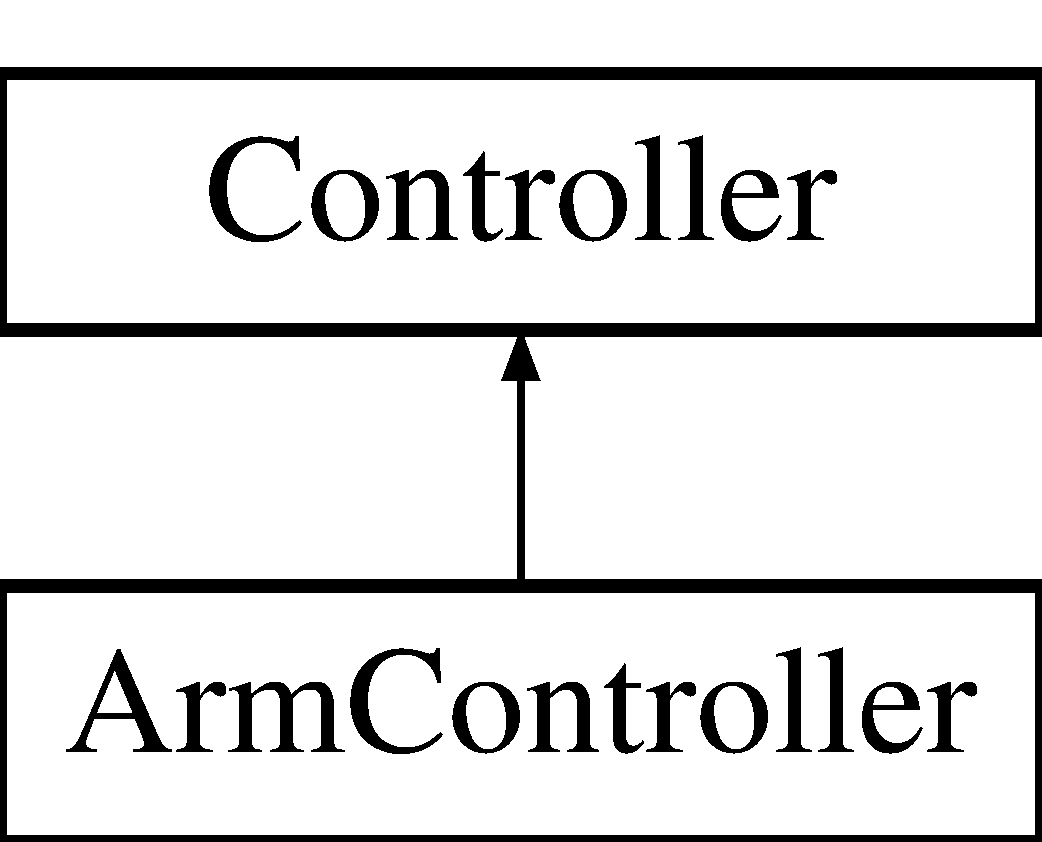
\includegraphics[height=2.000000cm]{classArmController}
\end{center}
\end{figure}
\subsection*{\-Métodos públicos}
\begin{DoxyCompactItemize}
\item 
\hypertarget{classArmController_a9b970431a48ef344677bf4d0c0809fba}{{\bfseries \-Arm\-Controller} (\hyperlink{classdfv_1_1XsensListener}{dfv\-::\-Xsens\-Listener} \&sensors\-\_\-, \hyperlink{classdfv_1_1Youbot}{dfv\-::\-Youbot} \&youbot\-\_\-)}\label{classArmController_a9b970431a48ef344677bf4d0c0809fba}

\item 
\hypertarget{classArmController_a5e4570f96d8dfdfdd4ec029779f15eae}{bool {\bfseries \-On\-Init} ()}\label{classArmController_a5e4570f96d8dfdfdd4ec029779f15eae}

\item 
\hypertarget{classArmController_aa0102892d8753117349d2f406c30c736}{std\-::vector$<$ float $>$ {\bfseries \-On\-Update} ()}\label{classArmController_aa0102892d8753117349d2f406c30c736}

\item 
\hypertarget{classArmController_a210e66d9372edd1f05ba67969aef7d1f}{std\-::vector$<$ float $>$ {\bfseries \-Get\-Angles} ()}\label{classArmController_a210e66d9372edd1f05ba67969aef7d1f}

\end{DoxyCompactItemize}
\subsection*{\-Atributos protegidos}
\begin{DoxyCompactItemize}
\item 
\hypertarget{classArmController_a2c9f1294097ba76e38d820d51809209d}{float {\bfseries ang\-\_\-0\-\_\-offset}}\label{classArmController_a2c9f1294097ba76e38d820d51809209d}

\end{DoxyCompactItemize}


\-La documentación para esta clase fue generada a partir del siguiente fichero\-:\begin{DoxyCompactItemize}
\item 
youbot\-\_\-controller/include/youbot\-\_\-controller/arm\-\_\-controller.\-h\end{DoxyCompactItemize}

\hypertarget{classdfv_1_1Base}{\section{\-Referencia de la \-Clase dfv\-:\-:\-Base}
\label{classdfv_1_1Base}\index{dfv\-::\-Base@{dfv\-::\-Base}}
}
\subsection*{\-Métodos públicos}
\begin{DoxyCompactItemize}
\item 
\hypertarget{classdfv_1_1Base_a2b100a07979db6ab9b7416b220e56ea1}{{\bfseries \-Base} (ros\-::\-Node\-Handle \&\-\_\-node\-\_\-handle)}\label{classdfv_1_1Base_a2b100a07979db6ab9b7416b220e56ea1}

\item 
\hypertarget{classdfv_1_1Base_ad01c3d2429a5c96ec84bc28a2e3383f1}{\hyperlink{classdfv_1_1Base}{\-Base} \& {\bfseries \-Move} (float linear\-\_\-vel, float side\-\_\-vel, float angular\-\_\-vel)}\label{classdfv_1_1Base_ad01c3d2429a5c96ec84bc28a2e3383f1}

\item 
\hypertarget{classdfv_1_1Base_a0b94d4ef402c3dc09cc34e9d8f3ee048}{\hyperlink{classdfv_1_1Base}{\-Base} \& {\bfseries \-Move\-For} (float linear\-\_\-vel, float side\-\_\-vel, float angular\-\_\-vel, float time)}\label{classdfv_1_1Base_a0b94d4ef402c3dc09cc34e9d8f3ee048}

\item 
\hypertarget{classdfv_1_1Base_a7d1dff675ff8f6eeb34d0fa43d2df159}{\hyperlink{classdfv_1_1Base}{\-Base} \& {\bfseries \-Stop} ()}\label{classdfv_1_1Base_a7d1dff675ff8f6eeb34d0fa43d2df159}

\item 
\hypertarget{classdfv_1_1Base_a1a32c5ba00f99819cbdb981089aa7696}{\hyperlink{classdfv_1_1Base}{\-Base} \& {\bfseries \-Enable} ()}\label{classdfv_1_1Base_a1a32c5ba00f99819cbdb981089aa7696}

\item 
\hypertarget{classdfv_1_1Base_a538c9a6798fdf1622d697e0b17f4c8a7}{\hyperlink{classdfv_1_1Base}{\-Base} \& {\bfseries \-Disable} ()}\label{classdfv_1_1Base_a538c9a6798fdf1622d697e0b17f4c8a7}

\end{DoxyCompactItemize}


\-La documentación para esta clase fue generada a partir del siguiente fichero\-:\begin{DoxyCompactItemize}
\item 
dfv/include/dfv/youbot.\-h\end{DoxyCompactItemize}

\hypertarget{classBaseController}{\section{\-Referencia de la \-Clase \-Base\-Controller}
\label{classBaseController}\index{\-Base\-Controller@{\-Base\-Controller}}
}
\-Diagrama de herencias de \-Base\-Controller\begin{figure}[H]
\begin{center}
\leavevmode
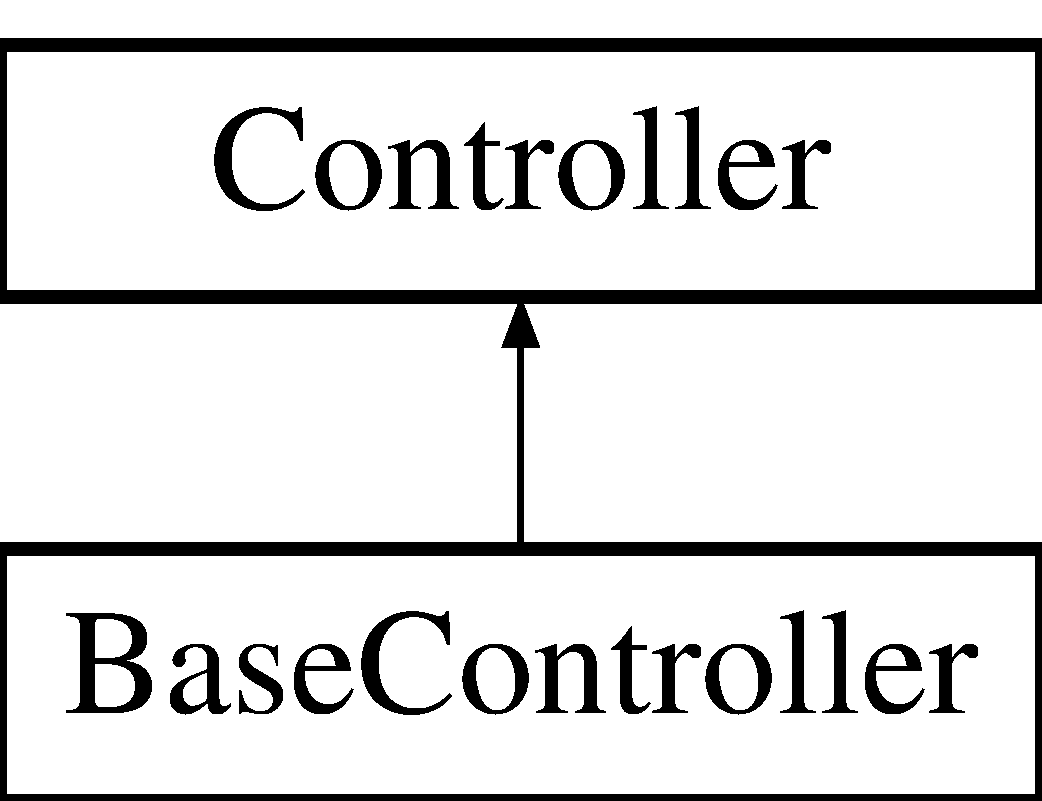
\includegraphics[height=2.000000cm]{classBaseController}
\end{center}
\end{figure}
\subsection*{\-Métodos públicos}
\begin{DoxyCompactItemize}
\item 
\hypertarget{classBaseController_a84dc2838d3a3c571f5f6ec8185f639e3}{{\bfseries \-Base\-Controller} (\hyperlink{classdfv_1_1XsensListener}{dfv\-::\-Xsens\-Listener} \&sensors\-\_\-, \hyperlink{classdfv_1_1Youbot}{dfv\-::\-Youbot} \&youbot\-\_\-)}\label{classBaseController_a84dc2838d3a3c571f5f6ec8185f639e3}

\item 
\hypertarget{classBaseController_a3e7ae02bc05e02b536ddf1975a6770d3}{std\-::vector$<$ float $>$ {\bfseries \-Get\-Vels} ()}\label{classBaseController_a3e7ae02bc05e02b536ddf1975a6770d3}

\item 
\hypertarget{classBaseController_a80f2ea9001a447f023357245d0490488}{virtual std\-::vector$<$ float $>$ {\bfseries \-On\-Update} ()}\label{classBaseController_a80f2ea9001a447f023357245d0490488}

\end{DoxyCompactItemize}


\-La documentación para esta clase fue generada a partir del siguiente fichero\-:\begin{DoxyCompactItemize}
\item 
youbot\-\_\-controller/include/youbot\-\_\-controller/base\-\_\-controller.\-h\end{DoxyCompactItemize}

\hypertarget{classxsens_1_1Cmt1f}{\section{\-Referencia de la \-Clase xsens\-:\-:\-Cmt1f}
\label{classxsens_1_1Cmt1f}\index{xsens\-::\-Cmt1f@{xsens\-::\-Cmt1f}}
}


\-The low-\/level file communication class.  




{\ttfamily \#include $<$cmt1.\-h$>$}

\subsection*{\-Métodos públicos}
\begin{DoxyCompactItemize}
\item 
\hypertarget{classxsens_1_1Cmt1f_a919b42e4de22630c364ce79ff54d8989}{\hyperlink{classxsens_1_1Cmt1f_a919b42e4de22630c364ce79ff54d8989}{\-Cmt1f} ()}\label{classxsens_1_1Cmt1f_a919b42e4de22630c364ce79ff54d8989}

\begin{DoxyCompactList}\small\item\em \-Default constructor, initializes all members to their default values. \end{DoxyCompactList}\item 
\hypertarget{classxsens_1_1Cmt1f_a3f612d9d8c624b8f171a0661ce33ac2a}{\hyperlink{classxsens_1_1Cmt1f_a3f612d9d8c624b8f171a0661ce33ac2a}{$\sim$\-Cmt1f} ()}\label{classxsens_1_1Cmt1f_a3f612d9d8c624b8f171a0661ce33ac2a}

\begin{DoxyCompactList}\small\item\em \-Destructor. \end{DoxyCompactList}\item 
\hyperlink{group__enums_ga822a2260a20af524029eef9e9a51ff6f}{\-Xsens\-Result\-Value} \hyperlink{classxsens_1_1Cmt1f_a761759c365acf23f7e4159b5bedb1ae4}{append\-Data} (const uint32\-\_\-t length, const void $\ast$data)
\begin{DoxyCompactList}\small\item\em \-Write data to the end of the file. \end{DoxyCompactList}\item 
\hypertarget{classxsens_1_1Cmt1f_a998f005fb3832d4945e53a41b570d634}{\hyperlink{group__enums_ga822a2260a20af524029eef9e9a51ff6f}{\-Xsens\-Result\-Value} \hyperlink{classxsens_1_1Cmt1f_a998f005fb3832d4945e53a41b570d634}{close} (void)}\label{classxsens_1_1Cmt1f_a998f005fb3832d4945e53a41b570d634}

\begin{DoxyCompactList}\small\item\em \-Close the file. \end{DoxyCompactList}\item 
\hypertarget{classxsens_1_1Cmt1f_a7f88bf518daead18acd478c53874f59e}{\hyperlink{group__enums_ga822a2260a20af524029eef9e9a51ff6f}{\-Xsens\-Result\-Value} \hyperlink{classxsens_1_1Cmt1f_a7f88bf518daead18acd478c53874f59e}{close\-And\-Delete} (void)}\label{classxsens_1_1Cmt1f_a7f88bf518daead18acd478c53874f59e}

\begin{DoxyCompactList}\small\item\em \-Close the file and delete it. \end{DoxyCompactList}\item 
\hypertarget{classxsens_1_1Cmt1f_afe9e7fd93967527fcabfdc0e248f9acc}{\hyperlink{group__enums_ga822a2260a20af524029eef9e9a51ff6f}{\-Xsens\-Result\-Value} \hyperlink{classxsens_1_1Cmt1f_afe9e7fd93967527fcabfdc0e248f9acc}{create} (const char $\ast$filename)}\label{classxsens_1_1Cmt1f_afe9e7fd93967527fcabfdc0e248f9acc}

\begin{DoxyCompactList}\small\item\em \-Open an empty file. \end{DoxyCompactList}\item 
\hypertarget{classxsens_1_1Cmt1f_ae45a131665d3f94c209d51bdb382425c}{\hyperlink{group__enums_ga822a2260a20af524029eef9e9a51ff6f}{\-Xsens\-Result\-Value} \hyperlink{classxsens_1_1Cmt1f_ae45a131665d3f94c209d51bdb382425c}{create} (const wchar\-\_\-t $\ast$filename)}\label{classxsens_1_1Cmt1f_ae45a131665d3f94c209d51bdb382425c}

\begin{DoxyCompactList}\small\item\em \-Open an empty file using a unicode path + filename. \end{DoxyCompactList}\item 
\hyperlink{group__enums_ga822a2260a20af524029eef9e9a51ff6f}{\-Xsens\-Result\-Value} \hyperlink{classxsens_1_1Cmt1f_a51f143e00f87b2cfab723654bac58ec1}{delete\-Data} (const \-Xsens\-File\-Pos start, const uint32\-\_\-t length)
\begin{DoxyCompactList}\small\item\em \-Delete the given data from the file. \end{DoxyCompactList}\item 
\hyperlink{group__enums_ga822a2260a20af524029eef9e9a51ff6f}{\-Xsens\-Result\-Value} \hyperlink{classxsens_1_1Cmt1f_a0ddcd0eb51efc0a53348b8cdb2d82d7a}{find} (const void $\ast$needle, const uint32\-\_\-t needle\-Length, \-Xsens\-File\-Pos \&pos)
\begin{DoxyCompactList}\small\item\em \-Find a string of bytes in the file. \end{DoxyCompactList}\item 
\hypertarget{classxsens_1_1Cmt1f_aebb4f05e2a6b0006da18fd7b21443a89}{\hyperlink{group__enums_ga822a2260a20af524029eef9e9a51ff6f}{\-Xsens\-Result\-Value} \hyperlink{classxsens_1_1Cmt1f_aebb4f05e2a6b0006da18fd7b21443a89}{flush\-Data} (void)}\label{classxsens_1_1Cmt1f_aebb4f05e2a6b0006da18fd7b21443a89}

\begin{DoxyCompactList}\small\item\em \-Flush all data to be written. \-This function writes any remaining data immediately and does not return until this is done. \end{DoxyCompactList}\item 
\hypertarget{classxsens_1_1Cmt1f_af4b0d90ae27736caa5f9b9c848c7e08b}{\-Xsens\-File\-Pos \hyperlink{classxsens_1_1Cmt1f_af4b0d90ae27736caa5f9b9c848c7e08b}{get\-File\-Size} (void) const }\label{classxsens_1_1Cmt1f_af4b0d90ae27736caa5f9b9c848c7e08b}

\begin{DoxyCompactList}\small\item\em \-Return the size of the file. \end{DoxyCompactList}\item 
\hypertarget{classxsens_1_1Cmt1f_ac1177c0bb97bdeacac9ccc21d3f8646d}{\hyperlink{group__enums_ga822a2260a20af524029eef9e9a51ff6f}{\-Xsens\-Result\-Value} \hyperlink{classxsens_1_1Cmt1f_ac1177c0bb97bdeacac9ccc21d3f8646d}{get\-Last\-Result} (void) const }\label{classxsens_1_1Cmt1f_ac1177c0bb97bdeacac9ccc21d3f8646d}

\begin{DoxyCompactList}\small\item\em \-Return the result code of the last operation. \end{DoxyCompactList}\item 
\hyperlink{group__enums_ga822a2260a20af524029eef9e9a51ff6f}{\-Xsens\-Result\-Value} \hyperlink{classxsens_1_1Cmt1f_a1447858cb01e173d8ee02f45e39a39f2}{get\-Name} (char $\ast$filename) const 
\begin{DoxyCompactList}\small\item\em \-Retrieve the filename that was last successfully opened. \end{DoxyCompactList}\item 
\hyperlink{group__enums_ga822a2260a20af524029eef9e9a51ff6f}{\-Xsens\-Result\-Value} \hyperlink{classxsens_1_1Cmt1f_a6cf9e6b889f186c2d2e41c877f01831e}{get\-Name} (wchar\-\_\-t $\ast$filename) const 
\begin{DoxyCompactList}\small\item\em \-Retrieve the filename that was last successfully opened in unicode. \end{DoxyCompactList}\item 
\hypertarget{classxsens_1_1Cmt1f_a50dd342eb0ff14be0439b20aaaa328e1}{\-Xsens\-File\-Pos \hyperlink{classxsens_1_1Cmt1f_a50dd342eb0ff14be0439b20aaaa328e1}{get\-Read\-Pos} (void) const }\label{classxsens_1_1Cmt1f_a50dd342eb0ff14be0439b20aaaa328e1}

\begin{DoxyCompactList}\small\item\em \-Return the current read position. \end{DoxyCompactList}\item 
\hypertarget{classxsens_1_1Cmt1f_a23d703467b142bddd066748489924e08}{\-Xsens\-File\-Pos \hyperlink{classxsens_1_1Cmt1f_a23d703467b142bddd066748489924e08}{get\-Write\-Pos} (void) const }\label{classxsens_1_1Cmt1f_a23d703467b142bddd066748489924e08}

\begin{DoxyCompactList}\small\item\em \-Return the current write position. \end{DoxyCompactList}\item 
\hyperlink{group__enums_ga822a2260a20af524029eef9e9a51ff6f}{\-Xsens\-Result\-Value} \hyperlink{classxsens_1_1Cmt1f_a7aaf400038c7dc83120eb0c166aa789d}{insert\-Data} (const \-Xsens\-File\-Pos start, const uint32\-\_\-t length, const void $\ast$data)
\begin{DoxyCompactList}\small\item\em \-Insert the given data into the file. \end{DoxyCompactList}\item 
\hypertarget{classxsens_1_1Cmt1f_a2068defb2740556214948f20b23e602c}{bool \hyperlink{classxsens_1_1Cmt1f_a2068defb2740556214948f20b23e602c}{is\-Open} (void) const }\label{classxsens_1_1Cmt1f_a2068defb2740556214948f20b23e602c}

\begin{DoxyCompactList}\small\item\em \-Return whether the file is open or not. \end{DoxyCompactList}\item 
\hypertarget{classxsens_1_1Cmt1f_a176ec162dda5146c4f91024eb4fd1778}{bool \hyperlink{classxsens_1_1Cmt1f_a176ec162dda5146c4f91024eb4fd1778}{is\-Read\-Only} (void) const }\label{classxsens_1_1Cmt1f_a176ec162dda5146c4f91024eb4fd1778}

\begin{DoxyCompactList}\small\item\em \-Return whether the file is readonly or not. \end{DoxyCompactList}\item 
\hypertarget{classxsens_1_1Cmt1f_ac3623b1bd3ab4aa7aaa1cdfe494494d7}{\hyperlink{group__enums_ga822a2260a20af524029eef9e9a51ff6f}{\-Xsens\-Result\-Value} \hyperlink{classxsens_1_1Cmt1f_ac3623b1bd3ab4aa7aaa1cdfe494494d7}{open} (const char $\ast$filename, const bool \hyperlink{classxsens_1_1Cmt1f_afe9e7fd93967527fcabfdc0e248f9acc}{create}, const bool read\-Only)}\label{classxsens_1_1Cmt1f_ac3623b1bd3ab4aa7aaa1cdfe494494d7}

\begin{DoxyCompactList}\small\item\em \-Open a file. \end{DoxyCompactList}\item 
\hypertarget{classxsens_1_1Cmt1f_a32a7d14f2a28e4624e00168c16c5e5c5}{\hyperlink{group__enums_ga822a2260a20af524029eef9e9a51ff6f}{\-Xsens\-Result\-Value} \hyperlink{classxsens_1_1Cmt1f_a32a7d14f2a28e4624e00168c16c5e5c5}{open} (const wchar\-\_\-t $\ast$filename, const bool \hyperlink{classxsens_1_1Cmt1f_afe9e7fd93967527fcabfdc0e248f9acc}{create}, const bool read\-Only)}\label{classxsens_1_1Cmt1f_a32a7d14f2a28e4624e00168c16c5e5c5}

\begin{DoxyCompactList}\small\item\em \-Open a file using a unicode filename. \end{DoxyCompactList}\item 
\hyperlink{group__enums_ga822a2260a20af524029eef9e9a51ff6f}{\-Xsens\-Result\-Value} \hyperlink{classxsens_1_1Cmt1f_ad5850430ffa0988986c0b10d218023a2}{read\-Data} (const uint32\-\_\-t max\-Length, void $\ast$data, uint32\-\_\-t $\ast$length)
\begin{DoxyCompactList}\small\item\em \-Read data from the file and put it into the data buffer. \end{DoxyCompactList}\item 
\hyperlink{group__enums_ga822a2260a20af524029eef9e9a51ff6f}{\-Xsens\-Result\-Value} \hyperlink{classxsens_1_1Cmt1f_ad264a2ef6cdc9a6cfe0b9fce04e466f0}{read\-Data} (const uint32\-\_\-t max\-Length, const char terminator, void $\ast$data, uint32\-\_\-t $\ast$length)
\begin{DoxyCompactList}\small\item\em \-Read data from the file and put it into the data buffer. \end{DoxyCompactList}\item 
\hyperlink{group__enums_ga822a2260a20af524029eef9e9a51ff6f}{\-Xsens\-Result\-Value} \hyperlink{classxsens_1_1Cmt1f_ae901294366012d032ebe13660a1564cc}{set\-Read\-Pos} (const \-Xsens\-File\-Pos pos)
\begin{DoxyCompactList}\small\item\em \-Set the new absolute read position. \end{DoxyCompactList}\item 
\hyperlink{group__enums_ga822a2260a20af524029eef9e9a51ff6f}{\-Xsens\-Result\-Value} \hyperlink{classxsens_1_1Cmt1f_a783c34b3976303be5e776c6b0d815768}{set\-Write\-Pos} (const \-Xsens\-File\-Pos pos=-\/1)
\begin{DoxyCompactList}\small\item\em \-Set the new absolute write position. \end{DoxyCompactList}\item 
\hyperlink{group__enums_ga822a2260a20af524029eef9e9a51ff6f}{\-Xsens\-Result\-Value} \hyperlink{classxsens_1_1Cmt1f_aa62d96ccce3c8e407d20bd0346d94991}{write\-Data} (const uint32\-\_\-t length, const void $\ast$data)
\begin{DoxyCompactList}\small\item\em \-Write data to the file. \end{DoxyCompactList}\end{DoxyCompactItemize}
\subsection*{\-Métodos protegidos}
\begin{DoxyCompactItemize}
\item 
\hypertarget{classxsens_1_1Cmt1f_a06211472647b5865767127ce404713bf}{void \hyperlink{classxsens_1_1Cmt1f_a06211472647b5865767127ce404713bf}{goto\-Read} (void)}\label{classxsens_1_1Cmt1f_a06211472647b5865767127ce404713bf}

\begin{DoxyCompactList}\small\item\em \-Change from writing to reading mode. \end{DoxyCompactList}\item 
\hypertarget{classxsens_1_1Cmt1f_a70655b6aa0207f32b9bb89e0bfbeda07}{void \hyperlink{classxsens_1_1Cmt1f_a70655b6aa0207f32b9bb89e0bfbeda07}{goto\-Write} (void)}\label{classxsens_1_1Cmt1f_a70655b6aa0207f32b9bb89e0bfbeda07}

\begin{DoxyCompactList}\small\item\em \-Change from reading to writing mode. \end{DoxyCompactList}\end{DoxyCompactItemize}
\subsection*{\-Atributos protegidos}
\begin{DoxyCompactItemize}
\item 
\hypertarget{classxsens_1_1Cmt1f_a9e626704be273497ae4e1408a4aa3b7b}{\-F\-I\-L\-E $\ast$ \hyperlink{classxsens_1_1Cmt1f_a9e626704be273497ae4e1408a4aa3b7b}{m\-\_\-handle}}\label{classxsens_1_1Cmt1f_a9e626704be273497ae4e1408a4aa3b7b}

\begin{DoxyCompactList}\small\item\em \-The file handle. \end{DoxyCompactList}\item 
\hypertarget{classxsens_1_1Cmt1f_a3e3ea40ffe4c4b4d49a18bfe70c52171}{\-Xsens\-File\-Pos \hyperlink{classxsens_1_1Cmt1f_a3e3ea40ffe4c4b4d49a18bfe70c52171}{m\-\_\-file\-Size}}\label{classxsens_1_1Cmt1f_a3e3ea40ffe4c4b4d49a18bfe70c52171}

\begin{DoxyCompactList}\small\item\em \-Contains the size of the file. \end{DoxyCompactList}\item 
\hypertarget{classxsens_1_1Cmt1f_a8a3470f287b0483a35ad990fa654273a}{\-Xsens\-File\-Pos \hyperlink{classxsens_1_1Cmt1f_a8a3470f287b0483a35ad990fa654273a}{m\-\_\-read\-Pos}}\label{classxsens_1_1Cmt1f_a8a3470f287b0483a35ad990fa654273a}

\begin{DoxyCompactList}\small\item\em \-The last read position in the file. \end{DoxyCompactList}\item 
\hypertarget{classxsens_1_1Cmt1f_a29a6e0711c381ba77bac31453c3fca2c}{\-Xsens\-File\-Pos \hyperlink{classxsens_1_1Cmt1f_a29a6e0711c381ba77bac31453c3fca2c}{m\-\_\-write\-Pos}}\label{classxsens_1_1Cmt1f_a29a6e0711c381ba77bac31453c3fca2c}

\begin{DoxyCompactList}\small\item\em \-The last write position in the file. \end{DoxyCompactList}\item 
\hypertarget{classxsens_1_1Cmt1f_a986315e350d8c3c8aed0526e77bd4ed9}{\hyperlink{group__enums_ga822a2260a20af524029eef9e9a51ff6f}{\-Xsens\-Result\-Value} \hyperlink{classxsens_1_1Cmt1f_a986315e350d8c3c8aed0526e77bd4ed9}{m\-\_\-last\-Result}}\label{classxsens_1_1Cmt1f_a986315e350d8c3c8aed0526e77bd4ed9}

\begin{DoxyCompactList}\small\item\em \-The last result of an operation. \end{DoxyCompactList}\item 
\hypertarget{classxsens_1_1Cmt1f_a43ddc4718e69ed4fe21c6574da58f4d2}{char \hyperlink{classxsens_1_1Cmt1f_a43ddc4718e69ed4fe21c6574da58f4d2}{m\-\_\-filename} \mbox{[}\-C\-M\-T\-\_\-\-M\-A\-X\-\_\-\-F\-I\-L\-E\-N\-A\-M\-E\-\_\-\-L\-E\-N\-G\-T\-H\mbox{]}}\label{classxsens_1_1Cmt1f_a43ddc4718e69ed4fe21c6574da58f4d2}

\begin{DoxyCompactList}\small\item\em \-Contains the name of the file that was last successfully opened. \end{DoxyCompactList}\item 
\hypertarget{classxsens_1_1Cmt1f_a794d7d18b2ea76cf8a6455072261f6b9}{wchar\-\_\-t \hyperlink{classxsens_1_1Cmt1f_a794d7d18b2ea76cf8a6455072261f6b9}{m\-\_\-filename\-\_\-w} \mbox{[}\-C\-M\-T\-\_\-\-M\-A\-X\-\_\-\-F\-I\-L\-E\-N\-A\-M\-E\-\_\-\-L\-E\-N\-G\-T\-H\mbox{]}}\label{classxsens_1_1Cmt1f_a794d7d18b2ea76cf8a6455072261f6b9}

\begin{DoxyCompactList}\small\item\em \-Contains the name of the file that was last successfully opened using unicode. \end{DoxyCompactList}\item 
\hypertarget{classxsens_1_1Cmt1f_a5f2130dc8026b6a8ad55ffbdaac74150}{bool \hyperlink{classxsens_1_1Cmt1f_a5f2130dc8026b6a8ad55ffbdaac74150}{m\-\_\-is\-Open}}\label{classxsens_1_1Cmt1f_a5f2130dc8026b6a8ad55ffbdaac74150}

\begin{DoxyCompactList}\small\item\em \-Indicates if the file is open or not. \end{DoxyCompactList}\item 
\hypertarget{classxsens_1_1Cmt1f_a6da996485f79b6aa12b089b31dc4c654}{bool \hyperlink{classxsens_1_1Cmt1f_a6da996485f79b6aa12b089b31dc4c654}{m\-\_\-unicode}}\label{classxsens_1_1Cmt1f_a6da996485f79b6aa12b089b31dc4c654}

\begin{DoxyCompactList}\small\item\em \-Indicates if we're using the unicode filename or the regular filename. \end{DoxyCompactList}\item 
bool \hyperlink{classxsens_1_1Cmt1f_a743b759eb55ae888d44a37c865870bb4}{m\-\_\-reading}
\begin{DoxyCompactList}\small\item\em \-Indicates whether the last operation was a read or write operation. \end{DoxyCompactList}\item 
\hypertarget{classxsens_1_1Cmt1f_ac87b9035d8cbd6d3f7ecff38660a4216}{bool \hyperlink{classxsens_1_1Cmt1f_ac87b9035d8cbd6d3f7ecff38660a4216}{m\-\_\-read\-Only}}\label{classxsens_1_1Cmt1f_ac87b9035d8cbd6d3f7ecff38660a4216}

\begin{DoxyCompactList}\small\item\em \-Indicates if the file was opened in read-\/only mode. \end{DoxyCompactList}\end{DoxyCompactItemize}


\subsection{\-Descripción detallada}
\-The low-\/level file communication class. 

\subsection{\-Documentación de las funciones miembro}
\hypertarget{classxsens_1_1Cmt1f_a761759c365acf23f7e4159b5bedb1ae4}{\index{xsens\-::\-Cmt1f@{xsens\-::\-Cmt1f}!append\-Data@{append\-Data}}
\index{append\-Data@{append\-Data}!xsens::Cmt1f@{xsens\-::\-Cmt1f}}
\subsubsection[{append\-Data}]{\setlength{\rightskip}{0pt plus 5cm}{\bf \-Xsens\-Result\-Value} {\bf xsens\-::\-Cmt1f\-::append\-Data} (
\begin{DoxyParamCaption}
\item[{const uint32\-\_\-t}]{length, }
\item[{const void $\ast$}]{data}
\end{DoxyParamCaption}
)}}\label{classxsens_1_1Cmt1f_a761759c365acf23f7e4159b5bedb1ae4}


\-Write data to the end of the file. 

\-The function writes the given data to the file at the end. \-The current write position is also moved to the end of the file. \hypertarget{classxsens_1_1Cmt1f_a51f143e00f87b2cfab723654bac58ec1}{\index{xsens\-::\-Cmt1f@{xsens\-::\-Cmt1f}!delete\-Data@{delete\-Data}}
\index{delete\-Data@{delete\-Data}!xsens::Cmt1f@{xsens\-::\-Cmt1f}}
\subsubsection[{delete\-Data}]{\setlength{\rightskip}{0pt plus 5cm}{\bf \-Xsens\-Result\-Value} {\bf xsens\-::\-Cmt1f\-::delete\-Data} (
\begin{DoxyParamCaption}
\item[{const \-Xsens\-File\-Pos}]{start, }
\item[{const uint32\-\_\-t}]{length}
\end{DoxyParamCaption}
)}}\label{classxsens_1_1Cmt1f_a51f143e00f87b2cfab723654bac58ec1}


\-Delete the given data from the file. 

\-The function erases the given data from the file at the given write position. \-This operation may take a while to complete, but is faster than insert\-Data.

\-The write position is not changed and the read position is checked for validity. \hypertarget{classxsens_1_1Cmt1f_a0ddcd0eb51efc0a53348b8cdb2d82d7a}{\index{xsens\-::\-Cmt1f@{xsens\-::\-Cmt1f}!find@{find}}
\index{find@{find}!xsens::Cmt1f@{xsens\-::\-Cmt1f}}
\subsubsection[{find}]{\setlength{\rightskip}{0pt plus 5cm}{\bf \-Xsens\-Result\-Value} {\bf xsens\-::\-Cmt1f\-::find} (
\begin{DoxyParamCaption}
\item[{const void $\ast$}]{needle, }
\item[{const uint32\-\_\-t}]{needle\-Length, }
\item[{\-Xsens\-File\-Pos \&}]{pos}
\end{DoxyParamCaption}
)}}\label{classxsens_1_1Cmt1f_a0ddcd0eb51efc0a53348b8cdb2d82d7a}


\-Find a string of bytes in the file. 

\-The function searches from the current read position until the given {\ttfamily needle} is found. \-If the needle is not found, \-Xsens\-Result\-Value\-::\-N\-O\-T\-\_\-\-F\-O\-U\-N\-D is returned. \-The function will update the seek position to the first character of the found needle. 
\begin{DoxyParams}{\-Parámetros}
{\em needle} & \-The byte string to find. \\
\hline
{\em needle\-Length} & \-The length of the byte string. \\
\hline
{\em pos} & \-Out\-: \-The position where the needle was found. \-This will point to the first character of the found needle. \\
\hline
\end{DoxyParams}
\hypertarget{classxsens_1_1Cmt1f_a1447858cb01e173d8ee02f45e39a39f2}{\index{xsens\-::\-Cmt1f@{xsens\-::\-Cmt1f}!get\-Name@{get\-Name}}
\index{get\-Name@{get\-Name}!xsens::Cmt1f@{xsens\-::\-Cmt1f}}
\subsubsection[{get\-Name}]{\setlength{\rightskip}{0pt plus 5cm}{\bf \-Xsens\-Result\-Value} {\bf xsens\-::\-Cmt1f\-::get\-Name} (
\begin{DoxyParamCaption}
\item[{char $\ast$}]{filename}
\end{DoxyParamCaption}
) const}}\label{classxsens_1_1Cmt1f_a1447858cb01e173d8ee02f45e39a39f2}


\-Retrieve the filename that was last successfully opened. 


\begin{DoxyParams}{\-Parámetros}
{\em filename} & \-A buffer for storing the filename. \-The buffer should be able to hold the filename. \-A safe size is to make it at least 256 bytes. \\
\hline
\end{DoxyParams}
\hypertarget{classxsens_1_1Cmt1f_a6cf9e6b889f186c2d2e41c877f01831e}{\index{xsens\-::\-Cmt1f@{xsens\-::\-Cmt1f}!get\-Name@{get\-Name}}
\index{get\-Name@{get\-Name}!xsens::Cmt1f@{xsens\-::\-Cmt1f}}
\subsubsection[{get\-Name}]{\setlength{\rightskip}{0pt plus 5cm}{\bf \-Xsens\-Result\-Value} {\bf xsens\-::\-Cmt1f\-::get\-Name} (
\begin{DoxyParamCaption}
\item[{wchar\-\_\-t $\ast$}]{filename}
\end{DoxyParamCaption}
) const}}\label{classxsens_1_1Cmt1f_a6cf9e6b889f186c2d2e41c877f01831e}


\-Retrieve the filename that was last successfully opened in unicode. 


\begin{DoxyParams}{\-Parámetros}
{\em filename} & \-A buffer for storing the filename. \-The buffer should be able to hold the filename. \-A safe size is to make it at least 256 wide characters. \\
\hline
\end{DoxyParams}
\hypertarget{classxsens_1_1Cmt1f_a7aaf400038c7dc83120eb0c166aa789d}{\index{xsens\-::\-Cmt1f@{xsens\-::\-Cmt1f}!insert\-Data@{insert\-Data}}
\index{insert\-Data@{insert\-Data}!xsens::Cmt1f@{xsens\-::\-Cmt1f}}
\subsubsection[{insert\-Data}]{\setlength{\rightskip}{0pt plus 5cm}{\bf \-Xsens\-Result\-Value} {\bf xsens\-::\-Cmt1f\-::insert\-Data} (
\begin{DoxyParamCaption}
\item[{const \-Xsens\-File\-Pos}]{start, }
\item[{const uint32\-\_\-t}]{length, }
\item[{const void $\ast$}]{data}
\end{DoxyParamCaption}
)}}\label{classxsens_1_1Cmt1f_a7aaf400038c7dc83120eb0c166aa789d}


\-Insert the given data into the file. 

\-The function writes the given data to the file at the current write position. \-This operation may take a while to complete.

\-The write position is placed at the end of the inserted data. \hypertarget{classxsens_1_1Cmt1f_ad5850430ffa0988986c0b10d218023a2}{\index{xsens\-::\-Cmt1f@{xsens\-::\-Cmt1f}!read\-Data@{read\-Data}}
\index{read\-Data@{read\-Data}!xsens::Cmt1f@{xsens\-::\-Cmt1f}}
\subsubsection[{read\-Data}]{\setlength{\rightskip}{0pt plus 5cm}{\bf \-Xsens\-Result\-Value} {\bf xsens\-::\-Cmt1f\-::read\-Data} (
\begin{DoxyParamCaption}
\item[{const uint32\-\_\-t}]{max\-Length, }
\item[{void $\ast$}]{data, }
\item[{uint32\-\_\-t $\ast$}]{length}
\end{DoxyParamCaption}
)}}\label{classxsens_1_1Cmt1f_ad5850430ffa0988986c0b10d218023a2}


\-Read data from the file and put it into the data buffer. 

\-This function reads exactly the number of bytes as requested from the file. 
\begin{DoxyParams}{\-Parámetros}
{\em max\-Length} & \-The amount of data that will be read. \\
\hline
{\em data} & \-Pointer to a buffer that will store the read data. \\
\hline
{\em length} & pointer to a variable that will store the number of bytes that were actually read. \-The parameter may be \-N\-U\-L\-L. \\
\hline
\end{DoxyParams}
\hypertarget{classxsens_1_1Cmt1f_ad264a2ef6cdc9a6cfe0b9fce04e466f0}{\index{xsens\-::\-Cmt1f@{xsens\-::\-Cmt1f}!read\-Data@{read\-Data}}
\index{read\-Data@{read\-Data}!xsens::Cmt1f@{xsens\-::\-Cmt1f}}
\subsubsection[{read\-Data}]{\setlength{\rightskip}{0pt plus 5cm}{\bf \-Xsens\-Result\-Value} {\bf xsens\-::\-Cmt1f\-::read\-Data} (
\begin{DoxyParamCaption}
\item[{const uint32\-\_\-t}]{max\-Length, }
\item[{const char}]{terminator, }
\item[{void $\ast$}]{data, }
\item[{uint32\-\_\-t $\ast$}]{length}
\end{DoxyParamCaption}
)}}\label{classxsens_1_1Cmt1f_ad264a2ef6cdc9a6cfe0b9fce04e466f0}


\-Read data from the file and put it into the data buffer. 

\-This function reads upp to the number of bytes as requested from the file. \-The function will also stop if the given terminator character is encountered. \-The terminator is included in the output buffer. 
\begin{DoxyParams}{\-Parámetros}
{\em max\-Length} & \-The amount of data that will be read. \\
\hline
{\em data} & \-Pointer to a buffer that will store the read data. \\
\hline
{\em terminator} & \-A character that will end the read operation if encountered. \\
\hline
{\em length} & \-The actual number of bytes read, including the terminator character, if encountered. \\
\hline
\end{DoxyParams}
\hypertarget{classxsens_1_1Cmt1f_ae901294366012d032ebe13660a1564cc}{\index{xsens\-::\-Cmt1f@{xsens\-::\-Cmt1f}!set\-Read\-Pos@{set\-Read\-Pos}}
\index{set\-Read\-Pos@{set\-Read\-Pos}!xsens::Cmt1f@{xsens\-::\-Cmt1f}}
\subsubsection[{set\-Read\-Pos}]{\setlength{\rightskip}{0pt plus 5cm}{\bf \-Xsens\-Result\-Value} {\bf xsens\-::\-Cmt1f\-::set\-Read\-Pos} (
\begin{DoxyParamCaption}
\item[{const \-Xsens\-File\-Pos}]{pos}
\end{DoxyParamCaption}
)}}\label{classxsens_1_1Cmt1f_ae901294366012d032ebe13660a1564cc}


\-Set the new absolute read position. 

\-The read position is checked against the filesize before committing. \hypertarget{classxsens_1_1Cmt1f_a783c34b3976303be5e776c6b0d815768}{\index{xsens\-::\-Cmt1f@{xsens\-::\-Cmt1f}!set\-Write\-Pos@{set\-Write\-Pos}}
\index{set\-Write\-Pos@{set\-Write\-Pos}!xsens::Cmt1f@{xsens\-::\-Cmt1f}}
\subsubsection[{set\-Write\-Pos}]{\setlength{\rightskip}{0pt plus 5cm}{\bf \-Xsens\-Result\-Value} {\bf xsens\-::\-Cmt1f\-::set\-Write\-Pos} (
\begin{DoxyParamCaption}
\item[{const \-Xsens\-File\-Pos}]{pos = {\ttfamily -\/1}}
\end{DoxyParamCaption}
)}}\label{classxsens_1_1Cmt1f_a783c34b3976303be5e776c6b0d815768}


\-Set the new absolute write position. 

\-The write position is checked against the filesize before committing. \hypertarget{classxsens_1_1Cmt1f_aa62d96ccce3c8e407d20bd0346d94991}{\index{xsens\-::\-Cmt1f@{xsens\-::\-Cmt1f}!write\-Data@{write\-Data}}
\index{write\-Data@{write\-Data}!xsens::Cmt1f@{xsens\-::\-Cmt1f}}
\subsubsection[{write\-Data}]{\setlength{\rightskip}{0pt plus 5cm}{\bf \-Xsens\-Result\-Value} {\bf xsens\-::\-Cmt1f\-::write\-Data} (
\begin{DoxyParamCaption}
\item[{const uint32\-\_\-t}]{length, }
\item[{const void $\ast$}]{data}
\end{DoxyParamCaption}
)}}\label{classxsens_1_1Cmt1f_aa62d96ccce3c8e407d20bd0346d94991}


\-Write data to the file. 

\-The function writes the given data to the file at the current write position. 

\subsection{\-Documentación de los datos miembro}
\hypertarget{classxsens_1_1Cmt1f_a743b759eb55ae888d44a37c865870bb4}{\index{xsens\-::\-Cmt1f@{xsens\-::\-Cmt1f}!m\-\_\-reading@{m\-\_\-reading}}
\index{m\-\_\-reading@{m\-\_\-reading}!xsens::Cmt1f@{xsens\-::\-Cmt1f}}
\subsubsection[{m\-\_\-reading}]{\setlength{\rightskip}{0pt plus 5cm}bool {\bf xsens\-::\-Cmt1f\-::m\-\_\-reading}\hspace{0.3cm}{\ttfamily  \mbox{[}protected\mbox{]}}}}\label{classxsens_1_1Cmt1f_a743b759eb55ae888d44a37c865870bb4}


\-Indicates whether the last operation was a read or write operation. 

\-This value is used to check whether or not a seek is required to perform a requested read or write operation. 

\-La documentación para esta clase fue generada a partir del siguiente fichero\-:\begin{DoxyCompactItemize}
\item 
xsens\-\_\-driver/include/xsens\-\_\-driver/\hyperlink{cmt1_8h}{cmt1.\-h}\end{DoxyCompactItemize}

\hypertarget{classxsens_1_1Cmt1s}{\section{\-Referencia de la \-Clase xsens\-:\-:\-Cmt1s}
\label{classxsens_1_1Cmt1s}\index{xsens\-::\-Cmt1s@{xsens\-::\-Cmt1s}}
}


\-The low-\/level serial communication class.  




{\ttfamily \#include $<$cmt1.\-h$>$}

\subsection*{\-Métodos públicos}
\begin{DoxyCompactItemize}
\item 
\hypertarget{classxsens_1_1Cmt1s_a04d25a1665542ca7fa840db99fd91a07}{\hyperlink{classxsens_1_1Cmt1s_a04d25a1665542ca7fa840db99fd91a07}{\-Cmt1s} ()}\label{classxsens_1_1Cmt1s_a04d25a1665542ca7fa840db99fd91a07}

\begin{DoxyCompactList}\small\item\em \-Default constructor, initializes all members to their default values. \end{DoxyCompactList}\item 
\hypertarget{classxsens_1_1Cmt1s_acb907ca4246dc9b76f38dfdf46a2d212}{\hyperlink{classxsens_1_1Cmt1s_acb907ca4246dc9b76f38dfdf46a2d212}{$\sim$\-Cmt1s} ()}\label{classxsens_1_1Cmt1s_acb907ca4246dc9b76f38dfdf46a2d212}

\begin{DoxyCompactList}\small\item\em \-Destructor, de-\/initializes, frees memory allocated for buffers, etc. \end{DoxyCompactList}\item 
\hypertarget{classxsens_1_1Cmt1s_a29d64fe8e43430225b02450cac4a65eb}{\hyperlink{group__enums_ga822a2260a20af524029eef9e9a51ff6f}{\-Xsens\-Result\-Value} \hyperlink{classxsens_1_1Cmt1s_a29d64fe8e43430225b02450cac4a65eb}{close} (void)}\label{classxsens_1_1Cmt1s_a29d64fe8e43430225b02450cac4a65eb}

\begin{DoxyCompactList}\small\item\em \-Close the serial communication port. \end{DoxyCompactList}\item 
\hyperlink{group__enums_ga822a2260a20af524029eef9e9a51ff6f}{\-Xsens\-Result\-Value} \hyperlink{classxsens_1_1Cmt1s_a59ea4755515aee0d93c76fd1298388f0}{escape} (const \-Cmt\-Control\-Line mask, const \-Cmt\-Control\-Line state)
\begin{DoxyCompactList}\small\item\em \-Manipulate the \-Serial control lines. \end{DoxyCompactList}\item 
\hyperlink{group__enums_ga822a2260a20af524029eef9e9a51ff6f}{\-Xsens\-Result\-Value} \hyperlink{classxsens_1_1Cmt1s_a99c68d96454c25926a8c21fe0f47538c}{flush\-Data} (void)
\begin{DoxyCompactList}\small\item\em \-Flush all data to be transmitted / received. \end{DoxyCompactList}\item 
\hypertarget{classxsens_1_1Cmt1s_a2fa3c6574b80034820b837536ad04ceb}{uint32\-\_\-t \hyperlink{classxsens_1_1Cmt1s_a2fa3c6574b80034820b837536ad04ceb}{get\-Baudrate} (void) const }\label{classxsens_1_1Cmt1s_a2fa3c6574b80034820b837536ad04ceb}

\begin{DoxyCompactList}\small\item\em \-Return the baudrate that is currently being used by the port. \end{DoxyCompactList}\item 
\hypertarget{classxsens_1_1Cmt1s_aaecc76cad90f7d0bef178d978f02784e}{\-H\-A\-N\-D\-L\-E \hyperlink{classxsens_1_1Cmt1s_aaecc76cad90f7d0bef178d978f02784e}{get\-Handle} (void) const }\label{classxsens_1_1Cmt1s_aaecc76cad90f7d0bef178d978f02784e}

\begin{DoxyCompactList}\small\item\em \-Return the handle of the port. \end{DoxyCompactList}\item 
\hypertarget{classxsens_1_1Cmt1s_ae00b8e70bae432cfc149c83a7cc24887}{uint16\-\_\-t \hyperlink{classxsens_1_1Cmt1s_ae00b8e70bae432cfc149c83a7cc24887}{get\-Port\-Nr} (void) const }\label{classxsens_1_1Cmt1s_ae00b8e70bae432cfc149c83a7cc24887}

\begin{DoxyCompactList}\small\item\em \-Retrieve the port number that was last successfully opened. \end{DoxyCompactList}\item 
\hypertarget{classxsens_1_1Cmt1s_a047ed451689538e7e2e99f248b094a6f}{void \hyperlink{classxsens_1_1Cmt1s_a047ed451689538e7e2e99f248b094a6f}{get\-Port\-Name} (char $\ast$portname) const }\label{classxsens_1_1Cmt1s_a047ed451689538e7e2e99f248b094a6f}

\begin{DoxyCompactList}\small\item\em \-Retrieve the port name that was last successfully opened. \end{DoxyCompactList}\item 
\hypertarget{classxsens_1_1Cmt1s_adc840277d1cba00826d56259d7b167c1}{\hyperlink{group__enums_ga822a2260a20af524029eef9e9a51ff6f}{\-Xsens\-Result\-Value} \hyperlink{classxsens_1_1Cmt1s_adc840277d1cba00826d56259d7b167c1}{get\-Last\-Result} (void) const }\label{classxsens_1_1Cmt1s_adc840277d1cba00826d56259d7b167c1}

\begin{DoxyCompactList}\small\item\em \-Return the error code of the last operation. \end{DoxyCompactList}\item 
\hypertarget{classxsens_1_1Cmt1s_abbfd628c82cd70bf26b04a524e586f2a}{uint32\-\_\-t \hyperlink{classxsens_1_1Cmt1s_abbfd628c82cd70bf26b04a524e586f2a}{get\-Timeout} (void) const }\label{classxsens_1_1Cmt1s_abbfd628c82cd70bf26b04a524e586f2a}

\begin{DoxyCompactList}\small\item\em \-Return the current timeout value. \end{DoxyCompactList}\item 
\hypertarget{classxsens_1_1Cmt1s_aaabbf7258cfaca82a1df9da8e9b796d6}{bool \hyperlink{classxsens_1_1Cmt1s_aaabbf7258cfaca82a1df9da8e9b796d6}{is\-Open} (void) const }\label{classxsens_1_1Cmt1s_aaabbf7258cfaca82a1df9da8e9b796d6}

\begin{DoxyCompactList}\small\item\em \-Return whether the communication port is open or not. \end{DoxyCompactList}\item 
\hyperlink{group__enums_ga822a2260a20af524029eef9e9a51ff6f}{\-Xsens\-Result\-Value} \hyperlink{classxsens_1_1Cmt1s_a31c11cd69aba26459cbd57b5f55b4797}{open} (const char $\ast$port\-Name, const uint32\-\_\-t baud\-Rate=\hyperlink{cmtdef_8h_a56b1b182fb05cb2746c0a29ab5bae7ed}{\-C\-M\-T\-\_\-\-D\-E\-F\-A\-U\-L\-T\-\_\-\-B\-A\-U\-D\-\_\-\-R\-A\-T\-E}, uint32\-\_\-t read\-Buf\-Size=\hyperlink{cmtdef_8h_a59c570baa7aed9a7ca80039ea2eddef7}{\-C\-M\-T\-\_\-\-D\-E\-F\-A\-U\-L\-T\-\_\-\-R\-E\-A\-D\-\_\-\-B\-U\-F\-F\-E\-R\-\_\-\-S\-I\-Z\-E}, uint32\-\_\-t write\-Buf\-Size=\hyperlink{cmtdef_8h_aa23bbf277ce62aa44a107c5c873d0dcd}{\-C\-M\-T\-\_\-\-D\-E\-F\-A\-U\-L\-T\-\_\-\-W\-R\-I\-T\-E\-\_\-\-B\-U\-F\-F\-E\-R\-\_\-\-S\-I\-Z\-E})
\begin{DoxyCompactList}\small\item\em \-Open a communcation channel to the given serial port name. \end{DoxyCompactList}\item 
\hyperlink{group__enums_ga822a2260a20af524029eef9e9a51ff6f}{\-Xsens\-Result\-Value} \hyperlink{classxsens_1_1Cmt1s_a2237eef35fbf249e18fa3e50474bf8ea}{read\-Data} (const uint32\-\_\-t max\-Length, uint8\-\_\-t $\ast$data, uint32\-\_\-t $\ast$length=\-N\-U\-L\-L)
\begin{DoxyCompactList}\small\item\em \-Read data from the serial port and put it into the data buffer. \end{DoxyCompactList}\item 
\hypertarget{classxsens_1_1Cmt1s_aee6932a0426acd3bffe30ebc6699dba9}{\hyperlink{group__enums_ga822a2260a20af524029eef9e9a51ff6f}{\-Xsens\-Result\-Value} \hyperlink{classxsens_1_1Cmt1s_aee6932a0426acd3bffe30ebc6699dba9}{set\-Callback\-Function} (\hyperlink{cmtdef_8h_a3944c5bada7f23f30534019faf605174}{\-Cmt\-Callback\-Type} tp, int32\-\_\-t instance, \hyperlink{cmtdef_8h_a83bf10c11731ef4cd254260e7e4d13c7}{\-Cmt\-Callback\-Function} func, void $\ast$param)}\label{classxsens_1_1Cmt1s_aee6932a0426acd3bffe30ebc6699dba9}

\begin{DoxyCompactList}\small\item\em \-Set the callback function for when bytes have been received. \end{DoxyCompactList}\item 
\hyperlink{group__enums_ga822a2260a20af524029eef9e9a51ff6f}{\-Xsens\-Result\-Value} \hyperlink{classxsens_1_1Cmt1s_ad54dc31ac6d752df1a0a6df736200860}{set\-Timeout} (const uint32\-\_\-t ms=\hyperlink{cmtdef_8h_a509daae051f48c297ddc9ced2c55a6c2}{\-C\-M\-T1\-\_\-\-D\-E\-F\-A\-U\-L\-T\-\_\-\-T\-I\-M\-E\-O\-U\-T})
\begin{DoxyCompactList}\small\item\em \-Set the default timeout value to use in blocking operations. \end{DoxyCompactList}\item 
\hyperlink{group__enums_ga822a2260a20af524029eef9e9a51ff6f}{\-Xsens\-Result\-Value} \hyperlink{classxsens_1_1Cmt1s_a7d186b7895b9ad7ba611f50fede6e7bf}{wait\-For\-Data} (const uint32\-\_\-t max\-Length, uint8\-\_\-t $\ast$data, uint32\-\_\-t $\ast$length=\-N\-U\-L\-L)
\begin{DoxyCompactList}\small\item\em \-Wait for data to arrive or a timeout to occur. \end{DoxyCompactList}\item 
\hyperlink{group__enums_ga822a2260a20af524029eef9e9a51ff6f}{\-Xsens\-Result\-Value} \hyperlink{classxsens_1_1Cmt1s_a733fc297e7c1d7639f60a7e6bc5ce3bd}{write\-Data} (const uint32\-\_\-t length, const uint8\-\_\-t $\ast$data, uint32\-\_\-t $\ast$written)
\begin{DoxyCompactList}\small\item\em \-Write the data to the serial port. \end{DoxyCompactList}\end{DoxyCompactItemize}
\subsection*{\-Atributos protegidos}
\begin{DoxyCompactItemize}
\item 
\hypertarget{classxsens_1_1Cmt1s_a699e276dea05aed9b120d9668228f842}{uint32\-\_\-t \hyperlink{classxsens_1_1Cmt1s_a699e276dea05aed9b120d9668228f842}{m\-\_\-baudrate}}\label{classxsens_1_1Cmt1s_a699e276dea05aed9b120d9668228f842}

\begin{DoxyCompactList}\small\item\em \-The baudrate that was last set to be used by the port. \end{DoxyCompactList}\item 
\hypertarget{classxsens_1_1Cmt1s_a0fed0152b75e196817c4d62a92bc5456}{uint32\-\_\-t \hyperlink{classxsens_1_1Cmt1s_a0fed0152b75e196817c4d62a92bc5456}{m\-\_\-end\-Time}}\label{classxsens_1_1Cmt1s_a0fed0152b75e196817c4d62a92bc5456}

\begin{DoxyCompactList}\small\item\em \-The time at which an operation will end in ms, used by several functions. \end{DoxyCompactList}\item 
\hypertarget{classxsens_1_1Cmt1s_ae24943020d686262cc9e816000f3d3bd}{bool \hyperlink{classxsens_1_1Cmt1s_ae24943020d686262cc9e816000f3d3bd}{m\-\_\-is\-Open}}\label{classxsens_1_1Cmt1s_ae24943020d686262cc9e816000f3d3bd}

\begin{DoxyCompactList}\small\item\em \-Indicates if the port is open or not. \end{DoxyCompactList}\item 
\hypertarget{classxsens_1_1Cmt1s_afe15f92b76a9f760cf769035d6a0f5dc}{\hyperlink{group__enums_ga822a2260a20af524029eef9e9a51ff6f}{\-Xsens\-Result\-Value} \hyperlink{classxsens_1_1Cmt1s_afe15f92b76a9f760cf769035d6a0f5dc}{m\-\_\-last\-Result}}\label{classxsens_1_1Cmt1s_afe15f92b76a9f760cf769035d6a0f5dc}

\begin{DoxyCompactList}\small\item\em \-The last result of an operation. \end{DoxyCompactList}\item 
\hypertarget{classxsens_1_1Cmt1s_a168c7ac9ed1e5d52f5bddbc0e104ffea}{uint16\-\_\-t \hyperlink{classxsens_1_1Cmt1s_a168c7ac9ed1e5d52f5bddbc0e104ffea}{m\-\_\-port}}\label{classxsens_1_1Cmt1s_a168c7ac9ed1e5d52f5bddbc0e104ffea}

\begin{DoxyCompactList}\small\item\em \-The opened \-C\-O\-M port nr. \end{DoxyCompactList}\item 
\hypertarget{classxsens_1_1Cmt1s_a383451f69c25bbee46e2fe17615eb9b2}{char {\bfseries m\-\_\-portname} \mbox{[}32\mbox{]}}\label{classxsens_1_1Cmt1s_a383451f69c25bbee46e2fe17615eb9b2}

\item 
uint32\-\_\-t \hyperlink{classxsens_1_1Cmt1s_a82faa3cd6d194a335b52f0a4b49be46c}{m\-\_\-timeout}
\item 
\hypertarget{classxsens_1_1Cmt1s_afdb1351636ece927fc432580e3c831da}{termios \hyperlink{classxsens_1_1Cmt1s_afdb1351636ece927fc432580e3c831da}{m\-\_\-comm\-State}}\label{classxsens_1_1Cmt1s_afdb1351636ece927fc432580e3c831da}

\begin{DoxyCompactList}\small\item\em \-Stored settings about the serial port. \end{DoxyCompactList}\item 
\hypertarget{classxsens_1_1Cmt1s_aff3ec4c1b701a30df0f0745ce7a29302}{int32\-\_\-t \hyperlink{classxsens_1_1Cmt1s_aff3ec4c1b701a30df0f0745ce7a29302}{m\-\_\-handle}}\label{classxsens_1_1Cmt1s_aff3ec4c1b701a30df0f0745ce7a29302}

\begin{DoxyCompactList}\small\item\em \-The serial port handle. \end{DoxyCompactList}\end{DoxyCompactItemize}


\subsection{\-Descripción detallada}
\-The low-\/level serial communication class. 

\subsection{\-Documentación de las funciones miembro}
\hypertarget{classxsens_1_1Cmt1s_a59ea4755515aee0d93c76fd1298388f0}{\index{xsens\-::\-Cmt1s@{xsens\-::\-Cmt1s}!escape@{escape}}
\index{escape@{escape}!xsens::Cmt1s@{xsens\-::\-Cmt1s}}
\subsubsection[{escape}]{\setlength{\rightskip}{0pt plus 5cm}{\bf \-Xsens\-Result\-Value} {\bf xsens\-::\-Cmt1s\-::escape} (
\begin{DoxyParamCaption}
\item[{const \-Cmt\-Control\-Line}]{mask, }
\item[{const \-Cmt\-Control\-Line}]{state}
\end{DoxyParamCaption}
)}}\label{classxsens_1_1Cmt1s_a59ea4755515aee0d93c76fd1298388f0}


\-Manipulate the \-Serial control lines. 

\-The function manipulates the serial control lines that are indicated by the mask parameter. \-Note that only the \-D\-T\-R and \-R\-T\-S lines can be set by win32. 
\begin{DoxyParams}{\-Parámetros}
{\em mask} & \-Indicates which lines are to be manipulated and which should be left alone. \\
\hline
{\em state} & \-Contains the new state of the control lines. \\
\hline
\end{DoxyParams}
\hypertarget{classxsens_1_1Cmt1s_a99c68d96454c25926a8c21fe0f47538c}{\index{xsens\-::\-Cmt1s@{xsens\-::\-Cmt1s}!flush\-Data@{flush\-Data}}
\index{flush\-Data@{flush\-Data}!xsens::Cmt1s@{xsens\-::\-Cmt1s}}
\subsubsection[{flush\-Data}]{\setlength{\rightskip}{0pt plus 5cm}{\bf \-Xsens\-Result\-Value} {\bf xsens\-::\-Cmt1s\-::flush\-Data} (
\begin{DoxyParamCaption}
\item[{void}]{}
\end{DoxyParamCaption}
)}}\label{classxsens_1_1Cmt1s_a99c68d96454c25926a8c21fe0f47538c}


\-Flush all data to be transmitted / received. 

\-This function tries to send and receive any remaining data immediately and does not return until the buffers are empty. \hypertarget{classxsens_1_1Cmt1s_a31c11cd69aba26459cbd57b5f55b4797}{\index{xsens\-::\-Cmt1s@{xsens\-::\-Cmt1s}!open@{open}}
\index{open@{open}!xsens::Cmt1s@{xsens\-::\-Cmt1s}}
\subsubsection[{open}]{\setlength{\rightskip}{0pt plus 5cm}{\bf \-Xsens\-Result\-Value} {\bf xsens\-::\-Cmt1s\-::open} (
\begin{DoxyParamCaption}
\item[{const char $\ast$}]{port\-Name, }
\item[{const uint32\-\_\-t}]{baud\-Rate = {\ttfamily {\bf \-C\-M\-T\-\_\-\-D\-E\-F\-A\-U\-L\-T\-\_\-\-B\-A\-U\-D\-\_\-\-R\-A\-T\-E}}, }
\item[{uint32\-\_\-t}]{read\-Buf\-Size = {\ttfamily {\bf \-C\-M\-T\-\_\-\-D\-E\-F\-A\-U\-L\-T\-\_\-\-R\-E\-A\-D\-\_\-\-B\-U\-F\-F\-E\-R\-\_\-\-S\-I\-Z\-E}}, }
\item[{uint32\-\_\-t}]{write\-Buf\-Size = {\ttfamily {\bf \-C\-M\-T\-\_\-\-D\-E\-F\-A\-U\-L\-T\-\_\-\-W\-R\-I\-T\-E\-\_\-\-B\-U\-F\-F\-E\-R\-\_\-\-S\-I\-Z\-E}}}
\end{DoxyParamCaption}
)}}\label{classxsens_1_1Cmt1s_a31c11cd69aba26459cbd57b5f55b4797}


\-Open a communcation channel to the given serial port name. 

\-The port is automatically initialized to the given baudrate. \-If the baudrate is set to 0, the baud rate is automatically detected. \-If possible. \hypertarget{classxsens_1_1Cmt1s_a2237eef35fbf249e18fa3e50474bf8ea}{\index{xsens\-::\-Cmt1s@{xsens\-::\-Cmt1s}!read\-Data@{read\-Data}}
\index{read\-Data@{read\-Data}!xsens::Cmt1s@{xsens\-::\-Cmt1s}}
\subsubsection[{read\-Data}]{\setlength{\rightskip}{0pt plus 5cm}{\bf \-Xsens\-Result\-Value} {\bf xsens\-::\-Cmt1s\-::read\-Data} (
\begin{DoxyParamCaption}
\item[{const uint32\-\_\-t}]{max\-Length, }
\item[{uint8\-\_\-t $\ast$}]{data, }
\item[{uint32\-\_\-t $\ast$}]{length = {\ttfamily \-N\-U\-L\-L}}
\end{DoxyParamCaption}
)}}\label{classxsens_1_1Cmt1s_a2237eef35fbf249e18fa3e50474bf8ea}


\-Read data from the serial port and put it into the data buffer. 

\-This function reads as much data as possible from the com port (non-\/blocking) and put as much data as will fit into the data buffer. \-Any excess data is stored in the {\ttfamily m\-\_\-read\-Buffer} member variable. \-If there was enough data in m\-\_\-read\-Buffer to fulfill the request, the data parameter is first filled and the port is polled afterwards. 
\begin{DoxyParams}{\-Parámetros}
{\em max\-Length} & \-The maximum amount of data read. \\
\hline
{\em data} & \-Pointer to a buffer that will store the received data. \\
\hline
{\em length} & \-The number of bytes placed into {\ttfamily data}. \\
\hline
\end{DoxyParams}
\hypertarget{classxsens_1_1Cmt1s_ad54dc31ac6d752df1a0a6df736200860}{\index{xsens\-::\-Cmt1s@{xsens\-::\-Cmt1s}!set\-Timeout@{set\-Timeout}}
\index{set\-Timeout@{set\-Timeout}!xsens::Cmt1s@{xsens\-::\-Cmt1s}}
\subsubsection[{set\-Timeout}]{\setlength{\rightskip}{0pt plus 5cm}{\bf \-Xsens\-Result\-Value} {\bf xsens\-::\-Cmt1s\-::set\-Timeout} (
\begin{DoxyParamCaption}
\item[{const uint32\-\_\-t}]{ms = {\ttfamily {\bf \-C\-M\-T1\-\_\-\-D\-E\-F\-A\-U\-L\-T\-\_\-\-T\-I\-M\-E\-O\-U\-T}}}
\end{DoxyParamCaption}
)}}\label{classxsens_1_1Cmt1s_ad54dc31ac6d752df1a0a6df736200860}


\-Set the default timeout value to use in blocking operations. 

\-This function sets the value of m\-\_\-timeout. \-There is no infinity value. \-The value 0 means that all blocking operations now become polling (non-\/blocking) operations. \-If the value is set to or from 0, the low-\/level serial port settings may be changed in addition to the m\-\_\-timeout value. \hypertarget{classxsens_1_1Cmt1s_a7d186b7895b9ad7ba611f50fede6e7bf}{\index{xsens\-::\-Cmt1s@{xsens\-::\-Cmt1s}!wait\-For\-Data@{wait\-For\-Data}}
\index{wait\-For\-Data@{wait\-For\-Data}!xsens::Cmt1s@{xsens\-::\-Cmt1s}}
\subsubsection[{wait\-For\-Data}]{\setlength{\rightskip}{0pt plus 5cm}{\bf \-Xsens\-Result\-Value} {\bf xsens\-::\-Cmt1s\-::wait\-For\-Data} (
\begin{DoxyParamCaption}
\item[{const uint32\-\_\-t}]{max\-Length, }
\item[{uint8\-\_\-t $\ast$}]{data, }
\item[{uint32\-\_\-t $\ast$}]{length = {\ttfamily \-N\-U\-L\-L}}
\end{DoxyParamCaption}
)}}\label{classxsens_1_1Cmt1s_a7d186b7895b9ad7ba611f50fede6e7bf}


\-Wait for data to arrive or a timeout to occur. 

\-The function waits until {\ttfamily max\-Length} data is available or until a timeout occurs. \-The function returns success if data is available or \-Xsens\-Result\-Value\-::\-T\-I\-M\-E\-O\-U\-T if a timeout occurred. \-A timeout value of 0 indicates that the default timeout stored in the class should be used. \hypertarget{classxsens_1_1Cmt1s_a733fc297e7c1d7639f60a7e6bc5ce3bd}{\index{xsens\-::\-Cmt1s@{xsens\-::\-Cmt1s}!write\-Data@{write\-Data}}
\index{write\-Data@{write\-Data}!xsens::Cmt1s@{xsens\-::\-Cmt1s}}
\subsubsection[{write\-Data}]{\setlength{\rightskip}{0pt plus 5cm}{\bf \-Xsens\-Result\-Value} {\bf xsens\-::\-Cmt1s\-::write\-Data} (
\begin{DoxyParamCaption}
\item[{const uint32\-\_\-t}]{length, }
\item[{const uint8\-\_\-t $\ast$}]{data, }
\item[{uint32\-\_\-t $\ast$}]{written}
\end{DoxyParamCaption}
)}}\label{classxsens_1_1Cmt1s_a733fc297e7c1d7639f60a7e6bc5ce3bd}


\-Write the data to the serial port. 

\-The function writes the given data to the connected \-C\-O\-M port. \-The default timeout is respected in this operation. 

\subsection{\-Documentación de los datos miembro}
\hypertarget{classxsens_1_1Cmt1s_a82faa3cd6d194a335b52f0a4b49be46c}{\index{xsens\-::\-Cmt1s@{xsens\-::\-Cmt1s}!m\-\_\-timeout@{m\-\_\-timeout}}
\index{m\-\_\-timeout@{m\-\_\-timeout}!xsens::Cmt1s@{xsens\-::\-Cmt1s}}
\subsubsection[{m\-\_\-timeout}]{\setlength{\rightskip}{0pt plus 5cm}uint32\-\_\-t {\bf xsens\-::\-Cmt1s\-::m\-\_\-timeout}\hspace{0.3cm}{\ttfamily  \mbox{[}protected\mbox{]}}}}\label{classxsens_1_1Cmt1s_a82faa3cd6d194a335b52f0a4b49be46c}
\-The default timeout value to use during blocking operations. \-A value of 0 means that all operations become non-\/blocking. 

\-La documentación para esta clase fue generada a partir del siguiente fichero\-:\begin{DoxyCompactItemize}
\item 
xsens\-\_\-driver/include/xsens\-\_\-driver/\hyperlink{cmt1_8h}{cmt1.\-h}\end{DoxyCompactItemize}

\hypertarget{classxsens_1_1Cmt2f}{\section{\-Referencia de la \-Clase xsens\-:\-:\-Cmt2f}
\label{classxsens_1_1Cmt2f}\index{xsens\-::\-Cmt2f@{xsens\-::\-Cmt2f}}
}


\-The mid-\/level file communication class.  




{\ttfamily \#include $<$cmt2.\-h$>$}

\subsection*{\-Métodos públicos}
\begin{DoxyCompactItemize}
\item 
\hypertarget{classxsens_1_1Cmt2f_a90560cd7201013b5d891ec589e05df6e}{\hyperlink{classxsens_1_1Cmt2f_a90560cd7201013b5d891ec589e05df6e}{\-Cmt2f} ()}\label{classxsens_1_1Cmt2f_a90560cd7201013b5d891ec589e05df6e}

\begin{DoxyCompactList}\small\item\em \-Default constructor. \end{DoxyCompactList}\item 
\hypertarget{classxsens_1_1Cmt2f_a2dbf1f3cbff23f7d9ff091a12eef1eec}{\hyperlink{classxsens_1_1Cmt2f_a2dbf1f3cbff23f7d9ff091a12eef1eec}{$\sim$\-Cmt2f} ()}\label{classxsens_1_1Cmt2f_a2dbf1f3cbff23f7d9ff091a12eef1eec}

\begin{DoxyCompactList}\small\item\em \-Destructor. \end{DoxyCompactList}\item 
\hypertarget{classxsens_1_1Cmt2f_a4aef4b12a2764c6f1022a43e48100040}{\hyperlink{group__enums_ga822a2260a20af524029eef9e9a51ff6f}{\-Xsens\-Result\-Value} \hyperlink{classxsens_1_1Cmt2f_a4aef4b12a2764c6f1022a43e48100040}{close} (void)}\label{classxsens_1_1Cmt2f_a4aef4b12a2764c6f1022a43e48100040}

\begin{DoxyCompactList}\small\item\em \-Close the file. \end{DoxyCompactList}\item 
\hypertarget{classxsens_1_1Cmt2f_a59b667c6fb15792d45f207ddbee02caf}{\hyperlink{group__enums_ga822a2260a20af524029eef9e9a51ff6f}{\-Xsens\-Result\-Value} \hyperlink{classxsens_1_1Cmt2f_a59b667c6fb15792d45f207ddbee02caf}{close\-And\-Delete} (void)}\label{classxsens_1_1Cmt2f_a59b667c6fb15792d45f207ddbee02caf}

\begin{DoxyCompactList}\small\item\em \-Close the file and delete it. \end{DoxyCompactList}\item 
\hypertarget{classxsens_1_1Cmt2f_a5c4844e3bcf4bb897e902bf4caa7659c}{\hyperlink{group__enums_ga822a2260a20af524029eef9e9a51ff6f}{\-Xsens\-Result\-Value} \hyperlink{classxsens_1_1Cmt2f_a5c4844e3bcf4bb897e902bf4caa7659c}{create} (const char $\ast$filename)}\label{classxsens_1_1Cmt2f_a5c4844e3bcf4bb897e902bf4caa7659c}

\begin{DoxyCompactList}\small\item\em \-Create a new file with level 2 header. \end{DoxyCompactList}\item 
\hypertarget{classxsens_1_1Cmt2f_a182ff3dc4af83a61907468422e5c6c36}{\hyperlink{group__enums_ga822a2260a20af524029eef9e9a51ff6f}{\-Xsens\-Result\-Value} \hyperlink{classxsens_1_1Cmt2f_a182ff3dc4af83a61907468422e5c6c36}{create} (const wchar\-\_\-t $\ast$filename)}\label{classxsens_1_1Cmt2f_a182ff3dc4af83a61907468422e5c6c36}

\begin{DoxyCompactList}\small\item\em \-Create a new file with level 2 header. \end{DoxyCompactList}\item 
\hypertarget{classxsens_1_1Cmt2f_a9c6f527aa98b762a92867a559e2437bb}{\hyperlink{classxsens_1_1Cmt1f}{\-Cmt1f} $\ast$ \hyperlink{classxsens_1_1Cmt2f_a9c6f527aa98b762a92867a559e2437bb}{get\-Cmt1f} (void)}\label{classxsens_1_1Cmt2f_a9c6f527aa98b762a92867a559e2437bb}

\begin{DoxyCompactList}\small\item\em \-Get a reference to the embedded \hyperlink{classxsens_1_1Cmt1f}{\-Cmt1f} object. \end{DoxyCompactList}\item 
\hypertarget{classxsens_1_1Cmt2f_afe0ac149d99848609f3ff7ee9b7890c0}{\hyperlink{group__enums_ga822a2260a20af524029eef9e9a51ff6f}{\-Xsens\-Result\-Value} \hyperlink{classxsens_1_1Cmt2f_afe0ac149d99848609f3ff7ee9b7890c0}{get\-Last\-Result} (void) const }\label{classxsens_1_1Cmt2f_afe0ac149d99848609f3ff7ee9b7890c0}

\begin{DoxyCompactList}\small\item\em \-Return the error code of the last operation. \end{DoxyCompactList}\item 
\hypertarget{classxsens_1_1Cmt2f_a01a9f99cc134707db1b493bfa0eb9f21}{\hyperlink{group__enums_ga822a2260a20af524029eef9e9a51ff6f}{\-Xsens\-Result\-Value} \hyperlink{classxsens_1_1Cmt2f_a01a9f99cc134707db1b493bfa0eb9f21}{get\-Name} (char $\ast$filename) const }\label{classxsens_1_1Cmt2f_a01a9f99cc134707db1b493bfa0eb9f21}

\begin{DoxyCompactList}\small\item\em \-Retrieve the filename that was last successfully opened. \end{DoxyCompactList}\item 
\hypertarget{classxsens_1_1Cmt2f_a724e72138fbe29cc20eff1d7f9d6183f}{\hyperlink{group__enums_ga822a2260a20af524029eef9e9a51ff6f}{\-Xsens\-Result\-Value} \hyperlink{classxsens_1_1Cmt2f_a724e72138fbe29cc20eff1d7f9d6183f}{get\-Name} (wchar\-\_\-t $\ast$filename) const }\label{classxsens_1_1Cmt2f_a724e72138fbe29cc20eff1d7f9d6183f}

\begin{DoxyCompactList}\small\item\em \-Retrieve the filename that was last successfully opened. \end{DoxyCompactList}\item 
\hypertarget{classxsens_1_1Cmt2f_a5435b3fa06f7afde8e6cc58d4195d005}{bool \hyperlink{classxsens_1_1Cmt2f_a5435b3fa06f7afde8e6cc58d4195d005}{is\-Open} (void) const }\label{classxsens_1_1Cmt2f_a5435b3fa06f7afde8e6cc58d4195d005}

\begin{DoxyCompactList}\small\item\em \-Return whether the file is open or not. \end{DoxyCompactList}\item 
\hypertarget{classxsens_1_1Cmt2f_aea0ba51bd0aa1e97ef181bc501401658}{\hyperlink{group__enums_ga822a2260a20af524029eef9e9a51ff6f}{\-Xsens\-Result\-Value} \hyperlink{classxsens_1_1Cmt2f_aea0ba51bd0aa1e97ef181bc501401658}{open} (const char $\ast$filename, const bool read\-Only=false)}\label{classxsens_1_1Cmt2f_aea0ba51bd0aa1e97ef181bc501401658}

\begin{DoxyCompactList}\small\item\em \-Open a file and read the header. \end{DoxyCompactList}\item 
\hypertarget{classxsens_1_1Cmt2f_ac03c77dfad74a8b69da1b8473d4ff56c}{\hyperlink{group__enums_ga822a2260a20af524029eef9e9a51ff6f}{\-Xsens\-Result\-Value} \hyperlink{classxsens_1_1Cmt2f_ac03c77dfad74a8b69da1b8473d4ff56c}{open} (const wchar\-\_\-t $\ast$filename, const bool read\-Only=false)}\label{classxsens_1_1Cmt2f_ac03c77dfad74a8b69da1b8473d4ff56c}

\begin{DoxyCompactList}\small\item\em \-Open a file and read the header. \end{DoxyCompactList}\item 
\hypertarget{classxsens_1_1Cmt2f_a1d3dcc7a6b8da8f619fa1713606cdda2}{\hyperlink{group__enums_ga822a2260a20af524029eef9e9a51ff6f}{\-Xsens\-Result\-Value} \hyperlink{classxsens_1_1Cmt2f_a1d3dcc7a6b8da8f619fa1713606cdda2}{read\-Message} (\hyperlink{classxsens_1_1Message}{\-Message} $\ast$msg, const uint8\-\_\-t msg\-Id=0)}\label{classxsens_1_1Cmt2f_a1d3dcc7a6b8da8f619fa1713606cdda2}

\begin{DoxyCompactList}\small\item\em \-Read the next message from the file, when msg\-Id is non-\/zero, the first matching message will be returned. \end{DoxyCompactList}\item 
\hypertarget{classxsens_1_1Cmt2f_a45b76f16f94a4feda86cc1166a7e071a}{\-Xsens\-File\-Pos \hyperlink{classxsens_1_1Cmt2f_a45b76f16f94a4feda86cc1166a7e071a}{get\-File\-Size} (void)}\label{classxsens_1_1Cmt2f_a45b76f16f94a4feda86cc1166a7e071a}

\begin{DoxyCompactList}\small\item\em \-Get the current file size. \end{DoxyCompactList}\item 
\hypertarget{classxsens_1_1Cmt2f_aa284e6ef98fcc1c498277b69f9f22ce3}{\-Xsens\-File\-Pos \hyperlink{classxsens_1_1Cmt2f_aa284e6ef98fcc1c498277b69f9f22ce3}{get\-Read\-Position} (void)}\label{classxsens_1_1Cmt2f_aa284e6ef98fcc1c498277b69f9f22ce3}

\begin{DoxyCompactList}\small\item\em \-Get the current read position. \end{DoxyCompactList}\item 
\hypertarget{classxsens_1_1Cmt2f_a532086145d3cdd01f95eef876e2b0e96}{\hyperlink{group__enums_ga822a2260a20af524029eef9e9a51ff6f}{\-Xsens\-Result\-Value} \hyperlink{classxsens_1_1Cmt2f_a532086145d3cdd01f95eef876e2b0e96}{set\-Read\-Position} (\-Xsens\-File\-Pos pos)}\label{classxsens_1_1Cmt2f_a532086145d3cdd01f95eef876e2b0e96}

\begin{DoxyCompactList}\small\item\em \-Set the read position to the given position. \end{DoxyCompactList}\item 
\hypertarget{classxsens_1_1Cmt2f_a1c665af24300d003856973621f1786c6}{\hyperlink{group__enums_ga822a2260a20af524029eef9e9a51ff6f}{\-Xsens\-Result\-Value} \hyperlink{classxsens_1_1Cmt2f_a1c665af24300d003856973621f1786c6}{write\-Message} (const \hyperlink{classxsens_1_1Message}{\-Message} $\ast$msg)}\label{classxsens_1_1Cmt2f_a1c665af24300d003856973621f1786c6}

\begin{DoxyCompactList}\small\item\em \-Write a message to the end of the file. \end{DoxyCompactList}\end{DoxyCompactItemize}
\subsection*{\-Atributos protegidos}
\begin{DoxyCompactItemize}
\item 
\hypertarget{classxsens_1_1Cmt2f_a7eb9f21e2a62c7f04542314fc77e3643}{\hyperlink{classxsens_1_1Cmt1f}{\-Cmt1f} \hyperlink{classxsens_1_1Cmt2f_a7eb9f21e2a62c7f04542314fc77e3643}{m\-\_\-cmt1f}}\label{classxsens_1_1Cmt2f_a7eb9f21e2a62c7f04542314fc77e3643}

\begin{DoxyCompactList}\small\item\em \-The \hyperlink{classxsens_1_1Cmt1f}{\-Cmt1f} object that is used for the low-\/level operations. \end{DoxyCompactList}\item 
\hypertarget{classxsens_1_1Cmt2f_a3b8efc86964bf8fdfefa522d4ed276a0}{\hyperlink{group__enums_ga822a2260a20af524029eef9e9a51ff6f}{\-Xsens\-Result\-Value} \hyperlink{classxsens_1_1Cmt2f_a3b8efc86964bf8fdfefa522d4ed276a0}{m\-\_\-last\-Result}}\label{classxsens_1_1Cmt2f_a3b8efc86964bf8fdfefa522d4ed276a0}

\begin{DoxyCompactList}\small\item\em \-The last result of an operation. \end{DoxyCompactList}\item 
\hypertarget{classxsens_1_1Cmt2f_a0cd0131b94f2a3b8e60739bb06e4e2e3}{bool \hyperlink{classxsens_1_1Cmt2f_a0cd0131b94f2a3b8e60739bb06e4e2e3}{m\-\_\-read\-Only}}\label{classxsens_1_1Cmt2f_a0cd0131b94f2a3b8e60739bb06e4e2e3}

\begin{DoxyCompactList}\small\item\em \-When set to true, the file is read-\/only and attempts to write to it will fail. \end{DoxyCompactList}\end{DoxyCompactItemize}


\subsection{\-Descripción detallada}
\-The mid-\/level file communication class. 

\-The class uses \-C\-M\-T level 1, but does not inherit from it. \-If software needs to access the level 1 component, it needs to be done through the \hyperlink{classxsens_1_1Cmt2f_a9c6f527aa98b762a92867a559e2437bb}{get\-Cmt1f()} function. 

\-La documentación para esta clase fue generada a partir del siguiente fichero\-:\begin{DoxyCompactItemize}
\item 
xsens\-\_\-driver/include/xsens\-\_\-driver/\hyperlink{cmt2_8h}{cmt2.\-h}\end{DoxyCompactItemize}

\hypertarget{classxsens_1_1Cmt2s}{\section{\-Referencia de la \-Clase xsens\-:\-:\-Cmt2s}
\label{classxsens_1_1Cmt2s}\index{xsens\-::\-Cmt2s@{xsens\-::\-Cmt2s}}
}


\-Mid-\/level serial communication class.  




{\ttfamily \#include $<$cmt2.\-h$>$}

\subsection*{\-Métodos públicos}
\begin{DoxyCompactItemize}
\item 
\hypertarget{classxsens_1_1Cmt2s_a19fd7f1bdcc307b7ef285f0f97be621b}{\hyperlink{classxsens_1_1Cmt2s_a19fd7f1bdcc307b7ef285f0f97be621b}{\-Cmt2s} ()}\label{classxsens_1_1Cmt2s_a19fd7f1bdcc307b7ef285f0f97be621b}

\begin{DoxyCompactList}\small\item\em \-Default constructor, initialize all members to their default values. \end{DoxyCompactList}\item 
\hypertarget{classxsens_1_1Cmt2s_a2a67c3108870c0ed61fde78ffce17841}{\hyperlink{classxsens_1_1Cmt2s_a2a67c3108870c0ed61fde78ffce17841}{$\sim$\-Cmt2s} ()}\label{classxsens_1_1Cmt2s_a2a67c3108870c0ed61fde78ffce17841}

\begin{DoxyCompactList}\small\item\em \-Destructor, de-\/initialize, free memory allocated for buffers, etc. \end{DoxyCompactList}\item 
\hypertarget{classxsens_1_1Cmt2s_a6c1d8935ef7ac15be3f5cd6b3801ebad}{\hyperlink{group__enums_ga822a2260a20af524029eef9e9a51ff6f}{\-Xsens\-Result\-Value} \hyperlink{classxsens_1_1Cmt2s_a6c1d8935ef7ac15be3f5cd6b3801ebad}{close} (void)}\label{classxsens_1_1Cmt2s_a6c1d8935ef7ac15be3f5cd6b3801ebad}

\begin{DoxyCompactList}\small\item\em \-Close the serial communication port. \end{DoxyCompactList}\item 
\hypertarget{classxsens_1_1Cmt2s_a940ae8df233d0e7b22698219d2b55974}{uint32\-\_\-t \hyperlink{classxsens_1_1Cmt2s_a940ae8df233d0e7b22698219d2b55974}{get\-Baudrate} (void)}\label{classxsens_1_1Cmt2s_a940ae8df233d0e7b22698219d2b55974}

\begin{DoxyCompactList}\small\item\em \-Return the baudrate that is currently being used by the port. \end{DoxyCompactList}\item 
\hyperlink{classxsens_1_1Cmt1s}{\-Cmt1s} $\ast$ \hyperlink{classxsens_1_1Cmt2s_ae03ed3faafd335b5b312842b895cc001}{get\-Cmt1s} (void)
\begin{DoxyCompactList}\small\item\em \-Return a reference to the embedded \hyperlink{classxsens_1_1Cmt1s}{\-Cmt1s} object. \end{DoxyCompactList}\item 
\hypertarget{classxsens_1_1Cmt2s_a746070c7d800ff00179c7378b0511ec8}{\hyperlink{group__enums_ga822a2260a20af524029eef9e9a51ff6f}{\-Xsens\-Result\-Value} \hyperlink{classxsens_1_1Cmt2s_a746070c7d800ff00179c7378b0511ec8}{get\-Last\-Result} (void) const }\label{classxsens_1_1Cmt2s_a746070c7d800ff00179c7378b0511ec8}

\begin{DoxyCompactList}\small\item\em \-Return the error code of the last operation. \end{DoxyCompactList}\item 
\hypertarget{classxsens_1_1Cmt2s_a16c0872d8785745fc8a4a648fd7a3c4a}{\hyperlink{group__enums_ga822a2260a20af524029eef9e9a51ff6f}{\-Xsens\-Result\-Value} \hyperlink{classxsens_1_1Cmt2s_a16c0872d8785745fc8a4a648fd7a3c4a}{get\-Port\-Nr} (uint16\-\_\-t \&port) const }\label{classxsens_1_1Cmt2s_a16c0872d8785745fc8a4a648fd7a3c4a}

\begin{DoxyCompactList}\small\item\em \-Retrieve the port that the object is connected to. \end{DoxyCompactList}\item 
\hypertarget{classxsens_1_1Cmt2s_a412a71d1ca8edbfa8d32e91e90960dbb}{\hyperlink{group__enums_ga822a2260a20af524029eef9e9a51ff6f}{\-Xsens\-Result\-Value} {\bfseries get\-Port\-Nr} (int32\-\_\-t \&port) const }\label{classxsens_1_1Cmt2s_a412a71d1ca8edbfa8d32e91e90960dbb}

\item 
\hypertarget{classxsens_1_1Cmt2s_acec7fe49e5273911f8abc81abd22e9bd}{\hyperlink{group__enums_ga822a2260a20af524029eef9e9a51ff6f}{\-Xsens\-Result\-Value} {\bfseries get\-Port\-Name} (char $\ast$portname) const }\label{classxsens_1_1Cmt2s_acec7fe49e5273911f8abc81abd22e9bd}

\item 
\hypertarget{classxsens_1_1Cmt2s_a00b2642c545f19867d9807ee23ff3d35}{uint32\-\_\-t \hyperlink{classxsens_1_1Cmt2s_a00b2642c545f19867d9807ee23ff3d35}{get\-Timeout} (void) const }\label{classxsens_1_1Cmt2s_a00b2642c545f19867d9807ee23ff3d35}

\begin{DoxyCompactList}\small\item\em \-Return the current timeout value in ms. \end{DoxyCompactList}\item 
\hypertarget{classxsens_1_1Cmt2s_a4ba3c0dbe4bd7e55188e4695b93d70c2}{bool \hyperlink{classxsens_1_1Cmt2s_a4ba3c0dbe4bd7e55188e4695b93d70c2}{is\-Open} (void) const }\label{classxsens_1_1Cmt2s_a4ba3c0dbe4bd7e55188e4695b93d70c2}

\begin{DoxyCompactList}\small\item\em \-Return whether the communication port is open or not. \end{DoxyCompactList}\item 
\hypertarget{classxsens_1_1Cmt2s_a67c8be4806691252f9dee4136f14ac12}{\hyperlink{group__enums_ga822a2260a20af524029eef9e9a51ff6f}{\-Xsens\-Result\-Value} \hyperlink{classxsens_1_1Cmt2s_a67c8be4806691252f9dee4136f14ac12}{open} (const char $\ast$port\-Name, const uint32\-\_\-t baud\-Rate=\hyperlink{cmtdef_8h_a56b1b182fb05cb2746c0a29ab5bae7ed}{\-C\-M\-T\-\_\-\-D\-E\-F\-A\-U\-L\-T\-\_\-\-B\-A\-U\-D\-\_\-\-R\-A\-T\-E}, uint32\-\_\-t read\-Buf\-Size=\hyperlink{cmtdef_8h_a59c570baa7aed9a7ca80039ea2eddef7}{\-C\-M\-T\-\_\-\-D\-E\-F\-A\-U\-L\-T\-\_\-\-R\-E\-A\-D\-\_\-\-B\-U\-F\-F\-E\-R\-\_\-\-S\-I\-Z\-E}, uint32\-\_\-t write\-Buf\-Size=\hyperlink{cmtdef_8h_aa23bbf277ce62aa44a107c5c873d0dcd}{\-C\-M\-T\-\_\-\-D\-E\-F\-A\-U\-L\-T\-\_\-\-W\-R\-I\-T\-E\-\_\-\-B\-U\-F\-F\-E\-R\-\_\-\-S\-I\-Z\-E})}\label{classxsens_1_1Cmt2s_a67c8be4806691252f9dee4136f14ac12}

\begin{DoxyCompactList}\small\item\em \-Open a communication channel to the given serial port name. \end{DoxyCompactList}\item 
\hyperlink{group__enums_ga822a2260a20af524029eef9e9a51ff6f}{\-Xsens\-Result\-Value} \hyperlink{classxsens_1_1Cmt2s_a8de6b3c4801b79c16c4ac73b86eb97b3}{read\-Message} (\hyperlink{classxsens_1_1Message}{\-Message} $\ast$rcv)
\begin{DoxyCompactList}\small\item\em \-Read a message from the \-C\-O\-M port. \end{DoxyCompactList}\item 
\hypertarget{classxsens_1_1Cmt2s_ac711824f5e4a5ac2a2099bae1db3502c}{\hyperlink{group__enums_ga822a2260a20af524029eef9e9a51ff6f}{\-Xsens\-Result\-Value} \hyperlink{classxsens_1_1Cmt2s_ac711824f5e4a5ac2a2099bae1db3502c}{set\-Callback\-Function} (\hyperlink{cmtdef_8h_a3944c5bada7f23f30534019faf605174}{\-Cmt\-Callback\-Type} tp, int32\-\_\-t instance, \hyperlink{cmtdef_8h_a83bf10c11731ef4cd254260e7e4d13c7}{\-Cmt\-Callback\-Function} func, void $\ast$param)}\label{classxsens_1_1Cmt2s_ac711824f5e4a5ac2a2099bae1db3502c}

\begin{DoxyCompactList}\small\item\em \-Set the callback function for when a message has been received or sent. \end{DoxyCompactList}\item 
\hyperlink{group__enums_ga822a2260a20af524029eef9e9a51ff6f}{\-Xsens\-Result\-Value} \hyperlink{classxsens_1_1Cmt2s_a80c5349c0813dc5c21b28662a72e714c}{set\-Timeout} (const uint32\-\_\-t ms=\hyperlink{cmtdef_8h_aab875c2b217956722317f1ebbde6c920}{\-C\-M\-T2\-\_\-\-D\-E\-F\-A\-U\-L\-T\-\_\-\-T\-I\-M\-E\-O\-U\-T})
\begin{DoxyCompactList}\small\item\em \-Set the default timeout value to use in blocking operations. \end{DoxyCompactList}\item 
\hyperlink{group__enums_ga822a2260a20af524029eef9e9a51ff6f}{\-Xsens\-Result\-Value} \hyperlink{classxsens_1_1Cmt2s_ad2678d6836924313a6db0b861818536c}{wait\-For\-Message} (\hyperlink{classxsens_1_1Message}{\-Message} $\ast$rcv, const uint8\-\_\-t msg\-Id, uint32\-\_\-t timeout\-Override, bool accept\-Error\-Message)
\begin{DoxyCompactList}\small\item\em \-Wait for a message to arrive. \end{DoxyCompactList}\item 
\hyperlink{group__enums_ga822a2260a20af524029eef9e9a51ff6f}{\-Xsens\-Result\-Value} \hyperlink{classxsens_1_1Cmt2s_a0cd65c8ae8f214e65cdca6c8aceb262c}{write\-Message} (\hyperlink{classxsens_1_1Message}{\-Message} $\ast$msg)
\begin{DoxyCompactList}\small\item\em \-Send a message over the \-C\-O\-M port. \end{DoxyCompactList}\end{DoxyCompactItemize}
\subsection*{\-Atributos protegidos}
\begin{DoxyCompactItemize}
\item 
\hypertarget{classxsens_1_1Cmt2s_a2ad06dcfe1a3807ec8456cc88f64750b}{uint32\-\_\-t \hyperlink{classxsens_1_1Cmt2s_a2ad06dcfe1a3807ec8456cc88f64750b}{m\-\_\-baudrate}}\label{classxsens_1_1Cmt2s_a2ad06dcfe1a3807ec8456cc88f64750b}

\begin{DoxyCompactList}\small\item\em \-The baudrate that was last set to be used by the port. \end{DoxyCompactList}\item 
\hypertarget{classxsens_1_1Cmt2s_a825a3557e45cdd635c2d1f68fda197ff}{\hyperlink{classxsens_1_1Cmt1s}{\-Cmt1s} \hyperlink{classxsens_1_1Cmt2s_a825a3557e45cdd635c2d1f68fda197ff}{m\-\_\-cmt1s}}\label{classxsens_1_1Cmt2s_a825a3557e45cdd635c2d1f68fda197ff}

\begin{DoxyCompactList}\small\item\em \-The \-C\-M\-T level 1 object that this class operates on. \end{DoxyCompactList}\item 
\hypertarget{classxsens_1_1Cmt2s_abacfa56aa9ba72212e29817c52aa143b}{\hyperlink{group__enums_ga822a2260a20af524029eef9e9a51ff6f}{\-Xsens\-Result\-Value} \hyperlink{classxsens_1_1Cmt2s_abacfa56aa9ba72212e29817c52aa143b}{m\-\_\-last\-Result}}\label{classxsens_1_1Cmt2s_abacfa56aa9ba72212e29817c52aa143b}

\begin{DoxyCompactList}\small\item\em \-The last result of an operation. \end{DoxyCompactList}\item 
\hypertarget{classxsens_1_1Cmt2s_acfd8b33fbd51b4b668cd4eb55ba440e9}{uint8\-\_\-t \hyperlink{classxsens_1_1Cmt2s_acfd8b33fbd51b4b668cd4eb55ba440e9}{m\-\_\-read\-Buffer} \mbox{[}\hyperlink{cmtdef_8h_a59c570baa7aed9a7ca80039ea2eddef7}{\-C\-M\-T\-\_\-\-D\-E\-F\-A\-U\-L\-T\-\_\-\-R\-E\-A\-D\-\_\-\-B\-U\-F\-F\-E\-R\-\_\-\-S\-I\-Z\-E}\mbox{]}}\label{classxsens_1_1Cmt2s_acfd8b33fbd51b4b668cd4eb55ba440e9}

\begin{DoxyCompactList}\small\item\em \-Buffer for reading data until a valid message is read. \-Should be rarely used. \end{DoxyCompactList}\item 
\hypertarget{classxsens_1_1Cmt2s_afd3d5a87b16c88bdaca52e0ee4a423ad}{uint16\-\_\-t \hyperlink{classxsens_1_1Cmt2s_afd3d5a87b16c88bdaca52e0ee4a423ad}{m\-\_\-read\-Buffer\-Count}}\label{classxsens_1_1Cmt2s_afd3d5a87b16c88bdaca52e0ee4a423ad}

\begin{DoxyCompactList}\small\item\em \-The number of valid bytes in the read\-Buffer. \end{DoxyCompactList}\item 
\hypertarget{classxsens_1_1Cmt2s_a3068c5bc4fd712faef8e219633388943}{uint32\-\_\-t \hyperlink{classxsens_1_1Cmt2s_a3068c5bc4fd712faef8e219633388943}{m\-\_\-timeout}}\label{classxsens_1_1Cmt2s_a3068c5bc4fd712faef8e219633388943}

\begin{DoxyCompactList}\small\item\em \-Timeout in ms for blocking operations. \end{DoxyCompactList}\item 
\hypertarget{classxsens_1_1Cmt2s_a6330e23b00c4b2deb4149581ddb92d25}{uint32\-\_\-t \hyperlink{classxsens_1_1Cmt2s_a6330e23b00c4b2deb4149581ddb92d25}{m\-\_\-to\-End}}\label{classxsens_1_1Cmt2s_a6330e23b00c4b2deb4149581ddb92d25}

\begin{DoxyCompactList}\small\item\em \-The timestamp at which to end an operation. \end{DoxyCompactList}\end{DoxyCompactItemize}


\subsection{\-Descripción detallada}
\-Mid-\/level serial communication class. 

\-The class uses \-C\-M\-T level 1, but does not inherit from it. \-If software needs to access the level 1 component, it needs to be done through the \hyperlink{classxsens_1_1Cmt2s_ae03ed3faafd335b5b312842b895cc001}{get\-Cmt1s()} function. 

\subsection{\-Documentación de las funciones miembro}
\hypertarget{classxsens_1_1Cmt2s_ae03ed3faafd335b5b312842b895cc001}{\index{xsens\-::\-Cmt2s@{xsens\-::\-Cmt2s}!get\-Cmt1s@{get\-Cmt1s}}
\index{get\-Cmt1s@{get\-Cmt1s}!xsens::Cmt2s@{xsens\-::\-Cmt2s}}
\subsubsection[{get\-Cmt1s}]{\setlength{\rightskip}{0pt plus 5cm}{\bf \-Cmt1s}$\ast$ {\bf xsens\-::\-Cmt2s\-::get\-Cmt1s} (
\begin{DoxyParamCaption}
\item[{void}]{}
\end{DoxyParamCaption}
)\hspace{0.3cm}{\ttfamily  \mbox{[}inline\mbox{]}}}}\label{classxsens_1_1Cmt2s_ae03ed3faafd335b5b312842b895cc001}


\-Return a reference to the embedded \hyperlink{classxsens_1_1Cmt1s}{\-Cmt1s} object. 

\-Any manipulation of the object should be done through \hyperlink{classxsens_1_1Cmt2s}{\-Cmt2s}. \hyperlink{classxsens_1_1Cmt2s}{\-Cmt2s} integrity is not guaranteed if the \hyperlink{classxsens_1_1Cmt1s}{\-Cmt1s} object is manipulated directly. \hypertarget{classxsens_1_1Cmt2s_a8de6b3c4801b79c16c4ac73b86eb97b3}{\index{xsens\-::\-Cmt2s@{xsens\-::\-Cmt2s}!read\-Message@{read\-Message}}
\index{read\-Message@{read\-Message}!xsens::Cmt2s@{xsens\-::\-Cmt2s}}
\subsubsection[{read\-Message}]{\setlength{\rightskip}{0pt plus 5cm}{\bf \-Xsens\-Result\-Value} {\bf xsens\-::\-Cmt2s\-::read\-Message} (
\begin{DoxyParamCaption}
\item[{{\bf \-Message} $\ast$}]{rcv}
\end{DoxyParamCaption}
)}}\label{classxsens_1_1Cmt2s_a8de6b3c4801b79c16c4ac73b86eb97b3}


\-Read a message from the \-C\-O\-M port. 

\-The function reads data from the embedded \hyperlink{classxsens_1_1Cmt1s}{\-Cmt1s} object. \-The data is then converted into a \hyperlink{classxsens_1_1Message}{\-Message} object. \-If an error occurred, a \-N\-U\-L\-L pointer is returned and the error code can be retrieved with get\-Last\-Error(). \hypertarget{classxsens_1_1Cmt2s_a80c5349c0813dc5c21b28662a72e714c}{\index{xsens\-::\-Cmt2s@{xsens\-::\-Cmt2s}!set\-Timeout@{set\-Timeout}}
\index{set\-Timeout@{set\-Timeout}!xsens::Cmt2s@{xsens\-::\-Cmt2s}}
\subsubsection[{set\-Timeout}]{\setlength{\rightskip}{0pt plus 5cm}{\bf \-Xsens\-Result\-Value} {\bf xsens\-::\-Cmt2s\-::set\-Timeout} (
\begin{DoxyParamCaption}
\item[{const uint32\-\_\-t}]{ms = {\ttfamily {\bf \-C\-M\-T2\-\_\-\-D\-E\-F\-A\-U\-L\-T\-\_\-\-T\-I\-M\-E\-O\-U\-T}}}
\end{DoxyParamCaption}
)}}\label{classxsens_1_1Cmt2s_a80c5349c0813dc5c21b28662a72e714c}


\-Set the default timeout value to use in blocking operations. 

\-This function sets the level 2 timeout value. \-The \-L1 value is set to half the given timeout value. \hypertarget{classxsens_1_1Cmt2s_ad2678d6836924313a6db0b861818536c}{\index{xsens\-::\-Cmt2s@{xsens\-::\-Cmt2s}!wait\-For\-Message@{wait\-For\-Message}}
\index{wait\-For\-Message@{wait\-For\-Message}!xsens::Cmt2s@{xsens\-::\-Cmt2s}}
\subsubsection[{wait\-For\-Message}]{\setlength{\rightskip}{0pt plus 5cm}{\bf \-Xsens\-Result\-Value} {\bf xsens\-::\-Cmt2s\-::wait\-For\-Message} (
\begin{DoxyParamCaption}
\item[{{\bf \-Message} $\ast$}]{rcv, }
\item[{const uint8\-\_\-t}]{msg\-Id, }
\item[{uint32\-\_\-t}]{timeout\-Override, }
\item[{bool}]{accept\-Error\-Message}
\end{DoxyParamCaption}
)}}\label{classxsens_1_1Cmt2s_ad2678d6836924313a6db0b861818536c}


\-Wait for a message to arrive. 

\-The function waits for a message to arrive or until a timeout occurs. \-If the msg\-Id parameter is set to a value other than 0, the function will wait until a message has arrived with that particular msg\-Id.

\begin{DoxyNote}{\-Nota}
msg\-Id 0 is the \-Req\-Device\-I\-D \-M\-I\-D, but that is an outgoing only message. \-It is illogical to wait for a message that will never be sent to the host. \-So 0 is a safe value for the 'all' messages option.

\-If an error message is received, the contents are stored in the m\-\_\-last\-Result field and a \-N\-U\-L\-L value is returned immediately. 
\end{DoxyNote}
\hypertarget{classxsens_1_1Cmt2s_a0cd65c8ae8f214e65cdca6c8aceb262c}{\index{xsens\-::\-Cmt2s@{xsens\-::\-Cmt2s}!write\-Message@{write\-Message}}
\index{write\-Message@{write\-Message}!xsens::Cmt2s@{xsens\-::\-Cmt2s}}
\subsubsection[{write\-Message}]{\setlength{\rightskip}{0pt plus 5cm}{\bf \-Xsens\-Result\-Value} {\bf xsens\-::\-Cmt2s\-::write\-Message} (
\begin{DoxyParamCaption}
\item[{{\bf \-Message} $\ast$}]{msg}
\end{DoxyParamCaption}
)}}\label{classxsens_1_1Cmt2s_a0cd65c8ae8f214e65cdca6c8aceb262c}


\-Send a message over the \-C\-O\-M port. 

\-The function attempts to write the message over the connected \-C\-O\-M port. 
\begin{DoxyParams}{\-Parámetros}
{\em msg} & \-The message to send. \\
\hline
\end{DoxyParams}


\-La documentación para esta clase fue generada a partir del siguiente fichero\-:\begin{DoxyCompactItemize}
\item 
xsens\-\_\-driver/include/xsens\-\_\-driver/\hyperlink{cmt2_8h}{cmt2.\-h}\end{DoxyCompactItemize}

\hypertarget{classxsens_1_1Cmt3}{\section{\-Referencia de la \-Clase xsens\-:\-:\-Cmt3}
\label{classxsens_1_1Cmt3}\index{xsens\-::\-Cmt3@{xsens\-::\-Cmt3}}
}


\-High-\/level communication class.  




{\ttfamily \#include $<$cmt3.\-h$>$}

\subsection*{\-Métodos públicos}
\begin{DoxyCompactItemize}
\item 
\hypertarget{classxsens_1_1Cmt3_a35c7c620a7e71a7c3a07a535763b1665}{\hyperlink{classxsens_1_1Cmt3_a35c7c620a7e71a7c3a07a535763b1665}{\-Cmt3} ()}\label{classxsens_1_1Cmt3_a35c7c620a7e71a7c3a07a535763b1665}

\begin{DoxyCompactList}\small\item\em \-Default constructor, initializes all members to their default values. \end{DoxyCompactList}\item 
\hypertarget{classxsens_1_1Cmt3_a29b5659cf74120f865c8808411eb46af}{\hyperlink{classxsens_1_1Cmt3_a29b5659cf74120f865c8808411eb46af}{$\sim$\-Cmt3} ()}\label{classxsens_1_1Cmt3_a29b5659cf74120f865c8808411eb46af}

\begin{DoxyCompactList}\small\item\em \-Destructor, de-\/initializes, frees memory allocated for buffers, etc. \end{DoxyCompactList}\item 
\hyperlink{group__enums_ga822a2260a20af524029eef9e9a51ff6f}{\-Xsens\-Result\-Value} \hyperlink{classxsens_1_1Cmt3_a3c1feb413892d464eaa07858cc55e864}{close\-Port} (bool goto\-Config\-First=true)
\begin{DoxyCompactList}\small\item\em \-Close the communication port. \end{DoxyCompactList}\item 
\hyperlink{group__enums_ga822a2260a20af524029eef9e9a51ff6f}{\-Xsens\-Result\-Value} \hyperlink{classxsens_1_1Cmt3_acbe6d1dbac94db0a895975568be4d5f4}{get\-Battery\-Level} (uint8\-\_\-t \&level)
\begin{DoxyCompactList}\small\item\em \-Get an \-Xbus \-Master's battery level. \end{DoxyCompactList}\item 
\hyperlink{group__enums_ga822a2260a20af524029eef9e9a51ff6f}{\-Xsens\-Result\-Value} \hyperlink{classxsens_1_1Cmt3_a82fb5502b5848a3ef99becdd635dac58}{get\-Baudrate} (uint32\-\_\-t \&baudrate)
\begin{DoxyCompactList}\small\item\em \-Get the baudrate used by a port. \end{DoxyCompactList}\item 
\hyperlink{group__enums_ga822a2260a20af524029eef9e9a51ff6f}{\-Xsens\-Result\-Value} \hyperlink{classxsens_1_1Cmt3_a413d7833b43fd7eaad326587e8a95ed7}{get\-Bluetooth\-State} (bool \&enabled)
\begin{DoxyCompactList}\small\item\em \-Get the state of the bluetooth communication. \end{DoxyCompactList}\item 
\hyperlink{group__enums_ga822a2260a20af524029eef9e9a51ff6f}{\-Xsens\-Result\-Value} \hyperlink{classxsens_1_1Cmt3_a3354a5d11078411ff0927a70b84a16c2}{get\-Bus\-Id} (uint8\-\_\-t \&bus\-Id, const \hyperlink{cmtdef_8h_a2e3b6a17360828d440ee848959918af2}{\-Cmt\-Device\-Id} device\-Id=\-C\-M\-T\-\_\-\-D\-I\-D\-\_\-\-M\-A\-S\-T\-E\-R) const 
\begin{DoxyCompactList}\small\item\em \-Retrieve the \-Bus\-Id of a device. \end{DoxyCompactList}\item 
\hyperlink{group__enums_ga822a2260a20af524029eef9e9a51ff6f}{\-Xsens\-Result\-Value} \hyperlink{classxsens_1_1Cmt3_a7bcc6fa070858ff323a95cfbfe180b3a}{get\-Bus\-Power\-State} (bool \&enabled)
\begin{DoxyCompactList}\small\item\em \-Get the state of the \-Xbus power. \end{DoxyCompactList}\item 
\hyperlink{classxsens_1_1Cmt2f}{\-Cmt2f} $\ast$ \hyperlink{classxsens_1_1Cmt3_ad699811299809b41e9a6319325c8d5a5}{get\-Cmt2f} (void)
\begin{DoxyCompactList}\small\item\em \-Return a reference to the embedded \hyperlink{classxsens_1_1Cmt2f}{\-Cmt2f} (logfile) object. \end{DoxyCompactList}\item 
\hyperlink{classxsens_1_1Cmt2s}{\-Cmt2s} $\ast$ \hyperlink{classxsens_1_1Cmt3_a0ef77f82be7f1d473bbeaf30d7d0e669}{get\-Cmt2s} (void)
\begin{DoxyCompactList}\small\item\em \-Return a reference to the embedded \hyperlink{classxsens_1_1Cmt2s}{\-Cmt2s} (comm port) object. \end{DoxyCompactList}\item 
\hyperlink{group__enums_ga822a2260a20af524029eef9e9a51ff6f}{\-Xsens\-Result\-Value} \hyperlink{classxsens_1_1Cmt3_a51ea1bae3376935d8590c2ecc534758d}{get\-Configuration} (\hyperlink{structCmtDeviceConfiguration}{\-Cmt\-Device\-Configuration} \&configuration)
\begin{DoxyCompactList}\small\item\em \-Get device configuration. \end{DoxyCompactList}\item 
\hyperlink{group__enums_ga822a2260a20af524029eef9e9a51ff6f}{\-Xsens\-Result\-Value} \hyperlink{classxsens_1_1Cmt3_a3460c454c994b31c722ba09b6463ccdc}{get\-Data\-Length} (uint32\-\_\-t \&length, const \hyperlink{cmtdef_8h_a2e3b6a17360828d440ee848959918af2}{\-Cmt\-Device\-Id} device\-Id=\-C\-M\-T\-\_\-\-D\-I\-D\-\_\-\-M\-A\-S\-T\-E\-R)
\begin{DoxyCompactList}\small\item\em \-Retrieve data size. \end{DoxyCompactList}\item 
uint32\-\_\-t \hyperlink{classxsens_1_1Cmt3_a232a91bfbdb2c15363e19452230fe9ad}{get\-Device\-Count} (void) const 
\begin{DoxyCompactList}\small\item\em \-Retrieve total device count. \end{DoxyCompactList}\item 
\hyperlink{group__enums_ga822a2260a20af524029eef9e9a51ff6f}{\-Xsens\-Result\-Value} \hyperlink{classxsens_1_1Cmt3_abfbc806dd80f8883146931367a2cd290}{get\-Device\-Id} (const uint8\-\_\-t bus\-Id, \hyperlink{cmtdef_8h_a2e3b6a17360828d440ee848959918af2}{\-Cmt\-Device\-Id} \&device\-Id) const 
\begin{DoxyCompactList}\small\item\em \-Retrieve the \-Device\-Id of a device given its \-Bus \-I\-D. \end{DoxyCompactList}\item 
\hyperlink{group__enums_ga822a2260a20af524029eef9e9a51ff6f}{\-Xsens\-Result\-Value} \hyperlink{classxsens_1_1Cmt3_a6a0ca8b495be013695e8fceaf786ffe8}{get\-Device\-Mode} (\hyperlink{structCmtDeviceMode}{\-Cmt\-Device\-Mode} \&mode, const \hyperlink{cmtdef_8h_a2e3b6a17360828d440ee848959918af2}{\-Cmt\-Device\-Id} device\-Id=\-C\-M\-T\-\_\-\-D\-I\-D\-\_\-\-M\-A\-S\-T\-E\-R)
\begin{DoxyCompactList}\small\item\em \-Return device mode. \end{DoxyCompactList}\item 
\hyperlink{group__enums_ga822a2260a20af524029eef9e9a51ff6f}{\-Xsens\-Result\-Value} \hyperlink{classxsens_1_1Cmt3_a1c4ed1278ade6858bfbbc75b933e487d}{get\-Device\-Mode2} (\hyperlink{structCmtDeviceMode2}{\-Cmt\-Device\-Mode2} \&mode, const \hyperlink{cmtdef_8h_a2e3b6a17360828d440ee848959918af2}{\-Cmt\-Device\-Id} device\-Id=\-C\-M\-T\-\_\-\-D\-I\-D\-\_\-\-M\-A\-S\-T\-E\-R)
\begin{DoxyCompactList}\small\item\em \-Return device mode2. \end{DoxyCompactList}\item 
\hyperlink{group__enums_ga822a2260a20af524029eef9e9a51ff6f}{\-Xsens\-Result\-Value} \hyperlink{classxsens_1_1Cmt3_a0e6692f55902bcd10ff4b02aeeaf6148}{get\-E\-Mts\-Data} (void $\ast$buffer, const \hyperlink{cmtdef_8h_a2e3b6a17360828d440ee848959918af2}{\-Cmt\-Device\-Id} device\-Id=\-C\-M\-T\-\_\-\-D\-I\-D\-\_\-\-M\-A\-S\-T\-E\-R)
\begin{DoxyCompactList}\small\item\em \-Retrieve the e\-Mts data of the specified sensor(s). \end{DoxyCompactList}\item 
\hyperlink{group__enums_ga822a2260a20af524029eef9e9a51ff6f}{\-Xsens\-Result\-Value} \hyperlink{classxsens_1_1Cmt3_aaa6048289f7db91a061b41d4dfd0ad95}{get\-Error\-Mode} (uint16\-\_\-t \&mode, const \hyperlink{cmtdef_8h_a2e3b6a17360828d440ee848959918af2}{\-Cmt\-Device\-Id} device\-Id=\-C\-M\-T\-\_\-\-D\-I\-D\-\_\-\-M\-A\-S\-T\-E\-R)
\begin{DoxyCompactList}\small\item\em \-Return the error mode of the device. \end{DoxyCompactList}\item 
\hyperlink{group__enums_ga822a2260a20af524029eef9e9a51ff6f}{\-Xsens\-Result\-Value} \hyperlink{classxsens_1_1Cmt3_a9ab69932efd63b35cadb387cb7257ad4}{get\-Firmware\-Revision} (\hyperlink{structCmtVersion}{\-Cmt\-Version} \&revision, const \hyperlink{cmtdef_8h_a2e3b6a17360828d440ee848959918af2}{\-Cmt\-Device\-Id} device\-Id=\-C\-M\-T\-\_\-\-D\-I\-D\-\_\-\-M\-A\-S\-T\-E\-R)
\begin{DoxyCompactList}\small\item\em \-Return \-Firmware revision. \end{DoxyCompactList}\item 
\hyperlink{group__enums_ga822a2260a20af524029eef9e9a51ff6f}{\-Xsens\-Result\-Value} \hyperlink{classxsens_1_1Cmt3_a75d225fde24a1ad5e6b24d4c7ad99e55}{get\-Heading} (double \&heading, const \hyperlink{cmtdef_8h_a2e3b6a17360828d440ee848959918af2}{\-Cmt\-Device\-Id} device\-Id=\-C\-M\-T\-\_\-\-D\-I\-D\-\_\-\-M\-A\-S\-T\-E\-R)
\begin{DoxyCompactList}\small\item\em \-Return the heading offset. \end{DoxyCompactList}\item 
\hyperlink{group__enums_ga822a2260a20af524029eef9e9a51ff6f}{\-Xsens\-Result\-Value} \hyperlink{classxsens_1_1Cmt3_a1eaa8a25a18651d28ccd5451fa32122d}{get\-Last\-Result} (void) const 
\begin{DoxyCompactList}\small\item\em $<$ \end{DoxyCompactList}\item 
\hyperlink{group__enums_ga822a2260a20af524029eef9e9a51ff6f}{\-Xsens\-Result\-Value} \hyperlink{classxsens_1_1Cmt3_a2ae9b60afbcc52ce2242767743b862d0}{get\-Hw\-Error} (\hyperlink{cmtdef_8h_a2e3b6a17360828d440ee848959918af2}{\-Cmt\-Device\-Id} \&did) const 
\begin{DoxyCompactList}\small\item\em $<$ \end{DoxyCompactList}\item 
\hypertarget{classxsens_1_1Cmt3_a492cc36f644497d92bdb3856ef7126e3}{void {\bfseries clear\-Hw\-Error} (void)}\label{classxsens_1_1Cmt3_a492cc36f644497d92bdb3856ef7126e3}

\item 
\hyperlink{group__enums_ga822a2260a20af524029eef9e9a51ff6f}{\-Xsens\-Result\-Value} \hyperlink{classxsens_1_1Cmt3_a242e67624c28660f80e386633020f6c3}{get\-Lat\-Lon\-Alt} (\hyperlink{structCmtVector}{\-Cmt\-Vector} \&lla, const \hyperlink{cmtdef_8h_a2e3b6a17360828d440ee848959918af2}{\-Cmt\-Device\-Id} device\-Id=\-C\-M\-T\-\_\-\-D\-I\-D\-\_\-\-M\-A\-S\-T\-E\-R)
\begin{DoxyCompactList}\small\item\em \-Retrieve the last stored sensor position. \end{DoxyCompactList}\item 
\hyperlink{group__enums_ga822a2260a20af524029eef9e9a51ff6f}{\-Xsens\-Result\-Value} \hyperlink{classxsens_1_1Cmt3_afeac6344bde509cc83b4c33cfe65303a}{get\-Location\-Id} (uint16\-\_\-t \&location\-Id, const \hyperlink{cmtdef_8h_a2e3b6a17360828d440ee848959918af2}{\-Cmt\-Device\-Id} device\-Id=\-C\-M\-T\-\_\-\-D\-I\-D\-\_\-\-M\-A\-S\-T\-E\-R)
\begin{DoxyCompactList}\small\item\em \-Return the location \-I\-D of a sensor. \end{DoxyCompactList}\item 
\hyperlink{group__enums_ga822a2260a20af524029eef9e9a51ff6f}{\-Xsens\-Result\-Value} \hyperlink{classxsens_1_1Cmt3_a8926b9f31ba378331cf83fee568bd032}{get\-Log\-File\-Read\-Position} (\-Xsens\-File\-Pos \&pos)
\begin{DoxyCompactList}\small\item\em \-Retrieve the read position of the log file. \end{DoxyCompactList}\item 
\hypertarget{classxsens_1_1Cmt3_a8db47b02b0fcfe12eb5df8489daaf13d}{\hyperlink{group__enums_ga822a2260a20af524029eef9e9a51ff6f}{\-Xsens\-Result\-Value} \hyperlink{classxsens_1_1Cmt3_a8db47b02b0fcfe12eb5df8489daaf13d}{get\-Log\-File\-Size} (\-Xsens\-File\-Pos \&size)}\label{classxsens_1_1Cmt3_a8db47b02b0fcfe12eb5df8489daaf13d}

\begin{DoxyCompactList}\small\item\em \-Retrieve the size of the open log file in bytes. \end{DoxyCompactList}\item 
\hypertarget{classxsens_1_1Cmt3_a572b9ad1b780d3bde06f2e08c4002758}{\hyperlink{group__enums_ga822a2260a20af524029eef9e9a51ff6f}{\-Xsens\-Result\-Value} \hyperlink{classxsens_1_1Cmt3_a572b9ad1b780d3bde06f2e08c4002758}{get\-Log\-File\-Name} (char $\ast$filename)}\label{classxsens_1_1Cmt3_a572b9ad1b780d3bde06f2e08c4002758}

\begin{DoxyCompactList}\small\item\em \-Retrieve the name of the open log file or an empty string if no logfile is open. \end{DoxyCompactList}\item 
\hypertarget{classxsens_1_1Cmt3_ab8520b5cb69b49fcfbb1f2fd6f521379}{\hyperlink{group__enums_ga822a2260a20af524029eef9e9a51ff6f}{\-Xsens\-Result\-Value} \hyperlink{classxsens_1_1Cmt3_ab8520b5cb69b49fcfbb1f2fd6f521379}{get\-Log\-File\-Name} (wchar\-\_\-t $\ast$filename)}\label{classxsens_1_1Cmt3_ab8520b5cb69b49fcfbb1f2fd6f521379}

\begin{DoxyCompactList}\small\item\em \-Retrieve the name of the open log file or an empty string if no logfile is open. \end{DoxyCompactList}\item 
\hyperlink{group__enums_ga822a2260a20af524029eef9e9a51ff6f}{\-Xsens\-Result\-Value} \hyperlink{classxsens_1_1Cmt3_a905e3ccce0c7cace1ec2c9deee20f75b}{get\-Magnetic\-Declination} (double \&declination, const \hyperlink{cmtdef_8h_a2e3b6a17360828d440ee848959918af2}{\-Cmt\-Device\-Id} device\-Id=\-C\-M\-T\-\_\-\-D\-I\-D\-\_\-\-M\-A\-S\-T\-E\-R)
\begin{DoxyCompactList}\small\item\em \-Return the stored magnetic declination. \end{DoxyCompactList}\item 
\hypertarget{classxsens_1_1Cmt3_a6873c8bddc9a830a8e519f331f56af35}{\hyperlink{cmtdef_8h_a2e3b6a17360828d440ee848959918af2}{\-Cmt\-Device\-Id} {\bfseries get\-Master\-Id} (void)}\label{classxsens_1_1Cmt3_a6873c8bddc9a830a8e519f331f56af35}

\item 
uint16\-\_\-t \hyperlink{classxsens_1_1Cmt3_a1a5d499a50125883037f34bd34e88c82}{get\-Mt\-Count} (void) const 
\begin{DoxyCompactList}\small\item\em \-Return the device \-Id of the first device (master). \end{DoxyCompactList}\item 
\hypertarget{classxsens_1_1Cmt3_addefcb1ecc0a1ff017dce0d5b1b6d2e6}{\hyperlink{group__enums_ga822a2260a20af524029eef9e9a51ff6f}{\-Xsens\-Result\-Value} {\bfseries get\-Mt\-Device\-Id} (const uint8\-\_\-t index, \hyperlink{cmtdef_8h_a2e3b6a17360828d440ee848959918af2}{\-Cmt\-Device\-Id} \&device\-Id) const }\label{classxsens_1_1Cmt3_addefcb1ecc0a1ff017dce0d5b1b6d2e6}

\item 
\hyperlink{group__enums_ga822a2260a20af524029eef9e9a51ff6f}{\-Xsens\-Result\-Value} \hyperlink{classxsens_1_1Cmt3_a4674f64eefbab2218d0cde28f00a19d0}{get\-Object\-Alignment\-Matrix} (\hyperlink{structCmtMatrix}{\-Cmt\-Matrix} \&matrix, const \hyperlink{cmtdef_8h_a2e3b6a17360828d440ee848959918af2}{\-Cmt\-Device\-Id} device\-Id=\-C\-M\-T\-\_\-\-D\-I\-D\-\_\-\-M\-A\-S\-T\-E\-R)
\begin{DoxyCompactList}\small\item\em \-Return the device \-Id of an \-M\-T device. \end{DoxyCompactList}\item 
\hyperlink{group__enums_ga822a2260a20af524029eef9e9a51ff6f}{\-Xsens\-Result\-Value} \hyperlink{classxsens_1_1Cmt3_ac052161b5d0efc9b41c4a73f9a1755c4}{get\-Port\-Nr} (uint16\-\_\-t \&port) const 
\begin{DoxyCompactList}\small\item\em \-Return the port number that this object is connected to. \end{DoxyCompactList}\item 
\hyperlink{group__enums_ga822a2260a20af524029eef9e9a51ff6f}{\-Xsens\-Result\-Value} \hyperlink{classxsens_1_1Cmt3_a8f541b4581d4e1aeebae7a06409442ba}{get\-Product\-Code} (char $\ast$product\-Code, const \hyperlink{cmtdef_8h_a2e3b6a17360828d440ee848959918af2}{\-Cmt\-Device\-Id} device\-Id=\-C\-M\-T\-\_\-\-D\-I\-D\-\_\-\-M\-A\-S\-T\-E\-R)
\begin{DoxyCompactList}\small\item\em \-Return product code. \end{DoxyCompactList}\item 
\hyperlink{group__enums_ga822a2260a20af524029eef9e9a51ff6f}{\-Xsens\-Result\-Value} \hyperlink{classxsens_1_1Cmt3_a47783c8e0399e3f764e1319557569fa0}{get\-Processing\-Flags} (uint16\-\_\-t \&processing\-Flags, const \hyperlink{cmtdef_8h_a2e3b6a17360828d440ee848959918af2}{\-Cmt\-Device\-Id} device\-Id=\-C\-M\-T\-\_\-\-D\-I\-D\-\_\-\-M\-A\-S\-T\-E\-R)
\begin{DoxyCompactList}\small\item\em \-Return the processing flags of a sensor. \end{DoxyCompactList}\item 
uint16\-\_\-t \hyperlink{classxsens_1_1Cmt3_aa5ffa7b045869859523c5b12d97cc07b}{get\-Sample\-Frequency} (void)
\begin{DoxyCompactList}\small\item\em \-Return current sample frequency. \end{DoxyCompactList}\item 
\hyperlink{group__enums_ga822a2260a20af524029eef9e9a51ff6f}{\-Xsens\-Result\-Value} \hyperlink{classxsens_1_1Cmt3_a3911357117a756d94b6415a2dfdebd7a}{get\-Serial\-Baudrate} (uint32\-\_\-t \&baudrate)
\begin{DoxyCompactList}\small\item\em \-Return the baud rate used for serial communication. \end{DoxyCompactList}\item 
\hyperlink{group__enums_ga822a2260a20af524029eef9e9a51ff6f}{\-Xsens\-Result\-Value} \hyperlink{classxsens_1_1Cmt3_abf0d84bf2cc7d6a96508e49b870f8a54}{get\-Sync\-In\-Settings} (\hyperlink{structCmtSyncInSettings}{\-Cmt\-Sync\-In\-Settings} \&settings)
\begin{DoxyCompactList}\small\item\em \-Retrieve the inbound synchronization settings of the master \-M\-T device. \end{DoxyCompactList}\item 
\hyperlink{group__enums_ga822a2260a20af524029eef9e9a51ff6f}{\-Xsens\-Result\-Value} \hyperlink{classxsens_1_1Cmt3_aee76676c520e43b2e3002ad80dd89bc2}{get\-Sync\-In\-Mode} (uint16\-\_\-t \&mode)
\begin{DoxyCompactList}\small\item\em \-Retrieve the inbound synchronization mode of an \-M\-T device. \end{DoxyCompactList}\item 
\hyperlink{group__enums_ga822a2260a20af524029eef9e9a51ff6f}{\-Xsens\-Result\-Value} \hyperlink{classxsens_1_1Cmt3_af0d3b45bed5ad62bde7e3abbf6e742df}{get\-Sync\-In\-Skip\-Factor} (uint16\-\_\-t \&skip\-Factor)
\begin{DoxyCompactList}\small\item\em \-Retrieve the inbound synchronization skip factor of an \-M\-T device. \end{DoxyCompactList}\item 
\hyperlink{group__enums_ga822a2260a20af524029eef9e9a51ff6f}{\-Xsens\-Result\-Value} \hyperlink{classxsens_1_1Cmt3_a2d12f040a7839c58564b6b5f7c9b8761}{get\-Sync\-In\-Offset} (uint32\-\_\-t \&offset)
\begin{DoxyCompactList}\small\item\em \-Retrieve the inbound synchronization offset of an \-M\-T device. \end{DoxyCompactList}\item 
\hyperlink{group__enums_ga822a2260a20af524029eef9e9a51ff6f}{\-Xsens\-Result\-Value} \hyperlink{classxsens_1_1Cmt3_a032c21db575256d9c278f26e2fbe66fd}{get\-Sync\-Mode} (uint8\-\_\-t \&mode)
\begin{DoxyCompactList}\small\item\em \-Retrieve the sync mode of the \-Xbus \-Master. \end{DoxyCompactList}\item 
\hyperlink{group__enums_ga822a2260a20af524029eef9e9a51ff6f}{\-Xsens\-Result\-Value} \hyperlink{classxsens_1_1Cmt3_a734c0357cfecb10642412fcff7857827}{get\-Sync\-Out\-Settings} (\hyperlink{structCmtSyncOutSettings}{\-Cmt\-Sync\-Out\-Settings} \&settings)
\begin{DoxyCompactList}\small\item\em \-Retrieve the outbound synchronization settings of the master \-M\-T device. \end{DoxyCompactList}\item 
\hyperlink{group__enums_ga822a2260a20af524029eef9e9a51ff6f}{\-Xsens\-Result\-Value} \hyperlink{classxsens_1_1Cmt3_ae2821fc9efa2bb83fff711460758b128}{get\-Sync\-Out\-Mode} (uint16\-\_\-t \&mode)
\begin{DoxyCompactList}\small\item\em \-Retrieve the outbound synchronization mode of an \-M\-T device. \end{DoxyCompactList}\item 
\hyperlink{group__enums_ga822a2260a20af524029eef9e9a51ff6f}{\-Xsens\-Result\-Value} \hyperlink{classxsens_1_1Cmt3_a4de8b49b49fe3af9198157d5fa692a83}{get\-Sync\-Out\-Pulse\-Width} (uint32\-\_\-t \&pulse\-Width)
\begin{DoxyCompactList}\small\item\em \-Retrieve the outbound synchronization pulse width of an \-M\-T device. \end{DoxyCompactList}\item 
\hyperlink{group__enums_ga822a2260a20af524029eef9e9a51ff6f}{\-Xsens\-Result\-Value} \hyperlink{classxsens_1_1Cmt3_aacc995fb458b67c2cd53aadf71904930}{get\-Sync\-Out\-Skip\-Factor} (uint16\-\_\-t \&skip\-Factor)
\begin{DoxyCompactList}\small\item\em \-Retrieve the outbound synchronization skip factor of an \-M\-T device. \end{DoxyCompactList}\item 
\hyperlink{group__enums_ga822a2260a20af524029eef9e9a51ff6f}{\-Xsens\-Result\-Value} \hyperlink{classxsens_1_1Cmt3_a52c9746b9546414d03a5f8f569d31dc5}{get\-Sync\-Out\-Offset} (uint32\-\_\-t \&offset)
\begin{DoxyCompactList}\small\item\em \-Retrieve the outbound synchronization offset of an \-M\-T device. \end{DoxyCompactList}\item 
uint32\-\_\-t \hyperlink{classxsens_1_1Cmt3_aea654573852d47d076751d6a4816c028}{get\-Timeout\-Config} (void) const 
\begin{DoxyCompactList}\small\item\em \-Return the configuration mode timeout. \end{DoxyCompactList}\item 
uint32\-\_\-t \hyperlink{classxsens_1_1Cmt3_a873ee706889c239ca96060abdd949158}{get\-Timeout\-Measurement} (void) const 
\begin{DoxyCompactList}\small\item\em \-Return the measurement mode timeout. \end{DoxyCompactList}\item 
\hyperlink{group__enums_ga822a2260a20af524029eef9e9a51ff6f}{\-Xsens\-Result\-Value} \hyperlink{classxsens_1_1Cmt3_a3af2873e45b43cf78a912f23855e7060}{get\-Transmission\-Delay} (uint16\-\_\-t \&delay, const \hyperlink{cmtdef_8h_a2e3b6a17360828d440ee848959918af2}{\-Cmt\-Device\-Id} device\-Id=\-C\-M\-T\-\_\-\-D\-I\-D\-\_\-\-M\-A\-S\-T\-E\-R)
\begin{DoxyCompactList}\small\item\em \-Return the \-R\-S485 acknowledge transmission delay of the device. \end{DoxyCompactList}\item 
\hyperlink{group__enums_ga822a2260a20af524029eef9e9a51ff6f}{\-Xsens\-Result\-Value} \hyperlink{classxsens_1_1Cmt3_a3c46bddf6d6c90552858c9235d2d6912}{get\-Utc\-Time} (\hyperlink{structCmtUtcTime}{\-Cmt\-Utc\-Time} \&utc, const \hyperlink{cmtdef_8h_a2e3b6a17360828d440ee848959918af2}{\-Cmt\-Device\-Id} device\-Id)
\begin{DoxyCompactList}\small\item\em \-Return the \-U\-T\-C time of the last received sample. \end{DoxyCompactList}\item 
\hyperlink{group__enums_ga822a2260a20af524029eef9e9a51ff6f}{\-Xsens\-Result\-Value} \hyperlink{classxsens_1_1Cmt3_ae1a48baa2aea900cdd7e7c2a0850450c}{get\-Xm\-Output\-Mode} (uint8\-\_\-t \&mode)
\begin{DoxyCompactList}\small\item\em \-Return the dual-\/output mode of the \-X\-M. \end{DoxyCompactList}\item 
\hyperlink{group__enums_ga822a2260a20af524029eef9e9a51ff6f}{\-Xsens\-Result\-Value} \hyperlink{classxsens_1_1Cmt3_a6d1a4f7cdad02be095d1a75d49ad1dc4}{goto\-Config} (void)
\begin{DoxyCompactList}\small\item\em \-Place all connected devices into \-Configuration \-Mode. \end{DoxyCompactList}\item 
\hyperlink{group__enums_ga822a2260a20af524029eef9e9a51ff6f}{\-Xsens\-Result\-Value} \hyperlink{classxsens_1_1Cmt3_a7744ae99e49fc340815fa5ab7284f41f}{goto\-Measurement} (void)
\begin{DoxyCompactList}\small\item\em \-Place all connected devices into \-Measurement \-Mode. \end{DoxyCompactList}\item 
\hyperlink{group__enums_ga822a2260a20af524029eef9e9a51ff6f}{\-Xsens\-Result\-Value} \hyperlink{classxsens_1_1Cmt3_a78d9386e469fd51592458dc9573c41f0}{init\-Bus} (void)
\begin{DoxyCompactList}\small\item\em \-Perform an init\-Bus request. \end{DoxyCompactList}\item 
bool \hyperlink{classxsens_1_1Cmt3_a702976918d210dddc6dedfc5a630587a}{is\-Logging} (void) const 
\begin{DoxyCompactList}\small\item\em $<$ \end{DoxyCompactList}\item 
bool \hyperlink{classxsens_1_1Cmt3_a90036e90730f49b0a55e31ef93cb2300}{is\-Reading\-From\-File} (void) const 
\begin{DoxyCompactList}\small\item\em $<$ \end{DoxyCompactList}\item 
bool \hyperlink{classxsens_1_1Cmt3_a5c5520b44d1fb445baffb7cdaf4826c1}{is\-Port\-Open} (void) const 
\begin{DoxyCompactList}\small\item\em $<$ \end{DoxyCompactList}\item 
\hypertarget{classxsens_1_1Cmt3_aa0f355f17432e8bffa4f0bd8346129c5}{bool \hyperlink{classxsens_1_1Cmt3_aa0f355f17432e8bffa4f0bd8346129c5}{is\-Xm} (void) const }\label{classxsens_1_1Cmt3_aa0f355f17432e8bffa4f0bd8346129c5}

\begin{DoxyCompactList}\small\item\em \-Return whether the main device is an \-Xbus \-Master or not. \end{DoxyCompactList}\item 
\hypertarget{classxsens_1_1Cmt3_a51d6f626b99cc3b53b0ab962fa6e1f19}{\hyperlink{group__enums_ga822a2260a20af524029eef9e9a51ff6f}{\-Xsens\-Result\-Value} {\bfseries open\-Port} (const char $\ast$port\-Name, const uint32\-\_\-t baud\-Rate=\hyperlink{cmtdef_8h_a56b1b182fb05cb2746c0a29ab5bae7ed}{\-C\-M\-T\-\_\-\-D\-E\-F\-A\-U\-L\-T\-\_\-\-B\-A\-U\-D\-\_\-\-R\-A\-T\-E}, uint32\-\_\-t read\-Buf\-Size=\hyperlink{cmtdef_8h_a59c570baa7aed9a7ca80039ea2eddef7}{\-C\-M\-T\-\_\-\-D\-E\-F\-A\-U\-L\-T\-\_\-\-R\-E\-A\-D\-\_\-\-B\-U\-F\-F\-E\-R\-\_\-\-S\-I\-Z\-E}, uint32\-\_\-t write\-Buf\-Size=\hyperlink{cmtdef_8h_aa23bbf277ce62aa44a107c5c873d0dcd}{\-C\-M\-T\-\_\-\-D\-E\-F\-A\-U\-L\-T\-\_\-\-W\-R\-I\-T\-E\-\_\-\-B\-U\-F\-F\-E\-R\-\_\-\-S\-I\-Z\-E})}\label{classxsens_1_1Cmt3_a51d6f626b99cc3b53b0ab962fa6e1f19}

\item 
\hyperlink{group__enums_ga822a2260a20af524029eef9e9a51ff6f}{\-Xsens\-Result\-Value} \hyperlink{classxsens_1_1Cmt3_a795faa0d01a9993821e2182b38725657}{peek\-Log\-Message\-Id} (uint8\-\_\-t \&message\-Id)
\begin{DoxyCompactList}\small\item\em \-Open a communication channel to the given \-C\-O\-M port number. \end{DoxyCompactList}\item 
\hyperlink{group__enums_ga822a2260a20af524029eef9e9a51ff6f}{\-Xsens\-Result\-Value} \hyperlink{classxsens_1_1Cmt3_aa83427cb2e2e41e14a22073e19be6d59}{read\-Data\-Packet} (\hyperlink{classxsens_1_1Packet}{\-Packet} $\ast$pack, bool accept\-Other=false)
\begin{DoxyCompactList}\small\item\em \-Retrieve a data message. \end{DoxyCompactList}\item 
\hypertarget{classxsens_1_1Cmt3_a755acf7865acee0bbb4b66d2342bd925}{\hyperlink{group__enums_ga822a2260a20af524029eef9e9a51ff6f}{\-Xsens\-Result\-Value} {\bfseries request\-Data} (\hyperlink{classxsens_1_1Packet}{\-Packet} $\ast$pack, const uint8\-\_\-t $\ast$data=0, const uint16\-\_\-t count=0)}\label{classxsens_1_1Cmt3_a755acf7865acee0bbb4b66d2342bd925}

\item 
\hyperlink{group__enums_ga822a2260a20af524029eef9e9a51ff6f}{\-Xsens\-Result\-Value} \hyperlink{classxsens_1_1Cmt3_ad28f4deba9ae0458df2d62d6681bd79e}{reset} (void)
\begin{DoxyCompactList}\small\item\em \-Request a data message and wait for it to arrive. \end{DoxyCompactList}\item 
\hyperlink{group__enums_ga822a2260a20af524029eef9e9a51ff6f}{\-Xsens\-Result\-Value} \hyperlink{classxsens_1_1Cmt3_ae783cb282cf31321ef71f6f2058fd3e9}{reset\-Orientation} (const \-Cmt\-Reset\-Method method, const \hyperlink{cmtdef_8h_a2e3b6a17360828d440ee848959918af2}{\-Cmt\-Device\-Id} device\-Id=\-C\-M\-T\-\_\-\-D\-I\-D\-\_\-\-M\-A\-S\-T\-E\-R)
\begin{DoxyCompactList}\small\item\em \-Perform an orientation reset on a device. \end{DoxyCompactList}\item 
\hypertarget{classxsens_1_1Cmt3_a7affeb7f9aec046dda6839bc61e0ccf0}{\hyperlink{group__enums_ga822a2260a20af524029eef9e9a51ff6f}{\-Xsens\-Result\-Value} \hyperlink{classxsens_1_1Cmt3_a7affeb7f9aec046dda6839bc61e0ccf0}{run\-Self\-Test} (uint16\-\_\-t \&result, const \hyperlink{cmtdef_8h_a2e3b6a17360828d440ee848959918af2}{\-Cmt\-Device\-Id} device\-Id=\-C\-M\-T\-\_\-\-D\-I\-D\-\_\-\-M\-A\-S\-T\-E\-R)}\label{classxsens_1_1Cmt3_a7affeb7f9aec046dda6839bc61e0ccf0}

\begin{DoxyCompactList}\small\item\em \-Let the \-M\-T perform a self test. \-The status of the selftest can be viewed in the status byte. \-The function will always return immediately. \end{DoxyCompactList}\item 
\hyperlink{group__enums_ga822a2260a20af524029eef9e9a51ff6f}{\-Xsens\-Result\-Value} \hyperlink{classxsens_1_1Cmt3_a69c6d8e1b1e64411c77df3c245ee1408}{set\-No\-Rotation} (const uint16\-\_\-t duration, const \hyperlink{cmtdef_8h_a2e3b6a17360828d440ee848959918af2}{\-Cmt\-Device\-Id} device\-Id=\-C\-M\-T\-\_\-\-D\-I\-D\-\_\-\-M\-A\-S\-T\-E\-R)
\begin{DoxyCompactList}\small\item\em \-Initiates the \-X\-K\-F3 'no rotation' update procedure. \end{DoxyCompactList}\item 
\hyperlink{group__enums_ga822a2260a20af524029eef9e9a51ff6f}{\-Xsens\-Result\-Value} \hyperlink{classxsens_1_1Cmt3_a7185111f5e20781297c092af18c59b3d}{restore\-Factory\-Defaults} (const \hyperlink{cmtdef_8h_a2e3b6a17360828d440ee848959918af2}{\-Cmt\-Device\-Id} device\-Id=\-C\-M\-T\-\_\-\-D\-I\-D\-\_\-\-M\-A\-S\-T\-E\-R)
\begin{DoxyCompactList}\small\item\em \-Restore the device to factory default settings. \end{DoxyCompactList}\item 
\hyperlink{group__enums_ga822a2260a20af524029eef9e9a51ff6f}{\-Xsens\-Result\-Value} \hyperlink{classxsens_1_1Cmt3_a078e78847110f58bf2ccd0cfb4a6db8c}{set\-Baudrate} (const uint32\-\_\-t baudrate, bool reconnect=true)
\begin{DoxyCompactList}\small\item\em \-Set the baudrate and possibly reconnect. \end{DoxyCompactList}\item 
\hyperlink{group__enums_ga822a2260a20af524029eef9e9a51ff6f}{\-Xsens\-Result\-Value} \hyperlink{classxsens_1_1Cmt3_a2c3b390662d41fa22eff650c882e3ac7}{set\-Bluetooth\-State} (const bool enabled)
\begin{DoxyCompactList}\small\item\em \-Set the \-Bluetooth state of the \-Xbus \-Master. \end{DoxyCompactList}\item 
\hyperlink{group__enums_ga822a2260a20af524029eef9e9a51ff6f}{\-Xsens\-Result\-Value} \hyperlink{classxsens_1_1Cmt3_a170256e8033a34aef6c732be5e069c4a}{set\-Bus\-Power\-State} (const bool enabled)
\begin{DoxyCompactList}\small\item\em \-Switch the \-Xbus \-Master bus power on or off. \end{DoxyCompactList}\item 
\hyperlink{group__enums_ga822a2260a20af524029eef9e9a51ff6f}{\-Xsens\-Result\-Value} \hyperlink{classxsens_1_1Cmt3_aee3a3738104ef25b08db63a322cb33aa}{set\-Device\-Mode} (const \hyperlink{structCmtDeviceMode}{\-Cmt\-Device\-Mode} \&mode, bool force, const \hyperlink{cmtdef_8h_a2e3b6a17360828d440ee848959918af2}{\-Cmt\-Device\-Id} device\-Id=\-C\-M\-T\-\_\-\-D\-I\-D\-\_\-\-M\-A\-S\-T\-E\-R)
\begin{DoxyCompactList}\small\item\em \-Set the complete output mode of a device. \end{DoxyCompactList}\item 
\hyperlink{group__enums_ga822a2260a20af524029eef9e9a51ff6f}{\-Xsens\-Result\-Value} \hyperlink{classxsens_1_1Cmt3_a53620244aa6703f5bd2b311840196ecc}{set\-Device\-Mode2} (const \hyperlink{structCmtDeviceMode2}{\-Cmt\-Device\-Mode2} \&mode, bool force, const \hyperlink{cmtdef_8h_a2e3b6a17360828d440ee848959918af2}{\-Cmt\-Device\-Id} device\-Id=\-C\-M\-T\-\_\-\-D\-I\-D\-\_\-\-M\-A\-S\-T\-E\-R)
\begin{DoxyCompactList}\small\item\em \-Set the complete output mode2 of a device. \end{DoxyCompactList}\item 
\hyperlink{group__enums_ga822a2260a20af524029eef9e9a51ff6f}{\-Xsens\-Result\-Value} \hyperlink{classxsens_1_1Cmt3_aee647ed577a39f5a3926893d87e77eca}{set\-Error\-Mode} (const uint16\-\_\-t mode)
\begin{DoxyCompactList}\small\item\em \-Set the error mode of the device. \end{DoxyCompactList}\item 
\hyperlink{group__enums_ga822a2260a20af524029eef9e9a51ff6f}{\-Xsens\-Result\-Value} \hyperlink{classxsens_1_1Cmt3_ab23b495704f9a2526e4fefa4f9b0718c}{set\-Goto\-Config\-Tries} (const uint16\-\_\-t tries)
\begin{DoxyCompactList}\small\item\em \-Set the number of times the goto\-Config function will attempt a goto\-Config before failing. \end{DoxyCompactList}\item 
\hyperlink{group__enums_ga822a2260a20af524029eef9e9a51ff6f}{\-Xsens\-Result\-Value} \hyperlink{classxsens_1_1Cmt3_ac1ee2cba658966f9b33dd32b5e268cbb}{set\-Heading} (const double heading, const \hyperlink{cmtdef_8h_a2e3b6a17360828d440ee848959918af2}{\-Cmt\-Device\-Id} device\-Id=\-C\-M\-T\-\_\-\-D\-I\-D\-\_\-\-M\-A\-S\-T\-E\-R)
\begin{DoxyCompactList}\small\item\em \-Set the heading offset. \end{DoxyCompactList}\item 
\hyperlink{group__enums_ga822a2260a20af524029eef9e9a51ff6f}{\-Xsens\-Result\-Value} \hyperlink{classxsens_1_1Cmt3_acdbb3a586e80b79de57f0632da0a932e}{set\-Lat\-Lon\-Alt} (const \hyperlink{structCmtVector}{\-Cmt\-Vector} \&lla, const \hyperlink{cmtdef_8h_a2e3b6a17360828d440ee848959918af2}{\-Cmt\-Device\-Id} device\-Id=\-C\-M\-T\-\_\-\-D\-I\-D\-\_\-\-M\-A\-S\-T\-E\-R)
\begin{DoxyCompactList}\small\item\em \-Set the current sensor position. \end{DoxyCompactList}\item 
\hyperlink{group__enums_ga822a2260a20af524029eef9e9a51ff6f}{\-Xsens\-Result\-Value} \hyperlink{classxsens_1_1Cmt3_a675cdbb0a565ae5a7b7d7e5a94f172d4}{set\-Location\-Id} (uint16\-\_\-t location\-Id, const \hyperlink{cmtdef_8h_a2e3b6a17360828d440ee848959918af2}{\-Cmt\-Device\-Id} device\-Id=\-C\-M\-T\-\_\-\-D\-I\-D\-\_\-\-M\-A\-S\-T\-E\-R)
\begin{DoxyCompactList}\small\item\em \-Set the location \-I\-D of a sensor. \end{DoxyCompactList}\item 
\hyperlink{group__enums_ga822a2260a20af524029eef9e9a51ff6f}{\-Xsens\-Result\-Value} \hyperlink{classxsens_1_1Cmt3_a2033da72e7688e152e427bacf1438b3f}{set\-Magnetic\-Declination} (const double declination, const \hyperlink{cmtdef_8h_a2e3b6a17360828d440ee848959918af2}{\-Cmt\-Device\-Id} device\-Id=\-C\-M\-T\-\_\-\-D\-I\-D\-\_\-\-M\-A\-S\-T\-E\-R)
\begin{DoxyCompactList}\small\item\em \-Set the stored magnetic declination. \end{DoxyCompactList}\item 
\hyperlink{group__enums_ga822a2260a20af524029eef9e9a51ff6f}{\-Xsens\-Result\-Value} \hyperlink{classxsens_1_1Cmt3_affc8bb2442a1abea3cbea3c88ff8b5bc}{set\-Object\-Alignment\-Matrix} (const \hyperlink{structCmtMatrix}{\-Cmt\-Matrix} \&matrix, const \hyperlink{cmtdef_8h_a2e3b6a17360828d440ee848959918af2}{\-Cmt\-Device\-Id} device\-Id=\-C\-M\-T\-\_\-\-D\-I\-D\-\_\-\-M\-A\-S\-T\-E\-R)
\begin{DoxyCompactList}\small\item\em \-Set the currently used object alignment matrix. \end{DoxyCompactList}\item 
\hyperlink{group__enums_ga822a2260a20af524029eef9e9a51ff6f}{\-Xsens\-Result\-Value} \hyperlink{classxsens_1_1Cmt3_a3718a4e2bc811db2768245c9715f06cc}{set\-Processing\-Flags} (uint16\-\_\-t processing\-Flags, const \hyperlink{cmtdef_8h_a2e3b6a17360828d440ee848959918af2}{\-Cmt\-Device\-Id} device\-Id=\-C\-M\-T\-\_\-\-D\-I\-D\-\_\-\-M\-A\-S\-T\-E\-R)
\begin{DoxyCompactList}\small\item\em \-Set the processing flags of a sensor. \end{DoxyCompactList}\item 
\hyperlink{group__enums_ga822a2260a20af524029eef9e9a51ff6f}{\-Xsens\-Result\-Value} \hyperlink{classxsens_1_1Cmt3_abd43906b1fa1c3eec21b888d6334b8d0}{set\-Sync\-In\-Settings} (const \hyperlink{structCmtSyncInSettings}{\-Cmt\-Sync\-In\-Settings} \&settings)
\begin{DoxyCompactList}\small\item\em \-Set the inbound synchronization settings of an \-M\-T device. \end{DoxyCompactList}\item 
\hyperlink{group__enums_ga822a2260a20af524029eef9e9a51ff6f}{\-Xsens\-Result\-Value} \hyperlink{classxsens_1_1Cmt3_adb6b61e8b69146b813395c74de9e3b19}{set\-Sync\-In\-Mode} (const uint16\-\_\-t mode)
\begin{DoxyCompactList}\small\item\em \-Set the inbound synchronization mode of an \-M\-T device. \end{DoxyCompactList}\item 
\hyperlink{group__enums_ga822a2260a20af524029eef9e9a51ff6f}{\-Xsens\-Result\-Value} \hyperlink{classxsens_1_1Cmt3_a943a9f7d0c7af42d11773ad6a3715954}{set\-Sync\-In\-Skip\-Factor} (const uint16\-\_\-t skip\-Factor)
\begin{DoxyCompactList}\small\item\em \-Set the inbound synchronization skip factor of an \-M\-T device. \end{DoxyCompactList}\item 
\hyperlink{group__enums_ga822a2260a20af524029eef9e9a51ff6f}{\-Xsens\-Result\-Value} \hyperlink{classxsens_1_1Cmt3_a1799498eb4b572a4db9a418ab915b404}{set\-Sync\-In\-Offset} (const uint32\-\_\-t offset)
\begin{DoxyCompactList}\small\item\em \-Set the inbound synchronization offset of an \-M\-T device. \end{DoxyCompactList}\item 
\hyperlink{group__enums_ga822a2260a20af524029eef9e9a51ff6f}{\-Xsens\-Result\-Value} \hyperlink{classxsens_1_1Cmt3_acca91e23b336810f6d08a3c2096ea306}{set\-Sync\-Mode} (const uint8\-\_\-t mode)
\begin{DoxyCompactList}\small\item\em \-Set the sync mode of the \-Xbus \-Master. \end{DoxyCompactList}\item 
\hyperlink{group__enums_ga822a2260a20af524029eef9e9a51ff6f}{\-Xsens\-Result\-Value} \hyperlink{classxsens_1_1Cmt3_a97a002712cf0fc2609f3770162f9b7a2}{set\-Sync\-Out\-Settings} (const \hyperlink{structCmtSyncOutSettings}{\-Cmt\-Sync\-Out\-Settings} \&settings)
\begin{DoxyCompactList}\small\item\em \-Set the outbound synchronization settings of an \-M\-T device. \end{DoxyCompactList}\item 
\hyperlink{group__enums_ga822a2260a20af524029eef9e9a51ff6f}{\-Xsens\-Result\-Value} \hyperlink{classxsens_1_1Cmt3_ae566270cf513881f4a12770ee52b2b03}{set\-Sync\-Out\-Mode} (const uint16\-\_\-t mode)
\begin{DoxyCompactList}\small\item\em \-Set the outbound synchronization mode of an \-M\-T device. \end{DoxyCompactList}\item 
\hyperlink{group__enums_ga822a2260a20af524029eef9e9a51ff6f}{\-Xsens\-Result\-Value} \hyperlink{classxsens_1_1Cmt3_adc3de05e611bd680cea8f21c9f38543e}{set\-Sync\-Out\-Pulse\-Width} (const uint32\-\_\-t pulse\-Width)
\begin{DoxyCompactList}\small\item\em \-Set the outbound synchronization pulse width of an \-M\-T device. \end{DoxyCompactList}\item 
\hyperlink{group__enums_ga822a2260a20af524029eef9e9a51ff6f}{\-Xsens\-Result\-Value} \hyperlink{classxsens_1_1Cmt3_aa8da49c9cdd4b6d226c0b8bb0ec9859f}{set\-Sync\-Out\-Skip\-Factor} (const uint16\-\_\-t skip\-Factor)
\begin{DoxyCompactList}\small\item\em \-Set the outbound synchronization skip factor of an \-M\-T device. \end{DoxyCompactList}\item 
\hyperlink{group__enums_ga822a2260a20af524029eef9e9a51ff6f}{\-Xsens\-Result\-Value} \hyperlink{classxsens_1_1Cmt3_a1fecc153b6431159003fd07b6375748d}{set\-Sync\-Out\-Offset} (const uint32\-\_\-t offset)
\begin{DoxyCompactList}\small\item\em \-Set the outbound synchronization offset of an \-M\-T device. \end{DoxyCompactList}\item 
\hypertarget{classxsens_1_1Cmt3_a6be69f04893fd1dfa91ea39f9f96a198}{\hyperlink{group__enums_ga822a2260a20af524029eef9e9a51ff6f}{\-Xsens\-Result\-Value} {\bfseries set\-Timeout} (const uint32\-\_\-t ms)}\label{classxsens_1_1Cmt3_a6be69f04893fd1dfa91ea39f9f96a198}

\item 
\hyperlink{group__enums_ga822a2260a20af524029eef9e9a51ff6f}{\-Xsens\-Result\-Value} \hyperlink{classxsens_1_1Cmt3_a9a85e25d1d2ade56b91ab5c65111c048}{set\-Timeout\-Config} (const uint32\-\_\-t timeout=\hyperlink{cmtdef_8h_a8bebce6c8dc77704441dc7a29616c0c6}{\-C\-M\-T3\-\_\-\-D\-E\-F\-A\-U\-L\-T\-\_\-\-T\-I\-M\-E\-O\-U\-T\-\_\-\-C\-O\-N\-F})
\begin{DoxyCompactList}\small\item\em \-Set the configuration mode timeout. \end{DoxyCompactList}\item 
\hyperlink{group__enums_ga822a2260a20af524029eef9e9a51ff6f}{\-Xsens\-Result\-Value} \hyperlink{classxsens_1_1Cmt3_a9bab5d3e043d041492d367a3a70077b0}{set\-Timeout\-Measurement} (const uint32\-\_\-t timeout=\hyperlink{cmtdef_8h_af46f7189701a1534bcf3dfcecda952c9}{\-C\-M\-T3\-\_\-\-D\-E\-F\-A\-U\-L\-T\-\_\-\-T\-I\-M\-E\-O\-U\-T\-\_\-\-M\-E\-A\-S})
\begin{DoxyCompactList}\small\item\em \-Set the measurement mode timeout. \end{DoxyCompactList}\item 
\hyperlink{group__enums_ga822a2260a20af524029eef9e9a51ff6f}{\-Xsens\-Result\-Value} \hyperlink{classxsens_1_1Cmt3_afa818364d3699d057a3878128adf5c0c}{set\-Transmission\-Delay} (const uint16\-\_\-t delay)
\begin{DoxyCompactList}\small\item\em \-Set the \-R\-S485 acknowledge transmission delay of the device. \end{DoxyCompactList}\item 
\hyperlink{group__enums_ga822a2260a20af524029eef9e9a51ff6f}{\-Xsens\-Result\-Value} \hyperlink{classxsens_1_1Cmt3_a00a7f82df3fc8c91006335eb3f8b37bd}{set\-Xm\-Output\-Mode} (const uint8\-\_\-t mode)
\begin{DoxyCompactList}\small\item\em \-Set the dual-\/output mode of the \-X\-M. \end{DoxyCompactList}\item 
\hyperlink{group__enums_ga822a2260a20af524029eef9e9a51ff6f}{\-Xsens\-Result\-Value} \hyperlink{classxsens_1_1Cmt3_ae4af9817b451a22f9630ff9f9d1c4990}{set\-Xm\-Power\-Off} (void)
\begin{DoxyCompactList}\small\item\em \-Switch the connected \-Xbus \-Master. \end{DoxyCompactList}\item 
\hyperlink{group__enums_ga822a2260a20af524029eef9e9a51ff6f}{\-Xsens\-Result\-Value} \hyperlink{classxsens_1_1Cmt3_aabb1723071ba372c7c6d14f4cd63eb1d}{refresh\-Cache} (const bool file=false)
\begin{DoxyCompactList}\small\item\em \-Update device information stored on host \-P\-C. \end{DoxyCompactList}\item 
\hyperlink{group__enums_ga822a2260a20af524029eef9e9a51ff6f}{\-Xsens\-Result\-Value} \hyperlink{classxsens_1_1Cmt3_a26bc6d2d2236564df364299a13698294}{wait\-For\-Data\-Message} (\hyperlink{classxsens_1_1Packet}{\-Packet} $\ast$pack)
\begin{DoxyCompactList}\small\item\em \-Wait for a data message to arrive. \end{DoxyCompactList}\item 
\hyperlink{group__enums_ga822a2260a20af524029eef9e9a51ff6f}{\-Xsens\-Result\-Value} \hyperlink{classxsens_1_1Cmt3_a8c539705b75ecde21bfa9f53fb861075}{create\-Log\-File} (const char $\ast$filename, bool start\-Logging=false)
\begin{DoxyCompactList}\small\item\em \-Create a log file for incoming messages. \end{DoxyCompactList}\item 
\hyperlink{group__enums_ga822a2260a20af524029eef9e9a51ff6f}{\-Xsens\-Result\-Value} \hyperlink{classxsens_1_1Cmt3_a5d1a972bd423e858175d7b0de1f92b54}{create\-Log\-File} (const wchar\-\_\-t $\ast$filename, bool start\-Logging=false)
\begin{DoxyCompactList}\small\item\em \-Create a log file for incoming messages. \end{DoxyCompactList}\item 
\hyperlink{group__enums_ga822a2260a20af524029eef9e9a51ff6f}{\-Xsens\-Result\-Value} \hyperlink{classxsens_1_1Cmt3_a740c001f68c9fb45ac9ff4bd0cbb3b87}{close\-Log\-File} (bool del=false)
\begin{DoxyCompactList}\small\item\em \-Close an open log file. \end{DoxyCompactList}\item 
bool \hyperlink{classxsens_1_1Cmt3_afda8e4739e44e7d4e3e3a1dc23f2f9c7}{is\-Log\-File\-Open} (const char $\ast$filename) const 
\begin{DoxyCompactList}\small\item\em \-Return whether or not(true or false) the supplied file is open. \end{DoxyCompactList}\item 
bool \hyperlink{classxsens_1_1Cmt3_aa23d1cf316ae26ee48706b0a9b008a85}{is\-Log\-File\-Open} (const wchar\-\_\-t $\ast$filename) const 
\begin{DoxyCompactList}\small\item\em \-Return whether or not(true or false) the supplied file is open. \end{DoxyCompactList}\item 
\hyperlink{group__enums_ga822a2260a20af524029eef9e9a51ff6f}{\-Xsens\-Result\-Value} \hyperlink{classxsens_1_1Cmt3_a6dbfcb79ea4a056de4ba4d314e2b5521}{open\-Log\-File} (const char $\ast$filename)
\begin{DoxyCompactList}\small\item\em \-Open a log file for input. \end{DoxyCompactList}\item 
\hyperlink{group__enums_ga822a2260a20af524029eef9e9a51ff6f}{\-Xsens\-Result\-Value} \hyperlink{classxsens_1_1Cmt3_a4e34f222e47effaedcb4ef872836e462}{open\-Log\-File} (const wchar\-\_\-t $\ast$filename)
\begin{DoxyCompactList}\small\item\em \-Open a log file for input. \end{DoxyCompactList}\item 
\hyperlink{group__enums_ga822a2260a20af524029eef9e9a51ff6f}{\-Xsens\-Result\-Value} \hyperlink{classxsens_1_1Cmt3_ad9a4ec534b89573b271e54d6d3e5121d}{set\-Data\-Source} (bool read\-From\-File)
\begin{DoxyCompactList}\small\item\em \-Set whether to read from comm port or file. \end{DoxyCompactList}\item 
\hyperlink{group__enums_ga822a2260a20af524029eef9e9a51ff6f}{\-Xsens\-Result\-Value} \hyperlink{classxsens_1_1Cmt3_a283eb8c16cac78bff3a47152a72a8644}{set\-Log\-Mode} (bool active)
\begin{DoxyCompactList}\small\item\em \-Set the logging mode. \end{DoxyCompactList}\item 
\hyperlink{group__enums_ga822a2260a20af524029eef9e9a51ff6f}{\-Xsens\-Result\-Value} \hyperlink{classxsens_1_1Cmt3_a73936206e7c3d0d113d4f37a35b28699}{reset\-Log\-File\-Read\-Pos} (void)
\begin{DoxyCompactList}\small\item\em \-Restart reading from the start of the open log file. \end{DoxyCompactList}\item 
\hypertarget{classxsens_1_1Cmt3_a03454b11651918c2bee3e88b2ea601a2}{\hyperlink{group__enums_ga822a2260a20af524029eef9e9a51ff6f}{\-Xsens\-Result\-Value} {\bfseries write\-Message\-To\-Log\-File} (const \hyperlink{classxsens_1_1Message}{\-Message} \&msg)}\label{classxsens_1_1Cmt3_a03454b11651918c2bee3e88b2ea601a2}

\item 
\hyperlink{group__enums_ga822a2260a20af524029eef9e9a51ff6f}{\-Xsens\-Result\-Value} \hyperlink{classxsens_1_1Cmt3_a8b1290bf95cdedea935a9cfa3de5a50b}{get\-Available\-Scenarios} (\hyperlink{structCmtScenario}{\-Cmt\-Scenario} $\ast$scenarios, const \hyperlink{cmtdef_8h_a2e3b6a17360828d440ee848959918af2}{\-Cmt\-Device\-Id} device\-Id=\-C\-M\-T\-\_\-\-D\-I\-D\-\_\-\-M\-A\-S\-T\-E\-R)
\begin{DoxyCompactList}\small\item\em \-Write the specified message to the open log file. \end{DoxyCompactList}\item 
\hyperlink{group__enums_ga822a2260a20af524029eef9e9a51ff6f}{\-Xsens\-Result\-Value} \hyperlink{classxsens_1_1Cmt3_a8fd5ef38158eec6e372ccd7110a0d35a}{get\-Scenario} (uint8\-\_\-t \&scenario\-Type, uint8\-\_\-t \&scenario\-Version, const \hyperlink{cmtdef_8h_a2e3b6a17360828d440ee848959918af2}{\-Cmt\-Device\-Id} device\-Id=\-C\-M\-T\-\_\-\-D\-I\-D\-\_\-\-M\-A\-S\-T\-E\-R)
\begin{DoxyCompactList}\small\item\em \-Get the currently active scenario from a \-Motion \-Tracker. \end{DoxyCompactList}\item 
\hyperlink{group__enums_ga822a2260a20af524029eef9e9a51ff6f}{\-Xsens\-Result\-Value} \hyperlink{classxsens_1_1Cmt3_acdd8011c15d3086e47ddfba6cd046347}{set\-Scenario} (const uint8\-\_\-t scenario\-Type, const \hyperlink{cmtdef_8h_a2e3b6a17360828d440ee848959918af2}{\-Cmt\-Device\-Id} device\-Id=\-C\-M\-T\-\_\-\-D\-I\-D\-\_\-\-M\-A\-S\-T\-E\-R)
\begin{DoxyCompactList}\small\item\em \-Specify the scenario to use in the sensor. \end{DoxyCompactList}\item 
\hyperlink{group__enums_ga822a2260a20af524029eef9e9a51ff6f}{\-Xsens\-Result\-Value} \hyperlink{classxsens_1_1Cmt3_a87f15c0a1a15c505abda16cd3c3fcc48}{get\-Gravity\-Magnitude} (double \&magnitude, const \hyperlink{cmtdef_8h_a2e3b6a17360828d440ee848959918af2}{\-Cmt\-Device\-Id} device\-Id=\-C\-M\-T\-\_\-\-D\-I\-D\-\_\-\-M\-A\-S\-T\-E\-R)
\begin{DoxyCompactList}\small\item\em \-Retrieve the currently used magnitude of the gravity vector. \end{DoxyCompactList}\item 
\hyperlink{group__enums_ga822a2260a20af524029eef9e9a51ff6f}{\-Xsens\-Result\-Value} \hyperlink{classxsens_1_1Cmt3_ae484ba95c37129361811a3dd67158c43}{set\-Gravity\-Magnitude} (const double magnitude, const \hyperlink{cmtdef_8h_a2e3b6a17360828d440ee848959918af2}{\-Cmt\-Device\-Id} device\-Id=\-C\-M\-T\-\_\-\-D\-I\-D\-\_\-\-M\-A\-S\-T\-E\-R)
\begin{DoxyCompactList}\small\item\em \-Set the currently used magnitude of the gravity vector. \end{DoxyCompactList}\item 
\hyperlink{group__enums_ga822a2260a20af524029eef9e9a51ff6f}{\-Xsens\-Result\-Value} \hyperlink{classxsens_1_1Cmt3_acdb10df205ca6486f0d21621883f2791}{get\-Gps\-Lever\-Arm} (\hyperlink{structCmtVector}{\-Cmt\-Vector} \&arm, const \hyperlink{cmtdef_8h_a2e3b6a17360828d440ee848959918af2}{\-Cmt\-Device\-Id} device\-Id=\-C\-M\-T\-\_\-\-D\-I\-D\-\_\-\-M\-A\-S\-T\-E\-R)
\begin{DoxyCompactList}\small\item\em \-Get the currently used \-G\-P\-S lever arm. \end{DoxyCompactList}\item 
\hyperlink{group__enums_ga822a2260a20af524029eef9e9a51ff6f}{\-Xsens\-Result\-Value} \hyperlink{classxsens_1_1Cmt3_aaf0bc33d70e05e2c03cf708779f03423}{get\-Gps\-Status} (\hyperlink{structCmtGpsStatus}{\-Cmt\-Gps\-Status} \&status, const \hyperlink{cmtdef_8h_a2e3b6a17360828d440ee848959918af2}{\-Cmt\-Device\-Id} device\-Id=\-C\-M\-T\-\_\-\-D\-I\-D\-\_\-\-M\-A\-S\-T\-E\-R)
\begin{DoxyCompactList}\small\item\em \-Request the status of the \-G\-P\-S satellites in orbit. \end{DoxyCompactList}\item 
\hyperlink{group__enums_ga822a2260a20af524029eef9e9a51ff6f}{\-Xsens\-Result\-Value} \hyperlink{classxsens_1_1Cmt3_a5375fc40b0e7623df77fd85762f3dc19}{set\-Gps\-Lever\-Arm} (const \hyperlink{structCmtVector}{\-Cmt\-Vector} \&arm, const \hyperlink{cmtdef_8h_a2e3b6a17360828d440ee848959918af2}{\-Cmt\-Device\-Id} device\-Id=\-C\-M\-T\-\_\-\-D\-I\-D\-\_\-\-M\-A\-S\-T\-E\-R)
\begin{DoxyCompactList}\small\item\em \-Set the currently used \-G\-P\-S lever arm. \end{DoxyCompactList}\item 
\hyperlink{group__enums_ga822a2260a20af524029eef9e9a51ff6f}{\-Xsens\-Result\-Value} \hyperlink{classxsens_1_1Cmt3_a156e28148d2f53d584534367eff0cc41}{store\-Xkf\-State} (const \hyperlink{cmtdef_8h_a2e3b6a17360828d440ee848959918af2}{\-Cmt\-Device\-Id} device\-Id=\-C\-M\-T\-\_\-\-D\-I\-D\-\_\-\-M\-A\-S\-T\-E\-R)
\begin{DoxyCompactList}\small\item\em \-Store important components of the \-X\-K\-F filter state to non-\/volatile memory. \end{DoxyCompactList}\end{DoxyCompactItemize}
\subsection*{\-Atributos públicos}
\begin{DoxyCompactItemize}
\item 
\hypertarget{classxsens_1_1Cmt3_a73c250dc7d52fa021473135ab2863869}{bool \hyperlink{classxsens_1_1Cmt3_a73c250dc7d52fa021473135ab2863869}{m\-\_\-use\-Rtc}}\label{classxsens_1_1Cmt3_a73c250dc7d52fa021473135ab2863869}

\begin{DoxyCompactList}\small\item\em \-Indicates if the \-R\-T\-C should be computed or not (to save \-C\-P\-U time). \end{DoxyCompactList}\item 
\hypertarget{classxsens_1_1Cmt3_a69471cff8af8f0ea6365ec9a23ab5d6e}{void $\ast$ \hyperlink{classxsens_1_1Cmt3_a69471cff8af8f0ea6365ec9a23ab5d6e}{m\-\_\-e\-Mts\-Data} \mbox{[}\-C\-M\-T\-\_\-\-M\-A\-X\-\_\-\-D\-E\-V\-I\-C\-E\-S\-\_\-\-P\-E\-R\-\_\-\-P\-O\-R\-T\mbox{]}}\label{classxsens_1_1Cmt3_a69471cff8af8f0ea6365ec9a23ab5d6e}

\begin{DoxyCompactList}\small\item\em \-Cached e\-M\-T\-S data. \end{DoxyCompactList}\item 
\hypertarget{classxsens_1_1Cmt3_a1f65b2ecc06607fa01c7f90beb6e1e04}{\hyperlink{structCmtDeviceConfiguration}{\-Cmt\-Device\-Configuration} \hyperlink{classxsens_1_1Cmt3_a1f65b2ecc06607fa01c7f90beb6e1e04}{m\-\_\-config}}\label{classxsens_1_1Cmt3_a1f65b2ecc06607fa01c7f90beb6e1e04}

\begin{DoxyCompactList}\small\item\em \-Cached configuration data. \end{DoxyCompactList}\end{DoxyCompactItemize}
\subsection*{\-Métodos protegidos}
\begin{DoxyCompactItemize}
\item 
\hypertarget{classxsens_1_1Cmt3_a43acfe805e725153f3aff10e7c0440e5}{\hyperlink{classxsens_1_1Cmt3_a43acfe805e725153f3aff10e7c0440e5}{\-Cmt3} (const \hyperlink{classxsens_1_1Cmt3}{\-Cmt3} \&ref)}\label{classxsens_1_1Cmt3_a43acfe805e725153f3aff10e7c0440e5}

\begin{DoxyCompactList}\small\item\em \-This object cannot be copied, so this function is not implemented. \end{DoxyCompactList}\item 
\hypertarget{classxsens_1_1Cmt3_a2fcd8f12017366634e2250377de1d443}{void \hyperlink{classxsens_1_1Cmt3_a2fcd8f12017366634e2250377de1d443}{fill\-Rtc} (\hyperlink{classxsens_1_1Packet}{\-Packet} $\ast$pack)}\label{classxsens_1_1Cmt3_a2fcd8f12017366634e2250377de1d443}

\begin{DoxyCompactList}\small\item\em \-Internal function to compute the \-R\-T\-C value. \end{DoxyCompactList}\item 
uint8\-\_\-t \hyperlink{classxsens_1_1Cmt3_a4b84390d9bd4730922961eb21c69002a}{get\-Bus\-Id\-Internal} (const \hyperlink{cmtdef_8h_a2e3b6a17360828d440ee848959918af2}{\-Cmt\-Device\-Id} dev\-Id) const 
\begin{DoxyCompactList}\small\item\em \-Find a device \-Id in the list and return its bus\-Id. \end{DoxyCompactList}\end{DoxyCompactItemize}
\subsection*{\-Atributos protegidos}
\begin{DoxyCompactItemize}
\item 
\hypertarget{classxsens_1_1Cmt3_accbbd4f1428154505407617a0b445a74}{\hyperlink{classxsens_1_1Cmt2s}{\-Cmt2s} \hyperlink{classxsens_1_1Cmt3_accbbd4f1428154505407617a0b445a74}{m\-\_\-serial}}\label{classxsens_1_1Cmt3_accbbd4f1428154505407617a0b445a74}

\begin{DoxyCompactList}\small\item\em \-The (optional) \-C\-M\-T level 2 serial object that this class operates on. \end{DoxyCompactList}\item 
\hypertarget{classxsens_1_1Cmt3_a2557f6a252e4da9e84e7c0583e12ae13}{\hyperlink{classxsens_1_1Cmt2f}{\-Cmt2f} \hyperlink{classxsens_1_1Cmt3_a2557f6a252e4da9e84e7c0583e12ae13}{m\-\_\-log\-File}}\label{classxsens_1_1Cmt3_a2557f6a252e4da9e84e7c0583e12ae13}

\begin{DoxyCompactList}\small\item\em \-The (optional) \-C\-M\-T level 2 logfile object that this class operates on. \end{DoxyCompactList}\item 
\hypertarget{classxsens_1_1Cmt3_a062e90d2b80a1af863e7359a447a976d}{uint16\-\_\-t \hyperlink{classxsens_1_1Cmt3_a062e90d2b80a1af863e7359a447a976d}{m\-\_\-period}}\label{classxsens_1_1Cmt3_a062e90d2b80a1af863e7359a447a976d}

\begin{DoxyCompactList}\small\item\em \-The sample period of the port. \end{DoxyCompactList}\item 
\hypertarget{classxsens_1_1Cmt3_aaedd07b2a6a9d26283daf93000535353}{uint16\-\_\-t \hyperlink{classxsens_1_1Cmt3_aaedd07b2a6a9d26283daf93000535353}{m\-\_\-skip}}\label{classxsens_1_1Cmt3_aaedd07b2a6a9d26283daf93000535353}

\begin{DoxyCompactList}\small\item\em \-The skip factor of the port. \end{DoxyCompactList}\item 
\hypertarget{classxsens_1_1Cmt3_af8b7b0c59fec84e9e9946ada173f65ae}{uint32\-\_\-t \hyperlink{classxsens_1_1Cmt3_af8b7b0c59fec84e9e9946ada173f65ae}{m\-\_\-rtc\-Count}}\label{classxsens_1_1Cmt3_af8b7b0c59fec84e9e9946ada173f65ae}

\begin{DoxyCompactList}\small\item\em \-The long sample counter (normal counter wraps at 64k). \end{DoxyCompactList}\item 
\hypertarget{classxsens_1_1Cmt3_a0b78c5fe67debc9f6945b810634f7871}{\hyperlink{cmtdef_8h_ac31e8e3eec45b98b6fa08eedfa4da330}{\-Cmt\-Mt\-Time\-Stamp} \hyperlink{classxsens_1_1Cmt3_a0b78c5fe67debc9f6945b810634f7871}{m\-\_\-rtc\-Last\-Sc}}\label{classxsens_1_1Cmt3_a0b78c5fe67debc9f6945b810634f7871}

\begin{DoxyCompactList}\small\item\em \-The last received sample counter, used to determine wrap-\/around. \end{DoxyCompactList}\item 
\hypertarget{classxsens_1_1Cmt3_a321670416a0794e463f53870da2cba49}{\hyperlink{classxsens_1_1TimeSync}{xsens\-::\-Time\-Sync} \hyperlink{classxsens_1_1Cmt3_a321670416a0794e463f53870da2cba49}{m\-\_\-rtc\-Sync}}\label{classxsens_1_1Cmt3_a321670416a0794e463f53870da2cba49}

\begin{DoxyCompactList}\small\item\em \-Used for synchronizing \-M\-T timestamps to system timestamps. \end{DoxyCompactList}\item 
\hypertarget{classxsens_1_1Cmt3_a4e6b67861b21b990a38a6618b4a319c8}{bool \hyperlink{classxsens_1_1Cmt3_a4e6b67861b21b990a38a6618b4a319c8}{m\-\_\-rtc\-Initialized}}\label{classxsens_1_1Cmt3_a4e6b67861b21b990a38a6618b4a319c8}

\begin{DoxyCompactList}\small\item\em \-Indicates whether the \-R\-T\-C synchronization isinitialized. \end{DoxyCompactList}\item 
\hypertarget{classxsens_1_1Cmt3_a2714dd5fe37a387ed4852c5d934fc64c}{uint32\-\_\-t \hyperlink{classxsens_1_1Cmt3_a2714dd5fe37a387ed4852c5d934fc64c}{m\-\_\-baudrate}}\label{classxsens_1_1Cmt3_a2714dd5fe37a387ed4852c5d934fc64c}

\begin{DoxyCompactList}\small\item\em \-The baudrate that was last set to be used by the port. \end{DoxyCompactList}\item 
\hypertarget{classxsens_1_1Cmt3_a159e7c6605fd35ad68796a4bd8e8bedd}{uint32\-\_\-t \hyperlink{classxsens_1_1Cmt3_a159e7c6605fd35ad68796a4bd8e8bedd}{m\-\_\-timeout\-Conf}}\label{classxsens_1_1Cmt3_a159e7c6605fd35ad68796a4bd8e8bedd}

\begin{DoxyCompactList}\small\item\em \-The config mode timeout. \end{DoxyCompactList}\item 
\hypertarget{classxsens_1_1Cmt3_a3c66a5f942e8dbd44830dda747193887}{uint32\-\_\-t \hyperlink{classxsens_1_1Cmt3_a3c66a5f942e8dbd44830dda747193887}{m\-\_\-timeout\-Meas}}\label{classxsens_1_1Cmt3_a3c66a5f942e8dbd44830dda747193887}

\begin{DoxyCompactList}\small\item\em \-The measurement mode timeout. \end{DoxyCompactList}\item 
\hypertarget{classxsens_1_1Cmt3_a18e26301986d0356af20ad9d11736a92}{\hyperlink{group__enums_ga822a2260a20af524029eef9e9a51ff6f}{\-Xsens\-Result\-Value} \hyperlink{classxsens_1_1Cmt3_a18e26301986d0356af20ad9d11736a92}{m\-\_\-last\-Result}}\label{classxsens_1_1Cmt3_a18e26301986d0356af20ad9d11736a92}

\begin{DoxyCompactList}\small\item\em \-The last result of an operation. \end{DoxyCompactList}\item 
\hypertarget{classxsens_1_1Cmt3_a4ec5247297dc50b6330e33566ab4f82d}{uint16\-\_\-t \hyperlink{classxsens_1_1Cmt3_a4ec5247297dc50b6330e33566ab4f82d}{m\-\_\-first\-Item}}\label{classxsens_1_1Cmt3_a4ec5247297dc50b6330e33566ab4f82d}

\begin{DoxyCompactList}\small\item\em \-The index of the first formatting item. \end{DoxyCompactList}\item 
\hypertarget{classxsens_1_1Cmt3_a234e50aa304d3367202170fc5af073ec}{uint16\-\_\-t \hyperlink{classxsens_1_1Cmt3_a234e50aa304d3367202170fc5af073ec}{m\-\_\-goto\-Config\-Tries}}\label{classxsens_1_1Cmt3_a234e50aa304d3367202170fc5af073ec}

\begin{DoxyCompactList}\small\item\em \-The number of times a goto config is attempted before the function fails. \end{DoxyCompactList}\item 
\hypertarget{classxsens_1_1Cmt3_a9277f521324a1cad9bc920c0b7cb4e05}{bool \hyperlink{classxsens_1_1Cmt3_a9277f521324a1cad9bc920c0b7cb4e05}{m\-\_\-measuring}}\label{classxsens_1_1Cmt3_a9277f521324a1cad9bc920c0b7cb4e05}

\begin{DoxyCompactList}\small\item\em \-Keeps track of whether the connected device is measuring or being configured. \end{DoxyCompactList}\item 
\hypertarget{classxsens_1_1Cmt3_a391d266a18b8a853fc1c0e121445480c}{bool \hyperlink{classxsens_1_1Cmt3_a391d266a18b8a853fc1c0e121445480c}{m\-\_\-detailed\-Scan}}\label{classxsens_1_1Cmt3_a391d266a18b8a853fc1c0e121445480c}

\begin{DoxyCompactList}\small\item\em \-Automatically scan for device details during open. \-Default is true (recommended). \end{DoxyCompactList}\item 
\hypertarget{classxsens_1_1Cmt3_a410e4b8b27f99b1fc14483180098737e}{bool \hyperlink{classxsens_1_1Cmt3_a410e4b8b27f99b1fc14483180098737e}{m\-\_\-read\-From\-File}}\label{classxsens_1_1Cmt3_a410e4b8b27f99b1fc14483180098737e}

\begin{DoxyCompactList}\small\item\em \-Indicates whether to read from the log file or from the serial port. \end{DoxyCompactList}\item 
\hypertarget{classxsens_1_1Cmt3_ad3ac804c0bdae145e2b89715de94795a}{bool \hyperlink{classxsens_1_1Cmt3_ad3ac804c0bdae145e2b89715de94795a}{m\-\_\-logging}}\label{classxsens_1_1Cmt3_ad3ac804c0bdae145e2b89715de94795a}

\begin{DoxyCompactList}\small\item\em \-Indicates whether to write all received messages to the logfile or not, automatically set to true by create\-Log\-File. \end{DoxyCompactList}\item 
\hypertarget{classxsens_1_1Cmt3_a7a15d2f224dc9c4c88ef7bbef3d5267a}{\hyperlink{group__enums_ga822a2260a20af524029eef9e9a51ff6f}{\-Xsens\-Result\-Value} \hyperlink{classxsens_1_1Cmt3_a7a15d2f224dc9c4c88ef7bbef3d5267a}{m\-\_\-last\-Hw\-Error}}\label{classxsens_1_1Cmt3_a7a15d2f224dc9c4c88ef7bbef3d5267a}

\begin{DoxyCompactList}\small\item\em \-Contains the last error reported by hardware. \end{DoxyCompactList}\item 
\hypertarget{classxsens_1_1Cmt3_abf1016963198b9d32c1908f5c0056775}{\hyperlink{cmtdef_8h_a2e3b6a17360828d440ee848959918af2}{\-Cmt\-Device\-Id} \hyperlink{classxsens_1_1Cmt3_abf1016963198b9d32c1908f5c0056775}{m\-\_\-last\-Hw\-Error\-Device\-Id}}\label{classxsens_1_1Cmt3_abf1016963198b9d32c1908f5c0056775}

\begin{DoxyCompactList}\small\item\em \-Contains the \-Device \-I\-D of the device that caused the last hardware error. \end{DoxyCompactList}\item 
\hypertarget{classxsens_1_1Cmt3_abe4c5df3ba4d5a5185a619a2dc7615ae}{uint32\-\_\-t \hyperlink{classxsens_1_1Cmt3_abe4c5df3ba4d5a5185a619a2dc7615ae}{m\-\_\-read\-Buf\-Size}}\label{classxsens_1_1Cmt3_abe4c5df3ba4d5a5185a619a2dc7615ae}

\begin{DoxyCompactList}\small\item\em \-Contains the size of the serial read buffer. \end{DoxyCompactList}\item 
\hypertarget{classxsens_1_1Cmt3_a46ba906fbb48fc1961038a22a6c7acc0}{uint32\-\_\-t \hyperlink{classxsens_1_1Cmt3_a46ba906fbb48fc1961038a22a6c7acc0}{m\-\_\-write\-Buf\-Size}}\label{classxsens_1_1Cmt3_a46ba906fbb48fc1961038a22a6c7acc0}

\begin{DoxyCompactList}\small\item\em \-Contains the size of the serial write buffer. \end{DoxyCompactList}\end{DoxyCompactItemize}


\subsection{\-Descripción detallada}
\-High-\/level communication class. 

\-The class uses \-C\-M\-T level 2, but does not inherit from it. \-If software needs to access the level 2 components, it needs to be done through the \hyperlink{classxsens_1_1Cmt3_a0ef77f82be7f1d473bbeaf30d7d0e669}{get\-Cmt2s()} and \hyperlink{classxsens_1_1Cmt3_ad699811299809b41e9a6319325c8d5a5}{get\-Cmt2f()} functions.

\-All device identification is done through device \-Ids in \-C\-M\-T level 3. 

\subsection{\-Documentación de las funciones miembro}
\hypertarget{classxsens_1_1Cmt3_a740c001f68c9fb45ac9ff4bd0cbb3b87}{\index{xsens\-::\-Cmt3@{xsens\-::\-Cmt3}!close\-Log\-File@{close\-Log\-File}}
\index{close\-Log\-File@{close\-Log\-File}!xsens::Cmt3@{xsens\-::\-Cmt3}}
\subsubsection[{close\-Log\-File}]{\setlength{\rightskip}{0pt plus 5cm}{\bf \-Xsens\-Result\-Value} {\bf xsens\-::\-Cmt3\-::close\-Log\-File} (
\begin{DoxyParamCaption}
\item[{bool}]{del = {\ttfamily false}}
\end{DoxyParamCaption}
)}}\label{classxsens_1_1Cmt3_a740c001f68c9fb45ac9ff4bd0cbb3b87}


\-Close an open log file. 

\-This function closes the logfile if it was open. 
\begin{DoxyParams}{\-Parámetros}
{\em del} & \-When set to true, the file will be deleted after closing if it is not read-\/only. \-This is mostly useful for temporary log-\/files. \\
\hline
\end{DoxyParams}
\begin{DoxySeeAlso}{\-Ver también}
\hyperlink{classxsens_1_1Cmt3_a8c539705b75ecde21bfa9f53fb861075}{create\-Log\-File} \hyperlink{classxsens_1_1Cmt3_afda8e4739e44e7d4e3e3a1dc23f2f9c7}{is\-Log\-File\-Open} \hyperlink{classxsens_1_1Cmt3_a6dbfcb79ea4a056de4ba4d314e2b5521}{open\-Log\-File} \hyperlink{classxsens_1_1Cmt3_a283eb8c16cac78bff3a47152a72a8644}{set\-Log\-Mode} 
\end{DoxySeeAlso}
\hypertarget{classxsens_1_1Cmt3_a3c1feb413892d464eaa07858cc55e864}{\index{xsens\-::\-Cmt3@{xsens\-::\-Cmt3}!close\-Port@{close\-Port}}
\index{close\-Port@{close\-Port}!xsens::Cmt3@{xsens\-::\-Cmt3}}
\subsubsection[{close\-Port}]{\setlength{\rightskip}{0pt plus 5cm}{\bf \-Xsens\-Result\-Value} {\bf xsens\-::\-Cmt3\-::close\-Port} (
\begin{DoxyParamCaption}
\item[{bool}]{goto\-Config\-First = {\ttfamily true}}
\end{DoxyParamCaption}
)}}\label{classxsens_1_1Cmt3_a3c1feb413892d464eaa07858cc55e864}


\-Close the communication port. 

\-This function places the device in configuration mode and closes the communication port, ending all further communication with the device. \hypertarget{classxsens_1_1Cmt3_a8c539705b75ecde21bfa9f53fb861075}{\index{xsens\-::\-Cmt3@{xsens\-::\-Cmt3}!create\-Log\-File@{create\-Log\-File}}
\index{create\-Log\-File@{create\-Log\-File}!xsens::Cmt3@{xsens\-::\-Cmt3}}
\subsubsection[{create\-Log\-File}]{\setlength{\rightskip}{0pt plus 5cm}{\bf \-Xsens\-Result\-Value} {\bf xsens\-::\-Cmt3\-::create\-Log\-File} (
\begin{DoxyParamCaption}
\item[{const char $\ast$}]{filename, }
\item[{bool}]{start\-Logging = {\ttfamily false}}
\end{DoxyParamCaption}
)}}\label{classxsens_1_1Cmt3_a8c539705b75ecde21bfa9f53fb861075}


\-Create a log file for incoming messages. 

\-This function creates a log file for recording incoming messages. \-The \hyperlink{classxsens_1_1Cmt3}{\-Cmt3} object must be connected to a communication port or the function will fail. 
\begin{DoxyParams}{\-Parámetros}
{\em filename} & \-The name of the file to use as a log file. \-A fully qualified (local) path+filename is recommended. \\
\hline
{\em start\-Logging} & \-When set to true (default), \hyperlink{classxsens_1_1Cmt3}{\-Cmt3} will immediately start logging incoming messages to the file, otherwise set\-Log\-Mode must be called first before logging is started. \\
\hline
\end{DoxyParams}
\begin{DoxyRemark}{\-Comentarios}
\-If a writable file of the same name already exists in the target location, it will be overwritten without warning. 
\end{DoxyRemark}
\begin{DoxySeeAlso}{\-Ver también}
\hyperlink{classxsens_1_1Cmt3_a740c001f68c9fb45ac9ff4bd0cbb3b87}{close\-Log\-File} \hyperlink{classxsens_1_1Cmt3_afda8e4739e44e7d4e3e3a1dc23f2f9c7}{is\-Log\-File\-Open} \hyperlink{classxsens_1_1Cmt3_a6dbfcb79ea4a056de4ba4d314e2b5521}{open\-Log\-File} \hyperlink{classxsens_1_1Cmt3_a283eb8c16cac78bff3a47152a72a8644}{set\-Log\-Mode} 
\end{DoxySeeAlso}
\begin{DoxyNote}{\-Nota}
\-This function is available in configuration \-A\-N\-D in measurement mode. 
\end{DoxyNote}
\hypertarget{classxsens_1_1Cmt3_a5d1a972bd423e858175d7b0de1f92b54}{\index{xsens\-::\-Cmt3@{xsens\-::\-Cmt3}!create\-Log\-File@{create\-Log\-File}}
\index{create\-Log\-File@{create\-Log\-File}!xsens::Cmt3@{xsens\-::\-Cmt3}}
\subsubsection[{create\-Log\-File}]{\setlength{\rightskip}{0pt plus 5cm}{\bf \-Xsens\-Result\-Value} {\bf xsens\-::\-Cmt3\-::create\-Log\-File} (
\begin{DoxyParamCaption}
\item[{const wchar\-\_\-t $\ast$}]{filename, }
\item[{bool}]{start\-Logging = {\ttfamily false}}
\end{DoxyParamCaption}
)}}\label{classxsens_1_1Cmt3_a5d1a972bd423e858175d7b0de1f92b54}


\-Create a log file for incoming messages. 

\-This function creates a log file for recording incoming messages. \-The \hyperlink{classxsens_1_1Cmt3}{\-Cmt3} object must be connected to a communication port or the function will fail. 
\begin{DoxyParams}{\-Parámetros}
{\em filename} & \-The name of the file to use as a log file. \-A fully qualified (local) path+filename is recommended. \\
\hline
{\em start\-Logging} & \-When set to true (default), \hyperlink{classxsens_1_1Cmt3}{\-Cmt3} will immediately start logging incoming messages to the file, otherwise set\-Log\-Mode must be called first before logging is started. \\
\hline
\end{DoxyParams}
\begin{DoxyRemark}{\-Comentarios}
\-If a writable file of the same name already exists in the target location, it will be overwritten without warning. 
\end{DoxyRemark}
\begin{DoxySeeAlso}{\-Ver también}
\hyperlink{classxsens_1_1Cmt3_a740c001f68c9fb45ac9ff4bd0cbb3b87}{close\-Log\-File} \hyperlink{classxsens_1_1Cmt3_afda8e4739e44e7d4e3e3a1dc23f2f9c7}{is\-Log\-File\-Open} \hyperlink{classxsens_1_1Cmt3_a6dbfcb79ea4a056de4ba4d314e2b5521}{open\-Log\-File} \hyperlink{classxsens_1_1Cmt3_a283eb8c16cac78bff3a47152a72a8644}{set\-Log\-Mode} 
\end{DoxySeeAlso}
\begin{DoxyNote}{\-Nota}
\-This function is available in configuration \-A\-N\-D in measurement mode. 
\end{DoxyNote}
\hypertarget{classxsens_1_1Cmt3_a8b1290bf95cdedea935a9cfa3de5a50b}{\index{xsens\-::\-Cmt3@{xsens\-::\-Cmt3}!get\-Available\-Scenarios@{get\-Available\-Scenarios}}
\index{get\-Available\-Scenarios@{get\-Available\-Scenarios}!xsens::Cmt3@{xsens\-::\-Cmt3}}
\subsubsection[{get\-Available\-Scenarios}]{\setlength{\rightskip}{0pt plus 5cm}{\bf \-Xsens\-Result\-Value} {\bf xsens\-::\-Cmt3\-::get\-Available\-Scenarios} (
\begin{DoxyParamCaption}
\item[{{\bf \-Cmt\-Scenario} $\ast$}]{scenarios, }
\item[{const {\bf \-Cmt\-Device\-Id}}]{device\-Id = {\ttfamily \-C\-M\-T\-\_\-\-D\-I\-D\-\_\-\-M\-A\-S\-T\-E\-R}}
\end{DoxyParamCaption}
)}}\label{classxsens_1_1Cmt3_a8b1290bf95cdedea935a9cfa3de5a50b}


\-Write the specified message to the open log file. 

\-This function can be used to add custom messages to a log file. \begin{DoxyNote}{\-Nota}
\-A typical log file will only contain acknowledge messages, not request messages. 
\end{DoxyNote}
\begin{DoxySeeAlso}{\-Ver también}
\hyperlink{classxsens_1_1Cmt3_a8c539705b75ecde21bfa9f53fb861075}{create\-Log\-File} \-Retrieve a list of the available scenarios.
\end{DoxySeeAlso}
\-Use this function to retrieve a list of all scenarios available in a \-Motion \-Tracker. \-See the supplied documentation for more information about scenarios. 
\begin{DoxyParams}{\-Parámetros}
{\em scenarios} & \-A buffer for storing the available scenarios. \-The supplied buffer should be able to contain at least 6 scenarios, but for future devices a larger buffer is advised. \-Use \-C\-M\-T\-\_\-\-M\-A\-X\-\_\-\-S\-C\-E\-N\-A\-R\-I\-O\-S\-\_\-\-I\-N\-\_\-\-M\-T+1. \-The list is terminated by a scenario that has type 0. \\
\hline
\end{DoxyParams}
\begin{DoxyRemark}{\-Comentarios}
\-The type of any of the returned scenarios can be safely supplied to the set\-Scenario function. 
\end{DoxyRemark}
\begin{DoxySeeAlso}{\-Ver también}
\hyperlink{classxsens_1_1Cmt3_a8fd5ef38158eec6e372ccd7110a0d35a}{get\-Scenario} \hyperlink{classxsens_1_1Cmt3_acdd8011c15d3086e47ddfba6cd046347}{set\-Scenario} 
\end{DoxySeeAlso}
\begin{DoxyNote}{\-Nota}
\-This function is only available in configuration mode. 
\end{DoxyNote}
\hypertarget{classxsens_1_1Cmt3_acbe6d1dbac94db0a895975568be4d5f4}{\index{xsens\-::\-Cmt3@{xsens\-::\-Cmt3}!get\-Battery\-Level@{get\-Battery\-Level}}
\index{get\-Battery\-Level@{get\-Battery\-Level}!xsens::Cmt3@{xsens\-::\-Cmt3}}
\subsubsection[{get\-Battery\-Level}]{\setlength{\rightskip}{0pt plus 5cm}{\bf \-Xsens\-Result\-Value} {\bf xsens\-::\-Cmt3\-::get\-Battery\-Level} (
\begin{DoxyParamCaption}
\item[{uint8\-\_\-t \&}]{level}
\end{DoxyParamCaption}
)}}\label{classxsens_1_1Cmt3_acbe6d1dbac94db0a895975568be4d5f4}


\-Get an \-Xbus \-Master's battery level. 

\-The battery level is a value between 0 and 255 that indicates the voltage of the batteries. \-The scale is not linear and the values should not be used as an absolute voltage. \-The amount of time remaining for measurement given any battery level greatly depends on the type of batteries used, the number of sensors attached to the \-Xbus \-Master and the used output options. \hypertarget{classxsens_1_1Cmt3_a82fb5502b5848a3ef99becdd635dac58}{\index{xsens\-::\-Cmt3@{xsens\-::\-Cmt3}!get\-Baudrate@{get\-Baudrate}}
\index{get\-Baudrate@{get\-Baudrate}!xsens::Cmt3@{xsens\-::\-Cmt3}}
\subsubsection[{get\-Baudrate}]{\setlength{\rightskip}{0pt plus 5cm}{\bf \-Xsens\-Result\-Value} {\bf xsens\-::\-Cmt3\-::get\-Baudrate} (
\begin{DoxyParamCaption}
\item[{uint32\-\_\-t \&}]{baudrate}
\end{DoxyParamCaption}
)}}\label{classxsens_1_1Cmt3_a82fb5502b5848a3ef99becdd635dac58}


\-Get the baudrate used by a port. 

\-This function returns the baud rate at which the port is currently connected. \-The function will return an error when no port is connected. \begin{DoxySeeAlso}{\-Ver también}
\hyperlink{classxsens_1_1Cmt3_a3911357117a756d94b6415a2dfdebd7a}{get\-Serial\-Baudrate} set\-Serial\-Baudrate \hyperlink{classxsens_1_1Cmt3_a078e78847110f58bf2ccd0cfb4a6db8c}{set\-Baudrate} 
\end{DoxySeeAlso}
\hypertarget{classxsens_1_1Cmt3_a413d7833b43fd7eaad326587e8a95ed7}{\index{xsens\-::\-Cmt3@{xsens\-::\-Cmt3}!get\-Bluetooth\-State@{get\-Bluetooth\-State}}
\index{get\-Bluetooth\-State@{get\-Bluetooth\-State}!xsens::Cmt3@{xsens\-::\-Cmt3}}
\subsubsection[{get\-Bluetooth\-State}]{\setlength{\rightskip}{0pt plus 5cm}{\bf \-Xsens\-Result\-Value} {\bf xsens\-::\-Cmt3\-::get\-Bluetooth\-State} (
\begin{DoxyParamCaption}
\item[{bool \&}]{enabled}
\end{DoxyParamCaption}
)}}\label{classxsens_1_1Cmt3_a413d7833b43fd7eaad326587e8a95ed7}


\-Get the state of the bluetooth communication. 

\-This function tells whether the \-Bluetooth connection of the \-Xbus \-Master is on (1) or off (0). \begin{DoxyNote}{\-Nota}
\-This function is only valid in configuration mode. 
\end{DoxyNote}
\hypertarget{classxsens_1_1Cmt3_a3354a5d11078411ff0927a70b84a16c2}{\index{xsens\-::\-Cmt3@{xsens\-::\-Cmt3}!get\-Bus\-Id@{get\-Bus\-Id}}
\index{get\-Bus\-Id@{get\-Bus\-Id}!xsens::Cmt3@{xsens\-::\-Cmt3}}
\subsubsection[{get\-Bus\-Id}]{\setlength{\rightskip}{0pt plus 5cm}{\bf \-Xsens\-Result\-Value} {\bf xsens\-::\-Cmt3\-::get\-Bus\-Id} (
\begin{DoxyParamCaption}
\item[{uint8\-\_\-t \&}]{bus\-Id, }
\item[{const {\bf \-Cmt\-Device\-Id}}]{device\-Id = {\ttfamily \-C\-M\-T\-\_\-\-D\-I\-D\-\_\-\-M\-A\-S\-T\-E\-R}}
\end{DoxyParamCaption}
) const}}\label{classxsens_1_1Cmt3_a3354a5d11078411ff0927a70b84a16c2}


\-Retrieve the \-Bus\-Id of a device. 

\-The function checks its internal list for a match of device\-Id. \-If it is found, the corresponding \-Bus\-Id is returned in bus\-Id. \-Otherwise, a 0 is placed in bus\-Id and \-X\-R\-V\-\_\-\-N\-O\-T\-F\-O\-U\-N\-D result is returned. \hypertarget{classxsens_1_1Cmt3_a4b84390d9bd4730922961eb21c69002a}{\index{xsens\-::\-Cmt3@{xsens\-::\-Cmt3}!get\-Bus\-Id\-Internal@{get\-Bus\-Id\-Internal}}
\index{get\-Bus\-Id\-Internal@{get\-Bus\-Id\-Internal}!xsens::Cmt3@{xsens\-::\-Cmt3}}
\subsubsection[{get\-Bus\-Id\-Internal}]{\setlength{\rightskip}{0pt plus 5cm}uint8\-\_\-t {\bf xsens\-::\-Cmt3\-::get\-Bus\-Id\-Internal} (
\begin{DoxyParamCaption}
\item[{const {\bf \-Cmt\-Device\-Id}}]{dev\-Id}
\end{DoxyParamCaption}
) const\hspace{0.3cm}{\ttfamily  \mbox{[}protected\mbox{]}}}}\label{classxsens_1_1Cmt3_a4b84390d9bd4730922961eb21c69002a}


\-Find a device \-Id in the list and return its bus\-Id. 

\-Cmt\-Device\-Id 0= bus\-Id 0= broadcast. \-A \-C\-M\-T\-\_\-\-B\-I\-D\-\_\-\-I\-N\-V\-A\-L\-I\-D value is also possible and indicates that the dev\-Id was not found. \hypertarget{classxsens_1_1Cmt3_a7bcc6fa070858ff323a95cfbfe180b3a}{\index{xsens\-::\-Cmt3@{xsens\-::\-Cmt3}!get\-Bus\-Power\-State@{get\-Bus\-Power\-State}}
\index{get\-Bus\-Power\-State@{get\-Bus\-Power\-State}!xsens::Cmt3@{xsens\-::\-Cmt3}}
\subsubsection[{get\-Bus\-Power\-State}]{\setlength{\rightskip}{0pt plus 5cm}{\bf \-Xsens\-Result\-Value} {\bf xsens\-::\-Cmt3\-::get\-Bus\-Power\-State} (
\begin{DoxyParamCaption}
\item[{bool \&}]{enabled}
\end{DoxyParamCaption}
)}}\label{classxsens_1_1Cmt3_a7bcc6fa070858ff323a95cfbfe180b3a}


\-Get the state of the \-Xbus power. 

\-This function tells whether the \-Xbus of the connected \-Xbus \-Master is currently switched on (1) or not (0). \-When it is switched off, the attached \-M\-T devices have no power and communication with them is not possible. \-Before going to measurement mode, use set\-Bus\-Power\-State to restore power. \begin{DoxySeeAlso}{\-Ver también}
\hyperlink{classxsens_1_1Cmt3_a170256e8033a34aef6c732be5e069c4a}{set\-Bus\-Power\-State} 
\end{DoxySeeAlso}
\begin{DoxyNote}{\-Nota}
\-This function is only valid in configuration mode. 
\end{DoxyNote}
\hypertarget{classxsens_1_1Cmt3_ad699811299809b41e9a6319325c8d5a5}{\index{xsens\-::\-Cmt3@{xsens\-::\-Cmt3}!get\-Cmt2f@{get\-Cmt2f}}
\index{get\-Cmt2f@{get\-Cmt2f}!xsens::Cmt3@{xsens\-::\-Cmt3}}
\subsubsection[{get\-Cmt2f}]{\setlength{\rightskip}{0pt plus 5cm}{\bf \-Cmt2f}$\ast$ {\bf xsens\-::\-Cmt3\-::get\-Cmt2f} (
\begin{DoxyParamCaption}
\item[{void}]{}
\end{DoxyParamCaption}
)}}\label{classxsens_1_1Cmt3_ad699811299809b41e9a6319325c8d5a5}


\-Return a reference to the embedded \hyperlink{classxsens_1_1Cmt2f}{\-Cmt2f} (logfile) object. 

\-Any manipulation of the object should be done through \hyperlink{classxsens_1_1Cmt3}{\-Cmt3}. \hyperlink{classxsens_1_1Cmt3}{\-Cmt3}'s integrity is not guaranteed if the \hyperlink{classxsens_1_1Cmt2f}{\-Cmt2f} object is manipulated directly. \begin{DoxySeeAlso}{\-Ver también}
\hyperlink{classxsens_1_1Cmt3_aabb1723071ba372c7c6d14f4cd63eb1d}{refresh\-Cache} 
\end{DoxySeeAlso}
\hypertarget{classxsens_1_1Cmt3_a0ef77f82be7f1d473bbeaf30d7d0e669}{\index{xsens\-::\-Cmt3@{xsens\-::\-Cmt3}!get\-Cmt2s@{get\-Cmt2s}}
\index{get\-Cmt2s@{get\-Cmt2s}!xsens::Cmt3@{xsens\-::\-Cmt3}}
\subsubsection[{get\-Cmt2s}]{\setlength{\rightskip}{0pt plus 5cm}{\bf \-Cmt2s}$\ast$ {\bf xsens\-::\-Cmt3\-::get\-Cmt2s} (
\begin{DoxyParamCaption}
\item[{void}]{}
\end{DoxyParamCaption}
)}}\label{classxsens_1_1Cmt3_a0ef77f82be7f1d473bbeaf30d7d0e669}


\-Return a reference to the embedded \hyperlink{classxsens_1_1Cmt2s}{\-Cmt2s} (comm port) object. 

\-Any manipulation of the object should be done through \hyperlink{classxsens_1_1Cmt3}{\-Cmt3}. \hyperlink{classxsens_1_1Cmt3}{\-Cmt3}'s integrity is not guaranteed if the \hyperlink{classxsens_1_1Cmt2s}{\-Cmt2s} object is manipulated directly. \begin{DoxySeeAlso}{\-Ver también}
\hyperlink{classxsens_1_1Cmt3_aabb1723071ba372c7c6d14f4cd63eb1d}{refresh\-Cache} 
\end{DoxySeeAlso}
\hypertarget{classxsens_1_1Cmt3_a51ea1bae3376935d8590c2ecc534758d}{\index{xsens\-::\-Cmt3@{xsens\-::\-Cmt3}!get\-Configuration@{get\-Configuration}}
\index{get\-Configuration@{get\-Configuration}!xsens::Cmt3@{xsens\-::\-Cmt3}}
\subsubsection[{get\-Configuration}]{\setlength{\rightskip}{0pt plus 5cm}{\bf \-Xsens\-Result\-Value} {\bf xsens\-::\-Cmt3\-::get\-Configuration} (
\begin{DoxyParamCaption}
\item[{{\bf \-Cmt\-Device\-Configuration} \&}]{configuration}
\end{DoxyParamCaption}
)}}\label{classxsens_1_1Cmt3_a51ea1bae3376935d8590c2ecc534758d}


\-Get device configuration. 

\-This function retrieves the complete device configuration of a single device. \begin{DoxyNote}{\-Nota}
\-This information is cached by \hyperlink{classxsens_1_1Cmt3}{\-Cmt3}, so it is available in measurement mode. 
\end{DoxyNote}
\hypertarget{classxsens_1_1Cmt3_a3460c454c994b31c722ba09b6463ccdc}{\index{xsens\-::\-Cmt3@{xsens\-::\-Cmt3}!get\-Data\-Length@{get\-Data\-Length}}
\index{get\-Data\-Length@{get\-Data\-Length}!xsens::Cmt3@{xsens\-::\-Cmt3}}
\subsubsection[{get\-Data\-Length}]{\setlength{\rightskip}{0pt plus 5cm}{\bf \-Xsens\-Result\-Value} {\bf xsens\-::\-Cmt3\-::get\-Data\-Length} (
\begin{DoxyParamCaption}
\item[{uint32\-\_\-t \&}]{length, }
\item[{const {\bf \-Cmt\-Device\-Id}}]{device\-Id = {\ttfamily \-C\-M\-T\-\_\-\-D\-I\-D\-\_\-\-M\-A\-S\-T\-E\-R}}
\end{DoxyParamCaption}
)}}\label{classxsens_1_1Cmt3_a3460c454c994b31c722ba09b6463ccdc}


\-Retrieve data size. 

\-This function retrieves the number of bytes that are in a data message as sent by the given device. \hypertarget{classxsens_1_1Cmt3_a232a91bfbdb2c15363e19452230fe9ad}{\index{xsens\-::\-Cmt3@{xsens\-::\-Cmt3}!get\-Device\-Count@{get\-Device\-Count}}
\index{get\-Device\-Count@{get\-Device\-Count}!xsens::Cmt3@{xsens\-::\-Cmt3}}
\subsubsection[{get\-Device\-Count}]{\setlength{\rightskip}{0pt plus 5cm}uint32\-\_\-t {\bf xsens\-::\-Cmt3\-::get\-Device\-Count} (
\begin{DoxyParamCaption}
\item[{void}]{}
\end{DoxyParamCaption}
) const}}\label{classxsens_1_1Cmt3_a232a91bfbdb2c15363e19452230fe9ad}


\-Retrieve total device count. 

\-This function retrieves the total number of connected (master + slave) devices or 0 if not connected. \hypertarget{classxsens_1_1Cmt3_abfbc806dd80f8883146931367a2cd290}{\index{xsens\-::\-Cmt3@{xsens\-::\-Cmt3}!get\-Device\-Id@{get\-Device\-Id}}
\index{get\-Device\-Id@{get\-Device\-Id}!xsens::Cmt3@{xsens\-::\-Cmt3}}
\subsubsection[{get\-Device\-Id}]{\setlength{\rightskip}{0pt plus 5cm}{\bf \-Xsens\-Result\-Value} {\bf xsens\-::\-Cmt3\-::get\-Device\-Id} (
\begin{DoxyParamCaption}
\item[{const uint8\-\_\-t}]{bus\-Id, }
\item[{{\bf \-Cmt\-Device\-Id} \&}]{device\-Id}
\end{DoxyParamCaption}
) const}}\label{classxsens_1_1Cmt3_abfbc806dd80f8883146931367a2cd290}


\-Retrieve the \-Device\-Id of a device given its \-Bus \-I\-D. 

\-This function retrieves the \-Device\-Id for the device with the given \-Bus \-I\-D. \-When no devices are connected, a 0 \-I\-D is supplied. \hypertarget{classxsens_1_1Cmt3_a6a0ca8b495be013695e8fceaf786ffe8}{\index{xsens\-::\-Cmt3@{xsens\-::\-Cmt3}!get\-Device\-Mode@{get\-Device\-Mode}}
\index{get\-Device\-Mode@{get\-Device\-Mode}!xsens::Cmt3@{xsens\-::\-Cmt3}}
\subsubsection[{get\-Device\-Mode}]{\setlength{\rightskip}{0pt plus 5cm}{\bf \-Xsens\-Result\-Value} {\bf xsens\-::\-Cmt3\-::get\-Device\-Mode} (
\begin{DoxyParamCaption}
\item[{{\bf \-Cmt\-Device\-Mode} \&}]{mode, }
\item[{const {\bf \-Cmt\-Device\-Id}}]{device\-Id = {\ttfamily \-C\-M\-T\-\_\-\-D\-I\-D\-\_\-\-M\-A\-S\-T\-E\-R}}
\end{DoxyParamCaption}
)}}\label{classxsens_1_1Cmt3_a6a0ca8b495be013695e8fceaf786ffe8}


\-Return device mode. 

\-This function retrieves the output-\/related settings of the device, such as the sample rate and output settings. \begin{DoxySeeAlso}{\-Ver también}
\hyperlink{classxsens_1_1Cmt3_aee3a3738104ef25b08db63a322cb33aa}{set\-Device\-Mode} 
\end{DoxySeeAlso}
\begin{DoxyNote}{\-Nota}
\-This function actually reads the device mode from the cached configuration, so it is available in measurement mode. 
\end{DoxyNote}
\begin{DoxySeeAlso}{\-Ver también}
\hyperlink{classxsens_1_1Cmt3_aabb1723071ba372c7c6d14f4cd63eb1d}{refresh\-Cache} 
\end{DoxySeeAlso}
\hypertarget{classxsens_1_1Cmt3_a1c4ed1278ade6858bfbbc75b933e487d}{\index{xsens\-::\-Cmt3@{xsens\-::\-Cmt3}!get\-Device\-Mode2@{get\-Device\-Mode2}}
\index{get\-Device\-Mode2@{get\-Device\-Mode2}!xsens::Cmt3@{xsens\-::\-Cmt3}}
\subsubsection[{get\-Device\-Mode2}]{\setlength{\rightskip}{0pt plus 5cm}{\bf \-Xsens\-Result\-Value} {\bf xsens\-::\-Cmt3\-::get\-Device\-Mode2} (
\begin{DoxyParamCaption}
\item[{{\bf \-Cmt\-Device\-Mode2} \&}]{mode, }
\item[{const {\bf \-Cmt\-Device\-Id}}]{device\-Id = {\ttfamily \-C\-M\-T\-\_\-\-D\-I\-D\-\_\-\-M\-A\-S\-T\-E\-R}}
\end{DoxyParamCaption}
)}}\label{classxsens_1_1Cmt3_a1c4ed1278ade6858bfbbc75b933e487d}


\-Return device mode2. 

\-This function retrieves the output\-Mode, output\-Settings, period and output\-Skip\-Factor of the device. \begin{DoxySeeAlso}{\-Ver también}
\hyperlink{classxsens_1_1Cmt3_a53620244aa6703f5bd2b311840196ecc}{set\-Device\-Mode2} 
\end{DoxySeeAlso}
\begin{DoxyNote}{\-Nota}
\-This function actually reads the device mode from the cached configuration, so it is available in measurement mode. 
\end{DoxyNote}
\begin{DoxySeeAlso}{\-Ver también}
\hyperlink{classxsens_1_1Cmt3_aabb1723071ba372c7c6d14f4cd63eb1d}{refresh\-Cache} 
\end{DoxySeeAlso}
\hypertarget{classxsens_1_1Cmt3_a0e6692f55902bcd10ff4b02aeeaf6148}{\index{xsens\-::\-Cmt3@{xsens\-::\-Cmt3}!get\-E\-Mts\-Data@{get\-E\-Mts\-Data}}
\index{get\-E\-Mts\-Data@{get\-E\-Mts\-Data}!xsens::Cmt3@{xsens\-::\-Cmt3}}
\subsubsection[{get\-E\-Mts\-Data}]{\setlength{\rightskip}{0pt plus 5cm}{\bf \-Xsens\-Result\-Value} {\bf xsens\-::\-Cmt3\-::get\-E\-Mts\-Data} (
\begin{DoxyParamCaption}
\item[{void $\ast$}]{buffer, }
\item[{const {\bf \-Cmt\-Device\-Id}}]{device\-Id = {\ttfamily \-C\-M\-T\-\_\-\-D\-I\-D\-\_\-\-M\-A\-S\-T\-E\-R}}
\end{DoxyParamCaption}
)}}\label{classxsens_1_1Cmt3_a0e6692f55902bcd10ff4b02aeeaf6148}


\-Retrieve the e\-Mts data of the specified sensor(s). 

\-This function can be used to read proprietary data from one or more \-Motion \-Trackers. \-This data is required by higher level functions in combination with \-Configuration data to convert \-Raw data into \-Calibrated and \-Orientation data. \-The e\-M\-Ts data is quite large, but it is cached. \-The first request should be done in configuration mode, but following requests can be done in measurement mode. \-When requesting e\-M\-T\-S data for a single sensor, the buffer should be at least \-C\-M\-T\-\_\-\-E\-M\-T\-S\-\_\-\-S\-I\-Z\-E bytes long. \-When using \-C\-M\-T\-\_\-\-D\-I\-D\-\_\-\-B\-R\-O\-A\-D\-C\-A\-S\-T, the e\-M\-T\-S data of all connected sensors is placed into the buffer sequentially. \-In the latter case, the buffer should be able to hold at least sensorcount $\ast$ \-C\-M\-T\-\_\-\-E\-M\-T\-S\-\_\-\-S\-I\-Z\-E bytes. \hypertarget{classxsens_1_1Cmt3_aaa6048289f7db91a061b41d4dfd0ad95}{\index{xsens\-::\-Cmt3@{xsens\-::\-Cmt3}!get\-Error\-Mode@{get\-Error\-Mode}}
\index{get\-Error\-Mode@{get\-Error\-Mode}!xsens::Cmt3@{xsens\-::\-Cmt3}}
\subsubsection[{get\-Error\-Mode}]{\setlength{\rightskip}{0pt plus 5cm}{\bf \-Xsens\-Result\-Value} {\bf xsens\-::\-Cmt3\-::get\-Error\-Mode} (
\begin{DoxyParamCaption}
\item[{uint16\-\_\-t \&}]{mode, }
\item[{const {\bf \-Cmt\-Device\-Id}}]{device\-Id = {\ttfamily \-C\-M\-T\-\_\-\-D\-I\-D\-\_\-\-M\-A\-S\-T\-E\-R}}
\end{DoxyParamCaption}
)}}\label{classxsens_1_1Cmt3_aaa6048289f7db91a061b41d4dfd0ad95}


\-Return the error mode of the device. 

\-This function returns the error mode of the device. \-The error mode determines how the device handles errors. \-See the low-\/level communication documentation for more details. \begin{DoxySeeAlso}{\-Ver también}
\hyperlink{classxsens_1_1Cmt3_aee647ed577a39f5a3926893d87e77eca}{set\-Error\-Mode} 
\end{DoxySeeAlso}
\begin{DoxyNote}{\-Nota}
\-This function is only valid in configuration mode. 
\end{DoxyNote}
\hypertarget{classxsens_1_1Cmt3_a9ab69932efd63b35cadb387cb7257ad4}{\index{xsens\-::\-Cmt3@{xsens\-::\-Cmt3}!get\-Firmware\-Revision@{get\-Firmware\-Revision}}
\index{get\-Firmware\-Revision@{get\-Firmware\-Revision}!xsens::Cmt3@{xsens\-::\-Cmt3}}
\subsubsection[{get\-Firmware\-Revision}]{\setlength{\rightskip}{0pt plus 5cm}{\bf \-Xsens\-Result\-Value} {\bf xsens\-::\-Cmt3\-::get\-Firmware\-Revision} (
\begin{DoxyParamCaption}
\item[{{\bf \-Cmt\-Version} \&}]{revision, }
\item[{const {\bf \-Cmt\-Device\-Id}}]{device\-Id = {\ttfamily \-C\-M\-T\-\_\-\-D\-I\-D\-\_\-\-M\-A\-S\-T\-E\-R}}
\end{DoxyParamCaption}
)}}\label{classxsens_1_1Cmt3_a9ab69932efd63b35cadb387cb7257ad4}


\-Return \-Firmware revision. 

\-This function retrieves the firmware version that is currently installed in the device. \begin{DoxyNote}{\-Nota}
\-This function is only valid in configuration mode. 
\end{DoxyNote}
\hypertarget{classxsens_1_1Cmt3_acdb10df205ca6486f0d21621883f2791}{\index{xsens\-::\-Cmt3@{xsens\-::\-Cmt3}!get\-Gps\-Lever\-Arm@{get\-Gps\-Lever\-Arm}}
\index{get\-Gps\-Lever\-Arm@{get\-Gps\-Lever\-Arm}!xsens::Cmt3@{xsens\-::\-Cmt3}}
\subsubsection[{get\-Gps\-Lever\-Arm}]{\setlength{\rightskip}{0pt plus 5cm}{\bf \-Xsens\-Result\-Value} {\bf xsens\-::\-Cmt3\-::get\-Gps\-Lever\-Arm} (
\begin{DoxyParamCaption}
\item[{{\bf \-Cmt\-Vector} \&}]{arm, }
\item[{const {\bf \-Cmt\-Device\-Id}}]{device\-Id = {\ttfamily \-C\-M\-T\-\_\-\-D\-I\-D\-\_\-\-M\-A\-S\-T\-E\-R}}
\end{DoxyParamCaption}
)}}\label{classxsens_1_1Cmt3_acdb10df205ca6486f0d21621883f2791}


\-Get the currently used \-G\-P\-S lever arm. 

\-Use this function to retrieve the vector currently used as the \-G\-P\-S lever arm in meters. \-The \-G\-P\-S lever arm is the relative position of the \-G\-P\-S antenna to the \-M\-Ti-\/\-G unit. \-The arm is specified in the object coordinate system. \-See the manual for more information on coordinate systems, alignment resets and the lever arm. \begin{DoxySeeAlso}{\-Ver también}
\hyperlink{classxsens_1_1Cmt3_a5375fc40b0e7623df77fd85762f3dc19}{set\-Gps\-Lever\-Arm} 
\end{DoxySeeAlso}
\begin{DoxyNote}{\-Nota}
\-This function is only available in configuration mode. 

\-This function is only available for \-M\-Ti-\/\-G devices. 
\end{DoxyNote}
\hypertarget{classxsens_1_1Cmt3_aaf0bc33d70e05e2c03cf708779f03423}{\index{xsens\-::\-Cmt3@{xsens\-::\-Cmt3}!get\-Gps\-Status@{get\-Gps\-Status}}
\index{get\-Gps\-Status@{get\-Gps\-Status}!xsens::Cmt3@{xsens\-::\-Cmt3}}
\subsubsection[{get\-Gps\-Status}]{\setlength{\rightskip}{0pt plus 5cm}{\bf \-Xsens\-Result\-Value} {\bf xsens\-::\-Cmt3\-::get\-Gps\-Status} (
\begin{DoxyParamCaption}
\item[{{\bf \-Cmt\-Gps\-Status} \&}]{status, }
\item[{const {\bf \-Cmt\-Device\-Id}}]{device\-Id = {\ttfamily \-C\-M\-T\-\_\-\-D\-I\-D\-\_\-\-M\-A\-S\-T\-E\-R}}
\end{DoxyParamCaption}
)}}\label{classxsens_1_1Cmt3_aaf0bc33d70e05e2c03cf708779f03423}


\-Request the status of the \-G\-P\-S satellites in orbit. 

\-This function requests the \-G\-P\-S satellite status information from the \-G\-P\-S subsystem. \-In config mode, this information is requested from the \-G\-P\-S subsystem immediately, which can cause a relatively long delay (250ms) before a reply is received. \-In measurement mode, the satellite status is regularly polled internally and the latest status is returned immediately when this function is called. \hypertarget{classxsens_1_1Cmt3_a87f15c0a1a15c505abda16cd3c3fcc48}{\index{xsens\-::\-Cmt3@{xsens\-::\-Cmt3}!get\-Gravity\-Magnitude@{get\-Gravity\-Magnitude}}
\index{get\-Gravity\-Magnitude@{get\-Gravity\-Magnitude}!xsens::Cmt3@{xsens\-::\-Cmt3}}
\subsubsection[{get\-Gravity\-Magnitude}]{\setlength{\rightskip}{0pt plus 5cm}{\bf \-Xsens\-Result\-Value} {\bf xsens\-::\-Cmt3\-::get\-Gravity\-Magnitude} (
\begin{DoxyParamCaption}
\item[{double \&}]{magnitude, }
\item[{const {\bf \-Cmt\-Device\-Id}}]{device\-Id = {\ttfamily \-C\-M\-T\-\_\-\-D\-I\-D\-\_\-\-M\-A\-S\-T\-E\-R}}
\end{DoxyParamCaption}
)}}\label{classxsens_1_1Cmt3_a87f15c0a1a15c505abda16cd3c3fcc48}


\-Retrieve the currently used magnitude of the gravity vector. 

\-The magnitude of the gravity vector is used to determine absolute acceleration from measured acceleration. \begin{DoxySeeAlso}{\-Ver también}
\hyperlink{classxsens_1_1Cmt3_ae484ba95c37129361811a3dd67158c43}{set\-Gravity\-Magnitude} 
\end{DoxySeeAlso}
\begin{DoxyNote}{\-Nota}
\-This function is only available in configuration mode. 
\end{DoxyNote}
\hypertarget{classxsens_1_1Cmt3_a75d225fde24a1ad5e6b24d4c7ad99e55}{\index{xsens\-::\-Cmt3@{xsens\-::\-Cmt3}!get\-Heading@{get\-Heading}}
\index{get\-Heading@{get\-Heading}!xsens::Cmt3@{xsens\-::\-Cmt3}}
\subsubsection[{get\-Heading}]{\setlength{\rightskip}{0pt plus 5cm}{\bf \-Xsens\-Result\-Value} {\bf xsens\-::\-Cmt3\-::get\-Heading} (
\begin{DoxyParamCaption}
\item[{double \&}]{heading, }
\item[{const {\bf \-Cmt\-Device\-Id}}]{device\-Id = {\ttfamily \-C\-M\-T\-\_\-\-D\-I\-D\-\_\-\-M\-A\-S\-T\-E\-R}}
\end{DoxyParamCaption}
)}}\label{classxsens_1_1Cmt3_a75d225fde24a1ad5e6b24d4c7ad99e55}


\-Return the heading offset. 

\-This function retrieves the heading offset in radians used by the device. \-The valid range is -\/pi to +pi. \-The heading offset is used as a final correction on the output orientation. \begin{DoxySeeAlso}{\-Ver también}
\hyperlink{classxsens_1_1Cmt3_ac1ee2cba658966f9b33dd32b5e268cbb}{set\-Heading} \hyperlink{classxsens_1_1Cmt3_a905e3ccce0c7cace1ec2c9deee20f75b}{get\-Magnetic\-Declination} \hyperlink{classxsens_1_1Cmt3_a2033da72e7688e152e427bacf1438b3f}{set\-Magnetic\-Declination} 
\end{DoxySeeAlso}
\begin{DoxyNote}{\-Nota}
\-This function is only valid in configuration mode. 
\end{DoxyNote}
\hypertarget{classxsens_1_1Cmt3_a2ae9b60afbcc52ce2242767743b862d0}{\index{xsens\-::\-Cmt3@{xsens\-::\-Cmt3}!get\-Hw\-Error@{get\-Hw\-Error}}
\index{get\-Hw\-Error@{get\-Hw\-Error}!xsens::Cmt3@{xsens\-::\-Cmt3}}
\subsubsection[{get\-Hw\-Error}]{\setlength{\rightskip}{0pt plus 5cm}{\bf \-Xsens\-Result\-Value} {\bf xsens\-::\-Cmt3\-::get\-Hw\-Error} (
\begin{DoxyParamCaption}
\item[{{\bf \-Cmt\-Device\-Id} \&}]{did}
\end{DoxyParamCaption}
) const\hspace{0.3cm}{\ttfamily  \mbox{[}inline\mbox{]}}}}\label{classxsens_1_1Cmt3_a2ae9b60afbcc52ce2242767743b862d0}


$<$ 

\-Return the last \-Hardware error code.

\-This function returns the \-Xsens\-Result\-Value of the last problem reported by hardware (if any). \-Hardware problems are all 'error' messages returned by a sensor. 
\begin{DoxyParams}{\-Parámetros}
{\em did} & \-If any problems were found, the responsible device \-I\-D will be returned in this parameter. \\
\hline
\end{DoxyParams}
\begin{DoxySeeAlso}{\-Ver también}
clear\-Hw\-Error 
\end{DoxySeeAlso}
\hypertarget{classxsens_1_1Cmt3_a1eaa8a25a18651d28ccd5451fa32122d}{\index{xsens\-::\-Cmt3@{xsens\-::\-Cmt3}!get\-Last\-Result@{get\-Last\-Result}}
\index{get\-Last\-Result@{get\-Last\-Result}!xsens::Cmt3@{xsens\-::\-Cmt3}}
\subsubsection[{get\-Last\-Result}]{\setlength{\rightskip}{0pt plus 5cm}{\bf \-Xsens\-Result\-Value} {\bf xsens\-::\-Cmt3\-::get\-Last\-Result} (
\begin{DoxyParamCaption}
\item[{void}]{}
\end{DoxyParamCaption}
) const\hspace{0.3cm}{\ttfamily  \mbox{[}inline\mbox{]}}}}\label{classxsens_1_1Cmt3_a1eaa8a25a18651d28ccd5451fa32122d}


$<$ 

\-Return the error code of the last user function call. \hypertarget{classxsens_1_1Cmt3_a242e67624c28660f80e386633020f6c3}{\index{xsens\-::\-Cmt3@{xsens\-::\-Cmt3}!get\-Lat\-Lon\-Alt@{get\-Lat\-Lon\-Alt}}
\index{get\-Lat\-Lon\-Alt@{get\-Lat\-Lon\-Alt}!xsens::Cmt3@{xsens\-::\-Cmt3}}
\subsubsection[{get\-Lat\-Lon\-Alt}]{\setlength{\rightskip}{0pt plus 5cm}{\bf \-Xsens\-Result\-Value} {\bf xsens\-::\-Cmt3\-::get\-Lat\-Lon\-Alt} (
\begin{DoxyParamCaption}
\item[{{\bf \-Cmt\-Vector} \&}]{lla, }
\item[{const {\bf \-Cmt\-Device\-Id}}]{device\-Id = {\ttfamily \-C\-M\-T\-\_\-\-D\-I\-D\-\_\-\-M\-A\-S\-T\-E\-R}}
\end{DoxyParamCaption}
)}}\label{classxsens_1_1Cmt3_a242e67624c28660f80e386633020f6c3}


\-Retrieve the last stored sensor position. 

\-This function retrieves the last stored position in latitude, longitude, altitude. \begin{DoxySeeAlso}{\-Ver también}
\hyperlink{classxsens_1_1Cmt3_acdbb3a586e80b79de57f0632da0a932e}{set\-Lat\-Lon\-Alt} 
\end{DoxySeeAlso}
\hypertarget{classxsens_1_1Cmt3_afeac6344bde509cc83b4c33cfe65303a}{\index{xsens\-::\-Cmt3@{xsens\-::\-Cmt3}!get\-Location\-Id@{get\-Location\-Id}}
\index{get\-Location\-Id@{get\-Location\-Id}!xsens::Cmt3@{xsens\-::\-Cmt3}}
\subsubsection[{get\-Location\-Id}]{\setlength{\rightskip}{0pt plus 5cm}{\bf \-Xsens\-Result\-Value} {\bf xsens\-::\-Cmt3\-::get\-Location\-Id} (
\begin{DoxyParamCaption}
\item[{uint16\-\_\-t \&}]{location\-Id, }
\item[{const {\bf \-Cmt\-Device\-Id}}]{device\-Id = {\ttfamily \-C\-M\-T\-\_\-\-D\-I\-D\-\_\-\-M\-A\-S\-T\-E\-R}}
\end{DoxyParamCaption}
)}}\label{classxsens_1_1Cmt3_afeac6344bde509cc83b4c33cfe65303a}


\-Return the location \-I\-D of a sensor. 

\-This function retrieves the location \-I\-D stored in the device. \begin{DoxySeeAlso}{\-Ver también}
\hyperlink{classxsens_1_1Cmt3_a675cdbb0a565ae5a7b7d7e5a94f172d4}{set\-Location\-Id} 
\end{DoxySeeAlso}
\begin{DoxyNote}{\-Nota}
\-This function is only valid in configuration mode. 
\end{DoxyNote}
\hypertarget{classxsens_1_1Cmt3_a8926b9f31ba378331cf83fee568bd032}{\index{xsens\-::\-Cmt3@{xsens\-::\-Cmt3}!get\-Log\-File\-Read\-Position@{get\-Log\-File\-Read\-Position}}
\index{get\-Log\-File\-Read\-Position@{get\-Log\-File\-Read\-Position}!xsens::Cmt3@{xsens\-::\-Cmt3}}
\subsubsection[{get\-Log\-File\-Read\-Position}]{\setlength{\rightskip}{0pt plus 5cm}{\bf \-Xsens\-Result\-Value} {\bf xsens\-::\-Cmt3\-::get\-Log\-File\-Read\-Position} (
\begin{DoxyParamCaption}
\item[{\-Xsens\-File\-Pos \&}]{pos}
\end{DoxyParamCaption}
)}}\label{classxsens_1_1Cmt3_a8926b9f31ba378331cf83fee568bd032}


\-Retrieve the read position of the log file. 

\-This function will return the current read position in the open log file in bytes from the start. \begin{DoxyNote}{\-Nota}
\-The read and write positions of log files are completely independent of each other. 
\end{DoxyNote}
\begin{DoxyRemark}{\-Comentarios}
\-To change the read position, either use reset\-Log\-File\-Read\-Pos or manipulate the log file through get\-Cmt2f. 
\end{DoxyRemark}
\begin{DoxySeeAlso}{\-Ver también}
\hyperlink{classxsens_1_1Cmt3_a73936206e7c3d0d113d4f37a35b28699}{reset\-Log\-File\-Read\-Pos} \hyperlink{classxsens_1_1Cmt3_ad699811299809b41e9a6319325c8d5a5}{get\-Cmt2f} 
\end{DoxySeeAlso}
\hypertarget{classxsens_1_1Cmt3_a905e3ccce0c7cace1ec2c9deee20f75b}{\index{xsens\-::\-Cmt3@{xsens\-::\-Cmt3}!get\-Magnetic\-Declination@{get\-Magnetic\-Declination}}
\index{get\-Magnetic\-Declination@{get\-Magnetic\-Declination}!xsens::Cmt3@{xsens\-::\-Cmt3}}
\subsubsection[{get\-Magnetic\-Declination}]{\setlength{\rightskip}{0pt plus 5cm}{\bf \-Xsens\-Result\-Value} {\bf xsens\-::\-Cmt3\-::get\-Magnetic\-Declination} (
\begin{DoxyParamCaption}
\item[{double \&}]{declination, }
\item[{const {\bf \-Cmt\-Device\-Id}}]{device\-Id = {\ttfamily \-C\-M\-T\-\_\-\-D\-I\-D\-\_\-\-M\-A\-S\-T\-E\-R}}
\end{DoxyParamCaption}
)}}\label{classxsens_1_1Cmt3_a905e3ccce0c7cace1ec2c9deee20f75b}


\-Return the stored magnetic declination. 

\-This function retrieves the stored local magnetic declination in radians. \-The valid range is -\/pi to +pi. \-The magnetic declination is used in the sensor fusion process to determine the output orientation. \begin{DoxySeeAlso}{\-Ver también}
\hyperlink{classxsens_1_1Cmt3_a75d225fde24a1ad5e6b24d4c7ad99e55}{get\-Heading} \hyperlink{classxsens_1_1Cmt3_ac1ee2cba658966f9b33dd32b5e268cbb}{set\-Heading} \hyperlink{classxsens_1_1Cmt3_a2033da72e7688e152e427bacf1438b3f}{set\-Magnetic\-Declination} 
\end{DoxySeeAlso}
\begin{DoxyNote}{\-Nota}
\-This function is only valid in configuration mode. 
\end{DoxyNote}
\hypertarget{classxsens_1_1Cmt3_a1a5d499a50125883037f34bd34e88c82}{\index{xsens\-::\-Cmt3@{xsens\-::\-Cmt3}!get\-Mt\-Count@{get\-Mt\-Count}}
\index{get\-Mt\-Count@{get\-Mt\-Count}!xsens::Cmt3@{xsens\-::\-Cmt3}}
\subsubsection[{get\-Mt\-Count}]{\setlength{\rightskip}{0pt plus 5cm}uint16\-\_\-t {\bf xsens\-::\-Cmt3\-::get\-Mt\-Count} (
\begin{DoxyParamCaption}
\item[{void}]{}
\end{DoxyParamCaption}
) const}}\label{classxsens_1_1Cmt3_a1a5d499a50125883037f34bd34e88c82}


\-Return the device \-Id of the first device (master). 

\begin{DoxyNote}{\-Nota}
\-The device\-Id is read from the cached configuration data, so it is also available in measurement mode. \-Retrieve number of \-M\-T devices.
\end{DoxyNote}
\-This function will return the number of connected \-M\-T devices. \-Effectively, this returns the device count minus any \-Xbus \-Masters. \hypertarget{classxsens_1_1Cmt3_a4674f64eefbab2218d0cde28f00a19d0}{\index{xsens\-::\-Cmt3@{xsens\-::\-Cmt3}!get\-Object\-Alignment\-Matrix@{get\-Object\-Alignment\-Matrix}}
\index{get\-Object\-Alignment\-Matrix@{get\-Object\-Alignment\-Matrix}!xsens::Cmt3@{xsens\-::\-Cmt3}}
\subsubsection[{get\-Object\-Alignment\-Matrix}]{\setlength{\rightskip}{0pt plus 5cm}{\bf \-Xsens\-Result\-Value} {\bf xsens\-::\-Cmt3\-::get\-Object\-Alignment\-Matrix} (
\begin{DoxyParamCaption}
\item[{{\bf \-Cmt\-Matrix} \&}]{matrix, }
\item[{const {\bf \-Cmt\-Device\-Id}}]{device\-Id = {\ttfamily \-C\-M\-T\-\_\-\-D\-I\-D\-\_\-\-M\-A\-S\-T\-E\-R}}
\end{DoxyParamCaption}
)}}\label{classxsens_1_1Cmt3_a4674f64eefbab2218d0cde28f00a19d0}


\-Return the device \-Id of an \-M\-T device. 

\-This function returns the \-I\-D of the index'th \-M\-T (non-\/\-Xbus \-Master) device connected to this object. \begin{DoxyNote}{\-Nota}
\-The device\-Id is read from the cached configuration data, so it is also available in measurement mode. \-Retrieve the last stored object alignment matrix.
\end{DoxyNote}
\-Use this function to get the object matrix currently used as the sensor frame with respect to the reference frame. \-See the manual for more information on coordinate systems and object resets. \begin{DoxySeeAlso}{\-Ver también}
\hyperlink{classxsens_1_1Cmt3_affc8bb2442a1abea3cbea3c88ff8b5bc}{set\-Object\-Alignment\-Matrix} 
\end{DoxySeeAlso}
\hypertarget{classxsens_1_1Cmt3_ac052161b5d0efc9b41c4a73f9a1755c4}{\index{xsens\-::\-Cmt3@{xsens\-::\-Cmt3}!get\-Port\-Nr@{get\-Port\-Nr}}
\index{get\-Port\-Nr@{get\-Port\-Nr}!xsens::Cmt3@{xsens\-::\-Cmt3}}
\subsubsection[{get\-Port\-Nr}]{\setlength{\rightskip}{0pt plus 5cm}{\bf \-Xsens\-Result\-Value} {\bf xsens\-::\-Cmt3\-::get\-Port\-Nr} (
\begin{DoxyParamCaption}
\item[{uint16\-\_\-t \&}]{port}
\end{DoxyParamCaption}
) const}}\label{classxsens_1_1Cmt3_ac052161b5d0efc9b41c4a73f9a1755c4}


\-Return the port number that this object is connected to. 

\-If \-C\-M\-T is reading from a log file, an error will be returned. \hypertarget{classxsens_1_1Cmt3_a47783c8e0399e3f764e1319557569fa0}{\index{xsens\-::\-Cmt3@{xsens\-::\-Cmt3}!get\-Processing\-Flags@{get\-Processing\-Flags}}
\index{get\-Processing\-Flags@{get\-Processing\-Flags}!xsens::Cmt3@{xsens\-::\-Cmt3}}
\subsubsection[{get\-Processing\-Flags}]{\setlength{\rightskip}{0pt plus 5cm}{\bf \-Xsens\-Result\-Value} {\bf xsens\-::\-Cmt3\-::get\-Processing\-Flags} (
\begin{DoxyParamCaption}
\item[{uint16\-\_\-t \&}]{processing\-Flags, }
\item[{const {\bf \-Cmt\-Device\-Id}}]{device\-Id = {\ttfamily \-C\-M\-T\-\_\-\-D\-I\-D\-\_\-\-M\-A\-S\-T\-E\-R}}
\end{DoxyParamCaption}
)}}\label{classxsens_1_1Cmt3_a47783c8e0399e3f764e1319557569fa0}


\-Return the processing flags of a sensor. 

\-This function retrieves the processing flags stored in the device. \begin{DoxySeeAlso}{\-Ver también}
\hyperlink{classxsens_1_1Cmt3_a3718a4e2bc811db2768245c9715f06cc}{set\-Processing\-Flags} 
\end{DoxySeeAlso}
\begin{DoxyNote}{\-Nota}
\-This function is only valid in configuration mode. 
\end{DoxyNote}
\hypertarget{classxsens_1_1Cmt3_a8f541b4581d4e1aeebae7a06409442ba}{\index{xsens\-::\-Cmt3@{xsens\-::\-Cmt3}!get\-Product\-Code@{get\-Product\-Code}}
\index{get\-Product\-Code@{get\-Product\-Code}!xsens::Cmt3@{xsens\-::\-Cmt3}}
\subsubsection[{get\-Product\-Code}]{\setlength{\rightskip}{0pt plus 5cm}{\bf \-Xsens\-Result\-Value} {\bf xsens\-::\-Cmt3\-::get\-Product\-Code} (
\begin{DoxyParamCaption}
\item[{char $\ast$}]{product\-Code, }
\item[{const {\bf \-Cmt\-Device\-Id}}]{device\-Id = {\ttfamily \-C\-M\-T\-\_\-\-D\-I\-D\-\_\-\-M\-A\-S\-T\-E\-R}}
\end{DoxyParamCaption}
)}}\label{classxsens_1_1Cmt3_a8f541b4581d4e1aeebae7a06409442ba}


\-Return product code. 

\-This function retrieves the product code of the given device. 
\begin{DoxyParams}{\-Parámetros}
{\em product\-Code} & \-The buffer that will store the product code. \-This buffer should be at least 20 bytes. \\
\hline
\end{DoxyParams}
\begin{DoxyRemark}{\-Comentarios}
\-The product code is \-N\-O\-T necessarily \-N\-U\-L\-L-\/terminated. \-If it is less than 20 characters it will be, but if the product code is 20 characters it won't be. \-The recommended method is to create a buffer that is 21 bytes long and set the last byte to 0 before calling this function. 
\end{DoxyRemark}
\begin{DoxyNote}{\-Nota}
\-This function is only valid in configuration mode. 
\end{DoxyNote}
\hypertarget{classxsens_1_1Cmt3_aa5ffa7b045869859523c5b12d97cc07b}{\index{xsens\-::\-Cmt3@{xsens\-::\-Cmt3}!get\-Sample\-Frequency@{get\-Sample\-Frequency}}
\index{get\-Sample\-Frequency@{get\-Sample\-Frequency}!xsens::Cmt3@{xsens\-::\-Cmt3}}
\subsubsection[{get\-Sample\-Frequency}]{\setlength{\rightskip}{0pt plus 5cm}uint16\-\_\-t {\bf xsens\-::\-Cmt3\-::get\-Sample\-Frequency} (
\begin{DoxyParamCaption}
\item[{void}]{}
\end{DoxyParamCaption}
)}}\label{classxsens_1_1Cmt3_aa5ffa7b045869859523c5b12d97cc07b}


\-Return current sample frequency. 

\-This function determines the sample frequency of the device from the cached sample rate and skip factor and returns it. \-For devices connected to an \-Xbus \-Master, the values used by the \-Xbus \-Master are returned. \begin{DoxySeeAlso}{\-Ver también}
\hyperlink{classxsens_1_1Cmt3_aee3a3738104ef25b08db63a322cb33aa}{set\-Device\-Mode} \hyperlink{classxsens_1_1Cmt3_a6a0ca8b495be013695e8fceaf786ffe8}{get\-Device\-Mode} 
\end{DoxySeeAlso}
\hypertarget{classxsens_1_1Cmt3_a8fd5ef38158eec6e372ccd7110a0d35a}{\index{xsens\-::\-Cmt3@{xsens\-::\-Cmt3}!get\-Scenario@{get\-Scenario}}
\index{get\-Scenario@{get\-Scenario}!xsens::Cmt3@{xsens\-::\-Cmt3}}
\subsubsection[{get\-Scenario}]{\setlength{\rightskip}{0pt plus 5cm}{\bf \-Xsens\-Result\-Value} {\bf xsens\-::\-Cmt3\-::get\-Scenario} (
\begin{DoxyParamCaption}
\item[{uint8\-\_\-t \&}]{scenario\-Type, }
\item[{uint8\-\_\-t \&}]{scenario\-Version, }
\item[{const {\bf \-Cmt\-Device\-Id}}]{device\-Id = {\ttfamily \-C\-M\-T\-\_\-\-D\-I\-D\-\_\-\-M\-A\-S\-T\-E\-R}}
\end{DoxyParamCaption}
)}}\label{classxsens_1_1Cmt3_a8fd5ef38158eec6e372ccd7110a0d35a}


\-Get the currently active scenario from a \-Motion \-Tracker. 

\-This function retrieves the scenario currently used by the specified device when outputting orientation and/or position data. \begin{DoxySeeAlso}{\-Ver también}
\hyperlink{classxsens_1_1Cmt3_a8b1290bf95cdedea935a9cfa3de5a50b}{get\-Available\-Scenarios} \hyperlink{classxsens_1_1Cmt3_acdd8011c15d3086e47ddfba6cd046347}{set\-Scenario} 
\end{DoxySeeAlso}
\begin{DoxyNote}{\-Nota}
\-This function is only available in configuration mode. 
\end{DoxyNote}
\hypertarget{classxsens_1_1Cmt3_a3911357117a756d94b6415a2dfdebd7a}{\index{xsens\-::\-Cmt3@{xsens\-::\-Cmt3}!get\-Serial\-Baudrate@{get\-Serial\-Baudrate}}
\index{get\-Serial\-Baudrate@{get\-Serial\-Baudrate}!xsens::Cmt3@{xsens\-::\-Cmt3}}
\subsubsection[{get\-Serial\-Baudrate}]{\setlength{\rightskip}{0pt plus 5cm}{\bf \-Xsens\-Result\-Value} {\bf xsens\-::\-Cmt3\-::get\-Serial\-Baudrate} (
\begin{DoxyParamCaption}
\item[{uint32\-\_\-t \&}]{baudrate}
\end{DoxyParamCaption}
)}}\label{classxsens_1_1Cmt3_a3911357117a756d94b6415a2dfdebd7a}


\-Return the baud rate used for serial communication. 

\-This function retrieves the baud rate that is used when the device is connected by a serial connection. \-In most cases this is the same as get\-Baudrate, but when an \-Xbus \-Master is connected by a \-Bluetooth connection, it doesn't have to be. \begin{DoxySeeAlso}{\-Ver también}
set\-Serial\-Baudrate \hyperlink{classxsens_1_1Cmt3_a078e78847110f58bf2ccd0cfb4a6db8c}{set\-Baudrate} \hyperlink{classxsens_1_1Cmt3_a82fb5502b5848a3ef99becdd635dac58}{get\-Baudrate} 
\end{DoxySeeAlso}
\begin{DoxyNote}{\-Nota}
\-This function is only valid in configuration mode. 
\end{DoxyNote}
\hypertarget{classxsens_1_1Cmt3_aee76676c520e43b2e3002ad80dd89bc2}{\index{xsens\-::\-Cmt3@{xsens\-::\-Cmt3}!get\-Sync\-In\-Mode@{get\-Sync\-In\-Mode}}
\index{get\-Sync\-In\-Mode@{get\-Sync\-In\-Mode}!xsens::Cmt3@{xsens\-::\-Cmt3}}
\subsubsection[{get\-Sync\-In\-Mode}]{\setlength{\rightskip}{0pt plus 5cm}{\bf \-Xsens\-Result\-Value} {\bf xsens\-::\-Cmt3\-::get\-Sync\-In\-Mode} (
\begin{DoxyParamCaption}
\item[{uint16\-\_\-t \&}]{mode}
\end{DoxyParamCaption}
)}}\label{classxsens_1_1Cmt3_aee76676c520e43b2e3002ad80dd89bc2}


\-Retrieve the inbound synchronization mode of an \-M\-T device. 

\-This function retrieves the current inbound synchronization mode of the \-M\-T device. \-This function does not work for \-Xbus \-Masters and should not be used for sensors connected to an \-Xbus \-Master. \begin{DoxySeeAlso}{\-Ver también}
\hyperlink{classxsens_1_1Cmt3_adb6b61e8b69146b813395c74de9e3b19}{set\-Sync\-In\-Mode} \hyperlink{classxsens_1_1Cmt3_abd43906b1fa1c3eec21b888d6334b8d0}{set\-Sync\-In\-Settings} \hyperlink{classxsens_1_1Cmt3_abf0d84bf2cc7d6a96508e49b870f8a54}{get\-Sync\-In\-Settings} \hyperlink{classxsens_1_1Cmt3_af0d3b45bed5ad62bde7e3abbf6e742df}{get\-Sync\-In\-Skip\-Factor} \hyperlink{classxsens_1_1Cmt3_a943a9f7d0c7af42d11773ad6a3715954}{set\-Sync\-In\-Skip\-Factor} \hyperlink{classxsens_1_1Cmt3_a2d12f040a7839c58564b6b5f7c9b8761}{get\-Sync\-In\-Offset} \hyperlink{classxsens_1_1Cmt3_a1799498eb4b572a4db9a418ab915b404}{set\-Sync\-In\-Offset} \hyperlink{classxsens_1_1Cmt3_a734c0357cfecb10642412fcff7857827}{get\-Sync\-Out\-Settings} \hyperlink{classxsens_1_1Cmt3_a97a002712cf0fc2609f3770162f9b7a2}{set\-Sync\-Out\-Settings} \hyperlink{classxsens_1_1Cmt3_a032c21db575256d9c278f26e2fbe66fd}{get\-Sync\-Mode} \hyperlink{classxsens_1_1Cmt3_acca91e23b336810f6d08a3c2096ea306}{set\-Sync\-Mode} 
\end{DoxySeeAlso}
\hypertarget{classxsens_1_1Cmt3_a2d12f040a7839c58564b6b5f7c9b8761}{\index{xsens\-::\-Cmt3@{xsens\-::\-Cmt3}!get\-Sync\-In\-Offset@{get\-Sync\-In\-Offset}}
\index{get\-Sync\-In\-Offset@{get\-Sync\-In\-Offset}!xsens::Cmt3@{xsens\-::\-Cmt3}}
\subsubsection[{get\-Sync\-In\-Offset}]{\setlength{\rightskip}{0pt plus 5cm}{\bf \-Xsens\-Result\-Value} {\bf xsens\-::\-Cmt3\-::get\-Sync\-In\-Offset} (
\begin{DoxyParamCaption}
\item[{uint32\-\_\-t \&}]{offset}
\end{DoxyParamCaption}
)}}\label{classxsens_1_1Cmt3_a2d12f040a7839c58564b6b5f7c9b8761}


\-Retrieve the inbound synchronization offset of an \-M\-T device. 

\-This function retrieves the current inbound synchronization offset of the \-M\-T device. \-This function does not work for \-Xbus \-Masters and should not be used for sensors connected to an \-Xbus \-Master. \begin{DoxySeeAlso}{\-Ver también}
\hyperlink{classxsens_1_1Cmt3_a1799498eb4b572a4db9a418ab915b404}{set\-Sync\-In\-Offset} \hyperlink{classxsens_1_1Cmt3_abd43906b1fa1c3eec21b888d6334b8d0}{set\-Sync\-In\-Settings} \hyperlink{classxsens_1_1Cmt3_abf0d84bf2cc7d6a96508e49b870f8a54}{get\-Sync\-In\-Settings} \hyperlink{classxsens_1_1Cmt3_af0d3b45bed5ad62bde7e3abbf6e742df}{get\-Sync\-In\-Skip\-Factor} \hyperlink{classxsens_1_1Cmt3_a943a9f7d0c7af42d11773ad6a3715954}{set\-Sync\-In\-Skip\-Factor} \hyperlink{classxsens_1_1Cmt3_a734c0357cfecb10642412fcff7857827}{get\-Sync\-Out\-Settings} \hyperlink{classxsens_1_1Cmt3_a97a002712cf0fc2609f3770162f9b7a2}{set\-Sync\-Out\-Settings} \hyperlink{classxsens_1_1Cmt3_a032c21db575256d9c278f26e2fbe66fd}{get\-Sync\-Mode} \hyperlink{classxsens_1_1Cmt3_acca91e23b336810f6d08a3c2096ea306}{set\-Sync\-Mode} 
\end{DoxySeeAlso}
\hypertarget{classxsens_1_1Cmt3_abf0d84bf2cc7d6a96508e49b870f8a54}{\index{xsens\-::\-Cmt3@{xsens\-::\-Cmt3}!get\-Sync\-In\-Settings@{get\-Sync\-In\-Settings}}
\index{get\-Sync\-In\-Settings@{get\-Sync\-In\-Settings}!xsens::Cmt3@{xsens\-::\-Cmt3}}
\subsubsection[{get\-Sync\-In\-Settings}]{\setlength{\rightskip}{0pt plus 5cm}{\bf \-Xsens\-Result\-Value} {\bf xsens\-::\-Cmt3\-::get\-Sync\-In\-Settings} (
\begin{DoxyParamCaption}
\item[{{\bf \-Cmt\-Sync\-In\-Settings} \&}]{settings}
\end{DoxyParamCaption}
)}}\label{classxsens_1_1Cmt3_abf0d84bf2cc7d6a96508e49b870f8a54}


\-Retrieve the inbound synchronization settings of the master \-M\-T device. 

\-This function retrieves the current inbound synchronization settings of the master \-M\-T device (sync mode, skip factor and offset). \-This function does not work for \-Xbus \-Masters and should not be used for sensors connected to an \-Xbus \-Master. \begin{DoxySeeAlso}{\-Ver también}
\hyperlink{classxsens_1_1Cmt3_abd43906b1fa1c3eec21b888d6334b8d0}{set\-Sync\-In\-Settings} \hyperlink{classxsens_1_1Cmt3_a734c0357cfecb10642412fcff7857827}{get\-Sync\-Out\-Settings} \hyperlink{classxsens_1_1Cmt3_a97a002712cf0fc2609f3770162f9b7a2}{set\-Sync\-Out\-Settings} \hyperlink{classxsens_1_1Cmt3_a032c21db575256d9c278f26e2fbe66fd}{get\-Sync\-Mode} \hyperlink{classxsens_1_1Cmt3_acca91e23b336810f6d08a3c2096ea306}{set\-Sync\-Mode} 
\end{DoxySeeAlso}
\begin{DoxyNote}{\-Nota}
\-This function is only valid in configuration mode. 
\end{DoxyNote}
\hypertarget{classxsens_1_1Cmt3_af0d3b45bed5ad62bde7e3abbf6e742df}{\index{xsens\-::\-Cmt3@{xsens\-::\-Cmt3}!get\-Sync\-In\-Skip\-Factor@{get\-Sync\-In\-Skip\-Factor}}
\index{get\-Sync\-In\-Skip\-Factor@{get\-Sync\-In\-Skip\-Factor}!xsens::Cmt3@{xsens\-::\-Cmt3}}
\subsubsection[{get\-Sync\-In\-Skip\-Factor}]{\setlength{\rightskip}{0pt plus 5cm}{\bf \-Xsens\-Result\-Value} {\bf xsens\-::\-Cmt3\-::get\-Sync\-In\-Skip\-Factor} (
\begin{DoxyParamCaption}
\item[{uint16\-\_\-t \&}]{skip\-Factor}
\end{DoxyParamCaption}
)}}\label{classxsens_1_1Cmt3_af0d3b45bed5ad62bde7e3abbf6e742df}


\-Retrieve the inbound synchronization skip factor of an \-M\-T device. 

\-This function retrieves the current inbound synchronization skip factor of the \-M\-T device. \-This function does not work for \-Xbus \-Masters and should not be used for sensors connected to an \-Xbus \-Master. \begin{DoxySeeAlso}{\-Ver también}
\hyperlink{classxsens_1_1Cmt3_a943a9f7d0c7af42d11773ad6a3715954}{set\-Sync\-In\-Skip\-Factor} \hyperlink{classxsens_1_1Cmt3_abd43906b1fa1c3eec21b888d6334b8d0}{set\-Sync\-In\-Settings} \hyperlink{classxsens_1_1Cmt3_abf0d84bf2cc7d6a96508e49b870f8a54}{get\-Sync\-In\-Settings} \hyperlink{classxsens_1_1Cmt3_a2d12f040a7839c58564b6b5f7c9b8761}{get\-Sync\-In\-Offset} \hyperlink{classxsens_1_1Cmt3_a1799498eb4b572a4db9a418ab915b404}{set\-Sync\-In\-Offset} \hyperlink{classxsens_1_1Cmt3_a734c0357cfecb10642412fcff7857827}{get\-Sync\-Out\-Settings} \hyperlink{classxsens_1_1Cmt3_a97a002712cf0fc2609f3770162f9b7a2}{set\-Sync\-Out\-Settings} \hyperlink{classxsens_1_1Cmt3_a032c21db575256d9c278f26e2fbe66fd}{get\-Sync\-Mode} \hyperlink{classxsens_1_1Cmt3_acca91e23b336810f6d08a3c2096ea306}{set\-Sync\-Mode} 
\end{DoxySeeAlso}
\hypertarget{classxsens_1_1Cmt3_a032c21db575256d9c278f26e2fbe66fd}{\index{xsens\-::\-Cmt3@{xsens\-::\-Cmt3}!get\-Sync\-Mode@{get\-Sync\-Mode}}
\index{get\-Sync\-Mode@{get\-Sync\-Mode}!xsens::Cmt3@{xsens\-::\-Cmt3}}
\subsubsection[{get\-Sync\-Mode}]{\setlength{\rightskip}{0pt plus 5cm}{\bf \-Xsens\-Result\-Value} {\bf xsens\-::\-Cmt3\-::get\-Sync\-Mode} (
\begin{DoxyParamCaption}
\item[{uint8\-\_\-t \&}]{mode}
\end{DoxyParamCaption}
)}}\label{classxsens_1_1Cmt3_a032c21db575256d9c278f26e2fbe66fd}


\-Retrieve the sync mode of the \-Xbus \-Master. 

\-This function requests the current synchronization mode used by the specified \-Xbus \-Master. \-This function is not valid for \-M\-T devices. \begin{DoxySeeAlso}{\-Ver también}
\hyperlink{classxsens_1_1Cmt3_acca91e23b336810f6d08a3c2096ea306}{set\-Sync\-Mode} \hyperlink{classxsens_1_1Cmt3_abf0d84bf2cc7d6a96508e49b870f8a54}{get\-Sync\-In\-Settings} \hyperlink{classxsens_1_1Cmt3_abd43906b1fa1c3eec21b888d6334b8d0}{set\-Sync\-In\-Settings} \hyperlink{classxsens_1_1Cmt3_a734c0357cfecb10642412fcff7857827}{get\-Sync\-Out\-Settings} \hyperlink{classxsens_1_1Cmt3_a97a002712cf0fc2609f3770162f9b7a2}{set\-Sync\-Out\-Settings} 
\end{DoxySeeAlso}
\begin{DoxyNote}{\-Nota}
\-This function is only valid in configuration mode. 
\end{DoxyNote}
\hypertarget{classxsens_1_1Cmt3_ae2821fc9efa2bb83fff711460758b128}{\index{xsens\-::\-Cmt3@{xsens\-::\-Cmt3}!get\-Sync\-Out\-Mode@{get\-Sync\-Out\-Mode}}
\index{get\-Sync\-Out\-Mode@{get\-Sync\-Out\-Mode}!xsens::Cmt3@{xsens\-::\-Cmt3}}
\subsubsection[{get\-Sync\-Out\-Mode}]{\setlength{\rightskip}{0pt plus 5cm}{\bf \-Xsens\-Result\-Value} {\bf xsens\-::\-Cmt3\-::get\-Sync\-Out\-Mode} (
\begin{DoxyParamCaption}
\item[{uint16\-\_\-t \&}]{mode}
\end{DoxyParamCaption}
)}}\label{classxsens_1_1Cmt3_ae2821fc9efa2bb83fff711460758b128}


\-Retrieve the outbound synchronization mode of an \-M\-T device. 

\-This function retrieves the current outbound synchronization mode of the \-M\-T device. \-This function does not work for \-Xbus \-Masters and should not be used for sensors connected to an \-Xbus \-Master. \begin{DoxySeeAlso}{\-Ver también}
\hyperlink{classxsens_1_1Cmt3_ae566270cf513881f4a12770ee52b2b03}{set\-Sync\-Out\-Mode} \hyperlink{classxsens_1_1Cmt3_a97a002712cf0fc2609f3770162f9b7a2}{set\-Sync\-Out\-Settings} \hyperlink{classxsens_1_1Cmt3_a734c0357cfecb10642412fcff7857827}{get\-Sync\-Out\-Settings} \hyperlink{classxsens_1_1Cmt3_a4de8b49b49fe3af9198157d5fa692a83}{get\-Sync\-Out\-Pulse\-Width} \hyperlink{classxsens_1_1Cmt3_adc3de05e611bd680cea8f21c9f38543e}{set\-Sync\-Out\-Pulse\-Width} \hyperlink{classxsens_1_1Cmt3_aacc995fb458b67c2cd53aadf71904930}{get\-Sync\-Out\-Skip\-Factor} \hyperlink{classxsens_1_1Cmt3_aa8da49c9cdd4b6d226c0b8bb0ec9859f}{set\-Sync\-Out\-Skip\-Factor} \hyperlink{classxsens_1_1Cmt3_a52c9746b9546414d03a5f8f569d31dc5}{get\-Sync\-Out\-Offset} \hyperlink{classxsens_1_1Cmt3_a1fecc153b6431159003fd07b6375748d}{set\-Sync\-Out\-Offset} \hyperlink{classxsens_1_1Cmt3_abf0d84bf2cc7d6a96508e49b870f8a54}{get\-Sync\-In\-Settings} \hyperlink{classxsens_1_1Cmt3_abd43906b1fa1c3eec21b888d6334b8d0}{set\-Sync\-In\-Settings} \hyperlink{classxsens_1_1Cmt3_a032c21db575256d9c278f26e2fbe66fd}{get\-Sync\-Mode} \hyperlink{classxsens_1_1Cmt3_acca91e23b336810f6d08a3c2096ea306}{set\-Sync\-Mode} 
\end{DoxySeeAlso}
\hypertarget{classxsens_1_1Cmt3_a52c9746b9546414d03a5f8f569d31dc5}{\index{xsens\-::\-Cmt3@{xsens\-::\-Cmt3}!get\-Sync\-Out\-Offset@{get\-Sync\-Out\-Offset}}
\index{get\-Sync\-Out\-Offset@{get\-Sync\-Out\-Offset}!xsens::Cmt3@{xsens\-::\-Cmt3}}
\subsubsection[{get\-Sync\-Out\-Offset}]{\setlength{\rightskip}{0pt plus 5cm}{\bf \-Xsens\-Result\-Value} {\bf xsens\-::\-Cmt3\-::get\-Sync\-Out\-Offset} (
\begin{DoxyParamCaption}
\item[{uint32\-\_\-t \&}]{offset}
\end{DoxyParamCaption}
)}}\label{classxsens_1_1Cmt3_a52c9746b9546414d03a5f8f569d31dc5}


\-Retrieve the outbound synchronization offset of an \-M\-T device. 

\-This function retrieves the current outbound synchronization offset of the \-M\-T device. \-This function does not work for \-Xbus \-Masters and should not be used for sensors connected to an \-Xbus \-Master. \begin{DoxySeeAlso}{\-Ver también}
\hyperlink{classxsens_1_1Cmt3_a1fecc153b6431159003fd07b6375748d}{set\-Sync\-Out\-Offset} \hyperlink{classxsens_1_1Cmt3_a97a002712cf0fc2609f3770162f9b7a2}{set\-Sync\-Out\-Settings} \hyperlink{classxsens_1_1Cmt3_a734c0357cfecb10642412fcff7857827}{get\-Sync\-Out\-Settings} \hyperlink{classxsens_1_1Cmt3_ae566270cf513881f4a12770ee52b2b03}{set\-Sync\-Out\-Mode} \hyperlink{classxsens_1_1Cmt3_ae2821fc9efa2bb83fff711460758b128}{get\-Sync\-Out\-Mode} \hyperlink{classxsens_1_1Cmt3_a4de8b49b49fe3af9198157d5fa692a83}{get\-Sync\-Out\-Pulse\-Width} \hyperlink{classxsens_1_1Cmt3_adc3de05e611bd680cea8f21c9f38543e}{set\-Sync\-Out\-Pulse\-Width} \hyperlink{classxsens_1_1Cmt3_aacc995fb458b67c2cd53aadf71904930}{get\-Sync\-Out\-Skip\-Factor} \hyperlink{classxsens_1_1Cmt3_aa8da49c9cdd4b6d226c0b8bb0ec9859f}{set\-Sync\-Out\-Skip\-Factor} \hyperlink{classxsens_1_1Cmt3_abf0d84bf2cc7d6a96508e49b870f8a54}{get\-Sync\-In\-Settings} \hyperlink{classxsens_1_1Cmt3_abd43906b1fa1c3eec21b888d6334b8d0}{set\-Sync\-In\-Settings} \hyperlink{classxsens_1_1Cmt3_a032c21db575256d9c278f26e2fbe66fd}{get\-Sync\-Mode} \hyperlink{classxsens_1_1Cmt3_acca91e23b336810f6d08a3c2096ea306}{set\-Sync\-Mode} 
\end{DoxySeeAlso}
\hypertarget{classxsens_1_1Cmt3_a4de8b49b49fe3af9198157d5fa692a83}{\index{xsens\-::\-Cmt3@{xsens\-::\-Cmt3}!get\-Sync\-Out\-Pulse\-Width@{get\-Sync\-Out\-Pulse\-Width}}
\index{get\-Sync\-Out\-Pulse\-Width@{get\-Sync\-Out\-Pulse\-Width}!xsens::Cmt3@{xsens\-::\-Cmt3}}
\subsubsection[{get\-Sync\-Out\-Pulse\-Width}]{\setlength{\rightskip}{0pt plus 5cm}{\bf \-Xsens\-Result\-Value} {\bf xsens\-::\-Cmt3\-::get\-Sync\-Out\-Pulse\-Width} (
\begin{DoxyParamCaption}
\item[{uint32\-\_\-t \&}]{pulse\-Width}
\end{DoxyParamCaption}
)}}\label{classxsens_1_1Cmt3_a4de8b49b49fe3af9198157d5fa692a83}


\-Retrieve the outbound synchronization pulse width of an \-M\-T device. 

\-This function retrieves the current outbound synchronization pulse width of the \-M\-T device. \-This function does not work for \-Xbus \-Masters and should not be used for sensors connected to an \-Xbus \-Master. \begin{DoxySeeAlso}{\-Ver también}
\hyperlink{classxsens_1_1Cmt3_adc3de05e611bd680cea8f21c9f38543e}{set\-Sync\-Out\-Pulse\-Width} \hyperlink{classxsens_1_1Cmt3_a97a002712cf0fc2609f3770162f9b7a2}{set\-Sync\-Out\-Settings} \hyperlink{classxsens_1_1Cmt3_a734c0357cfecb10642412fcff7857827}{get\-Sync\-Out\-Settings} \hyperlink{classxsens_1_1Cmt3_ae566270cf513881f4a12770ee52b2b03}{set\-Sync\-Out\-Mode} \hyperlink{classxsens_1_1Cmt3_ae2821fc9efa2bb83fff711460758b128}{get\-Sync\-Out\-Mode} \hyperlink{classxsens_1_1Cmt3_aacc995fb458b67c2cd53aadf71904930}{get\-Sync\-Out\-Skip\-Factor} \hyperlink{classxsens_1_1Cmt3_aa8da49c9cdd4b6d226c0b8bb0ec9859f}{set\-Sync\-Out\-Skip\-Factor} \hyperlink{classxsens_1_1Cmt3_a52c9746b9546414d03a5f8f569d31dc5}{get\-Sync\-Out\-Offset} \hyperlink{classxsens_1_1Cmt3_a1fecc153b6431159003fd07b6375748d}{set\-Sync\-Out\-Offset} \hyperlink{classxsens_1_1Cmt3_abf0d84bf2cc7d6a96508e49b870f8a54}{get\-Sync\-In\-Settings} \hyperlink{classxsens_1_1Cmt3_abd43906b1fa1c3eec21b888d6334b8d0}{set\-Sync\-In\-Settings} \hyperlink{classxsens_1_1Cmt3_a032c21db575256d9c278f26e2fbe66fd}{get\-Sync\-Mode} \hyperlink{classxsens_1_1Cmt3_acca91e23b336810f6d08a3c2096ea306}{set\-Sync\-Mode} 
\end{DoxySeeAlso}
\hypertarget{classxsens_1_1Cmt3_a734c0357cfecb10642412fcff7857827}{\index{xsens\-::\-Cmt3@{xsens\-::\-Cmt3}!get\-Sync\-Out\-Settings@{get\-Sync\-Out\-Settings}}
\index{get\-Sync\-Out\-Settings@{get\-Sync\-Out\-Settings}!xsens::Cmt3@{xsens\-::\-Cmt3}}
\subsubsection[{get\-Sync\-Out\-Settings}]{\setlength{\rightskip}{0pt plus 5cm}{\bf \-Xsens\-Result\-Value} {\bf xsens\-::\-Cmt3\-::get\-Sync\-Out\-Settings} (
\begin{DoxyParamCaption}
\item[{{\bf \-Cmt\-Sync\-Out\-Settings} \&}]{settings}
\end{DoxyParamCaption}
)}}\label{classxsens_1_1Cmt3_a734c0357cfecb10642412fcff7857827}


\-Retrieve the outbound synchronization settings of the master \-M\-T device. 

\-This function retrieves the current outbound synchronization settings of the \-M\-T device (sync mode, skip factor, offset and pulse width). \-This function does not work for \-Xbus \-Masters and should not be used for sensors connected to an \-Xbus \-Master. \begin{DoxySeeAlso}{\-Ver también}
\hyperlink{classxsens_1_1Cmt3_a97a002712cf0fc2609f3770162f9b7a2}{set\-Sync\-Out\-Settings} \hyperlink{classxsens_1_1Cmt3_abf0d84bf2cc7d6a96508e49b870f8a54}{get\-Sync\-In\-Settings} \hyperlink{classxsens_1_1Cmt3_abd43906b1fa1c3eec21b888d6334b8d0}{set\-Sync\-In\-Settings} \hyperlink{classxsens_1_1Cmt3_a032c21db575256d9c278f26e2fbe66fd}{get\-Sync\-Mode} \hyperlink{classxsens_1_1Cmt3_acca91e23b336810f6d08a3c2096ea306}{set\-Sync\-Mode} 
\end{DoxySeeAlso}
\begin{DoxyNote}{\-Nota}
\-This function is only valid in configuration mode. 
\end{DoxyNote}
\hypertarget{classxsens_1_1Cmt3_aacc995fb458b67c2cd53aadf71904930}{\index{xsens\-::\-Cmt3@{xsens\-::\-Cmt3}!get\-Sync\-Out\-Skip\-Factor@{get\-Sync\-Out\-Skip\-Factor}}
\index{get\-Sync\-Out\-Skip\-Factor@{get\-Sync\-Out\-Skip\-Factor}!xsens::Cmt3@{xsens\-::\-Cmt3}}
\subsubsection[{get\-Sync\-Out\-Skip\-Factor}]{\setlength{\rightskip}{0pt plus 5cm}{\bf \-Xsens\-Result\-Value} {\bf xsens\-::\-Cmt3\-::get\-Sync\-Out\-Skip\-Factor} (
\begin{DoxyParamCaption}
\item[{uint16\-\_\-t \&}]{skip\-Factor}
\end{DoxyParamCaption}
)}}\label{classxsens_1_1Cmt3_aacc995fb458b67c2cd53aadf71904930}


\-Retrieve the outbound synchronization skip factor of an \-M\-T device. 

\-This function retrieves the current outbound synchronization skip factor of the \-M\-T device. \-This function does not work for \-Xbus \-Masters and should not be used for sensors connected to an \-Xbus \-Master. \begin{DoxySeeAlso}{\-Ver también}
st\-Sync\-Out\-Skip\-Factor \hyperlink{classxsens_1_1Cmt3_a97a002712cf0fc2609f3770162f9b7a2}{set\-Sync\-Out\-Settings} \hyperlink{classxsens_1_1Cmt3_a734c0357cfecb10642412fcff7857827}{get\-Sync\-Out\-Settings} \hyperlink{classxsens_1_1Cmt3_ae566270cf513881f4a12770ee52b2b03}{set\-Sync\-Out\-Mode} \hyperlink{classxsens_1_1Cmt3_ae2821fc9efa2bb83fff711460758b128}{get\-Sync\-Out\-Mode} \hyperlink{classxsens_1_1Cmt3_a4de8b49b49fe3af9198157d5fa692a83}{get\-Sync\-Out\-Pulse\-Width} \hyperlink{classxsens_1_1Cmt3_adc3de05e611bd680cea8f21c9f38543e}{set\-Sync\-Out\-Pulse\-Width} \hyperlink{classxsens_1_1Cmt3_a52c9746b9546414d03a5f8f569d31dc5}{get\-Sync\-Out\-Offset} \hyperlink{classxsens_1_1Cmt3_a1fecc153b6431159003fd07b6375748d}{set\-Sync\-Out\-Offset} \hyperlink{classxsens_1_1Cmt3_abf0d84bf2cc7d6a96508e49b870f8a54}{get\-Sync\-In\-Settings} \hyperlink{classxsens_1_1Cmt3_abd43906b1fa1c3eec21b888d6334b8d0}{set\-Sync\-In\-Settings} \hyperlink{classxsens_1_1Cmt3_a032c21db575256d9c278f26e2fbe66fd}{get\-Sync\-Mode} \hyperlink{classxsens_1_1Cmt3_acca91e23b336810f6d08a3c2096ea306}{set\-Sync\-Mode} 
\end{DoxySeeAlso}
\hypertarget{classxsens_1_1Cmt3_aea654573852d47d076751d6a4816c028}{\index{xsens\-::\-Cmt3@{xsens\-::\-Cmt3}!get\-Timeout\-Config@{get\-Timeout\-Config}}
\index{get\-Timeout\-Config@{get\-Timeout\-Config}!xsens::Cmt3@{xsens\-::\-Cmt3}}
\subsubsection[{get\-Timeout\-Config}]{\setlength{\rightskip}{0pt plus 5cm}uint32\-\_\-t {\bf xsens\-::\-Cmt3\-::get\-Timeout\-Config} (
\begin{DoxyParamCaption}
\item[{void}]{}
\end{DoxyParamCaption}
) const}}\label{classxsens_1_1Cmt3_aea654573852d47d076751d6a4816c028}


\-Return the configuration mode timeout. 

\-When in config mode, the system uses a different message timeout than in measurement mode, since configuration messages can take longer to process than measurement mode messages. \-This function can be used to determine the current config mode timeout in ms. \begin{DoxySeeAlso}{\-Ver también}
\hyperlink{classxsens_1_1Cmt3_a9a85e25d1d2ade56b91ab5c65111c048}{set\-Timeout\-Config} \hyperlink{classxsens_1_1Cmt3_a873ee706889c239ca96060abdd949158}{get\-Timeout\-Measurement} \hyperlink{classxsens_1_1Cmt3_a9bab5d3e043d041492d367a3a70077b0}{set\-Timeout\-Measurement} 
\end{DoxySeeAlso}
\hypertarget{classxsens_1_1Cmt3_a873ee706889c239ca96060abdd949158}{\index{xsens\-::\-Cmt3@{xsens\-::\-Cmt3}!get\-Timeout\-Measurement@{get\-Timeout\-Measurement}}
\index{get\-Timeout\-Measurement@{get\-Timeout\-Measurement}!xsens::Cmt3@{xsens\-::\-Cmt3}}
\subsubsection[{get\-Timeout\-Measurement}]{\setlength{\rightskip}{0pt plus 5cm}uint32\-\_\-t {\bf xsens\-::\-Cmt3\-::get\-Timeout\-Measurement} (
\begin{DoxyParamCaption}
\item[{void}]{}
\end{DoxyParamCaption}
) const}}\label{classxsens_1_1Cmt3_a873ee706889c239ca96060abdd949158}


\-Return the measurement mode timeout. 

\-When in measurement mode, the system uses a different message timeout than in config mode, since measurement mode messages should be faster to process than config mode messages. \-This function can be used to determine the current measurement mode timeout in ms. \begin{DoxySeeAlso}{\-Ver también}
\hyperlink{classxsens_1_1Cmt3_a9bab5d3e043d041492d367a3a70077b0}{set\-Timeout\-Measurement} \hyperlink{classxsens_1_1Cmt3_aea654573852d47d076751d6a4816c028}{get\-Timeout\-Config} \hyperlink{classxsens_1_1Cmt3_a9a85e25d1d2ade56b91ab5c65111c048}{set\-Timeout\-Config} 
\end{DoxySeeAlso}
\hypertarget{classxsens_1_1Cmt3_a3af2873e45b43cf78a912f23855e7060}{\index{xsens\-::\-Cmt3@{xsens\-::\-Cmt3}!get\-Transmission\-Delay@{get\-Transmission\-Delay}}
\index{get\-Transmission\-Delay@{get\-Transmission\-Delay}!xsens::Cmt3@{xsens\-::\-Cmt3}}
\subsubsection[{get\-Transmission\-Delay}]{\setlength{\rightskip}{0pt plus 5cm}{\bf \-Xsens\-Result\-Value} {\bf xsens\-::\-Cmt3\-::get\-Transmission\-Delay} (
\begin{DoxyParamCaption}
\item[{uint16\-\_\-t \&}]{delay, }
\item[{const {\bf \-Cmt\-Device\-Id}}]{device\-Id = {\ttfamily \-C\-M\-T\-\_\-\-D\-I\-D\-\_\-\-M\-A\-S\-T\-E\-R}}
\end{DoxyParamCaption}
)}}\label{classxsens_1_1Cmt3_a3af2873e45b43cf78a912f23855e7060}


\-Return the \-R\-S485 acknowledge transmission delay of the device. 

\-This function returns the \-R\-S485 acknowledge transmission delay of the device. \-The \-R\-S485 acknowledge transmission delay determines the minimal delay to response on request messages. \-See the low-\/level communication documentation for more details. \begin{DoxySeeAlso}{\-Ver también}
set\-Ack\-Transmission\-Delay 
\end{DoxySeeAlso}
\begin{DoxyNote}{\-Nota}
\-This function is only valid in configuration mode. 
\end{DoxyNote}
\hypertarget{classxsens_1_1Cmt3_a3c46bddf6d6c90552858c9235d2d6912}{\index{xsens\-::\-Cmt3@{xsens\-::\-Cmt3}!get\-Utc\-Time@{get\-Utc\-Time}}
\index{get\-Utc\-Time@{get\-Utc\-Time}!xsens::Cmt3@{xsens\-::\-Cmt3}}
\subsubsection[{get\-Utc\-Time}]{\setlength{\rightskip}{0pt plus 5cm}{\bf \-Xsens\-Result\-Value} {\bf xsens\-::\-Cmt3\-::get\-Utc\-Time} (
\begin{DoxyParamCaption}
\item[{{\bf \-Cmt\-Utc\-Time} \&}]{utc, }
\item[{const {\bf \-Cmt\-Device\-Id}}]{device\-Id}
\end{DoxyParamCaption}
)}}\label{classxsens_1_1Cmt3_a3c46bddf6d6c90552858c9235d2d6912}


\-Return the \-U\-T\-C time of the last received sample. 

\-This function is only valid for \-M\-Ti-\/\-G sensors. \-In measurement mode it will retrieve the \-U\-T\-C time of the last received sample. \-In \-Config mode, it will retrieve the most recent \-U\-T\-C time. \-In config mode, the time returned will be requested diectly from the \-G\-P\-S subsystem, with several layers of messaging between the original source and the host. \-In measurement mode, the \-U\-T\-C time is requested from the \-G\-P\-S subsystem periodically and estimated (with a very high precision) for the remaining samples. \-So in config mode, the time will probably jitter more than in measurement mode. \hypertarget{classxsens_1_1Cmt3_ae1a48baa2aea900cdd7e7c2a0850450c}{\index{xsens\-::\-Cmt3@{xsens\-::\-Cmt3}!get\-Xm\-Output\-Mode@{get\-Xm\-Output\-Mode}}
\index{get\-Xm\-Output\-Mode@{get\-Xm\-Output\-Mode}!xsens::Cmt3@{xsens\-::\-Cmt3}}
\subsubsection[{get\-Xm\-Output\-Mode}]{\setlength{\rightskip}{0pt plus 5cm}{\bf \-Xsens\-Result\-Value} {\bf xsens\-::\-Cmt3\-::get\-Xm\-Output\-Mode} (
\begin{DoxyParamCaption}
\item[{uint8\-\_\-t \&}]{mode}
\end{DoxyParamCaption}
)}}\label{classxsens_1_1Cmt3_ae1a48baa2aea900cdd7e7c2a0850450c}


\-Return the dual-\/output mode of the \-X\-M. 

\-This function retrieves the dual mode output mode of the \-Xbus \-Master. \-The dual output mode of the \-Xbus \-Master defines whether it will send data on the serial connection (at the same baud rate as the bluetooth connection) when it is connected via \-Bluetooth. \-When set to 0, the serial communication is disabled, data is sent over the serial bus. \begin{DoxyNote}{\-Nota}
\-When dual-\/mode is enabled, the \-Xbus \-Master will \-N\-O\-T receive command messages on the serial bus. 
\end{DoxyNote}
\begin{DoxySeeAlso}{\-Ver también}
\hyperlink{classxsens_1_1Cmt3_a00a7f82df3fc8c91006335eb3f8b37bd}{set\-Xm\-Output\-Mode} 
\end{DoxySeeAlso}
\hypertarget{classxsens_1_1Cmt3_a6d1a4f7cdad02be095d1a75d49ad1dc4}{\index{xsens\-::\-Cmt3@{xsens\-::\-Cmt3}!goto\-Config@{goto\-Config}}
\index{goto\-Config@{goto\-Config}!xsens::Cmt3@{xsens\-::\-Cmt3}}
\subsubsection[{goto\-Config}]{\setlength{\rightskip}{0pt plus 5cm}{\bf \-Xsens\-Result\-Value} {\bf xsens\-::\-Cmt3\-::goto\-Config} (
\begin{DoxyParamCaption}
\item[{void}]{}
\end{DoxyParamCaption}
)}}\label{classxsens_1_1Cmt3_a6d1a4f7cdad02be095d1a75d49ad1dc4}


\-Place all connected devices into \-Configuration \-Mode. 

\-This function places the sensors in configuration mode. \begin{DoxyNote}{\-Nota}
\-This function has no effect when reading from a log file 
\end{DoxyNote}
\hypertarget{classxsens_1_1Cmt3_a7744ae99e49fc340815fa5ab7284f41f}{\index{xsens\-::\-Cmt3@{xsens\-::\-Cmt3}!goto\-Measurement@{goto\-Measurement}}
\index{goto\-Measurement@{goto\-Measurement}!xsens::Cmt3@{xsens\-::\-Cmt3}}
\subsubsection[{goto\-Measurement}]{\setlength{\rightskip}{0pt plus 5cm}{\bf \-Xsens\-Result\-Value} {\bf xsens\-::\-Cmt3\-::goto\-Measurement} (
\begin{DoxyParamCaption}
\item[{void}]{}
\end{DoxyParamCaption}
)}}\label{classxsens_1_1Cmt3_a7744ae99e49fc340815fa5ab7284f41f}


\-Place all connected devices into \-Measurement \-Mode. 

\-This function places the sensors in measurement mode. \begin{DoxyNote}{\-Nota}
\-This function has no effect when reading from a log file 
\end{DoxyNote}
\hypertarget{classxsens_1_1Cmt3_a78d9386e469fd51592458dc9573c41f0}{\index{xsens\-::\-Cmt3@{xsens\-::\-Cmt3}!init\-Bus@{init\-Bus}}
\index{init\-Bus@{init\-Bus}!xsens::Cmt3@{xsens\-::\-Cmt3}}
\subsubsection[{init\-Bus}]{\setlength{\rightskip}{0pt plus 5cm}{\bf \-Xsens\-Result\-Value} {\bf xsens\-::\-Cmt3\-::init\-Bus} (
\begin{DoxyParamCaption}
\item[{void}]{}
\end{DoxyParamCaption}
)}}\label{classxsens_1_1Cmt3_a78d9386e469fd51592458dc9573c41f0}


\-Perform an init\-Bus request. 

\-See the low-\/level documentation for more information on the \-Init\-Bus message. \begin{DoxySeeAlso}{\-Ver también}
\hyperlink{classxsens_1_1Cmt3_aabb1723071ba372c7c6d14f4cd63eb1d}{refresh\-Cache} \hyperlink{classxsens_1_1Cmt3_a170256e8033a34aef6c732be5e069c4a}{set\-Bus\-Power\-State} 
\end{DoxySeeAlso}
\hypertarget{classxsens_1_1Cmt3_afda8e4739e44e7d4e3e3a1dc23f2f9c7}{\index{xsens\-::\-Cmt3@{xsens\-::\-Cmt3}!is\-Log\-File\-Open@{is\-Log\-File\-Open}}
\index{is\-Log\-File\-Open@{is\-Log\-File\-Open}!xsens::Cmt3@{xsens\-::\-Cmt3}}
\subsubsection[{is\-Log\-File\-Open}]{\setlength{\rightskip}{0pt plus 5cm}bool {\bf xsens\-::\-Cmt3\-::is\-Log\-File\-Open} (
\begin{DoxyParamCaption}
\item[{const char $\ast$}]{filename}
\end{DoxyParamCaption}
) const}}\label{classxsens_1_1Cmt3_afda8e4739e44e7d4e3e3a1dc23f2f9c7}


\-Return whether or not(true or false) the supplied file is open. 

\-When the filename parameter is \-N\-U\-L\-L or empty \char`\"{}\char`\"{}, the function will simply return whether a log file is open. \-Otherwise, the supplied name will be checked against the name of the open log file as well. \begin{DoxyReturn}{\-Devuelve}
true if the log file is open, false if it isn't 
\end{DoxyReturn}
\begin{DoxySeeAlso}{\-Ver también}
\hyperlink{classxsens_1_1Cmt3_a740c001f68c9fb45ac9ff4bd0cbb3b87}{close\-Log\-File} \hyperlink{classxsens_1_1Cmt3_a8c539705b75ecde21bfa9f53fb861075}{create\-Log\-File} \hyperlink{classxsens_1_1Cmt3_a6dbfcb79ea4a056de4ba4d314e2b5521}{open\-Log\-File} \hyperlink{classxsens_1_1Cmt3_a283eb8c16cac78bff3a47152a72a8644}{set\-Log\-Mode} 
\end{DoxySeeAlso}
\hypertarget{classxsens_1_1Cmt3_aa23d1cf316ae26ee48706b0a9b008a85}{\index{xsens\-::\-Cmt3@{xsens\-::\-Cmt3}!is\-Log\-File\-Open@{is\-Log\-File\-Open}}
\index{is\-Log\-File\-Open@{is\-Log\-File\-Open}!xsens::Cmt3@{xsens\-::\-Cmt3}}
\subsubsection[{is\-Log\-File\-Open}]{\setlength{\rightskip}{0pt plus 5cm}bool {\bf xsens\-::\-Cmt3\-::is\-Log\-File\-Open} (
\begin{DoxyParamCaption}
\item[{const wchar\-\_\-t $\ast$}]{filename}
\end{DoxyParamCaption}
) const}}\label{classxsens_1_1Cmt3_aa23d1cf316ae26ee48706b0a9b008a85}


\-Return whether or not(true or false) the supplied file is open. 

\-When the filename parameter is \-N\-U\-L\-L or empty \char`\"{}\char`\"{}, the function will simply return whether a log file is open. \-Otherwise, the supplied name will be checked against the name of the open log file as well. \begin{DoxyReturn}{\-Devuelve}
true if the log file is open, false if it isn't 
\end{DoxyReturn}
\begin{DoxySeeAlso}{\-Ver también}
\hyperlink{classxsens_1_1Cmt3_a740c001f68c9fb45ac9ff4bd0cbb3b87}{close\-Log\-File} \hyperlink{classxsens_1_1Cmt3_a8c539705b75ecde21bfa9f53fb861075}{create\-Log\-File} \hyperlink{classxsens_1_1Cmt3_a6dbfcb79ea4a056de4ba4d314e2b5521}{open\-Log\-File} \hyperlink{classxsens_1_1Cmt3_a283eb8c16cac78bff3a47152a72a8644}{set\-Log\-Mode} 
\end{DoxySeeAlso}
\hypertarget{classxsens_1_1Cmt3_a702976918d210dddc6dedfc5a630587a}{\index{xsens\-::\-Cmt3@{xsens\-::\-Cmt3}!is\-Logging@{is\-Logging}}
\index{is\-Logging@{is\-Logging}!xsens::Cmt3@{xsens\-::\-Cmt3}}
\subsubsection[{is\-Logging}]{\setlength{\rightskip}{0pt plus 5cm}bool {\bf xsens\-::\-Cmt3\-::is\-Logging} (
\begin{DoxyParamCaption}
\item[{void}]{}
\end{DoxyParamCaption}
) const\hspace{0.3cm}{\ttfamily  \mbox{[}inline\mbox{]}}}}\label{classxsens_1_1Cmt3_a702976918d210dddc6dedfc5a630587a}


$<$ 

\-Return whether the \hyperlink{classxsens_1_1Cmt3}{\-Cmt3} object is writing to a log file or not \hypertarget{classxsens_1_1Cmt3_a5c5520b44d1fb445baffb7cdaf4826c1}{\index{xsens\-::\-Cmt3@{xsens\-::\-Cmt3}!is\-Port\-Open@{is\-Port\-Open}}
\index{is\-Port\-Open@{is\-Port\-Open}!xsens::Cmt3@{xsens\-::\-Cmt3}}
\subsubsection[{is\-Port\-Open}]{\setlength{\rightskip}{0pt plus 5cm}bool {\bf xsens\-::\-Cmt3\-::is\-Port\-Open} (
\begin{DoxyParamCaption}
\item[{void}]{}
\end{DoxyParamCaption}
) const\hspace{0.3cm}{\ttfamily  \mbox{[}inline\mbox{]}}}}\label{classxsens_1_1Cmt3_a5c5520b44d1fb445baffb7cdaf4826c1}


$<$ 

\-Return whether the communication port is open or not. \hypertarget{classxsens_1_1Cmt3_a90036e90730f49b0a55e31ef93cb2300}{\index{xsens\-::\-Cmt3@{xsens\-::\-Cmt3}!is\-Reading\-From\-File@{is\-Reading\-From\-File}}
\index{is\-Reading\-From\-File@{is\-Reading\-From\-File}!xsens::Cmt3@{xsens\-::\-Cmt3}}
\subsubsection[{is\-Reading\-From\-File}]{\setlength{\rightskip}{0pt plus 5cm}bool {\bf xsens\-::\-Cmt3\-::is\-Reading\-From\-File} (
\begin{DoxyParamCaption}
\item[{void}]{}
\end{DoxyParamCaption}
) const\hspace{0.3cm}{\ttfamily  \mbox{[}inline\mbox{]}}}}\label{classxsens_1_1Cmt3_a90036e90730f49b0a55e31ef93cb2300}


$<$ 

\-Return whether the \hyperlink{classxsens_1_1Cmt3}{\-Cmt3} object is reading from a log file or not \hypertarget{classxsens_1_1Cmt3_a6dbfcb79ea4a056de4ba4d314e2b5521}{\index{xsens\-::\-Cmt3@{xsens\-::\-Cmt3}!open\-Log\-File@{open\-Log\-File}}
\index{open\-Log\-File@{open\-Log\-File}!xsens::Cmt3@{xsens\-::\-Cmt3}}
\subsubsection[{open\-Log\-File}]{\setlength{\rightskip}{0pt plus 5cm}{\bf \-Xsens\-Result\-Value} {\bf xsens\-::\-Cmt3\-::open\-Log\-File} (
\begin{DoxyParamCaption}
\item[{const char $\ast$}]{filename}
\end{DoxyParamCaption}
)}}\label{classxsens_1_1Cmt3_a6dbfcb79ea4a056de4ba4d314e2b5521}


\-Open a log file for input. 

\-This function opens the supplied log file for reading. \-The function will fail if a serial connection is currently open. 
\begin{DoxyParams}{\-Parámetros}
{\em filename} & \-The name of the file to open. \-It is recommended to use a fully qualified path+filename. \\
\hline
\end{DoxyParams}
\begin{DoxyNote}{\-Nota}
\-This function is only available in configuration mode. 
\end{DoxyNote}
\begin{DoxySeeAlso}{\-Ver también}
\hyperlink{classxsens_1_1Cmt3_a740c001f68c9fb45ac9ff4bd0cbb3b87}{close\-Log\-File} \hyperlink{classxsens_1_1Cmt3_a8c539705b75ecde21bfa9f53fb861075}{create\-Log\-File} \hyperlink{classxsens_1_1Cmt3_afda8e4739e44e7d4e3e3a1dc23f2f9c7}{is\-Log\-File\-Open} \hyperlink{classxsens_1_1Cmt3_a283eb8c16cac78bff3a47152a72a8644}{set\-Log\-Mode} 
\end{DoxySeeAlso}
\hypertarget{classxsens_1_1Cmt3_a4e34f222e47effaedcb4ef872836e462}{\index{xsens\-::\-Cmt3@{xsens\-::\-Cmt3}!open\-Log\-File@{open\-Log\-File}}
\index{open\-Log\-File@{open\-Log\-File}!xsens::Cmt3@{xsens\-::\-Cmt3}}
\subsubsection[{open\-Log\-File}]{\setlength{\rightskip}{0pt plus 5cm}{\bf \-Xsens\-Result\-Value} {\bf xsens\-::\-Cmt3\-::open\-Log\-File} (
\begin{DoxyParamCaption}
\item[{const wchar\-\_\-t $\ast$}]{filename}
\end{DoxyParamCaption}
)}}\label{classxsens_1_1Cmt3_a4e34f222e47effaedcb4ef872836e462}


\-Open a log file for input. 

\-This function opens the supplied log file for reading. \-The function will fail if a serial connection is currently open. 
\begin{DoxyParams}{\-Parámetros}
{\em filename} & \-The name of the file to open. \-It is recommended to use a fully qualified path+filename. \\
\hline
\end{DoxyParams}
\begin{DoxyNote}{\-Nota}
\-This function is only available in configuration mode. 
\end{DoxyNote}
\begin{DoxySeeAlso}{\-Ver también}
\hyperlink{classxsens_1_1Cmt3_a740c001f68c9fb45ac9ff4bd0cbb3b87}{close\-Log\-File} \hyperlink{classxsens_1_1Cmt3_a8c539705b75ecde21bfa9f53fb861075}{create\-Log\-File} \hyperlink{classxsens_1_1Cmt3_afda8e4739e44e7d4e3e3a1dc23f2f9c7}{is\-Log\-File\-Open} \hyperlink{classxsens_1_1Cmt3_a283eb8c16cac78bff3a47152a72a8644}{set\-Log\-Mode} 
\end{DoxySeeAlso}
\hypertarget{classxsens_1_1Cmt3_a795faa0d01a9993821e2182b38725657}{\index{xsens\-::\-Cmt3@{xsens\-::\-Cmt3}!peek\-Log\-Message\-Id@{peek\-Log\-Message\-Id}}
\index{peek\-Log\-Message\-Id@{peek\-Log\-Message\-Id}!xsens::Cmt3@{xsens\-::\-Cmt3}}
\subsubsection[{peek\-Log\-Message\-Id}]{\setlength{\rightskip}{0pt plus 5cm}{\bf \-Xsens\-Result\-Value} {\bf xsens\-::\-Cmt3\-::peek\-Log\-Message\-Id} (
\begin{DoxyParamCaption}
\item[{uint8\-\_\-t \&}]{message\-Id}
\end{DoxyParamCaption}
)}}\label{classxsens_1_1Cmt3_a795faa0d01a9993821e2182b38725657}


\-Open a communication channel to the given \-C\-O\-M port number. 

\-This function is first passed through to the \hyperlink{classxsens_1_1Cmt2s}{\-Cmt2s} object. \-Then, the device settings are retrieved and stored locally. \-This function automatically places the device(s) in config mode, using goto\-Config. \begin{DoxySeeAlso}{\-Ver también}
\hyperlink{classxsens_1_1Cmt3_a6d1a4f7cdad02be095d1a75d49ad1dc4}{goto\-Config} \hyperlink{classxsens_1_1Cmt3_a3c1feb413892d464eaa07858cc55e864}{close\-Port} \-Peek(take a look) at the message \-I\-D of the next message.
\end{DoxySeeAlso}
\-This function can only be used when reading from a log file. \-It will find the next message in the file and place its message \-I\-D in the message\-Id parameter. \-Afterwards, the read position of the file will be restored. \begin{DoxyRemark}{\-Comentarios}
\-This function is mostly useful when dealing with a file that has more than just data messages. \-By using the peek function, it is possible to decide whether a read\-Data\-Packet should be called or for example get\-Battery\-Level or get\-Gps\-Status. \-When the peek function is not used and for example get\-Battery\-Level is called, all messages between the current read position and the first battery level message in the file will be skipped. \-An alternative would be to get the read position, call the desired function (get battery level) and restore the read position, but then the moment at which the (battery level, \-U\-T\-C time, satellite info, etc) data becomes available will not be known. 
\end{DoxyRemark}
\hypertarget{classxsens_1_1Cmt3_aa83427cb2e2e41e14a22073e19be6d59}{\index{xsens\-::\-Cmt3@{xsens\-::\-Cmt3}!read\-Data\-Packet@{read\-Data\-Packet}}
\index{read\-Data\-Packet@{read\-Data\-Packet}!xsens::Cmt3@{xsens\-::\-Cmt3}}
\subsubsection[{read\-Data\-Packet}]{\setlength{\rightskip}{0pt plus 5cm}{\bf \-Xsens\-Result\-Value} {\bf xsens\-::\-Cmt3\-::read\-Data\-Packet} (
\begin{DoxyParamCaption}
\item[{{\bf \-Packet} $\ast$}]{pack, }
\item[{bool}]{accept\-Other = {\ttfamily false}}
\end{DoxyParamCaption}
)}}\label{classxsens_1_1Cmt3_aa83427cb2e2e41e14a22073e19be6d59}


\-Retrieve a data message. 

\-This function will attempt to read a data message from the open port or from the log file, depending on the system state. \-When accept\-Other is set to true, the first received message will be returned. \-If a data message is successfully read, \-X\-R\-V\-\_\-\-O\-K will be returned. \-If another message is read, \-X\-R\-V\-\_\-\-O\-T\-H\-E\-R will be returned and the received message will be placed in the \hyperlink{classxsens_1_1Packet}{\-Packet}. \-Otherwise, an appropriate error will be returned. \hypertarget{classxsens_1_1Cmt3_aabb1723071ba372c7c6d14f4cd63eb1d}{\index{xsens\-::\-Cmt3@{xsens\-::\-Cmt3}!refresh\-Cache@{refresh\-Cache}}
\index{refresh\-Cache@{refresh\-Cache}!xsens::Cmt3@{xsens\-::\-Cmt3}}
\subsubsection[{refresh\-Cache}]{\setlength{\rightskip}{0pt plus 5cm}{\bf \-Xsens\-Result\-Value} {\bf xsens\-::\-Cmt3\-::refresh\-Cache} (
\begin{DoxyParamCaption}
\item[{const bool}]{file = {\ttfamily false}}
\end{DoxyParamCaption}
)}}\label{classxsens_1_1Cmt3_aabb1723071ba372c7c6d14f4cd63eb1d}


\-Update device information stored on host \-P\-C. 

\-Some device information is cached on the host \-P\-C for faster access. \-The \hyperlink{classxsens_1_1Cmt3}{\-Cmt3} automatically tries to keep the cache up to date. \-But when unexpected things happen, such as custom messages that change the settings, or a power-\/cycle, then the user may need to tell \hyperlink{classxsens_1_1Cmt3}{\-Cmt3} to update its cache. \-When both a file and a port are open, the file parameter can be used to indicate what data source to read from (true is file, false is port). \begin{DoxyNote}{\-Nota}
\-This function is only available in configuration mode. 
\end{DoxyNote}
\hypertarget{classxsens_1_1Cmt3_ad28f4deba9ae0458df2d62d6681bd79e}{\index{xsens\-::\-Cmt3@{xsens\-::\-Cmt3}!reset@{reset}}
\index{reset@{reset}!xsens::Cmt3@{xsens\-::\-Cmt3}}
\subsubsection[{reset}]{\setlength{\rightskip}{0pt plus 5cm}{\bf \-Xsens\-Result\-Value} {\bf xsens\-::\-Cmt3\-::reset} (
\begin{DoxyParamCaption}
\item[{void}]{}
\end{DoxyParamCaption}
)}}\label{classxsens_1_1Cmt3_ad28f4deba9ae0458df2d62d6681bd79e}


\-Request a data message and wait for it to arrive. 

\-This function is only useful when the skip factor is set to 0x\-F\-F\-F\-F. \-Reset all connected sensors. \hypertarget{classxsens_1_1Cmt3_a73936206e7c3d0d113d4f37a35b28699}{\index{xsens\-::\-Cmt3@{xsens\-::\-Cmt3}!reset\-Log\-File\-Read\-Pos@{reset\-Log\-File\-Read\-Pos}}
\index{reset\-Log\-File\-Read\-Pos@{reset\-Log\-File\-Read\-Pos}!xsens::Cmt3@{xsens\-::\-Cmt3}}
\subsubsection[{reset\-Log\-File\-Read\-Pos}]{\setlength{\rightskip}{0pt plus 5cm}{\bf \-Xsens\-Result\-Value} {\bf xsens\-::\-Cmt3\-::reset\-Log\-File\-Read\-Pos} (
\begin{DoxyParamCaption}
\item[{void}]{}
\end{DoxyParamCaption}
)}}\label{classxsens_1_1Cmt3_a73936206e7c3d0d113d4f37a35b28699}


\-Restart reading from the start of the open log file. 

\-This function resets the read position to the start of the open log file. \-Only the read position is affected, the write position remains the same. \begin{DoxySeeAlso}{\-Ver también}
\hyperlink{classxsens_1_1Cmt3_a6dbfcb79ea4a056de4ba4d314e2b5521}{open\-Log\-File} 
\end{DoxySeeAlso}
\hypertarget{classxsens_1_1Cmt3_ae783cb282cf31321ef71f6f2058fd3e9}{\index{xsens\-::\-Cmt3@{xsens\-::\-Cmt3}!reset\-Orientation@{reset\-Orientation}}
\index{reset\-Orientation@{reset\-Orientation}!xsens::Cmt3@{xsens\-::\-Cmt3}}
\subsubsection[{reset\-Orientation}]{\setlength{\rightskip}{0pt plus 5cm}{\bf \-Xsens\-Result\-Value} {\bf xsens\-::\-Cmt3\-::reset\-Orientation} (
\begin{DoxyParamCaption}
\item[{const \-Cmt\-Reset\-Method}]{method, }
\item[{const {\bf \-Cmt\-Device\-Id}}]{device\-Id = {\ttfamily \-C\-M\-T\-\_\-\-D\-I\-D\-\_\-\-M\-A\-S\-T\-E\-R}}
\end{DoxyParamCaption}
)}}\label{classxsens_1_1Cmt3_ae783cb282cf31321ef71f6f2058fd3e9}


\-Perform an orientation reset on a device. 

\-This function performs an orientation reset. \-See the \-M\-T documentation for more information about \-Orientation resets. \begin{DoxyNote}{\-Nota}
\-If you wish to save the setting to the device, perform the \-C\-M\-T\-\_\-\-R\-E\-S\-E\-T\-O\-R\-I\-E\-N\-T\-A\-T\-I\-O\-N\-\_\-\-S\-T\-O\-R\-E operation while in \-Config mode after having performed the appropriate orientation reset in measurement mode. 
\end{DoxyNote}
\hypertarget{classxsens_1_1Cmt3_a7185111f5e20781297c092af18c59b3d}{\index{xsens\-::\-Cmt3@{xsens\-::\-Cmt3}!restore\-Factory\-Defaults@{restore\-Factory\-Defaults}}
\index{restore\-Factory\-Defaults@{restore\-Factory\-Defaults}!xsens::Cmt3@{xsens\-::\-Cmt3}}
\subsubsection[{restore\-Factory\-Defaults}]{\setlength{\rightskip}{0pt plus 5cm}{\bf \-Xsens\-Result\-Value} {\bf xsens\-::\-Cmt3\-::restore\-Factory\-Defaults} (
\begin{DoxyParamCaption}
\item[{const {\bf \-Cmt\-Device\-Id}}]{device\-Id = {\ttfamily \-C\-M\-T\-\_\-\-D\-I\-D\-\_\-\-M\-A\-S\-T\-E\-R}}
\end{DoxyParamCaption}
)}}\label{classxsens_1_1Cmt3_a7185111f5e20781297c092af18c59b3d}


\-Restore the device to factory default settings. 

\-This function completely restores the selected device to the default settings (115k2 baud rate, 100\-Hz sample frequency, factory defined scenarios). \begin{DoxyNote}{\-Nota}
\-This function is only available in configuration mode. 
\end{DoxyNote}
\hypertarget{classxsens_1_1Cmt3_a078e78847110f58bf2ccd0cfb4a6db8c}{\index{xsens\-::\-Cmt3@{xsens\-::\-Cmt3}!set\-Baudrate@{set\-Baudrate}}
\index{set\-Baudrate@{set\-Baudrate}!xsens::Cmt3@{xsens\-::\-Cmt3}}
\subsubsection[{set\-Baudrate}]{\setlength{\rightskip}{0pt plus 5cm}{\bf \-Xsens\-Result\-Value} {\bf xsens\-::\-Cmt3\-::set\-Baudrate} (
\begin{DoxyParamCaption}
\item[{const uint32\-\_\-t}]{baudrate, }
\item[{bool}]{reconnect = {\ttfamily true}}
\end{DoxyParamCaption}
)}}\label{classxsens_1_1Cmt3_a078e78847110f58bf2ccd0cfb4a6db8c}


\-Set the baudrate and possibly reconnect. 

\-Use this function to change the baudrate of the device. \-This actually tries to change the baud rate of the current connection. \-When reconnect is set to true, the device receives a \-Reset message and the port is reopened at the new baudrate. \-Otherwise, make sure to perform a \-Reset manually, since the new baudrate will not be set until a \-Reset has been performed. \begin{DoxyNote}{\-Nota}
\-To change the baudrate of the serial connection while connected via \-Bluetooth, use set\-Serial\-Baudrate. 
\end{DoxyNote}
\begin{DoxySeeAlso}{\-Ver también}
\hyperlink{classxsens_1_1Cmt3_a82fb5502b5848a3ef99becdd635dac58}{get\-Baudrate} set\-Serial\-Baudrate \hyperlink{classxsens_1_1Cmt3_a3911357117a756d94b6415a2dfdebd7a}{get\-Serial\-Baudrate} 
\end{DoxySeeAlso}
\begin{DoxyNote}{\-Nota}
\-This function is only available in configuration mode. 
\end{DoxyNote}
\hypertarget{classxsens_1_1Cmt3_a2c3b390662d41fa22eff650c882e3ac7}{\index{xsens\-::\-Cmt3@{xsens\-::\-Cmt3}!set\-Bluetooth\-State@{set\-Bluetooth\-State}}
\index{set\-Bluetooth\-State@{set\-Bluetooth\-State}!xsens::Cmt3@{xsens\-::\-Cmt3}}
\subsubsection[{set\-Bluetooth\-State}]{\setlength{\rightskip}{0pt plus 5cm}{\bf \-Xsens\-Result\-Value} {\bf xsens\-::\-Cmt3\-::set\-Bluetooth\-State} (
\begin{DoxyParamCaption}
\item[{const bool}]{enabled}
\end{DoxyParamCaption}
)}}\label{classxsens_1_1Cmt3_a2c3b390662d41fa22eff650c882e3ac7}


\-Set the \-Bluetooth state of the \-Xbus \-Master. 

\-This function sets the state of the bluetooth communication to on or off. \begin{DoxyNote}{\-Nota}
\-This function is only available in configuration mode. 
\end{DoxyNote}
\hypertarget{classxsens_1_1Cmt3_a170256e8033a34aef6c732be5e069c4a}{\index{xsens\-::\-Cmt3@{xsens\-::\-Cmt3}!set\-Bus\-Power\-State@{set\-Bus\-Power\-State}}
\index{set\-Bus\-Power\-State@{set\-Bus\-Power\-State}!xsens::Cmt3@{xsens\-::\-Cmt3}}
\subsubsection[{set\-Bus\-Power\-State}]{\setlength{\rightskip}{0pt plus 5cm}{\bf \-Xsens\-Result\-Value} {\bf xsens\-::\-Cmt3\-::set\-Bus\-Power\-State} (
\begin{DoxyParamCaption}
\item[{const bool}]{enabled}
\end{DoxyParamCaption}
)}}\label{classxsens_1_1Cmt3_a170256e8033a34aef6c732be5e069c4a}


\-Switch the \-Xbus \-Master bus power on or off. 

\-Use this function to switch the \-Xbus \-Master \-Xbus power on or off. \begin{DoxyRemark}{\-Comentarios}
\-This function can be used to save a lot of power when not measuring, while still keeping a connection to the system. \-However, there is a relatively long startup time when restoring power as the sensors are reinitialized. 
\end{DoxyRemark}
\begin{DoxyNote}{\-Nota}
\-You will need to perform an init\-Bus and possibly a refresh\-Cache call after switching the power back on with this function. 

\-This function is only available in configuration mode. 
\end{DoxyNote}
\begin{DoxySeeAlso}{\-Ver también}
\hyperlink{classxsens_1_1Cmt3_a78d9386e469fd51592458dc9573c41f0}{init\-Bus} \hyperlink{classxsens_1_1Cmt3_aabb1723071ba372c7c6d14f4cd63eb1d}{refresh\-Cache} 
\end{DoxySeeAlso}
\hypertarget{classxsens_1_1Cmt3_ad9a4ec534b89573b271e54d6d3e5121d}{\index{xsens\-::\-Cmt3@{xsens\-::\-Cmt3}!set\-Data\-Source@{set\-Data\-Source}}
\index{set\-Data\-Source@{set\-Data\-Source}!xsens::Cmt3@{xsens\-::\-Cmt3}}
\subsubsection[{set\-Data\-Source}]{\setlength{\rightskip}{0pt plus 5cm}{\bf \-Xsens\-Result\-Value} {\bf xsens\-::\-Cmt3\-::set\-Data\-Source} (
\begin{DoxyParamCaption}
\item[{bool}]{read\-From\-File}
\end{DoxyParamCaption}
)}}\label{classxsens_1_1Cmt3_ad9a4ec534b89573b271e54d6d3e5121d}


\-Set whether to read from comm port or file. 

\-While it is not possible to open a port or file while the other is open, it is possible to create a log file while a port is open. \-In some rare cases it may be required to log data and read it back while the port remains open and then continue logging in the same file. \-This is not recommended. \-Instead, log to a file, close it and then open it in another \hyperlink{classxsens_1_1Cmt3}{\-Cmt3} object. \-However, if you must do this, then this function can be used to specify that you want to switch between reading from the log file (true) or port (false). \hypertarget{classxsens_1_1Cmt3_aee3a3738104ef25b08db63a322cb33aa}{\index{xsens\-::\-Cmt3@{xsens\-::\-Cmt3}!set\-Device\-Mode@{set\-Device\-Mode}}
\index{set\-Device\-Mode@{set\-Device\-Mode}!xsens::Cmt3@{xsens\-::\-Cmt3}}
\subsubsection[{set\-Device\-Mode}]{\setlength{\rightskip}{0pt plus 5cm}{\bf \-Xsens\-Result\-Value} {\bf xsens\-::\-Cmt3\-::set\-Device\-Mode} (
\begin{DoxyParamCaption}
\item[{const {\bf \-Cmt\-Device\-Mode} \&}]{mode, }
\item[{bool}]{force, }
\item[{const {\bf \-Cmt\-Device\-Id}}]{device\-Id = {\ttfamily \-C\-M\-T\-\_\-\-D\-I\-D\-\_\-\-M\-A\-S\-T\-E\-R}}
\end{DoxyParamCaption}
)}}\label{classxsens_1_1Cmt3_aee3a3738104ef25b08db63a322cb33aa}


\-Set the complete output mode of a device. 

\-This function updates the complete output mode of the specified device. \-It only updates values that are different than those reported by the device unless force is set to true. \-The function will automatically update only the part of the device mode that is relevant for the device. \-So it is possible to configure all devices, including an \-Xbus \-Master with the same mode (only the \-Xbus \-Master will update its period, while the \-Motion \-Trackers will update their output mode and settings). \begin{DoxyNote}{\-Nota}
\-This function is only available in configuration mode. 
\end{DoxyNote}
\begin{DoxySeeAlso}{\-Ver también}
\hyperlink{classxsens_1_1Cmt3_a6a0ca8b495be013695e8fceaf786ffe8}{get\-Device\-Mode} \hyperlink{classxsens_1_1Cmt3_a1c4ed1278ade6858bfbbc75b933e487d}{get\-Device\-Mode2} \hyperlink{classxsens_1_1Cmt3_a53620244aa6703f5bd2b311840196ecc}{set\-Device\-Mode2} 
\end{DoxySeeAlso}
\hypertarget{classxsens_1_1Cmt3_a53620244aa6703f5bd2b311840196ecc}{\index{xsens\-::\-Cmt3@{xsens\-::\-Cmt3}!set\-Device\-Mode2@{set\-Device\-Mode2}}
\index{set\-Device\-Mode2@{set\-Device\-Mode2}!xsens::Cmt3@{xsens\-::\-Cmt3}}
\subsubsection[{set\-Device\-Mode2}]{\setlength{\rightskip}{0pt plus 5cm}{\bf \-Xsens\-Result\-Value} {\bf xsens\-::\-Cmt3\-::set\-Device\-Mode2} (
\begin{DoxyParamCaption}
\item[{const {\bf \-Cmt\-Device\-Mode2} \&}]{mode, }
\item[{bool}]{force, }
\item[{const {\bf \-Cmt\-Device\-Id}}]{device\-Id = {\ttfamily \-C\-M\-T\-\_\-\-D\-I\-D\-\_\-\-M\-A\-S\-T\-E\-R}}
\end{DoxyParamCaption}
)}}\label{classxsens_1_1Cmt3_a53620244aa6703f5bd2b311840196ecc}


\-Set the complete output mode2 of a device. 

\-This function updates the output\-Mode, output\-Settings, period and output\-Skip\-Factor of the specified device. \-It only updates values that are different than those reported by the device unless force is set to true. \-The function will automatically update only the part of the device mode that is relevant for the device. \-So it is possible to configure all devices, including an \-Xbus \-Master with the same mode (only the \-Xbus \-Master will update its period, while the \-Motion \-Trackers will update their output mode and settings). \begin{DoxyNote}{\-Nota}
\-This function is only available in configuration mode. 
\end{DoxyNote}
\begin{DoxySeeAlso}{\-Ver también}
\hyperlink{classxsens_1_1Cmt3_a1c4ed1278ade6858bfbbc75b933e487d}{get\-Device\-Mode2} \hyperlink{classxsens_1_1Cmt3_a6a0ca8b495be013695e8fceaf786ffe8}{get\-Device\-Mode} \hyperlink{classxsens_1_1Cmt3_aee3a3738104ef25b08db63a322cb33aa}{set\-Device\-Mode} 
\end{DoxySeeAlso}
\hypertarget{classxsens_1_1Cmt3_aee647ed577a39f5a3926893d87e77eca}{\index{xsens\-::\-Cmt3@{xsens\-::\-Cmt3}!set\-Error\-Mode@{set\-Error\-Mode}}
\index{set\-Error\-Mode@{set\-Error\-Mode}!xsens::Cmt3@{xsens\-::\-Cmt3}}
\subsubsection[{set\-Error\-Mode}]{\setlength{\rightskip}{0pt plus 5cm}{\bf \-Xsens\-Result\-Value} {\bf xsens\-::\-Cmt3\-::set\-Error\-Mode} (
\begin{DoxyParamCaption}
\item[{const uint16\-\_\-t}]{mode}
\end{DoxyParamCaption}
)}}\label{classxsens_1_1Cmt3_aee647ed577a39f5a3926893d87e77eca}


\-Set the error mode of the device. 

\-This function sets the error mode of the device. \-The error mode determines how the device handles errors. \-See the low-\/level communication documentation for more details. \begin{DoxyNote}{\-Nota}
\-This function is only available in configuration mode. 
\end{DoxyNote}
\begin{DoxySeeAlso}{\-Ver también}
\hyperlink{classxsens_1_1Cmt3_aaa6048289f7db91a061b41d4dfd0ad95}{get\-Error\-Mode} 
\end{DoxySeeAlso}
\hypertarget{classxsens_1_1Cmt3_ab23b495704f9a2526e4fefa4f9b0718c}{\index{xsens\-::\-Cmt3@{xsens\-::\-Cmt3}!set\-Goto\-Config\-Tries@{set\-Goto\-Config\-Tries}}
\index{set\-Goto\-Config\-Tries@{set\-Goto\-Config\-Tries}!xsens::Cmt3@{xsens\-::\-Cmt3}}
\subsubsection[{set\-Goto\-Config\-Tries}]{\setlength{\rightskip}{0pt plus 5cm}{\bf \-Xsens\-Result\-Value} {\bf xsens\-::\-Cmt3\-::set\-Goto\-Config\-Tries} (
\begin{DoxyParamCaption}
\item[{const uint16\-\_\-t}]{tries}
\end{DoxyParamCaption}
)}}\label{classxsens_1_1Cmt3_ab23b495704f9a2526e4fefa4f9b0718c}


\-Set the number of times the goto\-Config function will attempt a goto\-Config before failing. 

\-This is especially useful when using \-R\-S485 communication or when for some reason the communication lines are not reliable. \hypertarget{classxsens_1_1Cmt3_a5375fc40b0e7623df77fd85762f3dc19}{\index{xsens\-::\-Cmt3@{xsens\-::\-Cmt3}!set\-Gps\-Lever\-Arm@{set\-Gps\-Lever\-Arm}}
\index{set\-Gps\-Lever\-Arm@{set\-Gps\-Lever\-Arm}!xsens::Cmt3@{xsens\-::\-Cmt3}}
\subsubsection[{set\-Gps\-Lever\-Arm}]{\setlength{\rightskip}{0pt plus 5cm}{\bf \-Xsens\-Result\-Value} {\bf xsens\-::\-Cmt3\-::set\-Gps\-Lever\-Arm} (
\begin{DoxyParamCaption}
\item[{const {\bf \-Cmt\-Vector} \&}]{arm, }
\item[{const {\bf \-Cmt\-Device\-Id}}]{device\-Id = {\ttfamily \-C\-M\-T\-\_\-\-D\-I\-D\-\_\-\-M\-A\-S\-T\-E\-R}}
\end{DoxyParamCaption}
)}}\label{classxsens_1_1Cmt3_a5375fc40b0e7623df77fd85762f3dc19}


\-Set the currently used \-G\-P\-S lever arm. 

\-Use this function to set the vector currently used as the \-G\-P\-S lever arm. \-The \-G\-P\-S lever arm is the relative position of the \-G\-P\-S antenna to the \-M\-Ti-\/\-G unit. \-The arm is specified in the object coordinate system and in meters. \-See the manual for more information on coordinate systems, alignment resets and the lever arm. \begin{DoxySeeAlso}{\-Ver también}
\hyperlink{classxsens_1_1Cmt3_acdb10df205ca6486f0d21621883f2791}{get\-Gps\-Lever\-Arm} 
\end{DoxySeeAlso}
\begin{DoxyNote}{\-Nota}
\-This function is only available in configuration mode. 

\-This function is only available for \-M\-Ti-\/\-G devices. 
\end{DoxyNote}
\hypertarget{classxsens_1_1Cmt3_ae484ba95c37129361811a3dd67158c43}{\index{xsens\-::\-Cmt3@{xsens\-::\-Cmt3}!set\-Gravity\-Magnitude@{set\-Gravity\-Magnitude}}
\index{set\-Gravity\-Magnitude@{set\-Gravity\-Magnitude}!xsens::Cmt3@{xsens\-::\-Cmt3}}
\subsubsection[{set\-Gravity\-Magnitude}]{\setlength{\rightskip}{0pt plus 5cm}{\bf \-Xsens\-Result\-Value} {\bf xsens\-::\-Cmt3\-::set\-Gravity\-Magnitude} (
\begin{DoxyParamCaption}
\item[{const double}]{magnitude, }
\item[{const {\bf \-Cmt\-Device\-Id}}]{device\-Id = {\ttfamily \-C\-M\-T\-\_\-\-D\-I\-D\-\_\-\-M\-A\-S\-T\-E\-R}}
\end{DoxyParamCaption}
)}}\label{classxsens_1_1Cmt3_ae484ba95c37129361811a3dd67158c43}


\-Set the currently used magnitude of the gravity vector. 

\-The magnitude of the gravity vector is used to determine absolute acceleration from measured acceleration. \-Use this function to set tit to a custom value in m/s2. \-The default value of 9.\-812687357684514m/s2 should be fine for most places on earth, but in some cases the gravity may be drastically different from standard \-Earth gravity (eg. space, deep subterranean/submarine, polar regions, gravitational anomalies. \-See also \href{http://www.abc.net.au/science/news/stories/s911917.htm}{\tt http\-://www.\-abc.\-net.\-au/science/news/stories/s911917.\-htm} and \href{http://en.wikipedia.org/wiki/Earth%27s_gravity#Comparative_gravities_in_various_cities_around_the_world}{\tt http\-://en.\-wikipedia.\-org/wiki/\-Earth\%27s\-\_\-gravity\#\-Comparative\-\_\-gravities\-\_\-in\-\_\-various\-\_\-cities\-\_\-around\-\_\-the\-\_\-world}) \begin{DoxyNote}{\-Nota}
\-Correct orientation output cannot be guaranteed when an incorrect value is supplied for the gravity. \-Changing this value is at your own risk. 
\end{DoxyNote}
\begin{DoxySeeAlso}{\-Ver también}
\hyperlink{classxsens_1_1Cmt3_a87f15c0a1a15c505abda16cd3c3fcc48}{get\-Gravity\-Magnitude} 
\end{DoxySeeAlso}
\begin{DoxyRemark}{\-Comentarios}
\-In future versions, the \-M\-Ti-\/\-G may be able to estimate the local gravity magnitude on its own. 
\end{DoxyRemark}
\begin{DoxyNote}{\-Nota}
\-This function is only available in configuration mode. 
\end{DoxyNote}
\hypertarget{classxsens_1_1Cmt3_ac1ee2cba658966f9b33dd32b5e268cbb}{\index{xsens\-::\-Cmt3@{xsens\-::\-Cmt3}!set\-Heading@{set\-Heading}}
\index{set\-Heading@{set\-Heading}!xsens::Cmt3@{xsens\-::\-Cmt3}}
\subsubsection[{set\-Heading}]{\setlength{\rightskip}{0pt plus 5cm}{\bf \-Xsens\-Result\-Value} {\bf xsens\-::\-Cmt3\-::set\-Heading} (
\begin{DoxyParamCaption}
\item[{const double}]{heading, }
\item[{const {\bf \-Cmt\-Device\-Id}}]{device\-Id = {\ttfamily \-C\-M\-T\-\_\-\-D\-I\-D\-\_\-\-M\-A\-S\-T\-E\-R}}
\end{DoxyParamCaption}
)}}\label{classxsens_1_1Cmt3_ac1ee2cba658966f9b33dd32b5e268cbb}


\-Set the heading offset. 

\-This function sets the heading offset in radians used by the device. \-The valid range is -\/pi to +pi. \-The heading offset is used as a final correction on the output orientation. \begin{DoxyNote}{\-Nota}
\-This function is only available in configuration mode. 
\end{DoxyNote}
\begin{DoxySeeAlso}{\-Ver también}
\hyperlink{classxsens_1_1Cmt3_a75d225fde24a1ad5e6b24d4c7ad99e55}{get\-Heading} \hyperlink{classxsens_1_1Cmt3_a905e3ccce0c7cace1ec2c9deee20f75b}{get\-Magnetic\-Declination} \hyperlink{classxsens_1_1Cmt3_a2033da72e7688e152e427bacf1438b3f}{set\-Magnetic\-Declination} 
\end{DoxySeeAlso}
\hypertarget{classxsens_1_1Cmt3_acdbb3a586e80b79de57f0632da0a932e}{\index{xsens\-::\-Cmt3@{xsens\-::\-Cmt3}!set\-Lat\-Lon\-Alt@{set\-Lat\-Lon\-Alt}}
\index{set\-Lat\-Lon\-Alt@{set\-Lat\-Lon\-Alt}!xsens::Cmt3@{xsens\-::\-Cmt3}}
\subsubsection[{set\-Lat\-Lon\-Alt}]{\setlength{\rightskip}{0pt plus 5cm}{\bf \-Xsens\-Result\-Value} {\bf xsens\-::\-Cmt3\-::set\-Lat\-Lon\-Alt} (
\begin{DoxyParamCaption}
\item[{const {\bf \-Cmt\-Vector} \&}]{lla, }
\item[{const {\bf \-Cmt\-Device\-Id}}]{device\-Id = {\ttfamily \-C\-M\-T\-\_\-\-D\-I\-D\-\_\-\-M\-A\-S\-T\-E\-R}}
\end{DoxyParamCaption}
)}}\label{classxsens_1_1Cmt3_acdbb3a586e80b79de57f0632da0a932e}


\-Set the current sensor position. 

\-Use this function to set the current position in latitude, longitude, altitude. \begin{DoxySeeAlso}{\-Ver también}
\hyperlink{classxsens_1_1Cmt3_a242e67624c28660f80e386633020f6c3}{get\-Lat\-Lon\-Alt} 
\end{DoxySeeAlso}
\hypertarget{classxsens_1_1Cmt3_a675cdbb0a565ae5a7b7d7e5a94f172d4}{\index{xsens\-::\-Cmt3@{xsens\-::\-Cmt3}!set\-Location\-Id@{set\-Location\-Id}}
\index{set\-Location\-Id@{set\-Location\-Id}!xsens::Cmt3@{xsens\-::\-Cmt3}}
\subsubsection[{set\-Location\-Id}]{\setlength{\rightskip}{0pt plus 5cm}{\bf \-Xsens\-Result\-Value} {\bf xsens\-::\-Cmt3\-::set\-Location\-Id} (
\begin{DoxyParamCaption}
\item[{uint16\-\_\-t}]{location\-Id, }
\item[{const {\bf \-Cmt\-Device\-Id}}]{device\-Id = {\ttfamily \-C\-M\-T\-\_\-\-D\-I\-D\-\_\-\-M\-A\-S\-T\-E\-R}}
\end{DoxyParamCaption}
)}}\label{classxsens_1_1Cmt3_a675cdbb0a565ae5a7b7d7e5a94f172d4}


\-Set the location \-I\-D of a sensor. 

\-This function sets the location \-I\-D stored in the device. \begin{DoxyNote}{\-Nota}
\-This function is only available in configuration mode. 
\end{DoxyNote}
\begin{DoxySeeAlso}{\-Ver también}
\hyperlink{classxsens_1_1Cmt3_afeac6344bde509cc83b4c33cfe65303a}{get\-Location\-Id} 
\end{DoxySeeAlso}
\hypertarget{classxsens_1_1Cmt3_a283eb8c16cac78bff3a47152a72a8644}{\index{xsens\-::\-Cmt3@{xsens\-::\-Cmt3}!set\-Log\-Mode@{set\-Log\-Mode}}
\index{set\-Log\-Mode@{set\-Log\-Mode}!xsens::Cmt3@{xsens\-::\-Cmt3}}
\subsubsection[{set\-Log\-Mode}]{\setlength{\rightskip}{0pt plus 5cm}{\bf \-Xsens\-Result\-Value} {\bf xsens\-::\-Cmt3\-::set\-Log\-Mode} (
\begin{DoxyParamCaption}
\item[{bool}]{active}
\end{DoxyParamCaption}
)}}\label{classxsens_1_1Cmt3_a283eb8c16cac78bff3a47152a72a8644}


\-Set the logging mode. 

\-This function sets the logging mode to enabled (true) or disabled (false). \-When enabled, all received messages are logged to the file. \begin{DoxyRemark}{\-Comentarios}
\-Some information that is cached on the host \-P\-C will generate faked messages in the log file. \-Eg. get\-Configuration and some others. 
\end{DoxyRemark}
\hypertarget{classxsens_1_1Cmt3_a2033da72e7688e152e427bacf1438b3f}{\index{xsens\-::\-Cmt3@{xsens\-::\-Cmt3}!set\-Magnetic\-Declination@{set\-Magnetic\-Declination}}
\index{set\-Magnetic\-Declination@{set\-Magnetic\-Declination}!xsens::Cmt3@{xsens\-::\-Cmt3}}
\subsubsection[{set\-Magnetic\-Declination}]{\setlength{\rightskip}{0pt plus 5cm}{\bf \-Xsens\-Result\-Value} {\bf xsens\-::\-Cmt3\-::set\-Magnetic\-Declination} (
\begin{DoxyParamCaption}
\item[{const double}]{declination, }
\item[{const {\bf \-Cmt\-Device\-Id}}]{device\-Id = {\ttfamily \-C\-M\-T\-\_\-\-D\-I\-D\-\_\-\-M\-A\-S\-T\-E\-R}}
\end{DoxyParamCaption}
)}}\label{classxsens_1_1Cmt3_a2033da72e7688e152e427bacf1438b3f}


\-Set the stored magnetic declination. 

\-This function sets the stored local magnetic declination in radians. \-The valid range is -\/pi to +pi. \-The magnetic declination is used in the sensor fusion process to determine the output orientation. \begin{DoxyNote}{\-Nota}
\-This function is only available in configuration mode. 
\end{DoxyNote}
\begin{DoxySeeAlso}{\-Ver también}
\hyperlink{classxsens_1_1Cmt3_a75d225fde24a1ad5e6b24d4c7ad99e55}{get\-Heading} \hyperlink{classxsens_1_1Cmt3_ac1ee2cba658966f9b33dd32b5e268cbb}{set\-Heading} \hyperlink{classxsens_1_1Cmt3_a905e3ccce0c7cace1ec2c9deee20f75b}{get\-Magnetic\-Declination} 
\end{DoxySeeAlso}
\hypertarget{classxsens_1_1Cmt3_a69c6d8e1b1e64411c77df3c245ee1408}{\index{xsens\-::\-Cmt3@{xsens\-::\-Cmt3}!set\-No\-Rotation@{set\-No\-Rotation}}
\index{set\-No\-Rotation@{set\-No\-Rotation}!xsens::Cmt3@{xsens\-::\-Cmt3}}
\subsubsection[{set\-No\-Rotation}]{\setlength{\rightskip}{0pt plus 5cm}{\bf \-Xsens\-Result\-Value} {\bf xsens\-::\-Cmt3\-::set\-No\-Rotation} (
\begin{DoxyParamCaption}
\item[{const uint16\-\_\-t}]{duration, }
\item[{const {\bf \-Cmt\-Device\-Id}}]{device\-Id = {\ttfamily \-C\-M\-T\-\_\-\-D\-I\-D\-\_\-\-M\-A\-S\-T\-E\-R}}
\end{DoxyParamCaption}
)}}\label{classxsens_1_1Cmt3_a69c6d8e1b1e64411c77df3c245ee1408}


\-Initiates the \-X\-K\-F3 'no rotation' update procedure. 

\-This function \-Initiates the \-X\-K\-F3 'no rotation' update procedure. \-See the \-M\-T documentation for more information. \begin{DoxyNote}{\-Nota}
\-Note that this message does not convey any status. \-Bits 3-\/4 of the \-M\-T status byte are used instead. \-Only valid in measurement mode. 
\end{DoxyNote}
\hypertarget{classxsens_1_1Cmt3_affc8bb2442a1abea3cbea3c88ff8b5bc}{\index{xsens\-::\-Cmt3@{xsens\-::\-Cmt3}!set\-Object\-Alignment\-Matrix@{set\-Object\-Alignment\-Matrix}}
\index{set\-Object\-Alignment\-Matrix@{set\-Object\-Alignment\-Matrix}!xsens::Cmt3@{xsens\-::\-Cmt3}}
\subsubsection[{set\-Object\-Alignment\-Matrix}]{\setlength{\rightskip}{0pt plus 5cm}{\bf \-Xsens\-Result\-Value} {\bf xsens\-::\-Cmt3\-::set\-Object\-Alignment\-Matrix} (
\begin{DoxyParamCaption}
\item[{const {\bf \-Cmt\-Matrix} \&}]{matrix, }
\item[{const {\bf \-Cmt\-Device\-Id}}]{device\-Id = {\ttfamily \-C\-M\-T\-\_\-\-D\-I\-D\-\_\-\-M\-A\-S\-T\-E\-R}}
\end{DoxyParamCaption}
)}}\label{classxsens_1_1Cmt3_affc8bb2442a1abea3cbea3c88ff8b5bc}


\-Set the currently used object alignment matrix. 

\-Use this function to set the object matrix to be used as the sensor frame with respect to the reference frame. \-See the manual for more information on coordinate systems and object resets. \begin{DoxySeeAlso}{\-Ver también}
\hyperlink{classxsens_1_1Cmt3_a4674f64eefbab2218d0cde28f00a19d0}{get\-Object\-Alignment\-Matrix} 
\end{DoxySeeAlso}
\hypertarget{classxsens_1_1Cmt3_a3718a4e2bc811db2768245c9715f06cc}{\index{xsens\-::\-Cmt3@{xsens\-::\-Cmt3}!set\-Processing\-Flags@{set\-Processing\-Flags}}
\index{set\-Processing\-Flags@{set\-Processing\-Flags}!xsens::Cmt3@{xsens\-::\-Cmt3}}
\subsubsection[{set\-Processing\-Flags}]{\setlength{\rightskip}{0pt plus 5cm}{\bf \-Xsens\-Result\-Value} {\bf xsens\-::\-Cmt3\-::set\-Processing\-Flags} (
\begin{DoxyParamCaption}
\item[{uint16\-\_\-t}]{processing\-Flags, }
\item[{const {\bf \-Cmt\-Device\-Id}}]{device\-Id = {\ttfamily \-C\-M\-T\-\_\-\-D\-I\-D\-\_\-\-M\-A\-S\-T\-E\-R}}
\end{DoxyParamCaption}
)}}\label{classxsens_1_1Cmt3_a3718a4e2bc811db2768245c9715f06cc}


\-Set the processing flags of a sensor. 

\-This function sets the processing flags stored in the device. \begin{DoxyNote}{\-Nota}
\-This function is only available in configuration mode. 
\end{DoxyNote}
\begin{DoxySeeAlso}{\-Ver también}
\hyperlink{classxsens_1_1Cmt3_a47783c8e0399e3f764e1319557569fa0}{get\-Processing\-Flags} 
\end{DoxySeeAlso}
\hypertarget{classxsens_1_1Cmt3_acdd8011c15d3086e47ddfba6cd046347}{\index{xsens\-::\-Cmt3@{xsens\-::\-Cmt3}!set\-Scenario@{set\-Scenario}}
\index{set\-Scenario@{set\-Scenario}!xsens::Cmt3@{xsens\-::\-Cmt3}}
\subsubsection[{set\-Scenario}]{\setlength{\rightskip}{0pt plus 5cm}{\bf \-Xsens\-Result\-Value} {\bf xsens\-::\-Cmt3\-::set\-Scenario} (
\begin{DoxyParamCaption}
\item[{const uint8\-\_\-t}]{scenario\-Type, }
\item[{const {\bf \-Cmt\-Device\-Id}}]{device\-Id = {\ttfamily \-C\-M\-T\-\_\-\-D\-I\-D\-\_\-\-M\-A\-S\-T\-E\-R}}
\end{DoxyParamCaption}
)}}\label{classxsens_1_1Cmt3_acdd8011c15d3086e47ddfba6cd046347}


\-Specify the scenario to use in the sensor. 

\-This function specifies the scenario that the sensor should use for converting raw data into orientation and/or position data. \-This must be one of the scenarios in the list supplied by get\-Available\-Scenarios. \begin{DoxySeeAlso}{\-Ver también}
\hyperlink{classxsens_1_1Cmt3_a8b1290bf95cdedea935a9cfa3de5a50b}{get\-Available\-Scenarios} \hyperlink{classxsens_1_1Cmt3_a8fd5ef38158eec6e372ccd7110a0d35a}{get\-Scenario} 
\end{DoxySeeAlso}
\begin{DoxyNote}{\-Nota}
\-This function is only available in configuration mode. 
\end{DoxyNote}
\hypertarget{classxsens_1_1Cmt3_adb6b61e8b69146b813395c74de9e3b19}{\index{xsens\-::\-Cmt3@{xsens\-::\-Cmt3}!set\-Sync\-In\-Mode@{set\-Sync\-In\-Mode}}
\index{set\-Sync\-In\-Mode@{set\-Sync\-In\-Mode}!xsens::Cmt3@{xsens\-::\-Cmt3}}
\subsubsection[{set\-Sync\-In\-Mode}]{\setlength{\rightskip}{0pt plus 5cm}{\bf \-Xsens\-Result\-Value} {\bf xsens\-::\-Cmt3\-::set\-Sync\-In\-Mode} (
\begin{DoxyParamCaption}
\item[{const uint16\-\_\-t}]{mode}
\end{DoxyParamCaption}
)}}\label{classxsens_1_1Cmt3_adb6b61e8b69146b813395c74de9e3b19}


\-Set the inbound synchronization mode of an \-M\-T device. 

\-This function sets the current inbound synchronization mode of the \-M\-T device. \-This function does not work for \-Xbus \-Masters and should not be used for sensors connected to an \-Xbus \-Master. \begin{DoxySeeAlso}{\-Ver también}
\hyperlink{classxsens_1_1Cmt3_aee76676c520e43b2e3002ad80dd89bc2}{get\-Sync\-In\-Mode} \hyperlink{classxsens_1_1Cmt3_abd43906b1fa1c3eec21b888d6334b8d0}{set\-Sync\-In\-Settings} \hyperlink{classxsens_1_1Cmt3_abf0d84bf2cc7d6a96508e49b870f8a54}{get\-Sync\-In\-Settings} \hyperlink{classxsens_1_1Cmt3_af0d3b45bed5ad62bde7e3abbf6e742df}{get\-Sync\-In\-Skip\-Factor} \hyperlink{classxsens_1_1Cmt3_a943a9f7d0c7af42d11773ad6a3715954}{set\-Sync\-In\-Skip\-Factor} \hyperlink{classxsens_1_1Cmt3_a2d12f040a7839c58564b6b5f7c9b8761}{get\-Sync\-In\-Offset} \hyperlink{classxsens_1_1Cmt3_a1799498eb4b572a4db9a418ab915b404}{set\-Sync\-In\-Offset} \hyperlink{classxsens_1_1Cmt3_a734c0357cfecb10642412fcff7857827}{get\-Sync\-Out\-Settings} \hyperlink{classxsens_1_1Cmt3_a97a002712cf0fc2609f3770162f9b7a2}{set\-Sync\-Out\-Settings} \hyperlink{classxsens_1_1Cmt3_a032c21db575256d9c278f26e2fbe66fd}{get\-Sync\-Mode} \hyperlink{classxsens_1_1Cmt3_acca91e23b336810f6d08a3c2096ea306}{set\-Sync\-Mode} 
\end{DoxySeeAlso}
\hypertarget{classxsens_1_1Cmt3_a1799498eb4b572a4db9a418ab915b404}{\index{xsens\-::\-Cmt3@{xsens\-::\-Cmt3}!set\-Sync\-In\-Offset@{set\-Sync\-In\-Offset}}
\index{set\-Sync\-In\-Offset@{set\-Sync\-In\-Offset}!xsens::Cmt3@{xsens\-::\-Cmt3}}
\subsubsection[{set\-Sync\-In\-Offset}]{\setlength{\rightskip}{0pt plus 5cm}{\bf \-Xsens\-Result\-Value} {\bf xsens\-::\-Cmt3\-::set\-Sync\-In\-Offset} (
\begin{DoxyParamCaption}
\item[{const uint32\-\_\-t}]{offset}
\end{DoxyParamCaption}
)}}\label{classxsens_1_1Cmt3_a1799498eb4b572a4db9a418ab915b404}


\-Set the inbound synchronization offset of an \-M\-T device. 

\-This function sets the current inbound synchronization offset of the \-M\-T device. \-This function does not work for \-Xbus \-Masters and should not be used for sensors connected to an \-Xbus \-Master. \begin{DoxySeeAlso}{\-Ver también}
\hyperlink{classxsens_1_1Cmt3_a2d12f040a7839c58564b6b5f7c9b8761}{get\-Sync\-In\-Offset} \hyperlink{classxsens_1_1Cmt3_abd43906b1fa1c3eec21b888d6334b8d0}{set\-Sync\-In\-Settings} \hyperlink{classxsens_1_1Cmt3_abf0d84bf2cc7d6a96508e49b870f8a54}{get\-Sync\-In\-Settings} \hyperlink{classxsens_1_1Cmt3_af0d3b45bed5ad62bde7e3abbf6e742df}{get\-Sync\-In\-Skip\-Factor} \hyperlink{classxsens_1_1Cmt3_a943a9f7d0c7af42d11773ad6a3715954}{set\-Sync\-In\-Skip\-Factor} \hyperlink{classxsens_1_1Cmt3_a734c0357cfecb10642412fcff7857827}{get\-Sync\-Out\-Settings} \hyperlink{classxsens_1_1Cmt3_a97a002712cf0fc2609f3770162f9b7a2}{set\-Sync\-Out\-Settings} \hyperlink{classxsens_1_1Cmt3_a032c21db575256d9c278f26e2fbe66fd}{get\-Sync\-Mode} \hyperlink{classxsens_1_1Cmt3_acca91e23b336810f6d08a3c2096ea306}{set\-Sync\-Mode} 
\end{DoxySeeAlso}
\hypertarget{classxsens_1_1Cmt3_abd43906b1fa1c3eec21b888d6334b8d0}{\index{xsens\-::\-Cmt3@{xsens\-::\-Cmt3}!set\-Sync\-In\-Settings@{set\-Sync\-In\-Settings}}
\index{set\-Sync\-In\-Settings@{set\-Sync\-In\-Settings}!xsens::Cmt3@{xsens\-::\-Cmt3}}
\subsubsection[{set\-Sync\-In\-Settings}]{\setlength{\rightskip}{0pt plus 5cm}{\bf \-Xsens\-Result\-Value} {\bf xsens\-::\-Cmt3\-::set\-Sync\-In\-Settings} (
\begin{DoxyParamCaption}
\item[{const {\bf \-Cmt\-Sync\-In\-Settings} \&}]{settings}
\end{DoxyParamCaption}
)}}\label{classxsens_1_1Cmt3_abd43906b1fa1c3eec21b888d6334b8d0}


\-Set the inbound synchronization settings of an \-M\-T device. 

\-This function sets the current inbound synchronization settings of the \-M\-T device (sync mode, skip factor and offset). \-This function does not work for \-Xbus \-Masters and should not be used for sensors connected to an \-Xbus \-Master. \begin{DoxyNote}{\-Nota}
\-This function is only available in configuration mode. 
\end{DoxyNote}
\begin{DoxySeeAlso}{\-Ver también}
\hyperlink{classxsens_1_1Cmt3_abf0d84bf2cc7d6a96508e49b870f8a54}{get\-Sync\-In\-Settings} \hyperlink{classxsens_1_1Cmt3_a734c0357cfecb10642412fcff7857827}{get\-Sync\-Out\-Settings} \hyperlink{classxsens_1_1Cmt3_a97a002712cf0fc2609f3770162f9b7a2}{set\-Sync\-Out\-Settings} \hyperlink{classxsens_1_1Cmt3_a032c21db575256d9c278f26e2fbe66fd}{get\-Sync\-Mode} \hyperlink{classxsens_1_1Cmt3_acca91e23b336810f6d08a3c2096ea306}{set\-Sync\-Mode} 
\end{DoxySeeAlso}
\hypertarget{classxsens_1_1Cmt3_a943a9f7d0c7af42d11773ad6a3715954}{\index{xsens\-::\-Cmt3@{xsens\-::\-Cmt3}!set\-Sync\-In\-Skip\-Factor@{set\-Sync\-In\-Skip\-Factor}}
\index{set\-Sync\-In\-Skip\-Factor@{set\-Sync\-In\-Skip\-Factor}!xsens::Cmt3@{xsens\-::\-Cmt3}}
\subsubsection[{set\-Sync\-In\-Skip\-Factor}]{\setlength{\rightskip}{0pt plus 5cm}{\bf \-Xsens\-Result\-Value} {\bf xsens\-::\-Cmt3\-::set\-Sync\-In\-Skip\-Factor} (
\begin{DoxyParamCaption}
\item[{const uint16\-\_\-t}]{skip\-Factor}
\end{DoxyParamCaption}
)}}\label{classxsens_1_1Cmt3_a943a9f7d0c7af42d11773ad6a3715954}


\-Set the inbound synchronization skip factor of an \-M\-T device. 

\-This function sets the current inbound synchronization skip factor of the \-M\-T device. \-This function does not work for \-Xbus \-Masters and should not be used for sensors connected to an \-Xbus \-Master. \begin{DoxySeeAlso}{\-Ver también}
\hyperlink{classxsens_1_1Cmt3_af0d3b45bed5ad62bde7e3abbf6e742df}{get\-Sync\-In\-Skip\-Factor} \hyperlink{classxsens_1_1Cmt3_abd43906b1fa1c3eec21b888d6334b8d0}{set\-Sync\-In\-Settings} \hyperlink{classxsens_1_1Cmt3_abf0d84bf2cc7d6a96508e49b870f8a54}{get\-Sync\-In\-Settings} \hyperlink{classxsens_1_1Cmt3_a2d12f040a7839c58564b6b5f7c9b8761}{get\-Sync\-In\-Offset} \hyperlink{classxsens_1_1Cmt3_a1799498eb4b572a4db9a418ab915b404}{set\-Sync\-In\-Offset} \hyperlink{classxsens_1_1Cmt3_a734c0357cfecb10642412fcff7857827}{get\-Sync\-Out\-Settings} \hyperlink{classxsens_1_1Cmt3_a97a002712cf0fc2609f3770162f9b7a2}{set\-Sync\-Out\-Settings} \hyperlink{classxsens_1_1Cmt3_a032c21db575256d9c278f26e2fbe66fd}{get\-Sync\-Mode} \hyperlink{classxsens_1_1Cmt3_acca91e23b336810f6d08a3c2096ea306}{set\-Sync\-Mode} 
\end{DoxySeeAlso}
\hypertarget{classxsens_1_1Cmt3_acca91e23b336810f6d08a3c2096ea306}{\index{xsens\-::\-Cmt3@{xsens\-::\-Cmt3}!set\-Sync\-Mode@{set\-Sync\-Mode}}
\index{set\-Sync\-Mode@{set\-Sync\-Mode}!xsens::Cmt3@{xsens\-::\-Cmt3}}
\subsubsection[{set\-Sync\-Mode}]{\setlength{\rightskip}{0pt plus 5cm}{\bf \-Xsens\-Result\-Value} {\bf xsens\-::\-Cmt3\-::set\-Sync\-Mode} (
\begin{DoxyParamCaption}
\item[{const uint8\-\_\-t}]{mode}
\end{DoxyParamCaption}
)}}\label{classxsens_1_1Cmt3_acca91e23b336810f6d08a3c2096ea306}


\-Set the sync mode of the \-Xbus \-Master. 

\-This function sets the current synchronization mode used by the specified \-Xbus \-Master. \-This function is not valid for \-M\-T devices. \begin{DoxyNote}{\-Nota}
\-This function is only available in configuration mode. 
\end{DoxyNote}
\begin{DoxySeeAlso}{\-Ver también}
\hyperlink{classxsens_1_1Cmt3_a032c21db575256d9c278f26e2fbe66fd}{get\-Sync\-Mode} \hyperlink{classxsens_1_1Cmt3_abf0d84bf2cc7d6a96508e49b870f8a54}{get\-Sync\-In\-Settings} \hyperlink{classxsens_1_1Cmt3_abd43906b1fa1c3eec21b888d6334b8d0}{set\-Sync\-In\-Settings} \hyperlink{classxsens_1_1Cmt3_a734c0357cfecb10642412fcff7857827}{get\-Sync\-Out\-Settings} \hyperlink{classxsens_1_1Cmt3_a97a002712cf0fc2609f3770162f9b7a2}{set\-Sync\-Out\-Settings} 
\end{DoxySeeAlso}
\hypertarget{classxsens_1_1Cmt3_ae566270cf513881f4a12770ee52b2b03}{\index{xsens\-::\-Cmt3@{xsens\-::\-Cmt3}!set\-Sync\-Out\-Mode@{set\-Sync\-Out\-Mode}}
\index{set\-Sync\-Out\-Mode@{set\-Sync\-Out\-Mode}!xsens::Cmt3@{xsens\-::\-Cmt3}}
\subsubsection[{set\-Sync\-Out\-Mode}]{\setlength{\rightskip}{0pt plus 5cm}{\bf \-Xsens\-Result\-Value} {\bf xsens\-::\-Cmt3\-::set\-Sync\-Out\-Mode} (
\begin{DoxyParamCaption}
\item[{const uint16\-\_\-t}]{mode}
\end{DoxyParamCaption}
)}}\label{classxsens_1_1Cmt3_ae566270cf513881f4a12770ee52b2b03}


\-Set the outbound synchronization mode of an \-M\-T device. 

\-This function sets the current outbound synchronization mode of the \-M\-T device. \-This function does not work for \-Xbus \-Masters and should not be used for sensors connected to an \-Xbus \-Master. \begin{DoxySeeAlso}{\-Ver también}
\hyperlink{classxsens_1_1Cmt3_ae2821fc9efa2bb83fff711460758b128}{get\-Sync\-Out\-Mode} \hyperlink{classxsens_1_1Cmt3_a97a002712cf0fc2609f3770162f9b7a2}{set\-Sync\-Out\-Settings} \hyperlink{classxsens_1_1Cmt3_a734c0357cfecb10642412fcff7857827}{get\-Sync\-Out\-Settings} \hyperlink{classxsens_1_1Cmt3_a4de8b49b49fe3af9198157d5fa692a83}{get\-Sync\-Out\-Pulse\-Width} \hyperlink{classxsens_1_1Cmt3_adc3de05e611bd680cea8f21c9f38543e}{set\-Sync\-Out\-Pulse\-Width} \hyperlink{classxsens_1_1Cmt3_aacc995fb458b67c2cd53aadf71904930}{get\-Sync\-Out\-Skip\-Factor} \hyperlink{classxsens_1_1Cmt3_aa8da49c9cdd4b6d226c0b8bb0ec9859f}{set\-Sync\-Out\-Skip\-Factor} \hyperlink{classxsens_1_1Cmt3_a52c9746b9546414d03a5f8f569d31dc5}{get\-Sync\-Out\-Offset} \hyperlink{classxsens_1_1Cmt3_a1fecc153b6431159003fd07b6375748d}{set\-Sync\-Out\-Offset} \hyperlink{classxsens_1_1Cmt3_abf0d84bf2cc7d6a96508e49b870f8a54}{get\-Sync\-In\-Settings} \hyperlink{classxsens_1_1Cmt3_abd43906b1fa1c3eec21b888d6334b8d0}{set\-Sync\-In\-Settings} \hyperlink{classxsens_1_1Cmt3_a032c21db575256d9c278f26e2fbe66fd}{get\-Sync\-Mode} \hyperlink{classxsens_1_1Cmt3_acca91e23b336810f6d08a3c2096ea306}{set\-Sync\-Mode} 
\end{DoxySeeAlso}
\hypertarget{classxsens_1_1Cmt3_a1fecc153b6431159003fd07b6375748d}{\index{xsens\-::\-Cmt3@{xsens\-::\-Cmt3}!set\-Sync\-Out\-Offset@{set\-Sync\-Out\-Offset}}
\index{set\-Sync\-Out\-Offset@{set\-Sync\-Out\-Offset}!xsens::Cmt3@{xsens\-::\-Cmt3}}
\subsubsection[{set\-Sync\-Out\-Offset}]{\setlength{\rightskip}{0pt plus 5cm}{\bf \-Xsens\-Result\-Value} {\bf xsens\-::\-Cmt3\-::set\-Sync\-Out\-Offset} (
\begin{DoxyParamCaption}
\item[{const uint32\-\_\-t}]{offset}
\end{DoxyParamCaption}
)}}\label{classxsens_1_1Cmt3_a1fecc153b6431159003fd07b6375748d}


\-Set the outbound synchronization offset of an \-M\-T device. 

\-This function sets the current outbound synchronization offset of the \-M\-T device. \-This function does not work for \-Xbus \-Masters and should not be used for sensors connected to an \-Xbus \-Master. \begin{DoxySeeAlso}{\-Ver también}
\hyperlink{classxsens_1_1Cmt3_a52c9746b9546414d03a5f8f569d31dc5}{get\-Sync\-Out\-Offset} \hyperlink{classxsens_1_1Cmt3_a97a002712cf0fc2609f3770162f9b7a2}{set\-Sync\-Out\-Settings} \hyperlink{classxsens_1_1Cmt3_a734c0357cfecb10642412fcff7857827}{get\-Sync\-Out\-Settings} \hyperlink{classxsens_1_1Cmt3_ae566270cf513881f4a12770ee52b2b03}{set\-Sync\-Out\-Mode} \hyperlink{classxsens_1_1Cmt3_ae2821fc9efa2bb83fff711460758b128}{get\-Sync\-Out\-Mode} \hyperlink{classxsens_1_1Cmt3_a4de8b49b49fe3af9198157d5fa692a83}{get\-Sync\-Out\-Pulse\-Width} \hyperlink{classxsens_1_1Cmt3_adc3de05e611bd680cea8f21c9f38543e}{set\-Sync\-Out\-Pulse\-Width} \hyperlink{classxsens_1_1Cmt3_aacc995fb458b67c2cd53aadf71904930}{get\-Sync\-Out\-Skip\-Factor} \hyperlink{classxsens_1_1Cmt3_aa8da49c9cdd4b6d226c0b8bb0ec9859f}{set\-Sync\-Out\-Skip\-Factor} \hyperlink{classxsens_1_1Cmt3_abf0d84bf2cc7d6a96508e49b870f8a54}{get\-Sync\-In\-Settings} \hyperlink{classxsens_1_1Cmt3_abd43906b1fa1c3eec21b888d6334b8d0}{set\-Sync\-In\-Settings} \hyperlink{classxsens_1_1Cmt3_a032c21db575256d9c278f26e2fbe66fd}{get\-Sync\-Mode} \hyperlink{classxsens_1_1Cmt3_acca91e23b336810f6d08a3c2096ea306}{set\-Sync\-Mode} 
\end{DoxySeeAlso}
\hypertarget{classxsens_1_1Cmt3_adc3de05e611bd680cea8f21c9f38543e}{\index{xsens\-::\-Cmt3@{xsens\-::\-Cmt3}!set\-Sync\-Out\-Pulse\-Width@{set\-Sync\-Out\-Pulse\-Width}}
\index{set\-Sync\-Out\-Pulse\-Width@{set\-Sync\-Out\-Pulse\-Width}!xsens::Cmt3@{xsens\-::\-Cmt3}}
\subsubsection[{set\-Sync\-Out\-Pulse\-Width}]{\setlength{\rightskip}{0pt plus 5cm}{\bf \-Xsens\-Result\-Value} {\bf xsens\-::\-Cmt3\-::set\-Sync\-Out\-Pulse\-Width} (
\begin{DoxyParamCaption}
\item[{const uint32\-\_\-t}]{pulse\-Width}
\end{DoxyParamCaption}
)}}\label{classxsens_1_1Cmt3_adc3de05e611bd680cea8f21c9f38543e}


\-Set the outbound synchronization pulse width of an \-M\-T device. 

\-This function sets the current outbound synchronization pulse width of the \-M\-T device. \-This function does not work for \-Xbus \-Masters and should not be used for sensors connected to an \-Xbus \-Master. \begin{DoxySeeAlso}{\-Ver también}
\hyperlink{classxsens_1_1Cmt3_a4de8b49b49fe3af9198157d5fa692a83}{get\-Sync\-Out\-Pulse\-Width} \hyperlink{classxsens_1_1Cmt3_a97a002712cf0fc2609f3770162f9b7a2}{set\-Sync\-Out\-Settings} \hyperlink{classxsens_1_1Cmt3_a734c0357cfecb10642412fcff7857827}{get\-Sync\-Out\-Settings} \hyperlink{classxsens_1_1Cmt3_ae566270cf513881f4a12770ee52b2b03}{set\-Sync\-Out\-Mode} \hyperlink{classxsens_1_1Cmt3_ae2821fc9efa2bb83fff711460758b128}{get\-Sync\-Out\-Mode} \hyperlink{classxsens_1_1Cmt3_aacc995fb458b67c2cd53aadf71904930}{get\-Sync\-Out\-Skip\-Factor} \hyperlink{classxsens_1_1Cmt3_aa8da49c9cdd4b6d226c0b8bb0ec9859f}{set\-Sync\-Out\-Skip\-Factor} \hyperlink{classxsens_1_1Cmt3_a52c9746b9546414d03a5f8f569d31dc5}{get\-Sync\-Out\-Offset} \hyperlink{classxsens_1_1Cmt3_a1fecc153b6431159003fd07b6375748d}{set\-Sync\-Out\-Offset} \hyperlink{classxsens_1_1Cmt3_abf0d84bf2cc7d6a96508e49b870f8a54}{get\-Sync\-In\-Settings} \hyperlink{classxsens_1_1Cmt3_abd43906b1fa1c3eec21b888d6334b8d0}{set\-Sync\-In\-Settings} \hyperlink{classxsens_1_1Cmt3_a032c21db575256d9c278f26e2fbe66fd}{get\-Sync\-Mode} \hyperlink{classxsens_1_1Cmt3_acca91e23b336810f6d08a3c2096ea306}{set\-Sync\-Mode} 
\end{DoxySeeAlso}
\hypertarget{classxsens_1_1Cmt3_a97a002712cf0fc2609f3770162f9b7a2}{\index{xsens\-::\-Cmt3@{xsens\-::\-Cmt3}!set\-Sync\-Out\-Settings@{set\-Sync\-Out\-Settings}}
\index{set\-Sync\-Out\-Settings@{set\-Sync\-Out\-Settings}!xsens::Cmt3@{xsens\-::\-Cmt3}}
\subsubsection[{set\-Sync\-Out\-Settings}]{\setlength{\rightskip}{0pt plus 5cm}{\bf \-Xsens\-Result\-Value} {\bf xsens\-::\-Cmt3\-::set\-Sync\-Out\-Settings} (
\begin{DoxyParamCaption}
\item[{const {\bf \-Cmt\-Sync\-Out\-Settings} \&}]{settings}
\end{DoxyParamCaption}
)}}\label{classxsens_1_1Cmt3_a97a002712cf0fc2609f3770162f9b7a2}


\-Set the outbound synchronization settings of an \-M\-T device. 

\-This function sets the current outbound synchronization settings of the \-M\-T device (sync mode, skip factor, offset and pulse width). \-This function does not work for \-Xbus \-Masters and should not be used for sensors connected to an \-Xbus \-Master. \begin{DoxyNote}{\-Nota}
\-This function is only available in configuration mode. 
\end{DoxyNote}
\begin{DoxySeeAlso}{\-Ver también}
\hyperlink{classxsens_1_1Cmt3_a97a002712cf0fc2609f3770162f9b7a2}{set\-Sync\-Out\-Settings} \hyperlink{classxsens_1_1Cmt3_abf0d84bf2cc7d6a96508e49b870f8a54}{get\-Sync\-In\-Settings} \hyperlink{classxsens_1_1Cmt3_abd43906b1fa1c3eec21b888d6334b8d0}{set\-Sync\-In\-Settings} \hyperlink{classxsens_1_1Cmt3_a032c21db575256d9c278f26e2fbe66fd}{get\-Sync\-Mode} \hyperlink{classxsens_1_1Cmt3_acca91e23b336810f6d08a3c2096ea306}{set\-Sync\-Mode} 
\end{DoxySeeAlso}
\hypertarget{classxsens_1_1Cmt3_aa8da49c9cdd4b6d226c0b8bb0ec9859f}{\index{xsens\-::\-Cmt3@{xsens\-::\-Cmt3}!set\-Sync\-Out\-Skip\-Factor@{set\-Sync\-Out\-Skip\-Factor}}
\index{set\-Sync\-Out\-Skip\-Factor@{set\-Sync\-Out\-Skip\-Factor}!xsens::Cmt3@{xsens\-::\-Cmt3}}
\subsubsection[{set\-Sync\-Out\-Skip\-Factor}]{\setlength{\rightskip}{0pt plus 5cm}{\bf \-Xsens\-Result\-Value} {\bf xsens\-::\-Cmt3\-::set\-Sync\-Out\-Skip\-Factor} (
\begin{DoxyParamCaption}
\item[{const uint16\-\_\-t}]{skip\-Factor}
\end{DoxyParamCaption}
)}}\label{classxsens_1_1Cmt3_aa8da49c9cdd4b6d226c0b8bb0ec9859f}


\-Set the outbound synchronization skip factor of an \-M\-T device. 

\-This function sets the current outbound synchronization skip factor of the \-M\-T device. \-This function does not work for \-Xbus \-Masters and should not be used for sensors connected to an \-Xbus \-Master. \begin{DoxySeeAlso}{\-Ver también}
\hyperlink{classxsens_1_1Cmt3_aa8da49c9cdd4b6d226c0b8bb0ec9859f}{set\-Sync\-Out\-Skip\-Factor} \hyperlink{classxsens_1_1Cmt3_a97a002712cf0fc2609f3770162f9b7a2}{set\-Sync\-Out\-Settings} \hyperlink{classxsens_1_1Cmt3_a734c0357cfecb10642412fcff7857827}{get\-Sync\-Out\-Settings} \hyperlink{classxsens_1_1Cmt3_ae566270cf513881f4a12770ee52b2b03}{set\-Sync\-Out\-Mode} \hyperlink{classxsens_1_1Cmt3_ae2821fc9efa2bb83fff711460758b128}{get\-Sync\-Out\-Mode} \hyperlink{classxsens_1_1Cmt3_a4de8b49b49fe3af9198157d5fa692a83}{get\-Sync\-Out\-Pulse\-Width} \hyperlink{classxsens_1_1Cmt3_adc3de05e611bd680cea8f21c9f38543e}{set\-Sync\-Out\-Pulse\-Width} \hyperlink{classxsens_1_1Cmt3_a52c9746b9546414d03a5f8f569d31dc5}{get\-Sync\-Out\-Offset} \hyperlink{classxsens_1_1Cmt3_a1fecc153b6431159003fd07b6375748d}{set\-Sync\-Out\-Offset} \hyperlink{classxsens_1_1Cmt3_abf0d84bf2cc7d6a96508e49b870f8a54}{get\-Sync\-In\-Settings} \hyperlink{classxsens_1_1Cmt3_abd43906b1fa1c3eec21b888d6334b8d0}{set\-Sync\-In\-Settings} \hyperlink{classxsens_1_1Cmt3_a032c21db575256d9c278f26e2fbe66fd}{get\-Sync\-Mode} \hyperlink{classxsens_1_1Cmt3_acca91e23b336810f6d08a3c2096ea306}{set\-Sync\-Mode} 
\end{DoxySeeAlso}
\hypertarget{classxsens_1_1Cmt3_a9a85e25d1d2ade56b91ab5c65111c048}{\index{xsens\-::\-Cmt3@{xsens\-::\-Cmt3}!set\-Timeout\-Config@{set\-Timeout\-Config}}
\index{set\-Timeout\-Config@{set\-Timeout\-Config}!xsens::Cmt3@{xsens\-::\-Cmt3}}
\subsubsection[{set\-Timeout\-Config}]{\setlength{\rightskip}{0pt plus 5cm}{\bf \-Xsens\-Result\-Value} {\bf xsens\-::\-Cmt3\-::set\-Timeout\-Config} (
\begin{DoxyParamCaption}
\item[{const uint32\-\_\-t}]{timeout = {\ttfamily {\bf \-C\-M\-T3\-\_\-\-D\-E\-F\-A\-U\-L\-T\-\_\-\-T\-I\-M\-E\-O\-U\-T\-\_\-\-C\-O\-N\-F}}}
\end{DoxyParamCaption}
)}}\label{classxsens_1_1Cmt3_a9a85e25d1d2ade56b91ab5c65111c048}


\-Set the configuration mode timeout. 

\-When in config mode, the system uses a different message timeout than in measurement mode, since configuration messages can take longer to process than measurement mode messages. \-This function can be used to set the config mode timeout in ms. \begin{DoxyNote}{\-Nota}
\-This function is only available in configuration mode. 
\end{DoxyNote}
\begin{DoxySeeAlso}{\-Ver también}
\hyperlink{classxsens_1_1Cmt3_aea654573852d47d076751d6a4816c028}{get\-Timeout\-Config} \hyperlink{classxsens_1_1Cmt3_a873ee706889c239ca96060abdd949158}{get\-Timeout\-Measurement} \hyperlink{classxsens_1_1Cmt3_a9bab5d3e043d041492d367a3a70077b0}{set\-Timeout\-Measurement} set\-Timeout 
\end{DoxySeeAlso}
\hypertarget{classxsens_1_1Cmt3_a9bab5d3e043d041492d367a3a70077b0}{\index{xsens\-::\-Cmt3@{xsens\-::\-Cmt3}!set\-Timeout\-Measurement@{set\-Timeout\-Measurement}}
\index{set\-Timeout\-Measurement@{set\-Timeout\-Measurement}!xsens::Cmt3@{xsens\-::\-Cmt3}}
\subsubsection[{set\-Timeout\-Measurement}]{\setlength{\rightskip}{0pt plus 5cm}{\bf \-Xsens\-Result\-Value} {\bf xsens\-::\-Cmt3\-::set\-Timeout\-Measurement} (
\begin{DoxyParamCaption}
\item[{const uint32\-\_\-t}]{timeout = {\ttfamily {\bf \-C\-M\-T3\-\_\-\-D\-E\-F\-A\-U\-L\-T\-\_\-\-T\-I\-M\-E\-O\-U\-T\-\_\-\-M\-E\-A\-S}}}
\end{DoxyParamCaption}
)}}\label{classxsens_1_1Cmt3_a9bab5d3e043d041492d367a3a70077b0}


\-Set the measurement mode timeout. 

\-When in measurement mode, the system uses a different message timeout than in config mode, since measurement mode messages should be faster to process than config mode messages. \-This function can be used to set the measurement mode timeout in ms. \begin{DoxyNote}{\-Nota}
\-This function is only available in configuration mode. 
\end{DoxyNote}
\begin{DoxySeeAlso}{\-Ver también}
\hyperlink{classxsens_1_1Cmt3_a873ee706889c239ca96060abdd949158}{get\-Timeout\-Measurement} \hyperlink{classxsens_1_1Cmt3_aea654573852d47d076751d6a4816c028}{get\-Timeout\-Config} \hyperlink{classxsens_1_1Cmt3_a9a85e25d1d2ade56b91ab5c65111c048}{set\-Timeout\-Config} set\-Timeout 
\end{DoxySeeAlso}
\hypertarget{classxsens_1_1Cmt3_afa818364d3699d057a3878128adf5c0c}{\index{xsens\-::\-Cmt3@{xsens\-::\-Cmt3}!set\-Transmission\-Delay@{set\-Transmission\-Delay}}
\index{set\-Transmission\-Delay@{set\-Transmission\-Delay}!xsens::Cmt3@{xsens\-::\-Cmt3}}
\subsubsection[{set\-Transmission\-Delay}]{\setlength{\rightskip}{0pt plus 5cm}{\bf \-Xsens\-Result\-Value} {\bf xsens\-::\-Cmt3\-::set\-Transmission\-Delay} (
\begin{DoxyParamCaption}
\item[{const uint16\-\_\-t}]{delay}
\end{DoxyParamCaption}
)}}\label{classxsens_1_1Cmt3_afa818364d3699d057a3878128adf5c0c}


\-Set the \-R\-S485 acknowledge transmission delay of the device. 

\-This function sets the \-R\-S485 acknowledge transmission delay of the device. \-The \-R\-S485 acknowledge transmission delay determines the minimal delay to response on request messages. \-See the low-\/level communication documentation for more details. \begin{DoxySeeAlso}{\-Ver también}
get\-Ack\-Transmission\-Delay 
\end{DoxySeeAlso}
\begin{DoxyNote}{\-Nota}
\-This function is only available in configuration mode. 
\end{DoxyNote}
\hypertarget{classxsens_1_1Cmt3_a00a7f82df3fc8c91006335eb3f8b37bd}{\index{xsens\-::\-Cmt3@{xsens\-::\-Cmt3}!set\-Xm\-Output\-Mode@{set\-Xm\-Output\-Mode}}
\index{set\-Xm\-Output\-Mode@{set\-Xm\-Output\-Mode}!xsens::Cmt3@{xsens\-::\-Cmt3}}
\subsubsection[{set\-Xm\-Output\-Mode}]{\setlength{\rightskip}{0pt plus 5cm}{\bf \-Xsens\-Result\-Value} {\bf xsens\-::\-Cmt3\-::set\-Xm\-Output\-Mode} (
\begin{DoxyParamCaption}
\item[{const uint8\-\_\-t}]{mode}
\end{DoxyParamCaption}
)}}\label{classxsens_1_1Cmt3_a00a7f82df3fc8c91006335eb3f8b37bd}


\-Set the dual-\/output mode of the \-X\-M. 

\-This function sets the dual mode output mode of the \-Xbus \-Master. \-The dual output mode of the \-Xbus \-Master defines whether it will send data on the serial connection (at the same baud rate as the bluetooth connection) when it is connected via \-Bluetooth. \-When set to 0, the serial communication is disabled, data is sent over the serial bus. \begin{DoxyNote}{\-Nota}
\-When dual-\/mode is enabled, the \-Xbus \-Master will \-N\-O\-T receive commands on the serial bus. 

\-This function is only available in configuration mode. 
\end{DoxyNote}
\begin{DoxySeeAlso}{\-Ver también}
get\-Xm\-Dual\-Output\-Mode 
\end{DoxySeeAlso}
\hypertarget{classxsens_1_1Cmt3_ae4af9817b451a22f9630ff9f9d1c4990}{\index{xsens\-::\-Cmt3@{xsens\-::\-Cmt3}!set\-Xm\-Power\-Off@{set\-Xm\-Power\-Off}}
\index{set\-Xm\-Power\-Off@{set\-Xm\-Power\-Off}!xsens::Cmt3@{xsens\-::\-Cmt3}}
\subsubsection[{set\-Xm\-Power\-Off}]{\setlength{\rightskip}{0pt plus 5cm}{\bf \-Xsens\-Result\-Value} {\bf xsens\-::\-Cmt3\-::set\-Xm\-Power\-Off} (
\begin{DoxyParamCaption}
\item[{void}]{}
\end{DoxyParamCaption}
)}}\label{classxsens_1_1Cmt3_ae4af9817b451a22f9630ff9f9d1c4990}


\-Switch the connected \-Xbus \-Master. 

\-This function tell the connected \-Xbus \-Master to power down. \-This differs from set\-Bus\-Power\-State, because this function actually powers down the \-Xbus \-Master itself, while set\-Bus\-Power\-State only powers down the bus controlled by the \-Xbus \-Master. \-After \-This function is called, the \-Xbus \-Master must be manually switched on to make it operational again. \begin{DoxySeeAlso}{\-Ver también}
\hyperlink{classxsens_1_1Cmt3_a170256e8033a34aef6c732be5e069c4a}{set\-Bus\-Power\-State} 
\end{DoxySeeAlso}
\hypertarget{classxsens_1_1Cmt3_a156e28148d2f53d584534367eff0cc41}{\index{xsens\-::\-Cmt3@{xsens\-::\-Cmt3}!store\-Xkf\-State@{store\-Xkf\-State}}
\index{store\-Xkf\-State@{store\-Xkf\-State}!xsens::Cmt3@{xsens\-::\-Cmt3}}
\subsubsection[{store\-Xkf\-State}]{\setlength{\rightskip}{0pt plus 5cm}{\bf \-Xsens\-Result\-Value} {\bf xsens\-::\-Cmt3\-::store\-Xkf\-State} (
\begin{DoxyParamCaption}
\item[{const {\bf \-Cmt\-Device\-Id}}]{device\-Id = {\ttfamily \-C\-M\-T\-\_\-\-D\-I\-D\-\_\-\-M\-A\-S\-T\-E\-R}}
\end{DoxyParamCaption}
)}}\label{classxsens_1_1Cmt3_a156e28148d2f53d584534367eff0cc41}


\-Store important components of the \-X\-K\-F filter state to non-\/volatile memory. 

\-This function allows you to store some critical components of the internal \-X\-K\-F filter state to non-\/volatile memory. \-The stored settings will be used to initialize the filter whenever the sensor is switched to \-Measurement mode. \begin{DoxyNote}{\-Nota}
\-This function is only available in \-Config mode. 
\end{DoxyNote}
\hypertarget{classxsens_1_1Cmt3_a26bc6d2d2236564df364299a13698294}{\index{xsens\-::\-Cmt3@{xsens\-::\-Cmt3}!wait\-For\-Data\-Message@{wait\-For\-Data\-Message}}
\index{wait\-For\-Data\-Message@{wait\-For\-Data\-Message}!xsens::Cmt3@{xsens\-::\-Cmt3}}
\subsubsection[{wait\-For\-Data\-Message}]{\setlength{\rightskip}{0pt plus 5cm}{\bf \-Xsens\-Result\-Value} {\bf xsens\-::\-Cmt3\-::wait\-For\-Data\-Message} (
\begin{DoxyParamCaption}
\item[{{\bf \-Packet} $\ast$}]{pack}
\end{DoxyParamCaption}
)}}\label{classxsens_1_1Cmt3_a26bc6d2d2236564df364299a13698294}


\-Wait for a data message to arrive. 

\-The function waits for a data message to arrive or until a timeout occurs. \-The function will also accept error messages. 

\-La documentación para esta clase fue generada a partir del siguiente fichero\-:\begin{DoxyCompactItemize}
\item 
xsens\-\_\-driver/include/xsens\-\_\-driver/\hyperlink{cmt3_8h}{cmt3.\-h}\end{DoxyCompactItemize}

\hypertarget{structCmtAnalogInData}{\section{\-Referencia de la \-Estructura \-Cmt\-Analog\-In\-Data}
\label{structCmtAnalogInData}\index{\-Cmt\-Analog\-In\-Data@{\-Cmt\-Analog\-In\-Data}}
}
\subsection*{\-Atributos públicos}
\begin{DoxyCompactItemize}
\item 
\hypertarget{structCmtAnalogInData_aded923297050525e960418e7ee4ee924}{uint16\-\_\-t {\bfseries m\-\_\-data}}\label{structCmtAnalogInData_aded923297050525e960418e7ee4ee924}

\end{DoxyCompactItemize}


\-La documentación para esta estructura fue generada a partir del siguiente fichero\-:\begin{DoxyCompactItemize}
\item 
xsens\-\_\-driver/include/xsens\-\_\-driver/\hyperlink{cmtdef_8h}{cmtdef.\-h}\end{DoxyCompactItemize}

\hypertarget{structCmtBinaryData}{\section{\-Referencia de la \-Estructura \-Cmt\-Binary\-Data}
\label{structCmtBinaryData}\index{\-Cmt\-Binary\-Data@{\-Cmt\-Binary\-Data}}
}
\subsection*{\-Atributos públicos}
\begin{DoxyCompactItemize}
\item 
\hypertarget{structCmtBinaryData_a102c548cd4fe3f51391e39400e556dc6}{int32\-\_\-t {\bfseries m\-\_\-size}}\label{structCmtBinaryData_a102c548cd4fe3f51391e39400e556dc6}

\item 
\hypertarget{structCmtBinaryData_a486cf709c2db8534c6e29234fc263d11}{uint8\-\_\-t {\bfseries m\-\_\-data} \mbox{[}\-C\-M\-T\-\_\-\-M\-A\-X\-M\-S\-G\-L\-E\-N\mbox{]}}\label{structCmtBinaryData_a486cf709c2db8534c6e29234fc263d11}

\item 
\hypertarget{structCmtBinaryData_a5fadd9338e185406c2dfe83a6eccfdc6}{uint16\-\_\-t {\bfseries m\-\_\-port\-Nr}}\label{structCmtBinaryData_a5fadd9338e185406c2dfe83a6eccfdc6}

\end{DoxyCompactItemize}


\-La documentación para esta estructura fue generada a partir del siguiente fichero\-:\begin{DoxyCompactItemize}
\item 
xsens\-\_\-driver/include/xsens\-\_\-driver/\hyperlink{cmtdef_8h}{cmtdef.\-h}\end{DoxyCompactItemize}

\hypertarget{structCmtCalData}{\section{\-Referencia de la \-Estructura \-Cmt\-Cal\-Data}
\label{structCmtCalData}\index{\-Cmt\-Cal\-Data@{\-Cmt\-Cal\-Data}}
}
\subsection*{\-Atributos públicos}
\begin{DoxyCompactItemize}
\item 
\hypertarget{structCmtCalData_aeb5760447947b5e677f425ea4df4325a}{\hyperlink{structCmtVector}{\-Cmt\-Vector} {\bfseries m\-\_\-acc}}\label{structCmtCalData_aeb5760447947b5e677f425ea4df4325a}

\item 
\hypertarget{structCmtCalData_a1c00de0be6dedd5f1d6ccee706e069aa}{\hyperlink{structCmtVector}{\-Cmt\-Vector} {\bfseries m\-\_\-gyr}}\label{structCmtCalData_a1c00de0be6dedd5f1d6ccee706e069aa}

\item 
\hypertarget{structCmtCalData_a2c1c50f55c5af0f361f7d50ea73c1a46}{\hyperlink{structCmtVector}{\-Cmt\-Vector} {\bfseries m\-\_\-mag}}\label{structCmtCalData_a2c1c50f55c5af0f361f7d50ea73c1a46}

\end{DoxyCompactItemize}


\-La documentación para esta estructura fue generada a partir del siguiente fichero\-:\begin{DoxyCompactItemize}
\item 
xsens\-\_\-driver/include/xsens\-\_\-driver/\hyperlink{cmtdef_8h}{cmtdef.\-h}\end{DoxyCompactItemize}

\hypertarget{structCmtDataFormat}{\section{\-Referencia de la \-Estructura \-Cmt\-Data\-Format}
\label{structCmtDataFormat}\index{\-Cmt\-Data\-Format@{\-Cmt\-Data\-Format}}
}


\-A structure for storing data formats.  




{\ttfamily \#include $<$cmtdef.\-h$>$}

\subsection*{\-Métodos públicos}
\begin{DoxyCompactItemize}
\item 
\hypertarget{structCmtDataFormat_abbf39ed525bac8dffa576d76c8644481}{\hyperlink{structCmtDataFormat_abbf39ed525bac8dffa576d76c8644481}{\-Cmt\-Data\-Format} (const \hyperlink{cmtdef_8h_a85df1cdea0bf11e38292e3cd5d69e747}{\-Cmt\-Output\-Mode} mode=\-C\-M\-T\-\_\-\-D\-E\-F\-A\-U\-L\-T\-\_\-\-O\-U\-T\-P\-U\-T\-\_\-\-M\-O\-D\-E, const \hyperlink{cmtdef_8h_a4125efede0d0948ee49291165a1d089b}{\-Cmt\-Output\-Settings} settings=\-C\-M\-T\-\_\-\-D\-E\-F\-A\-U\-L\-T\-\_\-\-O\-U\-T\-P\-U\-T\-\_\-\-S\-E\-T\-T\-I\-N\-G\-S)}\label{structCmtDataFormat_abbf39ed525bac8dffa576d76c8644481}

\begin{DoxyCompactList}\small\item\em default constructor, initializes to the given (default) \-M\-T settings \end{DoxyCompactList}\end{DoxyCompactItemize}
\subsection*{\-Atributos públicos}
\begin{DoxyCompactItemize}
\item 
\hypertarget{structCmtDataFormat_aaa37c5f7ef11bf65ff8b7c972af00ac7}{\hyperlink{cmtdef_8h_a85df1cdea0bf11e38292e3cd5d69e747}{\-Cmt\-Output\-Mode} {\bfseries m\-\_\-output\-Mode}}\label{structCmtDataFormat_aaa37c5f7ef11bf65ff8b7c972af00ac7}

\item 
\hypertarget{structCmtDataFormat_a0d55474589120999310688664287a3fb}{\hyperlink{cmtdef_8h_a4125efede0d0948ee49291165a1d089b}{\-Cmt\-Output\-Settings} {\bfseries m\-\_\-output\-Settings}}\label{structCmtDataFormat_a0d55474589120999310688664287a3fb}

\end{DoxyCompactItemize}


\subsection{\-Descripción detallada}
\-A structure for storing data formats. 

\-La documentación para esta estructura fue generada a partir del siguiente fichero\-:\begin{DoxyCompactItemize}
\item 
xsens\-\_\-driver/include/xsens\-\_\-driver/\hyperlink{cmtdef_8h}{cmtdef.\-h}\end{DoxyCompactItemize}

\hypertarget{structCmtDeviceConfiguration}{\section{\-Referencia de la \-Estructura \-Cmt\-Device\-Configuration}
\label{structCmtDeviceConfiguration}\index{\-Cmt\-Device\-Configuration@{\-Cmt\-Device\-Configuration}}
}


\-Structure containing a full device configuration as returned by the \-Req\-Config message.  




{\ttfamily \#include $<$cmtdef.\-h$>$}

\subsection*{\-Clases}
\begin{DoxyCompactItemize}
\item 
struct \hyperlink{structCmtDeviceConfiguration_1_1__devInfo}{\-\_\-dev\-Info}
\end{DoxyCompactItemize}
\subsection*{\-Métodos públicos}
\begin{DoxyCompactItemize}
\item 
\hypertarget{structCmtDeviceConfiguration_a963782509f593cc0e073b0426b4cccf5}{void {\bfseries read\-From\-Message} (const void $\ast$message)}\label{structCmtDeviceConfiguration_a963782509f593cc0e073b0426b4cccf5}

\end{DoxyCompactItemize}
\subsection*{\-Atributos públicos}
\begin{DoxyCompactItemize}
\item 
\hypertarget{structCmtDeviceConfiguration_a19b03728131ccabd9749e5cd70ec94c9}{uint32\-\_\-t {\bfseries m\-\_\-master\-Device\-Id}}\label{structCmtDeviceConfiguration_a19b03728131ccabd9749e5cd70ec94c9}

\item 
\hypertarget{structCmtDeviceConfiguration_ab1278b5a9679eae1b22d5a5b3c3e0965}{uint16\-\_\-t {\bfseries m\-\_\-sampling\-Period}}\label{structCmtDeviceConfiguration_ab1278b5a9679eae1b22d5a5b3c3e0965}

\item 
\hypertarget{structCmtDeviceConfiguration_a57632b64c400ef4425eff605f1a1f7a2}{uint16\-\_\-t {\bfseries m\-\_\-output\-Skip\-Factor}}\label{structCmtDeviceConfiguration_a57632b64c400ef4425eff605f1a1f7a2}

\item 
\hypertarget{structCmtDeviceConfiguration_abd5a5ac82845b009c32b8df4a3288ba9}{uint16\-\_\-t {\bfseries m\-\_\-syncin\-Mode}}\label{structCmtDeviceConfiguration_abd5a5ac82845b009c32b8df4a3288ba9}

\item 
\hypertarget{structCmtDeviceConfiguration_adee1bfa432a8a5c891d507370c5d223b}{uint16\-\_\-t {\bfseries m\-\_\-syncin\-Skip\-Factor}}\label{structCmtDeviceConfiguration_adee1bfa432a8a5c891d507370c5d223b}

\item 
\hypertarget{structCmtDeviceConfiguration_a768d4a0eccc2b47cbfbe3098ca4b7e62}{uint32\-\_\-t {\bfseries m\-\_\-syncin\-Offset}}\label{structCmtDeviceConfiguration_a768d4a0eccc2b47cbfbe3098ca4b7e62}

\item 
\hypertarget{structCmtDeviceConfiguration_af924c1e76d4860a90c8c0747537717e8}{uint8\-\_\-t {\bfseries m\-\_\-date} \mbox{[}8\mbox{]}}\label{structCmtDeviceConfiguration_af924c1e76d4860a90c8c0747537717e8}

\item 
\hypertarget{structCmtDeviceConfiguration_ace6d1d5cf11976a51e39bb193d48fd7e}{uint8\-\_\-t {\bfseries m\-\_\-time} \mbox{[}8\mbox{]}}\label{structCmtDeviceConfiguration_ace6d1d5cf11976a51e39bb193d48fd7e}

\item 
\hypertarget{structCmtDeviceConfiguration_a4c0931c0d305a1e07c3f5a06d6644912}{uint8\-\_\-t {\bfseries m\-\_\-reserved\-For\-Host} \mbox{[}32\mbox{]}}\label{structCmtDeviceConfiguration_a4c0931c0d305a1e07c3f5a06d6644912}

\item 
\hypertarget{structCmtDeviceConfiguration_af42e33aece97c252be383dc5d86b99de}{uint8\-\_\-t {\bfseries m\-\_\-reserved\-For\-Client} \mbox{[}32\mbox{]}}\label{structCmtDeviceConfiguration_af42e33aece97c252be383dc5d86b99de}

\item 
\hypertarget{structCmtDeviceConfiguration_a10237ebdf4af2e906b21f9a875c47fac}{uint16\-\_\-t {\bfseries m\-\_\-number\-Of\-Devices}}\label{structCmtDeviceConfiguration_a10237ebdf4af2e906b21f9a875c47fac}

\item 
\hypertarget{structCmtDeviceConfiguration_a8087a39ceea7917183a971b9d0e87d19}{struct \*
\hyperlink{structCmtDeviceConfiguration_1_1__devInfo}{\-Cmt\-Device\-Configuration\-::\-\_\-dev\-Info} {\bfseries m\-\_\-device\-Info} \mbox{[}\-C\-M\-T\-\_\-\-M\-A\-X\-\_\-\-D\-E\-V\-I\-C\-E\-S\-\_\-\-P\-E\-R\-\_\-\-P\-O\-R\-T\mbox{]}}\label{structCmtDeviceConfiguration_a8087a39ceea7917183a971b9d0e87d19}

\end{DoxyCompactItemize}


\subsection{\-Descripción detallada}
\-Structure containing a full device configuration as returned by the \-Req\-Config message. 



\-La documentación para esta estructura fue generada a partir del siguiente fichero\-:\begin{DoxyCompactItemize}
\item 
xsens\-\_\-driver/include/xsens\-\_\-driver/\hyperlink{cmtdef_8h}{cmtdef.\-h}\end{DoxyCompactItemize}

\hypertarget{structCmtDeviceMode}{\section{\-Referencia de la \-Estructura \-Cmt\-Device\-Mode}
\label{structCmtDeviceMode}\index{\-Cmt\-Device\-Mode@{\-Cmt\-Device\-Mode}}
}


\-A structure for storing device modes.  




{\ttfamily \#include $<$cmtdef.\-h$>$}

\subsection*{\-Métodos públicos}
\begin{DoxyCompactItemize}
\item 
\hypertarget{structCmtDeviceMode_a077832e8d7cecbb004795396625f3a74}{\hyperlink{structCmtDeviceMode_a077832e8d7cecbb004795396625f3a74}{\-Cmt\-Device\-Mode} (const \hyperlink{cmtdef_8h_a85df1cdea0bf11e38292e3cd5d69e747}{\-Cmt\-Output\-Mode} mode=\-C\-M\-T\-\_\-\-D\-E\-F\-A\-U\-L\-T\-\_\-\-O\-U\-T\-P\-U\-T\-\_\-\-M\-O\-D\-E, const \hyperlink{cmtdef_8h_a4125efede0d0948ee49291165a1d089b}{\-Cmt\-Output\-Settings} settings=\-C\-M\-T\-\_\-\-D\-E\-F\-A\-U\-L\-T\-\_\-\-O\-U\-T\-P\-U\-T\-\_\-\-S\-E\-T\-T\-I\-N\-G\-S, const uint16\-\_\-t frequency=\-C\-M\-T\-\_\-\-D\-E\-F\-A\-U\-L\-T\-\_\-\-S\-A\-M\-P\-L\-E\-\_\-\-F\-R\-E\-Q\-U\-E\-N\-C\-Y)}\label{structCmtDeviceMode_a077832e8d7cecbb004795396625f3a74}

\begin{DoxyCompactList}\small\item\em default constructor, initializes to the given (default) \-M\-T settings \end{DoxyCompactList}\item 
void \hyperlink{structCmtDeviceMode_aac114ecd95894dbe67f9db1547b5d5bc}{get\-Period\-And\-Skip\-Factor} (uint16\-\_\-t \&period, uint16\-\_\-t \&skip) const 
\begin{DoxyCompactList}\small\item\em \-Compute the period and skip factor. \end{DoxyCompactList}\item 
double \hyperlink{structCmtDeviceMode_afe99f245a600a82ac376d74d272ecc20}{get\-Real\-Sample\-Frequency} (void) const 
\begin{DoxyCompactList}\small\item\em \-Return the real sample frequency in \-Hz. \end{DoxyCompactList}\item 
void \hyperlink{structCmtDeviceMode_af926cf0d1d139b013b686d28c313eefc}{set\-Period\-And\-Skip\-Factor} (uint16\-\_\-t period, uint16\-\_\-t skip)
\begin{DoxyCompactList}\small\item\em \-Compute the sample frequency from a period and skip factor. \end{DoxyCompactList}\item 
\hypertarget{structCmtDeviceMode_a4757bbc0d4a5605ad627f594cc9da64d}{bool \hyperlink{structCmtDeviceMode_a4757bbc0d4a5605ad627f594cc9da64d}{operator==} (const \hyperlink{structCmtDeviceMode}{\-Cmt\-Device\-Mode} \&dev) const }\label{structCmtDeviceMode_a4757bbc0d4a5605ad627f594cc9da64d}

\begin{DoxyCompactList}\small\item\em \-Check if all fields of the two structures are equal. \end{DoxyCompactList}\end{DoxyCompactItemize}
\subsection*{\-Atributos públicos}
\begin{DoxyCompactItemize}
\item 
\hypertarget{structCmtDeviceMode_aec394e5b5f338e6d08a8c693e3b6cad6}{\hyperlink{cmtdef_8h_a85df1cdea0bf11e38292e3cd5d69e747}{\-Cmt\-Output\-Mode} {\bfseries m\-\_\-output\-Mode}}\label{structCmtDeviceMode_aec394e5b5f338e6d08a8c693e3b6cad6}

\item 
\hypertarget{structCmtDeviceMode_a8692bacd4a251a7ce85903f98cb61023}{\hyperlink{cmtdef_8h_a4125efede0d0948ee49291165a1d089b}{\-Cmt\-Output\-Settings} {\bfseries m\-\_\-output\-Settings}}\label{structCmtDeviceMode_a8692bacd4a251a7ce85903f98cb61023}

\item 
\hypertarget{structCmtDeviceMode_a47c86411be5225043330415b3c9294fe}{uint16\-\_\-t {\bfseries m\-\_\-sample\-Frequency}}\label{structCmtDeviceMode_a47c86411be5225043330415b3c9294fe}

\end{DoxyCompactItemize}


\subsection{\-Descripción detallada}
\-A structure for storing device modes. 

\subsection{\-Documentación de las funciones miembro}
\hypertarget{structCmtDeviceMode_aac114ecd95894dbe67f9db1547b5d5bc}{\index{\-Cmt\-Device\-Mode@{\-Cmt\-Device\-Mode}!get\-Period\-And\-Skip\-Factor@{get\-Period\-And\-Skip\-Factor}}
\index{get\-Period\-And\-Skip\-Factor@{get\-Period\-And\-Skip\-Factor}!CmtDeviceMode@{\-Cmt\-Device\-Mode}}
\subsubsection[{get\-Period\-And\-Skip\-Factor}]{\setlength{\rightskip}{0pt plus 5cm}void {\bf \-Cmt\-Device\-Mode\-::get\-Period\-And\-Skip\-Factor} (
\begin{DoxyParamCaption}
\item[{uint16\-\_\-t \&}]{period, }
\item[{uint16\-\_\-t \&}]{skip}
\end{DoxyParamCaption}
) const}}\label{structCmtDeviceMode_aac114ecd95894dbe67f9db1547b5d5bc}


\-Compute the period and skip factor. 

\-This function computes the period and skip\-Factor fields from the stored m\-\_\-sample\-Frequency field. \-The maximum error in the frequency is approximately 0.\-4\%, which occurs at 510\-Hz (= actually 512 \-Hz). \-In general, the higher frequencies are harder to set up exactly. \hypertarget{structCmtDeviceMode_afe99f245a600a82ac376d74d272ecc20}{\index{\-Cmt\-Device\-Mode@{\-Cmt\-Device\-Mode}!get\-Real\-Sample\-Frequency@{get\-Real\-Sample\-Frequency}}
\index{get\-Real\-Sample\-Frequency@{get\-Real\-Sample\-Frequency}!CmtDeviceMode@{\-Cmt\-Device\-Mode}}
\subsubsection[{get\-Real\-Sample\-Frequency}]{\setlength{\rightskip}{0pt plus 5cm}double {\bf \-Cmt\-Device\-Mode\-::get\-Real\-Sample\-Frequency} (
\begin{DoxyParamCaption}
\item[{void}]{}
\end{DoxyParamCaption}
) const}}\label{structCmtDeviceMode_afe99f245a600a82ac376d74d272ecc20}


\-Return the real sample frequency in \-Hz. 

\-This may be up to 2\-Hz different from the value that is set. \hypertarget{structCmtDeviceMode_af926cf0d1d139b013b686d28c313eefc}{\index{\-Cmt\-Device\-Mode@{\-Cmt\-Device\-Mode}!set\-Period\-And\-Skip\-Factor@{set\-Period\-And\-Skip\-Factor}}
\index{set\-Period\-And\-Skip\-Factor@{set\-Period\-And\-Skip\-Factor}!CmtDeviceMode@{\-Cmt\-Device\-Mode}}
\subsubsection[{set\-Period\-And\-Skip\-Factor}]{\setlength{\rightskip}{0pt plus 5cm}void {\bf \-Cmt\-Device\-Mode\-::set\-Period\-And\-Skip\-Factor} (
\begin{DoxyParamCaption}
\item[{uint16\-\_\-t}]{period, }
\item[{uint16\-\_\-t}]{skip}
\end{DoxyParamCaption}
)}}\label{structCmtDeviceMode_af926cf0d1d139b013b686d28c313eefc}


\-Compute the sample frequency from a period and skip factor. 

\-This function does the reverse of the get\-Period\-And\-Skip\-Factor function, storing the value in the m\-\_\-sample\-Frequency field. 

\-La documentación para esta estructura fue generada a partir del siguiente fichero\-:\begin{DoxyCompactItemize}
\item 
xsens\-\_\-driver/include/xsens\-\_\-driver/\hyperlink{cmtdef_8h}{cmtdef.\-h}\end{DoxyCompactItemize}

\hypertarget{structCmtDeviceMode2}{\section{\-Referencia de la \-Estructura \-Cmt\-Device\-Mode2}
\label{structCmtDeviceMode2}\index{\-Cmt\-Device\-Mode2@{\-Cmt\-Device\-Mode2}}
}


\-A structure for storing device modes using period and skip factor (new default)  




{\ttfamily \#include $<$cmtdef.\-h$>$}

\subsection*{\-Métodos públicos}
\begin{DoxyCompactItemize}
\item 
\hypertarget{structCmtDeviceMode2_a61b57b721b3a74ca319e2825a2247c93}{\hyperlink{structCmtDeviceMode2_a61b57b721b3a74ca319e2825a2247c93}{\-Cmt\-Device\-Mode2} (const \hyperlink{cmtdef_8h_a85df1cdea0bf11e38292e3cd5d69e747}{\-Cmt\-Output\-Mode} mode=\-C\-M\-T\-\_\-\-D\-E\-F\-A\-U\-L\-T\-\_\-\-O\-U\-T\-P\-U\-T\-\_\-\-M\-O\-D\-E, const \hyperlink{cmtdef_8h_a4125efede0d0948ee49291165a1d089b}{\-Cmt\-Output\-Settings} settings=\-C\-M\-T\-\_\-\-D\-E\-F\-A\-U\-L\-T\-\_\-\-O\-U\-T\-P\-U\-T\-\_\-\-S\-E\-T\-T\-I\-N\-G\-S, const uint16\-\_\-t period=\-C\-M\-T\-\_\-\-D\-E\-F\-A\-U\-L\-T\-\_\-\-P\-E\-R\-I\-O\-D, const uint16\-\_\-t skip=\-C\-M\-T\-\_\-\-D\-E\-F\-A\-U\-L\-T\-\_\-\-S\-K\-I\-P)}\label{structCmtDeviceMode2_a61b57b721b3a74ca319e2825a2247c93}

\begin{DoxyCompactList}\small\item\em default constructor, initializes to the given (default) \-M\-T settings \end{DoxyCompactList}\item 
double \hyperlink{structCmtDeviceMode2_ad5f903492deefd00ae024837a696c41e}{get\-Real\-Sample\-Frequency} (void) const 
\begin{DoxyCompactList}\small\item\em \-Return the real sample frequency in \-Hz. \end{DoxyCompactList}\item 
uint16\-\_\-t \hyperlink{structCmtDeviceMode2_a3383bd1f6a410cef49e9f2e55a9b7969}{get\-Sample\-Frequency} (void) const 
\begin{DoxyCompactList}\small\item\em \-Return the sample frequency in \-Hz. \end{DoxyCompactList}\item 
void \hyperlink{structCmtDeviceMode2_af5f10b495e53605c9b6023f62cd938af}{set\-Sample\-Frequency} (uint16\-\_\-t freq)
\begin{DoxyCompactList}\small\item\em \-Compute the period and skip factor from a sample frequency. \end{DoxyCompactList}\item 
\hypertarget{structCmtDeviceMode2_a785c18bee9ac1f3f0278da66b44989c2}{bool \hyperlink{structCmtDeviceMode2_a785c18bee9ac1f3f0278da66b44989c2}{operator==} (const \hyperlink{structCmtDeviceMode2}{\-Cmt\-Device\-Mode2} \&dev) const }\label{structCmtDeviceMode2_a785c18bee9ac1f3f0278da66b44989c2}

\begin{DoxyCompactList}\small\item\em \-Check if all fields of the two structures are equal. \end{DoxyCompactList}\end{DoxyCompactItemize}
\subsection*{\-Atributos públicos}
\begin{DoxyCompactItemize}
\item 
\hypertarget{structCmtDeviceMode2_a8c0fb35c272a01b3392bae005aa76574}{\hyperlink{cmtdef_8h_a85df1cdea0bf11e38292e3cd5d69e747}{\-Cmt\-Output\-Mode} {\bfseries m\-\_\-output\-Mode}}\label{structCmtDeviceMode2_a8c0fb35c272a01b3392bae005aa76574}

\item 
\hypertarget{structCmtDeviceMode2_a05b4c6242fcc89c3c624e1671ba63dd9}{\hyperlink{cmtdef_8h_a4125efede0d0948ee49291165a1d089b}{\-Cmt\-Output\-Settings} {\bfseries m\-\_\-output\-Settings}}\label{structCmtDeviceMode2_a05b4c6242fcc89c3c624e1671ba63dd9}

\item 
\hypertarget{structCmtDeviceMode2_affb2f389e37344b0eff235170d1fd648}{uint16\-\_\-t {\bfseries m\-\_\-period}}\label{structCmtDeviceMode2_affb2f389e37344b0eff235170d1fd648}

\item 
\hypertarget{structCmtDeviceMode2_af086e211681cf850c24c794f197ba8c4}{uint16\-\_\-t {\bfseries m\-\_\-skip}}\label{structCmtDeviceMode2_af086e211681cf850c24c794f197ba8c4}

\end{DoxyCompactItemize}


\subsection{\-Descripción detallada}
\-A structure for storing device modes using period and skip factor (new default) 

\subsection{\-Documentación de las funciones miembro}
\hypertarget{structCmtDeviceMode2_ad5f903492deefd00ae024837a696c41e}{\index{\-Cmt\-Device\-Mode2@{\-Cmt\-Device\-Mode2}!get\-Real\-Sample\-Frequency@{get\-Real\-Sample\-Frequency}}
\index{get\-Real\-Sample\-Frequency@{get\-Real\-Sample\-Frequency}!CmtDeviceMode2@{\-Cmt\-Device\-Mode2}}
\subsubsection[{get\-Real\-Sample\-Frequency}]{\setlength{\rightskip}{0pt plus 5cm}double {\bf \-Cmt\-Device\-Mode2\-::get\-Real\-Sample\-Frequency} (
\begin{DoxyParamCaption}
\item[{void}]{}
\end{DoxyParamCaption}
) const}}\label{structCmtDeviceMode2_ad5f903492deefd00ae024837a696c41e}


\-Return the real sample frequency in \-Hz. 

\-This may be up to 2\-Hz different from the value that is set. \hypertarget{structCmtDeviceMode2_a3383bd1f6a410cef49e9f2e55a9b7969}{\index{\-Cmt\-Device\-Mode2@{\-Cmt\-Device\-Mode2}!get\-Sample\-Frequency@{get\-Sample\-Frequency}}
\index{get\-Sample\-Frequency@{get\-Sample\-Frequency}!CmtDeviceMode2@{\-Cmt\-Device\-Mode2}}
\subsubsection[{get\-Sample\-Frequency}]{\setlength{\rightskip}{0pt plus 5cm}uint16\-\_\-t {\bf \-Cmt\-Device\-Mode2\-::get\-Sample\-Frequency} (
\begin{DoxyParamCaption}
\item[{void}]{}
\end{DoxyParamCaption}
) const}}\label{structCmtDeviceMode2_a3383bd1f6a410cef49e9f2e55a9b7969}


\-Return the sample frequency in \-Hz. 

\-This may be up to 2\-Hz different from the value that is set. \hypertarget{structCmtDeviceMode2_af5f10b495e53605c9b6023f62cd938af}{\index{\-Cmt\-Device\-Mode2@{\-Cmt\-Device\-Mode2}!set\-Sample\-Frequency@{set\-Sample\-Frequency}}
\index{set\-Sample\-Frequency@{set\-Sample\-Frequency}!CmtDeviceMode2@{\-Cmt\-Device\-Mode2}}
\subsubsection[{set\-Sample\-Frequency}]{\setlength{\rightskip}{0pt plus 5cm}void {\bf \-Cmt\-Device\-Mode2\-::set\-Sample\-Frequency} (
\begin{DoxyParamCaption}
\item[{uint16\-\_\-t}]{freq}
\end{DoxyParamCaption}
)}}\label{structCmtDeviceMode2_af5f10b495e53605c9b6023f62cd938af}


\-Compute the period and skip factor from a sample frequency. 

\-This function does the reverse of the get\-Period\-And\-Skip\-Factor function, storing the value in the m\-\_\-period and m\-\_\-skip field. 

\-La documentación para esta estructura fue generada a partir del siguiente fichero\-:\begin{DoxyCompactItemize}
\item 
xsens\-\_\-driver/include/xsens\-\_\-driver/\hyperlink{cmtdef_8h}{cmtdef.\-h}\end{DoxyCompactItemize}

\hypertarget{structCmtEuler}{\section{\-Referencia de la \-Estructura \-Cmt\-Euler}
\label{structCmtEuler}\index{\-Cmt\-Euler@{\-Cmt\-Euler}}
}
\subsection*{\-Atributos públicos}
\begin{DoxyCompactItemize}
\item 
\hypertarget{structCmtEuler_a70d8b2c176cb2186a0f9b4b096619a9c}{double \hyperlink{structCmtEuler_a70d8b2c176cb2186a0f9b4b096619a9c}{m\-\_\-roll}}\label{structCmtEuler_a70d8b2c176cb2186a0f9b4b096619a9c}

\begin{DoxyCompactList}\small\item\em \-The roll (rotation around x-\/axis / back-\/front-\/line) \end{DoxyCompactList}\item 
\hypertarget{structCmtEuler_a34d39a6b6e67999a4868b6f5c8ee1c7b}{double \hyperlink{structCmtEuler_a34d39a6b6e67999a4868b6f5c8ee1c7b}{m\-\_\-pitch}}\label{structCmtEuler_a34d39a6b6e67999a4868b6f5c8ee1c7b}

\begin{DoxyCompactList}\small\item\em \-The pitch (rotation around y-\/axis / right-\/left-\/line) \end{DoxyCompactList}\item 
\hypertarget{structCmtEuler_a1f045d4cf153b58c0c7a54f2f08fe987}{double \hyperlink{structCmtEuler_a1f045d4cf153b58c0c7a54f2f08fe987}{m\-\_\-yaw}}\label{structCmtEuler_a1f045d4cf153b58c0c7a54f2f08fe987}

\begin{DoxyCompactList}\small\item\em \-The yaw (rotation around z-\/axis / down-\/up-\/line) \end{DoxyCompactList}\end{DoxyCompactItemize}


\-La documentación para esta estructura fue generada a partir del siguiente fichero\-:\begin{DoxyCompactItemize}
\item 
xsens\-\_\-driver/include/xsens\-\_\-driver/\hyperlink{cmtdef_8h}{cmtdef.\-h}\end{DoxyCompactItemize}

\hypertarget{structCmtGpsPvtData}{\section{\-Referencia de la \-Estructura \-Cmt\-Gps\-Pvt\-Data}
\label{structCmtGpsPvtData}\index{\-Cmt\-Gps\-Pvt\-Data@{\-Cmt\-Gps\-Pvt\-Data}}
}
\subsection*{\-Atributos públicos}
\begin{DoxyCompactItemize}
\item 
\hypertarget{structCmtGpsPvtData_a3d69d61414e03e11baa7fef4c8504444}{uint16\-\_\-t {\bfseries m\-\_\-pressure}}\label{structCmtGpsPvtData_a3d69d61414e03e11baa7fef4c8504444}

\item 
\hypertarget{structCmtGpsPvtData_a7e4a0b16130c1dd50811dd5a154c0239}{uint8\-\_\-t {\bfseries m\-\_\-pressure\-Age}}\label{structCmtGpsPvtData_a7e4a0b16130c1dd50811dd5a154c0239}

\item 
\hypertarget{structCmtGpsPvtData_aa8db37951340ddb134457613933f5dd7}{uint32\-\_\-t {\bfseries m\-\_\-itow}}\label{structCmtGpsPvtData_aa8db37951340ddb134457613933f5dd7}

\item 
\hypertarget{structCmtGpsPvtData_a161b04bd1857e6e0d00ae5a9125f9b72}{int32\-\_\-t {\bfseries m\-\_\-latitude}}\label{structCmtGpsPvtData_a161b04bd1857e6e0d00ae5a9125f9b72}

\item 
\hypertarget{structCmtGpsPvtData_af167a2fe3103d6e06d033f8bd998e1b3}{int32\-\_\-t {\bfseries m\-\_\-longitude}}\label{structCmtGpsPvtData_af167a2fe3103d6e06d033f8bd998e1b3}

\item 
\hypertarget{structCmtGpsPvtData_a5dd37166e30556c45e2e205473040dee}{int32\-\_\-t {\bfseries m\-\_\-height}}\label{structCmtGpsPvtData_a5dd37166e30556c45e2e205473040dee}

\item 
\hypertarget{structCmtGpsPvtData_ae49d0f6d0bcdc2e640114bc8a7edf258}{int32\-\_\-t {\bfseries m\-\_\-veln}}\label{structCmtGpsPvtData_ae49d0f6d0bcdc2e640114bc8a7edf258}

\item 
\hypertarget{structCmtGpsPvtData_a48974c48491ac209e0e89c02774f91e1}{int32\-\_\-t {\bfseries m\-\_\-vele}}\label{structCmtGpsPvtData_a48974c48491ac209e0e89c02774f91e1}

\item 
\hypertarget{structCmtGpsPvtData_aed90bac8977250a589801f74abda99ed}{int32\-\_\-t {\bfseries m\-\_\-veld}}\label{structCmtGpsPvtData_aed90bac8977250a589801f74abda99ed}

\item 
\hypertarget{structCmtGpsPvtData_af8d05978c2c7b350341d0060c9c766c8}{uint32\-\_\-t {\bfseries m\-\_\-hacc}}\label{structCmtGpsPvtData_af8d05978c2c7b350341d0060c9c766c8}

\item 
\hypertarget{structCmtGpsPvtData_a5920e2eee965544c5dad2ac14839e321}{uint32\-\_\-t {\bfseries m\-\_\-vacc}}\label{structCmtGpsPvtData_a5920e2eee965544c5dad2ac14839e321}

\item 
\hypertarget{structCmtGpsPvtData_a9b444dff680185679026d2171132c8ad}{uint32\-\_\-t {\bfseries m\-\_\-sacc}}\label{structCmtGpsPvtData_a9b444dff680185679026d2171132c8ad}

\item 
\hypertarget{structCmtGpsPvtData_a9b3dafd5139bed8f1e1366418e09d61c}{uint8\-\_\-t {\bfseries m\-\_\-gps\-Age}}\label{structCmtGpsPvtData_a9b3dafd5139bed8f1e1366418e09d61c}

\end{DoxyCompactItemize}


\-La documentación para esta estructura fue generada a partir del siguiente fichero\-:\begin{DoxyCompactItemize}
\item 
xsens\-\_\-driver/include/xsens\-\_\-driver/\hyperlink{cmtdef_8h}{cmtdef.\-h}\end{DoxyCompactItemize}

\hypertarget{structCmtGpsSatelliteInfo}{\section{\-Referencia de la \-Estructura \-Cmt\-Gps\-Satellite\-Info}
\label{structCmtGpsSatelliteInfo}\index{\-Cmt\-Gps\-Satellite\-Info@{\-Cmt\-Gps\-Satellite\-Info}}
}
\subsection*{\-Atributos públicos}
\begin{DoxyCompactItemize}
\item 
\hypertarget{structCmtGpsSatelliteInfo_a4eabee991a56921bac47420cb9309199}{uint8\-\_\-t {\bfseries m\-\_\-id}}\label{structCmtGpsSatelliteInfo_a4eabee991a56921bac47420cb9309199}

\item 
\hypertarget{structCmtGpsSatelliteInfo_a701634593c186df1d429324e80268adf}{uint8\-\_\-t {\bfseries m\-\_\-navigation\-Status}}\label{structCmtGpsSatelliteInfo_a701634593c186df1d429324e80268adf}

\item 
\hypertarget{structCmtGpsSatelliteInfo_a0d09dfb80f79451758a2749766158110}{uint8\-\_\-t {\bfseries m\-\_\-signal\-Quality}}\label{structCmtGpsSatelliteInfo_a0d09dfb80f79451758a2749766158110}

\item 
\hypertarget{structCmtGpsSatelliteInfo_a6229b5f4b8b43155d57ceba3484a09a5}{uint8\-\_\-t {\bfseries m\-\_\-signal\-Strength}}\label{structCmtGpsSatelliteInfo_a6229b5f4b8b43155d57ceba3484a09a5}

\end{DoxyCompactItemize}


\-La documentación para esta estructura fue generada a partir del siguiente fichero\-:\begin{DoxyCompactItemize}
\item 
xsens\-\_\-driver/include/xsens\-\_\-driver/\hyperlink{cmtdef_8h}{cmtdef.\-h}\end{DoxyCompactItemize}

\hypertarget{structCmtGpsStatus}{\section{\-Referencia de la \-Estructura \-Cmt\-Gps\-Status}
\label{structCmtGpsStatus}\index{\-Cmt\-Gps\-Status@{\-Cmt\-Gps\-Status}}
}
\subsection*{\-Atributos públicos}
\begin{DoxyCompactItemize}
\item 
\hypertarget{structCmtGpsStatus_abed89024502124c8f65014f9101d1eb9}{\hyperlink{structCmtGpsSatelliteInfo}{\-Cmt\-Gps\-Satellite\-Info} {\bfseries m\-\_\-sv\-Info} \mbox{[}\-C\-M\-T\-\_\-\-M\-A\-X\-\_\-\-S\-V\-I\-N\-F\-O\mbox{]}}\label{structCmtGpsStatus_abed89024502124c8f65014f9101d1eb9}

\end{DoxyCompactItemize}


\-La documentación para esta estructura fue generada a partir del siguiente fichero\-:\begin{DoxyCompactItemize}
\item 
xsens\-\_\-driver/include/xsens\-\_\-driver/\hyperlink{cmtdef_8h}{cmtdef.\-h}\end{DoxyCompactItemize}

\hypertarget{structCmtMatrix}{\section{\-Referencia de la \-Estructura \-Cmt\-Matrix}
\label{structCmtMatrix}\index{\-Cmt\-Matrix@{\-Cmt\-Matrix}}
}
\subsection*{\-Atributos públicos}
\begin{DoxyCompactItemize}
\item 
\hypertarget{structCmtMatrix_a0014634031c7bb9a4e8466da1825016f}{double {\bfseries m\-\_\-data} \mbox{[}3\mbox{]}\mbox{[}3\mbox{]}}\label{structCmtMatrix_a0014634031c7bb9a4e8466da1825016f}

\end{DoxyCompactItemize}


\-La documentación para esta estructura fue generada a partir del siguiente fichero\-:\begin{DoxyCompactItemize}
\item 
xsens\-\_\-driver/include/xsens\-\_\-driver/\hyperlink{cmtdef_8h}{cmtdef.\-h}\end{DoxyCompactItemize}

\hypertarget{structCmtPortInfo}{\section{\-Referencia de la \-Estructura \-Cmt\-Port\-Info}
\label{structCmtPortInfo}\index{\-Cmt\-Port\-Info@{\-Cmt\-Port\-Info}}
}


\-Structure for storing information about a serial port.  




{\ttfamily \#include $<$cmtdef.\-h$>$}

\subsection*{\-Atributos públicos}
\begin{DoxyCompactItemize}
\item 
\hypertarget{structCmtPortInfo_a5221308aa919a0bbab764092562826e4}{uint32\-\_\-t \hyperlink{structCmtPortInfo_a5221308aa919a0bbab764092562826e4}{m\-\_\-baudrate}}\label{structCmtPortInfo_a5221308aa919a0bbab764092562826e4}

\begin{DoxyCompactList}\small\item\em \-The baudrate at which an \-Xsens device was detected. \end{DoxyCompactList}\item 
\hypertarget{structCmtPortInfo_a1cbdaa3c11c0b8376cd4e67ccde4dcee}{uint32\-\_\-t \hyperlink{structCmtPortInfo_a1cbdaa3c11c0b8376cd4e67ccde4dcee}{m\-\_\-device\-Id}}\label{structCmtPortInfo_a1cbdaa3c11c0b8376cd4e67ccde4dcee}

\begin{DoxyCompactList}\small\item\em \-The device \-Id of the detected \-Xsens device. \end{DoxyCompactList}\item 
\hypertarget{structCmtPortInfo_a80827f7543618e6b606f700b1e9f05be}{uint16\-\_\-t \hyperlink{structCmtPortInfo_a80827f7543618e6b606f700b1e9f05be}{m\-\_\-port\-Nr}}\label{structCmtPortInfo_a80827f7543618e6b606f700b1e9f05be}

\begin{DoxyCompactList}\small\item\em \-The port number. \end{DoxyCompactList}\item 
\hypertarget{structCmtPortInfo_a0b92e9db1f36f05f6078341e9acad8f7}{char \hyperlink{structCmtPortInfo_a0b92e9db1f36f05f6078341e9acad8f7}{m\-\_\-port\-Name} \mbox{[}256\mbox{]}}\label{structCmtPortInfo_a0b92e9db1f36f05f6078341e9acad8f7}

\begin{DoxyCompactList}\small\item\em \-The port name. \end{DoxyCompactList}\end{DoxyCompactItemize}


\subsection{\-Descripción detallada}
\-Structure for storing information about a serial port. 

\-La documentación para esta estructura fue generada a partir del siguiente fichero\-:\begin{DoxyCompactItemize}
\item 
xsens\-\_\-driver/include/xsens\-\_\-driver/\hyperlink{cmtdef_8h}{cmtdef.\-h}\end{DoxyCompactItemize}

\hypertarget{structCmtQuat}{\section{\-Referencia de la \-Estructura \-Cmt\-Quat}
\label{structCmtQuat}\index{\-Cmt\-Quat@{\-Cmt\-Quat}}
}
\subsection*{\-Atributos públicos}
\begin{DoxyCompactItemize}
\item 
\hypertarget{structCmtQuat_a702370be2b582bd9ef9f369f5fd2edbe}{double {\bfseries m\-\_\-data} \mbox{[}4\mbox{]}}\label{structCmtQuat_a702370be2b582bd9ef9f369f5fd2edbe}

\end{DoxyCompactItemize}


\-La documentación para esta estructura fue generada a partir del siguiente fichero\-:\begin{DoxyCompactItemize}
\item 
xsens\-\_\-driver/include/xsens\-\_\-driver/\hyperlink{cmtdef_8h}{cmtdef.\-h}\end{DoxyCompactItemize}

\hypertarget{structCmtRawData}{\section{\-Referencia de la \-Estructura \-Cmt\-Raw\-Data}
\label{structCmtRawData}\index{\-Cmt\-Raw\-Data@{\-Cmt\-Raw\-Data}}
}
\subsection*{\-Atributos públicos}
\begin{DoxyCompactItemize}
\item 
\hypertarget{structCmtRawData_a95bedabfa01215401cea7a9b1dbeafba}{\hyperlink{structCmtShortVector}{\-Cmt\-Short\-Vector} {\bfseries m\-\_\-acc}}\label{structCmtRawData_a95bedabfa01215401cea7a9b1dbeafba}

\item 
\hypertarget{structCmtRawData_ac301e11dc7e7566f6b6731d67a1f6c83}{\hyperlink{structCmtShortVector}{\-Cmt\-Short\-Vector} {\bfseries m\-\_\-gyr}}\label{structCmtRawData_ac301e11dc7e7566f6b6731d67a1f6c83}

\item 
\hypertarget{structCmtRawData_a7ad1c12fae7df066b9f5e5638237ab2f}{\hyperlink{structCmtShortVector}{\-Cmt\-Short\-Vector} {\bfseries m\-\_\-mag}}\label{structCmtRawData_a7ad1c12fae7df066b9f5e5638237ab2f}

\item 
\hypertarget{structCmtRawData_a95df83dd3f0f535b06851e03f93a3d3a}{uint16\-\_\-t {\bfseries m\-\_\-temp}}\label{structCmtRawData_a95df83dd3f0f535b06851e03f93a3d3a}

\end{DoxyCompactItemize}


\-La documentación para esta estructura fue generada a partir del siguiente fichero\-:\begin{DoxyCompactItemize}
\item 
xsens\-\_\-driver/include/xsens\-\_\-driver/\hyperlink{cmtdef_8h}{cmtdef.\-h}\end{DoxyCompactItemize}

\hypertarget{structCmtRawPressureData}{\section{\-Referencia de la \-Estructura \-Cmt\-Raw\-Pressure\-Data}
\label{structCmtRawPressureData}\index{\-Cmt\-Raw\-Pressure\-Data@{\-Cmt\-Raw\-Pressure\-Data}}
}
\subsection*{\-Atributos públicos}
\begin{DoxyCompactItemize}
\item 
\hypertarget{structCmtRawPressureData_a0221ade8def8f21fb9373844a8239ed4}{uint16\-\_\-t {\bfseries m\-\_\-pressure}}\label{structCmtRawPressureData_a0221ade8def8f21fb9373844a8239ed4}

\item 
\hypertarget{structCmtRawPressureData_acb4bce77937084b7dae692f706764151}{uint8\-\_\-t {\bfseries m\-\_\-pressure\-Age}}\label{structCmtRawPressureData_acb4bce77937084b7dae692f706764151}

\end{DoxyCompactItemize}


\-La documentación para esta estructura fue generada a partir del siguiente fichero\-:\begin{DoxyCompactItemize}
\item 
xsens\-\_\-driver/include/xsens\-\_\-driver/\hyperlink{cmtdef_8h}{cmtdef.\-h}\end{DoxyCompactItemize}

\hypertarget{structCmtScenario}{\section{\-Referencia de la \-Estructura \-Cmt\-Scenario}
\label{structCmtScenario}\index{\-Cmt\-Scenario@{\-Cmt\-Scenario}}
}


\-A structure for storing scenario information.  




{\ttfamily \#include $<$cmtdef.\-h$>$}

\subsection*{\-Atributos públicos}
\begin{DoxyCompactItemize}
\item 
\hypertarget{structCmtScenario_a161e8f147c0e05b2f89dd09359c64594}{uint8\-\_\-t \hyperlink{structCmtScenario_a161e8f147c0e05b2f89dd09359c64594}{m\-\_\-type}}\label{structCmtScenario_a161e8f147c0e05b2f89dd09359c64594}

\begin{DoxyCompactList}\small\item\em \-The type of the scenario. \-When set to 255 in an operation, the 'current' scenario is used. \end{DoxyCompactList}\item 
\hypertarget{structCmtScenario_aa88dfbeb0f0c1ecfce74e4c0f7cb3904}{uint8\-\_\-t \hyperlink{structCmtScenario_aa88dfbeb0f0c1ecfce74e4c0f7cb3904}{m\-\_\-version}}\label{structCmtScenario_aa88dfbeb0f0c1ecfce74e4c0f7cb3904}

\begin{DoxyCompactList}\small\item\em \-The version of the scenario. \end{DoxyCompactList}\item 
\hypertarget{structCmtScenario_aaeb9317685371f673cc4812483ae80bf}{char \hyperlink{structCmtScenario_aaeb9317685371f673cc4812483ae80bf}{m\-\_\-label} \mbox{[}\-C\-M\-T\-\_\-\-L\-E\-N\-\_\-\-S\-C\-E\-N\-A\-R\-I\-O\-L\-A\-B\-E\-L+1\mbox{]}}\label{structCmtScenario_aaeb9317685371f673cc4812483ae80bf}

\begin{DoxyCompactList}\small\item\em \-The label of the scenario. \end{DoxyCompactList}\item 
char \hyperlink{structCmtScenario_a4b487cecc6f4d44e304c57b5e441f01a}{m\-\_\-filter\-Type}
\begin{DoxyCompactList}\small\item\em \-The type of the \-X\-K\-F filter this scenario is intended for '3'\-: \-X\-K\-F-\/3, '6'\-: \-X\-K\-F-\/6. \end{DoxyCompactList}\item 
\hypertarget{structCmtScenario_af27052279f30d26a6558624dedb0bf4d}{uint8\-\_\-t {\bfseries m\-\_\-filter\-Major}}\label{structCmtScenario_af27052279f30d26a6558624dedb0bf4d}

\item 
\hypertarget{structCmtScenario_a2c17090acd187d81a7b15a9cf5e498af}{uint8\-\_\-t \hyperlink{structCmtScenario_a2c17090acd187d81a7b15a9cf5e498af}{m\-\_\-filter\-Minor}}\label{structCmtScenario_a2c17090acd187d81a7b15a9cf5e498af}

\begin{DoxyCompactList}\small\item\em \-The version of the \-X\-K\-F filter this scenario is intended for. \end{DoxyCompactList}\end{DoxyCompactItemize}


\subsection{\-Descripción detallada}
\-A structure for storing scenario information. 

\subsection{\-Documentación de los datos miembro}
\hypertarget{structCmtScenario_a4b487cecc6f4d44e304c57b5e441f01a}{\index{\-Cmt\-Scenario@{\-Cmt\-Scenario}!m\-\_\-filter\-Type@{m\-\_\-filter\-Type}}
\index{m\-\_\-filter\-Type@{m\-\_\-filter\-Type}!CmtScenario@{\-Cmt\-Scenario}}
\subsubsection[{m\-\_\-filter\-Type}]{\setlength{\rightskip}{0pt plus 5cm}char {\bf \-Cmt\-Scenario\-::m\-\_\-filter\-Type}}}\label{structCmtScenario_a4b487cecc6f4d44e304c57b5e441f01a}


\-The type of the \-X\-K\-F filter this scenario is intended for '3'\-: \-X\-K\-F-\/3, '6'\-: \-X\-K\-F-\/6. 

\begin{DoxyNote}{\-Nota}
\-The value is a character, so \-X\-K\-F-\/3 is '3', which is hex 0x33 
\end{DoxyNote}


\-La documentación para esta estructura fue generada a partir del siguiente fichero\-:\begin{DoxyCompactItemize}
\item 
xsens\-\_\-driver/include/xsens\-\_\-driver/\hyperlink{cmtdef_8h}{cmtdef.\-h}\end{DoxyCompactItemize}

\hypertarget{structCmtShortVector}{\section{\-Referencia de la \-Estructura \-Cmt\-Short\-Vector}
\label{structCmtShortVector}\index{\-Cmt\-Short\-Vector@{\-Cmt\-Short\-Vector}}
}
\subsection*{\-Atributos públicos}
\begin{DoxyCompactItemize}
\item 
\hypertarget{structCmtShortVector_a064b88de919c405c6d3c62ea839ef7be}{uint16\-\_\-t {\bfseries m\-\_\-data} \mbox{[}3\mbox{]}}\label{structCmtShortVector_a064b88de919c405c6d3c62ea839ef7be}

\end{DoxyCompactItemize}


\-La documentación para esta estructura fue generada a partir del siguiente fichero\-:\begin{DoxyCompactItemize}
\item 
xsens\-\_\-driver/include/xsens\-\_\-driver/\hyperlink{cmtdef_8h}{cmtdef.\-h}\end{DoxyCompactItemize}

\hypertarget{structCmtSyncInSettings}{\section{\-Referencia de la \-Estructura \-Cmt\-Sync\-In\-Settings}
\label{structCmtSyncInSettings}\index{\-Cmt\-Sync\-In\-Settings@{\-Cmt\-Sync\-In\-Settings}}
}


\-A structure for storing sync in settings.  




{\ttfamily \#include $<$cmtdef.\-h$>$}

\subsection*{\-Métodos públicos}
\begin{DoxyCompactItemize}
\item 
\hypertarget{structCmtSyncInSettings_ac0ba6c440b9e3ffb4423a2eea6e37fc4}{\hyperlink{structCmtSyncInSettings_ac0ba6c440b9e3ffb4423a2eea6e37fc4}{\-Cmt\-Sync\-In\-Settings} (const uint16\-\_\-t mode=0, const uint16\-\_\-t skip=0, const uint32\-\_\-t offset=0)}\label{structCmtSyncInSettings_ac0ba6c440b9e3ffb4423a2eea6e37fc4}

\begin{DoxyCompactList}\small\item\em default constructor, initializes to the given (default) \-M\-T settings \end{DoxyCompactList}\end{DoxyCompactItemize}
\subsection*{\-Atributos públicos}
\begin{DoxyCompactItemize}
\item 
\hypertarget{structCmtSyncInSettings_a1599babd05fb80734dfe3ff462e899ed}{uint16\-\_\-t {\bfseries m\-\_\-mode}}\label{structCmtSyncInSettings_a1599babd05fb80734dfe3ff462e899ed}

\item 
\hypertarget{structCmtSyncInSettings_a1ed3c1db336a84cb6687f22c60363680}{uint16\-\_\-t {\bfseries m\-\_\-skip\-Factor}}\label{structCmtSyncInSettings_a1ed3c1db336a84cb6687f22c60363680}

\item 
\hypertarget{structCmtSyncInSettings_a1173ce5dc1a20c02d089c1ea54f5bd57}{uint32\-\_\-t \hyperlink{structCmtSyncInSettings_a1173ce5dc1a20c02d089c1ea54f5bd57}{m\-\_\-offset}}\label{structCmtSyncInSettings_a1173ce5dc1a20c02d089c1ea54f5bd57}

\begin{DoxyCompactList}\small\item\em \-Offset in ns. \end{DoxyCompactList}\end{DoxyCompactItemize}


\subsection{\-Descripción detallada}
\-A structure for storing sync in settings. 

\-La documentación para esta estructura fue generada a partir del siguiente fichero\-:\begin{DoxyCompactItemize}
\item 
xsens\-\_\-driver/include/xsens\-\_\-driver/\hyperlink{cmtdef_8h}{cmtdef.\-h}\end{DoxyCompactItemize}

\hypertarget{structCmtSyncOutSettings}{\section{\-Referencia de la \-Estructura \-Cmt\-Sync\-Out\-Settings}
\label{structCmtSyncOutSettings}\index{\-Cmt\-Sync\-Out\-Settings@{\-Cmt\-Sync\-Out\-Settings}}
}


\-A structure for storing sync out settings.  




{\ttfamily \#include $<$cmtdef.\-h$>$}

\subsection*{\-Métodos públicos}
\begin{DoxyCompactItemize}
\item 
\hypertarget{structCmtSyncOutSettings_a98eaa723a523e535c41154b5f03cc1dd}{\hyperlink{structCmtSyncOutSettings_a98eaa723a523e535c41154b5f03cc1dd}{\-Cmt\-Sync\-Out\-Settings} (const uint16\-\_\-t mode=0, const uint16\-\_\-t skip=0, const uint32\-\_\-t offset=0, const uint32\-\_\-t width=\-C\-M\-T\-\_\-\-S\-Y\-N\-C\-O\-U\-T\-\_\-\-D\-E\-F\-A\-U\-L\-T\-\_\-\-P\-U\-L\-S\-E\-\_\-\-W\-I\-D\-T\-H)}\label{structCmtSyncOutSettings_a98eaa723a523e535c41154b5f03cc1dd}

\begin{DoxyCompactList}\small\item\em default constructor, initializes to the given (default) \-M\-T settings \end{DoxyCompactList}\end{DoxyCompactItemize}
\subsection*{\-Atributos públicos}
\begin{DoxyCompactItemize}
\item 
\hypertarget{structCmtSyncOutSettings_a9738d7fe5c0db97b6e6c8f2b9786237c}{uint16\-\_\-t {\bfseries m\-\_\-mode}}\label{structCmtSyncOutSettings_a9738d7fe5c0db97b6e6c8f2b9786237c}

\item 
\hypertarget{structCmtSyncOutSettings_aaa29bb19c8d94cb23ad1982daeff2d49}{uint16\-\_\-t {\bfseries m\-\_\-skip\-Factor}}\label{structCmtSyncOutSettings_aaa29bb19c8d94cb23ad1982daeff2d49}

\item 
\hypertarget{structCmtSyncOutSettings_a1c3063922df601ed387d7124d58c723f}{uint32\-\_\-t \hyperlink{structCmtSyncOutSettings_a1c3063922df601ed387d7124d58c723f}{m\-\_\-offset}}\label{structCmtSyncOutSettings_a1c3063922df601ed387d7124d58c723f}

\begin{DoxyCompactList}\small\item\em \-Offset in ns. \end{DoxyCompactList}\item 
\hypertarget{structCmtSyncOutSettings_a0f122e9f0a106cc1a7236bdc42903c6a}{uint32\-\_\-t \hyperlink{structCmtSyncOutSettings_a0f122e9f0a106cc1a7236bdc42903c6a}{m\-\_\-pulse\-Width}}\label{structCmtSyncOutSettings_a0f122e9f0a106cc1a7236bdc42903c6a}

\begin{DoxyCompactList}\small\item\em \-Pulse width in ns. \end{DoxyCompactList}\end{DoxyCompactItemize}


\subsection{\-Descripción detallada}
\-A structure for storing sync out settings. 

\-La documentación para esta estructura fue generada a partir del siguiente fichero\-:\begin{DoxyCompactItemize}
\item 
xsens\-\_\-driver/include/xsens\-\_\-driver/\hyperlink{cmtdef_8h}{cmtdef.\-h}\end{DoxyCompactItemize}

\hypertarget{structCmtUtcTime}{\section{\-Referencia de la \-Estructura \-Cmt\-Utc\-Time}
\label{structCmtUtcTime}\index{\-Cmt\-Utc\-Time@{\-Cmt\-Utc\-Time}}
}


\-A structure for storing \-U\-T\-C \-Time values.  




{\ttfamily \#include $<$cmtdef.\-h$>$}

\subsection*{\-Atributos públicos}
\begin{DoxyCompactItemize}
\item 
\hypertarget{structCmtUtcTime_a346a7e4c0cd57cb128855a354531873c}{uint32\-\_\-t {\bfseries m\-\_\-nano}}\label{structCmtUtcTime_a346a7e4c0cd57cb128855a354531873c}

\item 
\hypertarget{structCmtUtcTime_a1992df26d0b79885456d7817009c9cbd}{uint16\-\_\-t {\bfseries m\-\_\-year}}\label{structCmtUtcTime_a1992df26d0b79885456d7817009c9cbd}

\item 
\hypertarget{structCmtUtcTime_a6350b1c6f6381d2400823ad69b0f919d}{uint8\-\_\-t {\bfseries m\-\_\-month}}\label{structCmtUtcTime_a6350b1c6f6381d2400823ad69b0f919d}

\item 
\hypertarget{structCmtUtcTime_a88ed367451d92fcad5f4282044fa2ae6}{uint8\-\_\-t {\bfseries m\-\_\-day}}\label{structCmtUtcTime_a88ed367451d92fcad5f4282044fa2ae6}

\item 
\hypertarget{structCmtUtcTime_a89b2e3408cdd8179efffc3cf43f7255e}{uint8\-\_\-t {\bfseries m\-\_\-hour}}\label{structCmtUtcTime_a89b2e3408cdd8179efffc3cf43f7255e}

\item 
\hypertarget{structCmtUtcTime_a21582c8b368db5f0b4b6202499c7d740}{uint8\-\_\-t {\bfseries m\-\_\-minute}}\label{structCmtUtcTime_a21582c8b368db5f0b4b6202499c7d740}

\item 
\hypertarget{structCmtUtcTime_ab08f2ea6befb17370e7cdf9b7b1674b9}{uint8\-\_\-t {\bfseries m\-\_\-second}}\label{structCmtUtcTime_ab08f2ea6befb17370e7cdf9b7b1674b9}

\item 
\hypertarget{structCmtUtcTime_a9b090fdad8c091dac0efd8e3378b11c3}{uint8\-\_\-t \hyperlink{structCmtUtcTime_a9b090fdad8c091dac0efd8e3378b11c3}{m\-\_\-valid}}\label{structCmtUtcTime_a9b090fdad8c091dac0efd8e3378b11c3}

\begin{DoxyCompactList}\small\item\em \-When set to 1, the time is valid, when set to 2, the time part is valid, but the date may not be valid. when set to 0, the time is invalid and should be ignored. \end{DoxyCompactList}\end{DoxyCompactItemize}


\subsection{\-Descripción detallada}
\-A structure for storing \-U\-T\-C \-Time values. 

\-La documentación para esta estructura fue generada a partir del siguiente fichero\-:\begin{DoxyCompactItemize}
\item 
xsens\-\_\-driver/include/xsens\-\_\-driver/\hyperlink{cmtdef_8h}{cmtdef.\-h}\end{DoxyCompactItemize}

\hypertarget{structCmtVector}{\section{\-Referencia de la \-Estructura \-Cmt\-Vector}
\label{structCmtVector}\index{\-Cmt\-Vector@{\-Cmt\-Vector}}
}
\subsection*{\-Atributos públicos}
\begin{DoxyCompactItemize}
\item 
\hypertarget{structCmtVector_a97c9fe257d126ae4fec3a20adda034c4}{double {\bfseries m\-\_\-data} \mbox{[}3\mbox{]}}\label{structCmtVector_a97c9fe257d126ae4fec3a20adda034c4}

\end{DoxyCompactItemize}


\-La documentación para esta estructura fue generada a partir del siguiente fichero\-:\begin{DoxyCompactItemize}
\item 
xsens\-\_\-driver/include/xsens\-\_\-driver/\hyperlink{cmtdef_8h}{cmtdef.\-h}\end{DoxyCompactItemize}

\hypertarget{structCmtVersion}{\section{\-Referencia de la \-Estructura \-Cmt\-Version}
\label{structCmtVersion}\index{\-Cmt\-Version@{\-Cmt\-Version}}
}


\-A structure for storing the firmware version.  




{\ttfamily \#include $<$cmtdef.\-h$>$}

\subsection*{\-Atributos públicos}
\begin{DoxyCompactItemize}
\item 
\hypertarget{structCmtVersion_afb143c9ca1756f9cff14d72209c8ac8e}{uint8\-\_\-t {\bfseries m\-\_\-major}}\label{structCmtVersion_afb143c9ca1756f9cff14d72209c8ac8e}

\item 
\hypertarget{structCmtVersion_acd53eafaa967e68bedbffb5c0ed2c84d}{uint8\-\_\-t {\bfseries m\-\_\-minor}}\label{structCmtVersion_acd53eafaa967e68bedbffb5c0ed2c84d}

\item 
\hypertarget{structCmtVersion_a91e5c4d62e1e64dddd8e68e91ce9b500}{uint8\-\_\-t {\bfseries m\-\_\-revision}}\label{structCmtVersion_a91e5c4d62e1e64dddd8e68e91ce9b500}

\end{DoxyCompactItemize}


\subsection{\-Descripción detallada}
\-A structure for storing the firmware version. 

\-La documentación para esta estructura fue generada a partir del siguiente fichero\-:\begin{DoxyCompactItemize}
\item 
xsens\-\_\-driver/include/xsens\-\_\-driver/\hyperlink{cmtdef_8h}{cmtdef.\-h}\end{DoxyCompactItemize}

\hypertarget{classController}{\section{\-Referencia de la \-Clase \-Controller}
\label{classController}\index{\-Controller@{\-Controller}}
}
\-Diagrama de herencias de \-Controller\begin{figure}[H]
\begin{center}
\leavevmode
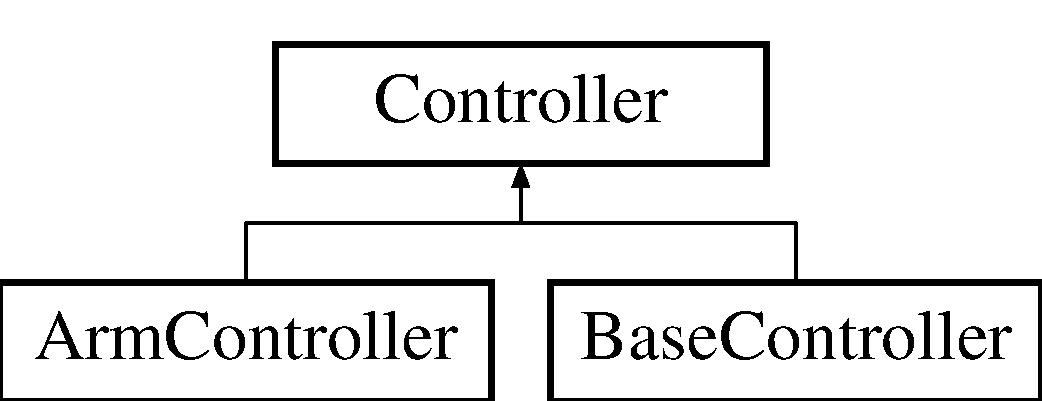
\includegraphics[height=2.000000cm]{classController}
\end{center}
\end{figure}
\subsection*{\-Métodos públicos}
\begin{DoxyCompactItemize}
\item 
\hypertarget{classController_a0a6ee42fa057aa2a57ef63b1303bf869}{{\bfseries \-Controller} (\hyperlink{classdfv_1_1XsensListener}{dfv\-::\-Xsens\-Listener} \&sensors\-\_\-, \hyperlink{classdfv_1_1Youbot}{dfv\-::\-Youbot} \&youbot\-\_\-)}\label{classController_a0a6ee42fa057aa2a57ef63b1303bf869}

\item 
\hypertarget{classController_a4b66f9c3177c6c87d746b71166b0638a}{virtual bool {\bfseries \-On\-Init} ()}\label{classController_a4b66f9c3177c6c87d746b71166b0638a}

\item 
\hypertarget{classController_affb40952c110db0d6660f021fc606d9b}{virtual std\-::vector$<$ float $>$ {\bfseries \-On\-Update} ()}\label{classController_affb40952c110db0d6660f021fc606d9b}

\item 
\hypertarget{classController_a5ce1aa0f511d51de499bad6e8bda1891}{std\-::vector$<$ float $>$ {\bfseries \-Get\-State} () const }\label{classController_a5ce1aa0f511d51de499bad6e8bda1891}

\item 
\hypertarget{classController_a6945e5f9537d48b2ac073a2d530b1ef7}{unsigned int {\bfseries \-Get\-Frame} () const }\label{classController_a6945e5f9537d48b2ac073a2d530b1ef7}

\end{DoxyCompactItemize}
\subsection*{\-Atributos protegidos}
\begin{DoxyCompactItemize}
\item 
\hypertarget{classController_a4d498383044891557b80a6b42583ba74}{std\-::vector$<$ float $>$ {\bfseries state}}\label{classController_a4d498383044891557b80a6b42583ba74}

\item 
\hypertarget{classController_aee31b087593ef8305ff0a53403839282}{unsigned int {\bfseries frame}}\label{classController_aee31b087593ef8305ff0a53403839282}

\item 
\hypertarget{classController_af615f2f2b4bb6c1cadefc6dee7df856e}{\hyperlink{classdfv_1_1XsensListener}{dfv\-::\-Xsens\-Listener} \& {\bfseries sensors}}\label{classController_af615f2f2b4bb6c1cadefc6dee7df856e}

\item 
\hypertarget{classController_a82a5fc973ed64cf343a0945c6b3874ab}{\hyperlink{classdfv_1_1Youbot}{dfv\-::\-Youbot} \& {\bfseries youbot}}\label{classController_a82a5fc973ed64cf343a0945c6b3874ab}

\end{DoxyCompactItemize}


\-La documentación para esta clase fue generada a partir del siguiente fichero\-:\begin{DoxyCompactItemize}
\item 
youbot\-\_\-controller/include/youbot\-\_\-controller/controller.\-h\end{DoxyCompactItemize}

\hypertarget{classxsens_1_1Driver}{\section{\-Referencia de la \-Clase xsens\-:\-:\-Driver}
\label{classxsens_1_1Driver}\index{xsens\-::\-Driver@{xsens\-::\-Driver}}
}
\subsection*{\-Métodos públicos}
\begin{DoxyCompactItemize}
\item 
\hypertarget{classxsens_1_1Driver_a49c7cd43d2a9afe015544bd26c2621e9}{bool {\bfseries \-Initialize} ()}\label{classxsens_1_1Driver_a49c7cd43d2a9afe015544bd26c2621e9}

\item 
\hypertarget{classxsens_1_1Driver_afd72f6bbfcf7941840ad66ede6f7f14d}{void {\bfseries \-Set\-Output\-Mode} (\hyperlink{cmtdef_8h_a85df1cdea0bf11e38292e3cd5d69e747}{\-Cmt\-Output\-Mode} output\-\_\-mode)}\label{classxsens_1_1Driver_afd72f6bbfcf7941840ad66ede6f7f14d}

\item 
\hypertarget{classxsens_1_1Driver_af79d1a877cfb40cb97f385190d8563cf}{\hyperlink{cmtdef_8h_a85df1cdea0bf11e38292e3cd5d69e747}{\-Cmt\-Output\-Mode} {\bfseries \-Get\-Output\-Mode} () const }\label{classxsens_1_1Driver_af79d1a877cfb40cb97f385190d8563cf}

\item 
\hypertarget{classxsens_1_1Driver_aabdab2e0b3c04b383693df5b5478e078}{void {\bfseries \-Set\-Output\-Settings} (\hyperlink{cmtdef_8h_a4125efede0d0948ee49291165a1d089b}{\-Cmt\-Output\-Settings} output\-\_\-settings)}\label{classxsens_1_1Driver_aabdab2e0b3c04b383693df5b5478e078}

\item 
\hypertarget{classxsens_1_1Driver_ab29f3f14aba8d75efea5f189ddb79c55}{\hyperlink{cmtdef_8h_a4125efede0d0948ee49291165a1d089b}{\-Cmt\-Output\-Settings} {\bfseries \-Get\-Output\-Settings} () const }\label{classxsens_1_1Driver_ab29f3f14aba8d75efea5f189ddb79c55}

\item 
\hypertarget{classxsens_1_1Driver_ab61c542896ab795ac8a3397a4b79688b}{void {\bfseries \-Set\-Output\-Mode} (unsigned int index, \hyperlink{cmtdef_8h_a85df1cdea0bf11e38292e3cd5d69e747}{\-Cmt\-Output\-Mode} output\-\_\-mode)}\label{classxsens_1_1Driver_ab61c542896ab795ac8a3397a4b79688b}

\item 
\hypertarget{classxsens_1_1Driver_a8ea8faa3a30cb87f6c879b988c9a4646}{\hyperlink{cmtdef_8h_a85df1cdea0bf11e38292e3cd5d69e747}{\-Cmt\-Output\-Mode} {\bfseries \-Get\-Output\-Mode} (unsigned int index) const }\label{classxsens_1_1Driver_a8ea8faa3a30cb87f6c879b988c9a4646}

\item 
\hypertarget{classxsens_1_1Driver_a6e85c06b86f6a0ff801bc9ab13e13db9}{void {\bfseries \-Set\-Output\-Settings} (unsigned int index, \hyperlink{cmtdef_8h_a4125efede0d0948ee49291165a1d089b}{\-Cmt\-Output\-Settings} output\-\_\-settings)}\label{classxsens_1_1Driver_a6e85c06b86f6a0ff801bc9ab13e13db9}

\item 
\hypertarget{classxsens_1_1Driver_ab20d691280d7136335b14e0b87be7344}{\hyperlink{cmtdef_8h_a4125efede0d0948ee49291165a1d089b}{\-Cmt\-Output\-Settings} {\bfseries \-Get\-Output\-Settings} (unsigned int index) const }\label{classxsens_1_1Driver_ab20d691280d7136335b14e0b87be7344}

\item 
\hypertarget{classxsens_1_1Driver_accc978728d1f66d3c29eb03d7808f00d}{void {\bfseries \-Set\-Alignment\-Matrix} (unsigned int sensor\-\_\-index, \hyperlink{structCmtMatrix}{\-Cmt\-Matrix} alignment\-\_\-matrix)}\label{classxsens_1_1Driver_accc978728d1f66d3c29eb03d7808f00d}

\item 
\hypertarget{classxsens_1_1Driver_a38ce38dd23ff1f24d81ad76df422d2ba}{bool {\bfseries \-Spin\-Once} ()}\label{classxsens_1_1Driver_a38ce38dd23ff1f24d81ad76df422d2ba}

\item 
\hypertarget{classxsens_1_1Driver_ac3d17b16782f4f21a00e81a5cc16b8d0}{bool {\bfseries \-Retrieve\-Data} ()}\label{classxsens_1_1Driver_ac3d17b16782f4f21a00e81a5cc16b8d0}

\item 
\hypertarget{classxsens_1_1Driver_a8e08abdb1ef1c858b0c588631ff3f1e3}{unsigned int {\bfseries \-Get\-Mt\-Count} ()}\label{classxsens_1_1Driver_a8e08abdb1ef1c858b0c588631ff3f1e3}

\item 
\hypertarget{classxsens_1_1Driver_aa41661edec8bdb1f13decdd999f26d1f}{\hyperlink{cmtdef_8h_a85df1cdea0bf11e38292e3cd5d69e747}{\-Cmt\-Output\-Mode} {\bfseries \-Get\-Output\-Mode} ()}\label{classxsens_1_1Driver_aa41661edec8bdb1f13decdd999f26d1f}

\item 
\hypertarget{classxsens_1_1Driver_aa841e918ab6631687c437eaf633362ff}{\hyperlink{cmtdef_8h_a4125efede0d0948ee49291165a1d089b}{\-Cmt\-Output\-Settings} {\bfseries \-Get\-Output\-Settings} ()}\label{classxsens_1_1Driver_aa841e918ab6631687c437eaf633362ff}

\item 
\hypertarget{classxsens_1_1Driver_a4119fe8be2719bb96fd04ece397b6ae5}{\hyperlink{structCmtQuat}{\-Cmt\-Quat} \& {\bfseries \-Get\-Ori\-Quat} (int mt\-\_\-index=0)}\label{classxsens_1_1Driver_a4119fe8be2719bb96fd04ece397b6ae5}

\item 
\hypertarget{classxsens_1_1Driver_a197277222d62faac554adc3e4f69125b}{\hyperlink{structCmtMatrix}{\-Cmt\-Matrix} \& {\bfseries \-Get\-Ori\-Matrix} (int mt\-\_\-index=0)}\label{classxsens_1_1Driver_a197277222d62faac554adc3e4f69125b}

\item 
\hypertarget{classxsens_1_1Driver_a98773334d95ae6372ce3f7ef78ecfaae}{\hyperlink{structCmtEuler}{\-Cmt\-Euler} \& {\bfseries \-Get\-Ori\-Euler} (int mt\-\_\-index=0)}\label{classxsens_1_1Driver_a98773334d95ae6372ce3f7ef78ecfaae}

\item 
\hypertarget{classxsens_1_1Driver_aeb9ce05d9948c871ec6f5d2750ea3996}{\hyperlink{structCmtRawData}{\-Cmt\-Raw\-Data} \& {\bfseries \-Get\-Raw\-Data} (int mt\-\_\-index=0)}\label{classxsens_1_1Driver_aeb9ce05d9948c871ec6f5d2750ea3996}

\item 
\hypertarget{classxsens_1_1Driver_a50ec7c3dc6033a106d334231954ec1f5}{\hyperlink{structCmtCalData}{\-Cmt\-Cal\-Data} \& {\bfseries \-Get\-Cal\-Data} (int mt\-\_\-index=0)}\label{classxsens_1_1Driver_a50ec7c3dc6033a106d334231954ec1f5}

\item 
\hypertarget{classxsens_1_1Driver_aa90dddcdad4e1a4e26e6e552810056d0}{\hyperlink{structCmtVector}{\-Cmt\-Vector} \& {\bfseries \-Get\-Position\-L\-L\-A} (int mt\-\_\-index=0)}\label{classxsens_1_1Driver_aa90dddcdad4e1a4e26e6e552810056d0}

\item 
\hypertarget{classxsens_1_1Driver_a160254b504179be941c05be6660f7410}{\hyperlink{structCmtGpsPvtData}{\-Cmt\-Gps\-Pvt\-Data} \& {\bfseries \-Get\-Gps\-Pvt\-Data} (int mt\-\_\-index=0)}\label{classxsens_1_1Driver_a160254b504179be941c05be6660f7410}

\end{DoxyCompactItemize}
\subsection*{\-Atributos públicos}
\begin{DoxyCompactItemize}
\item 
\hypertarget{classxsens_1_1Driver_a243584c0cd88ba7b4794f0802bbaf884}{std\-::vector$<$ \hyperlink{classxsens_1_1Sensor}{\-Sensor} $>$ {\bfseries v\-\_\-sensors}}\label{classxsens_1_1Driver_a243584c0cd88ba7b4794f0802bbaf884}

\end{DoxyCompactItemize}


\-La documentación para esta clase fue generada a partir del siguiente fichero\-:\begin{DoxyCompactItemize}
\item 
xsens\-\_\-driver/include/xsens\-\_\-driver/xsens\-\_\-driver.\-h\end{DoxyCompactItemize}

\hypertarget{classxsens_1_1Exception}{\section{\-Referencia de la \-Clase xsens\-:\-:\-Exception}
\label{classxsens_1_1Exception}\index{xsens\-::\-Exception@{xsens\-::\-Exception}}
}
\subsection*{\-Métodos públicos}
\begin{DoxyCompactItemize}
\item 
\hypertarget{classxsens_1_1Exception_acd82158b8e4697e3a271555a8ea5049b}{{\bfseries \-Exception} (const std\-::string \&what)}\label{classxsens_1_1Exception_acd82158b8e4697e3a271555a8ea5049b}

\item 
\hypertarget{classxsens_1_1Exception_a64dc5acf4db2b1dc141e771dbb2c9034}{{\bfseries \-Exception} (const \hyperlink{classxsens_1_1Exception}{\-Exception} \&ex)}\label{classxsens_1_1Exception_a64dc5acf4db2b1dc141e771dbb2c9034}

\item 
\hypertarget{classxsens_1_1Exception_ac98e6d523db09bae3eb76999290e58ff}{virtual const char $\ast$ {\bfseries what} () const   throw ()}\label{classxsens_1_1Exception_ac98e6d523db09bae3eb76999290e58ff}

\end{DoxyCompactItemize}


\-La documentación para esta clase fue generada a partir del siguiente fichero\-:\begin{DoxyCompactItemize}
\item 
xsens\-\_\-driver/include/xsens\-\_\-driver/xsens\-\_\-exception.\-h\end{DoxyCompactItemize}

\hypertarget{classxsens_1_1FifoQueue}{\section{\-Referencia de la plantilla de la \-Clase xsens\-:\-:\-Fifo\-Queue$<$ \-T, \-E $>$}
\label{classxsens_1_1FifoQueue}\index{xsens\-::\-Fifo\-Queue$<$ T, E $>$@{xsens\-::\-Fifo\-Queue$<$ T, E $>$}}
}


\-A \-F\-I\-F\-O queue with limited length (cyclic).  




{\ttfamily \#include $<$xsens\-\_\-fifoqueue.\-h$>$}

\subsection*{\-Tipos públicos}
\begin{DoxyCompactItemize}
\item 
\hypertarget{classxsens_1_1FifoQueue_a61949842c92df50f702496096b9d5069}{typedef \-T \hyperlink{classxsens_1_1FifoQueue_a61949842c92df50f702496096b9d5069}{value\-\_\-type}}\label{classxsens_1_1FifoQueue_a61949842c92df50f702496096b9d5069}

\begin{DoxyCompactList}\small\item\em \-The type of the value stored in this queue. \end{DoxyCompactList}\item 
\hypertarget{classxsens_1_1FifoQueue_a6a595ab989816ba96cf0cbfa4d39b0b1}{typedef size\-\_\-t \hyperlink{classxsens_1_1FifoQueue_a6a595ab989816ba96cf0cbfa4d39b0b1}{size\-\_\-type}}\label{classxsens_1_1FifoQueue_a6a595ab989816ba96cf0cbfa4d39b0b1}

\begin{DoxyCompactList}\small\item\em \-The type of a 'size' value. \end{DoxyCompactList}\end{DoxyCompactItemize}
\subsection*{\-Métodos públicos}
\begin{DoxyCompactItemize}
\item 
\hypertarget{classxsens_1_1FifoQueue_aba62295440c162d8d5cbab74bf09e53e}{\hyperlink{classxsens_1_1FifoQueue_aba62295440c162d8d5cbab74bf09e53e}{\-Fifo\-Queue} (\hyperlink{classxsens_1_1FifoQueue_a6a595ab989816ba96cf0cbfa4d39b0b1}{size\-\_\-type} \hyperlink{classxsens_1_1FifoQueue_abdc9950e2a5833b2520b83bc1daee995}{size}=16, bool del\-On\-Overwrite=true)}\label{classxsens_1_1FifoQueue_aba62295440c162d8d5cbab74bf09e53e}

\begin{DoxyCompactList}\small\item\em \-Create an empty queue with capacity size. \end{DoxyCompactList}\item 
\hypertarget{classxsens_1_1FifoQueue_a848cf288889b759f331cd35532f95832}{{\footnotesize template$<$bool \-E2$>$ }\\\hyperlink{classxsens_1_1FifoQueue_a848cf288889b759f331cd35532f95832}{\-Fifo\-Queue} (const \hyperlink{classxsens_1_1FifoQueue}{\-Fifo\-Queue}$<$ \-T, \-E2 $>$ \&q)}\label{classxsens_1_1FifoQueue_a848cf288889b759f331cd35532f95832}

\begin{DoxyCompactList}\small\item\em \-The copy constructor. \end{DoxyCompactList}\item 
\hypertarget{classxsens_1_1FifoQueue_a7127b28f9107af06ae9590a95ad1c89f}{void {\bfseries erase\-And\-Clear} (void)}\label{classxsens_1_1FifoQueue_a7127b28f9107af06ae9590a95ad1c89f}

\item 
\hypertarget{classxsens_1_1FifoQueue_a9bc44c0ea07343fb6b2f594208174a32}{\hyperlink{classxsens_1_1FifoQueue_a9bc44c0ea07343fb6b2f594208174a32}{$\sim$\-Fifo\-Queue} ()}\label{classxsens_1_1FifoQueue_a9bc44c0ea07343fb6b2f594208174a32}

\begin{DoxyCompactList}\small\item\em \-The destructor. \end{DoxyCompactList}\item 
\hypertarget{classxsens_1_1FifoQueue_a602b54c4b491ec24fe3bc59a5d9ec69a}{{\footnotesize template$<$bool \-E2$>$ }\\\hyperlink{classxsens_1_1FifoQueue}{\-Fifo\-Queue}$<$ \-T, \-E $>$ \& \hyperlink{classxsens_1_1FifoQueue_a602b54c4b491ec24fe3bc59a5d9ec69a}{operator=} (const \hyperlink{classxsens_1_1FifoQueue}{\-Fifo\-Queue}$<$ \-T, \-E2 $>$ \&q)}\label{classxsens_1_1FifoQueue_a602b54c4b491ec24fe3bc59a5d9ec69a}

\begin{DoxyCompactList}\small\item\em \-The assignment operator. \end{DoxyCompactList}\item 
\hypertarget{classxsens_1_1FifoQueue_a2c02ee912d71b2a476e2513824dee88a}{void \hyperlink{classxsens_1_1FifoQueue_a2c02ee912d71b2a476e2513824dee88a}{resize} (const size\-\_\-t \hyperlink{classxsens_1_1FifoQueue_abdc9950e2a5833b2520b83bc1daee995}{size})}\label{classxsens_1_1FifoQueue_a2c02ee912d71b2a476e2513824dee88a}

\begin{DoxyCompactList}\small\item\em \-Resize the queue, note that this function clears the queue. \end{DoxyCompactList}\item 
\hypertarget{classxsens_1_1FifoQueue_af133de61bb276774138f1aab187b2918}{bool \hyperlink{classxsens_1_1FifoQueue_af133de61bb276774138f1aab187b2918}{empty} () const }\label{classxsens_1_1FifoQueue_af133de61bb276774138f1aab187b2918}

\begin{DoxyCompactList}\small\item\em \-Return true if the queue is empty. \end{DoxyCompactList}\item 
\hypertarget{classxsens_1_1FifoQueue_abdc9950e2a5833b2520b83bc1daee995}{\hyperlink{classxsens_1_1FifoQueue_a6a595ab989816ba96cf0cbfa4d39b0b1}{size\-\_\-type} \hyperlink{classxsens_1_1FifoQueue_abdc9950e2a5833b2520b83bc1daee995}{size} () const }\label{classxsens_1_1FifoQueue_abdc9950e2a5833b2520b83bc1daee995}

\begin{DoxyCompactList}\small\item\em \-Return the maximum number of elements in the queue. \end{DoxyCompactList}\item 
\hypertarget{classxsens_1_1FifoQueue_adade9fdae6da5cb6c3186f9fa15fd118}{\hyperlink{classxsens_1_1FifoQueue_a6a595ab989816ba96cf0cbfa4d39b0b1}{size\-\_\-type} \hyperlink{classxsens_1_1FifoQueue_adade9fdae6da5cb6c3186f9fa15fd118}{length} () const }\label{classxsens_1_1FifoQueue_adade9fdae6da5cb6c3186f9fa15fd118}

\begin{DoxyCompactList}\small\item\em \-Return the number of elements currnetly in the queue. \end{DoxyCompactList}\item 
\hypertarget{classxsens_1_1FifoQueue_a41ec39c634b1b6c9fdb195b0e0bf9b6f}{\hyperlink{classxsens_1_1FifoQueue_a61949842c92df50f702496096b9d5069}{value\-\_\-type} \& \hyperlink{classxsens_1_1FifoQueue_a41ec39c634b1b6c9fdb195b0e0bf9b6f}{front} ()}\label{classxsens_1_1FifoQueue_a41ec39c634b1b6c9fdb195b0e0bf9b6f}

\begin{DoxyCompactList}\small\item\em \-Return the oldest element in the queue. \end{DoxyCompactList}\item 
\hypertarget{classxsens_1_1FifoQueue_a50ca25fc36e08035375844ecdda577b4}{const \hyperlink{classxsens_1_1FifoQueue_a61949842c92df50f702496096b9d5069}{value\-\_\-type} \& \hyperlink{classxsens_1_1FifoQueue_a50ca25fc36e08035375844ecdda577b4}{front} () const }\label{classxsens_1_1FifoQueue_a50ca25fc36e08035375844ecdda577b4}

\begin{DoxyCompactList}\small\item\em \-Return the oldest element in the queue. \end{DoxyCompactList}\item 
\hypertarget{classxsens_1_1FifoQueue_a7954676d04eae451a35fae55e8e5c6e9}{\hyperlink{classxsens_1_1FifoQueue_a61949842c92df50f702496096b9d5069}{value\-\_\-type} \& \hyperlink{classxsens_1_1FifoQueue_a7954676d04eae451a35fae55e8e5c6e9}{back} ()}\label{classxsens_1_1FifoQueue_a7954676d04eae451a35fae55e8e5c6e9}

\begin{DoxyCompactList}\small\item\em \-Return the newest element in the queue. \end{DoxyCompactList}\item 
\hypertarget{classxsens_1_1FifoQueue_a1734249c16d89e99161b515f6517400b}{const \hyperlink{classxsens_1_1FifoQueue_a61949842c92df50f702496096b9d5069}{value\-\_\-type} \& \hyperlink{classxsens_1_1FifoQueue_a1734249c16d89e99161b515f6517400b}{back} () const }\label{classxsens_1_1FifoQueue_a1734249c16d89e99161b515f6517400b}

\begin{DoxyCompactList}\small\item\em \-Return the newest element in the queue. \end{DoxyCompactList}\item 
\hypertarget{classxsens_1_1FifoQueue_a15f1c61dae6d5811de3eeddca1a392b0}{void \hyperlink{classxsens_1_1FifoQueue_a15f1c61dae6d5811de3eeddca1a392b0}{push} (const \hyperlink{classxsens_1_1FifoQueue_a61949842c92df50f702496096b9d5069}{value\-\_\-type} \&x)}\label{classxsens_1_1FifoQueue_a15f1c61dae6d5811de3eeddca1a392b0}

\begin{DoxyCompactList}\small\item\em \-Insert x at the back of the queue. \end{DoxyCompactList}\item 
\hypertarget{classxsens_1_1FifoQueue_a88e76121245a40be2bcf971bb94860f3}{void \hyperlink{classxsens_1_1FifoQueue_a88e76121245a40be2bcf971bb94860f3}{pop} (void)}\label{classxsens_1_1FifoQueue_a88e76121245a40be2bcf971bb94860f3}

\begin{DoxyCompactList}\small\item\em \-Remove the element at the front of the queue. \end{DoxyCompactList}\item 
\hypertarget{classxsens_1_1FifoQueue_adee7b4f0f0c30d8b29360755b4ef1e62}{void \hyperlink{classxsens_1_1FifoQueue_adee7b4f0f0c30d8b29360755b4ef1e62}{pop\-Back} (void)}\label{classxsens_1_1FifoQueue_adee7b4f0f0c30d8b29360755b4ef1e62}

\begin{DoxyCompactList}\small\item\em \-Remove the element at the back of the queue. \end{DoxyCompactList}\item 
\hypertarget{classxsens_1_1FifoQueue_ac08368440cbb0080eb970878bcc85eaa}{const \hyperlink{classxsens_1_1FifoQueue_a61949842c92df50f702496096b9d5069}{value\-\_\-type} \& \hyperlink{classxsens_1_1FifoQueue_ac08368440cbb0080eb970878bcc85eaa}{operator\mbox{[}$\,$\mbox{]}} (size\-\_\-t index) const }\label{classxsens_1_1FifoQueue_ac08368440cbb0080eb970878bcc85eaa}

\begin{DoxyCompactList}\small\item\em \-Return the index'th oldest item from the queue. \end{DoxyCompactList}\item 
\hypertarget{classxsens_1_1FifoQueue_a18a1acd59d9f6e0b7b52915134e4f3d3}{\hyperlink{classxsens_1_1FifoQueue_a61949842c92df50f702496096b9d5069}{value\-\_\-type} \& \hyperlink{classxsens_1_1FifoQueue_a18a1acd59d9f6e0b7b52915134e4f3d3}{operator\mbox{[}$\,$\mbox{]}} (size\-\_\-t index)}\label{classxsens_1_1FifoQueue_a18a1acd59d9f6e0b7b52915134e4f3d3}

\begin{DoxyCompactList}\small\item\em \-Return the index'th oldest item from the queue. \end{DoxyCompactList}\item 
\hypertarget{classxsens_1_1FifoQueue_a4ca3418799bc8e72e96dae1ede9b08ef}{void {\bfseries clear} (void)}\label{classxsens_1_1FifoQueue_a4ca3418799bc8e72e96dae1ede9b08ef}

\item 
\hypertarget{classxsens_1_1FifoQueue_af97f5a1f8232edf50b1d37b365ddb49a}{void {\bfseries remove} (size\-\_\-t index)}\label{classxsens_1_1FifoQueue_af97f5a1f8232edf50b1d37b365ddb49a}

\end{DoxyCompactItemize}
\subsection*{\-Atributos protegidos}
\begin{DoxyCompactItemize}
\item 
\hypertarget{classxsens_1_1FifoQueue_a92c68d73af943dca929c9dbabe90042c}{size\-\_\-t {\bfseries m\-\_\-max\-Count}}\label{classxsens_1_1FifoQueue_a92c68d73af943dca929c9dbabe90042c}

\item 
\hypertarget{classxsens_1_1FifoQueue_ae333afd4993d7558116d3fcb42ed1143}{size\-\_\-t {\bfseries m\-\_\-current\-Count}}\label{classxsens_1_1FifoQueue_ae333afd4993d7558116d3fcb42ed1143}

\item 
\hypertarget{classxsens_1_1FifoQueue_ab28ce4c8eac78b214daf6ddb5d722af8}{size\-\_\-t {\bfseries m\-\_\-first}}\label{classxsens_1_1FifoQueue_ab28ce4c8eac78b214daf6ddb5d722af8}

\item 
\hypertarget{classxsens_1_1FifoQueue_a669d5fc4b869368e6de3452cccc7a422}{bool {\bfseries m\-\_\-delete\-On\-Overwrite}}\label{classxsens_1_1FifoQueue_a669d5fc4b869368e6de3452cccc7a422}

\item 
\hypertarget{classxsens_1_1FifoQueue_a254fc271e83f10761f8c219fd96b35f8}{\-T $\ast$ {\bfseries m\-\_\-list}}\label{classxsens_1_1FifoQueue_a254fc271e83f10761f8c219fd96b35f8}

\end{DoxyCompactItemize}


\subsection{\-Descripción detallada}
\subsubsection*{template$<$class \-T, bool \-E = true$>$class xsens\-::\-Fifo\-Queue$<$ T, E $>$}

\-A \-F\-I\-F\-O queue with limited length (cyclic). 

\-The class is based on the \-S\-T\-L queue class, but has a limited size. \-If more items are inserted than would fit, the oldest item is overwritten. \-The class can only handle pointer types. 

\-La documentación para esta clase fue generada a partir del siguiente fichero\-:\begin{DoxyCompactItemize}
\item 
xsens\-\_\-driver/include/xsens\-\_\-driver/\hyperlink{xsens__fifoqueue_8h}{xsens\-\_\-fifoqueue.\-h}\end{DoxyCompactItemize}

\hypertarget{classxsens_1_1FifoQueueBasic}{\section{\-Referencia de la plantilla de la \-Clase xsens\-:\-:\-Fifo\-Queue\-Basic$<$ \-T $>$}
\label{classxsens_1_1FifoQueueBasic}\index{xsens\-::\-Fifo\-Queue\-Basic$<$ T $>$@{xsens\-::\-Fifo\-Queue\-Basic$<$ T $>$}}
}


\-A \-F\-I\-F\-O queue with limited length (cyclic).  




{\ttfamily \#include $<$xsens\-\_\-fifoqueue.\-h$>$}

\subsection*{\-Tipos públicos}
\begin{DoxyCompactItemize}
\item 
\hypertarget{classxsens_1_1FifoQueueBasic_a4952f1bac21ff075e2b7667cbca0cd0e}{typedef \-T \hyperlink{classxsens_1_1FifoQueueBasic_a4952f1bac21ff075e2b7667cbca0cd0e}{value\-\_\-type}}\label{classxsens_1_1FifoQueueBasic_a4952f1bac21ff075e2b7667cbca0cd0e}

\begin{DoxyCompactList}\small\item\em \-The type of the value stored in this queue. \end{DoxyCompactList}\item 
\hypertarget{classxsens_1_1FifoQueueBasic_abef5a7d633ee8b57a33360bf3b3efdef}{typedef size\-\_\-t \hyperlink{classxsens_1_1FifoQueueBasic_abef5a7d633ee8b57a33360bf3b3efdef}{size\-\_\-type}}\label{classxsens_1_1FifoQueueBasic_abef5a7d633ee8b57a33360bf3b3efdef}

\begin{DoxyCompactList}\small\item\em \-The type of a 'size' value. \end{DoxyCompactList}\end{DoxyCompactItemize}
\subsection*{\-Métodos públicos}
\begin{DoxyCompactItemize}
\item 
\hypertarget{classxsens_1_1FifoQueueBasic_a4943e456da5439290e6e2e705dc350db}{\hyperlink{classxsens_1_1FifoQueueBasic_a4943e456da5439290e6e2e705dc350db}{\-Fifo\-Queue\-Basic} (\hyperlink{classxsens_1_1FifoQueueBasic_abef5a7d633ee8b57a33360bf3b3efdef}{size\-\_\-type} \hyperlink{classxsens_1_1FifoQueueBasic_a918b730b9085edd926404337d588d002}{size}=16)}\label{classxsens_1_1FifoQueueBasic_a4943e456da5439290e6e2e705dc350db}

\begin{DoxyCompactList}\small\item\em \-Create an empty queue with capacity 'size'. \end{DoxyCompactList}\item 
\hypertarget{classxsens_1_1FifoQueueBasic_a9f922ea1e1773b296304deabf6e2bde3}{\hyperlink{classxsens_1_1FifoQueueBasic_a9f922ea1e1773b296304deabf6e2bde3}{\-Fifo\-Queue\-Basic} (const \hyperlink{classxsens_1_1FifoQueueBasic}{\-Fifo\-Queue\-Basic}$<$ \-T $>$ \&q)}\label{classxsens_1_1FifoQueueBasic_a9f922ea1e1773b296304deabf6e2bde3}

\begin{DoxyCompactList}\small\item\em \-The copy constructor. \end{DoxyCompactList}\item 
\hypertarget{classxsens_1_1FifoQueueBasic_a26b594e18f5b4f0a3a21eb0c82928590}{void {\bfseries erase\-And\-Clear} (void)}\label{classxsens_1_1FifoQueueBasic_a26b594e18f5b4f0a3a21eb0c82928590}

\item 
\hypertarget{classxsens_1_1FifoQueueBasic_a0e9808c170b05a5616c193525d1b324c}{\hyperlink{classxsens_1_1FifoQueueBasic_a0e9808c170b05a5616c193525d1b324c}{$\sim$\-Fifo\-Queue\-Basic} ()}\label{classxsens_1_1FifoQueueBasic_a0e9808c170b05a5616c193525d1b324c}

\begin{DoxyCompactList}\small\item\em \-The destructor. \end{DoxyCompactList}\item 
\hypertarget{classxsens_1_1FifoQueueBasic_aa53f27abd204394954d2a15b03eeb025}{\hyperlink{classxsens_1_1FifoQueueBasic}{\-Fifo\-Queue\-Basic}$<$ \-T $>$ \& \hyperlink{classxsens_1_1FifoQueueBasic_aa53f27abd204394954d2a15b03eeb025}{operator=} (const \hyperlink{classxsens_1_1FifoQueueBasic}{\-Fifo\-Queue\-Basic}$<$ \-T $>$ \&q)}\label{classxsens_1_1FifoQueueBasic_aa53f27abd204394954d2a15b03eeb025}

\begin{DoxyCompactList}\small\item\em \-The assignment operator. \end{DoxyCompactList}\item 
\hypertarget{classxsens_1_1FifoQueueBasic_a65b60d55a8f43de327a8e74d89a3ab36}{void \hyperlink{classxsens_1_1FifoQueueBasic_a65b60d55a8f43de327a8e74d89a3ab36}{resize} (const size\-\_\-t \hyperlink{classxsens_1_1FifoQueueBasic_a918b730b9085edd926404337d588d002}{size})}\label{classxsens_1_1FifoQueueBasic_a65b60d55a8f43de327a8e74d89a3ab36}

\begin{DoxyCompactList}\small\item\em \-Resize the queue, note that this function clears the queue. \end{DoxyCompactList}\item 
\hypertarget{classxsens_1_1FifoQueueBasic_aefc810309cd8e547fe6518d09d3ba825}{bool \hyperlink{classxsens_1_1FifoQueueBasic_aefc810309cd8e547fe6518d09d3ba825}{empty} () const }\label{classxsens_1_1FifoQueueBasic_aefc810309cd8e547fe6518d09d3ba825}

\begin{DoxyCompactList}\small\item\em \-Return true if the queue is empty. \end{DoxyCompactList}\item 
\hypertarget{classxsens_1_1FifoQueueBasic_a918b730b9085edd926404337d588d002}{\hyperlink{classxsens_1_1FifoQueueBasic_abef5a7d633ee8b57a33360bf3b3efdef}{size\-\_\-type} \hyperlink{classxsens_1_1FifoQueueBasic_a918b730b9085edd926404337d588d002}{size} () const }\label{classxsens_1_1FifoQueueBasic_a918b730b9085edd926404337d588d002}

\begin{DoxyCompactList}\small\item\em \-Return the maximum number of elements in the queue. \end{DoxyCompactList}\item 
\hypertarget{classxsens_1_1FifoQueueBasic_a3436798e8adf684fc62dce29feb6ade7}{\hyperlink{classxsens_1_1FifoQueueBasic_abef5a7d633ee8b57a33360bf3b3efdef}{size\-\_\-type} \hyperlink{classxsens_1_1FifoQueueBasic_a3436798e8adf684fc62dce29feb6ade7}{length} () const }\label{classxsens_1_1FifoQueueBasic_a3436798e8adf684fc62dce29feb6ade7}

\begin{DoxyCompactList}\small\item\em \-Return the number of elements currently in the queue. \end{DoxyCompactList}\item 
\hypertarget{classxsens_1_1FifoQueueBasic_a723b25ff30a6da3aec91766a06abd229}{\hyperlink{classxsens_1_1FifoQueueBasic_a4952f1bac21ff075e2b7667cbca0cd0e}{value\-\_\-type} \& \hyperlink{classxsens_1_1FifoQueueBasic_a723b25ff30a6da3aec91766a06abd229}{front} ()}\label{classxsens_1_1FifoQueueBasic_a723b25ff30a6da3aec91766a06abd229}

\begin{DoxyCompactList}\small\item\em \-Return the oldest element in the queue. \end{DoxyCompactList}\item 
\hypertarget{classxsens_1_1FifoQueueBasic_ad8a5f0ae3e4062627e91fc6b053e645d}{const \hyperlink{classxsens_1_1FifoQueueBasic_a4952f1bac21ff075e2b7667cbca0cd0e}{value\-\_\-type} \& \hyperlink{classxsens_1_1FifoQueueBasic_ad8a5f0ae3e4062627e91fc6b053e645d}{front} () const }\label{classxsens_1_1FifoQueueBasic_ad8a5f0ae3e4062627e91fc6b053e645d}

\begin{DoxyCompactList}\small\item\em \-Return the oldest element in the queue. \end{DoxyCompactList}\item 
\hypertarget{classxsens_1_1FifoQueueBasic_a33639a8731cc2590153dd95492459ea0}{\hyperlink{classxsens_1_1FifoQueueBasic_a4952f1bac21ff075e2b7667cbca0cd0e}{value\-\_\-type} \& \hyperlink{classxsens_1_1FifoQueueBasic_a33639a8731cc2590153dd95492459ea0}{back} ()}\label{classxsens_1_1FifoQueueBasic_a33639a8731cc2590153dd95492459ea0}

\begin{DoxyCompactList}\small\item\em \-Return the newest element in the queue. \end{DoxyCompactList}\item 
\hypertarget{classxsens_1_1FifoQueueBasic_a1f5bb07419fca39aac16c801a93556b7}{const \hyperlink{classxsens_1_1FifoQueueBasic_a4952f1bac21ff075e2b7667cbca0cd0e}{value\-\_\-type} \& \hyperlink{classxsens_1_1FifoQueueBasic_a1f5bb07419fca39aac16c801a93556b7}{back} () const }\label{classxsens_1_1FifoQueueBasic_a1f5bb07419fca39aac16c801a93556b7}

\begin{DoxyCompactList}\small\item\em \-Return the newest element in the queue. \end{DoxyCompactList}\item 
\hypertarget{classxsens_1_1FifoQueueBasic_a75820c39f6f0eb6fa5c5598b6031e7e4}{void \hyperlink{classxsens_1_1FifoQueueBasic_a75820c39f6f0eb6fa5c5598b6031e7e4}{push} (const \hyperlink{classxsens_1_1FifoQueueBasic_a4952f1bac21ff075e2b7667cbca0cd0e}{value\-\_\-type} \&x)}\label{classxsens_1_1FifoQueueBasic_a75820c39f6f0eb6fa5c5598b6031e7e4}

\begin{DoxyCompactList}\small\item\em \-Insert x at the back of the queue. \end{DoxyCompactList}\item 
\hypertarget{classxsens_1_1FifoQueueBasic_abf8e8b07e6d5a385910392f73f562e52}{void \hyperlink{classxsens_1_1FifoQueueBasic_abf8e8b07e6d5a385910392f73f562e52}{push\-\_\-front} (const \hyperlink{classxsens_1_1FifoQueueBasic_a4952f1bac21ff075e2b7667cbca0cd0e}{value\-\_\-type} \&x)}\label{classxsens_1_1FifoQueueBasic_abf8e8b07e6d5a385910392f73f562e52}

\begin{DoxyCompactList}\small\item\em \-Insert x at the front of the queue (\-L\-I\-F\-O operation). \end{DoxyCompactList}\item 
\hypertarget{classxsens_1_1FifoQueueBasic_aa28bb1cebe3f0e01ff1ec5847697dd70}{void \hyperlink{classxsens_1_1FifoQueueBasic_aa28bb1cebe3f0e01ff1ec5847697dd70}{pop} (void)}\label{classxsens_1_1FifoQueueBasic_aa28bb1cebe3f0e01ff1ec5847697dd70}

\begin{DoxyCompactList}\small\item\em \-Remove the element at the front of the queue. \end{DoxyCompactList}\item 
\hypertarget{classxsens_1_1FifoQueueBasic_a3d9e2c4708d577757281e2bdbaec075e}{void \hyperlink{classxsens_1_1FifoQueueBasic_a3d9e2c4708d577757281e2bdbaec075e}{pop\-Back} (void)}\label{classxsens_1_1FifoQueueBasic_a3d9e2c4708d577757281e2bdbaec075e}

\begin{DoxyCompactList}\small\item\em \-Remove the element at the back of the queue. \end{DoxyCompactList}\item 
\hypertarget{classxsens_1_1FifoQueueBasic_a2173da95e88dcbfddf2638052c9dcc44}{const \hyperlink{classxsens_1_1FifoQueueBasic_a4952f1bac21ff075e2b7667cbca0cd0e}{value\-\_\-type} \& \hyperlink{classxsens_1_1FifoQueueBasic_a2173da95e88dcbfddf2638052c9dcc44}{operator\mbox{[}$\,$\mbox{]}} (size\-\_\-t index) const }\label{classxsens_1_1FifoQueueBasic_a2173da95e88dcbfddf2638052c9dcc44}

\begin{DoxyCompactList}\small\item\em \-Return the index'th oldest item from the queue. \end{DoxyCompactList}\item 
\hypertarget{classxsens_1_1FifoQueueBasic_ac0d554117a06054965a173a3c949f895}{\hyperlink{classxsens_1_1FifoQueueBasic_a4952f1bac21ff075e2b7667cbca0cd0e}{value\-\_\-type} \& \hyperlink{classxsens_1_1FifoQueueBasic_ac0d554117a06054965a173a3c949f895}{operator\mbox{[}$\,$\mbox{]}} (size\-\_\-t index)}\label{classxsens_1_1FifoQueueBasic_ac0d554117a06054965a173a3c949f895}

\begin{DoxyCompactList}\small\item\em \-Return the index'th oldest item from the queue. \end{DoxyCompactList}\item 
\hypertarget{classxsens_1_1FifoQueueBasic_a6e9b68332f69675ea4c06c91898b725c}{void {\bfseries clear} (void)}\label{classxsens_1_1FifoQueueBasic_a6e9b68332f69675ea4c06c91898b725c}

\item 
\hypertarget{classxsens_1_1FifoQueueBasic_ab6ad03db2612b04aa7a79a7573516ea2}{void {\bfseries remove} (size\-\_\-t index)}\label{classxsens_1_1FifoQueueBasic_ab6ad03db2612b04aa7a79a7573516ea2}

\end{DoxyCompactItemize}
\subsection*{\-Atributos protegidos}
\begin{DoxyCompactItemize}
\item 
\hypertarget{classxsens_1_1FifoQueueBasic_a4f40352af305fcc00d029e8e732bed68}{size\-\_\-t {\bfseries m\-\_\-max\-Count}}\label{classxsens_1_1FifoQueueBasic_a4f40352af305fcc00d029e8e732bed68}

\item 
\hypertarget{classxsens_1_1FifoQueueBasic_acdc35d9bf7cd4616ac6f6d12be44c9f5}{size\-\_\-t {\bfseries m\-\_\-current\-Count}}\label{classxsens_1_1FifoQueueBasic_acdc35d9bf7cd4616ac6f6d12be44c9f5}

\item 
\hypertarget{classxsens_1_1FifoQueueBasic_a85c7677c78c9f0e7e2b45a9db3181cae}{size\-\_\-t {\bfseries m\-\_\-first}}\label{classxsens_1_1FifoQueueBasic_a85c7677c78c9f0e7e2b45a9db3181cae}

\item 
\hypertarget{classxsens_1_1FifoQueueBasic_a040a46f15f35e7712bacc1a6a92b3e9a}{\-T $\ast$ {\bfseries m\-\_\-list}}\label{classxsens_1_1FifoQueueBasic_a040a46f15f35e7712bacc1a6a92b3e9a}

\end{DoxyCompactItemize}


\subsection{\-Descripción detallada}
\subsubsection*{template$<$class \-T$>$class xsens\-::\-Fifo\-Queue\-Basic$<$ T $>$}

\-A \-F\-I\-F\-O queue with limited length (cyclic). 

\-The class is based on the \-S\-T\-L queue class, but has a limited size. \-If more items are inserted than would fit, the oldest item is overwritten. \-The class can only handle non-\/pointer types. 

\-La documentación para esta clase fue generada a partir del siguiente fichero\-:\begin{DoxyCompactItemize}
\item 
xsens\-\_\-driver/include/xsens\-\_\-driver/\hyperlink{xsens__fifoqueue_8h}{xsens\-\_\-fifoqueue.\-h}\end{DoxyCompactItemize}

\hypertarget{classdfv_1_1Gripper}{\section{\-Referencia de la \-Clase dfv\-:\-:\-Gripper}
\label{classdfv_1_1Gripper}\index{dfv\-::\-Gripper@{dfv\-::\-Gripper}}
}
\subsection*{\-Tipos públicos}
\begin{DoxyCompactItemize}
\item 
enum {\bfseries \-State} \{ {\bfseries open} =  0, 
{\bfseries closed}
 \}
\end{DoxyCompactItemize}
\subsection*{\-Métodos públicos}
\begin{DoxyCompactItemize}
\item 
\hypertarget{classdfv_1_1Gripper_a332cae0d0403c28abbc6ebbbe23d9c09}{{\bfseries \-Gripper} (ros\-::\-Node\-Handle \&\-\_\-node\-\_\-handle)}\label{classdfv_1_1Gripper_a332cae0d0403c28abbc6ebbbe23d9c09}

\item 
\hypertarget{classdfv_1_1Gripper_a113420d6e814f142851ba071b70c067d}{void {\bfseries \-Open} ()}\label{classdfv_1_1Gripper_a113420d6e814f142851ba071b70c067d}

\item 
\hypertarget{classdfv_1_1Gripper_a0c552cd2c919e72997aa559ccc511242}{void {\bfseries \-Close} ()}\label{classdfv_1_1Gripper_a0c552cd2c919e72997aa559ccc511242}

\end{DoxyCompactItemize}


\-La documentación para esta clase fue generada a partir del siguiente fichero\-:\begin{DoxyCompactItemize}
\item 
dfv/include/dfv/youbot.\-h\end{DoxyCompactItemize}

\hypertarget{classxsens_1_1JanitorClassFunc}{\section{\-Referencia de la plantilla de la \-Clase xsens\-:\-:\-Janitor\-Class\-Func$<$ \-T, \-R $>$}
\label{classxsens_1_1JanitorClassFunc}\index{xsens\-::\-Janitor\-Class\-Func$<$ T, R $>$@{xsens\-::\-Janitor\-Class\-Func$<$ T, R $>$}}
}


\-Class function calling janitor class.  




{\ttfamily \#include $<$xsens\-\_\-janitors.\-h$>$}

\subsection*{\-Tipos públicos}
\begin{DoxyCompactItemize}
\item 
\hypertarget{classxsens_1_1JanitorClassFunc_a30ea6469d27a1ddb625731411dcf4a50}{typedef \-R(\-T\-::$\ast$ {\bfseries t\-\_\-func\-\_\-\-Janitor\-Class\-Func} )(void)}\label{classxsens_1_1JanitorClassFunc_a30ea6469d27a1ddb625731411dcf4a50}

\end{DoxyCompactItemize}
\subsection*{\-Métodos públicos}
\begin{DoxyCompactItemize}
\item 
\hypertarget{classxsens_1_1JanitorClassFunc_a74fa44d8acaa46c40cb5199018e535b6}{{\bfseries \-Janitor\-Class\-Func} (\-T \&control, t\-\_\-func\-\_\-\-Janitor\-Class\-Func func, bool enabl=true)}\label{classxsens_1_1JanitorClassFunc_a74fa44d8acaa46c40cb5199018e535b6}

\item 
\hypertarget{classxsens_1_1JanitorClassFunc_afd298897c201b68ee16fb2e0c36e18fd}{void {\bfseries disable} (void)}\label{classxsens_1_1JanitorClassFunc_afd298897c201b68ee16fb2e0c36e18fd}

\item 
\hypertarget{classxsens_1_1JanitorClassFunc_a1c815a44b79ade44d47bf96325eb4203}{void {\bfseries enable} (void)}\label{classxsens_1_1JanitorClassFunc_a1c815a44b79ade44d47bf96325eb4203}

\end{DoxyCompactItemize}


\subsection{\-Descripción detallada}
\subsubsection*{template$<$class \-T, typename \-R = void$>$class xsens\-::\-Janitor\-Class\-Func$<$ T, R $>$}

\-Class function calling janitor class. 

\-This class can be used to make sure that the given class function is called when the janitor leaves scope. 

\-La documentación para esta clase fue generada a partir del siguiente fichero\-:\begin{DoxyCompactItemize}
\item 
xsens\-\_\-driver/include/xsens\-\_\-driver/\hyperlink{xsens__janitors_8h}{xsens\-\_\-janitors.\-h}\end{DoxyCompactItemize}

\hypertarget{classxsens_1_1JanitorClassFuncP1}{\section{\-Referencia de la plantilla de la \-Clase xsens\-:\-:\-Janitor\-Class\-Func\-P1$<$ \-T, \-P1, \-R $>$}
\label{classxsens_1_1JanitorClassFuncP1}\index{xsens\-::\-Janitor\-Class\-Func\-P1$<$ T, P1, R $>$@{xsens\-::\-Janitor\-Class\-Func\-P1$<$ T, P1, R $>$}}
}


\-Class function calling janitor class with a parameter.  




{\ttfamily \#include $<$xsens\-\_\-janitors.\-h$>$}

\subsection*{\-Tipos públicos}
\begin{DoxyCompactItemize}
\item 
\hypertarget{classxsens_1_1JanitorClassFuncP1_ae1c1b91aa5d0847609c8c566c7786921}{typedef \-R(\-T\-::$\ast$ {\bfseries t\-\_\-func\-\_\-\-Janitor\-Class\-Func} )(\-P1)}\label{classxsens_1_1JanitorClassFuncP1_ae1c1b91aa5d0847609c8c566c7786921}

\end{DoxyCompactItemize}
\subsection*{\-Métodos públicos}
\begin{DoxyCompactItemize}
\item 
\hypertarget{classxsens_1_1JanitorClassFuncP1_aa71ab8a6de75ad75e45cc87a22b4a8de}{{\bfseries \-Janitor\-Class\-Func\-P1} (\-T \&control, \-P1 p1, t\-\_\-func\-\_\-\-Janitor\-Class\-Func func, bool enabl=true)}\label{classxsens_1_1JanitorClassFuncP1_aa71ab8a6de75ad75e45cc87a22b4a8de}

\item 
\hypertarget{classxsens_1_1JanitorClassFuncP1_a4dbcc615b9961b5f0bb6684a7de5aacc}{void {\bfseries disable} (void)}\label{classxsens_1_1JanitorClassFuncP1_a4dbcc615b9961b5f0bb6684a7de5aacc}

\item 
\hypertarget{classxsens_1_1JanitorClassFuncP1_ab0c4626af4ea1193c5f95775af2809d9}{void {\bfseries enable} (void)}\label{classxsens_1_1JanitorClassFuncP1_ab0c4626af4ea1193c5f95775af2809d9}

\end{DoxyCompactItemize}


\subsection{\-Descripción detallada}
\subsubsection*{template$<$class T, typename P1, typename R = void$>$class xsens\-::\-Janitor\-Class\-Func\-P1$<$ T, P1, R $>$}

\-Class function calling janitor class with a parameter. 

\-This class can be used to make sure that the given class function is called when the janitor leaves scope. 

\-La documentación para esta clase fue generada a partir del siguiente fichero\-:\begin{DoxyCompactItemize}
\item 
xsens\-\_\-driver/include/xsens\-\_\-driver/\hyperlink{xsens__janitors_8h}{xsens\-\_\-janitors.\-h}\end{DoxyCompactItemize}

\hypertarget{classdfv_1_1Joint}{\section{\-Referencia de la \-Clase dfv\-:\-:\-Joint}
\label{classdfv_1_1Joint}\index{dfv\-::\-Joint@{dfv\-::\-Joint}}
}
\subsection*{\-Métodos públicos}
\begin{DoxyCompactItemize}
\item 
\hypertarget{classdfv_1_1Joint_a54091f5d84f8fe2ab23b1b65b1391c79}{{\bfseries \-Joint} (float \-\_\-min\-\_\-pos, float \-\_\-max\-\_\-pos, float \-\_\-reset\-\_\-pos)}\label{classdfv_1_1Joint_a54091f5d84f8fe2ab23b1b65b1391c79}

\item 
\hypertarget{classdfv_1_1Joint_a25d02a746863606558ac3f5d7734fa2b}{void {\bfseries \-Set\-Target} (float target\-\_\-pos)}\label{classdfv_1_1Joint_a25d02a746863606558ac3f5d7734fa2b}

\item 
\hypertarget{classdfv_1_1Joint_adbc75b951237c07bb22de5b43df53d82}{void {\bfseries \-Set\-Target\-Rel} (float target\-\_\-pos)}\label{classdfv_1_1Joint_adbc75b951237c07bb22de5b43df53d82}

\item 
\hypertarget{classdfv_1_1Joint_a748b34e8ff7b054868a2429f820bbf33}{float {\bfseries \-Get\-State} () const }\label{classdfv_1_1Joint_a748b34e8ff7b054868a2429f820bbf33}

\end{DoxyCompactItemize}
\subsection*{\-Amigas}
\begin{DoxyCompactItemize}
\item 
\hypertarget{classdfv_1_1Joint_a1e2513a45e0d7a76ba43fff0bdf44a65}{class {\bfseries \-Arm}}\label{classdfv_1_1Joint_a1e2513a45e0d7a76ba43fff0bdf44a65}

\end{DoxyCompactItemize}


\-La documentación para esta clase fue generada a partir del siguiente fichero\-:\begin{DoxyCompactItemize}
\item 
dfv/include/dfv/youbot.\-h\end{DoxyCompactItemize}

\hypertarget{classxsens_1_1List}{\section{\-Referencia de la plantilla de la \-Clase xsens\-:\-:\-List$<$ \-T $>$}
\label{classxsens_1_1List}\index{xsens\-::\-List$<$ T $>$@{xsens\-::\-List$<$ T $>$}}
}


\-Dynamic list class.  




{\ttfamily \#include $<$xsens\-\_\-list.\-h$>$}

\subsection*{\-Tipos públicos}
\begin{DoxyCompactItemize}
\item 
\hypertarget{classxsens_1_1List_a26e51481afc877f778345169693c4fea}{typedef int32\-\_\-t($\ast$ \hyperlink{classxsens_1_1List_a26e51481afc877f778345169693c4fea}{cmp\-Func} )(const \-T \&, const \-T \&)}\label{classxsens_1_1List_a26e51481afc877f778345169693c4fea}

\begin{DoxyCompactList}\small\item\em \-A comparison function type, should return -\/1, 0 or 1 for $<$, == and $>$ \end{DoxyCompactList}\item 
\hypertarget{classxsens_1_1List_a83d215d6221ce3aa3a0936d3bc7af86b}{typedef int32\-\_\-t(\-\_\-\-\_\-cdecl $\ast$ \hyperlink{classxsens_1_1List_a83d215d6221ce3aa3a0936d3bc7af86b}{\-Inequality\-Function} )(const \-T \&, const \-T \&)}\label{classxsens_1_1List_a83d215d6221ce3aa3a0936d3bc7af86b}

\begin{DoxyCompactList}\small\item\em \-Type for an equality compare function, should return true when \-N\-O\-T equal. \end{DoxyCompactList}\end{DoxyCompactItemize}
\subsection*{\-Métodos públicos}
\begin{DoxyCompactItemize}
\item 
\hypertarget{classxsens_1_1List_a321ae5eb368522d23976d8c8d1dadb47}{\hyperlink{classxsens_1_1List_a321ae5eb368522d23976d8c8d1dadb47}{\-List} ()}\label{classxsens_1_1List_a321ae5eb368522d23976d8c8d1dadb47}

\begin{DoxyCompactList}\small\item\em \-Standard constructor, creates an empty list with some room for items. \end{DoxyCompactList}\item 
\hypertarget{classxsens_1_1List_a8a922de4c6e9021f98dfee1d1fca5eb0}{\hyperlink{classxsens_1_1List_a8a922de4c6e9021f98dfee1d1fca5eb0}{\-List} (const uint32\-\_\-t size)}\label{classxsens_1_1List_a8a922de4c6e9021f98dfee1d1fca5eb0}

\begin{DoxyCompactList}\small\item\em \-Construct a list with a capacity of at least the given size. \end{DoxyCompactList}\item 
\hypertarget{classxsens_1_1List_a4a2967760fc4e1b0f5f3a058d3a874fe}{\hyperlink{classxsens_1_1List_a4a2967760fc4e1b0f5f3a058d3a874fe}{\-List} (const \hyperlink{classxsens_1_1List}{\-List}$<$ \-T $>$ \&src)}\label{classxsens_1_1List_a4a2967760fc4e1b0f5f3a058d3a874fe}

\begin{DoxyCompactList}\small\item\em \-Construct a list as a direct copy of another list. \end{DoxyCompactList}\item 
\hypertarget{classxsens_1_1List_aaeade7f696d9cb1ec085eea43575990f}{\hyperlink{classxsens_1_1List_aaeade7f696d9cb1ec085eea43575990f}{\-List} (const uint32\-\_\-t size, const \-T $\ast$src)}\label{classxsens_1_1List_aaeade7f696d9cb1ec085eea43575990f}

\begin{DoxyCompactList}\small\item\em \-Construct a list as a copy of a raw list. \end{DoxyCompactList}\item 
\hypertarget{classxsens_1_1List_a4d4a5cbd11cda6022990701c97276980}{\hyperlink{classxsens_1_1List_a4d4a5cbd11cda6022990701c97276980}{$\sim$\-List} ()}\label{classxsens_1_1List_a4d4a5cbd11cda6022990701c97276980}

\begin{DoxyCompactList}\small\item\em \-Destroy the list. \-This does \-N\-O\-T automatically delete items \-I\-N the list. \end{DoxyCompactList}\item 
\hypertarget{classxsens_1_1List_adbce5190d5109bc031d3802a4812bdf9}{void \hyperlink{classxsens_1_1List_adbce5190d5109bc031d3802a4812bdf9}{delete\-And\-Clear} (void)}\label{classxsens_1_1List_adbce5190d5109bc031d3802a4812bdf9}

\begin{DoxyCompactList}\small\item\em \-Calls delete for all items in the list and then clears the list. \end{DoxyCompactList}\item 
\hypertarget{classxsens_1_1List_ab0c369a0c23ed78a81a0f6f86aece167}{void \hyperlink{classxsens_1_1List_ab0c369a0c23ed78a81a0f6f86aece167}{free\-And\-Clear} (void)}\label{classxsens_1_1List_ab0c369a0c23ed78a81a0f6f86aece167}

\begin{DoxyCompactList}\small\item\em \-Calls free for all items in the list and then clears the list. \end{DoxyCompactList}\item 
\hypertarget{classxsens_1_1List_a9373a59d838df7cb2b490922e0575e34}{void \hyperlink{classxsens_1_1List_a9373a59d838df7cb2b490922e0575e34}{clear} (void)}\label{classxsens_1_1List_a9373a59d838df7cb2b490922e0575e34}

\begin{DoxyCompactList}\small\item\em \-Clears the list without explicitly deleting anything. \end{DoxyCompactList}\item 
\hypertarget{classxsens_1_1List_ad0d3ec4b9ea25c2efab34838c0ec9df5}{void \hyperlink{classxsens_1_1List_ad0d3ec4b9ea25c2efab34838c0ec9df5}{resize} (uint32\-\_\-t new\-Size)}\label{classxsens_1_1List_ad0d3ec4b9ea25c2efab34838c0ec9df5}

\begin{DoxyCompactList}\small\item\em \-Resizes the list to at least the given size. \end{DoxyCompactList}\item 
\hypertarget{classxsens_1_1List_a044c25a8fe1641e3fa8ec6c6fca96117}{void \hyperlink{classxsens_1_1List_a044c25a8fe1641e3fa8ec6c6fca96117}{append} (const \-T \&item)}\label{classxsens_1_1List_a044c25a8fe1641e3fa8ec6c6fca96117}

\begin{DoxyCompactList}\small\item\em \-Adds an item to the end of the list. \end{DoxyCompactList}\item 
\hypertarget{classxsens_1_1List_a9a8b7423cfb353aa98634622a8f7e2b8}{void \hyperlink{classxsens_1_1List_a9a8b7423cfb353aa98634622a8f7e2b8}{append\-List} (uint32\-\_\-t \hyperlink{classxsens_1_1List_a430ba09ad069373d9e92b0b92b10546b}{count}, const \-T $\ast$lst)}\label{classxsens_1_1List_a9a8b7423cfb353aa98634622a8f7e2b8}

\begin{DoxyCompactList}\small\item\em \-Adds a number of items to the end of the list. \end{DoxyCompactList}\item 
\hypertarget{classxsens_1_1List_a281f422db0c020845ff40f15dcd0fb47}{void \hyperlink{classxsens_1_1List_a281f422db0c020845ff40f15dcd0fb47}{append\-Deep\-Copy} (const \hyperlink{classxsens_1_1List}{\-List}$<$ \-T $>$ \&source)}\label{classxsens_1_1List_a281f422db0c020845ff40f15dcd0fb47}

\begin{DoxyCompactList}\small\item\em \-Adds the contents of the source list to the end of the list. \end{DoxyCompactList}\item 
\hypertarget{classxsens_1_1List_a08ccba42ccb4d17099ef7c0a225b17b5}{void \hyperlink{classxsens_1_1List_a08ccba42ccb4d17099ef7c0a225b17b5}{append\-Shallow\-Copy} (const \hyperlink{classxsens_1_1List}{\-List}$<$ \-T $>$ \&source)}\label{classxsens_1_1List_a08ccba42ccb4d17099ef7c0a225b17b5}

\begin{DoxyCompactList}\small\item\em \-Adds the contents of the source list to the end of the list. \end{DoxyCompactList}\item 
\hypertarget{classxsens_1_1List_a9af08ce378aaa86d5a84d06dfec4243d}{{\footnotesize template$<$typename T\-B $>$ }\\void \hyperlink{classxsens_1_1List_a9af08ce378aaa86d5a84d06dfec4243d}{append\-Copy} (const \-T\-B \&item)}\label{classxsens_1_1List_a9af08ce378aaa86d5a84d06dfec4243d}

\begin{DoxyCompactList}\small\item\em \-Adds a copy of a referenced item to the end of the list using new\-Item = new \-T\-B(item). \end{DoxyCompactList}\item 
\hypertarget{classxsens_1_1List_af0f325e48e5aea053766f028bae9671b}{{\footnotesize template$<$typename T\-R $>$ }\\void \hyperlink{classxsens_1_1List_af0f325e48e5aea053766f028bae9671b}{append\-Related} (const \-T\-R \&item)}\label{classxsens_1_1List_af0f325e48e5aea053766f028bae9671b}

\begin{DoxyCompactList}\small\item\em \-Adds a related item to the end of the list, using the \-T = \-T\-R operator. \end{DoxyCompactList}\item 
\hypertarget{classxsens_1_1List_ad2148d383c607b5dba21682a3fd37119}{void \hyperlink{classxsens_1_1List_ad2148d383c607b5dba21682a3fd37119}{remove} (const uint32\-\_\-t index) \-X\-S\-E\-N\-S\-\_\-\-L\-I\-S\-T\-\_\-\-T\-H\-R\-O\-W}\label{classxsens_1_1List_ad2148d383c607b5dba21682a3fd37119}

\begin{DoxyCompactList}\small\item\em \-Removes an item at the given index in the list. \end{DoxyCompactList}\item 
\hypertarget{classxsens_1_1List_a77370ae25853be59aaae0eb71e1c1b29}{void \hyperlink{classxsens_1_1List_a77370ae25853be59aaae0eb71e1c1b29}{swap} (const uint32\-\_\-t i, const uint32\-\_\-t j) \-X\-S\-E\-N\-S\-\_\-\-L\-I\-S\-T\-\_\-\-T\-H\-R\-O\-W}\label{classxsens_1_1List_a77370ae25853be59aaae0eb71e1c1b29}

\begin{DoxyCompactList}\small\item\em \-Swaps two items in the list. \end{DoxyCompactList}\item 
\hypertarget{classxsens_1_1List_a3362937154d51b6c2ff69b9ef24986c3}{void \hyperlink{classxsens_1_1List_a3362937154d51b6c2ff69b9ef24986c3}{delete\-And\-Remove} (const uint32\-\_\-t index) \-X\-S\-E\-N\-S\-\_\-\-L\-I\-S\-T\-\_\-\-T\-H\-R\-O\-W}\label{classxsens_1_1List_a3362937154d51b6c2ff69b9ef24986c3}

\begin{DoxyCompactList}\small\item\em \-Removes an item at the given index in the list. \end{DoxyCompactList}\item 
\hypertarget{classxsens_1_1List_a4a63907d16f742460c1793f33c06c650}{void \hyperlink{classxsens_1_1List_a4a63907d16f742460c1793f33c06c650}{free\-And\-Remove} (const uint32\-\_\-t index) \-X\-S\-E\-N\-S\-\_\-\-L\-I\-S\-T\-\_\-\-T\-H\-R\-O\-W}\label{classxsens_1_1List_a4a63907d16f742460c1793f33c06c650}

\begin{DoxyCompactList}\small\item\em \-Removes an item at the given index in the list. \end{DoxyCompactList}\item 
\hypertarget{classxsens_1_1List_a2c51c41cde25cd7ae079ea8bdfc9aab3}{\-T \& \hyperlink{classxsens_1_1List_a2c51c41cde25cd7ae079ea8bdfc9aab3}{last} (void) const \-X\-S\-E\-N\-S\-\_\-\-L\-I\-S\-T\-\_\-\-T\-H\-R\-O\-W}\label{classxsens_1_1List_a2c51c41cde25cd7ae079ea8bdfc9aab3}

\begin{DoxyCompactList}\small\item\em \-Retrieves the last item. \end{DoxyCompactList}\item 
\hypertarget{classxsens_1_1List_a290f6fb32b2f720a3a155bb35b1388ee}{\-T \& \hyperlink{classxsens_1_1List_a290f6fb32b2f720a3a155bb35b1388ee}{min\-Val} (void) const \-X\-S\-E\-N\-S\-\_\-\-L\-I\-S\-T\-\_\-\-T\-H\-R\-O\-W}\label{classxsens_1_1List_a290f6fb32b2f720a3a155bb35b1388ee}

\begin{DoxyCompactList}\small\item\em \-Retrieves the smallest item, using the \-T\-:\-:$<$ operator. \end{DoxyCompactList}\item 
\hypertarget{classxsens_1_1List_a46dde0d7be93aa3814e237cf1b8155cd}{\-T \& \hyperlink{classxsens_1_1List_a46dde0d7be93aa3814e237cf1b8155cd}{max\-Val} (void) const \-X\-S\-E\-N\-S\-\_\-\-L\-I\-S\-T\-\_\-\-T\-H\-R\-O\-W}\label{classxsens_1_1List_a46dde0d7be93aa3814e237cf1b8155cd}

\begin{DoxyCompactList}\small\item\em \-Retrieves the largest item, using the \-T\-:\-:$<$ operator. \end{DoxyCompactList}\item 
\hypertarget{classxsens_1_1List_a18b3674e4bd954cad2a7e60239ab134f}{\-T \& \hyperlink{classxsens_1_1List_a18b3674e4bd954cad2a7e60239ab134f}{get} (const uint32\-\_\-t index) const \-X\-S\-E\-N\-S\-\_\-\-L\-I\-S\-T\-\_\-\-T\-H\-R\-O\-W}\label{classxsens_1_1List_a18b3674e4bd954cad2a7e60239ab134f}

\begin{DoxyCompactList}\small\item\em \-Retrieves the item at the given index. \-An index beyond the end returns the first item. \end{DoxyCompactList}\item 
\hypertarget{classxsens_1_1List_a16365f85f112db1d51949602b6465b71}{\-T \& \hyperlink{classxsens_1_1List_a16365f85f112db1d51949602b6465b71}{operator\mbox{[}$\,$\mbox{]}} (const uint32\-\_\-t index) const \-X\-S\-E\-N\-S\-\_\-\-L\-I\-S\-T\-\_\-\-T\-H\-R\-O\-W}\label{classxsens_1_1List_a16365f85f112db1d51949602b6465b71}

\begin{DoxyCompactList}\small\item\em \-Retrieves the item at the given index. \-An index beyond the end probably causes an exception. \end{DoxyCompactList}\item 
\hypertarget{classxsens_1_1List_acea873e2e494c15a4f7370a68b1010ee}{void \hyperlink{classxsens_1_1List_acea873e2e494c15a4f7370a68b1010ee}{insert} (const \-T \&item, const uint32\-\_\-t index)}\label{classxsens_1_1List_acea873e2e494c15a4f7370a68b1010ee}

\begin{DoxyCompactList}\small\item\em \-Inserts an item at the given index, shifting any items below it down one spot. \end{DoxyCompactList}\item 
\hypertarget{classxsens_1_1List_a7091d2b5b42fa9a6c29d6500d7f18ae4}{{\footnotesize template$<$typename T\-B $>$ }\\void \hyperlink{classxsens_1_1List_a7091d2b5b42fa9a6c29d6500d7f18ae4}{insert\-Copy} (const \-T\-B \&item, const uint32\-\_\-t index)}\label{classxsens_1_1List_a7091d2b5b42fa9a6c29d6500d7f18ae4}

\begin{DoxyCompactList}\small\item\em \-Inserts a copy of the referenced item at the given index, shifting any items below it down one spot. \end{DoxyCompactList}\item 
\hypertarget{classxsens_1_1List_ad2faf69758a9b440bd3fdbaf74c8f79a}{uint32\-\_\-t \hyperlink{classxsens_1_1List_ad2faf69758a9b440bd3fdbaf74c8f79a}{insert\-Sorted} (const \-T \&item)}\label{classxsens_1_1List_ad2faf69758a9b440bd3fdbaf74c8f79a}

\begin{DoxyCompactList}\small\item\em \-Assumes the list is sorted and inserts the item at the appropriate spot. \end{DoxyCompactList}\item 
\hypertarget{classxsens_1_1List_a0dd27178ee897695a5c56668fc0b56fd}{uint32\-\_\-t \hyperlink{classxsens_1_1List_a0dd27178ee897695a5c56668fc0b56fd}{insert\-Sorted\-Deref} (const \-T \&item)}\label{classxsens_1_1List_a0dd27178ee897695a5c56668fc0b56fd}

\begin{DoxyCompactList}\small\item\em \-Assumes the list is sorted by dereferenced values and inserts the item at the appropriate spot. \end{DoxyCompactList}\item 
\hypertarget{classxsens_1_1List_aab22e10c721ed7db6bd176572a5aaf08}{{\footnotesize template$<$typename T\-B $>$ }\\uint32\-\_\-t \hyperlink{classxsens_1_1List_aab22e10c721ed7db6bd176572a5aaf08}{insert\-Sorted\-Copy} (const \-T\-B \&item)}\label{classxsens_1_1List_aab22e10c721ed7db6bd176572a5aaf08}

\begin{DoxyCompactList}\small\item\em \-Assumes the list is sorted and inserts a copy of the referenced item at the appropriate spot. \end{DoxyCompactList}\item 
\hypertarget{classxsens_1_1List_a4ebd5bba1037b7b45c4efc9cc2f02e2e}{uint32\-\_\-t \hyperlink{classxsens_1_1List_a4ebd5bba1037b7b45c4efc9cc2f02e2e}{length} (void) const }\label{classxsens_1_1List_a4ebd5bba1037b7b45c4efc9cc2f02e2e}

\begin{DoxyCompactList}\small\item\em \-Returns the number of items currently in the list. \end{DoxyCompactList}\item 
\hypertarget{classxsens_1_1List_a430ba09ad069373d9e92b0b92b10546b}{uint32\-\_\-t \hyperlink{classxsens_1_1List_a430ba09ad069373d9e92b0b92b10546b}{count} (void) const }\label{classxsens_1_1List_a430ba09ad069373d9e92b0b92b10546b}

\begin{DoxyCompactList}\small\item\em \-Returns the number of items currently in the list. \end{DoxyCompactList}\item 
\hypertarget{classxsens_1_1List_af668e4bfa511ded8eacff8ca6e19a90e}{void \hyperlink{classxsens_1_1List_af668e4bfa511ded8eacff8ca6e19a90e}{sort\-Ascending} (void)}\label{classxsens_1_1List_af668e4bfa511ded8eacff8ca6e19a90e}

\begin{DoxyCompactList}\small\item\em \-Sorts the list in an ascending order, using the \-T\-:\-:$<$ operator. \end{DoxyCompactList}\item 
void \hyperlink{classxsens_1_1List_a2f7659a33159347cb008a269bb2b7799}{sort\-Ascending\-Deref} (void)
\begin{DoxyCompactList}\small\item\em \-Sorts the list in an ascending order, using the \-T\-:\-:$<$ operator on dereferenced list items. \end{DoxyCompactList}\item 
\hypertarget{classxsens_1_1List_ae0e5cd48978e0d321be40d10e23bc176}{{\footnotesize template$<$typename T2 $>$ }\\void \hyperlink{classxsens_1_1List_ae0e5cd48978e0d321be40d10e23bc176}{twin\-Sort\-Ascending} (\hyperlink{classxsens_1_1List}{\-List}$<$ \-T2 $>$ \&twin)}\label{classxsens_1_1List_ae0e5cd48978e0d321be40d10e23bc176}

\begin{DoxyCompactList}\small\item\em \-Sorts the first list in an ascending order, using the \-T\-:\-:$<$ operator, the second list will be updated the same way. \end{DoxyCompactList}\item 
\hypertarget{classxsens_1_1List_a080c4d6166ad72b9bd92c41cee296a59}{{\footnotesize template$<$typename T\-B $>$ }\\uint32\-\_\-t \hyperlink{classxsens_1_1List_a080c4d6166ad72b9bd92c41cee296a59}{find} (const \-T\-B \&item) const }\label{classxsens_1_1List_a080c4d6166ad72b9bd92c41cee296a59}

\begin{DoxyCompactList}\small\item\em \-Finds an item in an unsorted list (walk over all items) using the \-T\-:\-:== operator. \end{DoxyCompactList}\item 
\hypertarget{classxsens_1_1List_a01f9d16e4747d9aadd0e09379458c7f6}{{\footnotesize template$<$typename T\-B $>$ }\\uint32\-\_\-t \hyperlink{classxsens_1_1List_a01f9d16e4747d9aadd0e09379458c7f6}{find\-Deref} (const \-T\-B \&item) const }\label{classxsens_1_1List_a01f9d16e4747d9aadd0e09379458c7f6}

\begin{DoxyCompactList}\small\item\em \-Finds an item in an unsorted list (walk over all items) using the \-T\-:\-:== operator on dereferenced list items. \end{DoxyCompactList}\item 
\hypertarget{classxsens_1_1List_acc73d38a2f633255535439bbc1c99962}{{\footnotesize template$<$typename T\-B $>$ }\\uint32\-\_\-t \hyperlink{classxsens_1_1List_acc73d38a2f633255535439bbc1c99962}{find\-Sorted} (const \-T\-B \&item) const }\label{classxsens_1_1List_acc73d38a2f633255535439bbc1c99962}

\begin{DoxyCompactList}\small\item\em \-Finds an item in a sorted list (binary search) using the \-T\-:\-:== and \-T\-:\-:$<$ operators. \end{DoxyCompactList}\item 
\hypertarget{classxsens_1_1List_a0dbc32bd4f211c1ee5bf08bcb6792b93}{{\footnotesize template$<$typename T\-B $>$ }\\uint32\-\_\-t \hyperlink{classxsens_1_1List_a0dbc32bd4f211c1ee5bf08bcb6792b93}{find\-Sorted\-Deref} (const \-T\-B \&item) const }\label{classxsens_1_1List_a0dbc32bd4f211c1ee5bf08bcb6792b93}

\begin{DoxyCompactList}\small\item\em \-Finds an item in a sorted list (binary search) using the \-T\-:\-:== and \-T\-:\-:$<$ operators on dereferenced list items. \end{DoxyCompactList}\item 
\hypertarget{classxsens_1_1List_a5089a5617d417c9fe7b1566fc459eebd}{{\footnotesize template$<$typename T\-B $>$ }\\uint32\-\_\-t \hyperlink{classxsens_1_1List_a5089a5617d417c9fe7b1566fc459eebd}{find\-Sorted\-For\-Insert} (const \-T\-B \&item) const }\label{classxsens_1_1List_a5089a5617d417c9fe7b1566fc459eebd}

\begin{DoxyCompactList}\small\item\em \-Finds an item in a sorted list (binary search) using the \-T\-:\-:== and \-T\-:\-:$<$ operators. \-If not found, it does not return \-X\-S\-E\-N\-S\-\_\-\-L\-I\-S\-T\-\_\-\-N\-O\-T\-F\-O\-U\-N\-D but the insert position if this item would be inserted in the list. \end{DoxyCompactList}\item 
\hypertarget{classxsens_1_1List_a096bcac8f14358729c4355498695851d}{{\footnotesize template$<$typename T\-B $>$ }\\uint32\-\_\-t \hyperlink{classxsens_1_1List_a096bcac8f14358729c4355498695851d}{find\-Sorted\-Deref\-For\-Insert} (const \-T\-B \&item) const }\label{classxsens_1_1List_a096bcac8f14358729c4355498695851d}

\begin{DoxyCompactList}\small\item\em \-Finds an item in a sorted list (binary search) using the \-T\-:\-:== and \-T\-:\-:$<$ operators on dereferenced list items. \-If not found, it does not return \-X\-S\-E\-N\-S\-\_\-\-L\-I\-S\-T\-\_\-\-N\-O\-T\-F\-O\-U\-N\-D but the insert position if this item would be inserted in the list. \end{DoxyCompactList}\item 
\hypertarget{classxsens_1_1List_a55391498ac4ae44a937bf48bc970506f}{{\footnotesize template$<$typename T\-B $>$ }\\uint32\-\_\-t \hyperlink{classxsens_1_1List_a55391498ac4ae44a937bf48bc970506f}{reverse\-Find} (const \-T\-B \&item) const }\label{classxsens_1_1List_a55391498ac4ae44a937bf48bc970506f}

\begin{DoxyCompactList}\small\item\em \-Finds an item in an unsorted list (walk over all items) using the \-T\-:\-:== operator, starting at the end of the list. \end{DoxyCompactList}\item 
\hypertarget{classxsens_1_1List_a097dadec142b4801420f775d2182ffb0}{{\footnotesize template$<$typename T\-B $>$ }\\uint32\-\_\-t \hyperlink{classxsens_1_1List_a097dadec142b4801420f775d2182ffb0}{reverse\-Find\-Deref} (const \-T\-B \&item) const }\label{classxsens_1_1List_a097dadec142b4801420f775d2182ffb0}

\begin{DoxyCompactList}\small\item\em \-Finds an item in an unsorted list (walk over all items) using the \-T\-:\-:== operator on dereferenced list items, starting at the end of the list. \end{DoxyCompactList}\item 
\hypertarget{classxsens_1_1List_a3aaa840b803e7b8f1a8f60180ac0c749}{void \hyperlink{classxsens_1_1List_a3aaa840b803e7b8f1a8f60180ac0c749}{reverse} (void)}\label{classxsens_1_1List_a3aaa840b803e7b8f1a8f60180ac0c749}

\begin{DoxyCompactList}\small\item\em \-Reverse the order of the list, useful for sorted lists that are read/created in the reverse order. \end{DoxyCompactList}\item 
\hypertarget{classxsens_1_1List_a9f6705eea5d8a47b25dbf6f1057e9a76}{void \hyperlink{classxsens_1_1List_a9f6705eea5d8a47b25dbf6f1057e9a76}{remove\-Tail} (const uint32\-\_\-t \hyperlink{classxsens_1_1List_a430ba09ad069373d9e92b0b92b10546b}{count}) \-X\-S\-E\-N\-S\-\_\-\-L\-I\-S\-T\-\_\-\-T\-H\-R\-O\-W}\label{classxsens_1_1List_a9f6705eea5d8a47b25dbf6f1057e9a76}

\begin{DoxyCompactList}\small\item\em \-Removes items from the end of the list. \end{DoxyCompactList}\item 
\hypertarget{classxsens_1_1List_a3b383f7ea4b981f7ed3c8ce7b9940fb5}{void {\bfseries delete\-And\-Remove\-Tail} (const uint32\-\_\-t \hyperlink{classxsens_1_1List_a430ba09ad069373d9e92b0b92b10546b}{count}) \-X\-S\-E\-N\-S\-\_\-\-L\-I\-S\-T\-\_\-\-T\-H\-R\-O\-W}\label{classxsens_1_1List_a3b383f7ea4b981f7ed3c8ce7b9940fb5}

\item 
\hypertarget{classxsens_1_1List_adc367a8bde5fd070f881831008283865}{void {\bfseries free\-And\-Remove\-Tail} (const uint32\-\_\-t \hyperlink{classxsens_1_1List_a430ba09ad069373d9e92b0b92b10546b}{count}) \-X\-S\-E\-N\-S\-\_\-\-L\-I\-S\-T\-\_\-\-T\-H\-R\-O\-W}\label{classxsens_1_1List_adc367a8bde5fd070f881831008283865}

\item 
\hypertarget{classxsens_1_1List_a0972fd678443ac8954769dee84c3979f}{uint32\-\_\-t \hyperlink{classxsens_1_1List_a0972fd678443ac8954769dee84c3979f}{find} (const \-T item, \hyperlink{classxsens_1_1List_a83d215d6221ce3aa3a0936d3bc7af86b}{\-Inequality\-Function} fnc) const }\label{classxsens_1_1List_a0972fd678443ac8954769dee84c3979f}

\begin{DoxyCompactList}\small\item\em \-Finds an item in an unsorted list (walk over all items) using the given inequality function. \end{DoxyCompactList}\item 
\hypertarget{classxsens_1_1List_a9fb26a3ec44163f759678e61cd8cdaf4}{void {\bfseries delete\-Items\-On\-Destroy} (void)}\label{classxsens_1_1List_a9fb26a3ec44163f759678e61cd8cdaf4}

\item 
\hypertarget{classxsens_1_1List_a066c09f452527b8235eb3a16bb3cef7d}{void {\bfseries free\-Items\-On\-Destroy} (void)}\label{classxsens_1_1List_a066c09f452527b8235eb3a16bb3cef7d}

\item 
\hypertarget{classxsens_1_1List_a0f37088f6e6cb46e2bebbc2e802321d7}{uint32\-\_\-t \hyperlink{classxsens_1_1List_a0f37088f6e6cb46e2bebbc2e802321d7}{remove\-Duplicate\-Entries} (void)}\label{classxsens_1_1List_a0f37088f6e6cb46e2bebbc2e802321d7}

\begin{DoxyCompactList}\small\item\em \-Removes any duplicate entries and returns the number of items removed. \-Items are compared directly. \end{DoxyCompactList}\item 
\hypertarget{classxsens_1_1List_acace958a744f9ed105637d02452e9d56}{uint32\-\_\-t \hyperlink{classxsens_1_1List_acace958a744f9ed105637d02452e9d56}{remove\-Duplicate\-Entries\-Deref} (void)}\label{classxsens_1_1List_acace958a744f9ed105637d02452e9d56}

\begin{DoxyCompactList}\small\item\em \-Removes any duplicate entries and returns the number of items removed. \-Items are compared after dereferencing. \end{DoxyCompactList}\item 
\hypertarget{classxsens_1_1List_af9e65f3e036ba39652d7705b34fa76fd}{{\footnotesize template$<$typename T\-B $>$ }\\void \hyperlink{classxsens_1_1List_af9e65f3e036ba39652d7705b34fa76fd}{is\-Deep\-Copy\-Of} (const \hyperlink{classxsens_1_1List}{\-List}$<$ \-T $>$ \&source)}\label{classxsens_1_1List_af9e65f3e036ba39652d7705b34fa76fd}

\begin{DoxyCompactList}\small\item\em \-Make a copy of the list, duplicating list items i with\-: copy\mbox{[}i\mbox{]} = new \-T\-B($\ast$source\mbox{[}i\mbox{]}) \end{DoxyCompactList}\item 
\hypertarget{classxsens_1_1List_a71bac467060c48fcdf2d81b70b6bc06f}{void \hyperlink{classxsens_1_1List_a71bac467060c48fcdf2d81b70b6bc06f}{is\-Shallow\-Copy\-Of} (const \hyperlink{classxsens_1_1List}{\-List}$<$ \-T $>$ \&source)}\label{classxsens_1_1List_a71bac467060c48fcdf2d81b70b6bc06f}

\begin{DoxyCompactList}\small\item\em \-Overwrites the current list with a direct copy (a=b) of another list. \end{DoxyCompactList}\item 
\hypertarget{classxsens_1_1List_a034198cd62b195aa52cafe1f75e49a4f}{const \-T $\ast$ \hyperlink{classxsens_1_1List_a034198cd62b195aa52cafe1f75e49a4f}{get\-Buffer} (void) const }\label{classxsens_1_1List_a034198cd62b195aa52cafe1f75e49a4f}

\begin{DoxyCompactList}\small\item\em \-Returns the start of the linear data buffer. \end{DoxyCompactList}\item 
\hypertarget{classxsens_1_1List_a26f1255ce8efa3fc957b3565b2a9ac81}{{\footnotesize template$<$typename T\-B $>$ }\\bool \hyperlink{classxsens_1_1List_a26f1255ce8efa3fc957b3565b2a9ac81}{operator==} (const \hyperlink{classxsens_1_1List}{\-List}$<$ \-T\-B $>$ \&lst)}\label{classxsens_1_1List_a26f1255ce8efa3fc957b3565b2a9ac81}

\begin{DoxyCompactList}\small\item\em \-Compare each item of the lists using the \-T == \-T\-B operator. \-If they're all identical, returns true. \end{DoxyCompactList}\end{DoxyCompactItemize}
\subsection*{\-Métodos protegidos}
\begin{DoxyCompactItemize}
\item 
\hypertarget{classxsens_1_1List_aa585a7809c71c72413695411a3a9569f}{\hyperlink{classxsens_1_1List_aa585a7809c71c72413695411a3a9569f}{\-List} (const uint32\-\_\-t size, \-T $\ast$src, bool manage)}\label{classxsens_1_1List_aa585a7809c71c72413695411a3a9569f}

\begin{DoxyCompactList}\small\item\em \-Construct a list as a reference to a raw list. \end{DoxyCompactList}\end{DoxyCompactItemize}
\subsection*{\-Atributos protegidos}
\begin{DoxyCompactItemize}
\item 
\hypertarget{classxsens_1_1List_a14d4ca60bb2c6df6335c2db4267c4fd4}{\-T $\ast$ \hyperlink{classxsens_1_1List_a14d4ca60bb2c6df6335c2db4267c4fd4}{m\-\_\-data}}\label{classxsens_1_1List_a14d4ca60bb2c6df6335c2db4267c4fd4}

\begin{DoxyCompactList}\small\item\em \-The array containing the items. \end{DoxyCompactList}\item 
\hypertarget{classxsens_1_1List_a6a5cdc3079d8b7fe98bf4c3093620a34}{uint32\-\_\-t \hyperlink{classxsens_1_1List_a6a5cdc3079d8b7fe98bf4c3093620a34}{m\-\_\-max}}\label{classxsens_1_1List_a6a5cdc3079d8b7fe98bf4c3093620a34}

\begin{DoxyCompactList}\small\item\em \-The current size of the data array. \end{DoxyCompactList}\item 
\hypertarget{classxsens_1_1List_a0c934fc3c20fd74998852a35f6f0fdd2}{uint32\-\_\-t \hyperlink{classxsens_1_1List_a0c934fc3c20fd74998852a35f6f0fdd2}{m\-\_\-count}}\label{classxsens_1_1List_a0c934fc3c20fd74998852a35f6f0fdd2}

\begin{DoxyCompactList}\small\item\em \-The number of items currently in the list. \end{DoxyCompactList}\item 
\hypertarget{classxsens_1_1List_a79adc45a1ab92b600c8adfcb4c91dacb}{\hyperlink{classxsens_1_1JanitorClassFunc}{\-Janitor\-Class\-Func}$<$ \hyperlink{classxsens_1_1List}{\-List}$<$ \-T $>$ $>$ $\ast$ \hyperlink{classxsens_1_1List_a79adc45a1ab92b600c8adfcb4c91dacb}{m\-\_\-jcf}}\label{classxsens_1_1List_a79adc45a1ab92b600c8adfcb4c91dacb}

\begin{DoxyCompactList}\small\item\em \-Used to clean up the list on exit. \end{DoxyCompactList}\item 
\hypertarget{classxsens_1_1List_a9f0c05adf56803ac80b4e8658a5e5d6e}{bool {\bfseries m\-\_\-manage}}\label{classxsens_1_1List_a9f0c05adf56803ac80b4e8658a5e5d6e}

\end{DoxyCompactItemize}


\subsection{\-Descripción detallada}
\subsubsection*{template$<$typename \-T$>$class xsens\-::\-List$<$ T $>$}

\-Dynamic list class. 

\-This class can store items of the given type. \-If the type supports the $<$ operator it can also be sorted. \-Items in the list can be accessed through the \mbox{[}\mbox{]} operator or the \hyperlink{classxsens_1_1List_a18b3674e4bd954cad2a7e60239ab134f}{get()} function.

\-Do \-N\-O\-T use any item type that requires a constructor to work correctly. \-Pointers to these objects can work though. 

\subsection{\-Documentación de las funciones miembro}
\hypertarget{classxsens_1_1List_a2f7659a33159347cb008a269bb2b7799}{\index{xsens\-::\-List@{xsens\-::\-List}!sort\-Ascending\-Deref@{sort\-Ascending\-Deref}}
\index{sort\-Ascending\-Deref@{sort\-Ascending\-Deref}!xsens::List@{xsens\-::\-List}}
\subsubsection[{sort\-Ascending\-Deref}]{\setlength{\rightskip}{0pt plus 5cm}template$<$typename T $>$ void {\bf xsens\-::\-List}$<$ \-T $>$\-::{\bf sort\-Ascending\-Deref} (
\begin{DoxyParamCaption}
\item[{void}]{}
\end{DoxyParamCaption}
)}}\label{classxsens_1_1List_a2f7659a33159347cb008a269bb2b7799}


\-Sorts the list in an ascending order, using the \-T\-:\-:$<$ operator on dereferenced list items. 

\begin{DoxyRefDesc}{\-Tareas pendientes}
\item[\hyperlink{todo__todo000001}{\-Tareas pendientes}]remove embedded struct definition \end{DoxyRefDesc}


\-La documentación para esta clase fue generada a partir del siguiente fichero\-:\begin{DoxyCompactItemize}
\item 
xsens\-\_\-driver/include/xsens\-\_\-driver/\hyperlink{xsens__list_8h}{xsens\-\_\-list.\-h}\end{DoxyCompactItemize}

\hypertarget{classdfv_1_1Matrix}{\section{\-Referencia de la \-Clase dfv\-:\-:\-Matrix}
\label{classdfv_1_1Matrix}\index{dfv\-::\-Matrix@{dfv\-::\-Matrix}}
}
\subsection*{\-Métodos públicos}
\begin{DoxyCompactItemize}
\item 
\hypertarget{classdfv_1_1Matrix_a33930d4646e2e4fbe22f0ae360befeb4}{{\bfseries \-Matrix} (unsigned int size)}\label{classdfv_1_1Matrix_a33930d4646e2e4fbe22f0ae360befeb4}

\item 
\hypertarget{classdfv_1_1Matrix_aa929489291d7f10011aa15de8049ca5e}{{\bfseries \-Matrix} (unsigned int rows, unsigned int columns)}\label{classdfv_1_1Matrix_aa929489291d7f10011aa15de8049ca5e}

\item 
\hypertarget{classdfv_1_1Matrix_a469e6974084786e6a67e99e995d02b35}{\hyperlink{classdfv_1_1Matrix}{\-Matrix} \& {\bfseries operator=} (const \hyperlink{classdfv_1_1Matrix}{\-Matrix} \&q)}\label{classdfv_1_1Matrix_a469e6974084786e6a67e99e995d02b35}

\item 
\hypertarget{classdfv_1_1Matrix_a1dc2f6bd2f8123d60bc4682717c13050}{\hyperlink{classdfv_1_1Matrix}{\-Matrix} \& {\bfseries operator+=} (const \hyperlink{classdfv_1_1Matrix}{\-Matrix} \&q)}\label{classdfv_1_1Matrix_a1dc2f6bd2f8123d60bc4682717c13050}

\item 
\hypertarget{classdfv_1_1Matrix_a4830b9e6a392cfbb8add97b7af58c4a3}{\hyperlink{classdfv_1_1Matrix}{\-Matrix} \& {\bfseries operator-\/=} (const \hyperlink{classdfv_1_1Matrix}{\-Matrix} \&q)}\label{classdfv_1_1Matrix_a4830b9e6a392cfbb8add97b7af58c4a3}

\item 
\hypertarget{classdfv_1_1Matrix_afa9657c65f887fe13119de7ad15ab9de}{\hyperlink{classdfv_1_1Matrix}{\-Matrix} \& {\bfseries operator$\ast$=} (const double k)}\label{classdfv_1_1Matrix_afa9657c65f887fe13119de7ad15ab9de}

\item 
\hypertarget{classdfv_1_1Matrix_ae148d04cc81b2b5f818a09532eaec2f6}{const \hyperlink{classdfv_1_1Matrix}{\-Matrix} {\bfseries operator+} (const \hyperlink{classdfv_1_1Matrix}{\-Matrix} \&q) const }\label{classdfv_1_1Matrix_ae148d04cc81b2b5f818a09532eaec2f6}

\item 
\hypertarget{classdfv_1_1Matrix_a0479733c20cc950f900de2a18ec824f2}{const \hyperlink{classdfv_1_1Matrix}{\-Matrix} {\bfseries operator-\/} (const \hyperlink{classdfv_1_1Matrix}{\-Matrix} \&q) const }\label{classdfv_1_1Matrix_a0479733c20cc950f900de2a18ec824f2}

\item 
\hypertarget{classdfv_1_1Matrix_aef7b9b1396bb921dcd2f3c25cad6db51}{const \hyperlink{classdfv_1_1Matrix}{\-Matrix} {\bfseries operator$\ast$} (double k) const }\label{classdfv_1_1Matrix_aef7b9b1396bb921dcd2f3c25cad6db51}

\item 
\hypertarget{classdfv_1_1Matrix_a1abee67dc5d00111b6842d7c761d14ac}{const \hyperlink{classdfv_1_1Matrix}{\-Matrix} {\bfseries operator$\ast$} (const \hyperlink{classdfv_1_1Matrix}{\-Matrix} \&q) const }\label{classdfv_1_1Matrix_a1abee67dc5d00111b6842d7c761d14ac}

\item 
\hypertarget{classdfv_1_1Matrix_a31969b5300c94e92b1dacae1c2e58d5c}{bool {\bfseries operator==} (const \hyperlink{classdfv_1_1Matrix}{\-Matrix} \&q) const }\label{classdfv_1_1Matrix_a31969b5300c94e92b1dacae1c2e58d5c}

\item 
\hypertarget{classdfv_1_1Matrix_a2757a2bbd6a25c1380ffc192f8064b11}{bool {\bfseries operator!=} (const \hyperlink{classdfv_1_1Matrix}{\-Matrix} \&q) const }\label{classdfv_1_1Matrix_a2757a2bbd6a25c1380ffc192f8064b11}

\item 
\hypertarget{classdfv_1_1Matrix_a156b276550ab4558d8e0932579a7ab2a}{std\-::string {\bfseries \-To\-String} () const }\label{classdfv_1_1Matrix_a156b276550ab4558d8e0932579a7ab2a}

\item 
\hypertarget{classdfv_1_1Matrix_adc7cf08bcd951901d4be15601611641f}{\hyperlink{classdfv_1_1Matrix}{\-Matrix} \& {\bfseries \-Create} (unsigned int rows, unsigned int columns, double value=0)}\label{classdfv_1_1Matrix_adc7cf08bcd951901d4be15601611641f}

\item 
\hypertarget{classdfv_1_1Matrix_aaaec0f3bfe4f1538e115b3b5bf8db5bd}{double {\bfseries \-Get} (unsigned int row, unsigned int col) const }\label{classdfv_1_1Matrix_aaaec0f3bfe4f1538e115b3b5bf8db5bd}

\item 
\hypertarget{classdfv_1_1Matrix_a3172608cf178222b05aa6e9d49884947}{void {\bfseries \-Set} (unsigned int row, unsigned int col, double value)}\label{classdfv_1_1Matrix_a3172608cf178222b05aa6e9d49884947}

\item 
\hypertarget{classdfv_1_1Matrix_a348f25a5ba52132128db9bd21d9edf7d}{unsigned int {\bfseries \-Get\-Rows} () const }\label{classdfv_1_1Matrix_a348f25a5ba52132128db9bd21d9edf7d}

\item 
\hypertarget{classdfv_1_1Matrix_aaf40c723521a5c12c87e238eedef22da}{unsigned int {\bfseries \-Get\-Columns} () const }\label{classdfv_1_1Matrix_aaf40c723521a5c12c87e238eedef22da}

\item 
\hypertarget{classdfv_1_1Matrix_a6d41ded1233ab2445bfac075fdddf831}{\hyperlink{classdfv_1_1Matrix}{\-Matrix} {\bfseries \-Get\-Minor} (unsigned int row, unsigned int column) const }\label{classdfv_1_1Matrix_a6d41ded1233ab2445bfac075fdddf831}

\item 
\hypertarget{classdfv_1_1Matrix_a13de1afb3cce2f2996323487b8d2a5af}{void {\bfseries \-Randomize} ()}\label{classdfv_1_1Matrix_a13de1afb3cce2f2996323487b8d2a5af}

\item 
\hypertarget{classdfv_1_1Matrix_a91ced62f8f1c042ad031ca8282d2abd8}{double {\bfseries \-Get\-Determinant} () const }\label{classdfv_1_1Matrix_a91ced62f8f1c042ad031ca8282d2abd8}

\item 
\hypertarget{classdfv_1_1Matrix_a1fcc2461164d91e0742c9685517a0a48}{const \hyperlink{classdfv_1_1Matrix}{\-Matrix} {\bfseries \-Get\-Transposed} () const }\label{classdfv_1_1Matrix_a1fcc2461164d91e0742c9685517a0a48}

\item 
\hypertarget{classdfv_1_1Matrix_ad3477aa854d8803dca2a943cc6629ba9}{const \hyperlink{classdfv_1_1Matrix}{\-Matrix} {\bfseries \-Get\-Adjoint} () const }\label{classdfv_1_1Matrix_ad3477aa854d8803dca2a943cc6629ba9}

\item 
\hypertarget{classdfv_1_1Matrix_a4c928f3296f66d4ac511cb95c3915cf8}{const \hyperlink{classdfv_1_1Matrix}{\-Matrix} {\bfseries \-Get\-Adjugate} () const }\label{classdfv_1_1Matrix_a4c928f3296f66d4ac511cb95c3915cf8}

\item 
\hypertarget{classdfv_1_1Matrix_a7937ed593017bb9f7ffe5ed5ea4279f8}{const \hyperlink{classdfv_1_1Matrix}{\-Matrix} {\bfseries \-Get\-Inverse} () const }\label{classdfv_1_1Matrix_a7937ed593017bb9f7ffe5ed5ea4279f8}

\item 
\hypertarget{classdfv_1_1Matrix_a7167e74a4fe7d178aaa794e00d96900a}{double {\bfseries operator()} (unsigned int row, unsigned int column) const }\label{classdfv_1_1Matrix_a7167e74a4fe7d178aaa794e00d96900a}

\end{DoxyCompactItemize}
\subsection*{\-Métodos públicos estáticos}
\begin{DoxyCompactItemize}
\item 
\hypertarget{classdfv_1_1Matrix_a36185fb596e40320f3a3755e11ebf992}{static const \hyperlink{classdfv_1_1Matrix}{\-Matrix} {\bfseries \-Identity} (unsigned int size)}\label{classdfv_1_1Matrix_a36185fb596e40320f3a3755e11ebf992}

\end{DoxyCompactItemize}
\subsection*{\-Amigas}
\begin{DoxyCompactItemize}
\item 
\hypertarget{classdfv_1_1Matrix_a7a2b6c71251efd460f3eafd44f7d497b}{const \hyperlink{classdfv_1_1Matrix}{\-Matrix} {\bfseries operator$\ast$} (double k, \hyperlink{classdfv_1_1Matrix}{\-Matrix} \&q)}\label{classdfv_1_1Matrix_a7a2b6c71251efd460f3eafd44f7d497b}

\end{DoxyCompactItemize}


\-La documentación para esta clase fue generada a partir del siguiente fichero\-:\begin{DoxyCompactItemize}
\item 
dfv/include/dfv/matrix.\-h\end{DoxyCompactItemize}

\hypertarget{classxsens_1_1Message}{\section{\-Referencia de la \-Clase xsens\-:\-:\-Message}
\label{classxsens_1_1Message}\index{xsens\-::\-Message@{xsens\-::\-Message}}
}


\-Class for storing a single message.  




{\ttfamily \#include $<$cmtmessage.\-h$>$}

\subsection*{\-Métodos públicos}
\begin{DoxyCompactItemize}
\item 
\hyperlink{classxsens_1_1Message_aea84ce1921894f8e39a4a70da798dabf}{\-Message} (const uint8\-\_\-t msg\-Id=0, const uint16\-\_\-t length=0, const uint16\-\_\-t max\-Length=\-C\-M\-T\-\_\-\-M\-A\-X\-M\-S\-G\-L\-E\-N)
\begin{DoxyCompactList}\small\item\em \-Create a \hyperlink{classxsens_1_1Message}{\-Message} object with the given data length and message \-Id. \end{DoxyCompactList}\item 
\hyperlink{classxsens_1_1Message_a075723b86f9f49a178b4c327f9e92d81}{\-Message} (const uint8\-\_\-t $\ast$source, const uint16\-\_\-t size, const uint16\-\_\-t max\-Length=\-C\-M\-T\-\_\-\-M\-A\-X\-M\-S\-G\-L\-E\-N)
\begin{DoxyCompactList}\small\item\em \-Create a message from the given source string. \end{DoxyCompactList}\item 
\hypertarget{classxsens_1_1Message_ab26a9c29cdd46af9d554c85ca466f1e5}{{\bfseries \-Message} (const \hyperlink{classxsens_1_1Message}{\-Message} \&src)}\label{classxsens_1_1Message_ab26a9c29cdd46af9d554c85ca466f1e5}

\item 
\hypertarget{classxsens_1_1Message_a8cd4cc13aebfcd861727f311877cbfdf}{\hyperlink{classxsens_1_1Message_a8cd4cc13aebfcd861727f311877cbfdf}{$\sim$\-Message} ()}\label{classxsens_1_1Message_a8cd4cc13aebfcd861727f311877cbfdf}

\begin{DoxyCompactList}\small\item\em \-Destructor. \end{DoxyCompactList}\item 
\hypertarget{classxsens_1_1Message_a8f4333f50bb8a1b4989f8179025c6e8f}{void \hyperlink{classxsens_1_1Message_a8f4333f50bb8a1b4989f8179025c6e8f}{clear} (void)}\label{classxsens_1_1Message_a8f4333f50bb8a1b4989f8179025c6e8f}

\begin{DoxyCompactList}\small\item\em \-Clear all data in the message. \end{DoxyCompactList}\item 
\hypertarget{classxsens_1_1Message_ad09d2d2a7548aa3b066bcd1edcf32472}{uint8\-\_\-t \hyperlink{classxsens_1_1Message_ad09d2d2a7548aa3b066bcd1edcf32472}{get\-Bus\-Id} (void) const }\label{classxsens_1_1Message_ad09d2d2a7548aa3b066bcd1edcf32472}

\begin{DoxyCompactList}\small\item\em \-Return the current value of the m\-\_\-bus\-Id field. \end{DoxyCompactList}\item 
uint8\-\_\-t $\ast$ \hyperlink{classxsens_1_1Message_a34fd9380038c455bc40e486a06ac4dc2}{get\-Data\-Buffer} (const uint16\-\_\-t offset=0)
\begin{DoxyCompactList}\small\item\em \-Return a pointer to the data buffer. \end{DoxyCompactList}\item 
\hypertarget{classxsens_1_1Message_a745fc5145a77be5180733de402d0e22f}{const uint8\-\_\-t $\ast$ {\bfseries get\-Data\-Buffer} (const uint16\-\_\-t offset=0) const }\label{classxsens_1_1Message_a745fc5145a77be5180733de402d0e22f}

\item 
uint8\-\_\-t \hyperlink{classxsens_1_1Message_a9cf39d36004d498ea6b0859391ed34b9}{get\-Data\-Byte} (const uint16\-\_\-t offset=0) const 
\begin{DoxyCompactList}\small\item\em \-Return the current value of the data as an unsigned byte (8 bits). \end{DoxyCompactList}\item 
double \hyperlink{classxsens_1_1Message_ab0e146aee27c98458e49bdd468ad9614}{get\-Data\-Double} (const uint16\-\_\-t offset=0) const 
\begin{DoxyCompactList}\small\item\em \-Return the current value of the data as a double (64 bits). \end{DoxyCompactList}\item 
float \hyperlink{classxsens_1_1Message_afe0397993529007ec9c660090f44c60f}{get\-Data\-Float} (const uint16\-\_\-t offset=0) const 
\begin{DoxyCompactList}\small\item\em \-Return the current value of the data as a float (32 bits). \end{DoxyCompactList}\item 
double \hyperlink{classxsens_1_1Message_ac303f7cfeebdd6d66e080dc35e851280}{get\-Data\-F1220} (const uint16\-\_\-t offset=0) const 
\begin{DoxyCompactList}\small\item\em \-Return the current value of the data as a double, converting it from \-F\-P 12.\-20. \end{DoxyCompactList}\item 
double \hyperlink{classxsens_1_1Message_a3b9b827599e3b06c00a7fb955f1173ad}{get\-Data\-F\-P1632} (const uint16\-\_\-t offset=0) const 
\begin{DoxyCompactList}\small\item\em \-Return the current value of the data as a double, converting it from \-F\-P 16.\-32. \end{DoxyCompactList}\item 
double \hyperlink{classxsens_1_1Message_a760ab51f0f64ac7139dbf7963ae92f61}{get\-Data\-F\-P\-Value} (const uint64\-\_\-t output\-Settings, const uint16\-\_\-t offset=0) const 
\begin{DoxyCompactList}\small\item\em \-Return current data value as double, conversion depends on output\-Settings. \end{DoxyCompactList}\item 
void \hyperlink{classxsens_1_1Message_a7357d3c499b1248cf97e68d3fc55788a}{get\-Data\-F\-P\-Value} (double $\ast$dest, const uint64\-\_\-t output\-Settings, uint16\-\_\-t offset, const int16\-\_\-t num\-Values) const 
\begin{DoxyCompactList}\small\item\em \-Return current data values as double, conversion depends on output\-Setting. \end{DoxyCompactList}\item 
uint32\-\_\-t \hyperlink{classxsens_1_1Message_a03dd345aaac6f10b9c353141158aaf4d}{get\-Data\-Long} (const uint16\-\_\-t offset=0) const 
\begin{DoxyCompactList}\small\item\em \-Return the current value of the data as an uint32\-\_\-t (32 bits). \end{DoxyCompactList}\item 
uint16\-\_\-t \hyperlink{classxsens_1_1Message_a860a7374c4be094df55599558cd0c0fe}{get\-Data\-Short} (const uint16\-\_\-t offset=0) const 
\begin{DoxyCompactList}\small\item\em \-Return the current value of the data as an uint16\-\_\-t (16 bits). \end{DoxyCompactList}\item 
\hypertarget{classxsens_1_1Message_aeb572e04ffd74bced1f6d9ba82376274}{uint16\-\_\-t \hyperlink{classxsens_1_1Message_aeb572e04ffd74bced1f6d9ba82376274}{get\-Data\-Size} (void) const }\label{classxsens_1_1Message_aeb572e04ffd74bced1f6d9ba82376274}

\begin{DoxyCompactList}\small\item\em \-Return the length of the data part of the message. \end{DoxyCompactList}\item 
\hypertarget{classxsens_1_1Message_a2858b866e804d9881d331878c3f9a242}{uint8\-\_\-t \hyperlink{classxsens_1_1Message_a2858b866e804d9881d331878c3f9a242}{get\-Message\-Id} (void) const }\label{classxsens_1_1Message_a2858b866e804d9881d331878c3f9a242}

\begin{DoxyCompactList}\small\item\em \-Return the current value of the m\-\_\-message\-Id field. \end{DoxyCompactList}\item 
const uint8\-\_\-t $\ast$ \hyperlink{classxsens_1_1Message_a1c062f77b4440c409591b48c953b87d2}{get\-Message\-Start} (void) const 
\begin{DoxyCompactList}\small\item\em \-Return the start of the message buffer. \end{DoxyCompactList}\item 
uint16\-\_\-t \hyperlink{classxsens_1_1Message_a75725a5fd44e7db82fac386f29dd97df}{get\-Total\-Message\-Size} (void) const 
\begin{DoxyCompactList}\small\item\em \-Return the length of the message buffer. \end{DoxyCompactList}\item 
\hypertarget{classxsens_1_1Message_a0dd5d745c647d32a9a9babf4c5d33dcd}{bool \hyperlink{classxsens_1_1Message_a0dd5d745c647d32a9a9babf4c5d33dcd}{is\-Checksum\-Ok} (void) const }\label{classxsens_1_1Message_a0dd5d745c647d32a9a9babf4c5d33dcd}

\begin{DoxyCompactList}\small\item\em \-Compute the checksum and compare it with the stored checksum. \-Equal is ok. \end{DoxyCompactList}\item 
\hyperlink{group__enums_ga822a2260a20af524029eef9e9a51ff6f}{\-Xsens\-Result\-Value} \hyperlink{classxsens_1_1Message_ae31a715b5812028284e8fa4a87e987ab}{load\-From\-String} (const uint8\-\_\-t $\ast$source, const uint16\-\_\-t size)
\begin{DoxyCompactList}\small\item\em \-Read the entire message from the given source string. \end{DoxyCompactList}\item 
void \hyperlink{classxsens_1_1Message_af78aa09b0081b433c06cff079b91e5bf}{recompute\-Checksum} (void)
\begin{DoxyCompactList}\small\item\em \-Compute the checksum field and fill it. \end{DoxyCompactList}\item 
\hypertarget{classxsens_1_1Message_af81930339d692a53251c3dc66f996218}{void \hyperlink{classxsens_1_1Message_af81930339d692a53251c3dc66f996218}{resize\-Data} (const uint16\-\_\-t new\-Size)}\label{classxsens_1_1Message_af81930339d692a53251c3dc66f996218}

\begin{DoxyCompactList}\small\item\em \-Resize the data area to the given size. \end{DoxyCompactList}\item 
\hypertarget{classxsens_1_1Message_a8f8333967341f688dd885bf72d250671}{void \hyperlink{classxsens_1_1Message_a8f8333967341f688dd885bf72d250671}{set\-Bus\-Id} (const uint8\-\_\-t bus\-Id)}\label{classxsens_1_1Message_a8f8333967341f688dd885bf72d250671}

\begin{DoxyCompactList}\small\item\em \-Set the new value of the m\-\_\-bus\-Id field and update the checksum. \end{DoxyCompactList}\item 
void \hyperlink{classxsens_1_1Message_a7927e802bf98e6687c8750aa60ec559f}{set\-Data\-Buffer} (const uint8\-\_\-t $\ast$data, const uint16\-\_\-t offset=0, const uint16\-\_\-t count=0)
\begin{DoxyCompactList}\small\item\em \-Write a string of bytes into the data buffer. \end{DoxyCompactList}\item 
void \hyperlink{classxsens_1_1Message_a79da3ff22e98da0e6f55d0dadbf345c4}{set\-Data\-Byte} (const uint8\-\_\-t data, const uint16\-\_\-t offset=0)
\begin{DoxyCompactList}\small\item\em \-Write an unsigned byte (8 bits) into the data buffer. \end{DoxyCompactList}\item 
void \hyperlink{classxsens_1_1Message_abd5dfb7917ffb4f9302a8389a7a111a9}{set\-Data\-Double} (const double data, const uint16\-\_\-t offset=0)
\begin{DoxyCompactList}\small\item\em \-Write a double (64 bits) into the data buffer. \end{DoxyCompactList}\item 
void \hyperlink{classxsens_1_1Message_a51c25a1a481fa96973607df9af109031}{set\-Data\-Float} (const float data, const uint16\-\_\-t offset=0)
\begin{DoxyCompactList}\small\item\em \-Write a float (32 bits) into the data buffer. \end{DoxyCompactList}\item 
void \hyperlink{classxsens_1_1Message_a9a8ece4e59f7f4247751939690edb74b}{set\-Data\-F1220} (const double data, const uint16\-\_\-t offset=0)
\begin{DoxyCompactList}\small\item\em \-Write a double (64 bits) into the data buffer, after converting it to \-F1220. \end{DoxyCompactList}\item 
void \hyperlink{classxsens_1_1Message_a6969190c69e07c3ae765f1cfef9554f9}{set\-Data\-F\-P1632} (const double data, const uint16\-\_\-t offset=0)
\begin{DoxyCompactList}\small\item\em \-Write a double (64 bits) into the data buffer, after converting it to \-F\-P1632. \end{DoxyCompactList}\item 
void \hyperlink{classxsens_1_1Message_ac40c34dcf0e45554937f7e8196289bdd}{set\-Data\-F\-P\-Value} (const uint64\-\_\-t output\-Settings, const double data, const uint16\-\_\-t offset=0)
\begin{DoxyCompactList}\small\item\em \-Write a floating/fixed point value into to the data buffer, conversion depends on output\-Settings. \end{DoxyCompactList}\item 
void \hyperlink{classxsens_1_1Message_a320e09af46e9fa377f15e686e3ad4bbd}{set\-Data\-F\-P\-Value} (const uint64\-\_\-t output\-Settings, const double $\ast$data, uint16\-\_\-t offset, const uint16\-\_\-t num\-Values)
\begin{DoxyCompactList}\small\item\em \-Write a floating/fixed point value into to the data buffer, conversion depends on output\-Settings. \end{DoxyCompactList}\item 
void \hyperlink{classxsens_1_1Message_a18448355638d0d377623edcf33e82e08}{set\-Data\-Long} (const uint32\-\_\-t data, const uint16\-\_\-t offset=0)
\begin{DoxyCompactList}\small\item\em \-Write an uint32\-\_\-t (32 bits) into the data buffer. \end{DoxyCompactList}\item 
void \hyperlink{classxsens_1_1Message_a8526584a697316636b4bcec2e215ee87}{set\-Data\-Short} (const uint16\-\_\-t data, const uint16\-\_\-t offset=0)
\begin{DoxyCompactList}\small\item\em \-Write an uint16\-\_\-t (16 bits) into the data buffer. \end{DoxyCompactList}\item 
\hypertarget{classxsens_1_1Message_aac5c0fd0535b1cf872936f06440ebe9c}{void \hyperlink{classxsens_1_1Message_aac5c0fd0535b1cf872936f06440ebe9c}{set\-Message\-Id} (const uint8\-\_\-t msg\-Id)}\label{classxsens_1_1Message_aac5c0fd0535b1cf872936f06440ebe9c}

\begin{DoxyCompactList}\small\item\em \-Set the new value of the m\-\_\-message\-Id field and update the checksum. \end{DoxyCompactList}\item 
\hypertarget{classxsens_1_1Message_ae11b4526159c0ac3f8224310dfa29506}{void \hyperlink{classxsens_1_1Message_ae11b4526159c0ac3f8224310dfa29506}{operator=} (const \hyperlink{classxsens_1_1Message}{\-Message} \&src)}\label{classxsens_1_1Message_ae11b4526159c0ac3f8224310dfa29506}

\begin{DoxyCompactList}\small\item\em \-Copy message src into this. \end{DoxyCompactList}\item 
\hypertarget{classxsens_1_1Message_a2eaac6d61336fda6dc93ad2ef0106c9b}{void \hyperlink{classxsens_1_1Message_a2eaac6d61336fda6dc93ad2ef0106c9b}{delete\-Data} (uint16\-\_\-t size, uint16\-\_\-t offset=0)}\label{classxsens_1_1Message_a2eaac6d61336fda6dc93ad2ef0106c9b}

\begin{DoxyCompactList}\small\item\em \-Remove a number of bytes from the message (this will reduce the message size) \end{DoxyCompactList}\item 
\hypertarget{classxsens_1_1Message_a2b6a34eb1b5156708e57d885157d9994}{void \hyperlink{classxsens_1_1Message_a2b6a34eb1b5156708e57d885157d9994}{insert\-Data} (uint16\-\_\-t size, uint16\-\_\-t offset=0)}\label{classxsens_1_1Message_a2b6a34eb1b5156708e57d885157d9994}

\begin{DoxyCompactList}\small\item\em \-Insert a number of bytes into the message (this will increase the message size) \end{DoxyCompactList}\end{DoxyCompactItemize}
\subsection*{\-Atributos públicos}
\begin{DoxyCompactItemize}
\item 
\hypertarget{classxsens_1_1Message_a06bd7ab2d3699aef33cdcffd7b1ff5c4}{bool {\bfseries m\-\_\-auto\-Update\-Checksum}}\label{classxsens_1_1Message_a06bd7ab2d3699aef33cdcffd7b1ff5c4}

\end{DoxyCompactItemize}
\subsection*{\-Métodos protegidos}
\begin{DoxyCompactItemize}
\item 
\hypertarget{classxsens_1_1Message_abf49d6900168d28a9a3a262e18c4a922}{uint8\-\_\-t \hyperlink{classxsens_1_1Message_abf49d6900168d28a9a3a262e18c4a922}{calc\-Checksum} (void) const }\label{classxsens_1_1Message_abf49d6900168d28a9a3a262e18c4a922}

\begin{DoxyCompactList}\small\item\em \-Internal checksum computation. \end{DoxyCompactList}\item 
\hypertarget{classxsens_1_1Message_ab88e88d57185f046a5cd2522e185fea3}{uint8\-\_\-t $\ast$ \hyperlink{classxsens_1_1Message_ab88e88d57185f046a5cd2522e185fea3}{get\-Data\-Start} (void) const }\label{classxsens_1_1Message_ab88e88d57185f046a5cd2522e185fea3}

\begin{DoxyCompactList}\small\item\em \-Internal function to get the start of the data buffer. \end{DoxyCompactList}\end{DoxyCompactItemize}
\subsection*{\-Atributos protegidos}
\begin{DoxyCompactItemize}
\item 
\hypertarget{classxsens_1_1Message_a4932cf070ef6eabfc4c3415f3ec9ebc5}{\hyperlink{structxsens_1_1MessageHeader}{\-Message\-Header} $\ast$ \hyperlink{classxsens_1_1Message_a4932cf070ef6eabfc4c3415f3ec9ebc5}{m\-\_\-buffer}}\label{classxsens_1_1Message_a4932cf070ef6eabfc4c3415f3ec9ebc5}

\begin{DoxyCompactList}\small\item\em \-The message header is the data buffer with interpretation. \end{DoxyCompactList}\item 
\hypertarget{classxsens_1_1Message_a8aea3092d5e3d5ae98abd47616f6dda7}{uint8\-\_\-t $\ast$ \hyperlink{classxsens_1_1Message_a8aea3092d5e3d5ae98abd47616f6dda7}{m\-\_\-checksum}}\label{classxsens_1_1Message_a8aea3092d5e3d5ae98abd47616f6dda7}

\begin{DoxyCompactList}\small\item\em \-The checksum in the m\-\_\-data or m\-\_\-extended\-Data buffer. \end{DoxyCompactList}\item 
\hypertarget{classxsens_1_1Message_a9d62bb2e040cf62f8eef7cb66088adcc}{uint32\-\_\-t \hyperlink{classxsens_1_1Message_a9d62bb2e040cf62f8eef7cb66088adcc}{m\-\_\-max\-Length}}\label{classxsens_1_1Message_a9d62bb2e040cf62f8eef7cb66088adcc}

\begin{DoxyCompactList}\small\item\em \-The maximum size of the message, including header and footer. \end{DoxyCompactList}\end{DoxyCompactItemize}


\subsection{\-Descripción detallada}
\-Class for storing a single message. 

\subsection{\-Documentación del constructor y destructor}
\hypertarget{classxsens_1_1Message_aea84ce1921894f8e39a4a70da798dabf}{\index{xsens\-::\-Message@{xsens\-::\-Message}!\-Message@{\-Message}}
\index{\-Message@{\-Message}!xsens::Message@{xsens\-::\-Message}}
\subsubsection[{\-Message}]{\setlength{\rightskip}{0pt plus 5cm}{\bf xsens\-::\-Message\-::\-Message} (
\begin{DoxyParamCaption}
\item[{const uint8\-\_\-t}]{msg\-Id = {\ttfamily 0}, }
\item[{const uint16\-\_\-t}]{length = {\ttfamily 0}, }
\item[{const uint16\-\_\-t}]{max\-Length = {\ttfamily \-C\-M\-T\-\_\-\-M\-A\-X\-M\-S\-G\-L\-E\-N}}
\end{DoxyParamCaption}
)}}\label{classxsens_1_1Message_aea84ce1921894f8e39a4a70da798dabf}


\-Create a \hyperlink{classxsens_1_1Message}{\-Message} object with the given data length and message \-Id. 

\-The function allocates enough memory to hold an entire message with the given data length. 
\begin{DoxyParams}{\-Parámetros}
{\em msg\-Id} & \-The message \-Id that will be assigend to the m\-\_\-message\-Id field. \\
\hline
{\em length} & \-The length of the data in the message. \-This value is stored in {\ttfamily m\-\_\-created\-Length} as well as {\ttfamily m\-\_\-length} or {\ttfamily m\-\_\-extended\-Length}. \\
\hline
{\em max\-Length} & \-The maximum data length that can be stored in the structure. \\
\hline
\end{DoxyParams}
\hypertarget{classxsens_1_1Message_a075723b86f9f49a178b4c327f9e92d81}{\index{xsens\-::\-Message@{xsens\-::\-Message}!\-Message@{\-Message}}
\index{\-Message@{\-Message}!xsens::Message@{xsens\-::\-Message}}
\subsubsection[{\-Message}]{\setlength{\rightskip}{0pt plus 5cm}{\bf xsens\-::\-Message\-::\-Message} (
\begin{DoxyParamCaption}
\item[{const uint8\-\_\-t $\ast$}]{source, }
\item[{const uint16\-\_\-t}]{size, }
\item[{const uint16\-\_\-t}]{max\-Length = {\ttfamily \-C\-M\-T\-\_\-\-M\-A\-X\-M\-S\-G\-L\-E\-N}}
\end{DoxyParamCaption}
)}}\label{classxsens_1_1Message_a075723b86f9f49a178b4c327f9e92d81}


\-Create a message from the given source string. 

\-This is done through a simple memory copy. \-The number of bytes copied is taken from the data in the message (so the message is interpreted first). \-Note that this does \-N\-O\-T recompute the checksum, nor is it checked.


\begin{DoxyParams}{\-Parámetros}
{\em source} & \-The source string containing message data \\
\hline
{\em size} & \-The size of the source string \\
\hline
{\em max\-Length} & \-The maximum data length that can be stored in the structure. \\
\hline
\end{DoxyParams}


\subsection{\-Documentación de las funciones miembro}
\hypertarget{classxsens_1_1Message_a34fd9380038c455bc40e486a06ac4dc2}{\index{xsens\-::\-Message@{xsens\-::\-Message}!get\-Data\-Buffer@{get\-Data\-Buffer}}
\index{get\-Data\-Buffer@{get\-Data\-Buffer}!xsens::Message@{xsens\-::\-Message}}
\subsubsection[{get\-Data\-Buffer}]{\setlength{\rightskip}{0pt plus 5cm}uint8\-\_\-t$\ast$ {\bf xsens\-::\-Message\-::get\-Data\-Buffer} (
\begin{DoxyParamCaption}
\item[{const uint16\-\_\-t}]{offset = {\ttfamily 0}}
\end{DoxyParamCaption}
)\hspace{0.3cm}{\ttfamily  \mbox{[}inline\mbox{]}}}}\label{classxsens_1_1Message_a34fd9380038c455bc40e486a06ac4dc2}


\-Return a pointer to the data buffer. 


\begin{DoxyParams}{\-Parámetros}
{\em offset} & \-An optional offset in the data buffer from where to start reading. \\
\hline
\end{DoxyParams}
\hypertarget{classxsens_1_1Message_a9cf39d36004d498ea6b0859391ed34b9}{\index{xsens\-::\-Message@{xsens\-::\-Message}!get\-Data\-Byte@{get\-Data\-Byte}}
\index{get\-Data\-Byte@{get\-Data\-Byte}!xsens::Message@{xsens\-::\-Message}}
\subsubsection[{get\-Data\-Byte}]{\setlength{\rightskip}{0pt plus 5cm}uint8\-\_\-t {\bf xsens\-::\-Message\-::get\-Data\-Byte} (
\begin{DoxyParamCaption}
\item[{const uint16\-\_\-t}]{offset = {\ttfamily 0}}
\end{DoxyParamCaption}
) const\hspace{0.3cm}{\ttfamily  \mbox{[}inline\mbox{]}}}}\label{classxsens_1_1Message_a9cf39d36004d498ea6b0859391ed34b9}


\-Return the current value of the data as an unsigned byte (8 bits). 


\begin{DoxyParams}{\-Parámetros}
{\em offset} & \-An optional offset in the data buffer from where to start reading. \\
\hline
\end{DoxyParams}
\hypertarget{classxsens_1_1Message_ab0e146aee27c98458e49bdd468ad9614}{\index{xsens\-::\-Message@{xsens\-::\-Message}!get\-Data\-Double@{get\-Data\-Double}}
\index{get\-Data\-Double@{get\-Data\-Double}!xsens::Message@{xsens\-::\-Message}}
\subsubsection[{get\-Data\-Double}]{\setlength{\rightskip}{0pt plus 5cm}double {\bf xsens\-::\-Message\-::get\-Data\-Double} (
\begin{DoxyParamCaption}
\item[{const uint16\-\_\-t}]{offset = {\ttfamily 0}}
\end{DoxyParamCaption}
) const}}\label{classxsens_1_1Message_ab0e146aee27c98458e49bdd468ad9614}


\-Return the current value of the data as a double (64 bits). 


\begin{DoxyParams}{\-Parámetros}
{\em offset} & \-An optional offset in the data buffer from where to start reading. \\
\hline
\end{DoxyParams}
\hypertarget{classxsens_1_1Message_ac303f7cfeebdd6d66e080dc35e851280}{\index{xsens\-::\-Message@{xsens\-::\-Message}!get\-Data\-F1220@{get\-Data\-F1220}}
\index{get\-Data\-F1220@{get\-Data\-F1220}!xsens::Message@{xsens\-::\-Message}}
\subsubsection[{get\-Data\-F1220}]{\setlength{\rightskip}{0pt plus 5cm}double {\bf xsens\-::\-Message\-::get\-Data\-F1220} (
\begin{DoxyParamCaption}
\item[{const uint16\-\_\-t}]{offset = {\ttfamily 0}}
\end{DoxyParamCaption}
) const}}\label{classxsens_1_1Message_ac303f7cfeebdd6d66e080dc35e851280}


\-Return the current value of the data as a double, converting it from \-F\-P 12.\-20. 


\begin{DoxyParams}{\-Parámetros}
{\em offset} & \-An optional offset in the data buffer from where to start reading. \\
\hline
\end{DoxyParams}
\hypertarget{classxsens_1_1Message_afe0397993529007ec9c660090f44c60f}{\index{xsens\-::\-Message@{xsens\-::\-Message}!get\-Data\-Float@{get\-Data\-Float}}
\index{get\-Data\-Float@{get\-Data\-Float}!xsens::Message@{xsens\-::\-Message}}
\subsubsection[{get\-Data\-Float}]{\setlength{\rightskip}{0pt plus 5cm}float {\bf xsens\-::\-Message\-::get\-Data\-Float} (
\begin{DoxyParamCaption}
\item[{const uint16\-\_\-t}]{offset = {\ttfamily 0}}
\end{DoxyParamCaption}
) const}}\label{classxsens_1_1Message_afe0397993529007ec9c660090f44c60f}


\-Return the current value of the data as a float (32 bits). 


\begin{DoxyParams}{\-Parámetros}
{\em offset} & \-An optional offset in the data buffer from where to start reading. \\
\hline
\end{DoxyParams}
\hypertarget{classxsens_1_1Message_a3b9b827599e3b06c00a7fb955f1173ad}{\index{xsens\-::\-Message@{xsens\-::\-Message}!get\-Data\-F\-P1632@{get\-Data\-F\-P1632}}
\index{get\-Data\-F\-P1632@{get\-Data\-F\-P1632}!xsens::Message@{xsens\-::\-Message}}
\subsubsection[{get\-Data\-F\-P1632}]{\setlength{\rightskip}{0pt plus 5cm}double {\bf xsens\-::\-Message\-::get\-Data\-F\-P1632} (
\begin{DoxyParamCaption}
\item[{const uint16\-\_\-t}]{offset = {\ttfamily 0}}
\end{DoxyParamCaption}
) const}}\label{classxsens_1_1Message_a3b9b827599e3b06c00a7fb955f1173ad}


\-Return the current value of the data as a double, converting it from \-F\-P 16.\-32. 


\begin{DoxyParams}{\-Parámetros}
{\em offset} & \-An optional offset in the data buffer from where to start reading. \\
\hline
\end{DoxyParams}
\hypertarget{classxsens_1_1Message_a760ab51f0f64ac7139dbf7963ae92f61}{\index{xsens\-::\-Message@{xsens\-::\-Message}!get\-Data\-F\-P\-Value@{get\-Data\-F\-P\-Value}}
\index{get\-Data\-F\-P\-Value@{get\-Data\-F\-P\-Value}!xsens::Message@{xsens\-::\-Message}}
\subsubsection[{get\-Data\-F\-P\-Value}]{\setlength{\rightskip}{0pt plus 5cm}double {\bf xsens\-::\-Message\-::get\-Data\-F\-P\-Value} (
\begin{DoxyParamCaption}
\item[{const uint64\-\_\-t}]{output\-Settings, }
\item[{const uint16\-\_\-t}]{offset = {\ttfamily 0}}
\end{DoxyParamCaption}
) const}}\label{classxsens_1_1Message_a760ab51f0f64ac7139dbf7963ae92f61}


\-Return current data value as double, conversion depends on output\-Settings. 


\begin{DoxyParams}{\-Parámetros}
{\em output\-Settings} & \-M\-T output settings \\
\hline
{\em offset} & \-An optional offset in the data buffer from where to start reading. \\
\hline
\end{DoxyParams}
\hypertarget{classxsens_1_1Message_a7357d3c499b1248cf97e68d3fc55788a}{\index{xsens\-::\-Message@{xsens\-::\-Message}!get\-Data\-F\-P\-Value@{get\-Data\-F\-P\-Value}}
\index{get\-Data\-F\-P\-Value@{get\-Data\-F\-P\-Value}!xsens::Message@{xsens\-::\-Message}}
\subsubsection[{get\-Data\-F\-P\-Value}]{\setlength{\rightskip}{0pt plus 5cm}void {\bf xsens\-::\-Message\-::get\-Data\-F\-P\-Value} (
\begin{DoxyParamCaption}
\item[{double $\ast$}]{dest, }
\item[{const uint64\-\_\-t}]{output\-Settings, }
\item[{uint16\-\_\-t}]{offset, }
\item[{const int16\-\_\-t}]{num\-Values}
\end{DoxyParamCaption}
) const}}\label{classxsens_1_1Message_a7357d3c499b1248cf97e68d3fc55788a}


\-Return current data values as double, conversion depends on output\-Setting. 


\begin{DoxyParams}{\-Parámetros}
{\em dest} & destination array \\
\hline
{\em output\-Settings} & \-M\-T output settings \\
\hline
{\em offset} & offset in the data buffer from where to start reading. \\
\hline
{\em num\-Values} & number of values to be read \\
\hline
\end{DoxyParams}
\hypertarget{classxsens_1_1Message_a03dd345aaac6f10b9c353141158aaf4d}{\index{xsens\-::\-Message@{xsens\-::\-Message}!get\-Data\-Long@{get\-Data\-Long}}
\index{get\-Data\-Long@{get\-Data\-Long}!xsens::Message@{xsens\-::\-Message}}
\subsubsection[{get\-Data\-Long}]{\setlength{\rightskip}{0pt plus 5cm}uint32\-\_\-t {\bf xsens\-::\-Message\-::get\-Data\-Long} (
\begin{DoxyParamCaption}
\item[{const uint16\-\_\-t}]{offset = {\ttfamily 0}}
\end{DoxyParamCaption}
) const}}\label{classxsens_1_1Message_a03dd345aaac6f10b9c353141158aaf4d}


\-Return the current value of the data as an uint32\-\_\-t (32 bits). 


\begin{DoxyParams}{\-Parámetros}
{\em offset} & \-An optional offset in the data buffer from where to start reading. \\
\hline
\end{DoxyParams}
\hypertarget{classxsens_1_1Message_a860a7374c4be094df55599558cd0c0fe}{\index{xsens\-::\-Message@{xsens\-::\-Message}!get\-Data\-Short@{get\-Data\-Short}}
\index{get\-Data\-Short@{get\-Data\-Short}!xsens::Message@{xsens\-::\-Message}}
\subsubsection[{get\-Data\-Short}]{\setlength{\rightskip}{0pt plus 5cm}uint16\-\_\-t {\bf xsens\-::\-Message\-::get\-Data\-Short} (
\begin{DoxyParamCaption}
\item[{const uint16\-\_\-t}]{offset = {\ttfamily 0}}
\end{DoxyParamCaption}
) const}}\label{classxsens_1_1Message_a860a7374c4be094df55599558cd0c0fe}


\-Return the current value of the data as an uint16\-\_\-t (16 bits). 


\begin{DoxyParams}{\-Parámetros}
{\em offset} & \-An optional offset in the data buffer from where to start reading. \\
\hline
\end{DoxyParams}
\hypertarget{classxsens_1_1Message_a1c062f77b4440c409591b48c953b87d2}{\index{xsens\-::\-Message@{xsens\-::\-Message}!get\-Message\-Start@{get\-Message\-Start}}
\index{get\-Message\-Start@{get\-Message\-Start}!xsens::Message@{xsens\-::\-Message}}
\subsubsection[{get\-Message\-Start}]{\setlength{\rightskip}{0pt plus 5cm}const uint8\-\_\-t$\ast$ {\bf xsens\-::\-Message\-::get\-Message\-Start} (
\begin{DoxyParamCaption}
\item[{void}]{}
\end{DoxyParamCaption}
) const\hspace{0.3cm}{\ttfamily  \mbox{[}inline\mbox{]}}}}\label{classxsens_1_1Message_a1c062f77b4440c409591b48c953b87d2}


\-Return the start of the message buffer. 

\-The function returns the address of the {\ttfamily m\-\_\-preamble} member. \hypertarget{classxsens_1_1Message_a75725a5fd44e7db82fac386f29dd97df}{\index{xsens\-::\-Message@{xsens\-::\-Message}!get\-Total\-Message\-Size@{get\-Total\-Message\-Size}}
\index{get\-Total\-Message\-Size@{get\-Total\-Message\-Size}!xsens::Message@{xsens\-::\-Message}}
\subsubsection[{get\-Total\-Message\-Size}]{\setlength{\rightskip}{0pt plus 5cm}uint16\-\_\-t {\bf xsens\-::\-Message\-::get\-Total\-Message\-Size} (
\begin{DoxyParamCaption}
\item[{void}]{}
\end{DoxyParamCaption}
) const}}\label{classxsens_1_1Message_a75725a5fd44e7db82fac386f29dd97df}


\-Return the length of the message buffer. 

\-The function returns the total size of the message, including the checksum. \-This is in effect the number of bytes that would be transferred if the message were to be sent over a communications channel. \hypertarget{classxsens_1_1Message_ae31a715b5812028284e8fa4a87e987ab}{\index{xsens\-::\-Message@{xsens\-::\-Message}!load\-From\-String@{load\-From\-String}}
\index{load\-From\-String@{load\-From\-String}!xsens::Message@{xsens\-::\-Message}}
\subsubsection[{load\-From\-String}]{\setlength{\rightskip}{0pt plus 5cm}{\bf \-Xsens\-Result\-Value} {\bf xsens\-::\-Message\-::load\-From\-String} (
\begin{DoxyParamCaption}
\item[{const uint8\-\_\-t $\ast$}]{source, }
\item[{const uint16\-\_\-t}]{size}
\end{DoxyParamCaption}
)}}\label{classxsens_1_1Message_ae31a715b5812028284e8fa4a87e987ab}


\-Read the entire message from the given source string. 

\-This is done through a simple memory copy. \-The number of bytes copied is {\ttfamily m\-\_\-created\-Length}. 
\begin{DoxyParams}{\-Parámetros}
{\em source} & \-The source string containing message data \\
\hline
{\em size} & \-The size of the source string \\
\hline
\end{DoxyParams}
\hypertarget{classxsens_1_1Message_af78aa09b0081b433c06cff079b91e5bf}{\index{xsens\-::\-Message@{xsens\-::\-Message}!recompute\-Checksum@{recompute\-Checksum}}
\index{recompute\-Checksum@{recompute\-Checksum}!xsens::Message@{xsens\-::\-Message}}
\subsubsection[{recompute\-Checksum}]{\setlength{\rightskip}{0pt plus 5cm}void {\bf xsens\-::\-Message\-::recompute\-Checksum} (
\begin{DoxyParamCaption}
\item[{void}]{}
\end{DoxyParamCaption}
)\hspace{0.3cm}{\ttfamily  \mbox{[}inline\mbox{]}}}}\label{classxsens_1_1Message_af78aa09b0081b433c06cff079b91e5bf}


\-Compute the checksum field and fill it. 

\-The checksum field should normally be correct at all times, but if you have somehow managed to mess it up, this function can be used to recompute it. \hypertarget{classxsens_1_1Message_a7927e802bf98e6687c8750aa60ec559f}{\index{xsens\-::\-Message@{xsens\-::\-Message}!set\-Data\-Buffer@{set\-Data\-Buffer}}
\index{set\-Data\-Buffer@{set\-Data\-Buffer}!xsens::Message@{xsens\-::\-Message}}
\subsubsection[{set\-Data\-Buffer}]{\setlength{\rightskip}{0pt plus 5cm}void {\bf xsens\-::\-Message\-::set\-Data\-Buffer} (
\begin{DoxyParamCaption}
\item[{const uint8\-\_\-t $\ast$}]{data, }
\item[{const uint16\-\_\-t}]{offset = {\ttfamily 0}, }
\item[{const uint16\-\_\-t}]{count = {\ttfamily 0}}
\end{DoxyParamCaption}
)}}\label{classxsens_1_1Message_a7927e802bf98e6687c8750aa60ec559f}


\-Write a string of bytes into the data buffer. 


\begin{DoxyParams}{\-Parámetros}
{\em data} & \-The data to write to the buffer. \\
\hline
{\em offset} & \-An optional offset in the data buffer from where to start writing. \\
\hline
{\em count} & \-An optional number of bytes to write, if set to 0 (not set), as many bytes as will fit into the buffer from the given point will be written. \\
\hline
\end{DoxyParams}
\hypertarget{classxsens_1_1Message_a79da3ff22e98da0e6f55d0dadbf345c4}{\index{xsens\-::\-Message@{xsens\-::\-Message}!set\-Data\-Byte@{set\-Data\-Byte}}
\index{set\-Data\-Byte@{set\-Data\-Byte}!xsens::Message@{xsens\-::\-Message}}
\subsubsection[{set\-Data\-Byte}]{\setlength{\rightskip}{0pt plus 5cm}void {\bf xsens\-::\-Message\-::set\-Data\-Byte} (
\begin{DoxyParamCaption}
\item[{const uint8\-\_\-t}]{data, }
\item[{const uint16\-\_\-t}]{offset = {\ttfamily 0}}
\end{DoxyParamCaption}
)}}\label{classxsens_1_1Message_a79da3ff22e98da0e6f55d0dadbf345c4}


\-Write an unsigned byte (8 bits) into the data buffer. 


\begin{DoxyParams}{\-Parámetros}
{\em data} & \-The data to write to the buffer. \\
\hline
{\em offset} & \-An optional offset in the data buffer from where to start writing. \\
\hline
\end{DoxyParams}
\hypertarget{classxsens_1_1Message_abd5dfb7917ffb4f9302a8389a7a111a9}{\index{xsens\-::\-Message@{xsens\-::\-Message}!set\-Data\-Double@{set\-Data\-Double}}
\index{set\-Data\-Double@{set\-Data\-Double}!xsens::Message@{xsens\-::\-Message}}
\subsubsection[{set\-Data\-Double}]{\setlength{\rightskip}{0pt plus 5cm}void {\bf xsens\-::\-Message\-::set\-Data\-Double} (
\begin{DoxyParamCaption}
\item[{const double}]{data, }
\item[{const uint16\-\_\-t}]{offset = {\ttfamily 0}}
\end{DoxyParamCaption}
)}}\label{classxsens_1_1Message_abd5dfb7917ffb4f9302a8389a7a111a9}


\-Write a double (64 bits) into the data buffer. 


\begin{DoxyParams}{\-Parámetros}
{\em data} & \-The data to write to the buffer. \\
\hline
{\em offset} & \-An optional offset in the data buffer from where to start writing. \\
\hline
\end{DoxyParams}
\hypertarget{classxsens_1_1Message_a9a8ece4e59f7f4247751939690edb74b}{\index{xsens\-::\-Message@{xsens\-::\-Message}!set\-Data\-F1220@{set\-Data\-F1220}}
\index{set\-Data\-F1220@{set\-Data\-F1220}!xsens::Message@{xsens\-::\-Message}}
\subsubsection[{set\-Data\-F1220}]{\setlength{\rightskip}{0pt plus 5cm}void {\bf xsens\-::\-Message\-::set\-Data\-F1220} (
\begin{DoxyParamCaption}
\item[{const double}]{data, }
\item[{const uint16\-\_\-t}]{offset = {\ttfamily 0}}
\end{DoxyParamCaption}
)}}\label{classxsens_1_1Message_a9a8ece4e59f7f4247751939690edb74b}


\-Write a double (64 bits) into the data buffer, after converting it to \-F1220. 


\begin{DoxyParams}{\-Parámetros}
{\em data} & \-The data to write to the buffer. \\
\hline
{\em offset} & \-An optional offset in the data buffer from where to start writing. \\
\hline
\end{DoxyParams}
\hypertarget{classxsens_1_1Message_a51c25a1a481fa96973607df9af109031}{\index{xsens\-::\-Message@{xsens\-::\-Message}!set\-Data\-Float@{set\-Data\-Float}}
\index{set\-Data\-Float@{set\-Data\-Float}!xsens::Message@{xsens\-::\-Message}}
\subsubsection[{set\-Data\-Float}]{\setlength{\rightskip}{0pt plus 5cm}void {\bf xsens\-::\-Message\-::set\-Data\-Float} (
\begin{DoxyParamCaption}
\item[{const float}]{data, }
\item[{const uint16\-\_\-t}]{offset = {\ttfamily 0}}
\end{DoxyParamCaption}
)}}\label{classxsens_1_1Message_a51c25a1a481fa96973607df9af109031}


\-Write a float (32 bits) into the data buffer. 


\begin{DoxyParams}{\-Parámetros}
{\em data} & \-The data to write to the buffer. \\
\hline
{\em offset} & \-An optional offset in the data buffer from where to start writing. \\
\hline
\end{DoxyParams}
\hypertarget{classxsens_1_1Message_a6969190c69e07c3ae765f1cfef9554f9}{\index{xsens\-::\-Message@{xsens\-::\-Message}!set\-Data\-F\-P1632@{set\-Data\-F\-P1632}}
\index{set\-Data\-F\-P1632@{set\-Data\-F\-P1632}!xsens::Message@{xsens\-::\-Message}}
\subsubsection[{set\-Data\-F\-P1632}]{\setlength{\rightskip}{0pt plus 5cm}void {\bf xsens\-::\-Message\-::set\-Data\-F\-P1632} (
\begin{DoxyParamCaption}
\item[{const double}]{data, }
\item[{const uint16\-\_\-t}]{offset = {\ttfamily 0}}
\end{DoxyParamCaption}
)}}\label{classxsens_1_1Message_a6969190c69e07c3ae765f1cfef9554f9}


\-Write a double (64 bits) into the data buffer, after converting it to \-F\-P1632. 


\begin{DoxyParams}{\-Parámetros}
{\em data} & \-The data to write to the buffer. \\
\hline
{\em offset} & \-An optional offset in the data buffer from where to start writing. \\
\hline
\end{DoxyParams}
\hypertarget{classxsens_1_1Message_ac40c34dcf0e45554937f7e8196289bdd}{\index{xsens\-::\-Message@{xsens\-::\-Message}!set\-Data\-F\-P\-Value@{set\-Data\-F\-P\-Value}}
\index{set\-Data\-F\-P\-Value@{set\-Data\-F\-P\-Value}!xsens::Message@{xsens\-::\-Message}}
\subsubsection[{set\-Data\-F\-P\-Value}]{\setlength{\rightskip}{0pt plus 5cm}void {\bf xsens\-::\-Message\-::set\-Data\-F\-P\-Value} (
\begin{DoxyParamCaption}
\item[{const uint64\-\_\-t}]{output\-Settings, }
\item[{const double}]{data, }
\item[{const uint16\-\_\-t}]{offset = {\ttfamily 0}}
\end{DoxyParamCaption}
)}}\label{classxsens_1_1Message_ac40c34dcf0e45554937f7e8196289bdd}


\-Write a floating/fixed point value into to the data buffer, conversion depends on output\-Settings. 


\begin{DoxyParams}{\-Parámetros}
{\em output\-Settings} & \-M\-T output settings \\
\hline
{\em data} & \-The data to write to the buffer. \\
\hline
{\em offset} & \-An optional offset in the data buffer from where to start writing. \\
\hline
\end{DoxyParams}
\hypertarget{classxsens_1_1Message_a320e09af46e9fa377f15e686e3ad4bbd}{\index{xsens\-::\-Message@{xsens\-::\-Message}!set\-Data\-F\-P\-Value@{set\-Data\-F\-P\-Value}}
\index{set\-Data\-F\-P\-Value@{set\-Data\-F\-P\-Value}!xsens::Message@{xsens\-::\-Message}}
\subsubsection[{set\-Data\-F\-P\-Value}]{\setlength{\rightskip}{0pt plus 5cm}void {\bf xsens\-::\-Message\-::set\-Data\-F\-P\-Value} (
\begin{DoxyParamCaption}
\item[{const uint64\-\_\-t}]{output\-Settings, }
\item[{const double $\ast$}]{data, }
\item[{uint16\-\_\-t}]{offset, }
\item[{const uint16\-\_\-t}]{num\-Values}
\end{DoxyParamCaption}
)}}\label{classxsens_1_1Message_a320e09af46e9fa377f15e686e3ad4bbd}


\-Write a floating/fixed point value into to the data buffer, conversion depends on output\-Settings. 


\begin{DoxyParams}{\-Parámetros}
{\em output\-Settings} & \-M\-T output settings \\
\hline
{\em data} & \-The data array to be written to the buffer. \\
\hline
{\em offset} & \-Offset in the data buffer from where to start writing. \\
\hline
{\em num\-Values} & number of values to be written \\
\hline
\end{DoxyParams}
\hypertarget{classxsens_1_1Message_a18448355638d0d377623edcf33e82e08}{\index{xsens\-::\-Message@{xsens\-::\-Message}!set\-Data\-Long@{set\-Data\-Long}}
\index{set\-Data\-Long@{set\-Data\-Long}!xsens::Message@{xsens\-::\-Message}}
\subsubsection[{set\-Data\-Long}]{\setlength{\rightskip}{0pt plus 5cm}void {\bf xsens\-::\-Message\-::set\-Data\-Long} (
\begin{DoxyParamCaption}
\item[{const uint32\-\_\-t}]{data, }
\item[{const uint16\-\_\-t}]{offset = {\ttfamily 0}}
\end{DoxyParamCaption}
)}}\label{classxsens_1_1Message_a18448355638d0d377623edcf33e82e08}


\-Write an uint32\-\_\-t (32 bits) into the data buffer. 


\begin{DoxyParams}{\-Parámetros}
{\em data} & \-The data to write to the buffer. \\
\hline
{\em offset} & \-An optional offset in the data buffer from where to start writing. \\
\hline
\end{DoxyParams}
\hypertarget{classxsens_1_1Message_a8526584a697316636b4bcec2e215ee87}{\index{xsens\-::\-Message@{xsens\-::\-Message}!set\-Data\-Short@{set\-Data\-Short}}
\index{set\-Data\-Short@{set\-Data\-Short}!xsens::Message@{xsens\-::\-Message}}
\subsubsection[{set\-Data\-Short}]{\setlength{\rightskip}{0pt plus 5cm}void {\bf xsens\-::\-Message\-::set\-Data\-Short} (
\begin{DoxyParamCaption}
\item[{const uint16\-\_\-t}]{data, }
\item[{const uint16\-\_\-t}]{offset = {\ttfamily 0}}
\end{DoxyParamCaption}
)}}\label{classxsens_1_1Message_a8526584a697316636b4bcec2e215ee87}


\-Write an uint16\-\_\-t (16 bits) into the data buffer. 


\begin{DoxyParams}{\-Parámetros}
{\em data} & \-The data to write to the buffer. \\
\hline
{\em offset} & \-An optional offset in the data buffer from where to start writing. \\
\hline
\end{DoxyParams}


\-La documentación para esta clase fue generada a partir del siguiente fichero\-:\begin{DoxyCompactItemize}
\item 
xsens\-\_\-driver/include/xsens\-\_\-driver/\hyperlink{cmtmessage_8h}{cmtmessage.\-h}\end{DoxyCompactItemize}

\hypertarget{structxsens_1_1MessageHeader}{\section{\-Referencia de la \-Estructura xsens\-:\-:\-Message\-Header}
\label{structxsens_1_1MessageHeader}\index{xsens\-::\-Message\-Header@{xsens\-::\-Message\-Header}}
}


\-A message header.  




{\ttfamily \#include $<$cmtmessage.\-h$>$}

\subsection*{\-Clases}
\begin{DoxyCompactItemize}
\item 
union \hyperlink{unionxsens_1_1MessageHeader_1_1__mdl}{\-\_\-mdl}
\end{DoxyCompactItemize}
\subsection*{\-Atributos públicos}
\begin{DoxyCompactItemize}
\item 
\hypertarget{structxsens_1_1MessageHeader_a46999faafcfc06c02e8065595e9f5980}{uint8\-\_\-t {\bfseries m\-\_\-preamble}}\label{structxsens_1_1MessageHeader_a46999faafcfc06c02e8065595e9f5980}

\item 
\hypertarget{structxsens_1_1MessageHeader_adf5d5029ceaa9f9713a19916ee63222b}{uint8\-\_\-t {\bfseries m\-\_\-bus\-Id}}\label{structxsens_1_1MessageHeader_adf5d5029ceaa9f9713a19916ee63222b}

\item 
\hypertarget{structxsens_1_1MessageHeader_a42d5695a5c74c2f47a8c2d52f63febb1}{uint8\-\_\-t {\bfseries m\-\_\-message\-Id}}\label{structxsens_1_1MessageHeader_a42d5695a5c74c2f47a8c2d52f63febb1}

\item 
\hypertarget{structxsens_1_1MessageHeader_aa8999427b4315622ce76e2c22e528f92}{uint8\-\_\-t {\bfseries m\-\_\-length}}\label{structxsens_1_1MessageHeader_aa8999427b4315622ce76e2c22e528f92}

\item 
\hypertarget{structxsens_1_1MessageHeader_a924cf50df941d08350e12161593c106b}{union \hyperlink{unionxsens_1_1MessageHeader_1_1__mdl}{xsens\-::\-Message\-Header\-::\-\_\-mdl} {\bfseries m\-\_\-datlen}}\label{structxsens_1_1MessageHeader_a924cf50df941d08350e12161593c106b}

\end{DoxyCompactItemize}


\subsection{\-Descripción detallada}
\-A message header. 

\-D\-O \-N\-O\-T \-R\-E\-O\-R\-D\-E\-R \-T\-H\-E \-M\-E\-M\-B\-E\-R\-S! 

\-La documentación para esta estructura fue generada a partir del siguiente fichero\-:\begin{DoxyCompactItemize}
\item 
xsens\-\_\-driver/include/xsens\-\_\-driver/\hyperlink{cmtmessage_8h}{cmtmessage.\-h}\end{DoxyCompactItemize}

\hypertarget{classxsens_1_1MillisecondTimer}{\section{\-Referencia de la \-Clase xsens\-:\-:\-Millisecond\-Timer}
\label{classxsens_1_1MillisecondTimer}\index{xsens\-::\-Millisecond\-Timer@{xsens\-::\-Millisecond\-Timer}}
}
\subsection*{\-Métodos públicos}
\begin{DoxyCompactItemize}
\item 
\hypertarget{classxsens_1_1MillisecondTimer_a918baef8bf646b98374b9d3dea484688}{void {\bfseries restart} ()}\label{classxsens_1_1MillisecondTimer_a918baef8bf646b98374b9d3dea484688}

\item 
\hypertarget{classxsens_1_1MillisecondTimer_a3808a7da9e5ef29e4fe3fdf7f131b49a}{uint32\-\_\-t {\bfseries milliseconds\-Elapsed} ()}\label{classxsens_1_1MillisecondTimer_a3808a7da9e5ef29e4fe3fdf7f131b49a}

\end{DoxyCompactItemize}


\-La documentación para esta clase fue generada a partir del siguiente fichero\-:\begin{DoxyCompactItemize}
\item 
xsens\-\_\-driver/include/xsens\-\_\-driver/xsens\-\_\-time.\-h\end{DoxyCompactItemize}

\hypertarget{classxsens_1_1Packet}{\section{\-Referencia de la \-Clase xsens\-:\-:\-Packet}
\label{classxsens_1_1Packet}\index{xsens\-::\-Packet@{xsens\-::\-Packet}}
}


\-A structure containing \-M\-T data + timestamp and formatting information.  




{\ttfamily \#include $<$cmtpacket.\-h$>$}

\subsection*{\-Clases}
\begin{DoxyCompactItemize}
\item 
struct \hyperlink{structxsens_1_1Packet_1_1PacketInfo}{\-Packet\-Info}
\begin{DoxyCompactList}\small\item\em \-Contains information about data in the packet and the format of that data. \end{DoxyCompactList}\end{DoxyCompactItemize}
\subsection*{\-Métodos públicos}
\begin{DoxyCompactItemize}
\item 
\hypertarget{classxsens_1_1Packet_a23ea098c8031e2e2410da4d591b29ab4}{{\bfseries \-Packet} (uint16\-\_\-t items, bool xbus)}\label{classxsens_1_1Packet_a23ea098c8031e2e2410da4d591b29ab4}

\item 
\hypertarget{classxsens_1_1Packet_adf2b5379a68af154cc5f11990ae4d2a4}{{\bfseries \-Packet} (const \hyperlink{classxsens_1_1Packet}{\-Packet} \&pack)}\label{classxsens_1_1Packet_adf2b5379a68af154cc5f11990ae4d2a4}

\item 
\hypertarget{classxsens_1_1Packet_a8fc1c519de40b615721ee54adfdb18a4}{void {\bfseries operator=} (const \hyperlink{classxsens_1_1Packet}{\-Packet} \&pack)}\label{classxsens_1_1Packet_a8fc1c519de40b615721ee54adfdb18a4}

\item 
\hypertarget{classxsens_1_1Packet_a902f7be5c84836470496d2b1c266f1ac}{bool {\bfseries set\-Data\-Format} (const \hyperlink{structCmtDataFormat}{\-Cmt\-Data\-Format} \&format, const uint16\-\_\-t index=0)}\label{classxsens_1_1Packet_a902f7be5c84836470496d2b1c266f1ac}

\item 
\hypertarget{classxsens_1_1Packet_a4f26cea6817e035f2a125fc153649618}{bool {\bfseries set\-Data\-Format} (const \hyperlink{cmtdef_8h_a85df1cdea0bf11e38292e3cd5d69e747}{\-Cmt\-Output\-Mode} output\-Mode, const \hyperlink{cmtdef_8h_a4125efede0d0948ee49291165a1d089b}{\-Cmt\-Output\-Settings} output\-Settings, const uint16\-\_\-t index=0)}\label{classxsens_1_1Packet_a4f26cea6817e035f2a125fc153649618}

\item 
\hypertarget{classxsens_1_1Packet_a1a3d2e380837504d43dd09487f4a93af}{\hyperlink{structCmtDataFormat}{\-Cmt\-Data\-Format} {\bfseries get\-Data\-Format} (const uint16\-\_\-t index=0) const }\label{classxsens_1_1Packet_a1a3d2e380837504d43dd09487f4a93af}

\item 
\hypertarget{classxsens_1_1Packet_a17a3380458faf096414c0971cc596216}{void {\bfseries set\-Xbus} (bool xbus, bool convert=false)}\label{classxsens_1_1Packet_a17a3380458faf096414c0971cc596216}

\item 
\hypertarget{classxsens_1_1Packet_a5c8d1e04c31aba59ddc2a2491f0ae526}{bool {\bfseries get\-Xbus} (void) const }\label{classxsens_1_1Packet_a5c8d1e04c31aba59ddc2a2491f0ae526}

\item 
uint16\-\_\-t \hyperlink{classxsens_1_1Packet_a1f8a37d9708c6e7dbf1025a24191dc7e}{get\-Data\-Size} (const uint16\-\_\-t index=0) const 
\begin{DoxyCompactList}\small\item\em \-Return the data size. \end{DoxyCompactList}\item 
uint16\-\_\-t \hyperlink{classxsens_1_1Packet_a8d4f321b81700b51dd9b6b5bd117787a}{get\-F\-P\-Value\-Size} (const uint16\-\_\-t index) const 
\begin{DoxyCompactList}\small\item\em \-Return the floating/fixed point value size. \end{DoxyCompactList}\item 
\hyperlink{structCmtShortVector}{\-Cmt\-Short\-Vector} \hyperlink{classxsens_1_1Packet_a7303682d0d7f1ffc5d312a1297300ead}{get\-Raw\-Acc} (const uint16\-\_\-t index=0) const 
\begin{DoxyCompactList}\small\item\em \-Return the \-Raw \-Accelerometer component of a data item. \end{DoxyCompactList}\item 
\hypertarget{classxsens_1_1Packet_ac181ef90b44f09c1c26552ebc67aafce}{bool \hyperlink{classxsens_1_1Packet_ac181ef90b44f09c1c26552ebc67aafce}{contains\-Raw\-Acc} (const uint16\-\_\-t index=0) const }\label{classxsens_1_1Packet_ac181ef90b44f09c1c26552ebc67aafce}

\begin{DoxyCompactList}\small\item\em \-Check if data item contains \-Raw \-Accelerometer data. \end{DoxyCompactList}\item 
\hypertarget{classxsens_1_1Packet_a7f3dc316fb1450417d4a476eabadf6f3}{bool \hyperlink{classxsens_1_1Packet_a7f3dc316fb1450417d4a476eabadf6f3}{update\-Raw\-Acc} (const \hyperlink{structCmtShortVector}{\-Cmt\-Short\-Vector} \&vec, const uint16\-\_\-t index=0)}\label{classxsens_1_1Packet_a7f3dc316fb1450417d4a476eabadf6f3}

\begin{DoxyCompactList}\small\item\em \-Add/update \-Raw \-Accelerometer data for the item. \end{DoxyCompactList}\item 
\hyperlink{structCmtShortVector}{\-Cmt\-Short\-Vector} \hyperlink{classxsens_1_1Packet_a794ebb55d0b6cd02783fd1d60281acef}{get\-Raw\-Gyr} (const uint16\-\_\-t index=0) const 
\begin{DoxyCompactList}\small\item\em \-Return the \-Raw \-Gyroscope component of a data item. \end{DoxyCompactList}\item 
\hypertarget{classxsens_1_1Packet_a6183cd3b46be747d988d0768e432b969}{bool \hyperlink{classxsens_1_1Packet_a6183cd3b46be747d988d0768e432b969}{contains\-Raw\-Gyr} (const uint16\-\_\-t index=0) const }\label{classxsens_1_1Packet_a6183cd3b46be747d988d0768e432b969}

\begin{DoxyCompactList}\small\item\em \-Check if data item contains \-Raw \-Gyroscope data. \end{DoxyCompactList}\item 
\hypertarget{classxsens_1_1Packet_a411bdaa5e21af191e53aeac808345b46}{bool \hyperlink{classxsens_1_1Packet_a411bdaa5e21af191e53aeac808345b46}{update\-Raw\-Gyr} (const \hyperlink{structCmtShortVector}{\-Cmt\-Short\-Vector} \&vec, const uint16\-\_\-t index=0)}\label{classxsens_1_1Packet_a411bdaa5e21af191e53aeac808345b46}

\begin{DoxyCompactList}\small\item\em \-Add/update \-Raw \-Gyroscope data for the item. \end{DoxyCompactList}\item 
\hyperlink{structCmtShortVector}{\-Cmt\-Short\-Vector} \hyperlink{classxsens_1_1Packet_a6295db891c79051412086d5732a4149a}{get\-Raw\-Mag} (const uint16\-\_\-t index=0) const 
\begin{DoxyCompactList}\small\item\em \-Return the \-Raw \-Magnetometer component of a data item. \end{DoxyCompactList}\item 
\hypertarget{classxsens_1_1Packet_a1cad4aefa156f83e4f3834e25c0eb38f}{bool \hyperlink{classxsens_1_1Packet_a1cad4aefa156f83e4f3834e25c0eb38f}{contains\-Raw\-Mag} (const uint16\-\_\-t index=0) const }\label{classxsens_1_1Packet_a1cad4aefa156f83e4f3834e25c0eb38f}

\begin{DoxyCompactList}\small\item\em \-Check if data item contains \-Raw \-Magnetometer data. \end{DoxyCompactList}\item 
\hypertarget{classxsens_1_1Packet_afa1827b30ace10708b497c94c4ccf78b}{bool \hyperlink{classxsens_1_1Packet_afa1827b30ace10708b497c94c4ccf78b}{update\-Raw\-Mag} (const \hyperlink{structCmtShortVector}{\-Cmt\-Short\-Vector} \&vec, const uint16\-\_\-t index=0)}\label{classxsens_1_1Packet_afa1827b30ace10708b497c94c4ccf78b}

\begin{DoxyCompactList}\small\item\em \-Add/update \-Raw \-Magnetometer data for the item. \end{DoxyCompactList}\item 
uint16\-\_\-t \hyperlink{classxsens_1_1Packet_a71a434203fac75a8966106aa16ce2198}{get\-Raw\-Temp} (const uint16\-\_\-t index=0) const 
\begin{DoxyCompactList}\small\item\em \-Return the \-Raw \-Temperature component of a data item. \end{DoxyCompactList}\item 
\hypertarget{classxsens_1_1Packet_ab7de6ccae4f186347b03e0eedd1fe852}{bool \hyperlink{classxsens_1_1Packet_ab7de6ccae4f186347b03e0eedd1fe852}{contains\-Raw\-Temp} (const uint16\-\_\-t index=0) const }\label{classxsens_1_1Packet_ab7de6ccae4f186347b03e0eedd1fe852}

\begin{DoxyCompactList}\small\item\em \-Check if data item contains \-Raw \-Temperature data. \end{DoxyCompactList}\item 
\hypertarget{classxsens_1_1Packet_a6507a746562b7e4c986e1ad4034dd78e}{bool \hyperlink{classxsens_1_1Packet_a6507a746562b7e4c986e1ad4034dd78e}{update\-Raw\-Temp} (uint16\-\_\-t temp, const uint16\-\_\-t index=0)}\label{classxsens_1_1Packet_a6507a746562b7e4c986e1ad4034dd78e}

\begin{DoxyCompactList}\small\item\em \-Add/update \-Raw \-Temperature data for the item. \end{DoxyCompactList}\item 
\hyperlink{structCmtRawData}{\-Cmt\-Raw\-Data} \hyperlink{classxsens_1_1Packet_a853d223a8aa2898186c4bd026a52fc85}{get\-Raw\-Data} (const uint16\-\_\-t index=0) const 
\begin{DoxyCompactList}\small\item\em \-Return the \-Raw \-Data component of a data item. \end{DoxyCompactList}\item 
\hypertarget{classxsens_1_1Packet_a305f2a9da8df614f8c19f980251e5734}{bool \hyperlink{classxsens_1_1Packet_a305f2a9da8df614f8c19f980251e5734}{contains\-Raw\-Data} (const uint16\-\_\-t index=0) const }\label{classxsens_1_1Packet_a305f2a9da8df614f8c19f980251e5734}

\begin{DoxyCompactList}\small\item\em \-Check if data item contains \-Raw \-Data. \end{DoxyCompactList}\item 
\hypertarget{classxsens_1_1Packet_abef58d63dde8cdea15bb45bdd9ab53ba}{bool \hyperlink{classxsens_1_1Packet_abef58d63dde8cdea15bb45bdd9ab53ba}{update\-Raw\-Data} (const \hyperlink{structCmtRawData}{\-Cmt\-Raw\-Data} \&data, const uint16\-\_\-t index=0)}\label{classxsens_1_1Packet_abef58d63dde8cdea15bb45bdd9ab53ba}

\begin{DoxyCompactList}\small\item\em \-Add/update \-Raw \-Data for the item. \end{DoxyCompactList}\item 
\hyperlink{structCmtGpsPvtData}{\-Cmt\-Gps\-Pvt\-Data} \hyperlink{classxsens_1_1Packet_a203f5cf9f0c75c519f27d910d9d2d188}{get\-Gps\-Pvt\-Data} (const uint16\-\_\-t index=0) const 
\begin{DoxyCompactList}\small\item\em \-Return the \-Gps \-P\-V\-T data component of a data item. \end{DoxyCompactList}\item 
\hypertarget{classxsens_1_1Packet_ada0b3271160a518de1a42c0295db0ff4}{bool \hyperlink{classxsens_1_1Packet_ada0b3271160a518de1a42c0295db0ff4}{contains\-Gps\-Pvt\-Data} (const uint16\-\_\-t index=0) const }\label{classxsens_1_1Packet_ada0b3271160a518de1a42c0295db0ff4}

\begin{DoxyCompactList}\small\item\em \-Check if data item contains \-Gps \-P\-V\-T \-Data. \end{DoxyCompactList}\item 
\hypertarget{classxsens_1_1Packet_a24ebaf0b710bc0c6a95db135b56e2813}{bool \hyperlink{classxsens_1_1Packet_a24ebaf0b710bc0c6a95db135b56e2813}{update\-Gps\-Pvt\-Data} (const \hyperlink{structCmtGpsPvtData}{\-Cmt\-Gps\-Pvt\-Data} \&data, const uint16\-\_\-t index=0)}\label{classxsens_1_1Packet_a24ebaf0b710bc0c6a95db135b56e2813}

\begin{DoxyCompactList}\small\item\em \-Add/update \-Gps \-P\-V\-T \-Data for the item. \end{DoxyCompactList}\item 
\hyperlink{structCmtRawPressureData}{\-Cmt\-Raw\-Pressure\-Data} \hyperlink{classxsens_1_1Packet_a5adb975df1d4fc65573fdc66b6a84ad2}{get\-Raw\-Pressure\-Data} (const uint16\-\_\-t index=0) const 
\begin{DoxyCompactList}\small\item\em \-Return the \-Raw \-Pressure \-Data component of a data item. \end{DoxyCompactList}\item 
\hypertarget{classxsens_1_1Packet_af5d9428f23e406fdbbd138e0e72d4ba5}{bool \hyperlink{classxsens_1_1Packet_af5d9428f23e406fdbbd138e0e72d4ba5}{contains\-Raw\-Pressure\-Data} (const uint16\-\_\-t index=0) const }\label{classxsens_1_1Packet_af5d9428f23e406fdbbd138e0e72d4ba5}

\begin{DoxyCompactList}\small\item\em \-Check if data item contains \-Raw \-Pressure \-Data. \end{DoxyCompactList}\item 
\hypertarget{classxsens_1_1Packet_a7e410c892e093e3c04040672510d3e41}{bool \hyperlink{classxsens_1_1Packet_a7e410c892e093e3c04040672510d3e41}{update\-Raw\-Pressure\-Data} (const \hyperlink{structCmtRawPressureData}{\-Cmt\-Raw\-Pressure\-Data} \&data, const uint16\-\_\-t index=0)}\label{classxsens_1_1Packet_a7e410c892e093e3c04040672510d3e41}

\begin{DoxyCompactList}\small\item\em \-Add/update \-Raw \-Pressure \-Data for the item. \end{DoxyCompactList}\item 
double \hyperlink{classxsens_1_1Packet_a2ec0a1315a43edab7694b76278b8d1e3}{get\-Temp} (const uint16\-\_\-t index=0) const 
\begin{DoxyCompactList}\small\item\em \-Return the \-Temperature component of a data item. \end{DoxyCompactList}\item 
\hypertarget{classxsens_1_1Packet_a16acb733d30cf9f92a932e0fc1219375}{bool \hyperlink{classxsens_1_1Packet_a16acb733d30cf9f92a932e0fc1219375}{contains\-Temp} (const uint16\-\_\-t index=0) const }\label{classxsens_1_1Packet_a16acb733d30cf9f92a932e0fc1219375}

\begin{DoxyCompactList}\small\item\em \-Check if data item contains \-Temperature data. \end{DoxyCompactList}\item 
\hypertarget{classxsens_1_1Packet_a441e95779afd91472757a9e0ccef0f66}{bool \hyperlink{classxsens_1_1Packet_a441e95779afd91472757a9e0ccef0f66}{update\-Temp} (const double \&temp, const uint16\-\_\-t index=0)}\label{classxsens_1_1Packet_a441e95779afd91472757a9e0ccef0f66}

\begin{DoxyCompactList}\small\item\em \-Add/update \-Calibrated \-Accelerometer data for the item. \end{DoxyCompactList}\item 
\hyperlink{structCmtVector}{\-Cmt\-Vector} \hyperlink{classxsens_1_1Packet_a25fb9c033df593a7fd237a68f993d14b}{get\-Cal\-Acc} (const uint16\-\_\-t index=0) const 
\begin{DoxyCompactList}\small\item\em \-Return the \-Calibrated \-Accelerometer component of a data item. \end{DoxyCompactList}\item 
\hypertarget{classxsens_1_1Packet_a40be29ceb51b0463ebcff6e8d4fa8a59}{bool \hyperlink{classxsens_1_1Packet_a40be29ceb51b0463ebcff6e8d4fa8a59}{contains\-Cal\-Acc} (const uint16\-\_\-t index=0) const }\label{classxsens_1_1Packet_a40be29ceb51b0463ebcff6e8d4fa8a59}

\begin{DoxyCompactList}\small\item\em \-Check if data item contains \-Calibrated \-Accelerometer data. \end{DoxyCompactList}\item 
\hypertarget{classxsens_1_1Packet_a32901b0cafc1e913fd00242851a5fec6}{bool \hyperlink{classxsens_1_1Packet_a32901b0cafc1e913fd00242851a5fec6}{update\-Cal\-Acc} (const \hyperlink{structCmtVector}{\-Cmt\-Vector} \&vec, const uint16\-\_\-t index=0)}\label{classxsens_1_1Packet_a32901b0cafc1e913fd00242851a5fec6}

\begin{DoxyCompactList}\small\item\em \-Add/update \-Calibrated \-Accelerometer data for the item. \end{DoxyCompactList}\item 
\hyperlink{structCmtVector}{\-Cmt\-Vector} \hyperlink{classxsens_1_1Packet_ada610c07dbd6e2e4b663f0be8f5dc07d}{get\-Cal\-Gyr} (const uint16\-\_\-t index=0) const 
\begin{DoxyCompactList}\small\item\em \-Return the \-Calibrated \-Gyroscope component of a data item. \end{DoxyCompactList}\item 
\hypertarget{classxsens_1_1Packet_a379007ee995ee57a87baa5dd4c6a39ba}{bool \hyperlink{classxsens_1_1Packet_a379007ee995ee57a87baa5dd4c6a39ba}{contains\-Cal\-Gyr} (const uint16\-\_\-t index=0) const }\label{classxsens_1_1Packet_a379007ee995ee57a87baa5dd4c6a39ba}

\begin{DoxyCompactList}\small\item\em \-Check if data item contains \-Calibrated \-Gyroscope data. \end{DoxyCompactList}\item 
\hypertarget{classxsens_1_1Packet_ab868475748d85a85b125923cb59b1bfd}{bool \hyperlink{classxsens_1_1Packet_ab868475748d85a85b125923cb59b1bfd}{update\-Cal\-Gyr} (const \hyperlink{structCmtVector}{\-Cmt\-Vector} \&vec, const uint16\-\_\-t index=0)}\label{classxsens_1_1Packet_ab868475748d85a85b125923cb59b1bfd}

\begin{DoxyCompactList}\small\item\em \-Add/update \-Calibrated \-Gyroscope data for the item. \end{DoxyCompactList}\item 
\hyperlink{structCmtVector}{\-Cmt\-Vector} \hyperlink{classxsens_1_1Packet_aba12c25efca22e42aba270ce31d46f10}{get\-Cal\-Mag} (const uint16\-\_\-t index=0) const 
\begin{DoxyCompactList}\small\item\em \-Return the \-Calibrated \-Magnetometer component of a data item. \end{DoxyCompactList}\item 
\hypertarget{classxsens_1_1Packet_a0ca9f112d7177be3d675f03e2d330c4c}{bool \hyperlink{classxsens_1_1Packet_a0ca9f112d7177be3d675f03e2d330c4c}{contains\-Cal\-Mag} (const uint16\-\_\-t index=0) const }\label{classxsens_1_1Packet_a0ca9f112d7177be3d675f03e2d330c4c}

\begin{DoxyCompactList}\small\item\em \-Check if data item contains \-Calibrated \-Magnetometer data. \end{DoxyCompactList}\item 
\hypertarget{classxsens_1_1Packet_a9741c38c612fa828eebe3ec70c9709a1}{bool \hyperlink{classxsens_1_1Packet_a9741c38c612fa828eebe3ec70c9709a1}{update\-Cal\-Mag} (const \hyperlink{structCmtVector}{\-Cmt\-Vector} \&vec, const uint16\-\_\-t index=0)}\label{classxsens_1_1Packet_a9741c38c612fa828eebe3ec70c9709a1}

\begin{DoxyCompactList}\small\item\em \-Add/update \-Calibrated \-Magnetometer data for the item. \end{DoxyCompactList}\item 
\hyperlink{structCmtCalData}{\-Cmt\-Cal\-Data} \hyperlink{classxsens_1_1Packet_afdfc30e76d6e40980ed42b8e19dd4e6b}{get\-Cal\-Data} (const uint16\-\_\-t index=0) const 
\begin{DoxyCompactList}\small\item\em \-Return the \-Calibrated \-Data component of a data item. \end{DoxyCompactList}\item 
\hypertarget{classxsens_1_1Packet_a7b7c4f5472b8296202b3c6fd4ff07071}{bool \hyperlink{classxsens_1_1Packet_a7b7c4f5472b8296202b3c6fd4ff07071}{contains\-Cal\-Data} (const uint16\-\_\-t index=0) const }\label{classxsens_1_1Packet_a7b7c4f5472b8296202b3c6fd4ff07071}

\begin{DoxyCompactList}\small\item\em \-Check if data item contains \-Calibrated \-Data. \end{DoxyCompactList}\item 
\hypertarget{classxsens_1_1Packet_aae788017db137f105abd72649ba7d05d}{bool \hyperlink{classxsens_1_1Packet_aae788017db137f105abd72649ba7d05d}{update\-Cal\-Data} (const \hyperlink{structCmtCalData}{\-Cmt\-Cal\-Data} \&data, const uint16\-\_\-t index=0)}\label{classxsens_1_1Packet_aae788017db137f105abd72649ba7d05d}

\begin{DoxyCompactList}\small\item\em \-Add/update \-Calibrated \-Data for the item. \end{DoxyCompactList}\item 
\hyperlink{structCmtQuat}{\-Cmt\-Quat} \hyperlink{classxsens_1_1Packet_a291a6d85dfd0da03e30dde210e4215e0}{get\-Ori\-Quat} (const uint16\-\_\-t index=0) const 
\begin{DoxyCompactList}\small\item\em \-Return the \-Orientation component of a data item as a \-Quaternion. \end{DoxyCompactList}\item 
\hypertarget{classxsens_1_1Packet_a7640015f9d5b820cf0e6b520028f82bb}{bool \hyperlink{classxsens_1_1Packet_a7640015f9d5b820cf0e6b520028f82bb}{contains\-Ori\-Quat} (const uint16\-\_\-t index=0) const }\label{classxsens_1_1Packet_a7640015f9d5b820cf0e6b520028f82bb}

\begin{DoxyCompactList}\small\item\em \-Check if data item contains \-Quaternion \-Orientation data. \end{DoxyCompactList}\item 
\hypertarget{classxsens_1_1Packet_aeb9d7e5fc34ab1c57b68e0377c6cca72}{bool \hyperlink{classxsens_1_1Packet_aeb9d7e5fc34ab1c57b68e0377c6cca72}{update\-Ori\-Quat} (const \hyperlink{structCmtQuat}{\-Cmt\-Quat} \&data, const uint16\-\_\-t index=0)}\label{classxsens_1_1Packet_aeb9d7e5fc34ab1c57b68e0377c6cca72}

\begin{DoxyCompactList}\small\item\em \-Add/update \-Quaternion \-Orientation data for the item. \end{DoxyCompactList}\item 
\hyperlink{structCmtEuler}{\-Cmt\-Euler} \hyperlink{classxsens_1_1Packet_a28f872974abdcd50c053937df13c1d76}{get\-Ori\-Euler} (const uint16\-\_\-t index=0) const 
\begin{DoxyCompactList}\small\item\em \-Return the \-Orientation component of a data item as \-Euler angles. \end{DoxyCompactList}\item 
\hypertarget{classxsens_1_1Packet_af419eef5f9b8987174d64333dae64663}{bool \hyperlink{classxsens_1_1Packet_af419eef5f9b8987174d64333dae64663}{contains\-Ori\-Euler} (const uint16\-\_\-t index=0) const }\label{classxsens_1_1Packet_af419eef5f9b8987174d64333dae64663}

\begin{DoxyCompactList}\small\item\em \-Check if data item contains \-Euler \-Orientation data. \end{DoxyCompactList}\item 
\hypertarget{classxsens_1_1Packet_a8e0acea10ff705ef563941e3b9741395}{bool \hyperlink{classxsens_1_1Packet_a8e0acea10ff705ef563941e3b9741395}{update\-Ori\-Euler} (const \hyperlink{structCmtEuler}{\-Cmt\-Euler} \&data, const uint16\-\_\-t index=0)}\label{classxsens_1_1Packet_a8e0acea10ff705ef563941e3b9741395}

\begin{DoxyCompactList}\small\item\em \-Add/update \-Euler \-Orientation data for the item. \end{DoxyCompactList}\item 
\hyperlink{structCmtMatrix}{\-Cmt\-Matrix} \hyperlink{classxsens_1_1Packet_a306ec52e00e06924f634cd0e17474e7e}{get\-Ori\-Matrix} (const uint16\-\_\-t index=0) const 
\begin{DoxyCompactList}\small\item\em \-Return the \-Orientation component of a data item as an \-Orientation \-Matrix. \end{DoxyCompactList}\item 
\hypertarget{classxsens_1_1Packet_af51b136cb132b8032751707c4228b2f6}{bool \hyperlink{classxsens_1_1Packet_af51b136cb132b8032751707c4228b2f6}{contains\-Ori\-Matrix} (const uint16\-\_\-t index=0) const }\label{classxsens_1_1Packet_af51b136cb132b8032751707c4228b2f6}

\begin{DoxyCompactList}\small\item\em \-Check if data item contains \-Matrix \-Orientation data. \end{DoxyCompactList}\item 
\hypertarget{classxsens_1_1Packet_a8544d9389795e0aef9cf860c5f58c67b}{bool \hyperlink{classxsens_1_1Packet_a8544d9389795e0aef9cf860c5f58c67b}{update\-Ori\-Matrix} (const \hyperlink{structCmtMatrix}{\-Cmt\-Matrix} \&data, const uint16\-\_\-t index=0)}\label{classxsens_1_1Packet_a8544d9389795e0aef9cf860c5f58c67b}

\begin{DoxyCompactList}\small\item\em \-Add/update \-Matrix \-Orientation data for the item. \end{DoxyCompactList}\item 
\hypertarget{classxsens_1_1Packet_a62993410293b6d73bef4736e9ddedbb1}{bool \hyperlink{classxsens_1_1Packet_a62993410293b6d73bef4736e9ddedbb1}{contains\-Ori} (const uint16\-\_\-t index=0) const }\label{classxsens_1_1Packet_a62993410293b6d73bef4736e9ddedbb1}

\begin{DoxyCompactList}\small\item\em \-Check if data item contains \-Orientation \-Data of any kind. \end{DoxyCompactList}\item 
\hyperlink{structCmtAnalogInData}{\-Cmt\-Analog\-In\-Data} \hyperlink{classxsens_1_1Packet_a8bd6d3d77d3bacb46a3ad3f1c9d9c2db}{get\-Analog\-In1} (const uint16\-\_\-t index=0) const 
\begin{DoxyCompactList}\small\item\em \-Return the \-Analog\-In 1 component of a data item. \end{DoxyCompactList}\item 
\hypertarget{classxsens_1_1Packet_ad45b135322eb61ecc86d39c02d52fa20}{bool \hyperlink{classxsens_1_1Packet_ad45b135322eb61ecc86d39c02d52fa20}{contains\-Analog\-In1} (const uint16\-\_\-t index=0) const }\label{classxsens_1_1Packet_ad45b135322eb61ecc86d39c02d52fa20}

\begin{DoxyCompactList}\small\item\em \-Check if data item contains \-Analog\-In 1. \end{DoxyCompactList}\item 
\hypertarget{classxsens_1_1Packet_a10fa127a2352db0266447963ee506ab0}{bool \hyperlink{classxsens_1_1Packet_a10fa127a2352db0266447963ee506ab0}{update\-Analog\-In1} (const \hyperlink{structCmtAnalogInData}{\-Cmt\-Analog\-In\-Data} \&data, const uint16\-\_\-t index=0)}\label{classxsens_1_1Packet_a10fa127a2352db0266447963ee506ab0}

\begin{DoxyCompactList}\small\item\em \-Add/update \-Analog\-In 1 for the item. \end{DoxyCompactList}\item 
\hyperlink{structCmtAnalogInData}{\-Cmt\-Analog\-In\-Data} \hyperlink{classxsens_1_1Packet_aa9d558dc7ea81afc874423cb7bd3bf7a}{get\-Analog\-In2} (const uint16\-\_\-t index=0) const 
\begin{DoxyCompactList}\small\item\em \-Return the \-Analog\-In 2 component of a data item. \end{DoxyCompactList}\item 
\hypertarget{classxsens_1_1Packet_a47bb3a8c0ce56b68cb3d70b010d02126}{bool \hyperlink{classxsens_1_1Packet_a47bb3a8c0ce56b68cb3d70b010d02126}{contains\-Analog\-In2} (const uint16\-\_\-t index=0) const }\label{classxsens_1_1Packet_a47bb3a8c0ce56b68cb3d70b010d02126}

\begin{DoxyCompactList}\small\item\em \-Check if data item contains \-Analog\-In 2. \end{DoxyCompactList}\item 
\hypertarget{classxsens_1_1Packet_a1a1c170373ea8b100d4d04763269e1e4}{bool \hyperlink{classxsens_1_1Packet_a1a1c170373ea8b100d4d04763269e1e4}{update\-Analog\-In2} (const \hyperlink{structCmtAnalogInData}{\-Cmt\-Analog\-In\-Data} \&data, const uint16\-\_\-t index=0)}\label{classxsens_1_1Packet_a1a1c170373ea8b100d4d04763269e1e4}

\begin{DoxyCompactList}\small\item\em \-Add/update \-Analog\-In 2 for the item. \end{DoxyCompactList}\item 
\hyperlink{structCmtVector}{\-Cmt\-Vector} \hyperlink{classxsens_1_1Packet_a08812bb7b59c1de4270564e60e6e1a68}{get\-Position\-L\-L\-A} (const uint16\-\_\-t index=0) const 
\begin{DoxyCompactList}\small\item\em \-Return the \-Position \-Lat \-Lon \-Alt component of a data item. \end{DoxyCompactList}\item 
\hypertarget{classxsens_1_1Packet_ab0b842017c0e0c006b55e08d4fd1dea6}{bool \hyperlink{classxsens_1_1Packet_ab0b842017c0e0c006b55e08d4fd1dea6}{contains\-Position\-L\-L\-A} (const uint16\-\_\-t index=0) const }\label{classxsens_1_1Packet_ab0b842017c0e0c006b55e08d4fd1dea6}

\begin{DoxyCompactList}\small\item\em \-Check if data item contains \-Position \-Lat \-Lon \-Alt. \end{DoxyCompactList}\item 
\hypertarget{classxsens_1_1Packet_a6050b52eb25167f3bc4399be22e47846}{bool \hyperlink{classxsens_1_1Packet_a6050b52eb25167f3bc4399be22e47846}{update\-Position\-L\-L\-A} (const \hyperlink{structCmtVector}{\-Cmt\-Vector} \&data, const uint16\-\_\-t index=0)}\label{classxsens_1_1Packet_a6050b52eb25167f3bc4399be22e47846}

\begin{DoxyCompactList}\small\item\em \-Add/update \-Position \-Lat \-Lon \-Alt for the item. \end{DoxyCompactList}\item 
\hyperlink{structCmtVector}{\-Cmt\-Vector} \hyperlink{classxsens_1_1Packet_ad3307367ff105597704e039294699421}{get\-Velocity} (const uint16\-\_\-t index=0) const 
\begin{DoxyCompactList}\small\item\em \-Return the \-Velocity component of a data item. \end{DoxyCompactList}\item 
\hypertarget{classxsens_1_1Packet_a81915ae2bda08491e930dcace46fe792}{bool \hyperlink{classxsens_1_1Packet_a81915ae2bda08491e930dcace46fe792}{contains\-Velocity} (const uint16\-\_\-t index=0) const }\label{classxsens_1_1Packet_a81915ae2bda08491e930dcace46fe792}

\begin{DoxyCompactList}\small\item\em \-Check if data item contains \-Velocity. \end{DoxyCompactList}\item 
\hypertarget{classxsens_1_1Packet_ad9d914c068f345ef1e7dac129a63af5e}{bool \hyperlink{classxsens_1_1Packet_ad9d914c068f345ef1e7dac129a63af5e}{update\-Velocity} (const \hyperlink{structCmtVector}{\-Cmt\-Vector} \&data, const uint16\-\_\-t index=0)}\label{classxsens_1_1Packet_ad9d914c068f345ef1e7dac129a63af5e}

\begin{DoxyCompactList}\small\item\em \-Add/update \-Velocity for the item. \end{DoxyCompactList}\item 
uint8\-\_\-t \hyperlink{classxsens_1_1Packet_a569ff365dde6d7e0c95d742be4a0983b}{get\-Status} (const uint16\-\_\-t index=0) const 
\begin{DoxyCompactList}\small\item\em \-Return the \-Status component of a data item. \end{DoxyCompactList}\item 
\hypertarget{classxsens_1_1Packet_a375d056b4dc8bacb8e8a612e53097141}{bool \hyperlink{classxsens_1_1Packet_a375d056b4dc8bacb8e8a612e53097141}{contains\-Status} (const uint16\-\_\-t index=0) const }\label{classxsens_1_1Packet_a375d056b4dc8bacb8e8a612e53097141}

\begin{DoxyCompactList}\small\item\em \-Check if data item contains \-Status. \end{DoxyCompactList}\item 
\hypertarget{classxsens_1_1Packet_afd499ad9bd835cf91fa958a558f23af0}{bool \hyperlink{classxsens_1_1Packet_afd499ad9bd835cf91fa958a558f23af0}{update\-Status} (const uint8\-\_\-t data, const uint16\-\_\-t index=0)}\label{classxsens_1_1Packet_afd499ad9bd835cf91fa958a558f23af0}

\begin{DoxyCompactList}\small\item\em \-Add/update \-Status information for the item. \end{DoxyCompactList}\item 
uint16\-\_\-t \hyperlink{classxsens_1_1Packet_a22a541365a87decf79c7715e06fb50fc}{get\-Sample\-Counter} (const uint16\-\_\-t index=0) const 
\begin{DoxyCompactList}\small\item\em \-Return the \-Sample \-Counter component of the packet. \end{DoxyCompactList}\item 
\hypertarget{classxsens_1_1Packet_aaf3b2aaf21ab144e182c8b3406df0edf}{bool \hyperlink{classxsens_1_1Packet_aaf3b2aaf21ab144e182c8b3406df0edf}{contains\-Sample\-Counter} (const uint16\-\_\-t index=0) const }\label{classxsens_1_1Packet_aaf3b2aaf21ab144e182c8b3406df0edf}

\begin{DoxyCompactList}\small\item\em \-Check if data item contains \-Sample \-Counter. \end{DoxyCompactList}\item 
\hypertarget{classxsens_1_1Packet_a2c0cb42c013cb29c3d811e664570f3b2}{bool \hyperlink{classxsens_1_1Packet_a2c0cb42c013cb29c3d811e664570f3b2}{update\-Sample\-Counter} (const uint16\-\_\-t counter, const uint16\-\_\-t index=0)}\label{classxsens_1_1Packet_a2c0cb42c013cb29c3d811e664570f3b2}

\begin{DoxyCompactList}\small\item\em \-Add/update \-Sample \-Counter for all items. \end{DoxyCompactList}\item 
\hyperlink{structCmtUtcTime}{\-Cmt\-Utc\-Time} \hyperlink{classxsens_1_1Packet_a5b67c2946400e4fb1c7506f7d031de68}{get\-Utc\-Time} (const uint16\-\_\-t index=0) const 
\begin{DoxyCompactList}\small\item\em \-Return the \-U\-T\-C \-Time component of the packet. \end{DoxyCompactList}\item 
\hypertarget{classxsens_1_1Packet_a28d53d5969ead11c4313dde53d5fc762}{bool \hyperlink{classxsens_1_1Packet_a28d53d5969ead11c4313dde53d5fc762}{contains\-Utc\-Time} (const uint16\-\_\-t index=0) const }\label{classxsens_1_1Packet_a28d53d5969ead11c4313dde53d5fc762}

\begin{DoxyCompactList}\small\item\em \-Check if data item contains \-U\-T\-C \-Time. \end{DoxyCompactList}\item 
\hypertarget{classxsens_1_1Packet_affdc1a4225a650e5ccdfee80a2ae1480}{bool \hyperlink{classxsens_1_1Packet_affdc1a4225a650e5ccdfee80a2ae1480}{update\-Utc\-Time} (const \hyperlink{structCmtUtcTime}{\-Cmt\-Utc\-Time} \&data, const uint16\-\_\-t index=0)}\label{classxsens_1_1Packet_affdc1a4225a650e5ccdfee80a2ae1480}

\begin{DoxyCompactList}\small\item\em \-Add/update \-U\-T\-C \-Time for all items. \end{DoxyCompactList}\item 
\-Cmt\-Time\-Stamp \hyperlink{classxsens_1_1Packet_a4ef0f7eccc7bf205e3ae895c81715041}{get\-Rtc} (const uint16\-\_\-t index=0) const 
\begin{DoxyCompactList}\small\item\em \-Return the \-R\-T\-C of the packet. \end{DoxyCompactList}\item 
\hyperlink{structCmtVector}{\-Cmt\-Vector} \hyperlink{classxsens_1_1Packet_ab8f32ca2c2ca2817e105de286de4361c}{get\-Acc\-G} (const uint16\-\_\-t index=0) const 
\begin{DoxyCompactList}\small\item\em \-Return the \-X\-K\-F-\/3 \-Acc-\/\-G component of the packet. \end{DoxyCompactList}\item 
\hypertarget{classxsens_1_1Packet_ab9e2b2c01868c4350cfb7776c4ae5288}{bool \hyperlink{classxsens_1_1Packet_ab9e2b2c01868c4350cfb7776c4ae5288}{contains\-Acc\-G} (const uint16\-\_\-t index=0) const }\label{classxsens_1_1Packet_ab9e2b2c01868c4350cfb7776c4ae5288}

\begin{DoxyCompactList}\small\item\em \-Check if data item contains \-X\-K\-F-\/3 \-Acc-\/\-G data. \end{DoxyCompactList}\item 
\hypertarget{classxsens_1_1Packet_a6daa518d4d988c0087449b0217961d0b}{bool \hyperlink{classxsens_1_1Packet_a6daa518d4d988c0087449b0217961d0b}{update\-Acc\-G} (const \hyperlink{structCmtVector}{\-Cmt\-Vector} \&g, const uint16\-\_\-t index=0)}\label{classxsens_1_1Packet_a6daa518d4d988c0087449b0217961d0b}

\begin{DoxyCompactList}\small\item\em \-Add/update \-X\-K\-F-\/3 \-Acc-\/\-G data for the item. \end{DoxyCompactList}\end{DoxyCompactItemize}
\subsection*{\-Atributos públicos}
\begin{DoxyCompactItemize}
\item 
\hypertarget{classxsens_1_1Packet_a3701903c9b0c53ccf4746065a56ea1cd}{uint16\-\_\-t \hyperlink{classxsens_1_1Packet_a3701903c9b0c53ccf4746065a56ea1cd}{m\-\_\-item\-Count}}\label{classxsens_1_1Packet_a3701903c9b0c53ccf4746065a56ea1cd}

\begin{DoxyCompactList}\small\item\em \-The number of data items in the message. \end{DoxyCompactList}\item 
\hypertarget{classxsens_1_1Packet_a47e7ac871245ab85bb24234601c4a556}{\hyperlink{classxsens_1_1Message}{\-Message} \hyperlink{classxsens_1_1Packet_a47e7ac871245ab85bb24234601c4a556}{m\-\_\-msg}}\label{classxsens_1_1Packet_a47e7ac871245ab85bb24234601c4a556}

\begin{DoxyCompactList}\small\item\em \-The message. \end{DoxyCompactList}\item 
\hypertarget{classxsens_1_1Packet_a63333f071389d061783f6c3282941ef6}{\hyperlink{namespacexsens_a2679efcfb1565882c6aa789096f8878e}{\-Time\-Stamp} \hyperlink{classxsens_1_1Packet_a63333f071389d061783f6c3282941ef6}{m\-\_\-rtc}}\label{classxsens_1_1Packet_a63333f071389d061783f6c3282941ef6}

\begin{DoxyCompactList}\small\item\em \-Sample time in ms, based on the sample counter. \end{DoxyCompactList}\item 
\hypertarget{classxsens_1_1Packet_a1afa3dcbce14718d669fe38c9c50b041}{\hyperlink{namespacexsens_a2679efcfb1565882c6aa789096f8878e}{\-Time\-Stamp} \hyperlink{classxsens_1_1Packet_a1afa3dcbce14718d669fe38c9c50b041}{m\-\_\-toa}}\label{classxsens_1_1Packet_a1afa3dcbce14718d669fe38c9c50b041}

\begin{DoxyCompactList}\small\item\em \-Time of arrival. \end{DoxyCompactList}\end{DoxyCompactItemize}
\subsection*{\-Atributos protegidos}
\begin{DoxyCompactItemize}
\item 
\hypertarget{classxsens_1_1Packet_a2bcae8ca41d490246c288d624570dfeb}{struct \hyperlink{structxsens_1_1Packet_1_1PacketInfo}{xsens\-::\-Packet\-::\-Packet\-Info} $\ast$ {\bfseries m\-\_\-info\-List}}\label{classxsens_1_1Packet_a2bcae8ca41d490246c288d624570dfeb}

\item 
\hypertarget{classxsens_1_1Packet_a4567368d064b3d67414f1fe9499847d8}{\hyperlink{structCmtDataFormat}{\-Cmt\-Data\-Format} $\ast$ \hyperlink{classxsens_1_1Packet_a4567368d064b3d67414f1fe9499847d8}{m\-\_\-format\-List}}\label{classxsens_1_1Packet_a4567368d064b3d67414f1fe9499847d8}

\begin{DoxyCompactList}\small\item\em \-A list of the formats of the data items. \end{DoxyCompactList}\item 
\hypertarget{classxsens_1_1Packet_ac0fb6d74788dd2630a356776acf7da52}{bool \hyperlink{classxsens_1_1Packet_ac0fb6d74788dd2630a356776acf7da52}{m\-\_\-xm}}\label{classxsens_1_1Packet_ac0fb6d74788dd2630a356776acf7da52}

\begin{DoxyCompactList}\small\item\em \-Indicates that xbus-\/formatting is used. \end{DoxyCompactList}\end{DoxyCompactItemize}
\subsection*{\-Amigas}
\begin{DoxyCompactItemize}
\item 
\hypertarget{classxsens_1_1Packet_a3cc152acee747525138d34ffc3462de4}{class {\bfseries \-Cmt4}}\label{classxsens_1_1Packet_a3cc152acee747525138d34ffc3462de4}

\end{DoxyCompactItemize}


\subsection{\-Descripción detallada}
\-A structure containing \-M\-T data + timestamp and formatting information. 

\subsection{\-Documentación de las funciones miembro}
\hypertarget{classxsens_1_1Packet_ab8f32ca2c2ca2817e105de286de4361c}{\index{xsens\-::\-Packet@{xsens\-::\-Packet}!get\-Acc\-G@{get\-Acc\-G}}
\index{get\-Acc\-G@{get\-Acc\-G}!xsens::Packet@{xsens\-::\-Packet}}
\subsubsection[{get\-Acc\-G}]{\setlength{\rightskip}{0pt plus 5cm}{\bf \-Cmt\-Vector} {\bf xsens\-::\-Packet\-::get\-Acc\-G} (
\begin{DoxyParamCaption}
\item[{const uint16\-\_\-t}]{index = {\ttfamily 0}}
\end{DoxyParamCaption}
) const}}\label{classxsens_1_1Packet_ab8f32ca2c2ca2817e105de286de4361c}


\-Return the \-X\-K\-F-\/3 \-Acc-\/\-G component of the packet. 


\begin{DoxyParams}{\-Parámetros}
{\em index} & \-The index of the item of which the data should be returned. \\
\hline
\end{DoxyParams}
\hypertarget{classxsens_1_1Packet_a8bd6d3d77d3bacb46a3ad3f1c9d9c2db}{\index{xsens\-::\-Packet@{xsens\-::\-Packet}!get\-Analog\-In1@{get\-Analog\-In1}}
\index{get\-Analog\-In1@{get\-Analog\-In1}!xsens::Packet@{xsens\-::\-Packet}}
\subsubsection[{get\-Analog\-In1}]{\setlength{\rightskip}{0pt plus 5cm}{\bf \-Cmt\-Analog\-In\-Data} {\bf xsens\-::\-Packet\-::get\-Analog\-In1} (
\begin{DoxyParamCaption}
\item[{const uint16\-\_\-t}]{index = {\ttfamily 0}}
\end{DoxyParamCaption}
) const}}\label{classxsens_1_1Packet_a8bd6d3d77d3bacb46a3ad3f1c9d9c2db}


\-Return the \-Analog\-In 1 component of a data item. 


\begin{DoxyParams}{\-Parámetros}
{\em index} & \-The index of the item of which the data should be returned. \\
\hline
\end{DoxyParams}
\hypertarget{classxsens_1_1Packet_aa9d558dc7ea81afc874423cb7bd3bf7a}{\index{xsens\-::\-Packet@{xsens\-::\-Packet}!get\-Analog\-In2@{get\-Analog\-In2}}
\index{get\-Analog\-In2@{get\-Analog\-In2}!xsens::Packet@{xsens\-::\-Packet}}
\subsubsection[{get\-Analog\-In2}]{\setlength{\rightskip}{0pt plus 5cm}{\bf \-Cmt\-Analog\-In\-Data} {\bf xsens\-::\-Packet\-::get\-Analog\-In2} (
\begin{DoxyParamCaption}
\item[{const uint16\-\_\-t}]{index = {\ttfamily 0}}
\end{DoxyParamCaption}
) const}}\label{classxsens_1_1Packet_aa9d558dc7ea81afc874423cb7bd3bf7a}


\-Return the \-Analog\-In 2 component of a data item. 


\begin{DoxyParams}{\-Parámetros}
{\em index} & \-The index of the item of which the data should be returned. \\
\hline
\end{DoxyParams}
\hypertarget{classxsens_1_1Packet_a25fb9c033df593a7fd237a68f993d14b}{\index{xsens\-::\-Packet@{xsens\-::\-Packet}!get\-Cal\-Acc@{get\-Cal\-Acc}}
\index{get\-Cal\-Acc@{get\-Cal\-Acc}!xsens::Packet@{xsens\-::\-Packet}}
\subsubsection[{get\-Cal\-Acc}]{\setlength{\rightskip}{0pt plus 5cm}{\bf \-Cmt\-Vector} {\bf xsens\-::\-Packet\-::get\-Cal\-Acc} (
\begin{DoxyParamCaption}
\item[{const uint16\-\_\-t}]{index = {\ttfamily 0}}
\end{DoxyParamCaption}
) const}}\label{classxsens_1_1Packet_a25fb9c033df593a7fd237a68f993d14b}


\-Return the \-Calibrated \-Accelerometer component of a data item. 


\begin{DoxyParams}{\-Parámetros}
{\em index} & \-The index of the item of which the data should be returned. \\
\hline
\end{DoxyParams}
\hypertarget{classxsens_1_1Packet_afdfc30e76d6e40980ed42b8e19dd4e6b}{\index{xsens\-::\-Packet@{xsens\-::\-Packet}!get\-Cal\-Data@{get\-Cal\-Data}}
\index{get\-Cal\-Data@{get\-Cal\-Data}!xsens::Packet@{xsens\-::\-Packet}}
\subsubsection[{get\-Cal\-Data}]{\setlength{\rightskip}{0pt plus 5cm}{\bf \-Cmt\-Cal\-Data} {\bf xsens\-::\-Packet\-::get\-Cal\-Data} (
\begin{DoxyParamCaption}
\item[{const uint16\-\_\-t}]{index = {\ttfamily 0}}
\end{DoxyParamCaption}
) const}}\label{classxsens_1_1Packet_afdfc30e76d6e40980ed42b8e19dd4e6b}


\-Return the \-Calibrated \-Data component of a data item. 


\begin{DoxyParams}{\-Parámetros}
{\em index} & \-The index of the item of which the data should be returned. \\
\hline
\end{DoxyParams}
\hypertarget{classxsens_1_1Packet_ada610c07dbd6e2e4b663f0be8f5dc07d}{\index{xsens\-::\-Packet@{xsens\-::\-Packet}!get\-Cal\-Gyr@{get\-Cal\-Gyr}}
\index{get\-Cal\-Gyr@{get\-Cal\-Gyr}!xsens::Packet@{xsens\-::\-Packet}}
\subsubsection[{get\-Cal\-Gyr}]{\setlength{\rightskip}{0pt plus 5cm}{\bf \-Cmt\-Vector} {\bf xsens\-::\-Packet\-::get\-Cal\-Gyr} (
\begin{DoxyParamCaption}
\item[{const uint16\-\_\-t}]{index = {\ttfamily 0}}
\end{DoxyParamCaption}
) const}}\label{classxsens_1_1Packet_ada610c07dbd6e2e4b663f0be8f5dc07d}


\-Return the \-Calibrated \-Gyroscope component of a data item. 


\begin{DoxyParams}{\-Parámetros}
{\em index} & \-The index of the item of which the data should be returned. \\
\hline
\end{DoxyParams}
\hypertarget{classxsens_1_1Packet_aba12c25efca22e42aba270ce31d46f10}{\index{xsens\-::\-Packet@{xsens\-::\-Packet}!get\-Cal\-Mag@{get\-Cal\-Mag}}
\index{get\-Cal\-Mag@{get\-Cal\-Mag}!xsens::Packet@{xsens\-::\-Packet}}
\subsubsection[{get\-Cal\-Mag}]{\setlength{\rightskip}{0pt plus 5cm}{\bf \-Cmt\-Vector} {\bf xsens\-::\-Packet\-::get\-Cal\-Mag} (
\begin{DoxyParamCaption}
\item[{const uint16\-\_\-t}]{index = {\ttfamily 0}}
\end{DoxyParamCaption}
) const}}\label{classxsens_1_1Packet_aba12c25efca22e42aba270ce31d46f10}


\-Return the \-Calibrated \-Magnetometer component of a data item. 


\begin{DoxyParams}{\-Parámetros}
{\em index} & \-The index of the item of which the data should be returned. \\
\hline
\end{DoxyParams}
\hypertarget{classxsens_1_1Packet_a1f8a37d9708c6e7dbf1025a24191dc7e}{\index{xsens\-::\-Packet@{xsens\-::\-Packet}!get\-Data\-Size@{get\-Data\-Size}}
\index{get\-Data\-Size@{get\-Data\-Size}!xsens::Packet@{xsens\-::\-Packet}}
\subsubsection[{get\-Data\-Size}]{\setlength{\rightskip}{0pt plus 5cm}uint16\-\_\-t {\bf xsens\-::\-Packet\-::get\-Data\-Size} (
\begin{DoxyParamCaption}
\item[{const uint16\-\_\-t}]{index = {\ttfamily 0}}
\end{DoxyParamCaption}
) const}}\label{classxsens_1_1Packet_a1f8a37d9708c6e7dbf1025a24191dc7e}


\-Return the data size. 


\begin{DoxyParams}{\-Parámetros}
{\em index} & \-The index of the item of which the size should be returned. \\
\hline
\end{DoxyParams}
\hypertarget{classxsens_1_1Packet_a8d4f321b81700b51dd9b6b5bd117787a}{\index{xsens\-::\-Packet@{xsens\-::\-Packet}!get\-F\-P\-Value\-Size@{get\-F\-P\-Value\-Size}}
\index{get\-F\-P\-Value\-Size@{get\-F\-P\-Value\-Size}!xsens::Packet@{xsens\-::\-Packet}}
\subsubsection[{get\-F\-P\-Value\-Size}]{\setlength{\rightskip}{0pt plus 5cm}uint16\-\_\-t {\bf xsens\-::\-Packet\-::get\-F\-P\-Value\-Size} (
\begin{DoxyParamCaption}
\item[{const uint16\-\_\-t}]{index}
\end{DoxyParamCaption}
) const}}\label{classxsens_1_1Packet_a8d4f321b81700b51dd9b6b5bd117787a}


\-Return the floating/fixed point value size. 


\begin{DoxyParams}{\-Parámetros}
{\em index} & \-The index of the item whose fp size should be returned. \\
\hline
\end{DoxyParams}
\hypertarget{classxsens_1_1Packet_a203f5cf9f0c75c519f27d910d9d2d188}{\index{xsens\-::\-Packet@{xsens\-::\-Packet}!get\-Gps\-Pvt\-Data@{get\-Gps\-Pvt\-Data}}
\index{get\-Gps\-Pvt\-Data@{get\-Gps\-Pvt\-Data}!xsens::Packet@{xsens\-::\-Packet}}
\subsubsection[{get\-Gps\-Pvt\-Data}]{\setlength{\rightskip}{0pt plus 5cm}{\bf \-Cmt\-Gps\-Pvt\-Data} {\bf xsens\-::\-Packet\-::get\-Gps\-Pvt\-Data} (
\begin{DoxyParamCaption}
\item[{const uint16\-\_\-t}]{index = {\ttfamily 0}}
\end{DoxyParamCaption}
) const}}\label{classxsens_1_1Packet_a203f5cf9f0c75c519f27d910d9d2d188}


\-Return the \-Gps \-P\-V\-T data component of a data item. 


\begin{DoxyParams}{\-Parámetros}
{\em index} & \-The index of the item of which the data should be returned. \\
\hline
\end{DoxyParams}
\hypertarget{classxsens_1_1Packet_a28f872974abdcd50c053937df13c1d76}{\index{xsens\-::\-Packet@{xsens\-::\-Packet}!get\-Ori\-Euler@{get\-Ori\-Euler}}
\index{get\-Ori\-Euler@{get\-Ori\-Euler}!xsens::Packet@{xsens\-::\-Packet}}
\subsubsection[{get\-Ori\-Euler}]{\setlength{\rightskip}{0pt plus 5cm}{\bf \-Cmt\-Euler} {\bf xsens\-::\-Packet\-::get\-Ori\-Euler} (
\begin{DoxyParamCaption}
\item[{const uint16\-\_\-t}]{index = {\ttfamily 0}}
\end{DoxyParamCaption}
) const}}\label{classxsens_1_1Packet_a28f872974abdcd50c053937df13c1d76}


\-Return the \-Orientation component of a data item as \-Euler angles. 


\begin{DoxyParams}{\-Parámetros}
{\em index} & \-The index of the item of which the data should be returned. \\
\hline
\end{DoxyParams}
\hypertarget{classxsens_1_1Packet_a306ec52e00e06924f634cd0e17474e7e}{\index{xsens\-::\-Packet@{xsens\-::\-Packet}!get\-Ori\-Matrix@{get\-Ori\-Matrix}}
\index{get\-Ori\-Matrix@{get\-Ori\-Matrix}!xsens::Packet@{xsens\-::\-Packet}}
\subsubsection[{get\-Ori\-Matrix}]{\setlength{\rightskip}{0pt plus 5cm}{\bf \-Cmt\-Matrix} {\bf xsens\-::\-Packet\-::get\-Ori\-Matrix} (
\begin{DoxyParamCaption}
\item[{const uint16\-\_\-t}]{index = {\ttfamily 0}}
\end{DoxyParamCaption}
) const}}\label{classxsens_1_1Packet_a306ec52e00e06924f634cd0e17474e7e}


\-Return the \-Orientation component of a data item as an \-Orientation \-Matrix. 


\begin{DoxyParams}{\-Parámetros}
{\em index} & \-The index of the item of which the data should be returned. \\
\hline
\end{DoxyParams}
\hypertarget{classxsens_1_1Packet_a291a6d85dfd0da03e30dde210e4215e0}{\index{xsens\-::\-Packet@{xsens\-::\-Packet}!get\-Ori\-Quat@{get\-Ori\-Quat}}
\index{get\-Ori\-Quat@{get\-Ori\-Quat}!xsens::Packet@{xsens\-::\-Packet}}
\subsubsection[{get\-Ori\-Quat}]{\setlength{\rightskip}{0pt plus 5cm}{\bf \-Cmt\-Quat} {\bf xsens\-::\-Packet\-::get\-Ori\-Quat} (
\begin{DoxyParamCaption}
\item[{const uint16\-\_\-t}]{index = {\ttfamily 0}}
\end{DoxyParamCaption}
) const}}\label{classxsens_1_1Packet_a291a6d85dfd0da03e30dde210e4215e0}


\-Return the \-Orientation component of a data item as a \-Quaternion. 


\begin{DoxyParams}{\-Parámetros}
{\em index} & \-The index of the item of which the data should be returned. \\
\hline
\end{DoxyParams}
\hypertarget{classxsens_1_1Packet_a08812bb7b59c1de4270564e60e6e1a68}{\index{xsens\-::\-Packet@{xsens\-::\-Packet}!get\-Position\-L\-L\-A@{get\-Position\-L\-L\-A}}
\index{get\-Position\-L\-L\-A@{get\-Position\-L\-L\-A}!xsens::Packet@{xsens\-::\-Packet}}
\subsubsection[{get\-Position\-L\-L\-A}]{\setlength{\rightskip}{0pt plus 5cm}{\bf \-Cmt\-Vector} {\bf xsens\-::\-Packet\-::get\-Position\-L\-L\-A} (
\begin{DoxyParamCaption}
\item[{const uint16\-\_\-t}]{index = {\ttfamily 0}}
\end{DoxyParamCaption}
) const}}\label{classxsens_1_1Packet_a08812bb7b59c1de4270564e60e6e1a68}


\-Return the \-Position \-Lat \-Lon \-Alt component of a data item. 


\begin{DoxyParams}{\-Parámetros}
{\em index} & \-The index of the item of which the data should be returned. \\
\hline
\end{DoxyParams}
\hypertarget{classxsens_1_1Packet_a7303682d0d7f1ffc5d312a1297300ead}{\index{xsens\-::\-Packet@{xsens\-::\-Packet}!get\-Raw\-Acc@{get\-Raw\-Acc}}
\index{get\-Raw\-Acc@{get\-Raw\-Acc}!xsens::Packet@{xsens\-::\-Packet}}
\subsubsection[{get\-Raw\-Acc}]{\setlength{\rightskip}{0pt plus 5cm}{\bf \-Cmt\-Short\-Vector} {\bf xsens\-::\-Packet\-::get\-Raw\-Acc} (
\begin{DoxyParamCaption}
\item[{const uint16\-\_\-t}]{index = {\ttfamily 0}}
\end{DoxyParamCaption}
) const}}\label{classxsens_1_1Packet_a7303682d0d7f1ffc5d312a1297300ead}


\-Return the \-Raw \-Accelerometer component of a data item. 


\begin{DoxyParams}{\-Parámetros}
{\em index} & \-The index of the item of which the data should be returned. \\
\hline
\end{DoxyParams}
\hypertarget{classxsens_1_1Packet_a853d223a8aa2898186c4bd026a52fc85}{\index{xsens\-::\-Packet@{xsens\-::\-Packet}!get\-Raw\-Data@{get\-Raw\-Data}}
\index{get\-Raw\-Data@{get\-Raw\-Data}!xsens::Packet@{xsens\-::\-Packet}}
\subsubsection[{get\-Raw\-Data}]{\setlength{\rightskip}{0pt plus 5cm}{\bf \-Cmt\-Raw\-Data} {\bf xsens\-::\-Packet\-::get\-Raw\-Data} (
\begin{DoxyParamCaption}
\item[{const uint16\-\_\-t}]{index = {\ttfamily 0}}
\end{DoxyParamCaption}
) const}}\label{classxsens_1_1Packet_a853d223a8aa2898186c4bd026a52fc85}


\-Return the \-Raw \-Data component of a data item. 


\begin{DoxyParams}{\-Parámetros}
{\em index} & \-The index of the item of which the data should be returned. \\
\hline
\end{DoxyParams}
\hypertarget{classxsens_1_1Packet_a794ebb55d0b6cd02783fd1d60281acef}{\index{xsens\-::\-Packet@{xsens\-::\-Packet}!get\-Raw\-Gyr@{get\-Raw\-Gyr}}
\index{get\-Raw\-Gyr@{get\-Raw\-Gyr}!xsens::Packet@{xsens\-::\-Packet}}
\subsubsection[{get\-Raw\-Gyr}]{\setlength{\rightskip}{0pt plus 5cm}{\bf \-Cmt\-Short\-Vector} {\bf xsens\-::\-Packet\-::get\-Raw\-Gyr} (
\begin{DoxyParamCaption}
\item[{const uint16\-\_\-t}]{index = {\ttfamily 0}}
\end{DoxyParamCaption}
) const}}\label{classxsens_1_1Packet_a794ebb55d0b6cd02783fd1d60281acef}


\-Return the \-Raw \-Gyroscope component of a data item. 


\begin{DoxyParams}{\-Parámetros}
{\em index} & \-The index of the item of which the data should be returned. \\
\hline
\end{DoxyParams}
\hypertarget{classxsens_1_1Packet_a6295db891c79051412086d5732a4149a}{\index{xsens\-::\-Packet@{xsens\-::\-Packet}!get\-Raw\-Mag@{get\-Raw\-Mag}}
\index{get\-Raw\-Mag@{get\-Raw\-Mag}!xsens::Packet@{xsens\-::\-Packet}}
\subsubsection[{get\-Raw\-Mag}]{\setlength{\rightskip}{0pt plus 5cm}{\bf \-Cmt\-Short\-Vector} {\bf xsens\-::\-Packet\-::get\-Raw\-Mag} (
\begin{DoxyParamCaption}
\item[{const uint16\-\_\-t}]{index = {\ttfamily 0}}
\end{DoxyParamCaption}
) const}}\label{classxsens_1_1Packet_a6295db891c79051412086d5732a4149a}


\-Return the \-Raw \-Magnetometer component of a data item. 


\begin{DoxyParams}{\-Parámetros}
{\em index} & \-The index of the item of which the data should be returned. \\
\hline
\end{DoxyParams}
\hypertarget{classxsens_1_1Packet_a5adb975df1d4fc65573fdc66b6a84ad2}{\index{xsens\-::\-Packet@{xsens\-::\-Packet}!get\-Raw\-Pressure\-Data@{get\-Raw\-Pressure\-Data}}
\index{get\-Raw\-Pressure\-Data@{get\-Raw\-Pressure\-Data}!xsens::Packet@{xsens\-::\-Packet}}
\subsubsection[{get\-Raw\-Pressure\-Data}]{\setlength{\rightskip}{0pt plus 5cm}{\bf \-Cmt\-Raw\-Pressure\-Data} {\bf xsens\-::\-Packet\-::get\-Raw\-Pressure\-Data} (
\begin{DoxyParamCaption}
\item[{const uint16\-\_\-t}]{index = {\ttfamily 0}}
\end{DoxyParamCaption}
) const}}\label{classxsens_1_1Packet_a5adb975df1d4fc65573fdc66b6a84ad2}


\-Return the \-Raw \-Pressure \-Data component of a data item. 


\begin{DoxyParams}{\-Parámetros}
{\em index} & \-The index of the item of which the data should be returned. \\
\hline
\end{DoxyParams}
\hypertarget{classxsens_1_1Packet_a71a434203fac75a8966106aa16ce2198}{\index{xsens\-::\-Packet@{xsens\-::\-Packet}!get\-Raw\-Temp@{get\-Raw\-Temp}}
\index{get\-Raw\-Temp@{get\-Raw\-Temp}!xsens::Packet@{xsens\-::\-Packet}}
\subsubsection[{get\-Raw\-Temp}]{\setlength{\rightskip}{0pt plus 5cm}uint16\-\_\-t {\bf xsens\-::\-Packet\-::get\-Raw\-Temp} (
\begin{DoxyParamCaption}
\item[{const uint16\-\_\-t}]{index = {\ttfamily 0}}
\end{DoxyParamCaption}
) const}}\label{classxsens_1_1Packet_a71a434203fac75a8966106aa16ce2198}


\-Return the \-Raw \-Temperature component of a data item. 


\begin{DoxyParams}{\-Parámetros}
{\em index} & \-The index of the item of which the data should be returned. \\
\hline
\end{DoxyParams}
\hypertarget{classxsens_1_1Packet_a4ef0f7eccc7bf205e3ae895c81715041}{\index{xsens\-::\-Packet@{xsens\-::\-Packet}!get\-Rtc@{get\-Rtc}}
\index{get\-Rtc@{get\-Rtc}!xsens::Packet@{xsens\-::\-Packet}}
\subsubsection[{get\-Rtc}]{\setlength{\rightskip}{0pt plus 5cm}\-Cmt\-Time\-Stamp {\bf xsens\-::\-Packet\-::get\-Rtc} (
\begin{DoxyParamCaption}
\item[{const uint16\-\_\-t}]{index = {\ttfamily 0}}
\end{DoxyParamCaption}
) const}}\label{classxsens_1_1Packet_a4ef0f7eccc7bf205e3ae895c81715041}


\-Return the \-R\-T\-C of the packet. 


\begin{DoxyParams}{\-Parámetros}
{\em index} & \-The index of the item of which the data should be returned. (ignored) \\
\hline
\end{DoxyParams}
\hypertarget{classxsens_1_1Packet_a22a541365a87decf79c7715e06fb50fc}{\index{xsens\-::\-Packet@{xsens\-::\-Packet}!get\-Sample\-Counter@{get\-Sample\-Counter}}
\index{get\-Sample\-Counter@{get\-Sample\-Counter}!xsens::Packet@{xsens\-::\-Packet}}
\subsubsection[{get\-Sample\-Counter}]{\setlength{\rightskip}{0pt plus 5cm}uint16\-\_\-t {\bf xsens\-::\-Packet\-::get\-Sample\-Counter} (
\begin{DoxyParamCaption}
\item[{const uint16\-\_\-t}]{index = {\ttfamily 0}}
\end{DoxyParamCaption}
) const}}\label{classxsens_1_1Packet_a22a541365a87decf79c7715e06fb50fc}


\-Return the \-Sample \-Counter component of the packet. 


\begin{DoxyParams}{\-Parámetros}
{\em index} & \-The index of the item of which the data should be returned. (ignored) \\
\hline
\end{DoxyParams}
\hypertarget{classxsens_1_1Packet_a569ff365dde6d7e0c95d742be4a0983b}{\index{xsens\-::\-Packet@{xsens\-::\-Packet}!get\-Status@{get\-Status}}
\index{get\-Status@{get\-Status}!xsens::Packet@{xsens\-::\-Packet}}
\subsubsection[{get\-Status}]{\setlength{\rightskip}{0pt plus 5cm}uint8\-\_\-t {\bf xsens\-::\-Packet\-::get\-Status} (
\begin{DoxyParamCaption}
\item[{const uint16\-\_\-t}]{index = {\ttfamily 0}}
\end{DoxyParamCaption}
) const}}\label{classxsens_1_1Packet_a569ff365dde6d7e0c95d742be4a0983b}


\-Return the \-Status component of a data item. 


\begin{DoxyParams}{\-Parámetros}
{\em index} & \-The index of the item of which the data should be returned. \\
\hline
\end{DoxyParams}
\hypertarget{classxsens_1_1Packet_a2ec0a1315a43edab7694b76278b8d1e3}{\index{xsens\-::\-Packet@{xsens\-::\-Packet}!get\-Temp@{get\-Temp}}
\index{get\-Temp@{get\-Temp}!xsens::Packet@{xsens\-::\-Packet}}
\subsubsection[{get\-Temp}]{\setlength{\rightskip}{0pt plus 5cm}double {\bf xsens\-::\-Packet\-::get\-Temp} (
\begin{DoxyParamCaption}
\item[{const uint16\-\_\-t}]{index = {\ttfamily 0}}
\end{DoxyParamCaption}
) const}}\label{classxsens_1_1Packet_a2ec0a1315a43edab7694b76278b8d1e3}


\-Return the \-Temperature component of a data item. 


\begin{DoxyParams}{\-Parámetros}
{\em index} & \-The index of the item of which the data should be returned. \\
\hline
\end{DoxyParams}
\hypertarget{classxsens_1_1Packet_a5b67c2946400e4fb1c7506f7d031de68}{\index{xsens\-::\-Packet@{xsens\-::\-Packet}!get\-Utc\-Time@{get\-Utc\-Time}}
\index{get\-Utc\-Time@{get\-Utc\-Time}!xsens::Packet@{xsens\-::\-Packet}}
\subsubsection[{get\-Utc\-Time}]{\setlength{\rightskip}{0pt plus 5cm}{\bf \-Cmt\-Utc\-Time} {\bf xsens\-::\-Packet\-::get\-Utc\-Time} (
\begin{DoxyParamCaption}
\item[{const uint16\-\_\-t}]{index = {\ttfamily 0}}
\end{DoxyParamCaption}
) const}}\label{classxsens_1_1Packet_a5b67c2946400e4fb1c7506f7d031de68}


\-Return the \-U\-T\-C \-Time component of the packet. 


\begin{DoxyParams}{\-Parámetros}
{\em index} & \-The index of the item of which the data should be returned. (ignored) \\
\hline
\end{DoxyParams}
\hypertarget{classxsens_1_1Packet_ad3307367ff105597704e039294699421}{\index{xsens\-::\-Packet@{xsens\-::\-Packet}!get\-Velocity@{get\-Velocity}}
\index{get\-Velocity@{get\-Velocity}!xsens::Packet@{xsens\-::\-Packet}}
\subsubsection[{get\-Velocity}]{\setlength{\rightskip}{0pt plus 5cm}{\bf \-Cmt\-Vector} {\bf xsens\-::\-Packet\-::get\-Velocity} (
\begin{DoxyParamCaption}
\item[{const uint16\-\_\-t}]{index = {\ttfamily 0}}
\end{DoxyParamCaption}
) const}}\label{classxsens_1_1Packet_ad3307367ff105597704e039294699421}


\-Return the \-Velocity component of a data item. 


\begin{DoxyParams}{\-Parámetros}
{\em index} & \-The index of the item of which the data should be returned. \\
\hline
\end{DoxyParams}


\-La documentación para esta clase fue generada a partir del siguiente fichero\-:\begin{DoxyCompactItemize}
\item 
xsens\-\_\-driver/include/xsens\-\_\-driver/\hyperlink{cmtpacket_8h}{cmtpacket.\-h}\end{DoxyCompactItemize}

\hypertarget{structxsens_1_1Packet_1_1PacketInfo}{\section{\-Referencia de la \-Estructura xsens\-:\-:\-Packet\-:\-:\-Packet\-Info}
\label{structxsens_1_1Packet_1_1PacketInfo}\index{xsens\-::\-Packet\-::\-Packet\-Info@{xsens\-::\-Packet\-::\-Packet\-Info}}
}


\-Contains information about data in the packet and the format of that data.  




{\ttfamily \#include $<$cmtpacket.\-h$>$}

\subsection*{\-Atributos públicos}
\begin{DoxyCompactItemize}
\item 
\hypertarget{structxsens_1_1Packet_1_1PacketInfo_af63a83f63ba8a2c16819eb1d39e04e1d}{uint16\-\_\-t {\bfseries m\-\_\-offset}}\label{structxsens_1_1Packet_1_1PacketInfo_af63a83f63ba8a2c16819eb1d39e04e1d}

\item 
\hypertarget{structxsens_1_1Packet_1_1PacketInfo_a980ca7368048d02a587a088454954fd6}{uint16\-\_\-t {\bfseries m\-\_\-raw\-Data}}\label{structxsens_1_1Packet_1_1PacketInfo_a980ca7368048d02a587a088454954fd6}

\item 
\hypertarget{structxsens_1_1Packet_1_1PacketInfo_a71d315c6b90c0274556e250e0f290a7d}{uint16\-\_\-t {\bfseries m\-\_\-raw\-Acc}}\label{structxsens_1_1Packet_1_1PacketInfo_a71d315c6b90c0274556e250e0f290a7d}

\item 
\hypertarget{structxsens_1_1Packet_1_1PacketInfo_af8ecc6ebfd8e9ec45fe3f5187cb10f75}{uint16\-\_\-t {\bfseries m\-\_\-raw\-Gyr}}\label{structxsens_1_1Packet_1_1PacketInfo_af8ecc6ebfd8e9ec45fe3f5187cb10f75}

\item 
\hypertarget{structxsens_1_1Packet_1_1PacketInfo_a9e5449e39fb8bf96b8b491051489b8e3}{uint16\-\_\-t {\bfseries m\-\_\-raw\-Mag}}\label{structxsens_1_1Packet_1_1PacketInfo_a9e5449e39fb8bf96b8b491051489b8e3}

\item 
\hypertarget{structxsens_1_1Packet_1_1PacketInfo_aeff06c73333bed6ed71a317323421c0d}{uint16\-\_\-t {\bfseries m\-\_\-raw\-Temp}}\label{structxsens_1_1Packet_1_1PacketInfo_aeff06c73333bed6ed71a317323421c0d}

\item 
\hypertarget{structxsens_1_1Packet_1_1PacketInfo_ab1100f75e65dc6efa416b8d5f3927d2b}{uint16\-\_\-t {\bfseries m\-\_\-temp}}\label{structxsens_1_1Packet_1_1PacketInfo_ab1100f75e65dc6efa416b8d5f3927d2b}

\item 
\hypertarget{structxsens_1_1Packet_1_1PacketInfo_ab9ad0771501a5c3ca703f473c9cf2ef6}{uint16\-\_\-t {\bfseries m\-\_\-cal\-Data}}\label{structxsens_1_1Packet_1_1PacketInfo_ab9ad0771501a5c3ca703f473c9cf2ef6}

\item 
\hypertarget{structxsens_1_1Packet_1_1PacketInfo_a60690f08c955bc8cce26ca7dcafa11f5}{uint16\-\_\-t {\bfseries m\-\_\-cal\-Acc}}\label{structxsens_1_1Packet_1_1PacketInfo_a60690f08c955bc8cce26ca7dcafa11f5}

\item 
\hypertarget{structxsens_1_1Packet_1_1PacketInfo_a969a5898528db67dd7c960e3399f5928}{uint16\-\_\-t {\bfseries m\-\_\-cal\-Gyr}}\label{structxsens_1_1Packet_1_1PacketInfo_a969a5898528db67dd7c960e3399f5928}

\item 
\hypertarget{structxsens_1_1Packet_1_1PacketInfo_abcb5a521d8bdeedd17cfba6df3b3676c}{uint16\-\_\-t {\bfseries m\-\_\-cal\-Mag}}\label{structxsens_1_1Packet_1_1PacketInfo_abcb5a521d8bdeedd17cfba6df3b3676c}

\item 
\hypertarget{structxsens_1_1Packet_1_1PacketInfo_ac7ad092779c095b8df23bf0dcf45f538}{uint16\-\_\-t {\bfseries m\-\_\-ori\-Quat}}\label{structxsens_1_1Packet_1_1PacketInfo_ac7ad092779c095b8df23bf0dcf45f538}

\item 
\hypertarget{structxsens_1_1Packet_1_1PacketInfo_a107748557e6ff712cad50dfd65e33b90}{uint16\-\_\-t {\bfseries m\-\_\-ori\-Eul}}\label{structxsens_1_1Packet_1_1PacketInfo_a107748557e6ff712cad50dfd65e33b90}

\item 
\hypertarget{structxsens_1_1Packet_1_1PacketInfo_a03e64b476e9f801adba6aa47562c4145}{uint16\-\_\-t {\bfseries m\-\_\-ori\-Mat}}\label{structxsens_1_1Packet_1_1PacketInfo_a03e64b476e9f801adba6aa47562c4145}

\item 
\hypertarget{structxsens_1_1Packet_1_1PacketInfo_a699b7045e2733064405a56c6ba0e9e6c}{uint16\-\_\-t {\bfseries m\-\_\-analog\-In1}}\label{structxsens_1_1Packet_1_1PacketInfo_a699b7045e2733064405a56c6ba0e9e6c}

\item 
\hypertarget{structxsens_1_1Packet_1_1PacketInfo_a5a407961103ae298f3ef33c506769e1b}{uint16\-\_\-t {\bfseries m\-\_\-analog\-In2}}\label{structxsens_1_1Packet_1_1PacketInfo_a5a407961103ae298f3ef33c506769e1b}

\item 
\hypertarget{structxsens_1_1Packet_1_1PacketInfo_ad26934972f01006dea2998daebcd8495}{uint16\-\_\-t {\bfseries m\-\_\-pos\-L\-L\-A}}\label{structxsens_1_1Packet_1_1PacketInfo_ad26934972f01006dea2998daebcd8495}

\item 
\hypertarget{structxsens_1_1Packet_1_1PacketInfo_a849699eb4645413e2f0d0412159e8a05}{uint16\-\_\-t {\bfseries m\-\_\-vel\-N\-E\-Dor\-N\-W\-U}}\label{structxsens_1_1Packet_1_1PacketInfo_a849699eb4645413e2f0d0412159e8a05}

\item 
\hypertarget{structxsens_1_1Packet_1_1PacketInfo_aa9932d24ff72abf3b88d189c5d4e4ec6}{uint16\-\_\-t {\bfseries m\-\_\-status}}\label{structxsens_1_1Packet_1_1PacketInfo_aa9932d24ff72abf3b88d189c5d4e4ec6}

\item 
\hypertarget{structxsens_1_1Packet_1_1PacketInfo_adb2a8bf00bcfdb6fb126cfd667b9a868}{uint16\-\_\-t {\bfseries m\-\_\-sc}}\label{structxsens_1_1Packet_1_1PacketInfo_adb2a8bf00bcfdb6fb126cfd667b9a868}

\item 
\hypertarget{structxsens_1_1Packet_1_1PacketInfo_a8364e608287d0174643561b9ce294b20}{uint16\-\_\-t {\bfseries m\-\_\-utc\-Time}}\label{structxsens_1_1Packet_1_1PacketInfo_a8364e608287d0174643561b9ce294b20}

\item 
\hypertarget{structxsens_1_1Packet_1_1PacketInfo_a651e022bf2c2ac6bfdd0283ca054e075}{uint16\-\_\-t {\bfseries m\-\_\-utc\-Nano}}\label{structxsens_1_1Packet_1_1PacketInfo_a651e022bf2c2ac6bfdd0283ca054e075}

\item 
\hypertarget{structxsens_1_1Packet_1_1PacketInfo_ae7154b76010856c04d4c17ec7c3ccf4a}{uint16\-\_\-t {\bfseries m\-\_\-utc\-Year}}\label{structxsens_1_1Packet_1_1PacketInfo_ae7154b76010856c04d4c17ec7c3ccf4a}

\item 
\hypertarget{structxsens_1_1Packet_1_1PacketInfo_a233c55a06228531bbd54e7fab3f07584}{uint16\-\_\-t {\bfseries m\-\_\-utc\-Month}}\label{structxsens_1_1Packet_1_1PacketInfo_a233c55a06228531bbd54e7fab3f07584}

\item 
\hypertarget{structxsens_1_1Packet_1_1PacketInfo_a24ef7c648a2b4f2b8cf2e009c58621ed}{uint16\-\_\-t {\bfseries m\-\_\-utc\-Day}}\label{structxsens_1_1Packet_1_1PacketInfo_a24ef7c648a2b4f2b8cf2e009c58621ed}

\item 
\hypertarget{structxsens_1_1Packet_1_1PacketInfo_a72ff4e73f11de33ca34dcba8f8e2e231}{uint16\-\_\-t {\bfseries m\-\_\-utc\-Hour}}\label{structxsens_1_1Packet_1_1PacketInfo_a72ff4e73f11de33ca34dcba8f8e2e231}

\item 
\hypertarget{structxsens_1_1Packet_1_1PacketInfo_a2bdb5f31cab8ba8aec34b5abab31ddfb}{uint16\-\_\-t {\bfseries m\-\_\-utc\-Minute}}\label{structxsens_1_1Packet_1_1PacketInfo_a2bdb5f31cab8ba8aec34b5abab31ddfb}

\item 
\hypertarget{structxsens_1_1Packet_1_1PacketInfo_a5dbf39462bdee411b8fed18f8f210c64}{uint16\-\_\-t {\bfseries m\-\_\-utc\-Second}}\label{structxsens_1_1Packet_1_1PacketInfo_a5dbf39462bdee411b8fed18f8f210c64}

\item 
\hypertarget{structxsens_1_1Packet_1_1PacketInfo_a8ba344799552a6c360d665be47eeac31}{uint16\-\_\-t {\bfseries m\-\_\-utc\-Valid}}\label{structxsens_1_1Packet_1_1PacketInfo_a8ba344799552a6c360d665be47eeac31}

\item 
\hypertarget{structxsens_1_1Packet_1_1PacketInfo_af379c4cd48861788eeb9f46361a0b302}{uint16\-\_\-t {\bfseries m\-\_\-acc\-\_\-g}}\label{structxsens_1_1Packet_1_1PacketInfo_af379c4cd48861788eeb9f46361a0b302}

\item 
\hypertarget{structxsens_1_1Packet_1_1PacketInfo_a1f853976d3271fccaf63fed1aba13bb8}{uint16\-\_\-t {\bfseries m\-\_\-gps\-Pvt\-Data}}\label{structxsens_1_1Packet_1_1PacketInfo_a1f853976d3271fccaf63fed1aba13bb8}

\item 
\hypertarget{structxsens_1_1Packet_1_1PacketInfo_af72d82684162e320a0f6dd5ae0ff9cad}{uint16\-\_\-t {\bfseries m\-\_\-gps\-Pvt\-Pressure}}\label{structxsens_1_1Packet_1_1PacketInfo_af72d82684162e320a0f6dd5ae0ff9cad}

\item 
\hypertarget{structxsens_1_1Packet_1_1PacketInfo_a63d9b299f7fefa13f200d5f57fe93f25}{uint16\-\_\-t {\bfseries m\-\_\-gps\-Pvt\-Pressure\-Age}}\label{structxsens_1_1Packet_1_1PacketInfo_a63d9b299f7fefa13f200d5f57fe93f25}

\item 
\hypertarget{structxsens_1_1Packet_1_1PacketInfo_a6cfda3af602423c0de089d74dfc693fb}{uint16\-\_\-t {\bfseries m\-\_\-gps\-Pvt\-Gps\-Data}}\label{structxsens_1_1Packet_1_1PacketInfo_a6cfda3af602423c0de089d74dfc693fb}

\item 
\hypertarget{structxsens_1_1Packet_1_1PacketInfo_a135cbcd59d41ec1ca1acf08cccc13185}{uint16\-\_\-t {\bfseries m\-\_\-gps\-Pvt\-Itow}}\label{structxsens_1_1Packet_1_1PacketInfo_a135cbcd59d41ec1ca1acf08cccc13185}

\item 
\hypertarget{structxsens_1_1Packet_1_1PacketInfo_ace5ba430c11849d406019dd3a54a6ea9}{uint16\-\_\-t {\bfseries m\-\_\-gps\-Pvt\-Latitude}}\label{structxsens_1_1Packet_1_1PacketInfo_ace5ba430c11849d406019dd3a54a6ea9}

\item 
\hypertarget{structxsens_1_1Packet_1_1PacketInfo_a80da1b19b8329a3d7cc331e5999229f3}{uint16\-\_\-t {\bfseries m\-\_\-gps\-Pvt\-Longitude}}\label{structxsens_1_1Packet_1_1PacketInfo_a80da1b19b8329a3d7cc331e5999229f3}

\item 
\hypertarget{structxsens_1_1Packet_1_1PacketInfo_a3aa48d8125298ea4f002f42841fa9b6b}{uint16\-\_\-t {\bfseries m\-\_\-gps\-Pvt\-Height}}\label{structxsens_1_1Packet_1_1PacketInfo_a3aa48d8125298ea4f002f42841fa9b6b}

\item 
\hypertarget{structxsens_1_1Packet_1_1PacketInfo_a7a6a35229a9cbc5e81cddd80046821a5}{uint16\-\_\-t {\bfseries m\-\_\-gps\-Pvt\-Veln}}\label{structxsens_1_1Packet_1_1PacketInfo_a7a6a35229a9cbc5e81cddd80046821a5}

\item 
\hypertarget{structxsens_1_1Packet_1_1PacketInfo_a412fb467dabba739ecadb76548de99a0}{uint16\-\_\-t {\bfseries m\-\_\-gps\-Pvt\-Vele}}\label{structxsens_1_1Packet_1_1PacketInfo_a412fb467dabba739ecadb76548de99a0}

\item 
\hypertarget{structxsens_1_1Packet_1_1PacketInfo_a48b105654086f5e07fdb50b49aab3a27}{uint16\-\_\-t {\bfseries m\-\_\-gps\-Pvt\-Veld}}\label{structxsens_1_1Packet_1_1PacketInfo_a48b105654086f5e07fdb50b49aab3a27}

\item 
\hypertarget{structxsens_1_1Packet_1_1PacketInfo_a4be6937c9974fb10589d1df271c785ac}{uint16\-\_\-t {\bfseries m\-\_\-gps\-Pvt\-Hacc}}\label{structxsens_1_1Packet_1_1PacketInfo_a4be6937c9974fb10589d1df271c785ac}

\item 
\hypertarget{structxsens_1_1Packet_1_1PacketInfo_a8162b87684995a5a5881f292b9d30a50}{uint16\-\_\-t {\bfseries m\-\_\-gps\-Pvt\-Vacc}}\label{structxsens_1_1Packet_1_1PacketInfo_a8162b87684995a5a5881f292b9d30a50}

\item 
\hypertarget{structxsens_1_1Packet_1_1PacketInfo_af4093bf7f794777db011cb5fe92c4143}{uint16\-\_\-t {\bfseries m\-\_\-gps\-Pvt\-Sacc}}\label{structxsens_1_1Packet_1_1PacketInfo_af4093bf7f794777db011cb5fe92c4143}

\item 
\hypertarget{structxsens_1_1Packet_1_1PacketInfo_a8779f5261e6f0341379f9aba1338278b}{uint16\-\_\-t {\bfseries m\-\_\-gps\-Pvt\-Gps\-Age}}\label{structxsens_1_1Packet_1_1PacketInfo_a8779f5261e6f0341379f9aba1338278b}

\item 
\hypertarget{structxsens_1_1Packet_1_1PacketInfo_a5e2fd07bd044092597caf31edfecd4c3}{uint16\-\_\-t {\bfseries m\-\_\-size}}\label{structxsens_1_1Packet_1_1PacketInfo_a5e2fd07bd044092597caf31edfecd4c3}

\item 
\hypertarget{structxsens_1_1Packet_1_1PacketInfo_a5e6e2840edb3a593960ff9d1ba6f264f}{uint16\-\_\-t {\bfseries m\-\_\-double\-Boundary}}\label{structxsens_1_1Packet_1_1PacketInfo_a5e6e2840edb3a593960ff9d1ba6f264f}

\end{DoxyCompactItemize}


\subsection{\-Descripción detallada}
\-Contains information about data in the packet and the format of that data. 

\-La documentación para esta estructura fue generada a partir del siguiente fichero\-:\begin{DoxyCompactItemize}
\item 
xsens\-\_\-driver/include/xsens\-\_\-driver/\hyperlink{cmtpacket_8h}{cmtpacket.\-h}\end{DoxyCompactItemize}

\hypertarget{classdfv_1_1Quaternion}{\section{\-Referencia de la \-Clase dfv\-:\-:\-Quaternion}
\label{classdfv_1_1Quaternion}\index{dfv\-::\-Quaternion@{dfv\-::\-Quaternion}}
}


\-Clase para la creación y manipulación de cuaterniones.  




{\ttfamily \#include $<$quaternion.\-h$>$}

\subsection*{\-Métodos públicos}
\begin{DoxyCompactItemize}
\item 
\hyperlink{classdfv_1_1Quaternion_afee1dba2a8d14027e8c126fcf1e95f05}{\-Quaternion} ()
\begin{DoxyCompactList}\small\item\em \-Constructor de un cuaternión nulo. \end{DoxyCompactList}\item 
\hyperlink{classdfv_1_1Quaternion_a239d4109488e9f46124aeabd6180ea20}{\-Quaternion} (double w\-\_\-, double x\-\_\-, double y\-\_\-, double z\-\_\-)
\begin{DoxyCompactList}\small\item\em \-Constructor de un cuaternión arbitrario. \end{DoxyCompactList}\item 
\hyperlink{classdfv_1_1Quaternion_a0f89714025bf6e5a7a6a5bfb2f1271d6}{\-Quaternion} (const \hyperlink{classdfv_1_1Vector3}{\-Vector3} \&v)
\begin{DoxyCompactList}\small\item\em \-Constructor copia de un cuaternión a partir de un vector. \end{DoxyCompactList}\item 
\hypertarget{classdfv_1_1Quaternion_a00b2b86c30aec69e96fd17bbedea3306}{\hyperlink{classdfv_1_1Quaternion_a00b2b86c30aec69e96fd17bbedea3306}{$\sim$\-Quaternion} ()}\label{classdfv_1_1Quaternion_a00b2b86c30aec69e96fd17bbedea3306}

\begin{DoxyCompactList}\small\item\em \-Destructor. \end{DoxyCompactList}\item 
const \hyperlink{classdfv_1_1Quaternion}{\-Quaternion} \hyperlink{classdfv_1_1Quaternion_aa1cefcee3c9810a16520be2dbd0d830f}{operator-\/} () const 
\begin{DoxyCompactList}\small\item\em \-Devuelve el negativo del cuaternión. \end{DoxyCompactList}\item 
\hyperlink{classdfv_1_1Quaternion}{\-Quaternion} \& \hyperlink{classdfv_1_1Quaternion_a6301cfa00246664d767765fb692fb0e0}{operator=} (const \hyperlink{classdfv_1_1Quaternion}{\-Quaternion} \&q)
\begin{DoxyCompactList}\small\item\em \-Asigna un cuaternión a la variable especificada. \end{DoxyCompactList}\item 
\hyperlink{classdfv_1_1Quaternion}{\-Quaternion} \& \hyperlink{classdfv_1_1Quaternion_a5b9939d9065cba305b8983c1475a8b8f}{operator+=} (const \hyperlink{classdfv_1_1Quaternion}{\-Quaternion} \&q)
\begin{DoxyCompactList}\small\item\em \-Suma a un cuaternión el cuaternión especificado. \end{DoxyCompactList}\item 
\hyperlink{classdfv_1_1Quaternion}{\-Quaternion} \& \hyperlink{classdfv_1_1Quaternion_a3fdafbcff5c33582758e88fbb5458e6e}{operator-\/=} (const \hyperlink{classdfv_1_1Quaternion}{\-Quaternion} \&q)
\begin{DoxyCompactList}\small\item\em \-Resta a un cuaternión el cuaternión especificado. \end{DoxyCompactList}\item 
\hyperlink{classdfv_1_1Quaternion}{\-Quaternion} \& \hyperlink{classdfv_1_1Quaternion_afad0b332ff75a339b107ce9ba208080a}{operator$\ast$=} (const double k)
\begin{DoxyCompactList}\small\item\em \-Multiplica (\-Producto de \-Hamilton) un cuaternión por el cuaternión especificado. \end{DoxyCompactList}\item 
const \hyperlink{classdfv_1_1Quaternion}{\-Quaternion} \hyperlink{classdfv_1_1Quaternion_a031f9658c9901eca10aaa6d5904b9c20}{operator+} (const \hyperlink{classdfv_1_1Quaternion}{\-Quaternion} \&q) const 
\begin{DoxyCompactList}\small\item\em \-Devuelve la suma del cuaternión original y el cuaternión especificado. \end{DoxyCompactList}\item 
const \hyperlink{classdfv_1_1Quaternion}{\-Quaternion} \hyperlink{classdfv_1_1Quaternion_a2cdb5023ad4b96c456b47f4fb9baa827}{operator-\/} (const \hyperlink{classdfv_1_1Quaternion}{\-Quaternion} \&q) const 
\begin{DoxyCompactList}\small\item\em \-Devuelve la resta del cuaternión original y el cuaternión especificado. \end{DoxyCompactList}\item 
const \hyperlink{classdfv_1_1Quaternion}{\-Quaternion} \hyperlink{classdfv_1_1Quaternion_a1909ce2ad8ea1a853e7711887f7101fc}{operator$\ast$} (double k) const 
\begin{DoxyCompactList}\small\item\em \-Devuelve el producto de cuaternión por un escalar. \end{DoxyCompactList}\item 
const \hyperlink{classdfv_1_1Quaternion}{\-Quaternion} \hyperlink{classdfv_1_1Quaternion_ae6d1e1b30d0832071848d382e5c72594}{operator$\ast$} (const \hyperlink{classdfv_1_1Quaternion}{\-Quaternion} \&q) const 
\begin{DoxyCompactList}\small\item\em \-Devuelve el producto de \-Hamilton de dos cuaterniones. \end{DoxyCompactList}\item 
bool \hyperlink{classdfv_1_1Quaternion_a38e1bcbd6778b5cf39094b96dd5f172b}{operator==} (const \hyperlink{classdfv_1_1Quaternion}{\-Quaternion} \&q) const 
\begin{DoxyCompactList}\small\item\em \-Devuelve true si los dos cuaterniones son iguales. \end{DoxyCompactList}\item 
bool \hyperlink{classdfv_1_1Quaternion_a2bcf3a1d78729e52f00fe2d32998801c}{operator!=} (const \hyperlink{classdfv_1_1Quaternion}{\-Quaternion} \&q) const 
\begin{DoxyCompactList}\small\item\em \-Devuelve true si los dos cuaterniones son distintos. \end{DoxyCompactList}\item 
\hypertarget{classdfv_1_1Quaternion_a2129ed9a5eab9fdfdc16658e98077b56}{std\-::string \hyperlink{classdfv_1_1Quaternion_a2129ed9a5eab9fdfdc16658e98077b56}{\-To\-String} () const }\label{classdfv_1_1Quaternion_a2129ed9a5eab9fdfdc16658e98077b56}

\begin{DoxyCompactList}\small\item\em \-Devuelve una cadena de texto con una representación del cuaternión. \end{DoxyCompactList}\item 
double \hyperlink{classdfv_1_1Quaternion_a53cd2807386dfc3d7c30965ba88479cd}{\-Get\-Modulus} () const 
\begin{DoxyCompactList}\small\item\em \-Devuelve el módulo del cuaternión. \end{DoxyCompactList}\item 
\hypertarget{classdfv_1_1Quaternion_ab478a458a056202c520db6035181f35a}{void {\bfseries \-Normalize} ()}\label{classdfv_1_1Quaternion_ab478a458a056202c520db6035181f35a}

\item 
\hypertarget{classdfv_1_1Quaternion_ad73be69491ecc3bdbaf99a60381286ef}{const \hyperlink{classdfv_1_1Quaternion}{\-Quaternion} {\bfseries \-Get\-Conjugate} () const }\label{classdfv_1_1Quaternion_ad73be69491ecc3bdbaf99a60381286ef}

\item 
\hypertarget{classdfv_1_1Quaternion_a87d164e589fe07e388c8d9db61429135}{void {\bfseries \-Decompose} (double \&angle\-\_\-1, double \&angle\-\_\-2, double \&angle\-\_\-3, const \hyperlink{classdfv_1_1Vector3}{\-Vector3} \&v1, const \hyperlink{classdfv_1_1Vector3}{\-Vector3} \&v2, const \hyperlink{classdfv_1_1Vector3}{\-Vector3} \&v3) const }\label{classdfv_1_1Quaternion_a87d164e589fe07e388c8d9db61429135}

\item 
\hypertarget{classdfv_1_1Quaternion_aa6c98b6045a48aaa647ab9e38fd700ec}{void {\bfseries \-Get\-Axis\-And\-Angle} (\hyperlink{classdfv_1_1Vector3}{\-Vector3} \&vector, double \&angle) const }\label{classdfv_1_1Quaternion_aa6c98b6045a48aaa647ab9e38fd700ec}

\item 
\hypertarget{classdfv_1_1Quaternion_a11bdb85deac862cd3b2df553cdcd0bf4}{void {\bfseries \-Get\-R\-P\-Y} (double \&roll, double \&pitch, double \&yaw, unsigned int solution=1)}\label{classdfv_1_1Quaternion_a11bdb85deac862cd3b2df553cdcd0bf4}

\end{DoxyCompactItemize}
\subsection*{\-Métodos públicos estáticos}
\begin{DoxyCompactItemize}
\item 
\hypertarget{classdfv_1_1Quaternion_aebdc8b3a1ee83f05dbde912ea9b95a9b}{static const \hyperlink{classdfv_1_1Quaternion}{\-Quaternion} {\bfseries \-Get\-Rotation\-Quaternion} (const double axisx\-\_\-, const double axisy\-\_\-, const double axisz\-\_\-, const double angle\-\_\-)}\label{classdfv_1_1Quaternion_aebdc8b3a1ee83f05dbde912ea9b95a9b}

\item 
\hypertarget{classdfv_1_1Quaternion_a8489d367867c77e11af2a3f90e255f11}{static const \hyperlink{classdfv_1_1Quaternion}{\-Quaternion} {\bfseries \-Get\-Rotation\-Quaternion} (const \hyperlink{classdfv_1_1Vector3}{\-Vector3} \&axis\-\_\-, const double angle\-\_\-)}\label{classdfv_1_1Quaternion_a8489d367867c77e11af2a3f90e255f11}

\item 
\hypertarget{classdfv_1_1Quaternion_a143a2f9d6a4abf915d7c7b5d4044d794}{static const \hyperlink{classdfv_1_1Quaternion}{\-Quaternion} {\bfseries \-Get\-Rotation\-Quaternion} (const \hyperlink{classdfv_1_1Vector3}{\-Vector3} \&v\-\_\-before, const \hyperlink{classdfv_1_1Vector3}{\-Vector3} \&v\-\_\-after)}\label{classdfv_1_1Quaternion_a143a2f9d6a4abf915d7c7b5d4044d794}

\item 
\hypertarget{classdfv_1_1Quaternion_a132842850bff71f69fc594da825e7f61}{static const \hyperlink{classdfv_1_1Quaternion}{\-Quaternion} {\bfseries \-Get\-Rotation\-Quaternion} (const \hyperlink{classdfv_1_1Vector3}{\-Vector3} \&v1\-\_\-before, const \hyperlink{classdfv_1_1Vector3}{\-Vector3} \&v1\-\_\-after, const \hyperlink{classdfv_1_1Vector3}{\-Vector3} \&v2\-\_\-before, const \hyperlink{classdfv_1_1Vector3}{\-Vector3} \&v2\-\_\-after)}\label{classdfv_1_1Quaternion_a132842850bff71f69fc594da825e7f61}

\item 
\hypertarget{classdfv_1_1Quaternion_ac436ef8f5cb310a0b2c1aa40f693c961}{static const \hyperlink{classdfv_1_1Quaternion}{\-Quaternion} {\bfseries \-Get\-Difference} (const \hyperlink{classdfv_1_1Quaternion}{\-Quaternion} \&q1, const \hyperlink{classdfv_1_1Quaternion}{\-Quaternion} \&q2)}\label{classdfv_1_1Quaternion_ac436ef8f5cb310a0b2c1aa40f693c961}

\end{DoxyCompactItemize}
\subsection*{\-Atributos públicos}
\begin{DoxyCompactItemize}
\item 
\hypertarget{classdfv_1_1Quaternion_a23aa5270c03b5d64c94a3e97b2ca894e}{double {\bfseries w}}\label{classdfv_1_1Quaternion_a23aa5270c03b5d64c94a3e97b2ca894e}

\item 
\hypertarget{classdfv_1_1Quaternion_a76a4ba90b64d86ef098337af97a3bb3b}{double {\bfseries x}}\label{classdfv_1_1Quaternion_a76a4ba90b64d86ef098337af97a3bb3b}

\item 
\hypertarget{classdfv_1_1Quaternion_a48f9f863b0a757040f30dcef9e23ca41}{double {\bfseries y}}\label{classdfv_1_1Quaternion_a48f9f863b0a757040f30dcef9e23ca41}

\item 
\hypertarget{classdfv_1_1Quaternion_a3b931372acd4b7afa7da42aa9fd14b20}{double {\bfseries z}}\label{classdfv_1_1Quaternion_a3b931372acd4b7afa7da42aa9fd14b20}

\end{DoxyCompactItemize}
\subsection*{\-Atributos públicos estáticos}
\begin{DoxyCompactItemize}
\item 
\hypertarget{classdfv_1_1Quaternion_a8bd1254b649bb3324d2f806529c4fbe6}{static const \hyperlink{classdfv_1_1Quaternion}{\-Quaternion} {\bfseries identity}}\label{classdfv_1_1Quaternion_a8bd1254b649bb3324d2f806529c4fbe6}

\item 
\hypertarget{classdfv_1_1Quaternion_a1a8a9980131fc613f070a0aed3cd2499}{static const \hyperlink{classdfv_1_1Quaternion}{\-Quaternion} {\bfseries i}}\label{classdfv_1_1Quaternion_a1a8a9980131fc613f070a0aed3cd2499}

\item 
\hypertarget{classdfv_1_1Quaternion_a155323ce7e793fa223fe5dbb5ef04c74}{static const \hyperlink{classdfv_1_1Quaternion}{\-Quaternion} {\bfseries j}}\label{classdfv_1_1Quaternion_a155323ce7e793fa223fe5dbb5ef04c74}

\item 
\hypertarget{classdfv_1_1Quaternion_ae201531485ff2565059d1ea38e336f06}{static const \hyperlink{classdfv_1_1Quaternion}{\-Quaternion} {\bfseries k}}\label{classdfv_1_1Quaternion_ae201531485ff2565059d1ea38e336f06}

\end{DoxyCompactItemize}
\subsection*{\-Amigas}
\begin{DoxyCompactItemize}
\item 
const \hyperlink{classdfv_1_1Quaternion}{\-Quaternion} \hyperlink{classdfv_1_1Quaternion_ab03e5e86f69c9470e9e5bc0d858e632e}{operator$\ast$} (double k, \hyperlink{classdfv_1_1Quaternion}{\-Quaternion} \&q)
\begin{DoxyCompactList}\small\item\em \-Devuelve el producto de un numero escalar por el cuaternión original. \end{DoxyCompactList}\end{DoxyCompactItemize}


\subsection{\-Descripción detallada}
\-Clase para la creación y manipulación de cuaterniones. 

\subsection{\-Documentación del constructor y destructor}
\hypertarget{classdfv_1_1Quaternion_afee1dba2a8d14027e8c126fcf1e95f05}{\index{dfv\-::\-Quaternion@{dfv\-::\-Quaternion}!\-Quaternion@{\-Quaternion}}
\index{\-Quaternion@{\-Quaternion}!dfv::Quaternion@{dfv\-::\-Quaternion}}
\subsubsection[{\-Quaternion}]{\setlength{\rightskip}{0pt plus 5cm}{\bf dfv\-::\-Quaternion\-::\-Quaternion} (
\begin{DoxyParamCaption}
{}
\end{DoxyParamCaption}
)}}\label{classdfv_1_1Quaternion_afee1dba2a8d14027e8c126fcf1e95f05}


\-Constructor de un cuaternión nulo. 

\-Construye un cuaternión cuyas componentes son nulas. $q=0+0i+0j+0k$ \hypertarget{classdfv_1_1Quaternion_a239d4109488e9f46124aeabd6180ea20}{\index{dfv\-::\-Quaternion@{dfv\-::\-Quaternion}!\-Quaternion@{\-Quaternion}}
\index{\-Quaternion@{\-Quaternion}!dfv::Quaternion@{dfv\-::\-Quaternion}}
\subsubsection[{\-Quaternion}]{\setlength{\rightskip}{0pt plus 5cm}{\bf dfv\-::\-Quaternion\-::\-Quaternion} (
\begin{DoxyParamCaption}
\item[{double}]{w\-\_\-, }
\item[{double}]{x\-\_\-, }
\item[{double}]{y\-\_\-, }
\item[{double}]{z\-\_\-}
\end{DoxyParamCaption}
)}}\label{classdfv_1_1Quaternion_a239d4109488e9f46124aeabd6180ea20}


\-Constructor de un cuaternión arbitrario. 

\-Construye un cuaternión cuyas componentes son las especificadas. $q=w+xi+yj+zk$ \hypertarget{classdfv_1_1Quaternion_a0f89714025bf6e5a7a6a5bfb2f1271d6}{\index{dfv\-::\-Quaternion@{dfv\-::\-Quaternion}!\-Quaternion@{\-Quaternion}}
\index{\-Quaternion@{\-Quaternion}!dfv::Quaternion@{dfv\-::\-Quaternion}}
\subsubsection[{\-Quaternion}]{\setlength{\rightskip}{0pt plus 5cm}{\bf dfv\-::\-Quaternion\-::\-Quaternion} (
\begin{DoxyParamCaption}
\item[{const {\bf \-Vector3} \&}]{v}
\end{DoxyParamCaption}
)\hspace{0.3cm}{\ttfamily  \mbox{[}explicit\mbox{]}}}}\label{classdfv_1_1Quaternion_a0f89714025bf6e5a7a6a5bfb2f1271d6}


\-Constructor copia de un cuaternión a partir de un vector. 

\-Construye un cuaternión cuyas componentes imaginarias son las componentes del vector especificado. $v=x\vec{i}+y\vec{j}+z\vec{k}\rightarrow q=xi+yj+zk$ 

\subsection{\-Documentación de las funciones miembro}
\hypertarget{classdfv_1_1Quaternion_a53cd2807386dfc3d7c30965ba88479cd}{\index{dfv\-::\-Quaternion@{dfv\-::\-Quaternion}!\-Get\-Modulus@{\-Get\-Modulus}}
\index{\-Get\-Modulus@{\-Get\-Modulus}!dfv::Quaternion@{dfv\-::\-Quaternion}}
\subsubsection[{\-Get\-Modulus}]{\setlength{\rightskip}{0pt plus 5cm}double {\bf dfv\-::\-Quaternion\-::\-Get\-Modulus} (
\begin{DoxyParamCaption}
{}
\end{DoxyParamCaption}
) const}}\label{classdfv_1_1Quaternion_a53cd2807386dfc3d7c30965ba88479cd}


\-Devuelve el módulo del cuaternión. 

\-Función que devuelve el módulo/norma del cuaternión. \-Dado un cuaternión $q=w+xi+yj+zk$, el módulo del cuaternión es el resultado de la operación\-: $||q||=\sqrt{w^2+x^2+y^2+z^2}$ \hypertarget{classdfv_1_1Quaternion_a2bcf3a1d78729e52f00fe2d32998801c}{\index{dfv\-::\-Quaternion@{dfv\-::\-Quaternion}!operator!=@{operator!=}}
\index{operator!=@{operator!=}!dfv::Quaternion@{dfv\-::\-Quaternion}}
\subsubsection[{operator!=}]{\setlength{\rightskip}{0pt plus 5cm}bool dfv\-::\-Quaternion\-::operator!= (
\begin{DoxyParamCaption}
\item[{const {\bf \-Quaternion} \&}]{q}
\end{DoxyParamCaption}
) const}}\label{classdfv_1_1Quaternion_a2bcf3a1d78729e52f00fe2d32998801c}


\-Devuelve true si los dos cuaterniones son distintos. 

\-Operador de comparación. \-Devuelve true si hay por lo menos una componente de los dos cuaterniones que es distinta entre sí. \hypertarget{classdfv_1_1Quaternion_a1909ce2ad8ea1a853e7711887f7101fc}{\index{dfv\-::\-Quaternion@{dfv\-::\-Quaternion}!operator$\ast$@{operator$\ast$}}
\index{operator$\ast$@{operator$\ast$}!dfv::Quaternion@{dfv\-::\-Quaternion}}
\subsubsection[{operator$\ast$}]{\setlength{\rightskip}{0pt plus 5cm}const {\bf \-Quaternion} dfv\-::\-Quaternion\-::operator$\ast$ (
\begin{DoxyParamCaption}
\item[{double}]{k}
\end{DoxyParamCaption}
) const}}\label{classdfv_1_1Quaternion_a1909ce2ad8ea1a853e7711887f7101fc}


\-Devuelve el producto de cuaternión por un escalar. 

\-Operador de aritmético binario. \-Devuelve el producto de un cuaternión por un número escalar. \-Dado un cuaternión $q=w+xi+yj+zk$ y un escalar $a$ esta función devuelve el cuaternión $q'=qa=(wa)+(xa)i+(ya)j+(za)k$ \hypertarget{classdfv_1_1Quaternion_ae6d1e1b30d0832071848d382e5c72594}{\index{dfv\-::\-Quaternion@{dfv\-::\-Quaternion}!operator$\ast$@{operator$\ast$}}
\index{operator$\ast$@{operator$\ast$}!dfv::Quaternion@{dfv\-::\-Quaternion}}
\subsubsection[{operator$\ast$}]{\setlength{\rightskip}{0pt plus 5cm}const {\bf \-Quaternion} dfv\-::\-Quaternion\-::operator$\ast$ (
\begin{DoxyParamCaption}
\item[{const {\bf \-Quaternion} \&}]{q}
\end{DoxyParamCaption}
) const}}\label{classdfv_1_1Quaternion_ae6d1e1b30d0832071848d382e5c72594}


\-Devuelve el producto de \-Hamilton de dos cuaterniones. 

\-Operador de aritmético binario. \-Devuelve el producto de \-Hamilton de dos cuaterniones. \-Dados dos cuaterniones $q_1=w_1+x_1i+y_1j+z_1k$ y $q_2=w_2+x_2i+y_2j+z_2k$ esta función devuelve el cuaternión resultado de realizar el producto de \-Hamilton $q'=q_1q_2=(w_1w_2 - x_1x_2 - y_1y_2 - z_1z_2) + (x_1w_2 + w_1x_2 - z_1y_2 + y_1z_2)i + (y_1w_2 + z_1x_2 + w_1y_2 - x_1z_2)j + (z_1w_2 - y_1x_2 + x_1y_2 + w_1z_2)k $ \hypertarget{classdfv_1_1Quaternion_afad0b332ff75a339b107ce9ba208080a}{\index{dfv\-::\-Quaternion@{dfv\-::\-Quaternion}!operator$\ast$=@{operator$\ast$=}}
\index{operator$\ast$=@{operator$\ast$=}!dfv::Quaternion@{dfv\-::\-Quaternion}}
\subsubsection[{operator$\ast$=}]{\setlength{\rightskip}{0pt plus 5cm}{\bf \-Quaternion}\& dfv\-::\-Quaternion\-::operator$\ast$= (
\begin{DoxyParamCaption}
\item[{const double}]{k}
\end{DoxyParamCaption}
)}}\label{classdfv_1_1Quaternion_afad0b332ff75a339b107ce9ba208080a}


\-Multiplica (\-Producto de \-Hamilton) un cuaternión por el cuaternión especificado. 

\-Operador de asignación compuesto. \-Realiza el producto de \-Hamilton del cuaternión original por el cuaternión especificado. \hypertarget{classdfv_1_1Quaternion_a031f9658c9901eca10aaa6d5904b9c20}{\index{dfv\-::\-Quaternion@{dfv\-::\-Quaternion}!operator+@{operator+}}
\index{operator+@{operator+}!dfv::Quaternion@{dfv\-::\-Quaternion}}
\subsubsection[{operator+}]{\setlength{\rightskip}{0pt plus 5cm}const {\bf \-Quaternion} dfv\-::\-Quaternion\-::operator+ (
\begin{DoxyParamCaption}
\item[{const {\bf \-Quaternion} \&}]{q}
\end{DoxyParamCaption}
) const}}\label{classdfv_1_1Quaternion_a031f9658c9901eca10aaa6d5904b9c20}


\-Devuelve la suma del cuaternión original y el cuaternión especificado. 

\-Operador de aritmético binario. \-Devuelve la suma del cuaternión original y el cuaternión especificado. \-Dado $q_1=w_1+x_1i+y_1j+z_1k$ y $q_2=w_2+x_2i+y_2j+z_2k$ esta función devuelve el cuaternión $q'=q_1+q_2=(w_1+w_2)+(x_1+x_2)i+(y_1+y_2)j+(z_1+z_2)k$ \hypertarget{classdfv_1_1Quaternion_a5b9939d9065cba305b8983c1475a8b8f}{\index{dfv\-::\-Quaternion@{dfv\-::\-Quaternion}!operator+=@{operator+=}}
\index{operator+=@{operator+=}!dfv::Quaternion@{dfv\-::\-Quaternion}}
\subsubsection[{operator+=}]{\setlength{\rightskip}{0pt plus 5cm}{\bf \-Quaternion}\& dfv\-::\-Quaternion\-::operator+= (
\begin{DoxyParamCaption}
\item[{const {\bf \-Quaternion} \&}]{q}
\end{DoxyParamCaption}
)}}\label{classdfv_1_1Quaternion_a5b9939d9065cba305b8983c1475a8b8f}


\-Suma a un cuaternión el cuaternión especificado. 

\-Operador de asignación compuesto. \-Suma al cuaternión original el cuaternión especificado. \hypertarget{classdfv_1_1Quaternion_aa1cefcee3c9810a16520be2dbd0d830f}{\index{dfv\-::\-Quaternion@{dfv\-::\-Quaternion}!operator-\/@{operator-\/}}
\index{operator-\/@{operator-\/}!dfv::Quaternion@{dfv\-::\-Quaternion}}
\subsubsection[{operator-\/}]{\setlength{\rightskip}{0pt plus 5cm}const {\bf \-Quaternion} dfv\-::\-Quaternion\-::operator-\/ (
\begin{DoxyParamCaption}
{}
\end{DoxyParamCaption}
) const}}\label{classdfv_1_1Quaternion_aa1cefcee3c9810a16520be2dbd0d830f}


\-Devuelve el negativo del cuaternión. 

\-Operador unario que devuelve un cuaternión cuyas componentes son las negativas del cuaternión original. \-Dado $q=w+xi+yj+zk$ esta función devuelve el cuaternión $q'=-w-xi-yj-zk$ \hypertarget{classdfv_1_1Quaternion_a2cdb5023ad4b96c456b47f4fb9baa827}{\index{dfv\-::\-Quaternion@{dfv\-::\-Quaternion}!operator-\/@{operator-\/}}
\index{operator-\/@{operator-\/}!dfv::Quaternion@{dfv\-::\-Quaternion}}
\subsubsection[{operator-\/}]{\setlength{\rightskip}{0pt plus 5cm}const {\bf \-Quaternion} dfv\-::\-Quaternion\-::operator-\/ (
\begin{DoxyParamCaption}
\item[{const {\bf \-Quaternion} \&}]{q}
\end{DoxyParamCaption}
) const}}\label{classdfv_1_1Quaternion_a2cdb5023ad4b96c456b47f4fb9baa827}


\-Devuelve la resta del cuaternión original y el cuaternión especificado. 

\-Operador de aritmético binario. \-Devuelve la resta del cuaternión original y el cuaternión especificado. \-Dado $q_1=w_1+x_1i+y_1j+z_1k$ y $q_2=w_2+x_2i+y_2j+z_2k$ esta función devuelve el cuaternión $q'=q_1+q_2=(w_1-w_2)+(x_1-x_2)i+(y_1-y_2)j+(z_1-z_2)k$ \hypertarget{classdfv_1_1Quaternion_a3fdafbcff5c33582758e88fbb5458e6e}{\index{dfv\-::\-Quaternion@{dfv\-::\-Quaternion}!operator-\/=@{operator-\/=}}
\index{operator-\/=@{operator-\/=}!dfv::Quaternion@{dfv\-::\-Quaternion}}
\subsubsection[{operator-\/=}]{\setlength{\rightskip}{0pt plus 5cm}{\bf \-Quaternion}\& dfv\-::\-Quaternion\-::operator-\/= (
\begin{DoxyParamCaption}
\item[{const {\bf \-Quaternion} \&}]{q}
\end{DoxyParamCaption}
)}}\label{classdfv_1_1Quaternion_a3fdafbcff5c33582758e88fbb5458e6e}


\-Resta a un cuaternión el cuaternión especificado. 

\-Operador de asignación compuesto. \-Resta al cuaternión original el cuaternión especificado. \hypertarget{classdfv_1_1Quaternion_a6301cfa00246664d767765fb692fb0e0}{\index{dfv\-::\-Quaternion@{dfv\-::\-Quaternion}!operator=@{operator=}}
\index{operator=@{operator=}!dfv::Quaternion@{dfv\-::\-Quaternion}}
\subsubsection[{operator=}]{\setlength{\rightskip}{0pt plus 5cm}{\bf \-Quaternion}\& dfv\-::\-Quaternion\-::operator= (
\begin{DoxyParamCaption}
\item[{const {\bf \-Quaternion} \&}]{q}
\end{DoxyParamCaption}
)}}\label{classdfv_1_1Quaternion_a6301cfa00246664d767765fb692fb0e0}


\-Asigna un cuaternión a la variable especificada. 

\-Operador binario que asigna a una variable el cuaternión especificado. \hypertarget{classdfv_1_1Quaternion_a38e1bcbd6778b5cf39094b96dd5f172b}{\index{dfv\-::\-Quaternion@{dfv\-::\-Quaternion}!operator==@{operator==}}
\index{operator==@{operator==}!dfv::Quaternion@{dfv\-::\-Quaternion}}
\subsubsection[{operator==}]{\setlength{\rightskip}{0pt plus 5cm}bool dfv\-::\-Quaternion\-::operator== (
\begin{DoxyParamCaption}
\item[{const {\bf \-Quaternion} \&}]{q}
\end{DoxyParamCaption}
) const}}\label{classdfv_1_1Quaternion_a38e1bcbd6778b5cf39094b96dd5f172b}


\-Devuelve true si los dos cuaterniones son iguales. 

\-Operador de comparación. \-Devuelve true si las componentes de los dos cuaterniones son iguales. 

\subsection{\-Documentación de las funciones relacionadas y clases amigas}
\hypertarget{classdfv_1_1Quaternion_ab03e5e86f69c9470e9e5bc0d858e632e}{\index{dfv\-::\-Quaternion@{dfv\-::\-Quaternion}!operator$\ast$@{operator$\ast$}}
\index{operator$\ast$@{operator$\ast$}!dfv::Quaternion@{dfv\-::\-Quaternion}}
\subsubsection[{operator$\ast$}]{\setlength{\rightskip}{0pt plus 5cm}const {\bf \-Quaternion} operator$\ast$ (
\begin{DoxyParamCaption}
\item[{double}]{k, }
\item[{{\bf \-Quaternion} \&}]{q}
\end{DoxyParamCaption}
)\hspace{0.3cm}{\ttfamily  \mbox{[}friend\mbox{]}}}}\label{classdfv_1_1Quaternion_ab03e5e86f69c9470e9e5bc0d858e632e}


\-Devuelve el producto de un numero escalar por el cuaternión original. 

\-Operador de aritmético binario. \-Devuelve el producto de un número escalar por el cuaternión original. \-Dado un escalar $a$ y un cuaternión $q=w+xi+yj+zk$ esta función devuelve el cuaternión $q'=aq=(aw)+(ax)i+(ay)j+(az)k$ 

\-La documentación para esta clase fue generada a partir del siguiente fichero\-:\begin{DoxyCompactItemize}
\item 
dfv/include/dfv/quaternion.\-h\end{DoxyCompactItemize}

\hypertarget{classxsens_1_1Sensor}{\section{\-Referencia de la \-Clase xsens\-:\-:\-Sensor}
\label{classxsens_1_1Sensor}\index{xsens\-::\-Sensor@{xsens\-::\-Sensor}}
}
\subsection*{\-Métodos públicos}
\begin{DoxyCompactItemize}
\item 
\hypertarget{classxsens_1_1Sensor_a40257e9b50a0b72903f8887f36df5c89}{void {\bfseries \-Set\-Alignment\-Matrix} (const \hyperlink{structCmtMatrix}{\-Cmt\-Matrix} \&matrix)}\label{classxsens_1_1Sensor_a40257e9b50a0b72903f8887f36df5c89}

\item 
\hypertarget{classxsens_1_1Sensor_af766afc08b55ea69a5da6aca4c66e57d}{\hyperlink{cmtdef_8h_a85df1cdea0bf11e38292e3cd5d69e747}{\-Cmt\-Output\-Mode} {\bfseries \-Get\-Output\-Mode} () const }\label{classxsens_1_1Sensor_af766afc08b55ea69a5da6aca4c66e57d}

\item 
\hypertarget{classxsens_1_1Sensor_aec35e5ad5ebb68f20d30b3b9305b3ce2}{void {\bfseries \-Set\-Output\-Mode} (const \hyperlink{cmtdef_8h_a85df1cdea0bf11e38292e3cd5d69e747}{\-Cmt\-Output\-Mode} output\-\_\-mode)}\label{classxsens_1_1Sensor_aec35e5ad5ebb68f20d30b3b9305b3ce2}

\item 
\hypertarget{classxsens_1_1Sensor_a4e958f5752084ec4ce03468ff7802e84}{\hyperlink{cmtdef_8h_a4125efede0d0948ee49291165a1d089b}{\-Cmt\-Output\-Settings} {\bfseries \-Get\-Output\-Settings} () const }\label{classxsens_1_1Sensor_a4e958f5752084ec4ce03468ff7802e84}

\item 
\hypertarget{classxsens_1_1Sensor_a25d12bfc6f9db5256c2623175151241c}{void {\bfseries \-Set\-Output\-Settings} (const \hyperlink{cmtdef_8h_a4125efede0d0948ee49291165a1d089b}{\-Cmt\-Output\-Settings} output\-\_\-settings)}\label{classxsens_1_1Sensor_a25d12bfc6f9db5256c2623175151241c}

\end{DoxyCompactItemize}
\subsection*{\-Atributos públicos}
\begin{DoxyCompactItemize}
\item 
\hypertarget{classxsens_1_1Sensor_ae5bc78eaaddb660cea66edae6735d33c}{\hyperlink{structCmtMatrix}{\-Cmt\-Matrix} {\bfseries alignment\-\_\-matrix}}\label{classxsens_1_1Sensor_ae5bc78eaaddb660cea66edae6735d33c}

\end{DoxyCompactItemize}
\subsection*{\-Amigas}
\begin{DoxyCompactItemize}
\item 
\hypertarget{classxsens_1_1Sensor_aa486dd31a76947b501426d11b1d6c700}{class {\bfseries \-Driver}}\label{classxsens_1_1Sensor_aa486dd31a76947b501426d11b1d6c700}

\end{DoxyCompactItemize}


\-La documentación para esta clase fue generada a partir del siguiente fichero\-:\begin{DoxyCompactItemize}
\item 
xsens\-\_\-driver/include/xsens\-\_\-driver/xsens\-\_\-sensor.\-h\end{DoxyCompactItemize}

\hypertarget{classxsens_1_1SensorSubscriber}{\section{\-Referencia de la \-Clase xsens\-:\-:\-Sensor\-Subscriber}
\label{classxsens_1_1SensorSubscriber}\index{xsens\-::\-Sensor\-Subscriber@{xsens\-::\-Sensor\-Subscriber}}
}
\subsection*{\-Métodos públicos}
\begin{DoxyCompactItemize}
\item 
\hypertarget{classxsens_1_1SensorSubscriber_a490896e84094a4226988538c2a799314}{{\bfseries \-Sensor\-Subscriber} (unsigned int mt\-\_\-index\-\_\-, ros\-::\-Node\-Handle \&node\-\_\-handle\-\_\-)}\label{classxsens_1_1SensorSubscriber_a490896e84094a4226988538c2a799314}

\item 
\hypertarget{classxsens_1_1SensorSubscriber_a15b980e521c58ad11db118a8eabf5ea5}{bool {\bfseries \-Subscribe\-To\-Topics} ()}\label{classxsens_1_1SensorSubscriber_a15b980e521c58ad11db118a8eabf5ea5}

\item 
\hypertarget{classxsens_1_1SensorSubscriber_ad6748a26c4a7cbb0bf3fcda1a6a1cfcd}{const \hyperlink{classdfv_1_1Vector3}{dfv\-::\-Vector3} {\bfseries \-Get\-Acc} () const }\label{classxsens_1_1SensorSubscriber_ad6748a26c4a7cbb0bf3fcda1a6a1cfcd}

\item 
\hypertarget{classxsens_1_1SensorSubscriber_a1d1cd78134ca505ccb49ecc53bc70cc3}{const \hyperlink{classdfv_1_1Vector3}{dfv\-::\-Vector3} {\bfseries \-Get\-Gyr} () const }\label{classxsens_1_1SensorSubscriber_a1d1cd78134ca505ccb49ecc53bc70cc3}

\item 
\hypertarget{classxsens_1_1SensorSubscriber_a347cfc62fa536fb88a0e5bbea487c540}{const \hyperlink{classdfv_1_1Vector3}{dfv\-::\-Vector3} {\bfseries \-Get\-Mag} () const }\label{classxsens_1_1SensorSubscriber_a347cfc62fa536fb88a0e5bbea487c540}

\item 
\hypertarget{classxsens_1_1SensorSubscriber_a66affa9ed346bf1f344510da4fd1216c}{const \hyperlink{classdfv_1_1Quaternion}{dfv\-::\-Quaternion} {\bfseries \-Get\-Ori\-Quat} () const }\label{classxsens_1_1SensorSubscriber_a66affa9ed346bf1f344510da4fd1216c}

\item 
\hypertarget{classxsens_1_1SensorSubscriber_a7018e37f1e91e62e4c59b3130e13f1fe}{const \hyperlink{classdfv_1_1Matrix}{dfv\-::\-Matrix} {\bfseries \-Get\-Ori\-Matrix} () const }\label{classxsens_1_1SensorSubscriber_a7018e37f1e91e62e4c59b3130e13f1fe}

\item 
\hypertarget{classxsens_1_1SensorSubscriber_a54d87d7b8e0c828a45857493aaf0d268}{const \hyperlink{classdfv_1_1Vector3}{dfv\-::\-Vector3} {\bfseries \-Get\-Ori\-Euler} () const }\label{classxsens_1_1SensorSubscriber_a54d87d7b8e0c828a45857493aaf0d268}

\end{DoxyCompactItemize}


\-La documentación para esta clase fue generada a partir del siguiente fichero\-:\begin{DoxyCompactItemize}
\item 
xsens\-\_\-driver/include/xsens\-\_\-driver/xsens\-\_\-sensor\-\_\-subscriber.\-h\end{DoxyCompactItemize}

\hypertarget{classdfv_1_1SensorSubscriber}{\section{\-Referencia de la \-Clase dfv\-:\-:\-Sensor\-Subscriber}
\label{classdfv_1_1SensorSubscriber}\index{dfv\-::\-Sensor\-Subscriber@{dfv\-::\-Sensor\-Subscriber}}
}


\-Encapsula las comunicaciones de \-R\-O\-S de un sensor \-Xsens.  




{\ttfamily \#include $<$xsens\-\_\-listener.\-h$>$}

\subsection*{\-Métodos públicos}
\begin{DoxyCompactItemize}
\item 
\hyperlink{classdfv_1_1SensorSubscriber_a7596701a0faf0144e9c52cb09a92de86}{\-Sensor\-Subscriber} (unsigned int mt\-\_\-index\-\_\-, ros\-::\-Node\-Handle \&node\-\_\-handle\-\_\-)
\item 
\hyperlink{classdfv_1_1SensorSubscriber_aad63894472798f2e15e3f54bb8c7c78c}{$\sim$\-Sensor\-Subscriber} ()
\item 
bool \hyperlink{classdfv_1_1SensorSubscriber_ab33fdef7d3fff1bf80550a7c2f3b6889}{\-Subscribe\-To\-Topics} ()
\item 
const \hyperlink{classdfv_1_1Vector3}{dfv\-::\-Vector3} \hyperlink{classdfv_1_1SensorSubscriber_a8d90eadc91d8c97154b3d89341d5db40}{\-Get\-Acc} () const 
\item 
const \hyperlink{classdfv_1_1Vector3}{dfv\-::\-Vector3} \hyperlink{classdfv_1_1SensorSubscriber_a11fe5e8b67856541ec6a24291923dc62}{\-Get\-Gyr} () const 
\item 
const \hyperlink{classdfv_1_1Vector3}{dfv\-::\-Vector3} \hyperlink{classdfv_1_1SensorSubscriber_af6eb616df620fb7d3b9036166bb2fdf6}{\-Get\-Mag} () const 
\item 
const \hyperlink{classdfv_1_1Quaternion}{dfv\-::\-Quaternion} \hyperlink{classdfv_1_1SensorSubscriber_a0e1dad84a58e4ae8708f288c8ae0082d}{\-Get\-Ori\-Quat} () const 
\item 
const \hyperlink{classdfv_1_1Matrix}{dfv\-::\-Matrix} \hyperlink{classdfv_1_1SensorSubscriber_a87b5976432890a79361a1cfc8d39f32d}{\-Get\-Ori\-Matrix} () const 
\item 
const \hyperlink{classdfv_1_1Vector3}{dfv\-::\-Vector3} \hyperlink{classdfv_1_1SensorSubscriber_ac9ab6d72a5dfaffb4e810d2246fd8eff}{\-Get\-Ori\-Euler} () const 
\end{DoxyCompactItemize}


\subsection{\-Descripción detallada}
\-Encapsula las comunicaciones de \-R\-O\-S de un sensor \-Xsens. 

\-No es necesario utilizar esta clase ya que de su funcionamiento se encarga la clase \hyperlink{classdfv_1_1XsensListener}{\-Xsens\-Listener}. 

\subsection{\-Documentación del constructor y destructor}
\hypertarget{classdfv_1_1SensorSubscriber_a7596701a0faf0144e9c52cb09a92de86}{\index{dfv\-::\-Sensor\-Subscriber@{dfv\-::\-Sensor\-Subscriber}!\-Sensor\-Subscriber@{\-Sensor\-Subscriber}}
\index{\-Sensor\-Subscriber@{\-Sensor\-Subscriber}!dfv::SensorSubscriber@{dfv\-::\-Sensor\-Subscriber}}
\subsubsection[{\-Sensor\-Subscriber}]{\setlength{\rightskip}{0pt plus 5cm}{\bf dfv\-::\-Sensor\-Subscriber\-::\-Sensor\-Subscriber} (
\begin{DoxyParamCaption}
\item[{unsigned int}]{mt\-\_\-index\-\_\-, }
\item[{ros\-::\-Node\-Handle \&}]{node\-\_\-handle\-\_\-}
\end{DoxyParamCaption}
)}}\label{classdfv_1_1SensorSubscriber_a7596701a0faf0144e9c52cb09a92de86}
\-Constructor por defecto \hypertarget{classdfv_1_1SensorSubscriber_aad63894472798f2e15e3f54bb8c7c78c}{\index{dfv\-::\-Sensor\-Subscriber@{dfv\-::\-Sensor\-Subscriber}!$\sim$\-Sensor\-Subscriber@{$\sim$\-Sensor\-Subscriber}}
\index{$\sim$\-Sensor\-Subscriber@{$\sim$\-Sensor\-Subscriber}!dfv::SensorSubscriber@{dfv\-::\-Sensor\-Subscriber}}
\subsubsection[{$\sim$\-Sensor\-Subscriber}]{\setlength{\rightskip}{0pt plus 5cm}{\bf dfv\-::\-Sensor\-Subscriber\-::$\sim$\-Sensor\-Subscriber} (
\begin{DoxyParamCaption}
{}
\end{DoxyParamCaption}
)}}\label{classdfv_1_1SensorSubscriber_aad63894472798f2e15e3f54bb8c7c78c}
\-Destructor 

\subsection{\-Documentación de las funciones miembro}
\hypertarget{classdfv_1_1SensorSubscriber_a8d90eadc91d8c97154b3d89341d5db40}{\index{dfv\-::\-Sensor\-Subscriber@{dfv\-::\-Sensor\-Subscriber}!\-Get\-Acc@{\-Get\-Acc}}
\index{\-Get\-Acc@{\-Get\-Acc}!dfv::SensorSubscriber@{dfv\-::\-Sensor\-Subscriber}}
\subsubsection[{\-Get\-Acc}]{\setlength{\rightskip}{0pt plus 5cm}const {\bf dfv\-::\-Vector3} {\bf dfv\-::\-Sensor\-Subscriber\-::\-Get\-Acc} (
\begin{DoxyParamCaption}
{}
\end{DoxyParamCaption}
) const}}\label{classdfv_1_1SensorSubscriber_a8d90eadc91d8c97154b3d89341d5db40}
\-Devuelve los valores leídos de los acelerómetros

\-Función que devuelve el vector con las componentes en los ejes x, y, z en $\frac{m}{s^2}$ leídas de los acelerómetros \hypertarget{classdfv_1_1SensorSubscriber_a11fe5e8b67856541ec6a24291923dc62}{\index{dfv\-::\-Sensor\-Subscriber@{dfv\-::\-Sensor\-Subscriber}!\-Get\-Gyr@{\-Get\-Gyr}}
\index{\-Get\-Gyr@{\-Get\-Gyr}!dfv::SensorSubscriber@{dfv\-::\-Sensor\-Subscriber}}
\subsubsection[{\-Get\-Gyr}]{\setlength{\rightskip}{0pt plus 5cm}const {\bf dfv\-::\-Vector3} {\bf dfv\-::\-Sensor\-Subscriber\-::\-Get\-Gyr} (
\begin{DoxyParamCaption}
{}
\end{DoxyParamCaption}
) const}}\label{classdfv_1_1SensorSubscriber_a11fe5e8b67856541ec6a24291923dc62}
\-Devuelve los valores leídos de los giróscopos

\-Función que devuelve el vector con las velocidades angulares en los ejes x, y, z en $\frac{rad}{s}$ leídas de los acelerómetros \hypertarget{classdfv_1_1SensorSubscriber_af6eb616df620fb7d3b9036166bb2fdf6}{\index{dfv\-::\-Sensor\-Subscriber@{dfv\-::\-Sensor\-Subscriber}!\-Get\-Mag@{\-Get\-Mag}}
\index{\-Get\-Mag@{\-Get\-Mag}!dfv::SensorSubscriber@{dfv\-::\-Sensor\-Subscriber}}
\subsubsection[{\-Get\-Mag}]{\setlength{\rightskip}{0pt plus 5cm}const {\bf dfv\-::\-Vector3} {\bf dfv\-::\-Sensor\-Subscriber\-::\-Get\-Mag} (
\begin{DoxyParamCaption}
{}
\end{DoxyParamCaption}
) const}}\label{classdfv_1_1SensorSubscriber_af6eb616df620fb7d3b9036166bb2fdf6}
\-Devuelve los valores leídos de los magnetómetros

\-Función que devuelve el vector con las componentes en los ejes x, y, z en unidades arbitrarias (normalizadas según la intensidad del campo magnético registrado) leídas de los magnetómetros \hypertarget{classdfv_1_1SensorSubscriber_ac9ab6d72a5dfaffb4e810d2246fd8eff}{\index{dfv\-::\-Sensor\-Subscriber@{dfv\-::\-Sensor\-Subscriber}!\-Get\-Ori\-Euler@{\-Get\-Ori\-Euler}}
\index{\-Get\-Ori\-Euler@{\-Get\-Ori\-Euler}!dfv::SensorSubscriber@{dfv\-::\-Sensor\-Subscriber}}
\subsubsection[{\-Get\-Ori\-Euler}]{\setlength{\rightskip}{0pt plus 5cm}const {\bf dfv\-::\-Vector3} {\bf dfv\-::\-Sensor\-Subscriber\-::\-Get\-Ori\-Euler} (
\begin{DoxyParamCaption}
{}
\end{DoxyParamCaption}
) const}}\label{classdfv_1_1SensorSubscriber_ac9ab6d72a5dfaffb4e810d2246fd8eff}
\-Devuelve los ángulos de \-Euler calculados por el propio sensor. \hypertarget{classdfv_1_1SensorSubscriber_a87b5976432890a79361a1cfc8d39f32d}{\index{dfv\-::\-Sensor\-Subscriber@{dfv\-::\-Sensor\-Subscriber}!\-Get\-Ori\-Matrix@{\-Get\-Ori\-Matrix}}
\index{\-Get\-Ori\-Matrix@{\-Get\-Ori\-Matrix}!dfv::SensorSubscriber@{dfv\-::\-Sensor\-Subscriber}}
\subsubsection[{\-Get\-Ori\-Matrix}]{\setlength{\rightskip}{0pt plus 5cm}const {\bf dfv\-::\-Matrix} {\bf dfv\-::\-Sensor\-Subscriber\-::\-Get\-Ori\-Matrix} (
\begin{DoxyParamCaption}
{}
\end{DoxyParamCaption}
) const}}\label{classdfv_1_1SensorSubscriber_a87b5976432890a79361a1cfc8d39f32d}
\-Devuelve la matriz de orientación calculada por el propio sensor. \hypertarget{classdfv_1_1SensorSubscriber_a0e1dad84a58e4ae8708f288c8ae0082d}{\index{dfv\-::\-Sensor\-Subscriber@{dfv\-::\-Sensor\-Subscriber}!\-Get\-Ori\-Quat@{\-Get\-Ori\-Quat}}
\index{\-Get\-Ori\-Quat@{\-Get\-Ori\-Quat}!dfv::SensorSubscriber@{dfv\-::\-Sensor\-Subscriber}}
\subsubsection[{\-Get\-Ori\-Quat}]{\setlength{\rightskip}{0pt plus 5cm}const {\bf dfv\-::\-Quaternion} {\bf dfv\-::\-Sensor\-Subscriber\-::\-Get\-Ori\-Quat} (
\begin{DoxyParamCaption}
{}
\end{DoxyParamCaption}
) const}}\label{classdfv_1_1SensorSubscriber_a0e1dad84a58e4ae8708f288c8ae0082d}
\-Devuelve el cuaternión de orientación calculado por el propio sensor. \hypertarget{classdfv_1_1SensorSubscriber_ab33fdef7d3fff1bf80550a7c2f3b6889}{\index{dfv\-::\-Sensor\-Subscriber@{dfv\-::\-Sensor\-Subscriber}!\-Subscribe\-To\-Topics@{\-Subscribe\-To\-Topics}}
\index{\-Subscribe\-To\-Topics@{\-Subscribe\-To\-Topics}!dfv::SensorSubscriber@{dfv\-::\-Sensor\-Subscriber}}
\subsubsection[{\-Subscribe\-To\-Topics}]{\setlength{\rightskip}{0pt plus 5cm}bool {\bf dfv\-::\-Sensor\-Subscriber\-::\-Subscribe\-To\-Topics} (
\begin{DoxyParamCaption}
{}
\end{DoxyParamCaption}
)}}\label{classdfv_1_1SensorSubscriber_ab33fdef7d3fff1bf80550a7c2f3b6889}
\-Realiza la subscripción a los topics publicados por el programa xsens\-\_\-driver. 

\-La documentación para esta clase fue generada a partir del siguiente fichero\-:\begin{DoxyCompactItemize}
\item 
dfv/include/dfv/xsens\-\_\-listener.\-h\end{DoxyCompactItemize}

\hypertarget{classxsens_1_1SensorSubscriberList}{\section{\-Referencia de la \-Clase xsens\-:\-:\-Sensor\-Subscriber\-List}
\label{classxsens_1_1SensorSubscriberList}\index{xsens\-::\-Sensor\-Subscriber\-List@{xsens\-::\-Sensor\-Subscriber\-List}}
}
\subsection*{\-Métodos públicos}
\begin{DoxyCompactItemize}
\item 
\hypertarget{classxsens_1_1SensorSubscriberList_ab9cc55e55b95e255a236fec728678e8c}{{\bfseries \-Sensor\-Subscriber\-List} (ros\-::\-Node\-Handle \&node\-\_\-handle\-\_\-)}\label{classxsens_1_1SensorSubscriberList_ab9cc55e55b95e255a236fec728678e8c}

\item 
\hypertarget{classxsens_1_1SensorSubscriberList_afed12cf4b9478ff1f34677b3f5a6ec18}{unsigned int {\bfseries \-Get\-Mt\-Count} () const }\label{classxsens_1_1SensorSubscriberList_afed12cf4b9478ff1f34677b3f5a6ec18}

\item 
\hypertarget{classxsens_1_1SensorSubscriberList_adee3cd2bf2995d080fa8b9fda8c4de8d}{const \hyperlink{classdfv_1_1Vector3}{dfv\-::\-Vector3} {\bfseries \-Get\-Acc} (unsigned int mt\-\_\-index) const }\label{classxsens_1_1SensorSubscriberList_adee3cd2bf2995d080fa8b9fda8c4de8d}

\item 
\hypertarget{classxsens_1_1SensorSubscriberList_a118cd3df0eae2df308aab444a6e21ba2}{const \hyperlink{classdfv_1_1Vector3}{dfv\-::\-Vector3} {\bfseries \-Get\-Gyr} (unsigned int mt\-\_\-index) const }\label{classxsens_1_1SensorSubscriberList_a118cd3df0eae2df308aab444a6e21ba2}

\item 
\hypertarget{classxsens_1_1SensorSubscriberList_a92b22c0a8b83b6ba578970b8dfa26d0c}{const \hyperlink{classdfv_1_1Vector3}{dfv\-::\-Vector3} {\bfseries \-Get\-Mag} (unsigned int mt\-\_\-index) const }\label{classxsens_1_1SensorSubscriberList_a92b22c0a8b83b6ba578970b8dfa26d0c}

\item 
\hypertarget{classxsens_1_1SensorSubscriberList_ab782afbc0464fda1fd9d4be70f0d8f17}{const \hyperlink{classdfv_1_1Quaternion}{dfv\-::\-Quaternion} {\bfseries \-Get\-Ori\-Quat} (unsigned int mt\-\_\-index) const }\label{classxsens_1_1SensorSubscriberList_ab782afbc0464fda1fd9d4be70f0d8f17}

\item 
\hypertarget{classxsens_1_1SensorSubscriberList_ae1a5be367372535440fa2c0a9b63503d}{const \hyperlink{classdfv_1_1Matrix}{dfv\-::\-Matrix} {\bfseries \-Get\-Ori\-Matrix} (unsigned int mt\-\_\-index) const }\label{classxsens_1_1SensorSubscriberList_ae1a5be367372535440fa2c0a9b63503d}

\item 
\hypertarget{classxsens_1_1SensorSubscriberList_ad3d9bfb1b707ae157e73039d391f9b14}{const \hyperlink{classdfv_1_1Vector3}{dfv\-::\-Vector3} {\bfseries \-Get\-Ori\-Euler} (unsigned int mt\-\_\-index) const }\label{classxsens_1_1SensorSubscriberList_ad3d9bfb1b707ae157e73039d391f9b14}

\end{DoxyCompactItemize}


\-La documentación para esta clase fue generada a partir del siguiente fichero\-:\begin{DoxyCompactItemize}
\item 
xsens\-\_\-driver/include/xsens\-\_\-driver/xsens\-\_\-sensor\-\_\-subscriber.\-h\end{DoxyCompactItemize}

\hypertarget{classxsens_1_1TimeSync}{\section{\-Referencia de la \-Clase xsens\-:\-:\-Time\-Sync}
\label{classxsens_1_1TimeSync}\index{xsens\-::\-Time\-Sync@{xsens\-::\-Time\-Sync}}
}
\subsection*{\-Métodos públicos}
\begin{DoxyCompactItemize}
\item 
\hypertarget{classxsens_1_1TimeSync_aa9b71c9bffbb8228cefb965f9b254da7}{{\bfseries \-Time\-Sync} (double skew, int history\-Size)}\label{classxsens_1_1TimeSync_aa9b71c9bffbb8228cefb965f9b254da7}

\item 
\hypertarget{classxsens_1_1TimeSync_addcfdd42ce3d14cff8c0db88ace56e30}{int {\bfseries is\-Initialized} () const }\label{classxsens_1_1TimeSync_addcfdd42ce3d14cff8c0db88ace56e30}

\item 
\hypertarget{classxsens_1_1TimeSync_a4a53277b958f89a714c4889af250412a}{void {\bfseries reset} ()}\label{classxsens_1_1TimeSync_a4a53277b958f89a714c4889af250412a}

\item 
\hypertarget{classxsens_1_1TimeSync_ad719c71eddc3431c69a2906513a7c776}{void {\bfseries update} (\hyperlink{namespacexsens_a2679efcfb1565882c6aa789096f8878e}{\-Time\-Stamp} local, \hyperlink{namespacexsens_a2679efcfb1565882c6aa789096f8878e}{\-Time\-Stamp} external)}\label{classxsens_1_1TimeSync_ad719c71eddc3431c69a2906513a7c776}

\item 
\hypertarget{classxsens_1_1TimeSync_a0c7f8416de94cc0ba727d8fd6a5ffb71}{void {\bfseries set\-Initial\-Skew} (double skew)}\label{classxsens_1_1TimeSync_a0c7f8416de94cc0ba727d8fd6a5ffb71}

\item 
\hypertarget{classxsens_1_1TimeSync_a7bc09b89e0b575dcb55a50d233cc426d}{\hyperlink{namespacexsens_a2679efcfb1565882c6aa789096f8878e}{\-Time\-Stamp} {\bfseries local\-Time} (\hyperlink{namespacexsens_a2679efcfb1565882c6aa789096f8878e}{\-Time\-Stamp} external)}\label{classxsens_1_1TimeSync_a7bc09b89e0b575dcb55a50d233cc426d}

\item 
\hypertarget{classxsens_1_1TimeSync_a02361e75f3e64948f9b813f4b3bd55bb}{\hyperlink{namespacexsens_a2679efcfb1565882c6aa789096f8878e}{\-Time\-Stamp} {\bfseries external\-Time} (\hyperlink{namespacexsens_a2679efcfb1565882c6aa789096f8878e}{\-Time\-Stamp} local)}\label{classxsens_1_1TimeSync_a02361e75f3e64948f9b813f4b3bd55bb}

\end{DoxyCompactItemize}


\-La documentación para esta clase fue generada a partir del siguiente fichero\-:\begin{DoxyCompactItemize}
\item 
xsens\-\_\-driver/include/xsens\-\_\-driver/xsens\-\_\-time.\-h\end{DoxyCompactItemize}

\hypertarget{classdfv_1_1Vector3}{\section{\-Referencia de la \-Clase dfv\-:\-:\-Vector3}
\label{classdfv_1_1Vector3}\index{dfv\-::\-Vector3@{dfv\-::\-Vector3}}
}


\-Clase para creación y manipulación de vectores de 3 dimensiones.  




{\ttfamily \#include $<$vector3.\-h$>$}

\subsection*{\-Métodos públicos}
\begin{DoxyCompactItemize}
\item 
\hypertarget{classdfv_1_1Vector3_a21f07d6bf0a461586477616965806dd5}{{\bfseries \-Vector3} (double x\-\_\-, double y\-\_\-, double z\-\_\-)}\label{classdfv_1_1Vector3_a21f07d6bf0a461586477616965806dd5}

\item 
\hypertarget{classdfv_1_1Vector3_a9a528496a7993aec718704d00de35347}{{\bfseries \-Vector3} (const \hyperlink{classdfv_1_1Quaternion}{\-Quaternion} \&q)}\label{classdfv_1_1Vector3_a9a528496a7993aec718704d00de35347}

\item 
\hypertarget{classdfv_1_1Vector3_a668590954b5b9c6a324f636bdd2775a9}{const \hyperlink{classdfv_1_1Vector3}{\-Vector3} {\bfseries operator-\/} () const }\label{classdfv_1_1Vector3_a668590954b5b9c6a324f636bdd2775a9}

\item 
\hypertarget{classdfv_1_1Vector3_aab1547319544b94bc6689c23c3db68c0}{\hyperlink{classdfv_1_1Vector3}{\-Vector3} \& {\bfseries operator=} (const \hyperlink{classdfv_1_1Vector3}{\-Vector3} \&v)}\label{classdfv_1_1Vector3_aab1547319544b94bc6689c23c3db68c0}

\item 
\hypertarget{classdfv_1_1Vector3_a2842350e49d2f110d9d9bf56e7af683a}{\hyperlink{classdfv_1_1Vector3}{\-Vector3} \& {\bfseries operator+=} (const \hyperlink{classdfv_1_1Vector3}{\-Vector3} \&v)}\label{classdfv_1_1Vector3_a2842350e49d2f110d9d9bf56e7af683a}

\item 
\hypertarget{classdfv_1_1Vector3_a3740cbf2cd166d4bf04f41368b3e8dbc}{\hyperlink{classdfv_1_1Vector3}{\-Vector3} \& {\bfseries operator-\/=} (const \hyperlink{classdfv_1_1Vector3}{\-Vector3} \&v)}\label{classdfv_1_1Vector3_a3740cbf2cd166d4bf04f41368b3e8dbc}

\item 
\hypertarget{classdfv_1_1Vector3_acfeaa65097d6bcd907b8dd8b6d657a6d}{\hyperlink{classdfv_1_1Vector3}{\-Vector3} \& {\bfseries operator$\ast$=} (const double k)}\label{classdfv_1_1Vector3_acfeaa65097d6bcd907b8dd8b6d657a6d}

\item 
\hypertarget{classdfv_1_1Vector3_a375ea981a4d6f812d6e84273a002ac29}{const \hyperlink{classdfv_1_1Vector3}{\-Vector3} {\bfseries operator+} (const \hyperlink{classdfv_1_1Vector3}{\-Vector3} \&v) const }\label{classdfv_1_1Vector3_a375ea981a4d6f812d6e84273a002ac29}

\item 
\hypertarget{classdfv_1_1Vector3_acec8786e28cd92ca313b8314c84b008d}{const \hyperlink{classdfv_1_1Vector3}{\-Vector3} {\bfseries operator-\/} (const \hyperlink{classdfv_1_1Vector3}{\-Vector3} \&v) const }\label{classdfv_1_1Vector3_acec8786e28cd92ca313b8314c84b008d}

\item 
\hypertarget{classdfv_1_1Vector3_aeb2a7e49fb64d0cd2153e7475d6c3721}{const \hyperlink{classdfv_1_1Vector3}{\-Vector3} {\bfseries operator$\ast$} (double k) const }\label{classdfv_1_1Vector3_aeb2a7e49fb64d0cd2153e7475d6c3721}

\item 
\hypertarget{classdfv_1_1Vector3_a02f613fe911c2d150dd5ea838de32fea}{double {\bfseries operator$\ast$} (const \hyperlink{classdfv_1_1Vector3}{\-Vector3} \&v) const }\label{classdfv_1_1Vector3_a02f613fe911c2d150dd5ea838de32fea}

\item 
\hypertarget{classdfv_1_1Vector3_a08329fceb9395f7d5616de9821a5fba6}{const \hyperlink{classdfv_1_1Vector3}{\-Vector3} {\bfseries operator$^\wedge$} (const \hyperlink{classdfv_1_1Vector3}{\-Vector3} \&v) const }\label{classdfv_1_1Vector3_a08329fceb9395f7d5616de9821a5fba6}

\item 
\hypertarget{classdfv_1_1Vector3_afec10563c8c0fd8cc6b0c73267937b95}{bool {\bfseries operator==} (const \hyperlink{classdfv_1_1Vector3}{\-Vector3} \&v) const }\label{classdfv_1_1Vector3_afec10563c8c0fd8cc6b0c73267937b95}

\item 
\hypertarget{classdfv_1_1Vector3_aa7aef7c106124e717fd772a7dc0c1a94}{bool {\bfseries operator!=} (const \hyperlink{classdfv_1_1Vector3}{\-Vector3} \&v) const }\label{classdfv_1_1Vector3_aa7aef7c106124e717fd772a7dc0c1a94}

\item 
\hypertarget{classdfv_1_1Vector3_a03eabf1d7ef83f469ceb29986f799813}{double {\bfseries \-Get\-Magnitude} () const }\label{classdfv_1_1Vector3_a03eabf1d7ef83f469ceb29986f799813}

\item 
\hypertarget{classdfv_1_1Vector3_a36a2ba3a2612ff37390cdd188c61b560}{void {\bfseries \-Normalize} ()}\label{classdfv_1_1Vector3_a36a2ba3a2612ff37390cdd188c61b560}

\item 
\hypertarget{classdfv_1_1Vector3_afddb9cad4ad1d851f3b47547e49f1132}{const \hyperlink{classdfv_1_1Vector3}{\-Vector3} {\bfseries \-Get\-Normalized} () const }\label{classdfv_1_1Vector3_afddb9cad4ad1d851f3b47547e49f1132}

\item 
\hypertarget{classdfv_1_1Vector3_aa59d01979f5045a6098ed0122a416501}{const \hyperlink{classdfv_1_1Vector3}{\-Vector3} {\bfseries \-Get\-Scalated} (double k) const }\label{classdfv_1_1Vector3_aa59d01979f5045a6098ed0122a416501}

\item 
\hypertarget{classdfv_1_1Vector3_ae4ac5429848499a093d9bf8ffb4f9418}{\hyperlink{classdfv_1_1Vector3}{\-Vector3} \& {\bfseries \-Rotate} (const \hyperlink{classdfv_1_1Quaternion}{\-Quaternion} q)}\label{classdfv_1_1Vector3_ae4ac5429848499a093d9bf8ffb4f9418}

\item 
\hypertarget{classdfv_1_1Vector3_aabbddebc67c3ba692ed3b452e9d72614}{const \hyperlink{classdfv_1_1Vector3}{\-Vector3} {\bfseries \-Get\-Rotated} (const \hyperlink{classdfv_1_1Quaternion}{\-Quaternion} \&q) const }\label{classdfv_1_1Vector3_aabbddebc67c3ba692ed3b452e9d72614}

\item 
\hypertarget{classdfv_1_1Vector3_ad8216bd8a5ccef1b4843baa5316eceec}{std\-::string {\bfseries \-To\-String} () const }\label{classdfv_1_1Vector3_ad8216bd8a5ccef1b4843baa5316eceec}

\end{DoxyCompactItemize}
\subsection*{\-Atributos públicos}
\begin{DoxyCompactItemize}
\item 
\hypertarget{classdfv_1_1Vector3_a1bd8a905e9b1ab71301a2c843f1b1d5b}{double {\bfseries x}}\label{classdfv_1_1Vector3_a1bd8a905e9b1ab71301a2c843f1b1d5b}

\item 
\hypertarget{classdfv_1_1Vector3_a5903b21a2b7654210e58f852fe986b4d}{double {\bfseries y}}\label{classdfv_1_1Vector3_a5903b21a2b7654210e58f852fe986b4d}

\item 
\hypertarget{classdfv_1_1Vector3_ad016d0d6a46ba768a594db156f8215cb}{double {\bfseries z}}\label{classdfv_1_1Vector3_ad016d0d6a46ba768a594db156f8215cb}

\end{DoxyCompactItemize}
\subsection*{\-Atributos públicos estáticos}
\begin{DoxyCompactItemize}
\item 
\hypertarget{classdfv_1_1Vector3_ac51f63b3e445bdb4b699da68afb6caad}{static \hyperlink{classdfv_1_1Vector3}{\-Vector3} {\bfseries i}}\label{classdfv_1_1Vector3_ac51f63b3e445bdb4b699da68afb6caad}

\item 
\hypertarget{classdfv_1_1Vector3_a51f47e92a52201d2cba861ca78c78fed}{static \hyperlink{classdfv_1_1Vector3}{\-Vector3} {\bfseries j}}\label{classdfv_1_1Vector3_a51f47e92a52201d2cba861ca78c78fed}

\item 
\hypertarget{classdfv_1_1Vector3_a904de6da877521470690a82fcc73af15}{static \hyperlink{classdfv_1_1Vector3}{\-Vector3} {\bfseries k}}\label{classdfv_1_1Vector3_a904de6da877521470690a82fcc73af15}

\end{DoxyCompactItemize}
\subsection*{\-Amigas}
\begin{DoxyCompactItemize}
\item 
\hypertarget{classdfv_1_1Vector3_ac4a9c89fcbebb3ee954405adf28782d7}{const \hyperlink{classdfv_1_1Vector3}{\-Vector3} {\bfseries operator$\ast$} (double k, \hyperlink{classdfv_1_1Vector3}{\-Vector3} \&v)}\label{classdfv_1_1Vector3_ac4a9c89fcbebb3ee954405adf28782d7}

\end{DoxyCompactItemize}


\subsection{\-Descripción detallada}
\-Clase para creación y manipulación de vectores de 3 dimensiones. 

\-La documentación para esta clase fue generada a partir del siguiente fichero\-:\begin{DoxyCompactItemize}
\item 
dfv/include/dfv/vector3.\-h\end{DoxyCompactItemize}

\hypertarget{classdfv_1_1XsensListener}{\section{\-Referencia de la \-Clase dfv\-:\-:\-Xsens\-Listener}
\label{classdfv_1_1XsensListener}\index{dfv\-::\-Xsens\-Listener@{dfv\-::\-Xsens\-Listener}}
}


\-Encapsula las comunicaciones de \-R\-O\-S de una red de sensores \-Xsens.  




{\ttfamily \#include $<$xsens\-\_\-listener.\-h$>$}

\subsection*{\-Métodos públicos}
\begin{DoxyCompactItemize}
\item 
\hypertarget{classdfv_1_1XsensListener_a545d4b10d2c34166d82bc41403e39a00}{{\bfseries \-Xsens\-Listener} (ros\-::\-Node\-Handle \&node\-\_\-handle\-\_\-)}\label{classdfv_1_1XsensListener_a545d4b10d2c34166d82bc41403e39a00}

\item 
\hypertarget{classdfv_1_1XsensListener_a5d31c2bd34dcbd18c60634e994c02ed3}{unsigned int \hyperlink{classdfv_1_1XsensListener_a5d31c2bd34dcbd18c60634e994c02ed3}{\-Get\-Mt\-Count} () const }\label{classdfv_1_1XsensListener_a5d31c2bd34dcbd18c60634e994c02ed3}

\begin{DoxyCompactList}\small\item\em \-Función que devuelve el número de sensores detectados. \end{DoxyCompactList}\item 
const \hyperlink{classdfv_1_1Vector3}{dfv\-::\-Vector3} \hyperlink{classdfv_1_1XsensListener_a940577a890abfe31a9f765766abbb0ec}{\-Get\-Acc} (unsigned int mt\-\_\-index=0) const 
\item 
const \hyperlink{classdfv_1_1Vector3}{dfv\-::\-Vector3} \hyperlink{classdfv_1_1XsensListener_a3896a0a58d557a5e9299415a146d80ed}{\-Get\-Gyr} (unsigned int mt\-\_\-index=0) const 
\item 
\hypertarget{classdfv_1_1XsensListener_a5eb779af51de20f10434711cb06ea153}{const \hyperlink{classdfv_1_1Vector3}{dfv\-::\-Vector3} \hyperlink{classdfv_1_1XsensListener_a5eb779af51de20f10434711cb06ea153}{\-Get\-Mag} (unsigned int mt\-\_\-index=0) const }\label{classdfv_1_1XsensListener_a5eb779af51de20f10434711cb06ea153}

\begin{DoxyCompactList}\small\item\em \-Función que devuelve el vector campo magnético. \end{DoxyCompactList}\item 
\hypertarget{classdfv_1_1XsensListener_a882a444ecd1452f22381e20780c97631}{const \hyperlink{classdfv_1_1Quaternion}{dfv\-::\-Quaternion} \hyperlink{classdfv_1_1XsensListener_a882a444ecd1452f22381e20780c97631}{\-Get\-Ori\-Quat} (unsigned int mt\-\_\-index=0) const }\label{classdfv_1_1XsensListener_a882a444ecd1452f22381e20780c97631}

\begin{DoxyCompactList}\small\item\em \-Función que devuelve el cuaternión de orientación. \end{DoxyCompactList}\item 
\hypertarget{classdfv_1_1XsensListener_a8949e2302c992ae4d78132574ccb4c27}{const \hyperlink{classdfv_1_1Matrix}{dfv\-::\-Matrix} \hyperlink{classdfv_1_1XsensListener_a8949e2302c992ae4d78132574ccb4c27}{\-Get\-Ori\-Matrix} (unsigned int mt\-\_\-index=0) const }\label{classdfv_1_1XsensListener_a8949e2302c992ae4d78132574ccb4c27}

\begin{DoxyCompactList}\small\item\em \-Función que devuelve la matriz de orientación. \end{DoxyCompactList}\item 
\hypertarget{classdfv_1_1XsensListener_a5680dd82710f4eb73521c614293da8f4}{const \hyperlink{classdfv_1_1Vector3}{dfv\-::\-Vector3} \hyperlink{classdfv_1_1XsensListener_a5680dd82710f4eb73521c614293da8f4}{\-Get\-Ori\-Euler} (unsigned int mt\-\_\-index=0) const }\label{classdfv_1_1XsensListener_a5680dd82710f4eb73521c614293da8f4}

\begin{DoxyCompactList}\small\item\em \-Función que devuelve un vector con los ángulos de \-Euler. \end{DoxyCompactList}\end{DoxyCompactItemize}


\subsection{\-Descripción detallada}
\-Encapsula las comunicaciones de \-R\-O\-S de una red de sensores \-Xsens. 

\-Esta clase se encarga de declarar y controlar el funcionamiento de la clase \hyperlink{classdfv_1_1SensorSubscriber}{\-Sensor\-Subscriber}. 

\subsection{\-Documentación de las funciones miembro}
\hypertarget{classdfv_1_1XsensListener_a940577a890abfe31a9f765766abbb0ec}{\index{dfv\-::\-Xsens\-Listener@{dfv\-::\-Xsens\-Listener}!\-Get\-Acc@{\-Get\-Acc}}
\index{\-Get\-Acc@{\-Get\-Acc}!dfv::XsensListener@{dfv\-::\-Xsens\-Listener}}
\subsubsection[{\-Get\-Acc}]{\setlength{\rightskip}{0pt plus 5cm}const {\bf dfv\-::\-Vector3} {\bf dfv\-::\-Xsens\-Listener\-::\-Get\-Acc} (
\begin{DoxyParamCaption}
\item[{unsigned int}]{mt\-\_\-index = {\ttfamily 0}}
\end{DoxyParamCaption}
) const}}\label{classdfv_1_1XsensListener_a940577a890abfe31a9f765766abbb0ec}
\-Devuelve los valores leídos de los acelerómetros del sensor especificado.

\-Función que devuelve el vector con las componentes en los ejes x, y, z en $\frac{m}{s^2}$ leídas de los acelerómetros 
\begin{DoxyParams}{\-Parámetros}
{\em mt\-\_\-index} & \-I\-D del sensor \\
\hline
\end{DoxyParams}
\begin{DoxyReturn}{\-Devuelve}
vector con las componentes en los ejes x, y, z en $\frac{m}{s^2}$ leídas de los acelerómetros 
\end{DoxyReturn}
\hypertarget{classdfv_1_1XsensListener_a3896a0a58d557a5e9299415a146d80ed}{\index{dfv\-::\-Xsens\-Listener@{dfv\-::\-Xsens\-Listener}!\-Get\-Gyr@{\-Get\-Gyr}}
\index{\-Get\-Gyr@{\-Get\-Gyr}!dfv::XsensListener@{dfv\-::\-Xsens\-Listener}}
\subsubsection[{\-Get\-Gyr}]{\setlength{\rightskip}{0pt plus 5cm}const {\bf dfv\-::\-Vector3} {\bf dfv\-::\-Xsens\-Listener\-::\-Get\-Gyr} (
\begin{DoxyParamCaption}
\item[{unsigned int}]{mt\-\_\-index = {\ttfamily 0}}
\end{DoxyParamCaption}
) const}}\label{classdfv_1_1XsensListener_a3896a0a58d557a5e9299415a146d80ed}
\-Devuelve los valores leídos de los giróscopos del sensor especificado.


\begin{DoxyParams}{\-Parámetros}
{\em mt\-\_\-index} & id del sensor \\
\hline
\end{DoxyParams}
\begin{DoxyReturn}{\-Devuelve}
\-Vector de 3 elementos con las velocidades angulares en los ejes x, y, z en $\frac{rad}{s}$ leídas de los giróscopos 
\end{DoxyReturn}


\-La documentación para esta clase fue generada a partir del siguiente fichero\-:\begin{DoxyCompactItemize}
\item 
dfv/include/dfv/xsens\-\_\-listener.\-h\end{DoxyCompactItemize}

\hypertarget{classdfv_1_1Youbot}{\section{\-Referencia de la \-Clase dfv\-:\-:\-Youbot}
\label{classdfv_1_1Youbot}\index{dfv\-::\-Youbot@{dfv\-::\-Youbot}}
}


\-Clase que encapsula la comunicaciones de \-R\-O\-S para el control del robot \-You\-Bot.  




{\ttfamily \#include $<$youbot.\-h$>$}

\subsection*{\-Tipos públicos}
\begin{DoxyCompactItemize}
\item 
enum {\bfseries \-Gripper\-State} \{ {\bfseries closed} =  0, 
{\bfseries open}
 \}
\end{DoxyCompactItemize}
\subsection*{\-Métodos públicos}
\begin{DoxyCompactItemize}
\item 
\hypertarget{classdfv_1_1Youbot_a7bef60e35a117942f345b07f19a09e1b}{{\bfseries \-Youbot} (ros\-::\-Node\-Handle \&node\-\_\-handle\-\_\-, std\-::string arm\-\_\-topic\-\_\-name\-\_\-=\char`\"{}arm\-\_\-1/arm\-\_\-controller/position\-\_\-command\char`\"{}, std\-::string gripper\-\_\-topic\-\_\-name\-\_\-=\char`\"{}arm\-\_\-1/gripper\-\_\-controller/position\-\_\-command\char`\"{}, std\-::string joint\-\_\-states\-\_\-topic\-\_\-name=\char`\"{}joint\-\_\-states\char`\"{}, std\-::string cmd\-\_\-vel\-\_\-topic\-\_\-name=\char`\"{}cmd\-\_\-vel\char`\"{})}\label{classdfv_1_1Youbot_a7bef60e35a117942f345b07f19a09e1b}

\item 
\hypertarget{classdfv_1_1Youbot_a9aefad604da0d465dadaf4ab923a089c}{void {\bfseries \-Publish\-Arm\-Position} ()}\label{classdfv_1_1Youbot_a9aefad604da0d465dadaf4ab923a089c}

\item 
\hypertarget{classdfv_1_1Youbot_a72ecbf08b87d31f35384d2712d5273ae}{void {\bfseries \-Publish\-Platform\-Vel} ()}\label{classdfv_1_1Youbot_a72ecbf08b87d31f35384d2712d5273ae}

\item 
\hypertarget{classdfv_1_1Youbot_aff3bcde6d3e88c59451004471e37b4ca}{\hyperlink{classdfv_1_1Quaternion}{dfv\-::\-Quaternion} {\bfseries \-Get\-Joint\-Local\-Quaternion} (int index) const }\label{classdfv_1_1Youbot_aff3bcde6d3e88c59451004471e37b4ca}

\item 
\hypertarget{classdfv_1_1Youbot_aa296d0281fc1c9c00ebea6cd1367c9ea}{\hyperlink{classdfv_1_1Quaternion}{dfv\-::\-Quaternion} {\bfseries \-Get\-Joint\-Local\-Quat\-From\-Angle} (int index, float angle) const }\label{classdfv_1_1Youbot_aa296d0281fc1c9c00ebea6cd1367c9ea}

\item 
\hypertarget{classdfv_1_1Youbot_ad36241fa6b5c2bed6166a9102c709be1}{\hyperlink{classdfv_1_1Vector3}{dfv\-::\-Vector3} {\bfseries \-Get\-Joint\-Position} (int index) const }\label{classdfv_1_1Youbot_ad36241fa6b5c2bed6166a9102c709be1}

\item 
\hypertarget{classdfv_1_1Youbot_a8cd5e38e039cc50fe0f93a9344d727e4}{\hyperlink{classdfv_1_1Vector3}{dfv\-::\-Vector3} {\bfseries \-Get\-Joint\-Pos\-From\-Angles} (unsigned int index, const std\-::vector$<$ float $>$ \&joint\-\_\-angles) const }\label{classdfv_1_1Youbot_a8cd5e38e039cc50fe0f93a9344d727e4}

\item 
\hypertarget{classdfv_1_1Youbot_a6eec4021fd747e169b0cd793ecf0a21d}{void {\bfseries \-Open\-Gripper} ()}\label{classdfv_1_1Youbot_a6eec4021fd747e169b0cd793ecf0a21d}

\item 
\hypertarget{classdfv_1_1Youbot_a83eb89c33c05f1f0b0043674fd1b4561}{void {\bfseries \-Close\-Gripper} ()}\label{classdfv_1_1Youbot_a83eb89c33c05f1f0b0043674fd1b4561}

\item 
\hypertarget{classdfv_1_1Youbot_a2a2bedf8adcb1b34147f8122a0fc77a1}{void {\bfseries \-Reset\-Arm\-Position} ()}\label{classdfv_1_1Youbot_a2a2bedf8adcb1b34147f8122a0fc77a1}

\item 
\hypertarget{classdfv_1_1Youbot_a9e0c49ce6cd3d275d16cdafcd6c203d9}{std\-::vector$<$ float $>$ {\bfseries \-Find\-Angles\-For\-Pos} (\hyperlink{classdfv_1_1Vector3}{dfv\-::\-Vector3} \&target\-\_\-pos)}\label{classdfv_1_1Youbot_a9e0c49ce6cd3d275d16cdafcd6c203d9}

\end{DoxyCompactItemize}
\subsection*{\-Atributos públicos}
\begin{DoxyCompactItemize}
\item 
\hypertarget{classdfv_1_1Youbot_af286b747f6864610fb1d365687fa58cd}{double {\bfseries joint\-\_\-positions} \mbox{[}5\mbox{]}}\label{classdfv_1_1Youbot_af286b747f6864610fb1d365687fa58cd}

\item 
\hypertarget{classdfv_1_1Youbot_a37753d53f3b44950721a334f2291f66b}{double {\bfseries gripper\-\_\-positions} \mbox{[}2\mbox{]}}\label{classdfv_1_1Youbot_a37753d53f3b44950721a334f2291f66b}

\item 
\hypertarget{classdfv_1_1Youbot_a75f2e0846f6f2258076c789f8321593a}{\hyperlink{classdfv_1_1Vector3}{dfv\-::\-Vector3} {\bfseries linear\-\_\-vel}}\label{classdfv_1_1Youbot_a75f2e0846f6f2258076c789f8321593a}

\item 
\hypertarget{classdfv_1_1Youbot_a636caf4b690b2ee5d90895c77b156b28}{\hyperlink{classdfv_1_1Vector3}{dfv\-::\-Vector3} {\bfseries angular\-\_\-vel}}\label{classdfv_1_1Youbot_a636caf4b690b2ee5d90895c77b156b28}

\item 
\hypertarget{classdfv_1_1Youbot_a6b2fe1930c1defa4d9c8e5b188d7070f}{std\-::vector$<$ float $>$ {\bfseries joint\-\_\-states}}\label{classdfv_1_1Youbot_a6b2fe1930c1defa4d9c8e5b188d7070f}

\end{DoxyCompactItemize}
\subsection*{\-Atributos públicos estáticos}
\begin{DoxyCompactItemize}
\item 
\hypertarget{classdfv_1_1Youbot_a05630a8b60d8ce1f096c32d119b1be59}{static const float {\bfseries joint\-\_\-min\-\_\-pos} \mbox{[}$\,$\mbox{]}}\label{classdfv_1_1Youbot_a05630a8b60d8ce1f096c32d119b1be59}

\item 
\hypertarget{classdfv_1_1Youbot_aafc2bd5c8d101ba0efea54e4c403d91a}{static const float {\bfseries joint\-\_\-max\-\_\-pos} \mbox{[}$\,$\mbox{]}}\label{classdfv_1_1Youbot_aafc2bd5c8d101ba0efea54e4c403d91a}

\item 
\hypertarget{classdfv_1_1Youbot_ac51315d85fd33415400aa7ce942b45ef}{static const float {\bfseries joint\-\_\-ini\-\_\-pos} \mbox{[}$\,$\mbox{]}}\label{classdfv_1_1Youbot_ac51315d85fd33415400aa7ce942b45ef}

\item 
\hypertarget{classdfv_1_1Youbot_a594b3f376aa5872a821f62d0e968028e}{static const \hyperlink{classdfv_1_1Vector3}{dfv\-::\-Vector3} {\bfseries r} \mbox{[}$\,$\mbox{]}}\label{classdfv_1_1Youbot_a594b3f376aa5872a821f62d0e968028e}

\end{DoxyCompactItemize}
\subsection*{\-Métodos protegidos}
\begin{DoxyCompactItemize}
\item 
\hypertarget{classdfv_1_1Youbot_addea2f360258a2c60e12119a3c4d944b}{void {\bfseries \-Joint\-States\-Callback} (const sensor\-\_\-msgs\-::\-Joint\-State\-::\-Const\-Ptr \&msg)}\label{classdfv_1_1Youbot_addea2f360258a2c60e12119a3c4d944b}

\end{DoxyCompactItemize}
\subsection*{\-Atributos protegidos}
\begin{DoxyCompactItemize}
\item 
\hypertarget{classdfv_1_1Youbot_ac933160ab53585f288cc799b52f69a68}{ros\-::\-Node\-Handle \& {\bfseries node\-\_\-handle}}\label{classdfv_1_1Youbot_ac933160ab53585f288cc799b52f69a68}

\item 
\hypertarget{classdfv_1_1Youbot_a3e7e06d117f2f78eb27cffdb62bc7693}{ros\-::\-Publisher {\bfseries arm\-\_\-publisher}}\label{classdfv_1_1Youbot_a3e7e06d117f2f78eb27cffdb62bc7693}

\item 
\hypertarget{classdfv_1_1Youbot_a33b95ba16f704b706f691b87ed954425}{ros\-::\-Publisher {\bfseries gripper\-\_\-publisher}}\label{classdfv_1_1Youbot_a33b95ba16f704b706f691b87ed954425}

\item 
\hypertarget{classdfv_1_1Youbot_a02be5b55094854fc9113bdf722ebf53f}{ros\-::\-Publisher {\bfseries cmd\-\_\-vel\-\_\-publisher}}\label{classdfv_1_1Youbot_a02be5b55094854fc9113bdf722ebf53f}

\item 
\hypertarget{classdfv_1_1Youbot_a6bb0b4af437162dc72b5d266c316ad5a}{std\-::vector\*
$<$ brics\-\_\-actuator\-::\-Joint\-Value $>$ {\bfseries v\-\_\-joint\-\_\-values}}\label{classdfv_1_1Youbot_a6bb0b4af437162dc72b5d266c316ad5a}

\item 
\hypertarget{classdfv_1_1Youbot_a278c101488612b9e4b2f3ed4dc6d6d47}{std\-::vector\*
$<$ brics\-\_\-actuator\-::\-Joint\-Value $>$ {\bfseries v\-\_\-gripper\-\_\-values}}\label{classdfv_1_1Youbot_a278c101488612b9e4b2f3ed4dc6d6d47}

\item 
\hypertarget{classdfv_1_1Youbot_aeffb78d0de972814aeab8e7ff7841f53}{\-Gripper\-State {\bfseries gripper\-\_\-state}}\label{classdfv_1_1Youbot_aeffb78d0de972814aeab8e7ff7841f53}

\item 
\hypertarget{classdfv_1_1Youbot_ae48d141f16468e936180d6de7fee2ec0}{ros\-::\-Subscriber {\bfseries joint\-\_\-states\-\_\-subscriber}}\label{classdfv_1_1Youbot_ae48d141f16468e936180d6de7fee2ec0}

\end{DoxyCompactItemize}


\subsection{\-Descripción detallada}
\-Clase que encapsula la comunicaciones de \-R\-O\-S para el control del robot \-You\-Bot. 

\-La documentación para esta clase fue generada a partir del siguiente fichero\-:\begin{DoxyCompactItemize}
\item 
dfv/include/dfv/youbot.\-h\end{DoxyCompactItemize}

\chapter{\-Documentación de archivos}
\hypertarget{cmt1_8h}{\section{\-Referencia del \-Archivo xsens\-\_\-driver/include/xsens\-\_\-driver/cmt1.h}
\label{cmt1_8h}\index{xsens\-\_\-driver/include/xsens\-\_\-driver/cmt1.\-h@{xsens\-\_\-driver/include/xsens\-\_\-driver/cmt1.\-h}}
}


\-Contains the \-C\-M\-T \-Level 1 interface.  


{\ttfamily \#include $<$xsens\-\_\-driver/cmtdef.\-h$>$}\*
{\ttfamily \#include $<$stdlib.\-h$>$}\*
{\ttfamily \#include $<$stdio.\-h$>$}\*
{\ttfamily \#include $<$termios.\-h$>$}\*
{\ttfamily \#include $<$string.\-h$>$}\*
{\ttfamily \#include $<$stddef.\-h$>$}\*
\subsection*{\-Clases}
\begin{DoxyCompactItemize}
\item 
class \hyperlink{classxsens_1_1Cmt1s}{xsens\-::\-Cmt1s}
\begin{DoxyCompactList}\small\item\em \-The low-\/level serial communication class. \end{DoxyCompactList}\item 
class \hyperlink{classxsens_1_1Cmt1f}{xsens\-::\-Cmt1f}
\begin{DoxyCompactList}\small\item\em \-The low-\/level file communication class. \end{DoxyCompactList}\end{DoxyCompactItemize}
\subsection*{\-Namespaces}
\begin{DoxyCompactItemize}
\item 
namespace \hyperlink{namespacexsens}{xsens}
\begin{DoxyCompactList}\small\item\em \-The namespace of all \-Xsens software since 2006. \end{DoxyCompactList}\end{DoxyCompactItemize}
\subsection*{'defines'}
\begin{DoxyCompactItemize}
\item 
\hypertarget{cmt1_8h_a42699448fc3b3acbdf9f7bd1f194e9dd}{\#define {\bfseries \-\_\-strnicmp}~strncasecmp}\label{cmt1_8h_a42699448fc3b3acbdf9f7bd1f194e9dd}

\item 
\hypertarget{cmt1_8h_a990d19ec2de73091adbb95d7057f21a2}{\#define {\bfseries \-C\-M\-T\-L\-O\-G}(...)}\label{cmt1_8h_a990d19ec2de73091adbb95d7057f21a2}

\item 
\hypertarget{cmt1_8h_a23836f8cc6968d246a693010cc20964b}{\#define {\bfseries \-C\-M\-T\-E\-X\-I\-T\-L\-O\-G}(...)}\label{cmt1_8h_a23836f8cc6968d246a693010cc20964b}

\end{DoxyCompactItemize}
\subsection*{'typedefs'}
\begin{DoxyCompactItemize}
\item 
\hypertarget{namespacexsens_a850f82baef114f6ca31db0da77c92ac4}{typedef int32\-\_\-t {\bfseries xsens\-::\-H\-A\-N\-D\-L\-E}}\label{namespacexsens_a850f82baef114f6ca31db0da77c92ac4}

\end{DoxyCompactItemize}
\subsection*{\-Funciones}
\begin{DoxyCompactItemize}
\item 
\hypertarget{namespacexsens_a83d67697db21fcfda80de872daed93ba}{int {\bfseries xsens\-::\-\_\-wcsnicmp} (const wchar\-\_\-t $\ast$s1, const wchar\-\_\-t $\ast$s2, int count)}\label{namespacexsens_a83d67697db21fcfda80de872daed93ba}

\end{DoxyCompactItemize}


\subsection{\-Descripción detallada}
\-Contains the \-C\-M\-T \-Level 1 interface. \-This level contains \-O\-S-\/dependent implementations of \-Serial and \-File communication, as well as some other functionality like 'sleep'.\hypertarget{xsens__std_8h_FileCopyright}{}\subsection{\-Copyright Notice}\label{xsens__std_8h_FileCopyright}
\-Copyright (\-C) \-Xsens \-Technologies \-B.\-V., 2006. \-All rights reserved.

\-This source code is intended for use only by \-Xsens \-Technologies \-B\-V and those that have explicit written permission to use it from \-Xsens \-Technologies \-B\-V.

\-T\-H\-I\-S \-C\-O\-D\-E \-A\-N\-D \-I\-N\-F\-O\-R\-M\-A\-T\-I\-O\-N \-I\-S \-P\-R\-O\-V\-I\-D\-E\-D \char`\"{}\-A\-S I\-S\char`\"{} \-W\-I\-T\-H\-O\-U\-T \-W\-A\-R\-R\-A\-N\-T\-Y \-O\-F \-A\-N\-Y \-K\-I\-N\-D, \-E\-I\-T\-H\-E\-R \-E\-X\-P\-R\-E\-S\-S\-E\-D \-O\-R \-I\-M\-P\-L\-I\-E\-D, \-I\-N\-C\-L\-U\-D\-I\-N\-G \-B\-U\-T \-N\-O\-T \-L\-I\-M\-I\-T\-E\-D \-T\-O \-T\-H\-E \-I\-M\-P\-L\-I\-E\-D \-W\-A\-R\-R\-A\-N\-T\-I\-E\-S \-O\-F \-M\-E\-R\-C\-H\-A\-N\-T\-A\-B\-I\-L\-I\-T\-Y \-A\-N\-D/\-O\-R \-F\-I\-T\-N\-E\-S\-S \-F\-O\-R \-A \-P\-A\-R\-T\-I\-C\-U\-L\-A\-R \-P\-U\-R\-P\-O\-S\-E. 
\hypertarget{cmt2_8h}{\section{\-Referencia del \-Archivo xsens\-\_\-driver/include/xsens\-\_\-driver/cmt2.h}
\label{cmt2_8h}\index{xsens\-\_\-driver/include/xsens\-\_\-driver/cmt2.\-h@{xsens\-\_\-driver/include/xsens\-\_\-driver/cmt2.\-h}}
}


\-Contains the \-C\-M\-T \-Level 2 interface.  


{\ttfamily \#include $<$xsens\-\_\-driver/cmt1.\-h$>$}\*
{\ttfamily \#include $<$xsens\-\_\-driver/cmtmessage.\-h$>$}\*
{\ttfamily \#include $<$xsens\-\_\-driver/xsens\-\_\-fifoqueue.\-h$>$}\*
\subsection*{\-Clases}
\begin{DoxyCompactItemize}
\item 
class \hyperlink{classxsens_1_1Cmt2s}{xsens\-::\-Cmt2s}
\begin{DoxyCompactList}\small\item\em \-Mid-\/level serial communication class. \end{DoxyCompactList}\item 
class \hyperlink{classxsens_1_1Cmt2f}{xsens\-::\-Cmt2f}
\begin{DoxyCompactList}\small\item\em \-The mid-\/level file communication class. \end{DoxyCompactList}\end{DoxyCompactItemize}
\subsection*{\-Namespaces}
\begin{DoxyCompactItemize}
\item 
namespace \hyperlink{namespacexsens}{xsens}
\begin{DoxyCompactList}\small\item\em \-The namespace of all \-Xsens software since 2006. \end{DoxyCompactList}\end{DoxyCompactItemize}
\subsection*{\-Funciones}
\begin{DoxyCompactItemize}
\item 
\hypertarget{namespacexsens_a4afd105a52b808febde0c645742b1d0d}{int32\-\_\-t \hyperlink{namespacexsens_a4afd105a52b808febde0c645742b1d0d}{xsens\-::find\-Valid\-Message} (const uint8\-\_\-t $\ast$buffer, const uint16\-\_\-t buffer\-Length)}\label{namespacexsens_a4afd105a52b808febde0c645742b1d0d}

\begin{DoxyCompactList}\small\item\em \-Find a valid message in the given buffer. \-If nothing is found, the function returns -\/1. \-Otherwise the index of the first character of the message is returned. \end{DoxyCompactList}\end{DoxyCompactItemize}


\subsection{\-Descripción detallada}
\-Contains the \-C\-M\-T \-Level 2 interface. \-This level contains the message-\/ and log-\/file interfaces of \-Cmt. \-All code should be \-O\-S-\/independent.\hypertarget{xsens__std_8h_FileCopyright}{}\subsection{\-Copyright Notice}\label{xsens__std_8h_FileCopyright}
\-Copyright (\-C) \-Xsens \-Technologies \-B.\-V., 2006. \-All rights reserved.

\-This source code is intended for use only by \-Xsens \-Technologies \-B\-V and those that have explicit written permission to use it from \-Xsens \-Technologies \-B\-V.

\-T\-H\-I\-S \-C\-O\-D\-E \-A\-N\-D \-I\-N\-F\-O\-R\-M\-A\-T\-I\-O\-N \-I\-S \-P\-R\-O\-V\-I\-D\-E\-D \char`\"{}\-A\-S I\-S\char`\"{} \-W\-I\-T\-H\-O\-U\-T \-W\-A\-R\-R\-A\-N\-T\-Y \-O\-F \-A\-N\-Y \-K\-I\-N\-D, \-E\-I\-T\-H\-E\-R \-E\-X\-P\-R\-E\-S\-S\-E\-D \-O\-R \-I\-M\-P\-L\-I\-E\-D, \-I\-N\-C\-L\-U\-D\-I\-N\-G \-B\-U\-T \-N\-O\-T \-L\-I\-M\-I\-T\-E\-D \-T\-O \-T\-H\-E \-I\-M\-P\-L\-I\-E\-D \-W\-A\-R\-R\-A\-N\-T\-I\-E\-S \-O\-F \-M\-E\-R\-C\-H\-A\-N\-T\-A\-B\-I\-L\-I\-T\-Y \-A\-N\-D/\-O\-R \-F\-I\-T\-N\-E\-S\-S \-F\-O\-R \-A \-P\-A\-R\-T\-I\-C\-U\-L\-A\-R \-P\-U\-R\-P\-O\-S\-E. 
\hypertarget{cmt3_8h}{\section{\-Referencia del \-Archivo xsens\-\_\-driver/include/xsens\-\_\-driver/cmt3.h}
\label{cmt3_8h}\index{xsens\-\_\-driver/include/xsens\-\_\-driver/cmt3.\-h@{xsens\-\_\-driver/include/xsens\-\_\-driver/cmt3.\-h}}
}


\-Contains the \-C\-M\-T \-Level 3 interface.  


{\ttfamily \#include $<$xsens\-\_\-driver/cmt2.\-h$>$}\*
{\ttfamily \#include $<$xsens\-\_\-driver/cmtpacket.\-h$>$}\*
\subsection*{\-Clases}
\begin{DoxyCompactItemize}
\item 
class \hyperlink{classxsens_1_1Cmt3}{xsens\-::\-Cmt3}
\begin{DoxyCompactList}\small\item\em \-High-\/level communication class. \end{DoxyCompactList}\end{DoxyCompactItemize}
\subsection*{\-Namespaces}
\begin{DoxyCompactItemize}
\item 
namespace \hyperlink{namespacexsens}{xsens}
\begin{DoxyCompactList}\small\item\em \-The namespace of all \-Xsens software since 2006. \end{DoxyCompactList}\end{DoxyCompactItemize}


\subsection{\-Descripción detallada}
\-Contains the \-C\-M\-T \-Level 3 interface. \-This level contains the high level message interfaces of \-Cmt. \-All code should be \-O\-S-\/independent.\hypertarget{xsens__std_8h_FileCopyright}{}\subsection{\-Copyright Notice}\label{xsens__std_8h_FileCopyright}
\-Copyright (\-C) \-Xsens \-Technologies \-B.\-V., 2006. \-All rights reserved.

\-This source code is intended for use only by \-Xsens \-Technologies \-B\-V and those that have explicit written permission to use it from \-Xsens \-Technologies \-B\-V.

\-T\-H\-I\-S \-C\-O\-D\-E \-A\-N\-D \-I\-N\-F\-O\-R\-M\-A\-T\-I\-O\-N \-I\-S \-P\-R\-O\-V\-I\-D\-E\-D \char`\"{}\-A\-S I\-S\char`\"{} \-W\-I\-T\-H\-O\-U\-T \-W\-A\-R\-R\-A\-N\-T\-Y \-O\-F \-A\-N\-Y \-K\-I\-N\-D, \-E\-I\-T\-H\-E\-R \-E\-X\-P\-R\-E\-S\-S\-E\-D \-O\-R \-I\-M\-P\-L\-I\-E\-D, \-I\-N\-C\-L\-U\-D\-I\-N\-G \-B\-U\-T \-N\-O\-T \-L\-I\-M\-I\-T\-E\-D \-T\-O \-T\-H\-E \-I\-M\-P\-L\-I\-E\-D \-W\-A\-R\-R\-A\-N\-T\-I\-E\-S \-O\-F \-M\-E\-R\-C\-H\-A\-N\-T\-A\-B\-I\-L\-I\-T\-Y \-A\-N\-D/\-O\-R \-F\-I\-T\-N\-E\-S\-S \-F\-O\-R \-A \-P\-A\-R\-T\-I\-C\-U\-L\-A\-R \-P\-U\-R\-P\-O\-S\-E. 
\hypertarget{cmtdef_8h}{\section{\-Referencia del \-Archivo xsens\-\_\-driver/include/xsens\-\_\-driver/cmtdef.h}
\label{cmtdef_8h}\index{xsens\-\_\-driver/include/xsens\-\_\-driver/cmtdef.\-h@{xsens\-\_\-driver/include/xsens\-\_\-driver/cmtdef.\-h}}
}


\-Macros and types for use in the \-Xsens communication protocol and \-C\-M\-T classes.  


{\ttfamily \#include $<$xsens\-\_\-driver/pstdint.\-h$>$}\*
{\ttfamily \#include $<$time.\-h$>$}\*
{\ttfamily \#include $<$termios.\-h$>$}\*
{\ttfamily \#include $<$string.\-h$>$}\*
{\ttfamily \#include $<$xsens\-\_\-driver/xsens\-\_\-std.\-h$>$}\*
{\ttfamily \#include $<$xsens\-\_\-driver/xsens\-\_\-time.\-h$>$}\*
{\ttfamily \#include $<$xsens\-\_\-driver/xsens\-\_\-file.\-h$>$}\*
\subsection*{\-Clases}
\begin{DoxyCompactItemize}
\item 
struct \hyperlink{structCmtVersion}{\-Cmt\-Version}
\begin{DoxyCompactList}\small\item\em \-A structure for storing the firmware version. \end{DoxyCompactList}\item 
struct \hyperlink{structCmtDeviceConfiguration}{\-Cmt\-Device\-Configuration}
\begin{DoxyCompactList}\small\item\em \-Structure containing a full device configuration as returned by the \-Req\-Config message. \end{DoxyCompactList}\item 
struct \hyperlink{structCmtDeviceConfiguration_1_1__devInfo}{\-Cmt\-Device\-Configuration\-::\-\_\-dev\-Info}
\item 
struct \hyperlink{structCmtDataFormat}{\-Cmt\-Data\-Format}
\begin{DoxyCompactList}\small\item\em \-A structure for storing data formats. \end{DoxyCompactList}\item 
struct \hyperlink{structCmtSyncInSettings}{\-Cmt\-Sync\-In\-Settings}
\begin{DoxyCompactList}\small\item\em \-A structure for storing sync in settings. \end{DoxyCompactList}\item 
struct \hyperlink{structCmtSyncOutSettings}{\-Cmt\-Sync\-Out\-Settings}
\begin{DoxyCompactList}\small\item\em \-A structure for storing sync out settings. \end{DoxyCompactList}\item 
struct \hyperlink{structCmtUtcTime}{\-Cmt\-Utc\-Time}
\begin{DoxyCompactList}\small\item\em \-A structure for storing \-U\-T\-C \-Time values. \end{DoxyCompactList}\item 
struct \hyperlink{structCmtDeviceMode}{\-Cmt\-Device\-Mode}
\begin{DoxyCompactList}\small\item\em \-A structure for storing device modes. \end{DoxyCompactList}\item 
struct \hyperlink{structCmtDeviceMode2}{\-Cmt\-Device\-Mode2}
\begin{DoxyCompactList}\small\item\em \-A structure for storing device modes using period and skip factor (new default) \end{DoxyCompactList}\item 
struct \hyperlink{structCmtScenario}{\-Cmt\-Scenario}
\begin{DoxyCompactList}\small\item\em \-A structure for storing scenario information. \end{DoxyCompactList}\item 
struct \hyperlink{structCmtBinaryData}{\-Cmt\-Binary\-Data}
\item 
struct \hyperlink{structCmtPortInfo}{\-Cmt\-Port\-Info}
\begin{DoxyCompactList}\small\item\em \-Structure for storing information about a serial port. \end{DoxyCompactList}\item 
struct \hyperlink{structCmtShortVector}{\-Cmt\-Short\-Vector}
\item 
struct \hyperlink{structCmtRawData}{\-Cmt\-Raw\-Data}
\item 
struct \hyperlink{structCmtGpsPvtData}{\-Cmt\-Gps\-Pvt\-Data}
\item 
struct \hyperlink{structCmtRawPressureData}{\-Cmt\-Raw\-Pressure\-Data}
\item 
struct \hyperlink{structCmtAnalogInData}{\-Cmt\-Analog\-In\-Data}
\item 
struct \hyperlink{structCmtVector}{\-Cmt\-Vector}
\item 
struct \hyperlink{structCmtCalData}{\-Cmt\-Cal\-Data}
\item 
struct \hyperlink{structCmtQuat}{\-Cmt\-Quat}
\item 
struct \hyperlink{structCmtEuler}{\-Cmt\-Euler}
\item 
struct \hyperlink{structCmtMatrix}{\-Cmt\-Matrix}
\item 
struct \hyperlink{structCmtGpsSatelliteInfo}{\-Cmt\-Gps\-Satellite\-Info}
\item 
struct \hyperlink{structCmtGpsStatus}{\-Cmt\-Gps\-Status}
\end{DoxyCompactItemize}
\subsection*{'defines'}
\begin{DoxyCompactItemize}
\item 
\hypertarget{cmtdef_8h_aa0a8a3b09c593c7be5bfbbeb09f14d76}{\#define {\bfseries \-B230400}~0010003}\label{cmtdef_8h_aa0a8a3b09c593c7be5bfbbeb09f14d76}

\item 
\hypertarget{cmtdef_8h_a644a0912fa1e82fd24c0516b4723ee59}{\#define {\bfseries \-B460800}~0010004}\label{cmtdef_8h_a644a0912fa1e82fd24c0516b4723ee59}

\item 
\hypertarget{cmtdef_8h_ae2d3cdb046f933a4a6ccd5497516c2a5}{\#define {\bfseries \-B921600}~0010007}\label{cmtdef_8h_ae2d3cdb046f933a4a6ccd5497516c2a5}

\item 
\hypertarget{cmtdef_8h_a238347d7669f8f1e9c83bfe63a2730c4}{\#define {\bfseries \-\_\-\-\_\-cdecl}~\-\_\-\-\_\-attribute\-\_\-\-\_\-((cdecl))}\label{cmtdef_8h_a238347d7669f8f1e9c83bfe63a2730c4}

\item 
\hypertarget{cmtdef_8h_ad16f14718feefaa629b3b7601ac9fdeb}{\#define {\bfseries \-\_\-\-\_\-stdcall}~\-\_\-\-\_\-attribute\-\_\-\-\_\-((stdcall))}\label{cmtdef_8h_ad16f14718feefaa629b3b7601ac9fdeb}

\item 
\hypertarget{cmtdef_8h_a4abad8c50b2ab6a86ecc52f8e880a8a7}{\#define {\bfseries \-C\-M\-T\-\_\-\-I\-N\-D\-\_\-\-P\-R\-E\-A\-M\-B\-L\-E}~0}\label{cmtdef_8h_a4abad8c50b2ab6a86ecc52f8e880a8a7}

\item 
\hypertarget{cmtdef_8h_a5d3b2754756697b30ab977f75d8af3df}{\#define {\bfseries \-C\-M\-T\-\_\-\-I\-N\-D\-\_\-\-B\-I\-D}~1}\label{cmtdef_8h_a5d3b2754756697b30ab977f75d8af3df}

\item 
\hypertarget{cmtdef_8h_a23c9230ae53915e45262a29a2c03eba2}{\#define {\bfseries \-C\-M\-T\-\_\-\-I\-N\-D\-\_\-\-M\-I\-D}~2}\label{cmtdef_8h_a23c9230ae53915e45262a29a2c03eba2}

\item 
\hypertarget{cmtdef_8h_a862bc59053c01b1276cf5a9c9b775cd2}{\#define {\bfseries \-C\-M\-T\-\_\-\-I\-N\-D\-\_\-\-L\-E\-N}~3}\label{cmtdef_8h_a862bc59053c01b1276cf5a9c9b775cd2}

\item 
\hypertarget{cmtdef_8h_a8e2d10f69358fc9216dffc7918504bdb}{\#define {\bfseries \-C\-M\-T\-\_\-\-I\-N\-D\-\_\-\-D\-A\-T\-A0}~4}\label{cmtdef_8h_a8e2d10f69358fc9216dffc7918504bdb}

\item 
\hypertarget{cmtdef_8h_a45813df92d50071ac6e9de5a0944d4e1}{\#define {\bfseries \-C\-M\-T\-\_\-\-I\-N\-D\-\_\-\-L\-E\-N\-E\-X\-T\-H}~4}\label{cmtdef_8h_a45813df92d50071ac6e9de5a0944d4e1}

\item 
\hypertarget{cmtdef_8h_a31b0b8f2d04c80222f7155a7b803dce8}{\#define {\bfseries \-C\-M\-T\-\_\-\-I\-N\-D\-\_\-\-L\-E\-N\-E\-X\-T\-L}~5}\label{cmtdef_8h_a31b0b8f2d04c80222f7155a7b803dce8}

\item 
\hypertarget{cmtdef_8h_a1862df7a842766dce5df32a1e1ade80d}{\#define {\bfseries \-C\-M\-T\-\_\-\-I\-N\-D\-\_\-\-D\-A\-T\-A\-E\-X\-T0}~6}\label{cmtdef_8h_a1862df7a842766dce5df32a1e1ade80d}

\item 
\hypertarget{cmtdef_8h_ac5fa524d72f02f4d7618b09b9caed20b}{\#define {\bfseries \-C\-M\-T\-\_\-\-P\-R\-E\-A\-M\-B\-L\-E}~0x\-F\-A}\label{cmtdef_8h_ac5fa524d72f02f4d7618b09b9caed20b}

\item 
\hypertarget{cmtdef_8h_acac3d155d24e30efed574d60336ee499}{\#define {\bfseries \-C\-M\-T\-\_\-\-B\-I\-D\-\_\-\-M\-A\-S\-T\-E\-R}~0x\-F\-F}\label{cmtdef_8h_acac3d155d24e30efed574d60336ee499}

\item 
\hypertarget{cmtdef_8h_a85102fa5ec01a8ada8ebdeb6e801e652}{\#define {\bfseries \-C\-M\-T\-\_\-\-B\-I\-D\-\_\-\-M\-T}~0x01}\label{cmtdef_8h_a85102fa5ec01a8ada8ebdeb6e801e652}

\item 
\hypertarget{cmtdef_8h_ad973d7444627ebeb906205cacbcf6f3e}{\#define {\bfseries \-C\-M\-T\-\_\-\-E\-X\-T\-L\-E\-N\-C\-O\-D\-E}~0x\-F\-F}\label{cmtdef_8h_ad973d7444627ebeb906205cacbcf6f3e}

\item 
\hypertarget{cmtdef_8h_af0acc5c2ac066482cc21fcf15d140e22}{\#define {\bfseries \-C\-M\-T\-\_\-\-L\-E\-N\-\_\-\-M\-S\-G\-H\-E\-A\-D\-E\-R}~4}\label{cmtdef_8h_af0acc5c2ac066482cc21fcf15d140e22}

\item 
\hypertarget{cmtdef_8h_a6661ba4ff112ec63a8eea7da284c4a4b}{\#define {\bfseries \-C\-M\-T\-\_\-\-L\-E\-N\-\_\-\-M\-S\-G\-E\-X\-T\-H\-E\-A\-D\-E\-R}~6}\label{cmtdef_8h_a6661ba4ff112ec63a8eea7da284c4a4b}

\item 
\hypertarget{cmtdef_8h_a1094ef666aa12099ee66494890aeff4d}{\#define {\bfseries \-C\-M\-T\-\_\-\-L\-E\-N\-\_\-\-M\-S\-G\-H\-E\-A\-D\-E\-R\-C\-S}~5}\label{cmtdef_8h_a1094ef666aa12099ee66494890aeff4d}

\item 
\hypertarget{cmtdef_8h_aeacdf53e01e560fa78557df19a95c49b}{\#define {\bfseries \-C\-M\-T\-\_\-\-L\-E\-N\-\_\-\-M\-S\-G\-E\-X\-T\-H\-E\-A\-D\-E\-R\-C\-S}~7}\label{cmtdef_8h_aeacdf53e01e560fa78557df19a95c49b}

\item 
\hypertarget{cmtdef_8h_a70e2578847f869df9932256c2a4f23e8}{\#define {\bfseries \-C\-M\-T\-\_\-\-L\-E\-N\-\_\-\-C\-H\-E\-C\-K\-S\-U\-M}~1}\label{cmtdef_8h_a70e2578847f869df9932256c2a4f23e8}

\item 
\hypertarget{cmtdef_8h_a317b0d684246817ed20138b76338bc4f}{\#define {\bfseries \-C\-M\-T\-\_\-\-L\-E\-N\-\_\-\-U\-N\-S\-I\-G\-S\-H\-O\-R\-T}~2}\label{cmtdef_8h_a317b0d684246817ed20138b76338bc4f}

\item 
\hypertarget{cmtdef_8h_ae84b660cf1a2aee2174a3e54f964a8fe}{\#define {\bfseries \-C\-M\-T\-\_\-\-L\-E\-N\-\_\-\-U\-N\-S\-I\-G\-I\-N\-T}~4}\label{cmtdef_8h_ae84b660cf1a2aee2174a3e54f964a8fe}

\item 
\hypertarget{cmtdef_8h_ab354ae85dc79425ef2c2735f9ad94239}{\#define {\bfseries \-C\-M\-T\-\_\-\-L\-E\-N\-\_\-\-F\-L\-O\-A\-T}~4}\label{cmtdef_8h_ab354ae85dc79425ef2c2735f9ad94239}

\item 
\hypertarget{cmtdef_8h_ab5b89ed4f29d3d51111ac9521dfd9809}{\#define {\bfseries \-C\-M\-T\-\_\-\-M\-A\-X\-D\-A\-T\-A\-L\-E\-N}~8192}\label{cmtdef_8h_ab5b89ed4f29d3d51111ac9521dfd9809}

\item 
\hypertarget{cmtdef_8h_a8f03d83042a7d84ad2b4b4e19765572a}{\#define {\bfseries \-C\-M\-T\-\_\-\-M\-A\-X\-S\-H\-O\-R\-T\-D\-A\-T\-A\-L\-E\-N}~254}\label{cmtdef_8h_a8f03d83042a7d84ad2b4b4e19765572a}

\item 
\hypertarget{cmtdef_8h_ae839e2b84cd613ca5483c7c58b759d6f}{\#define {\bfseries \-C\-M\-T\-\_\-\-M\-A\-X\-M\-S\-G\-L\-E\-N}~(\-C\-M\-T\-\_\-\-M\-A\-X\-D\-A\-T\-A\-L\-E\-N+7)}\label{cmtdef_8h_ae839e2b84cd613ca5483c7c58b759d6f}

\item 
\hypertarget{cmtdef_8h_a454a59eaa5ea63ccc8df7bce98c80854}{\#define {\bfseries \-C\-M\-T\-\_\-\-M\-A\-X\-S\-H\-O\-R\-T\-M\-S\-G\-L\-E\-N}~(\-C\-M\-T\-\_\-\-M\-A\-X\-S\-H\-O\-R\-T\-D\-A\-T\-A\-L\-E\-N+5)}\label{cmtdef_8h_a454a59eaa5ea63ccc8df7bce98c80854}

\item 
\hypertarget{cmtdef_8h_afa6225d2a2a84ffd61601dc2dd9966a4}{\#define {\bfseries \-C\-M\-T\-\_\-\-M\-A\-X\-G\-A\-R\-B\-A\-G\-E}~(\-C\-M\-T\-\_\-\-M\-A\-X\-M\-S\-G\-L\-E\-N+1)}\label{cmtdef_8h_afa6225d2a2a84ffd61601dc2dd9966a4}

\item 
\hypertarget{cmtdef_8h_a95c09428230131a279bbfbed405692e4}{\#define {\bfseries \-C\-M\-T\-\_\-\-D\-I\-D\-\_\-\-T\-Y\-P\-E\-H\-\_\-\-M\-A\-S\-K}~0x00\-F00000}\label{cmtdef_8h_a95c09428230131a279bbfbed405692e4}

\item 
\hypertarget{cmtdef_8h_adbdc852c2f49c0d5d5b29d20b0d7e00b}{\#define {\bfseries \-C\-M\-T\-\_\-\-D\-I\-D\-\_\-\-T\-Y\-P\-E\-L\-\_\-\-M\-A\-S\-K}~0x000\-F0000}\label{cmtdef_8h_adbdc852c2f49c0d5d5b29d20b0d7e00b}

\item 
\hypertarget{cmtdef_8h_aba4922fb07a1d9194f1d75985150e109}{\#define {\bfseries \-C\-M\-T\-\_\-\-D\-I\-D\-\_\-\-T\-Y\-P\-E\-H\-\_\-\-M\-T}~0x00000000}\label{cmtdef_8h_aba4922fb07a1d9194f1d75985150e109}

\item 
\hypertarget{cmtdef_8h_a4627da8432deb8c6279b57fca07cd6f8}{\#define {\bfseries \-C\-M\-T\-\_\-\-D\-I\-D\-\_\-\-T\-Y\-P\-E\-H\-\_\-\-X\-M}~0x00100000}\label{cmtdef_8h_a4627da8432deb8c6279b57fca07cd6f8}

\item 
\hypertarget{cmtdef_8h_a1cac889c7a335cf324a687130d9a5f46}{\#define {\bfseries \-C\-M\-T\-\_\-\-D\-I\-D\-\_\-\-T\-Y\-P\-E\-H\-\_\-\-M\-T\-I\-\_\-\-M\-T\-X}~0x00300000}\label{cmtdef_8h_a1cac889c7a335cf324a687130d9a5f46}

\item 
\hypertarget{cmtdef_8h_ad419450ce4b7e3d08039ab2fbc206e8c}{\#define {\bfseries \-C\-M\-T\-\_\-\-D\-I\-D\-\_\-\-T\-Y\-P\-E\-H\-\_\-\-M\-T\-I\-G}~0x00500000}\label{cmtdef_8h_ad419450ce4b7e3d08039ab2fbc206e8c}

\item 
\hypertarget{cmtdef_8h_ae3ff90136d302b983a7cc2db166ed486}{\#define {\bfseries \-C\-M\-T\-\_\-\-D\-I\-D\-\_\-\-T\-Y\-P\-E\-\_\-\-M\-A\-S\-K}~0x00\-F\-F0000}\label{cmtdef_8h_ae3ff90136d302b983a7cc2db166ed486}

\item 
\hypertarget{cmtdef_8h_aacc28188da7af55c75512e5f974379c4}{\#define {\bfseries \-C\-M\-T\-\_\-\-D\-I\-D\-\_\-\-T\-Y\-P\-E\-\_\-\-M\-A\-S\-K\-\_\-\-M\-T\-\_\-232}~0x00300000}\label{cmtdef_8h_aacc28188da7af55c75512e5f974379c4}

\item 
\hypertarget{cmtdef_8h_aa4a986fe66ba5cffb45875000cacf5b3}{\#define {\bfseries \-C\-M\-T\-\_\-\-D\-I\-D\-\_\-\-T\-Y\-P\-E\-\_\-\-M\-A\-S\-K\-\_\-\-M\-T\-\_\-422}~0x00310000}\label{cmtdef_8h_aa4a986fe66ba5cffb45875000cacf5b3}

\item 
\hypertarget{cmtdef_8h_a2854cd189fb8d13d3fc801077f9ba774}{\#define {\bfseries \-C\-M\-T\-\_\-\-D\-I\-D\-\_\-\-T\-Y\-P\-E\-\_\-\-M\-A\-S\-K\-\_\-\-M\-T\-\_\-\-X\-M}~0x00020000}\label{cmtdef_8h_a2854cd189fb8d13d3fc801077f9ba774}

\item 
\hypertarget{cmtdef_8h_a44e91e634e25104141489a386846d5f4}{\#define {\bfseries \-C\-M\-T\-\_\-\-D\-I\-D\-\_\-\-T\-Y\-P\-E\-\_\-\-M\-A\-S\-K\-\_\-\-M\-T\-\_\-485}~0x00330000}\label{cmtdef_8h_a44e91e634e25104141489a386846d5f4}

\item 
\hypertarget{cmtdef_8h_a685f05c3a1e799a74383ad164c7c6617}{\#define {\bfseries \-C\-M\-T\-\_\-\-M\-I\-D\-\_\-\-W\-A\-K\-E\-U\-P}~0x3\-E}\label{cmtdef_8h_a685f05c3a1e799a74383ad164c7c6617}

\item 
\hypertarget{cmtdef_8h_a6ca1dd936adfdba39650f840ba38991d}{\#define {\bfseries \-C\-M\-T\-\_\-\-M\-I\-D\-\_\-\-W\-A\-K\-E\-U\-P\-A\-C\-K}~0x3\-F}\label{cmtdef_8h_a6ca1dd936adfdba39650f840ba38991d}

\item 
\hypertarget{cmtdef_8h_a8219ef5bb38d6bd9c4b103da4a4358b5}{\#define {\bfseries \-C\-M\-T\-\_\-\-M\-I\-D\-\_\-\-R\-E\-Q\-D\-I\-D}~0x00}\label{cmtdef_8h_a8219ef5bb38d6bd9c4b103da4a4358b5}

\item 
\hypertarget{cmtdef_8h_abb19ebcbca90de7a31dff4b23631c3c7}{\#define {\bfseries \-C\-M\-T\-\_\-\-M\-I\-D\-\_\-\-D\-E\-V\-I\-C\-E\-I\-D}~0x01}\label{cmtdef_8h_abb19ebcbca90de7a31dff4b23631c3c7}

\item 
\hypertarget{cmtdef_8h_a624cd0f62c97dd3663c3c465609a7ac3}{\#define {\bfseries \-C\-M\-T\-\_\-\-L\-E\-N\-\_\-\-D\-E\-V\-I\-C\-E\-I\-D}~4}\label{cmtdef_8h_a624cd0f62c97dd3663c3c465609a7ac3}

\item 
\hypertarget{cmtdef_8h_ad7a354544483c0e26a1e231948aa512d}{\#define {\bfseries \-C\-M\-T\-\_\-\-M\-I\-D\-\_\-\-I\-N\-I\-T\-B\-U\-S}~0x02}\label{cmtdef_8h_ad7a354544483c0e26a1e231948aa512d}

\item 
\hypertarget{cmtdef_8h_ac3b0fa48f1f23a96a051d5bd142bd971}{\#define {\bfseries \-C\-M\-T\-\_\-\-M\-I\-D\-\_\-\-I\-N\-I\-T\-B\-U\-S\-R\-E\-S\-U\-L\-T\-S}~0x03}\label{cmtdef_8h_ac3b0fa48f1f23a96a051d5bd142bd971}

\item 
\hypertarget{cmtdef_8h_a004c15dae8321e14df863496af2f8bd9}{\#define {\bfseries \-C\-M\-T\-\_\-\-L\-E\-N\-\_\-\-I\-N\-I\-T\-B\-U\-S\-R\-E\-S\-U\-L\-T\-S}~4}\label{cmtdef_8h_a004c15dae8321e14df863496af2f8bd9}

\item 
\hypertarget{cmtdef_8h_ad8f88f11e607c39daa49477fefa6d8e9}{\#define {\bfseries \-C\-M\-T\-\_\-\-M\-I\-D\-\_\-\-R\-E\-Q\-P\-E\-R\-I\-O\-D}~0x04}\label{cmtdef_8h_ad8f88f11e607c39daa49477fefa6d8e9}

\item 
\hypertarget{cmtdef_8h_a841f3cc9f41473e7d52720e392dbd2ca}{\#define {\bfseries \-C\-M\-T\-\_\-\-M\-I\-D\-\_\-\-R\-E\-Q\-P\-E\-R\-I\-O\-D\-A\-C\-K}~0x05}\label{cmtdef_8h_a841f3cc9f41473e7d52720e392dbd2ca}

\item 
\hypertarget{cmtdef_8h_a67a2fac0876f57a064ea753b21b64ac6}{\#define {\bfseries \-C\-M\-T\-\_\-\-L\-E\-N\-\_\-\-P\-E\-R\-I\-O\-D}~2}\label{cmtdef_8h_a67a2fac0876f57a064ea753b21b64ac6}

\item 
\hypertarget{cmtdef_8h_a7576396c20f25c515ab1907388d5590f}{\#define {\bfseries \-C\-M\-T\-\_\-\-M\-I\-D\-\_\-\-S\-E\-T\-P\-E\-R\-I\-O\-D}~0x04}\label{cmtdef_8h_a7576396c20f25c515ab1907388d5590f}

\item 
\hypertarget{cmtdef_8h_ae79fd2e04afc81838761c75b7095786a}{\#define {\bfseries \-C\-M\-T\-\_\-\-M\-I\-D\-\_\-\-S\-E\-T\-P\-E\-R\-I\-O\-D\-A\-C\-K}~0x05}\label{cmtdef_8h_ae79fd2e04afc81838761c75b7095786a}

\item 
\hypertarget{cmtdef_8h_ab37f83c0ba79269e2896229f938a1642}{\#define {\bfseries \-C\-M\-T\-\_\-\-M\-I\-D\-\_\-\-S\-E\-T\-B\-I\-D}~0x06}\label{cmtdef_8h_ab37f83c0ba79269e2896229f938a1642}

\item 
\hypertarget{cmtdef_8h_a7136b0c9325e182d58c4749aa12d73c9}{\#define {\bfseries \-C\-M\-T\-\_\-\-M\-I\-D\-\_\-\-S\-E\-T\-B\-I\-D\-A\-C\-K}~0x07}\label{cmtdef_8h_a7136b0c9325e182d58c4749aa12d73c9}

\item 
\hypertarget{cmtdef_8h_ab4e150a23726190c16d7f1c7b8e17018}{\#define {\bfseries \-C\-M\-T\-\_\-\-M\-I\-D\-\_\-\-A\-U\-T\-O\-S\-T\-A\-R\-T}~0x06}\label{cmtdef_8h_ab4e150a23726190c16d7f1c7b8e17018}

\item 
\hypertarget{cmtdef_8h_aa9f295520c386597786dc289eae5c95c}{\#define {\bfseries \-C\-M\-T\-\_\-\-M\-I\-D\-\_\-\-A\-U\-T\-O\-S\-T\-A\-R\-T\-A\-C\-K}~0x07}\label{cmtdef_8h_aa9f295520c386597786dc289eae5c95c}

\item 
\hypertarget{cmtdef_8h_a0e63998c6d042f592e82e93b6d9ef766}{\#define {\bfseries \-C\-M\-T\-\_\-\-M\-I\-D\-\_\-\-B\-U\-S\-P\-W\-R}~0x08}\label{cmtdef_8h_a0e63998c6d042f592e82e93b6d9ef766}

\item 
\hypertarget{cmtdef_8h_a22836f9a85e508650715a7ed09b5dac1}{\#define {\bfseries \-C\-M\-T\-\_\-\-L\-E\-N\-\_\-\-B\-U\-S\-P\-W\-R}~2}\label{cmtdef_8h_a22836f9a85e508650715a7ed09b5dac1}

\item 
\hypertarget{cmtdef_8h_af965a73af588ae09d393a58d10edb1c3}{\#define {\bfseries \-C\-M\-T\-\_\-\-M\-I\-D\-\_\-\-B\-U\-S\-P\-W\-R\-A\-C\-K}~0x09}\label{cmtdef_8h_af965a73af588ae09d393a58d10edb1c3}

\item 
\hypertarget{cmtdef_8h_a0dda72598851e2189164f29c47d214be}{\#define {\bfseries \-C\-M\-T\-\_\-\-M\-I\-D\-\_\-\-R\-E\-Q\-D\-A\-T\-A\-L\-E\-N\-G\-T\-H}~0x0\-A}\label{cmtdef_8h_a0dda72598851e2189164f29c47d214be}

\item 
\hypertarget{cmtdef_8h_aab02b5208040989aa7c4c2aab5f13e36}{\#define {\bfseries \-C\-M\-T\-\_\-\-M\-I\-D\-\_\-\-D\-A\-T\-A\-L\-E\-N\-G\-T\-H}~0x0\-B}\label{cmtdef_8h_aab02b5208040989aa7c4c2aab5f13e36}

\item 
\hypertarget{cmtdef_8h_a25724ef724a0c7ba79846de703070670}{\#define {\bfseries \-C\-M\-T\-\_\-\-L\-E\-N\-\_\-\-D\-A\-T\-A\-L\-E\-N\-G\-T\-H}~2}\label{cmtdef_8h_a25724ef724a0c7ba79846de703070670}

\item 
\hypertarget{cmtdef_8h_abb7894a796e6b071d744516de6d1e01b}{\#define {\bfseries \-C\-M\-T\-\_\-\-M\-I\-D\-\_\-\-R\-E\-Q\-C\-O\-N\-F\-I\-G\-U\-R\-A\-T\-I\-O\-N}~0x0\-C}\label{cmtdef_8h_abb7894a796e6b071d744516de6d1e01b}

\item 
\hypertarget{cmtdef_8h_aef72c5188166762ea12b5e46d98fc1bc}{\#define {\bfseries \-C\-M\-T\-\_\-\-M\-I\-D\-\_\-\-C\-O\-N\-F\-I\-G\-U\-R\-A\-T\-I\-O\-N}~0x0\-D}\label{cmtdef_8h_aef72c5188166762ea12b5e46d98fc1bc}

\item 
\hypertarget{cmtdef_8h_a5c3ba9047c46c2e8bc0d90480210e1f3}{\#define {\bfseries \-C\-M\-T\-\_\-\-L\-E\-N\-\_\-\-C\-O\-N\-F\-I\-G\-U\-R\-A\-T\-I\-O\-N}~118}\label{cmtdef_8h_a5c3ba9047c46c2e8bc0d90480210e1f3}

\item 
\hypertarget{cmtdef_8h_ac570da90df0c2d298ab83d3a3f833c44}{\#define {\bfseries \-C\-M\-T\-\_\-\-M\-I\-D\-\_\-\-R\-E\-S\-T\-O\-R\-E\-F\-A\-C\-T\-O\-R\-Y\-D\-E\-F}~0x0\-E}\label{cmtdef_8h_ac570da90df0c2d298ab83d3a3f833c44}

\item 
\hypertarget{cmtdef_8h_a684308810eee444636e02c1ec8a1fb68}{\#define {\bfseries \-C\-M\-T\-\_\-\-M\-I\-D\-\_\-\-R\-E\-S\-T\-O\-R\-E\-F\-A\-C\-T\-O\-R\-Y\-D\-E\-F\-A\-C\-K}~0x0\-F}\label{cmtdef_8h_a684308810eee444636e02c1ec8a1fb68}

\item 
\hypertarget{cmtdef_8h_ab4c7a06c18836e6d65a108d04d00064a}{\#define {\bfseries \-C\-M\-T\-\_\-\-M\-I\-D\-\_\-\-G\-O\-T\-O\-M\-E\-A\-S\-U\-R\-E\-M\-E\-N\-T}~0x10}\label{cmtdef_8h_ab4c7a06c18836e6d65a108d04d00064a}

\item 
\hypertarget{cmtdef_8h_a61ae903c8858286d6d63ee71597b9ccd}{\#define {\bfseries \-C\-M\-T\-\_\-\-M\-I\-D\-\_\-\-G\-O\-T\-O\-M\-E\-A\-S\-U\-R\-E\-M\-E\-N\-T\-A\-C\-K}~0x11}\label{cmtdef_8h_a61ae903c8858286d6d63ee71597b9ccd}

\item 
\hypertarget{cmtdef_8h_a8df0a6ff5d58898f3a475aa8e37244b4}{\#define {\bfseries \-C\-M\-T\-\_\-\-M\-I\-D\-\_\-\-R\-E\-Q\-F\-W\-R\-E\-V}~0x12}\label{cmtdef_8h_a8df0a6ff5d58898f3a475aa8e37244b4}

\item 
\hypertarget{cmtdef_8h_a9de584f72d96a82f94924ee61bbba3e0}{\#define {\bfseries \-C\-M\-T\-\_\-\-M\-I\-D\-\_\-\-F\-I\-R\-M\-W\-A\-R\-E\-R\-E\-V}~0x13}\label{cmtdef_8h_a9de584f72d96a82f94924ee61bbba3e0}

\item 
\hypertarget{cmtdef_8h_a85bd60b4328a32bffcfc270205dde852}{\#define {\bfseries \-C\-M\-T\-\_\-\-L\-E\-N\-\_\-\-F\-I\-R\-M\-W\-A\-R\-E\-R\-E\-V}~3}\label{cmtdef_8h_a85bd60b4328a32bffcfc270205dde852}

\item 
\hypertarget{cmtdef_8h_ad7e37de03f441f84412dace062c35ed9}{\#define {\bfseries \-C\-M\-T\-\_\-\-M\-I\-D\-\_\-\-R\-E\-Q\-B\-T\-D\-I\-S\-A\-B\-L\-E}~0x14}\label{cmtdef_8h_ad7e37de03f441f84412dace062c35ed9}

\item 
\hypertarget{cmtdef_8h_a05e5c65cf8de4aaa5917cf140183dbf9}{\#define {\bfseries \-C\-M\-T\-\_\-\-M\-I\-D\-\_\-\-R\-E\-Q\-B\-T\-D\-I\-S\-A\-B\-L\-E\-A\-C\-K}~0x15}\label{cmtdef_8h_a05e5c65cf8de4aaa5917cf140183dbf9}

\item 
\hypertarget{cmtdef_8h_a3a4a6a3c8b3cf973c396460861084061}{\#define {\bfseries \-C\-M\-T\-\_\-\-L\-E\-N\-\_\-\-B\-T\-D\-I\-S\-A\-B\-L\-E}~1}\label{cmtdef_8h_a3a4a6a3c8b3cf973c396460861084061}

\item 
\hypertarget{cmtdef_8h_a0241a29a0792d78afcfa7bb1809cb9c2}{\#define {\bfseries \-C\-M\-T\-\_\-\-M\-I\-D\-\_\-\-D\-I\-S\-A\-B\-L\-E\-B\-T}~0x14}\label{cmtdef_8h_a0241a29a0792d78afcfa7bb1809cb9c2}

\item 
\hypertarget{cmtdef_8h_a1cd1564cd82768b975e276107967c631}{\#define {\bfseries \-C\-M\-T\-\_\-\-M\-I\-D\-\_\-\-D\-I\-S\-A\-B\-L\-E\-B\-T\-A\-C\-K}~0x15}\label{cmtdef_8h_a1cd1564cd82768b975e276107967c631}

\item 
\hypertarget{cmtdef_8h_a1bda1ea95e56c03c022ef0446b12f936}{\#define {\bfseries \-C\-M\-T\-\_\-\-M\-I\-D\-\_\-\-R\-E\-Q\-O\-P\-M\-O\-D\-E}~0x16}\label{cmtdef_8h_a1bda1ea95e56c03c022ef0446b12f936}

\item 
\hypertarget{cmtdef_8h_a484462be393ea3fe19b81c69fedb6f2b}{\#define {\bfseries \-C\-M\-T\-\_\-\-M\-I\-D\-\_\-\-R\-E\-Q\-O\-P\-M\-O\-D\-E\-A\-C\-K}~0x17}\label{cmtdef_8h_a484462be393ea3fe19b81c69fedb6f2b}

\item 
\hypertarget{cmtdef_8h_af351b2d9fc821899f32d726838555e60}{\#define {\bfseries \-C\-M\-T\-\_\-\-L\-E\-N\-\_\-\-O\-P\-M\-O\-D\-E}~1}\label{cmtdef_8h_af351b2d9fc821899f32d726838555e60}

\item 
\hypertarget{cmtdef_8h_a44ad14639f35f5ef437f75b7d0542228}{\#define {\bfseries \-C\-M\-T\-\_\-\-M\-I\-D\-\_\-\-S\-E\-T\-O\-P\-M\-O\-D\-E}~0x16}\label{cmtdef_8h_a44ad14639f35f5ef437f75b7d0542228}

\item 
\hypertarget{cmtdef_8h_aa19b5658ae02ce8e3198d91b086a802d}{\#define {\bfseries \-C\-M\-T\-\_\-\-M\-I\-D\-\_\-\-S\-E\-T\-O\-P\-M\-O\-D\-E\-A\-C\-K}~0x17}\label{cmtdef_8h_aa19b5658ae02ce8e3198d91b086a802d}

\item 
\hypertarget{cmtdef_8h_a3d33494a189d7d5b4cbe9540a47d2877}{\#define {\bfseries \-C\-M\-T\-\_\-\-M\-I\-D\-\_\-\-R\-E\-Q\-B\-A\-U\-D\-R\-A\-T\-E}~0x18}\label{cmtdef_8h_a3d33494a189d7d5b4cbe9540a47d2877}

\item 
\hypertarget{cmtdef_8h_a273c117b273172005eae0ac66a5df27c}{\#define {\bfseries \-C\-M\-T\-\_\-\-M\-I\-D\-\_\-\-R\-E\-Q\-B\-A\-U\-D\-R\-A\-T\-E\-A\-C\-K}~0x19}\label{cmtdef_8h_a273c117b273172005eae0ac66a5df27c}

\item 
\hypertarget{cmtdef_8h_a26b6f6cf78d4e660425ab14eae0ac2de}{\#define {\bfseries \-C\-M\-T\-\_\-\-L\-E\-N\-\_\-\-B\-A\-U\-D\-R\-A\-T\-E}~1}\label{cmtdef_8h_a26b6f6cf78d4e660425ab14eae0ac2de}

\item 
\hypertarget{cmtdef_8h_a07c01e79e497e3b8b90189cf054f4c0a}{\#define {\bfseries \-C\-M\-T\-\_\-\-M\-I\-D\-\_\-\-S\-E\-T\-B\-A\-U\-D\-R\-A\-T\-E}~0x18}\label{cmtdef_8h_a07c01e79e497e3b8b90189cf054f4c0a}

\item 
\hypertarget{cmtdef_8h_a66d4c0ae78ae5400b5296edfcdd9ad12}{\#define {\bfseries \-C\-M\-T\-\_\-\-M\-I\-D\-\_\-\-S\-E\-T\-B\-A\-U\-D\-R\-A\-T\-E\-A\-C\-K}~0x19}\label{cmtdef_8h_a66d4c0ae78ae5400b5296edfcdd9ad12}

\item 
\hypertarget{cmtdef_8h_a9fa846aaf9aecec3a09ff71e7cacd78e}{\#define {\bfseries \-C\-M\-T\-\_\-\-M\-I\-D\-\_\-\-R\-E\-Q\-S\-Y\-N\-C\-M\-O\-D\-E}~0x1\-A}\label{cmtdef_8h_a9fa846aaf9aecec3a09ff71e7cacd78e}

\item 
\hypertarget{cmtdef_8h_a014c408379d2ca8239af82119db6d1d4}{\#define {\bfseries \-C\-M\-T\-\_\-\-M\-I\-D\-\_\-\-R\-E\-Q\-S\-Y\-N\-C\-M\-O\-D\-E\-A\-C\-K}~0x1\-B}\label{cmtdef_8h_a014c408379d2ca8239af82119db6d1d4}

\item 
\hypertarget{cmtdef_8h_a8a07555160b3fb44d747730f8554ff77}{\#define {\bfseries \-C\-M\-T\-\_\-\-L\-E\-N\-\_\-\-S\-Y\-N\-C\-M\-O\-D\-E}~1}\label{cmtdef_8h_a8a07555160b3fb44d747730f8554ff77}

\item 
\hypertarget{cmtdef_8h_a57d5c5c0a0e36cb8d7aefac4da928561}{\#define {\bfseries \-C\-M\-T\-\_\-\-M\-I\-D\-\_\-\-S\-E\-T\-S\-Y\-N\-C\-M\-O\-D\-E}~0x1\-A}\label{cmtdef_8h_a57d5c5c0a0e36cb8d7aefac4da928561}

\item 
\hypertarget{cmtdef_8h_ae4adcea2b4a987bcd4c23ca5708e65dc}{\#define {\bfseries \-C\-M\-T\-\_\-\-M\-I\-D\-\_\-\-S\-E\-T\-S\-Y\-N\-C\-M\-O\-D\-E\-A\-C\-K}~0x1\-B}\label{cmtdef_8h_ae4adcea2b4a987bcd4c23ca5708e65dc}

\item 
\hypertarget{cmtdef_8h_a36c378121de74ef3356fc168ec291d31}{\#define {\bfseries \-C\-M\-T\-\_\-\-M\-I\-D\-\_\-\-R\-E\-Q\-P\-R\-O\-D\-U\-C\-T\-C\-O\-D\-E}~0x1\-C}\label{cmtdef_8h_a36c378121de74ef3356fc168ec291d31}

\item 
\hypertarget{cmtdef_8h_ad46fa56313c6aa1f1bef6d747306eed7}{\#define {\bfseries \-C\-M\-T\-\_\-\-M\-I\-D\-\_\-\-P\-R\-O\-D\-U\-C\-T\-C\-O\-D\-E}~0x1\-D}\label{cmtdef_8h_ad46fa56313c6aa1f1bef6d747306eed7}

\item 
\hypertarget{cmtdef_8h_ae104df4af567c94d24beebcb3a631048}{\#define {\bfseries \-C\-M\-T\-\_\-\-L\-E\-N\-\_\-\-P\-R\-O\-D\-U\-C\-T\-C\-O\-D\-E}~20}\label{cmtdef_8h_ae104df4af567c94d24beebcb3a631048}

\item 
\hypertarget{cmtdef_8h_a372cbc080ba05055870dcb7eb6726bfd}{\#define {\bfseries \-C\-M\-T\-\_\-\-M\-I\-D\-\_\-\-R\-E\-Q\-P\-R\-O\-C\-E\-S\-S\-I\-N\-G\-F\-L\-A\-G\-S}~0x20}\label{cmtdef_8h_a372cbc080ba05055870dcb7eb6726bfd}

\item 
\hypertarget{cmtdef_8h_a94d912b7d5255403219636ffae1ab901}{\#define {\bfseries \-C\-M\-T\-\_\-\-M\-I\-D\-\_\-\-R\-E\-Q\-P\-R\-O\-C\-E\-S\-S\-I\-N\-G\-F\-L\-A\-G\-S\-A\-C\-K}~0x21}\label{cmtdef_8h_a94d912b7d5255403219636ffae1ab901}

\item 
\hypertarget{cmtdef_8h_a6f5f316d4e486161e06cca796ac30583}{\#define {\bfseries \-C\-M\-T\-\_\-\-L\-E\-N\-\_\-\-P\-R\-O\-C\-E\-S\-S\-I\-N\-G\-F\-L\-A\-G\-S}~2}\label{cmtdef_8h_a6f5f316d4e486161e06cca796ac30583}

\item 
\hypertarget{cmtdef_8h_a09691450b874f9652174dbe2591493a3}{\#define {\bfseries \-C\-M\-T\-\_\-\-M\-I\-D\-\_\-\-S\-E\-T\-P\-R\-O\-C\-E\-S\-S\-I\-N\-G\-F\-L\-A\-G\-S}~0x20}\label{cmtdef_8h_a09691450b874f9652174dbe2591493a3}

\item 
\hypertarget{cmtdef_8h_ad7ac1ca1ef569b67073b633ba5b1a76e}{\#define {\bfseries \-C\-M\-T\-\_\-\-M\-I\-D\-\_\-\-S\-E\-T\-P\-R\-O\-C\-E\-S\-S\-I\-N\-G\-F\-L\-A\-G\-S\-A\-C\-K}~0x21}\label{cmtdef_8h_ad7ac1ca1ef569b67073b633ba5b1a76e}

\item 
\hypertarget{cmtdef_8h_a5aa353a070978ceb932cf8b14063fdae}{\#define {\bfseries \-C\-M\-T\-\_\-\-M\-I\-D\-\_\-\-X\-M\-P\-W\-R\-O\-F\-F}~0x44}\label{cmtdef_8h_a5aa353a070978ceb932cf8b14063fdae}

\item 
\hypertarget{cmtdef_8h_ac12da177504249c756102feef67ee05d}{\#define {\bfseries \-C\-M\-T\-\_\-\-L\-E\-N\-\_\-\-X\-M\-P\-W\-R\-O\-F\-F}~0}\label{cmtdef_8h_ac12da177504249c756102feef67ee05d}

\item 
\hypertarget{cmtdef_8h_ae9b1e896329dcc1809256ff0e4010324}{\#define {\bfseries \-C\-M\-T\-\_\-\-M\-I\-D\-\_\-\-R\-E\-Q\-O\-U\-T\-P\-U\-T\-M\-O\-D\-E}~0x\-D0}\label{cmtdef_8h_ae9b1e896329dcc1809256ff0e4010324}

\item 
\hypertarget{cmtdef_8h_a5f026335bc7b8fe3754f080b22852e70}{\#define {\bfseries \-C\-M\-T\-\_\-\-M\-I\-D\-\_\-\-R\-E\-Q\-O\-U\-T\-P\-U\-T\-M\-O\-D\-E\-A\-C\-K}~0x\-D1}\label{cmtdef_8h_a5f026335bc7b8fe3754f080b22852e70}

\item 
\hypertarget{cmtdef_8h_ab34a3d11f7a73398a0a2512e44620988}{\#define {\bfseries \-C\-M\-T\-\_\-\-L\-E\-N\-\_\-\-O\-U\-T\-P\-U\-T\-M\-O\-D\-E}~2}\label{cmtdef_8h_ab34a3d11f7a73398a0a2512e44620988}

\item 
\hypertarget{cmtdef_8h_a921124d183d4be2d668498d20f2563ea}{\#define {\bfseries \-C\-M\-T\-\_\-\-M\-I\-D\-\_\-\-S\-E\-T\-O\-U\-T\-P\-U\-T\-M\-O\-D\-E}~0x\-D0}\label{cmtdef_8h_a921124d183d4be2d668498d20f2563ea}

\item 
\hypertarget{cmtdef_8h_a1dee31c56042c9074ba68df32cf37261}{\#define {\bfseries \-C\-M\-T\-\_\-\-M\-I\-D\-\_\-\-S\-E\-T\-O\-U\-T\-P\-U\-T\-M\-O\-D\-E\-A\-C\-K}~0x\-D1}\label{cmtdef_8h_a1dee31c56042c9074ba68df32cf37261}

\item 
\hypertarget{cmtdef_8h_ae0f418a6c5dc811ad6a52469617b10e0}{\#define {\bfseries \-C\-M\-T\-\_\-\-M\-I\-D\-\_\-\-R\-E\-Q\-O\-U\-T\-P\-U\-T\-S\-E\-T\-T\-I\-N\-G\-S}~0x\-D2}\label{cmtdef_8h_ae0f418a6c5dc811ad6a52469617b10e0}

\item 
\hypertarget{cmtdef_8h_a468aa660fe745d7a5c2c7478354f2603}{\#define {\bfseries \-C\-M\-T\-\_\-\-M\-I\-D\-\_\-\-R\-E\-Q\-O\-U\-T\-P\-U\-T\-S\-E\-T\-T\-I\-N\-G\-S\-A\-C\-K}~0x\-D3}\label{cmtdef_8h_a468aa660fe745d7a5c2c7478354f2603}

\item 
\hypertarget{cmtdef_8h_a6a462db304cc20e953ec77eedb333f95}{\#define {\bfseries \-C\-M\-T\-\_\-\-L\-E\-N\-\_\-\-O\-U\-T\-P\-U\-T\-S\-E\-T\-T\-I\-N\-G\-S}~4}\label{cmtdef_8h_a6a462db304cc20e953ec77eedb333f95}

\item 
\hypertarget{cmtdef_8h_a9e6d13784605fd6c359c24df5263b4f0}{\#define {\bfseries \-C\-M\-T\-\_\-\-M\-I\-D\-\_\-\-S\-E\-T\-O\-U\-T\-P\-U\-T\-S\-E\-T\-T\-I\-N\-G\-S}~0x\-D2}\label{cmtdef_8h_a9e6d13784605fd6c359c24df5263b4f0}

\item 
\hypertarget{cmtdef_8h_a3b73b7b9cd818d8f9dd9cac0268ed524}{\#define {\bfseries \-C\-M\-T\-\_\-\-M\-I\-D\-\_\-\-S\-E\-T\-O\-U\-T\-P\-U\-T\-S\-E\-T\-T\-I\-N\-G\-S\-A\-C\-K}~0x\-D3}\label{cmtdef_8h_a3b73b7b9cd818d8f9dd9cac0268ed524}

\item 
\hypertarget{cmtdef_8h_a45b696fd59520b0c73a4597d608475f6}{\#define {\bfseries \-C\-M\-T\-\_\-\-M\-I\-D\-\_\-\-R\-E\-Q\-O\-U\-T\-P\-U\-T\-S\-K\-I\-P\-F\-A\-C\-T\-O\-R}~0x\-D4}\label{cmtdef_8h_a45b696fd59520b0c73a4597d608475f6}

\item 
\hypertarget{cmtdef_8h_a1699c3cdbe963d0682a022995470a6fc}{\#define {\bfseries \-C\-M\-T\-\_\-\-M\-I\-D\-\_\-\-R\-E\-Q\-O\-U\-T\-P\-U\-T\-S\-K\-I\-P\-F\-A\-C\-T\-O\-R\-A\-C\-K}~0x\-D5}\label{cmtdef_8h_a1699c3cdbe963d0682a022995470a6fc}

\item 
\hypertarget{cmtdef_8h_a6f2130c12b5ff182280dadc8fdfa9ee7}{\#define {\bfseries \-C\-M\-T\-\_\-\-L\-E\-N\-\_\-\-O\-U\-T\-P\-U\-T\-S\-K\-I\-P\-F\-A\-C\-T\-O\-R}~2}\label{cmtdef_8h_a6f2130c12b5ff182280dadc8fdfa9ee7}

\item 
\hypertarget{cmtdef_8h_a47841f19212572c87a0dd3a8c828eeb0}{\#define {\bfseries \-C\-M\-T\-\_\-\-M\-I\-D\-\_\-\-S\-E\-T\-O\-U\-T\-P\-U\-T\-S\-K\-I\-P\-F\-A\-C\-T\-O\-R}~0x\-D4}\label{cmtdef_8h_a47841f19212572c87a0dd3a8c828eeb0}

\item 
\hypertarget{cmtdef_8h_a777013aa754b3a6f988f5e0b1a3d8c99}{\#define {\bfseries \-C\-M\-T\-\_\-\-M\-I\-D\-\_\-\-S\-E\-T\-O\-U\-T\-P\-U\-T\-S\-K\-I\-P\-F\-A\-C\-T\-O\-R\-A\-C\-K}~0x\-D5}\label{cmtdef_8h_a777013aa754b3a6f988f5e0b1a3d8c99}

\item 
\hypertarget{cmtdef_8h_ad3e116db6b3ff0309cffab726b9c6e24}{\#define {\bfseries \-C\-M\-T\-\_\-\-M\-I\-D\-\_\-\-R\-E\-Q\-S\-Y\-N\-C\-I\-N\-S\-E\-T\-T\-I\-N\-G\-S}~0x\-D6}\label{cmtdef_8h_ad3e116db6b3ff0309cffab726b9c6e24}

\item 
\hypertarget{cmtdef_8h_a376683d0eb206bfae3f0fe5c740a8d62}{\#define {\bfseries \-C\-M\-T\-\_\-\-M\-I\-D\-\_\-\-R\-E\-Q\-S\-Y\-N\-C\-I\-N\-S\-E\-T\-T\-I\-N\-G\-S\-A\-C\-K}~0x\-D7}\label{cmtdef_8h_a376683d0eb206bfae3f0fe5c740a8d62}

\item 
\hypertarget{cmtdef_8h_a254c9021017b47f189e0534948a42c07}{\#define {\bfseries \-C\-M\-T\-\_\-\-L\-E\-N\-\_\-\-S\-Y\-N\-C\-I\-N\-M\-O\-D\-E}~2}\label{cmtdef_8h_a254c9021017b47f189e0534948a42c07}

\item 
\hypertarget{cmtdef_8h_ac6069b7e137149290adb345e4b6574e8}{\#define {\bfseries \-C\-M\-T\-\_\-\-L\-E\-N\-\_\-\-S\-Y\-N\-C\-I\-N\-S\-K\-I\-P\-F\-A\-C\-T\-O\-R}~2}\label{cmtdef_8h_ac6069b7e137149290adb345e4b6574e8}

\item 
\hypertarget{cmtdef_8h_a0c6289fb3803087e4562287e8603f63f}{\#define {\bfseries \-C\-M\-T\-\_\-\-L\-E\-N\-\_\-\-S\-Y\-N\-C\-I\-N\-O\-F\-F\-S\-E\-T}~4}\label{cmtdef_8h_a0c6289fb3803087e4562287e8603f63f}

\item 
\hypertarget{cmtdef_8h_ade7096df676af29e59ff7c4cdbd933d6}{\#define {\bfseries \-C\-M\-T\-\_\-\-M\-I\-D\-\_\-\-S\-E\-T\-S\-Y\-N\-C\-I\-N\-S\-E\-T\-T\-I\-N\-G\-S}~0x\-D6}\label{cmtdef_8h_ade7096df676af29e59ff7c4cdbd933d6}

\item 
\hypertarget{cmtdef_8h_a2dcfe359bf12f5c2c4d3b8e5baecb54d}{\#define {\bfseries \-C\-M\-T\-\_\-\-M\-I\-D\-\_\-\-S\-E\-T\-S\-Y\-N\-C\-I\-N\-S\-E\-T\-T\-I\-N\-G\-S\-A\-C\-K}~0x\-D7}\label{cmtdef_8h_a2dcfe359bf12f5c2c4d3b8e5baecb54d}

\item 
\hypertarget{cmtdef_8h_a67e5325ed604db872b269b56eab95d37}{\#define {\bfseries \-C\-M\-T\-\_\-\-M\-I\-D\-\_\-\-R\-E\-Q\-S\-Y\-N\-C\-O\-U\-T\-S\-E\-T\-T\-I\-N\-G\-S}~0x\-D8}\label{cmtdef_8h_a67e5325ed604db872b269b56eab95d37}

\item 
\hypertarget{cmtdef_8h_ad6f494a6ee7a2ec08fe125928643d060}{\#define {\bfseries \-C\-M\-T\-\_\-\-M\-I\-D\-\_\-\-R\-E\-Q\-S\-Y\-N\-C\-O\-U\-T\-S\-E\-T\-T\-I\-N\-G\-S\-A\-C\-K}~0x\-D9}\label{cmtdef_8h_ad6f494a6ee7a2ec08fe125928643d060}

\item 
\hypertarget{cmtdef_8h_ad1136c192a07ce9b1c850f60c2029c99}{\#define {\bfseries \-C\-M\-T\-\_\-\-L\-E\-N\-\_\-\-S\-Y\-N\-C\-O\-U\-T\-M\-O\-D\-E}~2}\label{cmtdef_8h_ad1136c192a07ce9b1c850f60c2029c99}

\item 
\hypertarget{cmtdef_8h_afe93db02f7ccbeb5e6c267be86adc467}{\#define {\bfseries \-C\-M\-T\-\_\-\-L\-E\-N\-\_\-\-S\-Y\-N\-C\-O\-U\-T\-S\-K\-I\-P\-F\-A\-C\-T\-O\-R}~2}\label{cmtdef_8h_afe93db02f7ccbeb5e6c267be86adc467}

\item 
\hypertarget{cmtdef_8h_a44b334ca8fa5823255ed600c1c2b77d8}{\#define {\bfseries \-C\-M\-T\-\_\-\-L\-E\-N\-\_\-\-S\-Y\-N\-C\-O\-U\-T\-O\-F\-F\-S\-E\-T}~4}\label{cmtdef_8h_a44b334ca8fa5823255ed600c1c2b77d8}

\item 
\hypertarget{cmtdef_8h_a1b5e21031be93ede20e3389239b1ed6f}{\#define {\bfseries \-C\-M\-T\-\_\-\-L\-E\-N\-\_\-\-S\-Y\-N\-C\-O\-U\-T\-P\-U\-L\-S\-E\-W\-I\-D\-T\-H}~4}\label{cmtdef_8h_a1b5e21031be93ede20e3389239b1ed6f}

\item 
\hypertarget{cmtdef_8h_a25a8669ba60d64f71f68c202113a2ac9}{\#define {\bfseries \-C\-M\-T\-\_\-\-M\-I\-D\-\_\-\-S\-E\-T\-S\-Y\-N\-C\-O\-U\-T\-S\-E\-T\-T\-I\-N\-G\-S}~0x\-D8}\label{cmtdef_8h_a25a8669ba60d64f71f68c202113a2ac9}

\item 
\hypertarget{cmtdef_8h_a4b2c4275f49b4ccf9bc168a63b38004c}{\#define {\bfseries \-C\-M\-T\-\_\-\-M\-I\-D\-\_\-\-S\-E\-T\-S\-Y\-N\-C\-O\-U\-T\-S\-E\-T\-T\-I\-N\-G\-S\-A\-C\-K}~0x\-D9}\label{cmtdef_8h_a4b2c4275f49b4ccf9bc168a63b38004c}

\item 
\hypertarget{cmtdef_8h_aa7b914ed36d13fe3cd0fd0f5f576b4b1}{\#define {\bfseries \-C\-M\-T\-\_\-\-M\-I\-D\-\_\-\-R\-E\-Q\-E\-R\-R\-O\-R\-M\-O\-D\-E}~0x\-D\-A}\label{cmtdef_8h_aa7b914ed36d13fe3cd0fd0f5f576b4b1}

\item 
\hypertarget{cmtdef_8h_a2a909ad1099bb08ec198049b922e6e1c}{\#define {\bfseries \-C\-M\-T\-\_\-\-M\-I\-D\-\_\-\-R\-E\-Q\-E\-R\-R\-O\-R\-M\-O\-D\-E\-A\-C\-K}~0x\-D\-B}\label{cmtdef_8h_a2a909ad1099bb08ec198049b922e6e1c}

\item 
\hypertarget{cmtdef_8h_a2232cfe45d443f97de00e1dd061f319f}{\#define {\bfseries \-C\-M\-T\-\_\-\-L\-E\-N\-\_\-\-E\-R\-R\-O\-R\-M\-O\-D\-E}~2}\label{cmtdef_8h_a2232cfe45d443f97de00e1dd061f319f}

\item 
\hypertarget{cmtdef_8h_af8de3cbf328def4185cd31aaf2c1f9bd}{\#define {\bfseries \-C\-M\-T\-\_\-\-M\-I\-D\-\_\-\-S\-E\-T\-E\-R\-R\-O\-R\-M\-O\-D\-E}~0x\-D\-A}\label{cmtdef_8h_af8de3cbf328def4185cd31aaf2c1f9bd}

\item 
\hypertarget{cmtdef_8h_ae7e0ce2814cb741e538b9436f5a7ecc7}{\#define {\bfseries \-C\-M\-T\-\_\-\-M\-I\-D\-\_\-\-S\-E\-T\-E\-R\-R\-O\-R\-M\-O\-D\-E\-A\-C\-K}~0x\-D\-B}\label{cmtdef_8h_ae7e0ce2814cb741e538b9436f5a7ecc7}

\item 
\hypertarget{cmtdef_8h_a913d27cca7e2befc171533e0068cc2c5}{\#define {\bfseries \-C\-M\-T\-\_\-\-M\-I\-D\-\_\-\-R\-E\-Q\-T\-R\-A\-N\-S\-M\-I\-T\-D\-E\-L\-A\-Y}~0x\-D\-C}\label{cmtdef_8h_a913d27cca7e2befc171533e0068cc2c5}

\item 
\hypertarget{cmtdef_8h_a3b4887e6890d2a32b1e5d7ffc2acdb5f}{\#define {\bfseries \-C\-M\-T\-\_\-\-M\-I\-D\-\_\-\-R\-E\-Q\-T\-R\-A\-N\-S\-M\-I\-T\-D\-E\-L\-A\-Y\-A\-C\-K}~0x\-D\-D}\label{cmtdef_8h_a3b4887e6890d2a32b1e5d7ffc2acdb5f}

\item 
\hypertarget{cmtdef_8h_a8a1048816f32dd836cddd6268bcdb2bf}{\#define {\bfseries \-C\-M\-T\-\_\-\-L\-E\-N\-\_\-\-T\-R\-A\-N\-S\-M\-I\-T\-D\-E\-L\-A\-Y}~2}\label{cmtdef_8h_a8a1048816f32dd836cddd6268bcdb2bf}

\item 
\hypertarget{cmtdef_8h_a9e9783340cb2c74902ac975b8b308937}{\#define {\bfseries \-C\-M\-T\-\_\-\-M\-I\-D\-\_\-\-S\-E\-T\-T\-R\-A\-N\-S\-M\-I\-T\-D\-E\-L\-A\-Y}~0x\-D\-C}\label{cmtdef_8h_a9e9783340cb2c74902ac975b8b308937}

\item 
\hypertarget{cmtdef_8h_abfb91e743d752ac028bd893fdc997053}{\#define {\bfseries \-C\-M\-T\-\_\-\-M\-I\-D\-\_\-\-S\-E\-T\-T\-R\-A\-N\-S\-M\-I\-T\-D\-E\-L\-A\-Y\-A\-C\-K}~0x\-D\-D}\label{cmtdef_8h_abfb91e743d752ac028bd893fdc997053}

\item 
\hypertarget{cmtdef_8h_af50f4b1ac10e205c916d0a6147eec7a7}{\#define {\bfseries \-C\-M\-T\-\_\-\-M\-I\-D\-\_\-\-R\-E\-Q\-O\-B\-J\-E\-C\-T\-A\-L\-I\-G\-N\-M\-E\-N\-T}~0x\-E0}\label{cmtdef_8h_af50f4b1ac10e205c916d0a6147eec7a7}

\item 
\hypertarget{cmtdef_8h_ac5a6fa2393898c4e3798b086198bebd1}{\#define {\bfseries \-C\-M\-T\-\_\-\-M\-I\-D\-\_\-\-R\-E\-Q\-O\-B\-J\-E\-C\-T\-A\-L\-I\-G\-N\-M\-E\-N\-T\-A\-C\-K}~0x\-E1}\label{cmtdef_8h_ac5a6fa2393898c4e3798b086198bebd1}

\item 
\hypertarget{cmtdef_8h_aa48bf9b080475712631bf995d1e49ef8}{\#define {\bfseries \-C\-M\-T\-\_\-\-L\-E\-N\-\_\-\-O\-B\-J\-E\-C\-T\-A\-L\-I\-G\-N\-M\-E\-N\-T}~36}\label{cmtdef_8h_aa48bf9b080475712631bf995d1e49ef8}

\item 
\hypertarget{cmtdef_8h_a7a643079e6e1efa57a281c40e3a0b7a9}{\#define {\bfseries \-C\-M\-T\-\_\-\-M\-I\-D\-\_\-\-S\-E\-T\-O\-B\-J\-E\-C\-T\-A\-L\-I\-G\-N\-M\-E\-N\-T}~0x\-E0}\label{cmtdef_8h_a7a643079e6e1efa57a281c40e3a0b7a9}

\item 
\hypertarget{cmtdef_8h_a7113daf031d56e451686095bd135236d}{\#define {\bfseries \-C\-M\-T\-\_\-\-M\-I\-D\-\_\-\-S\-E\-T\-O\-B\-J\-E\-C\-T\-A\-L\-I\-G\-N\-M\-E\-N\-T\-A\-C\-K}~0x\-E1}\label{cmtdef_8h_a7113daf031d56e451686095bd135236d}

\item 
\hypertarget{cmtdef_8h_a26d2e4cc57a128e13811fd91713d6153}{\#define {\bfseries \-C\-M\-T\-\_\-\-M\-I\-D\-\_\-\-R\-E\-Q\-X\-M\-E\-R\-R\-O\-R\-M\-O\-D\-E}~0x82}\label{cmtdef_8h_a26d2e4cc57a128e13811fd91713d6153}

\item 
\hypertarget{cmtdef_8h_a5820fa2dc66f525611a9beccfd14b6a5}{\#define {\bfseries \-C\-M\-T\-\_\-\-M\-I\-D\-\_\-\-R\-E\-Q\-X\-M\-E\-R\-R\-O\-R\-M\-O\-D\-E\-A\-C\-K}~0x83}\label{cmtdef_8h_a5820fa2dc66f525611a9beccfd14b6a5}

\item 
\hypertarget{cmtdef_8h_a252e5ad5525c56c43fa1103aaab88401}{\#define {\bfseries \-C\-M\-T\-\_\-\-L\-E\-N\-\_\-\-X\-M\-E\-R\-R\-O\-R\-M\-O\-D\-E}~2}\label{cmtdef_8h_a252e5ad5525c56c43fa1103aaab88401}

\item 
\hypertarget{cmtdef_8h_a2feda537a0a9a9af839eb7766b9495d1}{\#define {\bfseries \-C\-M\-T\-\_\-\-M\-I\-D\-\_\-\-S\-E\-T\-X\-M\-E\-R\-R\-O\-R\-M\-O\-D\-E}~0x82}\label{cmtdef_8h_a2feda537a0a9a9af839eb7766b9495d1}

\item 
\hypertarget{cmtdef_8h_a8dd9db516f9b6ec037cd5731588464f7}{\#define {\bfseries \-C\-M\-T\-\_\-\-M\-I\-D\-\_\-\-S\-E\-T\-X\-M\-E\-R\-R\-O\-R\-M\-O\-D\-E\-A\-C\-K}~0x83}\label{cmtdef_8h_a8dd9db516f9b6ec037cd5731588464f7}

\item 
\hypertarget{cmtdef_8h_a83a73823082cb50af2713d115227260f}{\#define {\bfseries \-C\-M\-T\-\_\-\-M\-I\-D\-\_\-\-R\-E\-Q\-B\-U\-F\-F\-E\-R\-S\-I\-Z\-E}~0x84}\label{cmtdef_8h_a83a73823082cb50af2713d115227260f}

\item 
\hypertarget{cmtdef_8h_a5a0a8bb4be4231ee5b43f20a0d33898b}{\#define {\bfseries \-C\-M\-T\-\_\-\-M\-I\-D\-\_\-\-R\-E\-Q\-B\-U\-F\-F\-E\-R\-S\-I\-Z\-E\-A\-C\-K}~0x85}\label{cmtdef_8h_a5a0a8bb4be4231ee5b43f20a0d33898b}

\item 
\hypertarget{cmtdef_8h_aadc7718aae255fe0e48638da4c8b0ec1}{\#define {\bfseries \-C\-M\-T\-\_\-\-L\-E\-N\-\_\-\-B\-U\-F\-F\-E\-R\-S\-I\-Z\-E}~2}\label{cmtdef_8h_aadc7718aae255fe0e48638da4c8b0ec1}

\item 
\hypertarget{cmtdef_8h_a1a70f2065d97692dcf007a90a7472e86}{\#define {\bfseries \-C\-M\-T\-\_\-\-M\-I\-D\-\_\-\-S\-E\-T\-B\-U\-F\-F\-E\-R\-S\-I\-Z\-E}~0x84}\label{cmtdef_8h_a1a70f2065d97692dcf007a90a7472e86}

\item 
\hypertarget{cmtdef_8h_a72c800b970cf9fe747cd74352b4eb1d1}{\#define {\bfseries \-C\-M\-T\-\_\-\-M\-I\-D\-\_\-\-S\-E\-T\-B\-U\-F\-F\-E\-R\-S\-I\-Z\-E\-A\-C\-K}~0x85}\label{cmtdef_8h_a72c800b970cf9fe747cd74352b4eb1d1}

\item 
\hypertarget{cmtdef_8h_a7b61602346311a90535e958221d32f94}{\#define {\bfseries \-C\-M\-T\-\_\-\-M\-I\-D\-\_\-\-R\-E\-Q\-H\-E\-A\-D\-I\-N\-G}~0x82}\label{cmtdef_8h_a7b61602346311a90535e958221d32f94}

\item 
\hypertarget{cmtdef_8h_af3423f3015167fca3331ded2c4eeb516}{\#define {\bfseries \-C\-M\-T\-\_\-\-M\-I\-D\-\_\-\-R\-E\-Q\-H\-E\-A\-D\-I\-N\-G\-A\-C\-K}~0x83}\label{cmtdef_8h_af3423f3015167fca3331ded2c4eeb516}

\item 
\hypertarget{cmtdef_8h_a502831ea0ce6978486373eaa9a4d0894}{\#define {\bfseries \-C\-M\-T\-\_\-\-L\-E\-N\-\_\-\-H\-E\-A\-D\-I\-N\-G}~4}\label{cmtdef_8h_a502831ea0ce6978486373eaa9a4d0894}

\item 
\hypertarget{cmtdef_8h_a2cbb47ff96ae6e7bab9147506ef39c3c}{\#define {\bfseries \-C\-M\-T\-\_\-\-M\-I\-D\-\_\-\-S\-E\-T\-H\-E\-A\-D\-I\-N\-G}~0x82}\label{cmtdef_8h_a2cbb47ff96ae6e7bab9147506ef39c3c}

\item 
\hypertarget{cmtdef_8h_aa93541e9cb16d8278f9cf5274d34f486}{\#define {\bfseries \-C\-M\-T\-\_\-\-M\-I\-D\-\_\-\-S\-E\-T\-H\-E\-A\-D\-I\-N\-G\-A\-C\-K}~0x83}\label{cmtdef_8h_aa93541e9cb16d8278f9cf5274d34f486}

\item 
\hypertarget{cmtdef_8h_a71c3a0546080eb8afe91608e5d390438}{\#define {\bfseries \-C\-M\-T\-\_\-\-M\-I\-D\-\_\-\-R\-E\-Q\-M\-A\-G\-N\-E\-T\-I\-C\-D\-E\-C\-L\-I\-N\-A\-T\-I\-O\-N}~0x6\-A}\label{cmtdef_8h_a71c3a0546080eb8afe91608e5d390438}

\item 
\hypertarget{cmtdef_8h_a9e52010d556c89e52d8ccc7f72ee8be2}{\#define {\bfseries \-C\-M\-T\-\_\-\-M\-I\-D\-\_\-\-R\-E\-Q\-M\-A\-G\-N\-E\-T\-I\-C\-D\-E\-C\-L\-I\-N\-A\-T\-I\-O\-N\-A\-C\-K}~0x6\-B}\label{cmtdef_8h_a9e52010d556c89e52d8ccc7f72ee8be2}

\item 
\hypertarget{cmtdef_8h_ad994d15551aed858378fe73dd313acc3}{\#define {\bfseries \-C\-M\-T\-\_\-\-L\-E\-N\-\_\-\-M\-A\-G\-N\-E\-T\-I\-C\-D\-E\-C\-L\-I\-N\-A\-T\-I\-O\-N}~4}\label{cmtdef_8h_ad994d15551aed858378fe73dd313acc3}

\item 
\hypertarget{cmtdef_8h_a0e8324c2b6372819ef4ef97d9d15ced0}{\#define {\bfseries \-C\-M\-T\-\_\-\-M\-I\-D\-\_\-\-S\-E\-T\-M\-A\-G\-N\-E\-T\-I\-C\-D\-E\-C\-L\-I\-N\-A\-T\-I\-O\-N}~0x6\-A}\label{cmtdef_8h_a0e8324c2b6372819ef4ef97d9d15ced0}

\item 
\hypertarget{cmtdef_8h_ac5d9cf11addb4cc13dd9ff4ba9c3d69e}{\#define {\bfseries \-C\-M\-T\-\_\-\-M\-I\-D\-\_\-\-S\-E\-T\-M\-A\-G\-N\-E\-T\-I\-C\-D\-E\-C\-L\-I\-N\-A\-T\-I\-O\-N\-A\-C\-K}~0x6\-B}\label{cmtdef_8h_ac5d9cf11addb4cc13dd9ff4ba9c3d69e}

\item 
\hypertarget{cmtdef_8h_ae4146b151b4fdb055caf5e1997b7b40b}{\#define {\bfseries \-C\-M\-T\-\_\-\-M\-I\-D\-\_\-\-R\-E\-Q\-L\-O\-C\-A\-T\-I\-O\-N\-I\-D}~0x84}\label{cmtdef_8h_ae4146b151b4fdb055caf5e1997b7b40b}

\item 
\hypertarget{cmtdef_8h_aa3e650ffab4c24f5f40616da15ef5277}{\#define {\bfseries \-C\-M\-T\-\_\-\-M\-I\-D\-\_\-\-R\-E\-Q\-L\-O\-C\-A\-T\-I\-O\-N\-I\-D\-A\-C\-K}~0x85}\label{cmtdef_8h_aa3e650ffab4c24f5f40616da15ef5277}

\item 
\hypertarget{cmtdef_8h_a4fcae88c13fd0ff8af97101876ed0a05}{\#define {\bfseries \-C\-M\-T\-\_\-\-L\-E\-N\-\_\-\-L\-O\-C\-A\-T\-I\-O\-N\-I\-D}~2}\label{cmtdef_8h_a4fcae88c13fd0ff8af97101876ed0a05}

\item 
\hypertarget{cmtdef_8h_a770304c0a5ba6db63f6f04d1d9c3f3e6}{\#define {\bfseries \-C\-M\-T\-\_\-\-M\-I\-D\-\_\-\-S\-E\-T\-L\-O\-C\-A\-T\-I\-O\-N\-I\-D}~0x84}\label{cmtdef_8h_a770304c0a5ba6db63f6f04d1d9c3f3e6}

\item 
\hypertarget{cmtdef_8h_aea673f34badcb6d66ef5d2b7cf411df9}{\#define {\bfseries \-C\-M\-T\-\_\-\-M\-I\-D\-\_\-\-S\-E\-T\-L\-O\-C\-A\-T\-I\-O\-N\-I\-D\-A\-C\-K}~0x85}\label{cmtdef_8h_aea673f34badcb6d66ef5d2b7cf411df9}

\item 
\hypertarget{cmtdef_8h_aa85a5afa18f3b9d0ba22742cf8c0e152}{\#define {\bfseries \-C\-M\-T\-\_\-\-M\-I\-D\-\_\-\-R\-E\-Q\-E\-X\-T\-O\-U\-T\-P\-U\-T\-M\-O\-D\-E}~0x86}\label{cmtdef_8h_aa85a5afa18f3b9d0ba22742cf8c0e152}

\item 
\hypertarget{cmtdef_8h_a4bd258d8f57ed318001cfd0eae1b93d8}{\#define {\bfseries \-C\-M\-T\-\_\-\-M\-I\-D\-\_\-\-R\-E\-Q\-E\-X\-T\-O\-U\-T\-P\-U\-T\-M\-O\-D\-E\-A\-C\-K}~0x87}\label{cmtdef_8h_a4bd258d8f57ed318001cfd0eae1b93d8}

\item 
\hypertarget{cmtdef_8h_aaecdff3d530e528203d83864fe949a51}{\#define {\bfseries \-C\-M\-T\-\_\-\-L\-E\-N\-\_\-\-E\-X\-T\-O\-U\-T\-P\-U\-T\-M\-O\-D\-E}~2}\label{cmtdef_8h_aaecdff3d530e528203d83864fe949a51}

\item 
\hypertarget{cmtdef_8h_a37365103782c12155671ba7e47f0e38d}{\#define {\bfseries \-C\-M\-T\-\_\-\-M\-I\-D\-\_\-\-S\-E\-T\-E\-X\-T\-O\-U\-T\-P\-U\-T\-M\-O\-D\-E}~0x86}\label{cmtdef_8h_a37365103782c12155671ba7e47f0e38d}

\item 
\hypertarget{cmtdef_8h_ac811145446d68f34e049afcf96a66259}{\#define {\bfseries \-C\-M\-T\-\_\-\-M\-I\-D\-\_\-\-S\-E\-T\-E\-X\-T\-O\-U\-T\-P\-U\-T\-M\-O\-D\-E\-A\-C\-K}~0x87}\label{cmtdef_8h_ac811145446d68f34e049afcf96a66259}

\item 
\hypertarget{cmtdef_8h_ac219a08ccb8146423ad06b9a5562e614}{\#define {\bfseries \-C\-M\-T\-\_\-\-M\-I\-D\-\_\-\-R\-E\-Q\-B\-A\-T\-L\-E\-V\-E\-L}~0x88}\label{cmtdef_8h_ac219a08ccb8146423ad06b9a5562e614}

\item 
\hypertarget{cmtdef_8h_ad74aa461104acdaf8467ed7d9b06b7d6}{\#define {\bfseries \-C\-M\-T\-\_\-\-M\-I\-D\-\_\-\-B\-A\-T\-L\-E\-V\-E\-L}~0x89}\label{cmtdef_8h_ad74aa461104acdaf8467ed7d9b06b7d6}

\item 
\hypertarget{cmtdef_8h_a983ed71beea009be7df5c3e402e08fa7}{\#define {\bfseries \-C\-M\-T\-\_\-\-M\-I\-D\-\_\-\-R\-E\-Q\-I\-N\-I\-T\-T\-R\-A\-C\-K\-M\-O\-D\-E}~0x88}\label{cmtdef_8h_a983ed71beea009be7df5c3e402e08fa7}

\item 
\hypertarget{cmtdef_8h_aa3762c7d0623f848e0f8ceb2d9047e6a}{\#define {\bfseries \-C\-M\-T\-\_\-\-M\-I\-D\-\_\-\-R\-E\-Q\-I\-N\-I\-T\-T\-R\-A\-C\-K\-M\-O\-D\-E\-A\-C\-K}~0x89}\label{cmtdef_8h_aa3762c7d0623f848e0f8ceb2d9047e6a}

\item 
\hypertarget{cmtdef_8h_a1629610d1af7c9cd1c9580839e1e22d8}{\#define {\bfseries \-C\-M\-T\-\_\-\-L\-E\-N\-\_\-\-I\-N\-I\-T\-T\-R\-A\-C\-K\-M\-O\-D\-E}~2}\label{cmtdef_8h_a1629610d1af7c9cd1c9580839e1e22d8}

\item 
\hypertarget{cmtdef_8h_a0299451ebf5e0c49a126e9d9a78127e0}{\#define {\bfseries \-C\-M\-T\-\_\-\-M\-I\-D\-\_\-\-S\-E\-T\-I\-N\-I\-T\-T\-R\-A\-C\-K\-M\-O\-D\-E}~0x88}\label{cmtdef_8h_a0299451ebf5e0c49a126e9d9a78127e0}

\item 
\hypertarget{cmtdef_8h_a19e6f4a304e786ba3a1010499027e63e}{\#define {\bfseries \-C\-M\-T\-\_\-\-M\-I\-D\-\_\-\-S\-E\-T\-I\-N\-I\-T\-T\-R\-A\-C\-K\-M\-O\-D\-E\-A\-C\-K}~0x89}\label{cmtdef_8h_a19e6f4a304e786ba3a1010499027e63e}

\item 
\hypertarget{cmtdef_8h_a49874a2122b60117d7bdd56d359b52d3}{\#define {\bfseries \-C\-M\-T\-\_\-\-M\-I\-D\-\_\-\-S\-T\-O\-R\-E\-X\-K\-F\-S\-T\-A\-T\-E}~0x8\-A}\label{cmtdef_8h_a49874a2122b60117d7bdd56d359b52d3}

\item 
\hypertarget{cmtdef_8h_adcba4eed82bcc4b1db027210abbd4470}{\#define {\bfseries \-C\-M\-T\-\_\-\-L\-E\-N\-\_\-\-S\-T\-O\-R\-E\-X\-K\-F\-S\-T\-A\-T\-E}~0}\label{cmtdef_8h_adcba4eed82bcc4b1db027210abbd4470}

\item 
\hypertarget{cmtdef_8h_a7f88ca65f64fbaf133da75bb6cb07e1e}{\#define {\bfseries \-C\-M\-T\-\_\-\-M\-I\-D\-\_\-\-S\-T\-O\-R\-E\-X\-K\-F\-S\-T\-A\-T\-E\-A\-C\-K}~0x8\-B}\label{cmtdef_8h_a7f88ca65f64fbaf133da75bb6cb07e1e}

\item 
\hypertarget{cmtdef_8h_a22b3efd3a9f952694c3992573b56b78b}{\#define {\bfseries \-C\-M\-T\-\_\-\-M\-I\-D\-\_\-\-R\-E\-Q\-U\-T\-C\-T\-I\-M\-E}~0x60}\label{cmtdef_8h_a22b3efd3a9f952694c3992573b56b78b}

\item 
\hypertarget{cmtdef_8h_a1bb80f9d2837f6c86f615ef8d378f2b2}{\#define {\bfseries \-C\-M\-T\-\_\-\-M\-I\-D\-\_\-\-U\-T\-C\-T\-I\-M\-E}~0x61}\label{cmtdef_8h_a1bb80f9d2837f6c86f615ef8d378f2b2}

\item 
\hypertarget{cmtdef_8h_ae07324e9fc52603e4edb858a182b11cd}{\#define {\bfseries \-C\-M\-T\-\_\-\-L\-E\-N\-\_\-\-U\-T\-C\-T\-I\-M\-E}~12}\label{cmtdef_8h_ae07324e9fc52603e4edb858a182b11cd}

\item 
\hypertarget{cmtdef_8h_a7d7824bd863dc43cab50cd2a16663514}{\#define {\bfseries \-C\-M\-T\-\_\-\-L\-E\-N\-\_\-\-S\-C\-E\-N\-A\-R\-I\-O\-L\-A\-B\-E\-L}~20}\label{cmtdef_8h_a7d7824bd863dc43cab50cd2a16663514}

\item 
\hypertarget{cmtdef_8h_abc254095d7f3fdd251ef8e44bb3004c8}{\#define {\bfseries \-C\-M\-T\-\_\-\-L\-E\-N\-\_\-\-S\-C\-E\-N\-A\-R\-I\-O\-F\-U\-L\-L}~(1+1+\-C\-M\-T\-\_\-\-L\-E\-N\-\_\-\-S\-C\-E\-N\-A\-R\-I\-O\-L\-A\-B\-E\-L)}\label{cmtdef_8h_abc254095d7f3fdd251ef8e44bb3004c8}

\item 
\hypertarget{cmtdef_8h_acaff325c4ed51ade19fc677a16f96583}{\#define {\bfseries \-C\-M\-T\-\_\-\-M\-I\-D\-\_\-\-R\-E\-Q\-A\-V\-A\-I\-L\-A\-B\-L\-E\-S\-C\-E\-N\-A\-R\-I\-O\-S}~0x62}\label{cmtdef_8h_acaff325c4ed51ade19fc677a16f96583}

\item 
\hypertarget{cmtdef_8h_aac5d5d1d981f6b06eeaaf5a9db356685}{\#define {\bfseries \-C\-M\-T\-\_\-\-M\-I\-D\-\_\-\-A\-V\-A\-I\-L\-A\-B\-L\-E\-S\-C\-E\-N\-A\-R\-I\-O\-S}~0x63}\label{cmtdef_8h_aac5d5d1d981f6b06eeaaf5a9db356685}

\item 
\hypertarget{cmtdef_8h_ad12da6430579f54b40e0f932a76013dd}{\#define {\bfseries \-C\-M\-T\-\_\-\-L\-E\-N\-\_\-\-A\-V\-A\-I\-L\-A\-B\-L\-E\-S\-C\-E\-N\-A\-R\-I\-O\-S}~(\-C\-M\-T\-\_\-\-M\-A\-X\-\_\-\-S\-C\-E\-N\-A\-R\-I\-O\-S\-\_\-\-I\-N\-\_\-\-M\-T$\ast$\-C\-M\-T\-\_\-\-L\-E\-N\-\_\-\-S\-C\-E\-N\-A\-R\-I\-O\-F\-U\-L\-L)}\label{cmtdef_8h_ad12da6430579f54b40e0f932a76013dd}

\item 
\hypertarget{cmtdef_8h_afaf7669d39f0bba61de112b37cb2410c}{\#define {\bfseries \-C\-M\-T\-\_\-\-M\-I\-D\-\_\-\-R\-E\-Q\-S\-C\-E\-N\-A\-R\-I\-O}~0x64}\label{cmtdef_8h_afaf7669d39f0bba61de112b37cb2410c}

\item 
\hypertarget{cmtdef_8h_a7bf62711e1d19fef5074bfe1f3a09822}{\#define {\bfseries \-C\-M\-T\-\_\-\-M\-I\-D\-\_\-\-R\-E\-Q\-S\-C\-E\-N\-A\-R\-I\-O\-A\-C\-K}~0x65}\label{cmtdef_8h_a7bf62711e1d19fef5074bfe1f3a09822}

\item 
\hypertarget{cmtdef_8h_a5045b3b660dfe6975d7507db1a38a0fd}{\#define {\bfseries \-C\-M\-T\-\_\-\-L\-E\-N\-\_\-\-R\-E\-Q\-S\-C\-E\-N\-A\-R\-I\-O\-A\-C\-K}~2}\label{cmtdef_8h_a5045b3b660dfe6975d7507db1a38a0fd}

\item 
\hypertarget{cmtdef_8h_a5a60680ae215520d943ac746eb4f504f}{\#define {\bfseries \-C\-M\-T\-\_\-\-M\-I\-D\-\_\-\-S\-E\-T\-S\-C\-E\-N\-A\-R\-I\-O}~0x64}\label{cmtdef_8h_a5a60680ae215520d943ac746eb4f504f}

\item 
\hypertarget{cmtdef_8h_a6d2d60887165611fb59f8dfbd79abb0a}{\#define {\bfseries \-C\-M\-T\-\_\-\-M\-I\-D\-\_\-\-S\-E\-T\-S\-C\-E\-N\-A\-R\-I\-O\-A\-C\-K}~0x65}\label{cmtdef_8h_a6d2d60887165611fb59f8dfbd79abb0a}

\item 
\hypertarget{cmtdef_8h_a9629816b1d5cb47cc85e0efd1701e8cd}{\#define {\bfseries \-C\-M\-T\-\_\-\-L\-E\-N\-\_\-\-S\-E\-T\-S\-C\-E\-N\-A\-R\-I\-O}~1}\label{cmtdef_8h_a9629816b1d5cb47cc85e0efd1701e8cd}

\item 
\hypertarget{cmtdef_8h_ab7b2f353aacad0a0dbf1ec6902c60914}{\#define {\bfseries \-C\-M\-T\-\_\-\-M\-I\-D\-\_\-\-R\-E\-Q\-G\-R\-A\-V\-I\-T\-Y\-M\-A\-G\-N\-I\-T\-U\-D\-E}~0x66}\label{cmtdef_8h_ab7b2f353aacad0a0dbf1ec6902c60914}

\item 
\hypertarget{cmtdef_8h_aea8351a91200485874681308ca257444}{\#define {\bfseries \-C\-M\-T\-\_\-\-M\-I\-D\-\_\-\-R\-E\-Q\-G\-R\-A\-V\-I\-T\-Y\-M\-A\-G\-N\-I\-T\-U\-D\-E\-A\-C\-K}~0x67}\label{cmtdef_8h_aea8351a91200485874681308ca257444}

\item 
\hypertarget{cmtdef_8h_a068d8d76691f02288da28d705d10991a}{\#define {\bfseries \-C\-M\-T\-\_\-\-M\-I\-D\-\_\-\-S\-E\-T\-G\-R\-A\-V\-I\-T\-Y\-M\-A\-G\-N\-I\-T\-U\-D\-E}~0x66}\label{cmtdef_8h_a068d8d76691f02288da28d705d10991a}

\item 
\hypertarget{cmtdef_8h_ad5eeabf5111e345e591e26939a25ce2f}{\#define {\bfseries \-C\-M\-T\-\_\-\-M\-I\-D\-\_\-\-S\-E\-T\-G\-R\-A\-V\-I\-T\-Y\-M\-A\-G\-N\-I\-T\-U\-D\-E\-A\-C\-K}~0x67}\label{cmtdef_8h_ad5eeabf5111e345e591e26939a25ce2f}

\item 
\hypertarget{cmtdef_8h_a86265f71e28b7e905ebecf0d85c616c4}{\#define {\bfseries \-C\-M\-T\-\_\-\-L\-E\-N\-\_\-\-G\-R\-A\-V\-I\-T\-Y\-M\-A\-G\-N\-I\-T\-U\-D\-E}~4}\label{cmtdef_8h_a86265f71e28b7e905ebecf0d85c616c4}

\item 
\hypertarget{cmtdef_8h_ac9b0760d7438da297aee017c8d0c0c56}{\#define {\bfseries \-C\-M\-T\-\_\-\-M\-I\-D\-\_\-\-R\-E\-Q\-G\-P\-S\-L\-E\-V\-E\-R\-A\-R\-M}~0x68}\label{cmtdef_8h_ac9b0760d7438da297aee017c8d0c0c56}

\item 
\hypertarget{cmtdef_8h_a6d35cd5ae9836f4f4eef4b2e27cb5ae7}{\#define {\bfseries \-C\-M\-T\-\_\-\-M\-I\-D\-\_\-\-R\-E\-Q\-G\-P\-S\-L\-E\-V\-E\-R\-A\-R\-M\-A\-C\-K}~0x69}\label{cmtdef_8h_a6d35cd5ae9836f4f4eef4b2e27cb5ae7}

\item 
\hypertarget{cmtdef_8h_a123c615825c4ec642b28ca19829ea945}{\#define {\bfseries \-C\-M\-T\-\_\-\-M\-I\-D\-\_\-\-S\-E\-T\-G\-P\-S\-L\-E\-V\-E\-R\-A\-R\-M}~0x68}\label{cmtdef_8h_a123c615825c4ec642b28ca19829ea945}

\item 
\hypertarget{cmtdef_8h_addd6340e47cf2ec3c05a370f911d715e}{\#define {\bfseries \-C\-M\-T\-\_\-\-M\-I\-D\-\_\-\-S\-E\-T\-G\-P\-S\-L\-E\-V\-E\-R\-A\-R\-M\-A\-C\-K}~0x69}\label{cmtdef_8h_addd6340e47cf2ec3c05a370f911d715e}

\item 
\hypertarget{cmtdef_8h_a249068975d16a05692fdb4f632c3040d}{\#define {\bfseries \-C\-M\-T\-\_\-\-L\-E\-N\-\_\-\-G\-P\-S\-L\-E\-V\-E\-R\-A\-R\-M}~12}\label{cmtdef_8h_a249068975d16a05692fdb4f632c3040d}

\item 
\hypertarget{cmtdef_8h_a9072f7a18dd4f8720322130fae4a7a59}{\#define {\bfseries \-C\-M\-T\-\_\-\-M\-I\-D\-\_\-\-R\-E\-Q\-L\-A\-T\-L\-O\-N\-A\-L\-T}~0x6\-E}\label{cmtdef_8h_a9072f7a18dd4f8720322130fae4a7a59}

\item 
\hypertarget{cmtdef_8h_a669e80a38116ab94a2de8165a3905988}{\#define {\bfseries \-C\-M\-T\-\_\-\-M\-I\-D\-\_\-\-R\-E\-Q\-L\-A\-T\-L\-O\-N\-A\-L\-T\-A\-C\-K}~0x6\-F}\label{cmtdef_8h_a669e80a38116ab94a2de8165a3905988}

\item 
\hypertarget{cmtdef_8h_acd0ec29b3a9d3a0eaa7dc0c433c681cf}{\#define {\bfseries \-C\-M\-T\-\_\-\-L\-E\-N\-\_\-\-L\-A\-T\-L\-O\-N\-A\-L\-T}~18}\label{cmtdef_8h_acd0ec29b3a9d3a0eaa7dc0c433c681cf}

\item 
\hypertarget{cmtdef_8h_a20ed9d0cdeecba5d839f224370d9345f}{\#define {\bfseries \-C\-M\-T\-\_\-\-M\-I\-D\-\_\-\-S\-E\-T\-L\-A\-T\-L\-O\-N\-A\-L\-T}~0x6\-E}\label{cmtdef_8h_a20ed9d0cdeecba5d839f224370d9345f}

\item 
\hypertarget{cmtdef_8h_a4262d4cfa484d8081e28bc2c5bbdf33c}{\#define {\bfseries \-C\-M\-T\-\_\-\-M\-I\-D\-\_\-\-S\-E\-T\-L\-A\-T\-L\-O\-N\-A\-L\-T\-A\-C\-K}~0x6\-F}\label{cmtdef_8h_a4262d4cfa484d8081e28bc2c5bbdf33c}

\item 
\hypertarget{cmtdef_8h_aac364e33a714bbfd828c7471bd75bd2d}{\#define {\bfseries \-C\-M\-T\-\_\-\-M\-I\-D\-\_\-\-G\-O\-T\-O\-C\-O\-N\-F\-I\-G}~0x30}\label{cmtdef_8h_aac364e33a714bbfd828c7471bd75bd2d}

\item 
\hypertarget{cmtdef_8h_a27b1766c061cba39797545e5be78202a}{\#define {\bfseries \-C\-M\-T\-\_\-\-M\-I\-D\-\_\-\-G\-O\-T\-O\-C\-O\-N\-F\-I\-G\-A\-C\-K}~0x31}\label{cmtdef_8h_a27b1766c061cba39797545e5be78202a}

\item 
\hypertarget{cmtdef_8h_a88e860aec1d26a120515b06953882d53}{\#define {\bfseries \-C\-M\-T\-\_\-\-M\-I\-D\-\_\-\-B\-U\-S\-D\-A\-T\-A}~0x32}\label{cmtdef_8h_a88e860aec1d26a120515b06953882d53}

\item 
\hypertarget{cmtdef_8h_a9885b27f7c585792dc09b2cc1d301601}{\#define {\bfseries \-C\-M\-T\-\_\-\-M\-I\-D\-\_\-\-M\-T\-D\-A\-T\-A}~0x32}\label{cmtdef_8h_a9885b27f7c585792dc09b2cc1d301601}

\item 
\hypertarget{cmtdef_8h_a5232d04b21e128f514a5654fb76f9c25}{\#define {\bfseries \-C\-M\-T\-\_\-\-M\-I\-D\-\_\-\-S\-E\-T\-N\-O\-R\-O\-T\-A\-T\-I\-O\-N}~0x22}\label{cmtdef_8h_a5232d04b21e128f514a5654fb76f9c25}

\item 
\hypertarget{cmtdef_8h_aef46a3f97bbd30b172bbae9ca0bcfe68}{\#define {\bfseries \-C\-M\-T\-\_\-\-M\-I\-D\-\_\-\-S\-E\-T\-N\-O\-R\-O\-T\-A\-T\-I\-O\-N\-A\-C\-K}~0x23}\label{cmtdef_8h_aef46a3f97bbd30b172bbae9ca0bcfe68}

\item 
\hypertarget{cmtdef_8h_a00f56902ce0ec0d9563ecc928c22ebf6}{\#define {\bfseries \-C\-M\-T\-\_\-\-L\-E\-N\-\_\-\-S\-E\-T\-N\-O\-R\-O\-T\-A\-T\-I\-O\-N}~2}\label{cmtdef_8h_a00f56902ce0ec0d9563ecc928c22ebf6}

\item 
\hypertarget{cmtdef_8h_a0f8c33adc02ac5800c56771febed806f}{\#define {\bfseries \-C\-M\-T\-\_\-\-M\-I\-D\-\_\-\-R\-U\-N\-S\-E\-L\-F\-T\-E\-S\-T}~0x24}\label{cmtdef_8h_a0f8c33adc02ac5800c56771febed806f}

\item 
\hypertarget{cmtdef_8h_a2f912c04680ef175a3cf6adde6ba3f9a}{\#define {\bfseries \-C\-M\-T\-\_\-\-M\-I\-D\-\_\-\-S\-E\-L\-F\-T\-E\-S\-T\-R\-E\-S\-U\-L\-T\-S}~0x25}\label{cmtdef_8h_a2f912c04680ef175a3cf6adde6ba3f9a}

\item 
\hypertarget{cmtdef_8h_a091d21fdb288e5cc746c138a50a091ae}{\#define {\bfseries \-C\-M\-T\-\_\-\-S\-E\-L\-F\-T\-E\-S\-T\-\_\-\-O\-K}~0x1\-F\-F}\label{cmtdef_8h_a091d21fdb288e5cc746c138a50a091ae}

\item 
\hypertarget{cmtdef_8h_acf676a2703831a4ae58f472ce1c1f6a6}{\#define {\bfseries \-C\-M\-T\-\_\-\-M\-I\-D\-\_\-\-P\-R\-E\-P\-A\-R\-E\-D\-A\-T\-A}~0x32}\label{cmtdef_8h_acf676a2703831a4ae58f472ce1c1f6a6}

\item 
\hypertarget{cmtdef_8h_a08ce91a8eeb6c0297331e750ac05ce95}{\#define {\bfseries \-C\-M\-T\-\_\-\-M\-I\-D\-\_\-\-R\-E\-Q\-D\-A\-T\-A}~0x34}\label{cmtdef_8h_a08ce91a8eeb6c0297331e750ac05ce95}

\item 
\hypertarget{cmtdef_8h_a2715c4640fde069d0fffc1d606001d22}{\#define {\bfseries \-C\-M\-T\-\_\-\-M\-I\-D\-\_\-\-R\-E\-Q\-D\-A\-T\-A\-A\-C\-K}~0x35}\label{cmtdef_8h_a2715c4640fde069d0fffc1d606001d22}

\item 
\hypertarget{cmtdef_8h_acde9e89a610b80acce6a8dd130dc4193}{\#define {\bfseries \-C\-M\-T\-\_\-\-L\-E\-N\-\_\-\-R\-A\-W\-D\-A\-T\-A}~20}\label{cmtdef_8h_acde9e89a610b80acce6a8dd130dc4193}

\item 
\hypertarget{cmtdef_8h_ac7084d17589d87f5a6f29a7b50bb1a83}{\#define {\bfseries \-C\-M\-T\-\_\-\-L\-E\-N\-\_\-\-C\-A\-L\-I\-B\-D\-A\-T\-A}~36}\label{cmtdef_8h_ac7084d17589d87f5a6f29a7b50bb1a83}

\item 
\hypertarget{cmtdef_8h_a32314498a2c245fe4f471366212e7c02}{\#define {\bfseries \-C\-M\-T\-\_\-\-L\-E\-N\-\_\-\-C\-A\-L\-I\-B\-\_\-\-A\-C\-C\-D\-A\-T\-A}~12}\label{cmtdef_8h_a32314498a2c245fe4f471366212e7c02}

\item 
\hypertarget{cmtdef_8h_aab94af7689b3fc4e9e6a072be962d000}{\#define {\bfseries \-C\-M\-T\-\_\-\-L\-E\-N\-\_\-\-C\-A\-L\-I\-B\-\_\-\-G\-Y\-R\-D\-A\-T\-A}~12}\label{cmtdef_8h_aab94af7689b3fc4e9e6a072be962d000}

\item 
\hypertarget{cmtdef_8h_a71057e308480b7b10d1c020015de962e}{\#define {\bfseries \-C\-M\-T\-\_\-\-L\-E\-N\-\_\-\-C\-A\-L\-I\-B\-\_\-\-M\-A\-G\-D\-A\-T\-A}~12}\label{cmtdef_8h_a71057e308480b7b10d1c020015de962e}

\item 
\hypertarget{cmtdef_8h_ae8f25d48846c699049561965992579b3}{\#define {\bfseries \-C\-M\-T\-\_\-\-L\-E\-N\-\_\-\-O\-R\-I\-E\-N\-T\-\_\-\-Q\-U\-A\-T\-D\-A\-T\-A}~16}\label{cmtdef_8h_ae8f25d48846c699049561965992579b3}

\item 
\hypertarget{cmtdef_8h_aa735fbecddb305c02fc418853a295fc3}{\#define {\bfseries \-C\-M\-T\-\_\-\-L\-E\-N\-\_\-\-O\-R\-I\-E\-N\-T\-\_\-\-E\-U\-L\-E\-R\-D\-A\-T\-A}~12}\label{cmtdef_8h_aa735fbecddb305c02fc418853a295fc3}

\item 
\hypertarget{cmtdef_8h_ab565857be14f7e52c2376bb7b93e7b63}{\#define {\bfseries \-C\-M\-T\-\_\-\-L\-E\-N\-\_\-\-O\-R\-I\-E\-N\-T\-\_\-\-M\-A\-T\-R\-I\-X\-D\-A\-T\-A}~36}\label{cmtdef_8h_ab565857be14f7e52c2376bb7b93e7b63}

\item 
\hypertarget{cmtdef_8h_aa76e3dde1e7799215cab89fb46bc25b2}{\#define {\bfseries \-C\-M\-T\-\_\-\-L\-E\-N\-\_\-\-S\-A\-M\-P\-L\-E\-C\-N\-T}~2}\label{cmtdef_8h_aa76e3dde1e7799215cab89fb46bc25b2}

\item 
\hypertarget{cmtdef_8h_ae43dd98e9ce593d1f869c5c6e49149dc}{\#define {\bfseries \-C\-M\-T\-\_\-\-L\-E\-N\-\_\-\-T\-E\-M\-P\-D\-A\-T\-A}~4}\label{cmtdef_8h_ae43dd98e9ce593d1f869c5c6e49149dc}

\item 
\hypertarget{cmtdef_8h_a7dc27e54c4550f4bab18d41a35601dd8}{\#define {\bfseries \-C\-M\-T\-\_\-\-L\-E\-N\-\_\-\-C\-A\-L\-I\-B\-D\-A\-T\-A\-\_\-\-F\-L\-T}~9}\label{cmtdef_8h_a7dc27e54c4550f4bab18d41a35601dd8}

\item 
\hypertarget{cmtdef_8h_af0480a3754012061ae4de2b83417c181}{\#define {\bfseries \-C\-M\-T\-\_\-\-L\-E\-N\-\_\-\-T\-E\-M\-P\-D\-A\-T\-A\-\_\-\-F\-L\-T}~1}\label{cmtdef_8h_af0480a3754012061ae4de2b83417c181}

\item 
\hypertarget{cmtdef_8h_a6533daa3b75e5d1aae059926e2afcc26}{\#define {\bfseries \-C\-M\-T\-\_\-\-L\-E\-N\-\_\-\-O\-R\-I\-E\-N\-T\-\_\-\-Q\-U\-A\-T\-D\-A\-T\-A\-\_\-\-F\-L\-T}~4}\label{cmtdef_8h_a6533daa3b75e5d1aae059926e2afcc26}

\item 
\hypertarget{cmtdef_8h_acc9f97ca8fdf01da4fc6a6361ac84d84}{\#define {\bfseries \-C\-M\-T\-\_\-\-L\-E\-N\-\_\-\-O\-R\-I\-E\-N\-T\-\_\-\-E\-U\-L\-E\-R\-D\-A\-T\-A\-\_\-\-F\-L\-T}~3}\label{cmtdef_8h_acc9f97ca8fdf01da4fc6a6361ac84d84}

\item 
\hypertarget{cmtdef_8h_a551584c09ede1c50d0824d9e83c447f0}{\#define {\bfseries \-C\-M\-T\-\_\-\-L\-E\-N\-\_\-\-O\-R\-I\-E\-N\-T\-\_\-\-M\-A\-T\-R\-I\-X\-D\-A\-T\-A\-\_\-\-F\-L\-T}~9}\label{cmtdef_8h_a551584c09ede1c50d0824d9e83c447f0}

\item 
\hypertarget{cmtdef_8h_ae4d476f59c4040a8275ab5b433205f64}{\#define {\bfseries \-C\-M\-T\-\_\-\-I\-N\-D\-\_\-\-R\-A\-W\-\_\-\-A\-C\-C\-X}~0}\label{cmtdef_8h_ae4d476f59c4040a8275ab5b433205f64}

\item 
\hypertarget{cmtdef_8h_a20695fe6eb3e393bdc73153e6b348889}{\#define {\bfseries \-C\-M\-T\-\_\-\-I\-N\-D\-\_\-\-R\-A\-W\-\_\-\-A\-C\-C\-Y}~2}\label{cmtdef_8h_a20695fe6eb3e393bdc73153e6b348889}

\item 
\hypertarget{cmtdef_8h_a8b05de30938bbaa0ff8eefb6b132d6f2}{\#define {\bfseries \-C\-M\-T\-\_\-\-I\-N\-D\-\_\-\-R\-A\-W\-\_\-\-A\-C\-C\-Z}~4}\label{cmtdef_8h_a8b05de30938bbaa0ff8eefb6b132d6f2}

\item 
\hypertarget{cmtdef_8h_af34c298bc4ca2d9b4ab01c7b44cd1b29}{\#define {\bfseries \-C\-M\-T\-\_\-\-I\-N\-D\-\_\-\-R\-A\-W\-\_\-\-G\-Y\-R\-X}~6}\label{cmtdef_8h_af34c298bc4ca2d9b4ab01c7b44cd1b29}

\item 
\hypertarget{cmtdef_8h_ac95e239f087e3d825e481941386a426d}{\#define {\bfseries \-C\-M\-T\-\_\-\-I\-N\-D\-\_\-\-R\-A\-W\-\_\-\-G\-Y\-R\-Y}~8}\label{cmtdef_8h_ac95e239f087e3d825e481941386a426d}

\item 
\hypertarget{cmtdef_8h_afcdfb943a60a5a6204c3531c4f5a7af3}{\#define {\bfseries \-C\-M\-T\-\_\-\-I\-N\-D\-\_\-\-R\-A\-W\-\_\-\-G\-Y\-R\-Z}~10}\label{cmtdef_8h_afcdfb943a60a5a6204c3531c4f5a7af3}

\item 
\hypertarget{cmtdef_8h_a3b4f2fbaf93a3353e09bd0ad1c63084f}{\#define {\bfseries \-C\-M\-T\-\_\-\-I\-N\-D\-\_\-\-R\-A\-W\-\_\-\-M\-A\-G\-X}~12}\label{cmtdef_8h_a3b4f2fbaf93a3353e09bd0ad1c63084f}

\item 
\hypertarget{cmtdef_8h_a96cf7c93000e0f684cae9f86b4e850db}{\#define {\bfseries \-C\-M\-T\-\_\-\-I\-N\-D\-\_\-\-R\-A\-W\-\_\-\-M\-A\-G\-Y}~14}\label{cmtdef_8h_a96cf7c93000e0f684cae9f86b4e850db}

\item 
\hypertarget{cmtdef_8h_a4f326989a9c5c384da4398dfa38f0e3e}{\#define {\bfseries \-C\-M\-T\-\_\-\-I\-N\-D\-\_\-\-R\-A\-W\-\_\-\-M\-A\-G\-Z}~16}\label{cmtdef_8h_a4f326989a9c5c384da4398dfa38f0e3e}

\item 
\hypertarget{cmtdef_8h_a92c37b13fc83137bff347292a5c2a15c}{\#define {\bfseries \-C\-M\-T\-\_\-\-I\-N\-D\-\_\-\-R\-A\-W\-\_\-\-T\-E\-M\-P}~18}\label{cmtdef_8h_a92c37b13fc83137bff347292a5c2a15c}

\item 
\hypertarget{cmtdef_8h_a83a45a8c15c9b8b5c2d9fc0b96c1fef0}{\#define {\bfseries \-C\-M\-T\-\_\-\-I\-N\-D\-\_\-\-C\-A\-L\-I\-B\-\_\-\-A\-C\-C\-X}~0}\label{cmtdef_8h_a83a45a8c15c9b8b5c2d9fc0b96c1fef0}

\item 
\hypertarget{cmtdef_8h_a4df2a4151c74a2fb3a299c7d4bae4170}{\#define {\bfseries \-C\-M\-T\-\_\-\-I\-N\-D\-\_\-\-C\-A\-L\-I\-B\-\_\-\-A\-C\-C\-Y}~4}\label{cmtdef_8h_a4df2a4151c74a2fb3a299c7d4bae4170}

\item 
\hypertarget{cmtdef_8h_ad1c36eb9efb802e260b756e3bb8d8665}{\#define {\bfseries \-C\-M\-T\-\_\-\-I\-N\-D\-\_\-\-C\-A\-L\-I\-B\-\_\-\-A\-C\-C\-Z}~8}\label{cmtdef_8h_ad1c36eb9efb802e260b756e3bb8d8665}

\item 
\hypertarget{cmtdef_8h_a03a08ae6cc13e6e4dda86a05d465bccb}{\#define {\bfseries \-C\-M\-T\-\_\-\-I\-N\-D\-\_\-\-C\-A\-L\-I\-B\-\_\-\-G\-Y\-R\-X}~12}\label{cmtdef_8h_a03a08ae6cc13e6e4dda86a05d465bccb}

\item 
\hypertarget{cmtdef_8h_a82a852b14a7076bfd8c6ca8154833657}{\#define {\bfseries \-C\-M\-T\-\_\-\-I\-N\-D\-\_\-\-C\-A\-L\-I\-B\-\_\-\-G\-Y\-R\-Y}~16}\label{cmtdef_8h_a82a852b14a7076bfd8c6ca8154833657}

\item 
\hypertarget{cmtdef_8h_a54ea4f436935c98927a67ca9907d6f69}{\#define {\bfseries \-C\-M\-T\-\_\-\-I\-N\-D\-\_\-\-C\-A\-L\-I\-B\-\_\-\-G\-Y\-R\-Z}~20}\label{cmtdef_8h_a54ea4f436935c98927a67ca9907d6f69}

\item 
\hypertarget{cmtdef_8h_add32a460e8307f98e78de6878856f424}{\#define {\bfseries \-C\-M\-T\-\_\-\-I\-N\-D\-\_\-\-C\-A\-L\-I\-B\-\_\-\-M\-A\-G\-X}~24}\label{cmtdef_8h_add32a460e8307f98e78de6878856f424}

\item 
\hypertarget{cmtdef_8h_a836b34fa13954fd674a32271e17d3e12}{\#define {\bfseries \-C\-M\-T\-\_\-\-I\-N\-D\-\_\-\-C\-A\-L\-I\-B\-\_\-\-M\-A\-G\-Y}~28}\label{cmtdef_8h_a836b34fa13954fd674a32271e17d3e12}

\item 
\hypertarget{cmtdef_8h_ad2397eae7d1b449e01b2dc38bff13a71}{\#define {\bfseries \-C\-M\-T\-\_\-\-I\-N\-D\-\_\-\-C\-A\-L\-I\-B\-\_\-\-M\-A\-G\-Z}~32}\label{cmtdef_8h_ad2397eae7d1b449e01b2dc38bff13a71}

\item 
\hypertarget{cmtdef_8h_a53d67de1679aade0955ac212f5a8419d}{\#define {\bfseries \-C\-M\-T\-\_\-\-I\-N\-D\-\_\-\-O\-R\-I\-E\-N\-T\-\_\-\-Q0}~0}\label{cmtdef_8h_a53d67de1679aade0955ac212f5a8419d}

\item 
\hypertarget{cmtdef_8h_ae90644fe90c323e56dbb0f51c30f3c49}{\#define {\bfseries \-C\-M\-T\-\_\-\-I\-N\-D\-\_\-\-O\-R\-I\-E\-N\-T\-\_\-\-Q1}~4}\label{cmtdef_8h_ae90644fe90c323e56dbb0f51c30f3c49}

\item 
\hypertarget{cmtdef_8h_a1bf13fd7b01f2e88237a9d00c48552b2}{\#define {\bfseries \-C\-M\-T\-\_\-\-I\-N\-D\-\_\-\-O\-R\-I\-E\-N\-T\-\_\-\-Q2}~8}\label{cmtdef_8h_a1bf13fd7b01f2e88237a9d00c48552b2}

\item 
\hypertarget{cmtdef_8h_ab85b3278f60a67702256b527c5948c82}{\#define {\bfseries \-C\-M\-T\-\_\-\-I\-N\-D\-\_\-\-O\-R\-I\-E\-N\-T\-\_\-\-Q3}~12}\label{cmtdef_8h_ab85b3278f60a67702256b527c5948c82}

\item 
\hypertarget{cmtdef_8h_a0d6c9ae32a1a2170da453c535109fe52}{\#define {\bfseries \-C\-M\-T\-\_\-\-I\-N\-D\-\_\-\-O\-R\-I\-E\-N\-T\-\_\-\-R\-O\-L\-L}~0}\label{cmtdef_8h_a0d6c9ae32a1a2170da453c535109fe52}

\item 
\hypertarget{cmtdef_8h_af95b60657ed6370b1cf29fd74308b612}{\#define {\bfseries \-C\-M\-T\-\_\-\-I\-N\-D\-\_\-\-O\-R\-I\-E\-N\-T\-\_\-\-P\-I\-T\-C\-H}~4}\label{cmtdef_8h_af95b60657ed6370b1cf29fd74308b612}

\item 
\hypertarget{cmtdef_8h_a4fce629bd8fb1468d1253a624935c6e3}{\#define {\bfseries \-C\-M\-T\-\_\-\-I\-N\-D\-\_\-\-O\-R\-I\-E\-N\-T\-\_\-\-Y\-A\-W}~8}\label{cmtdef_8h_a4fce629bd8fb1468d1253a624935c6e3}

\item 
\hypertarget{cmtdef_8h_a04ae6ae74993cba52d09b46a5c0e5ada}{\#define {\bfseries \-C\-M\-T\-\_\-\-I\-N\-D\-\_\-\-O\-R\-I\-E\-N\-T\-\_\-\-A}~0}\label{cmtdef_8h_a04ae6ae74993cba52d09b46a5c0e5ada}

\item 
\hypertarget{cmtdef_8h_a9263dbfa4f032a09ee202c709f7583a4}{\#define {\bfseries \-C\-M\-T\-\_\-\-I\-N\-D\-\_\-\-O\-R\-I\-E\-N\-T\-\_\-\-B}~4}\label{cmtdef_8h_a9263dbfa4f032a09ee202c709f7583a4}

\item 
\hypertarget{cmtdef_8h_a3c3b8af0bce3119d926d158f3121cb96}{\#define {\bfseries \-C\-M\-T\-\_\-\-I\-N\-D\-\_\-\-O\-R\-I\-E\-N\-T\-\_\-\-C}~8}\label{cmtdef_8h_a3c3b8af0bce3119d926d158f3121cb96}

\item 
\hypertarget{cmtdef_8h_aa844ca676a3794c4e00d7f2b0b6e5523}{\#define {\bfseries \-C\-M\-T\-\_\-\-I\-N\-D\-\_\-\-O\-R\-I\-E\-N\-T\-\_\-\-D}~12}\label{cmtdef_8h_aa844ca676a3794c4e00d7f2b0b6e5523}

\item 
\hypertarget{cmtdef_8h_a514aeecd50436b7d42ce0f766784db2a}{\#define {\bfseries \-C\-M\-T\-\_\-\-I\-N\-D\-\_\-\-O\-R\-I\-E\-N\-T\-\_\-\-E}~16}\label{cmtdef_8h_a514aeecd50436b7d42ce0f766784db2a}

\item 
\hypertarget{cmtdef_8h_a29a7ffe986de35f058973485a5b238d8}{\#define {\bfseries \-C\-M\-T\-\_\-\-I\-N\-D\-\_\-\-O\-R\-I\-E\-N\-T\-\_\-\-F}~20}\label{cmtdef_8h_a29a7ffe986de35f058973485a5b238d8}

\item 
\hypertarget{cmtdef_8h_ae2e0d3cd2721c8cdcbf232cba23ef986}{\#define {\bfseries \-C\-M\-T\-\_\-\-I\-N\-D\-\_\-\-O\-R\-I\-E\-N\-T\-\_\-\-G}~24}\label{cmtdef_8h_ae2e0d3cd2721c8cdcbf232cba23ef986}

\item 
\hypertarget{cmtdef_8h_acf88475fde0b9abb1b37cf0ce7fad18f}{\#define {\bfseries \-C\-M\-T\-\_\-\-I\-N\-D\-\_\-\-O\-R\-I\-E\-N\-T\-\_\-\-H}~28}\label{cmtdef_8h_acf88475fde0b9abb1b37cf0ce7fad18f}

\item 
\hypertarget{cmtdef_8h_a4abdfe5e2e258455dfedb1febc9701f8}{\#define {\bfseries \-C\-M\-T\-\_\-\-I\-N\-D\-\_\-\-O\-R\-I\-E\-N\-T\-\_\-\-I}~32}\label{cmtdef_8h_a4abdfe5e2e258455dfedb1febc9701f8}

\item 
\hypertarget{cmtdef_8h_a32e62d4fd776024bcc925c0e08b08f17}{\#define {\bfseries \-C\-M\-T\-\_\-\-I\-N\-D\-\_\-\-S\-A\-M\-P\-L\-E\-C\-N\-T\-H}~0}\label{cmtdef_8h_a32e62d4fd776024bcc925c0e08b08f17}

\item 
\hypertarget{cmtdef_8h_adecfccef77e13e408a4e115c98fde9fe}{\#define {\bfseries \-C\-M\-T\-\_\-\-I\-N\-D\-\_\-\-S\-A\-M\-P\-L\-E\-C\-N\-T\-L}~1}\label{cmtdef_8h_adecfccef77e13e408a4e115c98fde9fe}

\item 
\hypertarget{cmtdef_8h_af1fa39e53813d228c80cc41f0209a59c}{\#define {\bfseries \-C\-M\-T\-\_\-\-F\-L\-D\-N\-U\-M\-\_\-\-R\-A\-W\-\_\-\-A\-C\-C\-X}~0}\label{cmtdef_8h_af1fa39e53813d228c80cc41f0209a59c}

\item 
\hypertarget{cmtdef_8h_a49af2fa923084613ea0a65b3a05ea6f2}{\#define {\bfseries \-C\-M\-T\-\_\-\-F\-L\-D\-N\-U\-M\-\_\-\-R\-A\-W\-\_\-\-A\-C\-C\-Y}~1}\label{cmtdef_8h_a49af2fa923084613ea0a65b3a05ea6f2}

\item 
\hypertarget{cmtdef_8h_aaba8e4a97f29cac69a49e2eb7f34806d}{\#define {\bfseries \-C\-M\-T\-\_\-\-F\-L\-D\-N\-U\-M\-\_\-\-R\-A\-W\-\_\-\-A\-C\-C\-Z}~2}\label{cmtdef_8h_aaba8e4a97f29cac69a49e2eb7f34806d}

\item 
\hypertarget{cmtdef_8h_a3a763be525dba4dfb2616f9a8f345375}{\#define {\bfseries \-C\-M\-T\-\_\-\-F\-L\-D\-N\-U\-M\-\_\-\-R\-A\-W\-\_\-\-G\-Y\-R\-X}~3}\label{cmtdef_8h_a3a763be525dba4dfb2616f9a8f345375}

\item 
\hypertarget{cmtdef_8h_a2615726183907f4b3be98c927a8b100a}{\#define {\bfseries \-C\-M\-T\-\_\-\-F\-L\-D\-N\-U\-M\-\_\-\-R\-A\-W\-\_\-\-G\-Y\-R\-Y}~4}\label{cmtdef_8h_a2615726183907f4b3be98c927a8b100a}

\item 
\hypertarget{cmtdef_8h_ab787de6bd989d88190b69f031cd2d5ae}{\#define {\bfseries \-C\-M\-T\-\_\-\-F\-L\-D\-N\-U\-M\-\_\-\-R\-A\-W\-\_\-\-G\-Y\-R\-Z}~5}\label{cmtdef_8h_ab787de6bd989d88190b69f031cd2d5ae}

\item 
\hypertarget{cmtdef_8h_a866e97667c8664565888761d2c57c4a0}{\#define {\bfseries \-C\-M\-T\-\_\-\-F\-L\-D\-N\-U\-M\-\_\-\-R\-A\-W\-\_\-\-M\-A\-G\-X}~6}\label{cmtdef_8h_a866e97667c8664565888761d2c57c4a0}

\item 
\hypertarget{cmtdef_8h_a2c87efd1db68e05fa272708d79aeb62e}{\#define {\bfseries \-C\-M\-T\-\_\-\-F\-L\-D\-N\-U\-M\-\_\-\-R\-A\-W\-\_\-\-M\-A\-G\-Y}~7}\label{cmtdef_8h_a2c87efd1db68e05fa272708d79aeb62e}

\item 
\hypertarget{cmtdef_8h_a2c510b07281c465c5e37e79c5b5e3f7a}{\#define {\bfseries \-C\-M\-T\-\_\-\-F\-L\-D\-N\-U\-M\-\_\-\-R\-A\-W\-\_\-\-M\-A\-G\-Z}~8}\label{cmtdef_8h_a2c510b07281c465c5e37e79c5b5e3f7a}

\item 
\hypertarget{cmtdef_8h_a93309021f7b175b85fec44e1094e3346}{\#define {\bfseries \-C\-M\-T\-\_\-\-F\-L\-D\-N\-U\-M\-\_\-\-R\-A\-W\-\_\-\-T\-E\-M\-P}~9}\label{cmtdef_8h_a93309021f7b175b85fec44e1094e3346}

\item 
\hypertarget{cmtdef_8h_a235f7335a3981309b7aadda25acb33cf}{\#define {\bfseries \-C\-M\-T\-\_\-\-F\-L\-D\-N\-U\-M\-\_\-\-C\-A\-L\-I\-B\-\_\-\-A\-C\-C\-X}~0}\label{cmtdef_8h_a235f7335a3981309b7aadda25acb33cf}

\item 
\hypertarget{cmtdef_8h_abb968d263ce062197d9f7785179b4ed8}{\#define {\bfseries \-C\-M\-T\-\_\-\-F\-L\-D\-N\-U\-M\-\_\-\-C\-A\-L\-I\-B\-\_\-\-A\-C\-C\-Y}~1}\label{cmtdef_8h_abb968d263ce062197d9f7785179b4ed8}

\item 
\hypertarget{cmtdef_8h_a66ca61db416110437448a47e85225b25}{\#define {\bfseries \-C\-M\-T\-\_\-\-F\-L\-D\-N\-U\-M\-\_\-\-C\-A\-L\-I\-B\-\_\-\-A\-C\-C\-Z}~2}\label{cmtdef_8h_a66ca61db416110437448a47e85225b25}

\item 
\hypertarget{cmtdef_8h_a374272f4eb440a14e6f8759631868a4c}{\#define {\bfseries \-C\-M\-T\-\_\-\-F\-L\-D\-N\-U\-M\-\_\-\-C\-A\-L\-I\-B\-\_\-\-G\-Y\-R\-X}~3}\label{cmtdef_8h_a374272f4eb440a14e6f8759631868a4c}

\item 
\hypertarget{cmtdef_8h_a94da079bdb5cd3cda5ff45e21ea6ebe3}{\#define {\bfseries \-C\-M\-T\-\_\-\-F\-L\-D\-N\-U\-M\-\_\-\-C\-A\-L\-I\-B\-\_\-\-G\-Y\-R\-Y}~4}\label{cmtdef_8h_a94da079bdb5cd3cda5ff45e21ea6ebe3}

\item 
\hypertarget{cmtdef_8h_a535d75e3676039e101443e0a26676a6e}{\#define {\bfseries \-C\-M\-T\-\_\-\-F\-L\-D\-N\-U\-M\-\_\-\-C\-A\-L\-I\-B\-\_\-\-G\-Y\-R\-Z}~5}\label{cmtdef_8h_a535d75e3676039e101443e0a26676a6e}

\item 
\hypertarget{cmtdef_8h_a53634160de33352787aa593e8a408413}{\#define {\bfseries \-C\-M\-T\-\_\-\-F\-L\-D\-N\-U\-M\-\_\-\-C\-A\-L\-I\-B\-\_\-\-M\-A\-G\-X}~6}\label{cmtdef_8h_a53634160de33352787aa593e8a408413}

\item 
\hypertarget{cmtdef_8h_a405f4630076683d0fe1a1d7af441d550}{\#define {\bfseries \-C\-M\-T\-\_\-\-F\-L\-D\-N\-U\-M\-\_\-\-C\-A\-L\-I\-B\-\_\-\-M\-A\-G\-Y}~7}\label{cmtdef_8h_a405f4630076683d0fe1a1d7af441d550}

\item 
\hypertarget{cmtdef_8h_a79af4a215992113989d566dd8a0fab1b}{\#define {\bfseries \-C\-M\-T\-\_\-\-F\-L\-D\-N\-U\-M\-\_\-\-C\-A\-L\-I\-B\-\_\-\-M\-A\-G\-Z}~8}\label{cmtdef_8h_a79af4a215992113989d566dd8a0fab1b}

\item 
\hypertarget{cmtdef_8h_a5936b25eb04604900197af253bb62a84}{\#define {\bfseries \-C\-M\-T\-\_\-\-F\-L\-D\-N\-U\-M\-\_\-\-O\-R\-I\-E\-N\-T\-\_\-\-Q0}~0}\label{cmtdef_8h_a5936b25eb04604900197af253bb62a84}

\item 
\hypertarget{cmtdef_8h_a54beb984c3055e2c6a2351a6d2117703}{\#define {\bfseries \-C\-M\-T\-\_\-\-F\-L\-D\-N\-U\-M\-\_\-\-O\-R\-I\-E\-N\-T\-\_\-\-Q1}~1}\label{cmtdef_8h_a54beb984c3055e2c6a2351a6d2117703}

\item 
\hypertarget{cmtdef_8h_ae0859321789de4f04f8299838ab27a52}{\#define {\bfseries \-C\-M\-T\-\_\-\-F\-L\-D\-N\-U\-M\-\_\-\-O\-R\-I\-E\-N\-T\-\_\-\-Q2}~2}\label{cmtdef_8h_ae0859321789de4f04f8299838ab27a52}

\item 
\hypertarget{cmtdef_8h_a67f6a0684dd7c654984fd531a0aa2ead}{\#define {\bfseries \-C\-M\-T\-\_\-\-F\-L\-D\-N\-U\-M\-\_\-\-O\-R\-I\-E\-N\-T\-\_\-\-Q3}~3}\label{cmtdef_8h_a67f6a0684dd7c654984fd531a0aa2ead}

\item 
\hypertarget{cmtdef_8h_ac6ce33893c13723b29327bf3ef25c7e3}{\#define {\bfseries \-C\-M\-T\-\_\-\-F\-L\-D\-N\-U\-M\-\_\-\-O\-R\-I\-E\-N\-T\-\_\-\-R\-O\-L\-L}~0}\label{cmtdef_8h_ac6ce33893c13723b29327bf3ef25c7e3}

\item 
\hypertarget{cmtdef_8h_a30605e692fab4cdeda2bfffdc32da9b0}{\#define {\bfseries \-C\-M\-T\-\_\-\-F\-L\-D\-N\-U\-M\-\_\-\-O\-R\-I\-E\-N\-T\-\_\-\-P\-I\-T\-C\-H}~1}\label{cmtdef_8h_a30605e692fab4cdeda2bfffdc32da9b0}

\item 
\hypertarget{cmtdef_8h_af3b3c1b72f22574927159ff1db613139}{\#define {\bfseries \-C\-M\-T\-\_\-\-F\-L\-D\-N\-U\-M\-\_\-\-O\-R\-I\-E\-N\-T\-\_\-\-Y\-A\-W}~2}\label{cmtdef_8h_af3b3c1b72f22574927159ff1db613139}

\item 
\hypertarget{cmtdef_8h_aec3ac4c16bd848a2bf8b7f71419ada84}{\#define {\bfseries \-C\-M\-T\-\_\-\-F\-L\-D\-N\-U\-M\-\_\-\-O\-R\-I\-E\-N\-T\-\_\-\-A}~0}\label{cmtdef_8h_aec3ac4c16bd848a2bf8b7f71419ada84}

\item 
\hypertarget{cmtdef_8h_a349ddcf3d65744d1033b4def6cd2caeb}{\#define {\bfseries \-C\-M\-T\-\_\-\-F\-L\-D\-N\-U\-M\-\_\-\-O\-R\-I\-E\-N\-T\-\_\-\-B}~1}\label{cmtdef_8h_a349ddcf3d65744d1033b4def6cd2caeb}

\item 
\hypertarget{cmtdef_8h_af62c4e854ba3acdd67b037b85613e1c2}{\#define {\bfseries \-C\-M\-T\-\_\-\-F\-L\-D\-N\-U\-M\-\_\-\-O\-R\-I\-E\-N\-T\-\_\-\-C}~2}\label{cmtdef_8h_af62c4e854ba3acdd67b037b85613e1c2}

\item 
\hypertarget{cmtdef_8h_a3cd57085901009d064982bdc9ba7be7b}{\#define {\bfseries \-C\-M\-T\-\_\-\-F\-L\-D\-N\-U\-M\-\_\-\-O\-R\-I\-E\-N\-T\-\_\-\-D}~3}\label{cmtdef_8h_a3cd57085901009d064982bdc9ba7be7b}

\item 
\hypertarget{cmtdef_8h_a9b12a2014ad54e8d72f1340f172723b8}{\#define {\bfseries \-C\-M\-T\-\_\-\-F\-L\-D\-N\-U\-M\-\_\-\-O\-R\-I\-E\-N\-T\-\_\-\-E}~4}\label{cmtdef_8h_a9b12a2014ad54e8d72f1340f172723b8}

\item 
\hypertarget{cmtdef_8h_af6c40cd563a504584a835c637ada7e74}{\#define {\bfseries \-C\-M\-T\-\_\-\-F\-L\-D\-N\-U\-M\-\_\-\-O\-R\-I\-E\-N\-T\-\_\-\-F}~5}\label{cmtdef_8h_af6c40cd563a504584a835c637ada7e74}

\item 
\hypertarget{cmtdef_8h_a4c9a314010533552d12e644678ef4194}{\#define {\bfseries \-C\-M\-T\-\_\-\-F\-L\-D\-N\-U\-M\-\_\-\-O\-R\-I\-E\-N\-T\-\_\-\-G}~6}\label{cmtdef_8h_a4c9a314010533552d12e644678ef4194}

\item 
\hypertarget{cmtdef_8h_a76b1ccccbf5fde3ea68f3820ec31df1b}{\#define {\bfseries \-C\-M\-T\-\_\-\-F\-L\-D\-N\-U\-M\-\_\-\-O\-R\-I\-E\-N\-T\-\_\-\-H}~7}\label{cmtdef_8h_a76b1ccccbf5fde3ea68f3820ec31df1b}

\item 
\hypertarget{cmtdef_8h_a6683187b495ab508c79511b666c8e345}{\#define {\bfseries \-C\-M\-T\-\_\-\-F\-L\-D\-N\-U\-M\-\_\-\-O\-R\-I\-E\-N\-T\-\_\-\-I}~8}\label{cmtdef_8h_a6683187b495ab508c79511b666c8e345}

\item 
\hypertarget{cmtdef_8h_ac0a3a5d205086a2d4f24f283518e55f1}{\#define {\bfseries \-C\-M\-T\-\_\-\-L\-E\-N\-\_\-\-R\-A\-W\-\_\-\-A\-C\-C\-X}~2}\label{cmtdef_8h_ac0a3a5d205086a2d4f24f283518e55f1}

\item 
\hypertarget{cmtdef_8h_a8023f4d426342170766faf6233d87968}{\#define {\bfseries \-C\-M\-T\-\_\-\-L\-E\-N\-\_\-\-R\-A\-W\-\_\-\-A\-C\-C\-Y}~2}\label{cmtdef_8h_a8023f4d426342170766faf6233d87968}

\item 
\hypertarget{cmtdef_8h_a7384ce23e7ad70d7c6d9e1cd0b2090cc}{\#define {\bfseries \-C\-M\-T\-\_\-\-L\-E\-N\-\_\-\-R\-A\-W\-\_\-\-A\-C\-C\-Z}~2}\label{cmtdef_8h_a7384ce23e7ad70d7c6d9e1cd0b2090cc}

\item 
\hypertarget{cmtdef_8h_a1007a808103e73adca97059c97770d06}{\#define {\bfseries \-C\-M\-T\-\_\-\-L\-E\-N\-\_\-\-R\-A\-W\-\_\-\-G\-Y\-R\-X}~2}\label{cmtdef_8h_a1007a808103e73adca97059c97770d06}

\item 
\hypertarget{cmtdef_8h_a230761f0631eac9323f95ca0547f8234}{\#define {\bfseries \-C\-M\-T\-\_\-\-L\-E\-N\-\_\-\-R\-A\-W\-\_\-\-G\-Y\-R\-Y}~2}\label{cmtdef_8h_a230761f0631eac9323f95ca0547f8234}

\item 
\hypertarget{cmtdef_8h_a44bb48a21b71d20d75379437b1201164}{\#define {\bfseries \-C\-M\-T\-\_\-\-L\-E\-N\-\_\-\-R\-A\-W\-\_\-\-G\-Y\-R\-Z}~2}\label{cmtdef_8h_a44bb48a21b71d20d75379437b1201164}

\item 
\hypertarget{cmtdef_8h_a10c7d3a46930cf59113a1eee9682e18c}{\#define {\bfseries \-C\-M\-T\-\_\-\-L\-E\-N\-\_\-\-R\-A\-W\-\_\-\-M\-A\-G\-X}~2}\label{cmtdef_8h_a10c7d3a46930cf59113a1eee9682e18c}

\item 
\hypertarget{cmtdef_8h_a10109eb00c0a99bac9183d5d658c3e2a}{\#define {\bfseries \-C\-M\-T\-\_\-\-L\-E\-N\-\_\-\-R\-A\-W\-\_\-\-M\-A\-G\-Y}~2}\label{cmtdef_8h_a10109eb00c0a99bac9183d5d658c3e2a}

\item 
\hypertarget{cmtdef_8h_ac7d13224dd920211fd286963fc3c4f89}{\#define {\bfseries \-C\-M\-T\-\_\-\-L\-E\-N\-\_\-\-R\-A\-W\-\_\-\-M\-A\-G\-Z}~2}\label{cmtdef_8h_ac7d13224dd920211fd286963fc3c4f89}

\item 
\hypertarget{cmtdef_8h_a4c0553def1969d904d3b59daa5823c41}{\#define {\bfseries \-C\-M\-T\-\_\-\-L\-E\-N\-\_\-\-R\-A\-W\-\_\-\-T\-E\-M\-P}~2}\label{cmtdef_8h_a4c0553def1969d904d3b59daa5823c41}

\item 
\hypertarget{cmtdef_8h_a55350adc979bf37d20a0e036bb316ba0}{\#define {\bfseries \-C\-M\-T\-\_\-\-L\-E\-N\-\_\-\-C\-A\-L\-I\-B\-\_\-\-A\-C\-C\-X}~4}\label{cmtdef_8h_a55350adc979bf37d20a0e036bb316ba0}

\item 
\hypertarget{cmtdef_8h_a65087aad3782cbedb8d468c3f35f8f97}{\#define {\bfseries \-C\-M\-T\-\_\-\-L\-E\-N\-\_\-\-C\-A\-L\-I\-B\-\_\-\-A\-C\-C\-Y}~4}\label{cmtdef_8h_a65087aad3782cbedb8d468c3f35f8f97}

\item 
\hypertarget{cmtdef_8h_abebea19362872af0867163c3eca7721c}{\#define {\bfseries \-C\-M\-T\-\_\-\-L\-E\-N\-\_\-\-C\-A\-L\-I\-B\-\_\-\-A\-C\-C\-Z}~4}\label{cmtdef_8h_abebea19362872af0867163c3eca7721c}

\item 
\hypertarget{cmtdef_8h_a3870f19157974a3439b2d2c4eeb16ac2}{\#define {\bfseries \-C\-M\-T\-\_\-\-L\-E\-N\-\_\-\-C\-A\-L\-I\-B\-\_\-\-G\-Y\-R\-X}~4}\label{cmtdef_8h_a3870f19157974a3439b2d2c4eeb16ac2}

\item 
\hypertarget{cmtdef_8h_a9e4f45e702360c17721818399e1a75d0}{\#define {\bfseries \-C\-M\-T\-\_\-\-L\-E\-N\-\_\-\-C\-A\-L\-I\-B\-\_\-\-G\-Y\-R\-Y}~4}\label{cmtdef_8h_a9e4f45e702360c17721818399e1a75d0}

\item 
\hypertarget{cmtdef_8h_a3e3d318f04ca13a9ff8ea5b79a63ae6c}{\#define {\bfseries \-C\-M\-T\-\_\-\-L\-E\-N\-\_\-\-C\-A\-L\-I\-B\-\_\-\-G\-Y\-R\-Z}~4}\label{cmtdef_8h_a3e3d318f04ca13a9ff8ea5b79a63ae6c}

\item 
\hypertarget{cmtdef_8h_a3883ca97f29f9b2543f63e4e19d14564}{\#define {\bfseries \-C\-M\-T\-\_\-\-L\-E\-N\-\_\-\-C\-A\-L\-I\-B\-\_\-\-M\-A\-G\-X}~4}\label{cmtdef_8h_a3883ca97f29f9b2543f63e4e19d14564}

\item 
\hypertarget{cmtdef_8h_a377d2df0749aa2957054d4928aa4b0eb}{\#define {\bfseries \-C\-M\-T\-\_\-\-L\-E\-N\-\_\-\-C\-A\-L\-I\-B\-\_\-\-M\-A\-G\-Y}~4}\label{cmtdef_8h_a377d2df0749aa2957054d4928aa4b0eb}

\item 
\hypertarget{cmtdef_8h_a4251720039dd86c2346fdf801eecaa62}{\#define {\bfseries \-C\-M\-T\-\_\-\-L\-E\-N\-\_\-\-C\-A\-L\-I\-B\-\_\-\-M\-A\-G\-Z}~4}\label{cmtdef_8h_a4251720039dd86c2346fdf801eecaa62}

\item 
\hypertarget{cmtdef_8h_abef4dd06795fe33c40a35d739dbed4f0}{\#define {\bfseries \-C\-M\-T\-\_\-\-L\-E\-N\-\_\-\-O\-R\-I\-E\-N\-T\-\_\-\-Q0}~4}\label{cmtdef_8h_abef4dd06795fe33c40a35d739dbed4f0}

\item 
\hypertarget{cmtdef_8h_a4f84c1524a8c58473a689563efe24293}{\#define {\bfseries \-C\-M\-T\-\_\-\-L\-E\-N\-\_\-\-O\-R\-I\-E\-N\-T\-\_\-\-Q1}~4}\label{cmtdef_8h_a4f84c1524a8c58473a689563efe24293}

\item 
\hypertarget{cmtdef_8h_a814c61d84b06b23cd00bdb33453b5d70}{\#define {\bfseries \-C\-M\-T\-\_\-\-L\-E\-N\-\_\-\-O\-R\-I\-E\-N\-T\-\_\-\-Q2}~4}\label{cmtdef_8h_a814c61d84b06b23cd00bdb33453b5d70}

\item 
\hypertarget{cmtdef_8h_aea09cf2cf6d36f8de96e2d54c96b043b}{\#define {\bfseries \-C\-M\-T\-\_\-\-L\-E\-N\-\_\-\-O\-R\-I\-E\-N\-T\-\_\-\-Q3}~4}\label{cmtdef_8h_aea09cf2cf6d36f8de96e2d54c96b043b}

\item 
\hypertarget{cmtdef_8h_a72f1e9bbd4728d9c0da7bb7672570915}{\#define {\bfseries \-C\-M\-T\-\_\-\-L\-E\-N\-\_\-\-O\-R\-I\-E\-N\-T\-\_\-\-R\-O\-L\-L}~4}\label{cmtdef_8h_a72f1e9bbd4728d9c0da7bb7672570915}

\item 
\hypertarget{cmtdef_8h_ab9cca5df48937d7bf56f4fd9c604265e}{\#define {\bfseries \-C\-M\-T\-\_\-\-L\-E\-N\-\_\-\-O\-R\-I\-E\-N\-T\-\_\-\-P\-I\-T\-C\-H}~4}\label{cmtdef_8h_ab9cca5df48937d7bf56f4fd9c604265e}

\item 
\hypertarget{cmtdef_8h_a60930c2d48050be24726de25318e6c43}{\#define {\bfseries \-C\-M\-T\-\_\-\-L\-E\-N\-\_\-\-O\-R\-I\-E\-N\-T\-\_\-\-Y\-A\-W}~4}\label{cmtdef_8h_a60930c2d48050be24726de25318e6c43}

\item 
\hypertarget{cmtdef_8h_aa8d91c8672b7767727e54a98e8fbd101}{\#define {\bfseries \-C\-M\-T\-\_\-\-L\-E\-N\-\_\-\-O\-R\-I\-E\-N\-T\-\_\-\-A}~4}\label{cmtdef_8h_aa8d91c8672b7767727e54a98e8fbd101}

\item 
\hypertarget{cmtdef_8h_a555a3a722e06c3c330fde44056038e23}{\#define {\bfseries \-C\-M\-T\-\_\-\-L\-E\-N\-\_\-\-O\-R\-I\-E\-N\-T\-\_\-\-B}~4}\label{cmtdef_8h_a555a3a722e06c3c330fde44056038e23}

\item 
\hypertarget{cmtdef_8h_aa807e8f3d125f50ff40e225ae169cc64}{\#define {\bfseries \-C\-M\-T\-\_\-\-L\-E\-N\-\_\-\-O\-R\-I\-E\-N\-T\-\_\-\-C}~4}\label{cmtdef_8h_aa807e8f3d125f50ff40e225ae169cc64}

\item 
\hypertarget{cmtdef_8h_a6b87e674a5b17d168ca6eee3affeca66}{\#define {\bfseries \-C\-M\-T\-\_\-\-L\-E\-N\-\_\-\-O\-R\-I\-E\-N\-T\-\_\-\-D}~4}\label{cmtdef_8h_a6b87e674a5b17d168ca6eee3affeca66}

\item 
\hypertarget{cmtdef_8h_a42e49c10468c74f4212888b8620d5462}{\#define {\bfseries \-C\-M\-T\-\_\-\-L\-E\-N\-\_\-\-O\-R\-I\-E\-N\-T\-\_\-\-E}~4}\label{cmtdef_8h_a42e49c10468c74f4212888b8620d5462}

\item 
\hypertarget{cmtdef_8h_aa18588d34a8129fe1b2d2403432811a9}{\#define {\bfseries \-C\-M\-T\-\_\-\-L\-E\-N\-\_\-\-O\-R\-I\-E\-N\-T\-\_\-\-F}~4}\label{cmtdef_8h_aa18588d34a8129fe1b2d2403432811a9}

\item 
\hypertarget{cmtdef_8h_ad8b2c6eda1ce090b39d48f1e583c6ab7}{\#define {\bfseries \-C\-M\-T\-\_\-\-L\-E\-N\-\_\-\-O\-R\-I\-E\-N\-T\-\_\-\-G}~4}\label{cmtdef_8h_ad8b2c6eda1ce090b39d48f1e583c6ab7}

\item 
\hypertarget{cmtdef_8h_ae5d3f1c3a17d69bc29b256177a59bdb6}{\#define {\bfseries \-C\-M\-T\-\_\-\-L\-E\-N\-\_\-\-O\-R\-I\-E\-N\-T\-\_\-\-H}~4}\label{cmtdef_8h_ae5d3f1c3a17d69bc29b256177a59bdb6}

\item 
\hypertarget{cmtdef_8h_ac386277b7a30a02f34220591029abe8b}{\#define {\bfseries \-C\-M\-T\-\_\-\-L\-E\-N\-\_\-\-O\-R\-I\-E\-N\-T\-\_\-\-I}~4}\label{cmtdef_8h_ac386277b7a30a02f34220591029abe8b}

\item 
\hypertarget{cmtdef_8h_a2ffa537e374298063414ba66f05a21b2}{\#define {\bfseries \-C\-M\-T\-\_\-\-V\-A\-L\-U\-E\-\_\-\-R\-A\-W\-\_\-\-A\-C\-C}~0}\label{cmtdef_8h_a2ffa537e374298063414ba66f05a21b2}

\item 
\hypertarget{cmtdef_8h_a3ceeef617cb61632d5fcc78e4a64ead7}{\#define {\bfseries \-C\-M\-T\-\_\-\-V\-A\-L\-U\-E\-\_\-\-R\-A\-W\-\_\-\-G\-Y\-R}~1}\label{cmtdef_8h_a3ceeef617cb61632d5fcc78e4a64ead7}

\item 
\hypertarget{cmtdef_8h_a96209ee7c0bb0a1ba09383c9f4e66d6d}{\#define {\bfseries \-C\-M\-T\-\_\-\-V\-A\-L\-U\-E\-\_\-\-R\-A\-W\-\_\-\-M\-A\-G}~2}\label{cmtdef_8h_a96209ee7c0bb0a1ba09383c9f4e66d6d}

\item 
\hypertarget{cmtdef_8h_af73b55e44fc4d1b407d16151ba671901}{\#define {\bfseries \-C\-M\-T\-\_\-\-V\-A\-L\-U\-E\-\_\-\-R\-A\-W\-\_\-\-T\-E\-M\-P}~3}\label{cmtdef_8h_af73b55e44fc4d1b407d16151ba671901}

\item 
\hypertarget{cmtdef_8h_a3a7b06189eba6152872b219c0d49f544}{\#define {\bfseries \-C\-M\-T\-\_\-\-V\-A\-L\-U\-E\-\_\-\-C\-A\-L\-I\-B\-\_\-\-A\-C\-C}~4}\label{cmtdef_8h_a3a7b06189eba6152872b219c0d49f544}

\item 
\hypertarget{cmtdef_8h_ac77999f290411bcfcf8c26ade7b6f15e}{\#define {\bfseries \-C\-M\-T\-\_\-\-V\-A\-L\-U\-E\-\_\-\-C\-A\-L\-I\-B\-\_\-\-G\-Y\-R}~5}\label{cmtdef_8h_ac77999f290411bcfcf8c26ade7b6f15e}

\item 
\hypertarget{cmtdef_8h_a7377975d53e55810cfdb63467e24778d}{\#define {\bfseries \-C\-M\-T\-\_\-\-V\-A\-L\-U\-E\-\_\-\-C\-A\-L\-I\-B\-\_\-\-M\-A\-G}~6}\label{cmtdef_8h_a7377975d53e55810cfdb63467e24778d}

\item 
\hypertarget{cmtdef_8h_af2b649c70745b1fff6df049c6a4e6e57}{\#define {\bfseries \-C\-M\-T\-\_\-\-V\-A\-L\-U\-E\-\_\-\-O\-R\-I\-E\-N\-T\-\_\-\-Q\-U\-A\-T}~7}\label{cmtdef_8h_af2b649c70745b1fff6df049c6a4e6e57}

\item 
\hypertarget{cmtdef_8h_a8ae4efdd63de312d845441e50fc521ae}{\#define {\bfseries \-C\-M\-T\-\_\-\-V\-A\-L\-U\-E\-\_\-\-O\-R\-I\-E\-N\-T\-\_\-\-E\-U\-L\-E\-R}~8}\label{cmtdef_8h_a8ae4efdd63de312d845441e50fc521ae}

\item 
\hypertarget{cmtdef_8h_ad878774da8115fea38d171cd91ae754c}{\#define {\bfseries \-C\-M\-T\-\_\-\-V\-A\-L\-U\-E\-\_\-\-O\-R\-I\-E\-N\-T\-\_\-\-M\-A\-T\-R\-I\-X}~9}\label{cmtdef_8h_ad878774da8115fea38d171cd91ae754c}

\item 
\hypertarget{cmtdef_8h_a7b98b5d413a8fc0b2b7789ad81f2c219}{\#define {\bfseries \-C\-M\-T\-\_\-\-V\-A\-L\-U\-E\-\_\-\-S\-A\-M\-P\-L\-E\-C\-N\-T}~10}\label{cmtdef_8h_a7b98b5d413a8fc0b2b7789ad81f2c219}

\item 
\hypertarget{cmtdef_8h_a2790253950eac3e0d60a6204a9872527}{\#define {\bfseries \-C\-M\-T\-\_\-\-V\-A\-L\-U\-E\-\_\-\-T\-E\-M\-P}~11}\label{cmtdef_8h_a2790253950eac3e0d60a6204a9872527}

\item 
\hypertarget{cmtdef_8h_a9c9f7b07985dfd9f4923285d9906a2e5}{\#define {\bfseries \-C\-M\-T\-\_\-\-I\-N\-V\-A\-L\-I\-D\-S\-E\-T\-T\-I\-N\-G\-V\-A\-L\-U\-E}~0x\-F\-F\-F\-F\-F\-F\-F\-F}\label{cmtdef_8h_a9c9f7b07985dfd9f4923285d9906a2e5}

\item 
\hypertarget{cmtdef_8h_abdcc4ce1f9c4a73891e99fb6fe37f176}{\#define {\bfseries \-C\-M\-T\-\_\-\-M\-I\-D\-\_\-\-R\-E\-S\-E\-T}~0x40}\label{cmtdef_8h_abdcc4ce1f9c4a73891e99fb6fe37f176}

\item 
\hypertarget{cmtdef_8h_ae095e50a9f07957a94128b496e4c8c9a}{\#define {\bfseries \-C\-M\-T\-\_\-\-M\-I\-D\-\_\-\-R\-E\-S\-E\-T\-A\-C\-K}~0x41}\label{cmtdef_8h_ae095e50a9f07957a94128b496e4c8c9a}

\item 
\hypertarget{cmtdef_8h_a20edfae402f8a66120cecf43b7983fae}{\#define {\bfseries \-C\-M\-T\-\_\-\-M\-I\-D\-\_\-\-E\-R\-R\-O\-R}~0x42}\label{cmtdef_8h_a20edfae402f8a66120cecf43b7983fae}

\item 
\hypertarget{cmtdef_8h_a5aa353a070978ceb932cf8b14063fdae}{\#define {\bfseries \-C\-M\-T\-\_\-\-M\-I\-D\-\_\-\-X\-M\-P\-W\-R\-O\-F\-F}~0x44}\label{cmtdef_8h_a5aa353a070978ceb932cf8b14063fdae}

\item 
\hypertarget{cmtdef_8h_a72862cb990a8db8c871934596837be0e}{\#define {\bfseries \-C\-M\-T\-\_\-\-M\-I\-D\-\_\-\-R\-E\-Q\-F\-I\-L\-T\-E\-R\-S\-E\-T\-T\-I\-N\-G\-S}~0x\-A0}\label{cmtdef_8h_a72862cb990a8db8c871934596837be0e}

\item 
\hypertarget{cmtdef_8h_a4a7c0456f3df9d409a05764fb0ca7177}{\#define {\bfseries \-C\-M\-T\-\_\-\-M\-I\-D\-\_\-\-R\-E\-Q\-F\-I\-L\-T\-E\-R\-S\-E\-T\-T\-I\-N\-G\-S\-A\-C\-K}~0x\-A1}\label{cmtdef_8h_a4a7c0456f3df9d409a05764fb0ca7177}

\item 
\hypertarget{cmtdef_8h_ad715f5832da6a1c1a94f83d819422092}{\#define {\bfseries \-C\-M\-T\-\_\-\-L\-E\-N\-\_\-\-F\-I\-L\-T\-E\-R\-S\-E\-T\-T\-I\-N\-G\-S}~4}\label{cmtdef_8h_ad715f5832da6a1c1a94f83d819422092}

\item 
\hypertarget{cmtdef_8h_a8a6dc7b27ccecd78630453fc18be94b6}{\#define {\bfseries \-C\-M\-T\-\_\-\-M\-I\-D\-\_\-\-S\-E\-T\-F\-I\-L\-T\-E\-R\-S\-E\-T\-T\-I\-N\-G\-S}~0x\-A0}\label{cmtdef_8h_a8a6dc7b27ccecd78630453fc18be94b6}

\item 
\hypertarget{cmtdef_8h_a57b4821330604cc72fefb3e6740eeaa9}{\#define {\bfseries \-C\-M\-T\-\_\-\-M\-I\-D\-\_\-\-S\-E\-T\-F\-I\-L\-T\-E\-R\-S\-E\-T\-T\-I\-N\-G\-S\-A\-C\-K}~0x\-A1}\label{cmtdef_8h_a57b4821330604cc72fefb3e6740eeaa9}

\item 
\hypertarget{cmtdef_8h_a2dd42ec6d1308c72b098502784b8aa4f}{\#define {\bfseries \-C\-M\-T\-\_\-\-M\-I\-D\-\_\-\-R\-E\-Q\-A\-M\-D}~0x\-A2}\label{cmtdef_8h_a2dd42ec6d1308c72b098502784b8aa4f}

\item 
\hypertarget{cmtdef_8h_a6c40d837683e44eb3e53befbb0be43c5}{\#define {\bfseries \-C\-M\-T\-\_\-\-M\-I\-D\-\_\-\-R\-E\-Q\-A\-M\-D\-A\-C\-K}~0x\-A3}\label{cmtdef_8h_a6c40d837683e44eb3e53befbb0be43c5}

\item 
\hypertarget{cmtdef_8h_a5d95c8f35ffa139f3036ce1787dec37b}{\#define {\bfseries \-C\-M\-T\-\_\-\-L\-E\-N\-\_\-\-A\-M\-D}~2}\label{cmtdef_8h_a5d95c8f35ffa139f3036ce1787dec37b}

\item 
\hypertarget{cmtdef_8h_a9ba84781eb09a38775a76aa39da32c6a}{\#define {\bfseries \-C\-M\-T\-\_\-\-M\-I\-D\-\_\-\-S\-E\-T\-A\-M\-D}~0x\-A2}\label{cmtdef_8h_a9ba84781eb09a38775a76aa39da32c6a}

\item 
\hypertarget{cmtdef_8h_ab1536e2a2fb5de27577dc906dcdd1f8c}{\#define {\bfseries \-C\-M\-T\-\_\-\-M\-I\-D\-\_\-\-S\-E\-T\-A\-M\-D\-A\-C\-K}~0x\-A3}\label{cmtdef_8h_ab1536e2a2fb5de27577dc906dcdd1f8c}

\item 
\hypertarget{cmtdef_8h_a9a7937aef6b6822c705c85d553587ffd}{\#define {\bfseries \-C\-M\-T\-\_\-\-M\-I\-D\-\_\-\-R\-E\-S\-E\-T\-O\-R\-I\-E\-N\-T\-A\-T\-I\-O\-N}~0x\-A4}\label{cmtdef_8h_a9a7937aef6b6822c705c85d553587ffd}

\item 
\hypertarget{cmtdef_8h_a3dc62900f0ad267ee688789d61512710}{\#define {\bfseries \-C\-M\-T\-\_\-\-M\-I\-D\-\_\-\-R\-E\-S\-E\-T\-O\-R\-I\-E\-N\-T\-A\-T\-I\-O\-N\-A\-C\-K}~0x\-A5}\label{cmtdef_8h_a3dc62900f0ad267ee688789d61512710}

\item 
\hypertarget{cmtdef_8h_a4a2d1cbaf5c6e24ade937768e52af7be}{\#define {\bfseries \-C\-M\-T\-\_\-\-L\-E\-N\-\_\-\-R\-E\-S\-E\-T\-O\-R\-I\-E\-N\-T\-A\-T\-I\-O\-N}~2}\label{cmtdef_8h_a4a2d1cbaf5c6e24ade937768e52af7be}

\item 
\hypertarget{cmtdef_8h_a692cf3354b063e0e0deae233e47d9f0d}{\#define {\bfseries \-C\-M\-T\-\_\-\-M\-I\-D\-\_\-\-R\-E\-Q\-G\-P\-S\-S\-T\-A\-T\-U\-S}~0x\-A6}\label{cmtdef_8h_a692cf3354b063e0e0deae233e47d9f0d}

\item 
\hypertarget{cmtdef_8h_a573b3a104a5e2ba5113049eb16b258ad}{\#define {\bfseries \-C\-M\-T\-\_\-\-M\-I\-D\-\_\-\-G\-P\-S\-S\-T\-A\-T\-U\-S}~0x\-A7}\label{cmtdef_8h_a573b3a104a5e2ba5113049eb16b258ad}

\item 
\hypertarget{cmtdef_8h_a4bc6bfa585d0756de6748fa4744571a2}{\#define {\bfseries \-C\-M\-T\-\_\-\-L\-E\-N\-\_\-\-G\-P\-S\-S\-T\-A\-T\-U\-S}~(1+5$\ast$16)}\label{cmtdef_8h_a4bc6bfa585d0756de6748fa4744571a2}

\item 
\hypertarget{cmtdef_8h_a0f552dcd38f5331bb39d98ed6dc0fcd9}{\#define {\bfseries \-C\-M\-T\-\_\-\-B\-A\-U\-D\-C\-O\-D\-E\-\_\-4\-K8}~0x0\-B}\label{cmtdef_8h_a0f552dcd38f5331bb39d98ed6dc0fcd9}

\item 
\hypertarget{cmtdef_8h_abdc3c7afe68e895dee7b12acd038a7cf}{\#define {\bfseries \-C\-M\-T\-\_\-\-B\-A\-U\-D\-C\-O\-D\-E\-\_\-9\-K6}~0x09}\label{cmtdef_8h_abdc3c7afe68e895dee7b12acd038a7cf}

\item 
\hypertarget{cmtdef_8h_a68f5cc2284f2e31655fdb0ffef4b3aab}{\#define {\bfseries \-C\-M\-T\-\_\-\-B\-A\-U\-D\-C\-O\-D\-E\-\_\-19\-K2}~0x07}\label{cmtdef_8h_a68f5cc2284f2e31655fdb0ffef4b3aab}

\item 
\hypertarget{cmtdef_8h_a44ce4e1922a20748eaec55ff8ea34461}{\#define {\bfseries \-C\-M\-T\-\_\-\-B\-A\-U\-D\-C\-O\-D\-E\-\_\-38\-K4}~0x05}\label{cmtdef_8h_a44ce4e1922a20748eaec55ff8ea34461}

\item 
\hypertarget{cmtdef_8h_ab6e0d7f31d8587bcf83fd0341c008f4b}{\#define {\bfseries \-C\-M\-T\-\_\-\-B\-A\-U\-D\-C\-O\-D\-E\-\_\-57\-K6}~0x04}\label{cmtdef_8h_ab6e0d7f31d8587bcf83fd0341c008f4b}

\item 
\hypertarget{cmtdef_8h_a44fe986d52d4cfc69f08e58ce110e553}{\#define {\bfseries \-C\-M\-T\-\_\-\-B\-A\-U\-D\-C\-O\-D\-E\-\_\-115\-K2}~0x02}\label{cmtdef_8h_a44fe986d52d4cfc69f08e58ce110e553}

\item 
\hypertarget{cmtdef_8h_aecd43d2c7c3cdf6978aef51d55286bc8}{\#define {\bfseries \-C\-M\-T\-\_\-\-B\-A\-U\-D\-C\-O\-D\-E\-\_\-230\-K4}~0x01}\label{cmtdef_8h_aecd43d2c7c3cdf6978aef51d55286bc8}

\item 
\hypertarget{cmtdef_8h_a53931df3b9d763668e873eba6738b331}{\#define {\bfseries \-C\-M\-T\-\_\-\-B\-A\-U\-D\-C\-O\-D\-E\-\_\-460\-K8}~0x00}\label{cmtdef_8h_a53931df3b9d763668e873eba6738b331}

\item 
\hypertarget{cmtdef_8h_a02d4842e27069317ef0bdb0b87c86f47}{\#define {\bfseries \-C\-M\-T\-\_\-\-B\-A\-U\-D\-C\-O\-D\-E\-\_\-921\-K6\-\_\-\-A\-L\-T}~0x0\-A}\label{cmtdef_8h_a02d4842e27069317ef0bdb0b87c86f47}

\item 
\hypertarget{cmtdef_8h_ab176ad52abb1c1f61c852e340a6b7510}{\#define {\bfseries \-C\-M\-T\-\_\-\-B\-A\-U\-D\-C\-O\-D\-E\-\_\-921\-K6}~0x80}\label{cmtdef_8h_ab176ad52abb1c1f61c852e340a6b7510}

\item 
\hypertarget{cmtdef_8h_ab1c61a80eb601c8f3f7ee79f0fa80663}{\#define {\bfseries \-C\-M\-T\-\_\-\-E\-R\-R\-O\-R\-\_\-\-N\-O\-B\-U\-S\-C\-O\-M\-M}~0x01}\label{cmtdef_8h_ab1c61a80eb601c8f3f7ee79f0fa80663}

\item 
\hypertarget{cmtdef_8h_aa661619e43232c10c86d0dfc645bcc79}{\#define {\bfseries \-C\-M\-T\-\_\-\-E\-R\-R\-O\-R\-\_\-\-B\-U\-S\-N\-O\-T\-R\-E\-A\-D\-Y}~0x02}\label{cmtdef_8h_aa661619e43232c10c86d0dfc645bcc79}

\item 
\hypertarget{cmtdef_8h_a14e17d1109a4863dd89a1b04a53973d5}{\#define {\bfseries \-C\-M\-T\-\_\-\-E\-R\-R\-O\-R\-\_\-\-P\-E\-R\-I\-O\-D\-I\-N\-V\-A\-L\-I\-D}~0x03}\label{cmtdef_8h_a14e17d1109a4863dd89a1b04a53973d5}

\item 
\hypertarget{cmtdef_8h_a4547f8813c9f2f12d190d2abb3b88e19}{\#define {\bfseries \-C\-M\-T\-\_\-\-E\-R\-R\-O\-R\-\_\-\-M\-E\-S\-S\-A\-G\-E\-I\-N\-V\-A\-L\-I\-D}~0x04}\label{cmtdef_8h_a4547f8813c9f2f12d190d2abb3b88e19}

\item 
\hypertarget{cmtdef_8h_a7e4c330a7b5b980f1c7b907a6971f87e}{\#define {\bfseries \-C\-M\-T\-\_\-\-E\-R\-R\-O\-R\-\_\-\-I\-N\-I\-T\-O\-F\-B\-U\-S\-F\-A\-I\-L\-E\-D1}~0x10}\label{cmtdef_8h_a7e4c330a7b5b980f1c7b907a6971f87e}

\item 
\hypertarget{cmtdef_8h_afff1740410d8f7e392379f016db67bf6}{\#define {\bfseries \-C\-M\-T\-\_\-\-E\-R\-R\-O\-R\-\_\-\-I\-N\-I\-T\-O\-F\-B\-U\-S\-F\-A\-I\-L\-E\-D2}~0x11}\label{cmtdef_8h_afff1740410d8f7e392379f016db67bf6}

\item 
\hypertarget{cmtdef_8h_a1618889582ed76749c9e24bca67dec1d}{\#define {\bfseries \-C\-M\-T\-\_\-\-E\-R\-R\-O\-R\-\_\-\-I\-N\-I\-T\-O\-F\-B\-U\-S\-F\-A\-I\-L\-E\-D3}~0x12}\label{cmtdef_8h_a1618889582ed76749c9e24bca67dec1d}

\item 
\hypertarget{cmtdef_8h_a7700e93fb5a5ddbd1baff7339a5ceabf}{\#define {\bfseries \-C\-M\-T\-\_\-\-E\-R\-R\-O\-R\-\_\-\-S\-E\-T\-B\-I\-D\-P\-R\-O\-C\-F\-A\-I\-L\-E\-D1}~0x14}\label{cmtdef_8h_a7700e93fb5a5ddbd1baff7339a5ceabf}

\item 
\hypertarget{cmtdef_8h_ae2bda4a47300885238ad130a683a27f1}{\#define {\bfseries \-C\-M\-T\-\_\-\-E\-R\-R\-O\-R\-\_\-\-S\-E\-T\-B\-I\-D\-P\-R\-O\-C\-F\-A\-I\-L\-E\-D2}~0x15}\label{cmtdef_8h_ae2bda4a47300885238ad130a683a27f1}

\item 
\hypertarget{cmtdef_8h_adb2e886e99bc2fe4d771b0e8d9d49213}{\#define {\bfseries \-C\-M\-T\-\_\-\-E\-R\-R\-O\-R\-\_\-\-M\-E\-A\-S\-U\-R\-E\-M\-E\-N\-T\-F\-A\-I\-L\-E\-D1}~0x18}\label{cmtdef_8h_adb2e886e99bc2fe4d771b0e8d9d49213}

\item 
\hypertarget{cmtdef_8h_a61f28e6242e2b34f7e78b6583d221039}{\#define {\bfseries \-C\-M\-T\-\_\-\-E\-R\-R\-O\-R\-\_\-\-M\-E\-A\-S\-U\-R\-E\-M\-E\-N\-T\-F\-A\-I\-L\-E\-D2}~0x19}\label{cmtdef_8h_a61f28e6242e2b34f7e78b6583d221039}

\item 
\hypertarget{cmtdef_8h_a9e18b40d464d6530aa391d4e00ffc23c}{\#define {\bfseries \-C\-M\-T\-\_\-\-E\-R\-R\-O\-R\-\_\-\-M\-E\-A\-S\-U\-R\-E\-M\-E\-N\-T\-F\-A\-I\-L\-E\-D3}~0x1\-A}\label{cmtdef_8h_a9e18b40d464d6530aa391d4e00ffc23c}

\item 
\hypertarget{cmtdef_8h_ab8e1bcf4f20502d90e113805fca0843b}{\#define {\bfseries \-C\-M\-T\-\_\-\-E\-R\-R\-O\-R\-\_\-\-M\-E\-A\-S\-U\-R\-E\-M\-E\-N\-T\-F\-A\-I\-L\-E\-D4}~0x1\-B}\label{cmtdef_8h_ab8e1bcf4f20502d90e113805fca0843b}

\item 
\hypertarget{cmtdef_8h_a8cd98c6201f6f44aab4a8b70b8544dd6}{\#define {\bfseries \-C\-M\-T\-\_\-\-E\-R\-R\-O\-R\-\_\-\-M\-E\-A\-S\-U\-R\-E\-M\-E\-N\-T\-F\-A\-I\-L\-E\-D5}~0x1\-C}\label{cmtdef_8h_a8cd98c6201f6f44aab4a8b70b8544dd6}

\item 
\hypertarget{cmtdef_8h_a944e767b04a990ad6d57c02cac9ca13f}{\#define {\bfseries \-C\-M\-T\-\_\-\-E\-R\-R\-O\-R\-\_\-\-M\-E\-A\-S\-U\-R\-E\-M\-E\-N\-T\-F\-A\-I\-L\-E\-D6}~0x1\-D}\label{cmtdef_8h_a944e767b04a990ad6d57c02cac9ca13f}

\item 
\hypertarget{cmtdef_8h_a18174a482f878b42875da6a861f2339c}{\#define {\bfseries \-C\-M\-T\-\_\-\-E\-R\-R\-O\-R\-\_\-\-T\-I\-M\-E\-R\-O\-V\-E\-R\-F\-L\-O\-W}~0x1\-E}\label{cmtdef_8h_a18174a482f878b42875da6a861f2339c}

\item 
\hypertarget{cmtdef_8h_adaabe463c99214106c0302f9f5e34980}{\#define {\bfseries \-C\-M\-T\-\_\-\-E\-R\-R\-O\-R\-\_\-\-B\-A\-U\-D\-R\-A\-T\-E\-I\-N\-V\-A\-L\-I\-D}~0x20}\label{cmtdef_8h_adaabe463c99214106c0302f9f5e34980}

\item 
\hypertarget{cmtdef_8h_a28ddc9b7ae2b00a972619f216b574cfb}{\#define {\bfseries \-C\-M\-T\-\_\-\-E\-R\-R\-O\-R\-\_\-\-P\-A\-R\-A\-M\-E\-T\-E\-R\-I\-N\-V\-A\-L\-I\-D}~0x21}\label{cmtdef_8h_a28ddc9b7ae2b00a972619f216b574cfb}

\item 
\hypertarget{cmtdef_8h_ab224cab9b54db5cabd40685366f7ed8b}{\#define {\bfseries \-C\-M\-T\-\_\-\-E\-R\-R\-O\-R\-\_\-\-M\-E\-A\-S\-U\-R\-E\-M\-E\-N\-T\-F\-A\-I\-L\-E\-D7}~0x23}\label{cmtdef_8h_ab224cab9b54db5cabd40685366f7ed8b}

\item 
\hypertarget{cmtdef_8h_a4d7dce0072f026893b2dd2c67e2b8ccd}{\#define {\bfseries \-C\-M\-T\-\_\-\-E\-R\-R\-O\-R\-M\-O\-D\-E\-\_\-\-I\-G\-N\-O\-R\-E}~0x0000}\label{cmtdef_8h_a4d7dce0072f026893b2dd2c67e2b8ccd}

\item 
\hypertarget{cmtdef_8h_ab27817af79d7bf0129108a4f8c0417db}{\#define {\bfseries \-C\-M\-T\-\_\-\-E\-R\-R\-O\-R\-M\-O\-D\-E\-\_\-\-I\-N\-C\-S\-A\-M\-P\-L\-E\-C\-N\-T}~0x0001}\label{cmtdef_8h_ab27817af79d7bf0129108a4f8c0417db}

\item 
\hypertarget{cmtdef_8h_ad714c9c4f9e8eb613bfb31ffe3bf783d}{\#define {\bfseries \-C\-M\-T\-\_\-\-E\-R\-R\-O\-R\-M\-O\-D\-E\-\_\-\-I\-N\-C\-S\-A\-M\-P\-L\-E\-C\-N\-T\-\_\-\-S\-E\-N\-D\-E\-R\-R\-O\-R}~0x0002}\label{cmtdef_8h_ad714c9c4f9e8eb613bfb31ffe3bf783d}

\item 
\hypertarget{cmtdef_8h_a0ef68c4e6f8dcb037c7687aacec4e928}{\#define {\bfseries \-C\-M\-T\-\_\-\-E\-R\-R\-O\-R\-M\-O\-D\-E\-\_\-\-S\-E\-N\-D\-E\-R\-R\-O\-R\-\_\-\-G\-O\-T\-O\-C\-O\-N\-F\-I\-G}~0x0003}\label{cmtdef_8h_a0ef68c4e6f8dcb037c7687aacec4e928}

\item 
\hypertarget{cmtdef_8h_a370932b9aa5486458fdae9985a4397a2}{\#define {\bfseries \-C\-M\-T\-\_\-\-C\-O\-N\-F\-\_\-\-M\-A\-S\-T\-E\-R\-D\-I\-D}~0}\label{cmtdef_8h_a370932b9aa5486458fdae9985a4397a2}

\item 
\hypertarget{cmtdef_8h_af29e5d441fc4aa643cb5b8cfa5e61306}{\#define {\bfseries \-C\-M\-T\-\_\-\-C\-O\-N\-F\-\_\-\-P\-E\-R\-I\-O\-D}~4}\label{cmtdef_8h_af29e5d441fc4aa643cb5b8cfa5e61306}

\item 
\hypertarget{cmtdef_8h_a286cafdd94199092ecdce80fbb7ff0e5}{\#define {\bfseries \-C\-M\-T\-\_\-\-C\-O\-N\-F\-\_\-\-O\-U\-T\-P\-U\-T\-S\-K\-I\-P\-F\-A\-C\-T\-O\-R}~6}\label{cmtdef_8h_a286cafdd94199092ecdce80fbb7ff0e5}

\item 
\hypertarget{cmtdef_8h_ac5d0f579c07fc616d9204fabe567b7de}{\#define {\bfseries \-C\-M\-T\-\_\-\-C\-O\-N\-F\-\_\-\-S\-Y\-N\-C\-I\-N\-\_\-\-M\-O\-D\-E}~8}\label{cmtdef_8h_ac5d0f579c07fc616d9204fabe567b7de}

\item 
\hypertarget{cmtdef_8h_a30d7c0c88739b3613edd419b4fe12104}{\#define {\bfseries \-C\-M\-T\-\_\-\-C\-O\-N\-F\-\_\-\-S\-Y\-N\-C\-I\-N\-\_\-\-S\-K\-I\-P\-F\-A\-C\-T\-O\-R}~10}\label{cmtdef_8h_a30d7c0c88739b3613edd419b4fe12104}

\item 
\hypertarget{cmtdef_8h_aff69117f9996847aac5ec028b4174e55}{\#define {\bfseries \-C\-M\-T\-\_\-\-C\-O\-N\-F\-\_\-\-S\-Y\-N\-C\-I\-N\-\_\-\-O\-F\-F\-S\-E\-T}~12}\label{cmtdef_8h_aff69117f9996847aac5ec028b4174e55}

\item 
\hypertarget{cmtdef_8h_a89b4739298fa4ed6c4ac01f8255b4d0b}{\#define {\bfseries \-C\-M\-T\-\_\-\-C\-O\-N\-F\-\_\-\-D\-A\-T\-E}~16}\label{cmtdef_8h_a89b4739298fa4ed6c4ac01f8255b4d0b}

\item 
\hypertarget{cmtdef_8h_a21368b46f41daeef4fe2de5e8f393cfa}{\#define {\bfseries \-C\-M\-T\-\_\-\-C\-O\-N\-F\-\_\-\-T\-I\-M\-E}~24}\label{cmtdef_8h_a21368b46f41daeef4fe2de5e8f393cfa}

\item 
\hypertarget{cmtdef_8h_a7f4b6e7ea65c5e5ee72ca62b05789df7}{\#define {\bfseries \-C\-M\-T\-\_\-\-C\-O\-N\-F\-\_\-\-N\-U\-M\-D\-E\-V\-I\-C\-E\-S}~96}\label{cmtdef_8h_a7f4b6e7ea65c5e5ee72ca62b05789df7}

\item 
\hypertarget{cmtdef_8h_a6d9b5bfd66ffa850d156b5b50639e8e3}{\#define {\bfseries \-C\-M\-T\-\_\-\-C\-O\-N\-F\-\_\-\-D\-I\-D}~98}\label{cmtdef_8h_a6d9b5bfd66ffa850d156b5b50639e8e3}

\item 
\hypertarget{cmtdef_8h_ab878d90cebcab98ab6df9e96ca112328}{\#define {\bfseries \-C\-M\-T\-\_\-\-C\-O\-N\-F\-\_\-\-D\-A\-T\-A\-L\-E\-N\-G\-T\-H}~102}\label{cmtdef_8h_ab878d90cebcab98ab6df9e96ca112328}

\item 
\hypertarget{cmtdef_8h_a30959747fdbecbc0bab812506da524ef}{\#define {\bfseries \-C\-M\-T\-\_\-\-C\-O\-N\-F\-\_\-\-O\-U\-T\-P\-U\-T\-M\-O\-D\-E}~104}\label{cmtdef_8h_a30959747fdbecbc0bab812506da524ef}

\item 
\hypertarget{cmtdef_8h_a94854365eb69f6d356a7ef5c94b2b511}{\#define {\bfseries \-C\-M\-T\-\_\-\-C\-O\-N\-F\-\_\-\-O\-U\-T\-P\-U\-T\-S\-E\-T\-T\-I\-N\-G\-S}~106}\label{cmtdef_8h_a94854365eb69f6d356a7ef5c94b2b511}

\item 
\hypertarget{cmtdef_8h_a659e3a19bdf222270852da16743a5d28}{\#define {\bfseries \-C\-M\-T\-\_\-\-C\-O\-N\-F\-\_\-\-B\-L\-O\-C\-K\-L\-E\-N}~20}\label{cmtdef_8h_a659e3a19bdf222270852da16743a5d28}

\item 
\hypertarget{cmtdef_8h_a0a884e992580a870892fdb64b94c1a90}{\#define {\bfseries \-C\-M\-T\-\_\-\-C\-O\-N\-F\-\_\-\-M\-A\-S\-T\-E\-R\-D\-I\-D\-L\-E\-N}~4}\label{cmtdef_8h_a0a884e992580a870892fdb64b94c1a90}

\item 
\hypertarget{cmtdef_8h_adde1d90b6389800e8d63ed0d134102fc}{\#define {\bfseries \-C\-M\-T\-\_\-\-C\-O\-N\-F\-\_\-\-P\-E\-R\-I\-O\-D\-L\-E\-N}~2}\label{cmtdef_8h_adde1d90b6389800e8d63ed0d134102fc}

\item 
\hypertarget{cmtdef_8h_ada41f0b50c201b3fa19bfcacf9a7750b}{\#define {\bfseries \-C\-M\-T\-\_\-\-C\-O\-N\-F\-\_\-\-O\-U\-T\-P\-U\-T\-S\-K\-I\-P\-F\-A\-C\-T\-O\-R\-L\-E\-N}~2}\label{cmtdef_8h_ada41f0b50c201b3fa19bfcacf9a7750b}

\item 
\hypertarget{cmtdef_8h_a9d305432bb6c730cad2a7c208b4da515}{\#define {\bfseries \-C\-M\-T\-\_\-\-C\-O\-N\-F\-\_\-\-S\-Y\-N\-C\-I\-N\-\_\-\-M\-O\-D\-E\-L\-E\-N}~2}\label{cmtdef_8h_a9d305432bb6c730cad2a7c208b4da515}

\item 
\hypertarget{cmtdef_8h_a5830bad41945b95bd8807f50310fe262}{\#define {\bfseries \-C\-M\-T\-\_\-\-C\-O\-N\-F\-\_\-\-S\-Y\-N\-C\-I\-N\-\_\-\-S\-K\-I\-P\-F\-A\-C\-T\-O\-R\-L\-E\-N}~2}\label{cmtdef_8h_a5830bad41945b95bd8807f50310fe262}

\item 
\hypertarget{cmtdef_8h_a9a80e61aa7b8a349e189b2ddc349d25f}{\#define {\bfseries \-C\-M\-T\-\_\-\-C\-O\-N\-F\-\_\-\-S\-Y\-N\-C\-I\-N\-\_\-\-O\-F\-F\-S\-E\-T\-L\-E\-N}~4}\label{cmtdef_8h_a9a80e61aa7b8a349e189b2ddc349d25f}

\item 
\hypertarget{cmtdef_8h_a906ed570acb2de219de3698aba9572b5}{\#define {\bfseries \-C\-M\-T\-\_\-\-C\-O\-N\-F\-\_\-\-D\-A\-T\-E\-L\-E\-N}~8}\label{cmtdef_8h_a906ed570acb2de219de3698aba9572b5}

\item 
\hypertarget{cmtdef_8h_a912fec4427ea2067fe9921f284dab072}{\#define {\bfseries \-C\-M\-T\-\_\-\-C\-O\-N\-F\-\_\-\-T\-I\-M\-E\-L\-E\-N}~8}\label{cmtdef_8h_a912fec4427ea2067fe9921f284dab072}

\item 
\hypertarget{cmtdef_8h_a8973f1d84095ac636ffa924e3fe78676}{\#define {\bfseries \-C\-M\-T\-\_\-\-C\-O\-N\-F\-\_\-\-R\-E\-S\-E\-R\-V\-E\-D\-\_\-\-C\-L\-I\-E\-N\-T\-L\-E\-N}~32}\label{cmtdef_8h_a8973f1d84095ac636ffa924e3fe78676}

\item 
\hypertarget{cmtdef_8h_a6fc8c01c2324d09efa7b510600559b61}{\#define {\bfseries \-C\-M\-T\-\_\-\-C\-O\-N\-F\-\_\-\-R\-E\-S\-E\-R\-V\-E\-D\-\_\-\-H\-O\-S\-T\-L\-E\-N}~32}\label{cmtdef_8h_a6fc8c01c2324d09efa7b510600559b61}

\item 
\hypertarget{cmtdef_8h_a8a9cac16357d8be1c51e57e2af1171c8}{\#define {\bfseries \-C\-M\-T\-\_\-\-C\-O\-N\-F\-\_\-\-N\-U\-M\-D\-E\-V\-I\-C\-E\-S\-L\-E\-N}~2}\label{cmtdef_8h_a8a9cac16357d8be1c51e57e2af1171c8}

\item 
\hypertarget{cmtdef_8h_aa620b1e3506e6bba25776cb3a7871797}{\#define {\bfseries \-C\-M\-T\-\_\-\-C\-O\-N\-F\-\_\-\-D\-I\-D\-L\-E\-N}~4}\label{cmtdef_8h_aa620b1e3506e6bba25776cb3a7871797}

\item 
\hypertarget{cmtdef_8h_aac33272c3bf411332b624935c52cb013}{\#define {\bfseries \-C\-M\-T\-\_\-\-C\-O\-N\-F\-\_\-\-D\-A\-T\-A\-L\-E\-N\-G\-T\-H\-L\-E\-N}~2}\label{cmtdef_8h_aac33272c3bf411332b624935c52cb013}

\item 
\hypertarget{cmtdef_8h_a710b9cfdb920eec19215b42bf050764f}{\#define {\bfseries \-C\-M\-T\-\_\-\-C\-O\-N\-F\-\_\-\-O\-U\-T\-P\-U\-T\-M\-O\-D\-E\-L\-E\-N}~2}\label{cmtdef_8h_a710b9cfdb920eec19215b42bf050764f}

\item 
\hypertarget{cmtdef_8h_a87fb70c16ac198023ecfc697358b722a}{\#define {\bfseries \-C\-M\-T\-\_\-\-C\-O\-N\-F\-\_\-\-O\-U\-T\-P\-U\-T\-S\-E\-T\-T\-I\-N\-G\-S\-L\-E\-N}~4}\label{cmtdef_8h_a87fb70c16ac198023ecfc697358b722a}

\item 
\hypertarget{cmtdef_8h_afb62bffc511f344c16f30c4144388e53}{\#define {\bfseries \-C\-M\-T\-\_\-\-S\-Y\-N\-C\-\_\-\-C\-L\-O\-C\-K\-F\-R\-E\-Q\-M\-H\-Z}~29.\-4912}\label{cmtdef_8h_afb62bffc511f344c16f30c4144388e53}

\item 
\hypertarget{cmtdef_8h_ac5d5b462a3870157926879cd1ed0ae88}{\#define {\bfseries \-C\-M\-T\-\_\-\-S\-Y\-N\-C\-\_\-\-C\-L\-O\-C\-K\-\_\-\-N\-S\-\_\-\-T\-O\-\_\-\-T\-I\-C\-K\-S}~(\-C\-M\-T\-\_\-\-S\-Y\-N\-C\-\_\-\-C\-L\-O\-C\-K\-F\-R\-E\-Q\-M\-H\-Z $\ast$ 1.\-0e-\/3)}\label{cmtdef_8h_ac5d5b462a3870157926879cd1ed0ae88}

\item 
\hypertarget{cmtdef_8h_a751a6d94a7002c9b0f5adf08c6cd8c31}{\#define {\bfseries \-C\-M\-T\-\_\-\-S\-Y\-N\-C\-\_\-\-C\-L\-O\-C\-K\-\_\-\-T\-I\-C\-K\-S\-\_\-\-T\-O\-\_\-\-N\-S}~(1.\-0e3 / C\-M\-T\-\_\-\-S\-Y\-N\-C\-\_\-\-C\-L\-O\-C\-K\-F\-R\-E\-Q\-M\-H\-Z)}\label{cmtdef_8h_a751a6d94a7002c9b0f5adf08c6cd8c31}

\item 
\hypertarget{cmtdef_8h_a1458695f421ac1dcfbc807673ee93b00}{\#define {\bfseries \-C\-M\-T\-\_\-\-P\-A\-R\-A\-M\-\_\-\-S\-Y\-N\-C\-I\-N\-\_\-\-M\-O\-D\-E}~0x00}\label{cmtdef_8h_a1458695f421ac1dcfbc807673ee93b00}

\item 
\hypertarget{cmtdef_8h_a37802cac411f3f716b3b34416d80c7e9}{\#define {\bfseries \-C\-M\-T\-\_\-\-P\-A\-R\-A\-M\-\_\-\-S\-Y\-N\-C\-I\-N\-\_\-\-S\-K\-I\-P\-F\-A\-C\-T\-O\-R}~0x01}\label{cmtdef_8h_a37802cac411f3f716b3b34416d80c7e9}

\item 
\hypertarget{cmtdef_8h_ae2f5ee098311cc9500218200e813d72d}{\#define {\bfseries \-C\-M\-T\-\_\-\-P\-A\-R\-A\-M\-\_\-\-S\-Y\-N\-C\-I\-N\-\_\-\-O\-F\-F\-S\-E\-T}~0x02}\label{cmtdef_8h_ae2f5ee098311cc9500218200e813d72d}

\item 
\hypertarget{cmtdef_8h_ae033008dbc84e7a09386f716b51947c7}{\#define {\bfseries \-C\-M\-T\-\_\-\-S\-Y\-N\-C\-I\-N\-\_\-\-D\-I\-S\-A\-B\-L\-E\-D}~0x0000}\label{cmtdef_8h_ae033008dbc84e7a09386f716b51947c7}

\item 
\hypertarget{cmtdef_8h_a2947ed3b3bdb14bf7c121ef34d0344a3}{\#define {\bfseries \-C\-M\-T\-\_\-\-S\-Y\-N\-C\-I\-N\-\_\-\-E\-D\-G\-E\-\_\-\-R\-I\-S\-I\-N\-G}~0x0001}\label{cmtdef_8h_a2947ed3b3bdb14bf7c121ef34d0344a3}

\item 
\hypertarget{cmtdef_8h_afb027785d70ea0997065c99e7524a0e4}{\#define {\bfseries \-C\-M\-T\-\_\-\-S\-Y\-N\-C\-I\-N\-\_\-\-E\-D\-G\-E\-\_\-\-F\-A\-L\-L\-I\-N\-G}~0x0002}\label{cmtdef_8h_afb027785d70ea0997065c99e7524a0e4}

\item 
\hypertarget{cmtdef_8h_a47c2ebf2e2a0c705d8cfef7879c57e3b}{\#define {\bfseries \-C\-M\-T\-\_\-\-S\-Y\-N\-C\-I\-N\-\_\-\-E\-D\-G\-E\-\_\-\-B\-O\-T\-H}~0x0003}\label{cmtdef_8h_a47c2ebf2e2a0c705d8cfef7879c57e3b}

\item 
\hypertarget{cmtdef_8h_a6fcf87ed342773e844a8242f850bf154}{\#define {\bfseries \-C\-M\-T\-\_\-\-S\-Y\-N\-C\-I\-N\-\_\-\-E\-D\-G\-E\-\_\-\-M\-A\-S\-K}~0x0003}\label{cmtdef_8h_a6fcf87ed342773e844a8242f850bf154}

\item 
\hypertarget{cmtdef_8h_a7d4ea7223224345284304d8676d11a65}{\#define {\bfseries \-C\-M\-T\-\_\-\-S\-Y\-N\-C\-I\-N\-\_\-\-T\-Y\-P\-E\-\_\-\-D\-O\-S\-A\-M\-P\-L\-I\-N\-G}~0x0000}\label{cmtdef_8h_a7d4ea7223224345284304d8676d11a65}

\item 
\hypertarget{cmtdef_8h_a7226d55dc0f98e4003eaf73f9adb5f42}{\#define {\bfseries \-C\-M\-T\-\_\-\-S\-Y\-N\-C\-I\-N\-\_\-\-T\-Y\-P\-E\-\_\-\-S\-E\-N\-D\-L\-A\-S\-T\-D\-A\-T\-A}~0x0004}\label{cmtdef_8h_a7226d55dc0f98e4003eaf73f9adb5f42}

\item 
\hypertarget{cmtdef_8h_a74497fcc357c0548c48a4856c834e5a0}{\#define {\bfseries \-C\-M\-T\-\_\-\-S\-Y\-N\-C\-I\-N\-\_\-\-T\-Y\-P\-E\-\_\-\-C\-L\-O\-C\-K}~0x0010}\label{cmtdef_8h_a74497fcc357c0548c48a4856c834e5a0}

\item 
\hypertarget{cmtdef_8h_abaf21a808c54983cfaa3959d67c68e3f}{\#define {\bfseries \-C\-M\-T\-\_\-\-S\-Y\-N\-C\-I\-N\-\_\-\-T\-Y\-P\-E\-\_\-\-M\-A\-S\-K}~0x001\-C}\label{cmtdef_8h_abaf21a808c54983cfaa3959d67c68e3f}

\item 
\hypertarget{cmtdef_8h_a2e0cf6fbeb9c419ad649c8b54a579dba}{\#define {\bfseries \-C\-M\-T\-\_\-\-P\-A\-R\-A\-M\-\_\-\-S\-Y\-N\-C\-O\-U\-T\-\_\-\-M\-O\-D\-E}~0x00}\label{cmtdef_8h_a2e0cf6fbeb9c419ad649c8b54a579dba}

\item 
\hypertarget{cmtdef_8h_ad4668cd98d4bc88200ba10fbebf86dd1}{\#define {\bfseries \-C\-M\-T\-\_\-\-P\-A\-R\-A\-M\-\_\-\-S\-Y\-N\-C\-O\-U\-T\-\_\-\-S\-K\-I\-P\-F\-A\-C\-T\-O\-R}~0x01}\label{cmtdef_8h_ad4668cd98d4bc88200ba10fbebf86dd1}

\item 
\hypertarget{cmtdef_8h_ad837d7e85bb379217fd6aaa6c3ec1603}{\#define {\bfseries \-C\-M\-T\-\_\-\-P\-A\-R\-A\-M\-\_\-\-S\-Y\-N\-C\-O\-U\-T\-\_\-\-O\-F\-F\-S\-E\-T}~0x02}\label{cmtdef_8h_ad837d7e85bb379217fd6aaa6c3ec1603}

\item 
\hypertarget{cmtdef_8h_a7c38ce662d076b2bbaefcd330c993f61}{\#define {\bfseries \-C\-M\-T\-\_\-\-P\-A\-R\-A\-M\-\_\-\-S\-Y\-N\-C\-O\-U\-T\-\_\-\-P\-U\-L\-S\-E\-W\-I\-D\-T\-H}~0x03}\label{cmtdef_8h_a7c38ce662d076b2bbaefcd330c993f61}

\item 
\hypertarget{cmtdef_8h_aa143eeda2ffddc61e64f124e66df3101}{\#define {\bfseries \-C\-M\-T\-\_\-\-S\-Y\-N\-C\-O\-U\-T\-\_\-\-D\-I\-S\-A\-B\-L\-E\-D}~0x0000}\label{cmtdef_8h_aa143eeda2ffddc61e64f124e66df3101}

\item 
\hypertarget{cmtdef_8h_a38ebd09a78776684cd1bdfaf68211a64}{\#define {\bfseries \-C\-M\-T\-\_\-\-S\-Y\-N\-C\-O\-U\-T\-\_\-\-T\-Y\-P\-E\-\_\-\-T\-O\-G\-G\-L\-E}~0x0001}\label{cmtdef_8h_a38ebd09a78776684cd1bdfaf68211a64}

\item 
\hypertarget{cmtdef_8h_a443e58c0e863e452c4200e5c06f58d88}{\#define {\bfseries \-C\-M\-T\-\_\-\-S\-Y\-N\-C\-O\-U\-T\-\_\-\-T\-Y\-P\-E\-\_\-\-P\-U\-L\-S\-E}~0x0002}\label{cmtdef_8h_a443e58c0e863e452c4200e5c06f58d88}

\item 
\hypertarget{cmtdef_8h_ae92b749033e5d39d29a60ecaf64afd58}{\#define {\bfseries \-C\-M\-T\-\_\-\-S\-Y\-N\-C\-O\-U\-T\-\_\-\-P\-O\-L\-\_\-\-N\-E\-G}~0x0000}\label{cmtdef_8h_ae92b749033e5d39d29a60ecaf64afd58}

\item 
\hypertarget{cmtdef_8h_ade591277bd00e140003d3708a8825c7e}{\#define {\bfseries \-C\-M\-T\-\_\-\-S\-Y\-N\-C\-O\-U\-T\-\_\-\-P\-O\-L\-\_\-\-P\-O\-S}~0x0010}\label{cmtdef_8h_ade591277bd00e140003d3708a8825c7e}

\item 
\hypertarget{cmtdef_8h_ac32ab28a9d651053b38bb0b49a109352}{\#define {\bfseries \-C\-M\-T\-\_\-\-S\-Y\-N\-C\-O\-U\-T\-\_\-\-T\-Y\-P\-E\-\_\-\-M\-A\-S\-K}~0x000\-F}\label{cmtdef_8h_ac32ab28a9d651053b38bb0b49a109352}

\item 
\hypertarget{cmtdef_8h_a45184b7798cf5c9fcf752e418a0f1fec}{\#define {\bfseries \-C\-M\-T\-\_\-\-S\-Y\-N\-C\-O\-U\-T\-\_\-\-P\-O\-L\-\_\-\-M\-A\-S\-K}~0x0010}\label{cmtdef_8h_a45184b7798cf5c9fcf752e418a0f1fec}

\item 
\hypertarget{cmtdef_8h_a97fb26d98be1b3a6fd66cbe34d185cb6}{\#define {\bfseries \-C\-M\-T\-\_\-\-O\-U\-T\-P\-U\-T\-M\-O\-D\-E\-\_\-\-M\-T9}~0x8000}\label{cmtdef_8h_a97fb26d98be1b3a6fd66cbe34d185cb6}

\item 
\hypertarget{cmtdef_8h_a566e5c530b441f230603fd216d44005c}{\#define {\bfseries \-C\-M\-T\-\_\-\-O\-U\-T\-P\-U\-T\-M\-O\-D\-E\-\_\-\-X\-M}~0x0000}\label{cmtdef_8h_a566e5c530b441f230603fd216d44005c}

\item 
\hypertarget{cmtdef_8h_a0a6c2368b99f75cfeccdbec7b661e46a}{\#define {\bfseries \-C\-M\-T\-\_\-\-O\-U\-T\-P\-U\-T\-M\-O\-D\-E\-\_\-\-R\-A\-W}~0x4000}\label{cmtdef_8h_a0a6c2368b99f75cfeccdbec7b661e46a}

\item 
\hypertarget{cmtdef_8h_a0288ce71c35727ef0390b3065e0c0db7}{\#define {\bfseries \-C\-M\-T\-\_\-\-O\-U\-T\-P\-U\-T\-M\-O\-D\-E\-\_\-\-G\-P\-S\-P\-V\-T\-\_\-\-P\-R\-E\-S\-S\-U\-R\-E}~0x1000}\label{cmtdef_8h_a0288ce71c35727ef0390b3065e0c0db7}

\item 
\hypertarget{cmtdef_8h_a3ef262a18623cea256cb990eb5109f68}{\#define {\bfseries \-C\-M\-T\-\_\-\-O\-U\-T\-P\-U\-T\-M\-O\-D\-E\-\_\-\-T\-E\-M\-P}~0x0001}\label{cmtdef_8h_a3ef262a18623cea256cb990eb5109f68}

\item 
\hypertarget{cmtdef_8h_a453dff7ac9b91b8eb58ed55df300aa0e}{\#define {\bfseries \-C\-M\-T\-\_\-\-O\-U\-T\-P\-U\-T\-M\-O\-D\-E\-\_\-\-C\-A\-L\-I\-B}~0x0002}\label{cmtdef_8h_a453dff7ac9b91b8eb58ed55df300aa0e}

\item 
\hypertarget{cmtdef_8h_aabc2bf564aa148b0c3f5591bcad05e16}{\#define {\bfseries \-C\-M\-T\-\_\-\-O\-U\-T\-P\-U\-T\-M\-O\-D\-E\-\_\-\-O\-R\-I\-E\-N\-T}~0x0004}\label{cmtdef_8h_aabc2bf564aa148b0c3f5591bcad05e16}

\item 
\hypertarget{cmtdef_8h_a3aa6484f16c24fdc4a2a1487f5f8ff06}{\#define {\bfseries \-C\-M\-T\-\_\-\-O\-U\-T\-P\-U\-T\-M\-O\-D\-E\-\_\-\-A\-U\-X\-I\-L\-I\-A\-R\-Y}~0x0008}\label{cmtdef_8h_a3aa6484f16c24fdc4a2a1487f5f8ff06}

\item 
\hypertarget{cmtdef_8h_a13afb57c6dfed1d721fd7510b39957dd}{\#define {\bfseries \-C\-M\-T\-\_\-\-O\-U\-T\-P\-U\-T\-M\-O\-D\-E\-\_\-\-P\-O\-S\-I\-T\-I\-O\-N}~0x0010}\label{cmtdef_8h_a13afb57c6dfed1d721fd7510b39957dd}

\item 
\hypertarget{cmtdef_8h_a0604aaaaff0e2ecc439c17511faf06dc}{\#define {\bfseries \-C\-M\-T\-\_\-\-O\-U\-T\-P\-U\-T\-M\-O\-D\-E\-\_\-\-V\-E\-L\-O\-C\-I\-T\-Y}~0x0020}\label{cmtdef_8h_a0604aaaaff0e2ecc439c17511faf06dc}

\item 
\hypertarget{cmtdef_8h_a69085982d9aa300fa4ef8735b4b120d0}{\#define {\bfseries \-C\-M\-T\-\_\-\-O\-U\-T\-P\-U\-T\-M\-O\-D\-E\-\_\-\-S\-T\-A\-T\-U\-S}~0x0800}\label{cmtdef_8h_a69085982d9aa300fa4ef8735b4b120d0}

\item 
\hypertarget{cmtdef_8h_a61d12b0e688fb78533b8ed3f203e3764}{\#define {\bfseries \-C\-M\-T\-\_\-\-O\-U\-T\-P\-U\-T\-S\-E\-T\-T\-I\-N\-G\-S\-\_\-\-X\-M}~0x00000001}\label{cmtdef_8h_a61d12b0e688fb78533b8ed3f203e3764}

\item 
\hypertarget{cmtdef_8h_a1e7a006ade94dc0751c399301c92feff}{\#define {\bfseries \-C\-M\-T\-\_\-\-O\-U\-T\-P\-U\-T\-S\-E\-T\-T\-I\-N\-G\-S\-\_\-\-T\-I\-M\-E\-S\-T\-A\-M\-P\-\_\-\-N\-O\-N\-E}~0x00000000}\label{cmtdef_8h_a1e7a006ade94dc0751c399301c92feff}

\item 
\hypertarget{cmtdef_8h_adfa3c7171a88606f02dfe25b816760e8}{\#define {\bfseries \-C\-M\-T\-\_\-\-O\-U\-T\-P\-U\-T\-S\-E\-T\-T\-I\-N\-G\-S\-\_\-\-T\-I\-M\-E\-S\-T\-A\-M\-P\-\_\-\-S\-A\-M\-P\-L\-E\-C\-N\-T}~0x00000001}\label{cmtdef_8h_adfa3c7171a88606f02dfe25b816760e8}

\item 
\hypertarget{cmtdef_8h_a234245e3958752c0f251d2363b290b43}{\#define {\bfseries \-C\-M\-T\-\_\-\-O\-U\-T\-P\-U\-T\-S\-E\-T\-T\-I\-N\-G\-S\-\_\-\-T\-I\-M\-E\-S\-T\-A\-M\-P\-\_\-\-S\-A\-M\-P\-L\-E\-U\-T\-C}~0x00000002}\label{cmtdef_8h_a234245e3958752c0f251d2363b290b43}

\item 
\hypertarget{cmtdef_8h_afc778c3f1ff00f4c7cc69d38a196e553}{\#define {\bfseries \-C\-M\-T\-\_\-\-O\-U\-T\-P\-U\-T\-S\-E\-T\-T\-I\-N\-G\-S\-\_\-\-O\-R\-I\-E\-N\-T\-M\-O\-D\-E\-\_\-\-Q\-U\-A\-T\-E\-R\-N\-I\-O\-N}~0x00000000}\label{cmtdef_8h_afc778c3f1ff00f4c7cc69d38a196e553}

\item 
\hypertarget{cmtdef_8h_a3c4caf33034e9e5235bd0d65db17ea14}{\#define {\bfseries \-C\-M\-T\-\_\-\-O\-U\-T\-P\-U\-T\-S\-E\-T\-T\-I\-N\-G\-S\-\_\-\-O\-R\-I\-E\-N\-T\-M\-O\-D\-E\-\_\-\-E\-U\-L\-E\-R}~0x00000004}\label{cmtdef_8h_a3c4caf33034e9e5235bd0d65db17ea14}

\item 
\hypertarget{cmtdef_8h_aecbfb3e041da06147ddd2accb7e24c66}{\#define {\bfseries \-C\-M\-T\-\_\-\-O\-U\-T\-P\-U\-T\-S\-E\-T\-T\-I\-N\-G\-S\-\_\-\-O\-R\-I\-E\-N\-T\-M\-O\-D\-E\-\_\-\-M\-A\-T\-R\-I\-X}~0x00000008}\label{cmtdef_8h_aecbfb3e041da06147ddd2accb7e24c66}

\item 
\hypertarget{cmtdef_8h_a1fbd5538916f82b92afec2b80a377265}{\#define {\bfseries \-C\-M\-T\-\_\-\-O\-U\-T\-P\-U\-T\-S\-E\-T\-T\-I\-N\-G\-S\-\_\-\-C\-A\-L\-I\-B\-M\-O\-D\-E\-\_\-\-A\-C\-C\-G\-Y\-R\-M\-A\-G}~0x00000000}\label{cmtdef_8h_a1fbd5538916f82b92afec2b80a377265}

\item 
\hypertarget{cmtdef_8h_ab8ee6aba74caac7932ef3d8489a406ff}{\#define {\bfseries \-C\-M\-T\-\_\-\-O\-U\-T\-P\-U\-T\-S\-E\-T\-T\-I\-N\-G\-S\-\_\-\-C\-A\-L\-I\-B\-M\-O\-D\-E\-\_\-\-A\-C\-C}~0x00000060}\label{cmtdef_8h_ab8ee6aba74caac7932ef3d8489a406ff}

\item 
\hypertarget{cmtdef_8h_a3ab90be4b675f87c936e11f8ac279d78}{\#define {\bfseries \-C\-M\-T\-\_\-\-O\-U\-T\-P\-U\-T\-S\-E\-T\-T\-I\-N\-G\-S\-\_\-\-C\-A\-L\-I\-B\-M\-O\-D\-E\-\_\-\-A\-C\-C\-G\-Y\-R}~0x00000040}\label{cmtdef_8h_a3ab90be4b675f87c936e11f8ac279d78}

\item 
\hypertarget{cmtdef_8h_aa521e62a0b74accc000d66b1cd44795c}{\#define {\bfseries \-C\-M\-T\-\_\-\-O\-U\-T\-P\-U\-T\-S\-E\-T\-T\-I\-N\-G\-S\-\_\-\-C\-A\-L\-I\-B\-M\-O\-D\-E\-\_\-\-A\-C\-C\-M\-A\-G}~0x00000020}\label{cmtdef_8h_aa521e62a0b74accc000d66b1cd44795c}

\item 
\hypertarget{cmtdef_8h_ac0e8b2ff7bed0f5d7d1d579314cecbc0}{\#define {\bfseries \-C\-M\-T\-\_\-\-O\-U\-T\-P\-U\-T\-S\-E\-T\-T\-I\-N\-G\-S\-\_\-\-C\-A\-L\-I\-B\-M\-O\-D\-E\-\_\-\-G\-Y\-R}~0x00000050}\label{cmtdef_8h_ac0e8b2ff7bed0f5d7d1d579314cecbc0}

\item 
\hypertarget{cmtdef_8h_aefe54cc82e9f8fea25bea4fd1ef95bd4}{\#define {\bfseries \-C\-M\-T\-\_\-\-O\-U\-T\-P\-U\-T\-S\-E\-T\-T\-I\-N\-G\-S\-\_\-\-C\-A\-L\-I\-B\-M\-O\-D\-E\-\_\-\-G\-Y\-R\-M\-A\-G}~0x00000010}\label{cmtdef_8h_aefe54cc82e9f8fea25bea4fd1ef95bd4}

\item 
\hypertarget{cmtdef_8h_a540c00b5d61e5f258fedd012c33b76f7}{\#define {\bfseries \-C\-M\-T\-\_\-\-O\-U\-T\-P\-U\-T\-S\-E\-T\-T\-I\-N\-G\-S\-\_\-\-C\-A\-L\-I\-B\-M\-O\-D\-E\-\_\-\-M\-A\-G}~0x00000030}\label{cmtdef_8h_a540c00b5d61e5f258fedd012c33b76f7}

\item 
\hypertarget{cmtdef_8h_a5f64e84d111591c6d04513e6fd3b4aba}{\#define {\bfseries \-C\-M\-T\-\_\-\-O\-U\-T\-P\-U\-T\-S\-E\-T\-T\-I\-N\-G\-S\-\_\-\-C\-A\-L\-I\-B\-M\-O\-D\-E\-\_\-\-A\-C\-C\-G\-Y\-R\-M\-A\-G\-\_\-\-M\-A\-S\-K}~0x00000070}\label{cmtdef_8h_a5f64e84d111591c6d04513e6fd3b4aba}

\item 
\hypertarget{cmtdef_8h_af72987440d3d78efd5a0d6f5e67dc31f}{\#define {\bfseries \-C\-M\-T\-\_\-\-O\-U\-T\-P\-U\-T\-S\-E\-T\-T\-I\-N\-G\-S\-\_\-\-D\-A\-T\-A\-F\-O\-R\-M\-A\-T\-\_\-\-F\-L\-O\-A\-T}~0x00000000}\label{cmtdef_8h_af72987440d3d78efd5a0d6f5e67dc31f}

\item 
\hypertarget{cmtdef_8h_a8a98ac7a331a4244c46bae5acde98d0a}{\#define {\bfseries \-C\-M\-T\-\_\-\-O\-U\-T\-P\-U\-T\-S\-E\-T\-T\-I\-N\-G\-S\-\_\-\-D\-A\-T\-A\-F\-O\-R\-M\-A\-T\-\_\-\-F1220}~0x00000100}\label{cmtdef_8h_a8a98ac7a331a4244c46bae5acde98d0a}

\item 
\hypertarget{cmtdef_8h_aca4d5d5b62d4ad26b2c4598b427551b5}{\#define {\bfseries \-C\-M\-T\-\_\-\-O\-U\-T\-P\-U\-T\-S\-E\-T\-T\-I\-N\-G\-S\-\_\-\-D\-A\-T\-A\-F\-O\-R\-M\-A\-T\-\_\-\-F\-P1632}~0x00000200}\label{cmtdef_8h_aca4d5d5b62d4ad26b2c4598b427551b5}

\item 
\hypertarget{cmtdef_8h_a669fe59b93ab8f408c92074882e187fc}{\#define {\bfseries \-C\-M\-T\-\_\-\-O\-U\-T\-P\-U\-T\-S\-E\-T\-T\-I\-N\-G\-S\-\_\-\-A\-U\-X\-I\-L\-I\-A\-R\-Y\-M\-O\-D\-E\-\_\-\-A\-I\-N1}~0x00000800}\label{cmtdef_8h_a669fe59b93ab8f408c92074882e187fc}

\item 
\hypertarget{cmtdef_8h_af7ed905fc1ed642597ac1467d2baeb5e}{\#define {\bfseries \-C\-M\-T\-\_\-\-O\-U\-T\-P\-U\-T\-S\-E\-T\-T\-I\-N\-G\-S\-\_\-\-A\-U\-X\-I\-L\-I\-A\-R\-Y\-M\-O\-D\-E\-\_\-\-A\-I\-N2}~0x00000400}\label{cmtdef_8h_af7ed905fc1ed642597ac1467d2baeb5e}

\item 
\hypertarget{cmtdef_8h_a4421a5bd7ed13642a2a26eaf9cc2741d}{\#define {\bfseries \-C\-M\-T\-\_\-\-O\-U\-T\-P\-U\-T\-S\-E\-T\-T\-I\-N\-G\-S\-\_\-\-P\-O\-S\-I\-T\-I\-O\-N\-M\-O\-D\-E\-\_\-\-L\-L\-A\-\_\-\-W\-G\-S84}~0x00000000}\label{cmtdef_8h_a4421a5bd7ed13642a2a26eaf9cc2741d}

\item 
\hypertarget{cmtdef_8h_aeffa1b6ebc4fcbb44fff2ca3159b905a}{\#define {\bfseries \-C\-M\-T\-\_\-\-O\-U\-T\-P\-U\-T\-S\-E\-T\-T\-I\-N\-G\-S\-\_\-\-V\-E\-L\-O\-C\-I\-T\-Y\-M\-O\-D\-E\-\_\-\-M\-S\-\_\-\-X\-Y\-Z}~0x00000000}\label{cmtdef_8h_aeffa1b6ebc4fcbb44fff2ca3159b905a}

\item 
\hypertarget{cmtdef_8h_a34d545cdee6ce832c502c7d455643dd7}{\#define {\bfseries \-C\-M\-T\-\_\-\-O\-U\-T\-P\-U\-T\-S\-E\-T\-T\-I\-N\-G\-S\-\_\-\-T\-I\-M\-E\-S\-T\-A\-M\-P\-\_\-\-M\-A\-S\-K}~0x00000003}\label{cmtdef_8h_a34d545cdee6ce832c502c7d455643dd7}

\item 
\hypertarget{cmtdef_8h_a586f9dee32c31e8a73feabeb39e8557a}{\#define {\bfseries \-C\-M\-T\-\_\-\-O\-U\-T\-P\-U\-T\-S\-E\-T\-T\-I\-N\-G\-S\-\_\-\-O\-R\-I\-E\-N\-T\-M\-O\-D\-E\-\_\-\-M\-A\-S\-K}~0x0000000\-C}\label{cmtdef_8h_a586f9dee32c31e8a73feabeb39e8557a}

\item 
\hypertarget{cmtdef_8h_a2007f96bc91e0dfa4b6f64f23432600a}{\#define {\bfseries \-C\-M\-T\-\_\-\-O\-U\-T\-P\-U\-T\-S\-E\-T\-T\-I\-N\-G\-S\-\_\-\-C\-A\-L\-I\-B\-M\-O\-D\-E\-\_\-\-A\-C\-C\-\_\-\-M\-A\-S\-K}~0x00000010}\label{cmtdef_8h_a2007f96bc91e0dfa4b6f64f23432600a}

\item 
\hypertarget{cmtdef_8h_af975305d5de5056f88a8682131a0bd6e}{\#define {\bfseries \-C\-M\-T\-\_\-\-O\-U\-T\-P\-U\-T\-S\-E\-T\-T\-I\-N\-G\-S\-\_\-\-C\-A\-L\-I\-B\-M\-O\-D\-E\-\_\-\-G\-Y\-R\-\_\-\-M\-A\-S\-K}~0x00000020}\label{cmtdef_8h_af975305d5de5056f88a8682131a0bd6e}

\item 
\hypertarget{cmtdef_8h_a01d57b604082095cc66a63f7ca4f13e0}{\#define {\bfseries \-C\-M\-T\-\_\-\-O\-U\-T\-P\-U\-T\-S\-E\-T\-T\-I\-N\-G\-S\-\_\-\-C\-A\-L\-I\-B\-M\-O\-D\-E\-\_\-\-M\-A\-G\-\_\-\-M\-A\-S\-K}~0x00000040}\label{cmtdef_8h_a01d57b604082095cc66a63f7ca4f13e0}

\item 
\hypertarget{cmtdef_8h_a37d3f47723f3e6d53a08939ba2a66cb4}{\#define {\bfseries \-C\-M\-T\-\_\-\-O\-U\-T\-P\-U\-T\-S\-E\-T\-T\-I\-N\-G\-S\-\_\-\-C\-A\-L\-I\-B\-M\-O\-D\-E\-\_\-\-M\-A\-S\-K}~0x00000070}\label{cmtdef_8h_a37d3f47723f3e6d53a08939ba2a66cb4}

\item 
\hypertarget{cmtdef_8h_a65eb9907223a6d453a6787ac4b86155d}{\#define {\bfseries \-C\-M\-T\-\_\-\-O\-U\-T\-P\-U\-T\-S\-E\-T\-T\-I\-N\-G\-S\-\_\-\-D\-A\-T\-A\-F\-O\-R\-M\-A\-T\-\_\-\-M\-A\-S\-K}~0x00000300}\label{cmtdef_8h_a65eb9907223a6d453a6787ac4b86155d}

\item 
\hypertarget{cmtdef_8h_a5520d65ec880e0324365c138de49cb6f}{\#define {\bfseries \-C\-M\-T\-\_\-\-O\-U\-T\-P\-U\-T\-S\-E\-T\-T\-I\-N\-G\-S\-\_\-\-A\-U\-X\-I\-L\-I\-A\-R\-Y\-M\-O\-D\-E\-\_\-\-A\-I\-N1\-\_\-\-M\-A\-S\-K}~0x00000400}\label{cmtdef_8h_a5520d65ec880e0324365c138de49cb6f}

\item 
\hypertarget{cmtdef_8h_a7d2ca3a7b06738d9ad99b2f8f9c542e4}{\#define {\bfseries \-C\-M\-T\-\_\-\-O\-U\-T\-P\-U\-T\-S\-E\-T\-T\-I\-N\-G\-S\-\_\-\-A\-U\-X\-I\-L\-I\-A\-R\-Y\-M\-O\-D\-E\-\_\-\-A\-I\-N2\-\_\-\-M\-A\-S\-K}~0x00000800}\label{cmtdef_8h_a7d2ca3a7b06738d9ad99b2f8f9c542e4}

\item 
\hypertarget{cmtdef_8h_a6c09447c54c9ceb1e5511fba42624e57}{\#define {\bfseries \-C\-M\-T\-\_\-\-O\-U\-T\-P\-U\-T\-S\-E\-T\-T\-I\-N\-G\-S\-\_\-\-A\-U\-X\-I\-L\-I\-A\-R\-Y\-M\-O\-D\-E\-\_\-\-M\-A\-S\-K}~0x00000\-C00}\label{cmtdef_8h_a6c09447c54c9ceb1e5511fba42624e57}

\item 
\hypertarget{cmtdef_8h_af3f0b66259c9fbd37a5a68d3ab167420}{\#define {\bfseries \-C\-M\-T\-\_\-\-O\-U\-T\-P\-U\-T\-S\-E\-T\-T\-I\-N\-G\-S\-\_\-\-P\-O\-S\-I\-T\-I\-O\-N\-M\-O\-D\-E\-\_\-\-M\-A\-S\-K}~0x0001\-C000}\label{cmtdef_8h_af3f0b66259c9fbd37a5a68d3ab167420}

\item 
\hypertarget{cmtdef_8h_a6c2a3c9ce48bf06307b5f692750c979f}{\#define {\bfseries \-C\-M\-T\-\_\-\-O\-U\-T\-P\-U\-T\-S\-E\-T\-T\-I\-N\-G\-S\-\_\-\-V\-E\-L\-O\-C\-I\-T\-Y\-M\-O\-D\-E\-\_\-\-M\-A\-S\-K}~0x00060000}\label{cmtdef_8h_a6c2a3c9ce48bf06307b5f692750c979f}

\item 
\hypertarget{cmtdef_8h_a55beb13197c0a8072672d7327f1e9243}{\#define {\bfseries \-C\-M\-T\-\_\-\-O\-U\-T\-P\-U\-T\-S\-E\-T\-T\-I\-N\-G\-S\-\_\-\-C\-O\-O\-R\-D\-I\-N\-A\-T\-E\-S\-\_\-\-N\-E\-D}~0x80000000}\label{cmtdef_8h_a55beb13197c0a8072672d7327f1e9243}

\item 
\hypertarget{cmtdef_8h_a62b01730aad5efc1037a9ce4fa0ce86d}{\#define {\bfseries \-C\-M\-T\-\_\-\-E\-X\-T\-O\-U\-T\-P\-U\-T\-M\-O\-D\-E\-\_\-\-D\-I\-S\-A\-B\-L\-E\-D}~0x0000}\label{cmtdef_8h_a62b01730aad5efc1037a9ce4fa0ce86d}

\item 
\hypertarget{cmtdef_8h_a2741bf82613d559d23702136345a0013}{\#define {\bfseries \-C\-M\-T\-\_\-\-E\-X\-T\-O\-U\-T\-P\-U\-T\-M\-O\-D\-E\-\_\-\-E\-U\-L\-E\-R}~0x0001}\label{cmtdef_8h_a2741bf82613d559d23702136345a0013}

\item 
\hypertarget{cmtdef_8h_ac64fb3664befd906a57fb9596c3aa719}{\#define {\bfseries \-C\-M\-T\-\_\-\-P\-R\-O\-C\-E\-S\-S\-I\-N\-G\-F\-L\-A\-G\-S\-\_\-\-I\-G\-B\-U\-\_\-\-E\-N\-A\-B\-L\-E\-D}~0x0001}\label{cmtdef_8h_ac64fb3664befd906a57fb9596c3aa719}

\item 
\hypertarget{cmtdef_8h_ad9cb81e9aeb50a2ba1521e2d83a82107}{\#define {\bfseries \-C\-M\-T\-\_\-\-P\-R\-O\-C\-E\-S\-S\-I\-N\-G\-F\-L\-A\-G\-S\-\_\-\-F\-I\-X\-E\-D\-\_\-\-G\-R\-A\-V\-I\-T\-Y}~0x0002}\label{cmtdef_8h_ad9cb81e9aeb50a2ba1521e2d83a82107}

\item 
\hypertarget{cmtdef_8h_a9492e9766ea20c776ef9e90ca269e561}{\#define {\bfseries \-C\-M\-T\-\_\-\-S\-E\-N\-D\-R\-A\-W\-S\-T\-R\-I\-N\-G\-\_\-\-I\-N\-I\-T}~0}\label{cmtdef_8h_a9492e9766ea20c776ef9e90ca269e561}

\item 
\hypertarget{cmtdef_8h_ac6f9f800974db2c6530bb8bd6d3a18aa}{\#define {\bfseries \-C\-M\-T\-\_\-\-S\-E\-N\-D\-R\-A\-W\-S\-T\-R\-I\-N\-G\-\_\-\-D\-E\-F\-A\-U\-L\-T}~1}\label{cmtdef_8h_ac6f9f800974db2c6530bb8bd6d3a18aa}

\item 
\hypertarget{cmtdef_8h_a49c7fc2cce4bbc66b57fbd0564cbebca}{\#define {\bfseries \-C\-M\-T\-\_\-\-S\-E\-N\-D\-R\-A\-W\-S\-T\-R\-I\-N\-G\-\_\-\-S\-E\-N\-D}~2}\label{cmtdef_8h_a49c7fc2cce4bbc66b57fbd0564cbebca}

\item 
\hypertarget{cmtdef_8h_ac6499609301ba93732e31beff0f72753}{\#define {\bfseries \-C\-M\-T\-\_\-\-T\-O\-\_\-\-D\-E\-F\-A\-U\-L\-T}~500}\label{cmtdef_8h_ac6499609301ba93732e31beff0f72753}

\item 
\hypertarget{cmtdef_8h_ab37b95206ff005104a12aae312123b9c}{\#define {\bfseries \-C\-M\-T\-\_\-\-T\-O\-\_\-\-I\-N\-I\-T}~250}\label{cmtdef_8h_ab37b95206ff005104a12aae312123b9c}

\item 
\hypertarget{cmtdef_8h_a45c353f8c420ff89978cda19c6625a4e}{\#define {\bfseries \-C\-M\-T\-\_\-\-T\-O\-\_\-\-R\-E\-T\-R\-Y}~50}\label{cmtdef_8h_a45c353f8c420ff89978cda19c6625a4e}

\item 
\hypertarget{cmtdef_8h_a8304bdb7b7abcbb384f312e8e3e89b1d}{\#define {\bfseries \-C\-M\-T\-\_\-\-P\-E\-R\-I\-O\-D\-\_\-10\-H\-Z}~11520}\label{cmtdef_8h_a8304bdb7b7abcbb384f312e8e3e89b1d}

\item 
\hypertarget{cmtdef_8h_a4f672be0f0859a2c57ff8d07c7915a00}{\#define {\bfseries \-C\-M\-T\-\_\-\-P\-E\-R\-I\-O\-D\-\_\-12\-H\-Z}~9600}\label{cmtdef_8h_a4f672be0f0859a2c57ff8d07c7915a00}

\item 
\hypertarget{cmtdef_8h_a1bab5e4b190dec61aca07a02839c7dcd}{\#define {\bfseries \-C\-M\-T\-\_\-\-P\-E\-R\-I\-O\-D\-\_\-15\-H\-Z}~7680}\label{cmtdef_8h_a1bab5e4b190dec61aca07a02839c7dcd}

\item 
\hypertarget{cmtdef_8h_a087cc438f34f2f0d87b7cb162e0edb4d}{\#define {\bfseries \-C\-M\-T\-\_\-\-P\-E\-R\-I\-O\-D\-\_\-16\-H\-Z}~7200}\label{cmtdef_8h_a087cc438f34f2f0d87b7cb162e0edb4d}

\item 
\hypertarget{cmtdef_8h_a6f7ae2530804b585067d0bce33d0013e}{\#define {\bfseries \-C\-M\-T\-\_\-\-P\-E\-R\-I\-O\-D\-\_\-18\-H\-Z}~6400}\label{cmtdef_8h_a6f7ae2530804b585067d0bce33d0013e}

\item 
\hypertarget{cmtdef_8h_ad8753a713c5e3aeed6dfde42f087e958}{\#define {\bfseries \-C\-M\-T\-\_\-\-P\-E\-R\-I\-O\-D\-\_\-20\-H\-Z}~5760}\label{cmtdef_8h_ad8753a713c5e3aeed6dfde42f087e958}

\item 
\hypertarget{cmtdef_8h_a97816089fba530c3915ebc984323f616}{\#define {\bfseries \-C\-M\-T\-\_\-\-P\-E\-R\-I\-O\-D\-\_\-24\-H\-Z}~4800}\label{cmtdef_8h_a97816089fba530c3915ebc984323f616}

\item 
\hypertarget{cmtdef_8h_a6ce081d09f47b1bca58683e5b3854541}{\#define {\bfseries \-C\-M\-T\-\_\-\-P\-E\-R\-I\-O\-D\-\_\-25\-H\-Z}~4608}\label{cmtdef_8h_a6ce081d09f47b1bca58683e5b3854541}

\item 
\hypertarget{cmtdef_8h_a3118951f6bec6c14f97636584559cedc}{\#define {\bfseries \-C\-M\-T\-\_\-\-P\-E\-R\-I\-O\-D\-\_\-30\-H\-Z}~3840}\label{cmtdef_8h_a3118951f6bec6c14f97636584559cedc}

\item 
\hypertarget{cmtdef_8h_a5f5cd3ac69c6d8dee7ddbe1f265e301b}{\#define {\bfseries \-C\-M\-T\-\_\-\-P\-E\-R\-I\-O\-D\-\_\-32\-H\-Z}~3600}\label{cmtdef_8h_a5f5cd3ac69c6d8dee7ddbe1f265e301b}

\item 
\hypertarget{cmtdef_8h_ab9f62a6bec544afd5fa8d3dcb1ae3cd3}{\#define {\bfseries \-C\-M\-T\-\_\-\-P\-E\-R\-I\-O\-D\-\_\-36\-H\-Z}~3200}\label{cmtdef_8h_ab9f62a6bec544afd5fa8d3dcb1ae3cd3}

\item 
\hypertarget{cmtdef_8h_ad6df47bbe9c9116f71c92e78bbac188c}{\#define {\bfseries \-C\-M\-T\-\_\-\-P\-E\-R\-I\-O\-D\-\_\-40\-H\-Z}~2880}\label{cmtdef_8h_ad6df47bbe9c9116f71c92e78bbac188c}

\item 
\hypertarget{cmtdef_8h_a05b22e6d692dce3c621500b0fc975677}{\#define {\bfseries \-C\-M\-T\-\_\-\-P\-E\-R\-I\-O\-D\-\_\-45\-H\-Z}~2560}\label{cmtdef_8h_a05b22e6d692dce3c621500b0fc975677}

\item 
\hypertarget{cmtdef_8h_af2246bac87b9b097626445ffae4f54cb}{\#define {\bfseries \-C\-M\-T\-\_\-\-P\-E\-R\-I\-O\-D\-\_\-48\-H\-Z}~2400}\label{cmtdef_8h_af2246bac87b9b097626445ffae4f54cb}

\item 
\hypertarget{cmtdef_8h_a5bffa50bd5c9dd797207bb072d0da252}{\#define {\bfseries \-C\-M\-T\-\_\-\-P\-E\-R\-I\-O\-D\-\_\-50\-H\-Z}~2304}\label{cmtdef_8h_a5bffa50bd5c9dd797207bb072d0da252}

\item 
\hypertarget{cmtdef_8h_a0ccbe13b871fb1fd5d144351d5c7d0ee}{\#define {\bfseries \-C\-M\-T\-\_\-\-P\-E\-R\-I\-O\-D\-\_\-60\-H\-Z}~1920}\label{cmtdef_8h_a0ccbe13b871fb1fd5d144351d5c7d0ee}

\item 
\hypertarget{cmtdef_8h_ad7f569ddc392bf62b43e1bb0d662bc10}{\#define {\bfseries \-C\-M\-T\-\_\-\-P\-E\-R\-I\-O\-D\-\_\-64\-H\-Z}~1800}\label{cmtdef_8h_ad7f569ddc392bf62b43e1bb0d662bc10}

\item 
\hypertarget{cmtdef_8h_ac025a3596d4990d2d6752be44b281e38}{\#define {\bfseries \-C\-M\-T\-\_\-\-P\-E\-R\-I\-O\-D\-\_\-72\-H\-Z}~1600}\label{cmtdef_8h_ac025a3596d4990d2d6752be44b281e38}

\item 
\hypertarget{cmtdef_8h_a017063f2eec39759000ae896cb820d9f}{\#define {\bfseries \-C\-M\-T\-\_\-\-P\-E\-R\-I\-O\-D\-\_\-75\-H\-Z}~1536}\label{cmtdef_8h_a017063f2eec39759000ae896cb820d9f}

\item 
\hypertarget{cmtdef_8h_a880259d20a41ac8078152e05e17dc0d0}{\#define {\bfseries \-C\-M\-T\-\_\-\-P\-E\-R\-I\-O\-D\-\_\-80\-H\-Z}~1440}\label{cmtdef_8h_a880259d20a41ac8078152e05e17dc0d0}

\item 
\hypertarget{cmtdef_8h_a5f8e2d95775599b775afa26c04907c07}{\#define {\bfseries \-C\-M\-T\-\_\-\-P\-E\-R\-I\-O\-D\-\_\-90\-H\-Z}~1280}\label{cmtdef_8h_a5f8e2d95775599b775afa26c04907c07}

\item 
\hypertarget{cmtdef_8h_a219265d74196f1e20b574fdcf6278a02}{\#define {\bfseries \-C\-M\-T\-\_\-\-P\-E\-R\-I\-O\-D\-\_\-96\-H\-Z}~1200}\label{cmtdef_8h_a219265d74196f1e20b574fdcf6278a02}

\item 
\hypertarget{cmtdef_8h_a44485cb7ff53d41451ebbcfe030e24ba}{\#define {\bfseries \-C\-M\-T\-\_\-\-P\-E\-R\-I\-O\-D\-\_\-100\-H\-Z}~1152}\label{cmtdef_8h_a44485cb7ff53d41451ebbcfe030e24ba}

\item 
\hypertarget{cmtdef_8h_a676ba76efc2f9054a5f4f71d43b5e3d8}{\#define {\bfseries \-C\-M\-T\-\_\-\-P\-E\-R\-I\-O\-D\-\_\-120\-H\-Z}~960}\label{cmtdef_8h_a676ba76efc2f9054a5f4f71d43b5e3d8}

\item 
\hypertarget{cmtdef_8h_acfe120d3bf726cdf61e6ca4150e9da9b}{\#define {\bfseries \-C\-M\-T\-\_\-\-P\-E\-R\-I\-O\-D\-\_\-128\-H\-Z}~900}\label{cmtdef_8h_acfe120d3bf726cdf61e6ca4150e9da9b}

\item 
\hypertarget{cmtdef_8h_a63bf9a2918c446a4846fda33fed1a40f}{\#define {\bfseries \-C\-M\-T\-\_\-\-P\-E\-R\-I\-O\-D\-\_\-144\-H\-Z}~800}\label{cmtdef_8h_a63bf9a2918c446a4846fda33fed1a40f}

\item 
\hypertarget{cmtdef_8h_a118b46c07ec26b2619e4f08b6574abc6}{\#define {\bfseries \-C\-M\-T\-\_\-\-P\-E\-R\-I\-O\-D\-\_\-150\-H\-Z}~768}\label{cmtdef_8h_a118b46c07ec26b2619e4f08b6574abc6}

\item 
\hypertarget{cmtdef_8h_a9e72fc38a37a7a8024d5b32fcafca61d}{\#define {\bfseries \-C\-M\-T\-\_\-\-P\-E\-R\-I\-O\-D\-\_\-160\-H\-Z}~720}\label{cmtdef_8h_a9e72fc38a37a7a8024d5b32fcafca61d}

\item 
\hypertarget{cmtdef_8h_a9e99df33ac7bad43f1f49c12e27f55e8}{\#define {\bfseries \-C\-M\-T\-\_\-\-P\-E\-R\-I\-O\-D\-\_\-180\-H\-Z}~640}\label{cmtdef_8h_a9e99df33ac7bad43f1f49c12e27f55e8}

\item 
\hypertarget{cmtdef_8h_a50c9286d34a1155015f4697a6520a6c5}{\#define {\bfseries \-C\-M\-T\-\_\-\-P\-E\-R\-I\-O\-D\-\_\-192\-H\-Z}~600}\label{cmtdef_8h_a50c9286d34a1155015f4697a6520a6c5}

\item 
\hypertarget{cmtdef_8h_afce91c6a06f51f6c24d4d11db892deec}{\#define {\bfseries \-C\-M\-T\-\_\-\-P\-E\-R\-I\-O\-D\-\_\-200\-H\-Z}~576}\label{cmtdef_8h_afce91c6a06f51f6c24d4d11db892deec}

\item 
\hypertarget{cmtdef_8h_a4bc8b41004d02fd8bb0b4dd61bfdca83}{\#define {\bfseries \-C\-M\-T\-\_\-\-P\-E\-R\-I\-O\-D\-\_\-225\-H\-Z}~512}\label{cmtdef_8h_a4bc8b41004d02fd8bb0b4dd61bfdca83}

\item 
\hypertarget{cmtdef_8h_a06a781bf2b2a1266b56877c6e703670c}{\#define {\bfseries \-C\-M\-T\-\_\-\-P\-E\-R\-I\-O\-D\-\_\-240\-H\-Z}~480}\label{cmtdef_8h_a06a781bf2b2a1266b56877c6e703670c}

\item 
\hypertarget{cmtdef_8h_aed2c98234124ea2d95ca488478ce1d08}{\#define {\bfseries \-C\-M\-T\-\_\-\-P\-E\-R\-I\-O\-D\-\_\-256\-H\-Z}~450}\label{cmtdef_8h_aed2c98234124ea2d95ca488478ce1d08}

\item 
\hypertarget{cmtdef_8h_afc1d0c92ec3d370da1594bf173a0b241}{\#define {\bfseries \-C\-M\-T\-\_\-\-P\-E\-R\-I\-O\-D\-\_\-288\-H\-Z}~400}\label{cmtdef_8h_afc1d0c92ec3d370da1594bf173a0b241}

\item 
\hypertarget{cmtdef_8h_af406d713d3e3093f1d7539cd05ca3c00}{\#define {\bfseries \-C\-M\-T\-\_\-\-P\-E\-R\-I\-O\-D\-\_\-300\-H\-Z}~384}\label{cmtdef_8h_af406d713d3e3093f1d7539cd05ca3c00}

\item 
\hypertarget{cmtdef_8h_a0281cb9d1b32b35e9fcfc9ebe42c775c}{\#define {\bfseries \-C\-M\-T\-\_\-\-P\-E\-R\-I\-O\-D\-\_\-320\-H\-Z}~360}\label{cmtdef_8h_a0281cb9d1b32b35e9fcfc9ebe42c775c}

\item 
\hypertarget{cmtdef_8h_abccef2902fa10377d809bbeaf14e8c1c}{\#define {\bfseries \-C\-M\-T\-\_\-\-P\-E\-R\-I\-O\-D\-\_\-360\-H\-Z}~320}\label{cmtdef_8h_abccef2902fa10377d809bbeaf14e8c1c}

\item 
\hypertarget{cmtdef_8h_aa9dc396133214b2d2ec58581bdf52946}{\#define {\bfseries \-C\-M\-T\-\_\-\-P\-E\-R\-I\-O\-D\-\_\-384\-H\-Z}~300}\label{cmtdef_8h_aa9dc396133214b2d2ec58581bdf52946}

\item 
\hypertarget{cmtdef_8h_a39c86184e85b623a76eb4a4e3c1ab369}{\#define {\bfseries \-C\-M\-T\-\_\-\-P\-E\-R\-I\-O\-D\-\_\-400\-H\-Z}~288}\label{cmtdef_8h_a39c86184e85b623a76eb4a4e3c1ab369}

\item 
\hypertarget{cmtdef_8h_a4298c6d0174e66e13bc94144a75c6854}{\#define {\bfseries \-C\-M\-T\-\_\-\-P\-E\-R\-I\-O\-D\-\_\-450\-H\-Z}~256}\label{cmtdef_8h_a4298c6d0174e66e13bc94144a75c6854}

\item 
\hypertarget{cmtdef_8h_a8f91a2d9645ae2665d9e86cc7fa071da}{\#define {\bfseries \-C\-M\-T\-\_\-\-P\-E\-R\-I\-O\-D\-\_\-480\-H\-Z}~240}\label{cmtdef_8h_a8f91a2d9645ae2665d9e86cc7fa071da}

\item 
\hypertarget{cmtdef_8h_a82a55938875f5f341cd4b90e95bcb31f}{\#define {\bfseries \-C\-M\-T\-\_\-\-P\-E\-R\-I\-O\-D\-\_\-512\-H\-Z}~225}\label{cmtdef_8h_a82a55938875f5f341cd4b90e95bcb31f}

\item 
\hypertarget{cmtdef_8h_adb5bea4a027d4fbf44802beae7a2ca61}{\#define {\bfseries \-C\-M\-T\-\_\-\-B\-A\-U\-D\-\_\-\-R\-A\-T\-E\-\_\-4800}~\-B4800}\label{cmtdef_8h_adb5bea4a027d4fbf44802beae7a2ca61}

\item 
\hypertarget{cmtdef_8h_aae0f72a343aa260acbe0d7b0bfd77fe4}{\#define {\bfseries \-C\-M\-T\-\_\-\-B\-A\-U\-D\-\_\-\-R\-A\-T\-E\-\_\-9600}~\-B9600}\label{cmtdef_8h_aae0f72a343aa260acbe0d7b0bfd77fe4}

\item 
\hypertarget{cmtdef_8h_a3a44042941d504790e85f582b6911be5}{\#define {\bfseries \-C\-M\-T\-\_\-\-B\-A\-U\-D\-\_\-\-R\-A\-T\-E\-\_\-19\-K2}~\-B19200}\label{cmtdef_8h_a3a44042941d504790e85f582b6911be5}

\item 
\hypertarget{cmtdef_8h_af8cf567eb288a34a411cc7d1eff5da1b}{\#define {\bfseries \-C\-M\-T\-\_\-\-B\-A\-U\-D\-\_\-\-R\-A\-T\-E\-\_\-38\-K4}~\-B38400}\label{cmtdef_8h_af8cf567eb288a34a411cc7d1eff5da1b}

\item 
\hypertarget{cmtdef_8h_a9960035b13fd9307a6eb5b670abed2df}{\#define {\bfseries \-C\-M\-T\-\_\-\-B\-A\-U\-D\-\_\-\-R\-A\-T\-E\-\_\-57\-K6}~\-B57600}\label{cmtdef_8h_a9960035b13fd9307a6eb5b670abed2df}

\item 
\hypertarget{cmtdef_8h_a6fd39dd9a02fc76c6fcde634d771ed84}{\#define {\bfseries \-C\-M\-T\-\_\-\-B\-A\-U\-D\-\_\-\-R\-A\-T\-E\-\_\-115\-K2}~\-B115200}\label{cmtdef_8h_a6fd39dd9a02fc76c6fcde634d771ed84}

\item 
\hypertarget{cmtdef_8h_a4211fb4562f787be79544def2197c98d}{\#define {\bfseries \-C\-M\-T\-\_\-\-B\-A\-U\-D\-\_\-\-R\-A\-T\-E\-\_\-230\-K4}~\-B230400}\label{cmtdef_8h_a4211fb4562f787be79544def2197c98d}

\item 
\hypertarget{cmtdef_8h_accc32b4f3748d593af161c8033373e5c}{\#define {\bfseries \-C\-M\-T\-\_\-\-B\-A\-U\-D\-\_\-\-R\-A\-T\-E\-\_\-460\-K8}~\-B460800}\label{cmtdef_8h_accc32b4f3748d593af161c8033373e5c}

\item 
\hypertarget{cmtdef_8h_a22daac5f5fd2992faf4685c36da1c330}{\#define {\bfseries \-C\-M\-T\-\_\-\-B\-A\-U\-D\-\_\-\-R\-A\-T\-E\-\_\-921\-K6}~\-B921600}\label{cmtdef_8h_a22daac5f5fd2992faf4685c36da1c330}

\item 
\hypertarget{cmtdef_8h_aa8a50ceeb80503621cf8b46033c61df0}{\#define {\bfseries \-C\-M\-T\-\_\-\-D\-E\-F\-A\-U\-L\-T\-\_\-\-O\-U\-T\-P\-U\-T\-\_\-\-M\-O\-D\-E}~\-C\-M\-T\-\_\-\-O\-U\-T\-P\-U\-T\-M\-O\-D\-E\-\_\-\-O\-R\-I\-E\-N\-T}\label{cmtdef_8h_aa8a50ceeb80503621cf8b46033c61df0}

\item 
\#define {\bfseries \-C\-M\-T\-\_\-\-D\-E\-F\-A\-U\-L\-T\-\_\-\-O\-U\-T\-P\-U\-T\-\_\-\-S\-E\-T\-T\-I\-N\-G\-S}
\item 
\hypertarget{cmtdef_8h_abebcda838832bd64f2dc53f0822b5b78}{\#define {\bfseries \-C\-M\-T\-\_\-\-G\-O\-T\-O\-\_\-\-C\-O\-N\-F\-I\-G\-\_\-\-T\-R\-I\-E\-S}~3}\label{cmtdef_8h_abebcda838832bd64f2dc53f0822b5b78}

\item 
\hypertarget{cmtdef_8h_a1dff84c02009b7330470c29a8fe4263d}{\#define {\bfseries \-C\-M\-T\-\_\-\-M\-A\-X\-\_\-\-D\-E\-V\-I\-C\-E\-S\-\_\-\-P\-E\-R\-\_\-\-P\-O\-R\-T}~11}\label{cmtdef_8h_a1dff84c02009b7330470c29a8fe4263d}

\item 
\hypertarget{cmtdef_8h_aa66f32bd45eea9b59e659e9180007863}{\#define {\bfseries \-C\-M\-T\-\_\-\-D\-E\-F\-A\-U\-L\-T\-\_\-\-S\-A\-M\-P\-L\-E\-\_\-\-F\-R\-E\-Q\-U\-E\-N\-C\-Y}~100}\label{cmtdef_8h_aa66f32bd45eea9b59e659e9180007863}

\item 
\hypertarget{cmtdef_8h_af5aa09fa5f21b35a33574b5c3481c45c}{\#define {\bfseries \-C\-M\-T\-\_\-\-D\-E\-F\-A\-U\-L\-T\-\_\-\-P\-E\-R\-I\-O\-D}~1152}\label{cmtdef_8h_af5aa09fa5f21b35a33574b5c3481c45c}

\item 
\hypertarget{cmtdef_8h_a33ae997d721e1cdef958475bfefa4013}{\#define {\bfseries \-C\-M\-T\-\_\-\-D\-E\-F\-A\-U\-L\-T\-\_\-\-S\-K\-I\-P}~0}\label{cmtdef_8h_a33ae997d721e1cdef958475bfefa4013}

\item 
\hypertarget{cmtdef_8h_a5ed75a31ca01bd9de25f4641926307a0}{\#define {\bfseries \-C\-M\-T\-\_\-\-S\-Y\-N\-C\-O\-U\-T\-\_\-\-D\-E\-F\-A\-U\-L\-T\-\_\-\-P\-U\-L\-S\-E\-\_\-\-W\-I\-D\-T\-H}~1000000}\label{cmtdef_8h_a5ed75a31ca01bd9de25f4641926307a0}

\item 
\hypertarget{cmtdef_8h_a01d6c350668949bbd52c7c2ebca7ae5e}{\#define {\bfseries \-C\-M\-T\-\_\-\-M\-A\-X\-\_\-\-P\-O\-R\-T\-S\-\_\-\-P\-E\-R\-\_\-\-T\-H\-R\-E\-A\-D}~20}\label{cmtdef_8h_a01d6c350668949bbd52c7c2ebca7ae5e}

\item 
\hypertarget{cmtdef_8h_a15541dbac1cd11b09a8228125725bbdc}{\#define {\bfseries \-C\-M\-T\-\_\-\-M\-A\-X\-\_\-\-F\-I\-L\-E\-S\-\_\-\-P\-E\-R\-\_\-\-T\-H\-R\-E\-A\-D}~20}\label{cmtdef_8h_a15541dbac1cd11b09a8228125725bbdc}

\item 
\hypertarget{cmtdef_8h_ad6ae96512b7ec3c4c314311b833f3867}{\#define {\bfseries \-C\-M\-T\-\_\-\-M\-A\-X\-\_\-\-D\-E\-V\-I\-C\-E\-S}~(\-C\-M\-T\-\_\-\-M\-A\-X\-\_\-\-P\-O\-R\-T\-S\-\_\-\-P\-E\-R\-\_\-\-T\-H\-R\-E\-A\-D $\ast$ \-C\-M\-T\-\_\-\-M\-A\-X\-\_\-\-D\-E\-V\-I\-C\-E\-S\-\_\-\-P\-E\-R\-\_\-\-P\-O\-R\-T)}\label{cmtdef_8h_ad6ae96512b7ec3c4c314311b833f3867}

\item 
\hypertarget{cmtdef_8h_a23e112b27d31f91c950ffaa8587951d3}{\#define {\bfseries \-C\-M\-T\-\_\-\-M\-A\-X\-\_\-\-P\-A\-C\-K\-E\-T\-S\-\_\-\-P\-E\-R\-\_\-\-B\-U\-N\-D\-L\-E}~\-C\-M\-T\-\_\-\-M\-A\-X\-\_\-\-P\-O\-R\-T\-S\-\_\-\-P\-E\-R\-\_\-\-T\-H\-R\-E\-A\-D}\label{cmtdef_8h_a23e112b27d31f91c950ffaa8587951d3}

\item 
\hypertarget{cmtdef_8h_ac4ee99829d3da0741fa40c0c11f0c402}{\#define {\bfseries \-C\-M\-T\-\_\-\-B\-U\-N\-D\-L\-E\-\_\-\-Q\-U\-E\-U\-E\-\_\-\-S\-I\-Z\-E}~256}\label{cmtdef_8h_ac4ee99829d3da0741fa40c0c11f0c402}

\item 
\hypertarget{cmtdef_8h_a603f1ed56d129059be15cb442de3f183}{\#define {\bfseries \-C\-M\-T\-\_\-\-M\-A\-X\-\_\-\-I\-T\-E\-M\-S\-\_\-\-I\-N\-\_\-\-P\-A\-C\-K\-E\-T}~10}\label{cmtdef_8h_a603f1ed56d129059be15cb442de3f183}

\item 
\hypertarget{cmtdef_8h_a59c570baa7aed9a7ca80039ea2eddef7}{\#define \hyperlink{cmtdef_8h_a59c570baa7aed9a7ca80039ea2eddef7}{\-C\-M\-T\-\_\-\-D\-E\-F\-A\-U\-L\-T\-\_\-\-R\-E\-A\-D\-\_\-\-B\-U\-F\-F\-E\-R\-\_\-\-S\-I\-Z\-E}~(\-C\-M\-T\-\_\-\-M\-A\-X\-D\-A\-T\-A\-L\-E\-N$\ast$8)}\label{cmtdef_8h_a59c570baa7aed9a7ca80039ea2eddef7}

\begin{DoxyCompactList}\small\item\em \-The default size of the serial read buffer in bytes. \end{DoxyCompactList}\item 
\hypertarget{cmtdef_8h_aa23bbf277ce62aa44a107c5c873d0dcd}{\#define \hyperlink{cmtdef_8h_aa23bbf277ce62aa44a107c5c873d0dcd}{\-C\-M\-T\-\_\-\-D\-E\-F\-A\-U\-L\-T\-\_\-\-W\-R\-I\-T\-E\-\_\-\-B\-U\-F\-F\-E\-R\-\_\-\-S\-I\-Z\-E}~\-C\-M\-T\-\_\-\-M\-A\-X\-D\-A\-T\-A\-L\-E\-N}\label{cmtdef_8h_aa23bbf277ce62aa44a107c5c873d0dcd}

\begin{DoxyCompactList}\small\item\em \-The default size of the serial write buffer in bytes. \end{DoxyCompactList}\item 
\hypertarget{cmtdef_8h_a56b1b182fb05cb2746c0a29ab5bae7ed}{\#define \hyperlink{cmtdef_8h_a56b1b182fb05cb2746c0a29ab5bae7ed}{\-C\-M\-T\-\_\-\-D\-E\-F\-A\-U\-L\-T\-\_\-\-B\-A\-U\-D\-\_\-\-R\-A\-T\-E}~\-C\-M\-T\-\_\-\-B\-A\-U\-D\-\_\-\-R\-A\-T\-E\-\_\-115\-K2}\label{cmtdef_8h_a56b1b182fb05cb2746c0a29ab5bae7ed}

\begin{DoxyCompactList}\small\item\em \-The default baud rate of the \-Cmt1s serial communication. \end{DoxyCompactList}\item 
\hypertarget{cmtdef_8h_af89924036d1f72658c6d8e03622b1adc}{\#define \hyperlink{cmtdef_8h_af89924036d1f72658c6d8e03622b1adc}{\-C\-M\-T2\-\_\-\-D\-A\-T\-A\-\_\-\-Q\-U\-E\-U\-E\-\_\-\-S\-I\-Z\-E}~60}\label{cmtdef_8h_af89924036d1f72658c6d8e03622b1adc}

\begin{DoxyCompactList}\small\item\em \-The size of the \-L2 data-\/message fifo-\/queue. \end{DoxyCompactList}\item 
\hypertarget{cmtdef_8h_ac4f8295e6c4e49ea88726f70d9b9f513}{\#define \hyperlink{cmtdef_8h_ac4f8295e6c4e49ea88726f70d9b9f513}{\-C\-M\-T3\-\_\-\-C\-O\-N\-F\-I\-G\-\_\-\-T\-I\-M\-E\-O\-U\-T}~100}\label{cmtdef_8h_ac4f8295e6c4e49ea88726f70d9b9f513}

\begin{DoxyCompactList}\small\item\em \-The timeout value for \char`\"{}goto config\char`\"{}-\/message acknowledgement. \end{DoxyCompactList}\item 
\hypertarget{cmtdef_8h_a509daae051f48c297ddc9ced2c55a6c2}{\#define \hyperlink{cmtdef_8h_a509daae051f48c297ddc9ced2c55a6c2}{\-C\-M\-T1\-\_\-\-D\-E\-F\-A\-U\-L\-T\-\_\-\-T\-I\-M\-E\-O\-U\-T}~10}\label{cmtdef_8h_a509daae051f48c297ddc9ced2c55a6c2}

\begin{DoxyCompactList}\small\item\em \-The default timeout value for blocking \-C\-M\-T1s operations in ms. \end{DoxyCompactList}\item 
\hypertarget{cmtdef_8h_aab875c2b217956722317f1ebbde6c920}{\#define \hyperlink{cmtdef_8h_aab875c2b217956722317f1ebbde6c920}{\-C\-M\-T2\-\_\-\-D\-E\-F\-A\-U\-L\-T\-\_\-\-T\-I\-M\-E\-O\-U\-T}~50}\label{cmtdef_8h_aab875c2b217956722317f1ebbde6c920}

\begin{DoxyCompactList}\small\item\em \-Timeout in ms for level 2. \end{DoxyCompactList}\item 
\hypertarget{cmtdef_8h_af46f7189701a1534bcf3dfcecda952c9}{\#define \hyperlink{cmtdef_8h_af46f7189701a1534bcf3dfcecda952c9}{\-C\-M\-T3\-\_\-\-D\-E\-F\-A\-U\-L\-T\-\_\-\-T\-I\-M\-E\-O\-U\-T\-\_\-\-M\-E\-A\-S}~16}\label{cmtdef_8h_af46f7189701a1534bcf3dfcecda952c9}

\begin{DoxyCompactList}\small\item\em \-The default timeout value for \-L3 data reading. \end{DoxyCompactList}\item 
\hypertarget{cmtdef_8h_a8bebce6c8dc77704441dc7a29616c0c6}{\#define \hyperlink{cmtdef_8h_a8bebce6c8dc77704441dc7a29616c0c6}{\-C\-M\-T3\-\_\-\-D\-E\-F\-A\-U\-L\-T\-\_\-\-T\-I\-M\-E\-O\-U\-T\-\_\-\-C\-O\-N\-F}~3000}\label{cmtdef_8h_a8bebce6c8dc77704441dc7a29616c0c6}

\begin{DoxyCompactList}\small\item\em \-The default timeout value for \-L3 configuration settings. \end{DoxyCompactList}\item 
\hypertarget{cmtdef_8h_a4d4a0911af563520c6ad571f0ba79303}{\#define \hyperlink{cmtdef_8h_a4d4a0911af563520c6ad571f0ba79303}{\-C\-M\-T4\-\_\-\-D\-E\-F\-A\-U\-L\-T\-\_\-\-T\-I\-M\-E\-O\-U\-T\-\_\-\-M\-E\-A\-S}~1}\label{cmtdef_8h_a4d4a0911af563520c6ad571f0ba79303}

\begin{DoxyCompactList}\small\item\em \-The default timeout value for \-L4 data reading at \-L2 and 3. \end{DoxyCompactList}\item 
\hypertarget{cmtdef_8h_a1fa82bb0f02495899ef6b7795351adb1}{\#define \hyperlink{cmtdef_8h_a1fa82bb0f02495899ef6b7795351adb1}{\-C\-M\-T4\-\_\-\-D\-E\-F\-A\-U\-L\-T\-\_\-\-T\-I\-M\-E\-O\-U\-T\-\_\-\-C\-O\-N\-F}~\hyperlink{cmtdef_8h_a8bebce6c8dc77704441dc7a29616c0c6}{\-C\-M\-T3\-\_\-\-D\-E\-F\-A\-U\-L\-T\-\_\-\-T\-I\-M\-E\-O\-U\-T\-\_\-\-C\-O\-N\-F}}\label{cmtdef_8h_a1fa82bb0f02495899ef6b7795351adb1}

\begin{DoxyCompactList}\small\item\em \-The default timeout value for \-L4 configuration settings. \end{DoxyCompactList}\item 
\hypertarget{cmtdef_8h_adc8c6e3b6865eafb4d9e148a0d56dd32}{\#define \hyperlink{cmtdef_8h_adc8c6e3b6865eafb4d9e148a0d56dd32}{\-C\-M\-T4\-\_\-\-M\-E\-A\-S\-U\-R\-E\-M\-E\-N\-T\-\_\-\-R\-E\-Q\-\_\-\-T\-I\-M\-E\-O\-U\-T}~200}\label{cmtdef_8h_adc8c6e3b6865eafb4d9e148a0d56dd32}

\begin{DoxyCompactList}\small\item\em \-The timeout to use for requests during measurement mode. \end{DoxyCompactList}\item 
\hypertarget{cmtdef_8h_a1b33aefceb945da8213a8f38b0bf1102}{\#define \hyperlink{cmtdef_8h_a1b33aefceb945da8213a8f38b0bf1102}{\-C\-M\-T4\-\_\-\-D\-E\-F\-A\-U\-L\-T\-\_\-\-T\-I\-M\-E\-O\-U\-T\-\_\-\-D\-A\-T\-A}~3000}\label{cmtdef_8h_a1b33aefceb945da8213a8f38b0bf1102}

\begin{DoxyCompactList}\small\item\em \-The standard timeout to use for data receipt in measurement mode. \end{DoxyCompactList}\item 
\hypertarget{cmtdef_8h_a13294ca68b3978df8d5bd0df6529527b}{\#define \hyperlink{cmtdef_8h_a13294ca68b3978df8d5bd0df6529527b}{\-C\-M\-T4\-\_\-\-C\-O\-N\-F\-I\-G\-W\-A\-I\-T\-\_\-\-T\-I\-M\-E\-O\-U\-T}~50}\label{cmtdef_8h_a13294ca68b3978df8d5bd0df6529527b}

\begin{DoxyCompactList}\small\item\em \-The timeout used for reading a wakeup message in config mode. \end{DoxyCompactList}\item 
\hypertarget{cmtdef_8h_af90bdc6f34330f011e6d12b6dc80dcc5}{\#define {\bfseries \-C\-M\-T\-\_\-\-M\-A\-X\-\_\-\-F\-I\-L\-E\-N\-A\-M\-E\-\_\-\-L\-E\-N\-G\-T\-H}~512}\label{cmtdef_8h_af90bdc6f34330f011e6d12b6dc80dcc5}

\item 
\hypertarget{cmtdef_8h_ad86401a92ff22214870d0fed2398fd2f}{\#define {\bfseries \-C\-M\-T\-\_\-\-D\-I\-D\-\_\-\-B\-R\-O\-A\-D\-C\-A\-S\-T}~0x80000000}\label{cmtdef_8h_ad86401a92ff22214870d0fed2398fd2f}

\item 
\hypertarget{cmtdef_8h_a7abf102b5ffdc6f8858c2a171a7c580e}{\#define {\bfseries \-C\-M\-T\-\_\-\-D\-I\-D\-\_\-\-M\-A\-S\-T\-E\-R}~0}\label{cmtdef_8h_a7abf102b5ffdc6f8858c2a171a7c580e}

\item 
\hypertarget{cmtdef_8h_a356ea1a00e765a678808779f85c3e9fa}{\#define {\bfseries \-C\-M\-T\-\_\-\-M\-A\-X\-\_\-\-S\-C\-E\-N\-A\-R\-I\-O\-S\-\_\-\-I\-N\-\_\-\-M\-T}~5}\label{cmtdef_8h_a356ea1a00e765a678808779f85c3e9fa}

\item 
\hypertarget{cmtdef_8h_a9110a06457ecbcf719b5ce0b7aea22cb}{\#define {\bfseries \-C\-M\-T\-\_\-\-M\-A\-X\-\_\-\-S\-C\-E\-N\-A\-R\-I\-O\-S}~254}\label{cmtdef_8h_a9110a06457ecbcf719b5ce0b7aea22cb}

\item 
\hypertarget{cmtdef_8h_a87ce544904e9e5f20326b6491444a256}{\#define {\bfseries \-Cmt\-Callback\-Selector}~\hyperlink{cmtdef_8h_a3944c5bada7f23f30534019faf605174}{\-Cmt\-Callback\-Type}}\label{cmtdef_8h_a87ce544904e9e5f20326b6491444a256}

\item 
\hypertarget{cmtdef_8h_a96db17d5cbce5a7b456384dbb9679c56}{\#define \hyperlink{cmtdef_8h_a96db17d5cbce5a7b456384dbb9679c56}{\-Cmt\-Raw\-Gps\-Data}~\hyperlink{structCmtGpsPvtData}{\-Cmt\-Gps\-Pvt\-Data}}\label{cmtdef_8h_a96db17d5cbce5a7b456384dbb9679c56}

\begin{DoxyCompactList}\small\item\em obsolete, use \hyperlink{structCmtGpsPvtData}{\-Cmt\-Gps\-Pvt\-Data} instead \end{DoxyCompactList}\item 
\hypertarget{cmtdef_8h_a76094794c9e67130f2cb0c69846d1193}{\#define {\bfseries \-C\-M\-T\-\_\-\-M\-A\-X\-\_\-\-S\-V\-I\-N\-F\-O}~16}\label{cmtdef_8h_a76094794c9e67130f2cb0c69846d1193}

\item 
\hypertarget{cmtdef_8h_a0a3a43159ccac9e6b66eab5b1687cab2}{\#define {\bfseries \-C\-M\-T\-\_\-\-A\-U\-T\-O\-\_\-\-S\-A\-V\-E\-\_\-\-F\-R\-A\-M\-E\-S}~5000}\label{cmtdef_8h_a0a3a43159ccac9e6b66eab5b1687cab2}

\item 
\hypertarget{cmtdef_8h_a0fc0e9fdb98177e8333797d17e954e1b}{\#define {\bfseries \-C\-M\-T\-\_\-\-F\-I\-L\-E\-\_\-\-L\-A\-S\-T\-\_\-\-F\-R\-A\-M\-E}~0x\-F\-F\-F\-F\-F\-F\-F\-F}\label{cmtdef_8h_a0fc0e9fdb98177e8333797d17e954e1b}

\item 
\hypertarget{cmtdef_8h_a6c515cdb749fca9ad9b42037ae764114}{\#define {\bfseries \-C\-M\-T\-\_\-\-B\-I\-D\-\_\-\-B\-R\-O\-A\-D\-C\-A\-S\-T}~(const uint8\-\_\-t)0x00}\label{cmtdef_8h_a6c515cdb749fca9ad9b42037ae764114}

\item 
\hypertarget{cmtdef_8h_af4213a5d8a7db45199929d14cfbea066}{\#define {\bfseries \-C\-M\-T\-\_\-\-B\-I\-D\-\_\-\-I\-N\-V\-A\-L\-I\-D}~(const uint8\-\_\-t)0x\-F\-E}\label{cmtdef_8h_af4213a5d8a7db45199929d14cfbea066}

\item 
\hypertarget{cmtdef_8h_aea4a4e0cbb273ad3b42595259e717445}{\#define {\bfseries \-C\-M\-T\-\_\-\-M\-I\-D\-\_\-\-R\-E\-Q\-E\-M\-T\-S}~(const uint8\-\_\-t)0x90}\label{cmtdef_8h_aea4a4e0cbb273ad3b42595259e717445}

\item 
\hypertarget{cmtdef_8h_a31bd31b6ab254cd10df92e2b4d939b76}{\#define {\bfseries \-C\-M\-T\-\_\-\-M\-I\-D\-\_\-\-E\-M\-T\-S\-D\-A\-T\-A}~(const uint8\-\_\-t)0x91}\label{cmtdef_8h_a31bd31b6ab254cd10df92e2b4d939b76}

\item 
\hypertarget{cmtdef_8h_a2b624a6c38a226b09999a33c63596e86}{\#define {\bfseries \-C\-M\-T\-\_\-\-E\-M\-T\-S\-\_\-\-S\-I\-Z\-E}~1320}\label{cmtdef_8h_a2b624a6c38a226b09999a33c63596e86}

\item 
\hypertarget{cmtdef_8h_a5892bcb681f3630432392d3c2efa2256}{\#define {\bfseries \-C\-M\-T\-\_\-\-S\-T\-A\-T\-U\-S\-F\-L\-A\-G\-\_\-\-S\-E\-L\-F\-T\-E\-S\-T\-\_\-\-O\-K}~0x01}\label{cmtdef_8h_a5892bcb681f3630432392d3c2efa2256}

\item 
\hypertarget{cmtdef_8h_a8af8afb0dbd8017fe213d3cb362aa9d7}{\#define {\bfseries \-C\-M\-T\-\_\-\-S\-T\-A\-T\-U\-S\-F\-L\-A\-G\-\_\-\-X\-K\-F\-V\-A\-L\-I\-D}~0x02}\label{cmtdef_8h_a8af8afb0dbd8017fe213d3cb362aa9d7}

\item 
\hypertarget{cmtdef_8h_a7ab80cff9aa01da02a68e601a352b967}{\#define {\bfseries \-C\-M\-T\-\_\-\-S\-T\-A\-T\-U\-S\-F\-L\-A\-G\-\_\-\-G\-P\-S\-V\-A\-L\-I\-D}~0x04}\label{cmtdef_8h_a7ab80cff9aa01da02a68e601a352b967}

\item 
\hypertarget{cmtdef_8h_ae3687f652a5428b72c5b301feb4abf34}{\#define {\bfseries \-C\-M\-T\-\_\-\-S\-T\-A\-T\-U\-S\-F\-L\-A\-G\-\_\-\-N\-O\-R\-O\-T\-A\-T\-I\-O\-N\-\_\-\-M\-A\-S\-K}~0x18}\label{cmtdef_8h_ae3687f652a5428b72c5b301feb4abf34}

\item 
\hypertarget{cmtdef_8h_aca33e0409cad1e101bfc314ba33511f5}{\#define {\bfseries \-C\-M\-T\-\_\-\-S\-T\-A\-T\-U\-S\-F\-L\-A\-G\-\_\-\-N\-O\-R\-O\-T\-A\-T\-I\-O\-N}~0x18}\label{cmtdef_8h_aca33e0409cad1e101bfc314ba33511f5}

\item 
\hypertarget{cmtdef_8h_a6c699f1973c8f43442fdc3122cab4650}{\#define {\bfseries \-C\-M\-T\-\_\-\-S\-T\-A\-T\-U\-S\-F\-L\-A\-G\-\_\-\-N\-O\-R\-O\-T\-A\-T\-I\-O\-N\-\_\-\-A\-B\-O\-R\-T\-E\-D}~0x10}\label{cmtdef_8h_a6c699f1973c8f43442fdc3122cab4650}

\item 
\hypertarget{cmtdef_8h_a83fc3bbad48a12ab534bb9f327246c24}{\#define {\bfseries \-C\-M\-T\-\_\-\-S\-T\-A\-T\-U\-S\-F\-L\-A\-G\-\_\-\-N\-O\-R\-O\-T\-A\-T\-I\-O\-N\-\_\-\-S\-A\-M\-P\-L\-E\-S\-\_\-\-R\-E\-J\-E\-C\-T\-E\-D}~0x08}\label{cmtdef_8h_a83fc3bbad48a12ab534bb9f327246c24}

\item 
\hypertarget{cmtdef_8h_af7c20e3fc77699a4680ee56f7e9659a4}{\#define {\bfseries \-C\-M\-T\-\_\-\-M\-A\-X\-\_\-\-V\-P\-O\-R\-T\-N\-A\-M\-E\-\_\-\-L\-E\-N}~32}\label{cmtdef_8h_af7c20e3fc77699a4680ee56f7e9659a4}

\end{DoxyCompactItemize}
\subsection*{'typedefs'}
\begin{DoxyCompactItemize}
\item 
\hypertarget{cmtdef_8h_a2e3b6a17360828d440ee848959918af2}{typedef uint32\-\_\-t \hyperlink{cmtdef_8h_a2e3b6a17360828d440ee848959918af2}{\-Cmt\-Device\-Id}}\label{cmtdef_8h_a2e3b6a17360828d440ee848959918af2}

\begin{DoxyCompactList}\small\item\em \-The type of a \-Device \-Id. \end{DoxyCompactList}\item 
\hypertarget{cmtdef_8h_a85df1cdea0bf11e38292e3cd5d69e747}{typedef uint32\-\_\-t \hyperlink{cmtdef_8h_a85df1cdea0bf11e38292e3cd5d69e747}{\-Cmt\-Output\-Mode}}\label{cmtdef_8h_a85df1cdea0bf11e38292e3cd5d69e747}

\begin{DoxyCompactList}\small\item\em \-An output mode bit-\/field. \end{DoxyCompactList}\item 
\hypertarget{cmtdef_8h_a4125efede0d0948ee49291165a1d089b}{typedef uint64\-\_\-t \hyperlink{cmtdef_8h_a4125efede0d0948ee49291165a1d089b}{\-Cmt\-Output\-Settings}}\label{cmtdef_8h_a4125efede0d0948ee49291165a1d089b}

\begin{DoxyCompactList}\small\item\em \-An output settings bit-\/field. \end{DoxyCompactList}\item 
\hypertarget{cmtdef_8h_ac31e8e3eec45b98b6fa08eedfa4da330}{typedef uint16\-\_\-t \hyperlink{cmtdef_8h_ac31e8e3eec45b98b6fa08eedfa4da330}{\-Cmt\-Mt\-Time\-Stamp}}\label{cmtdef_8h_ac31e8e3eec45b98b6fa08eedfa4da330}

\begin{DoxyCompactList}\small\item\em \-An \-M\-T timestamp (sample count) \end{DoxyCompactList}\item 
\hypertarget{cmtdef_8h_a83bf10c11731ef4cd254260e7e4d13c7}{typedef void(\-\_\-\-\_\-cdecl $\ast$ \hyperlink{cmtdef_8h_a83bf10c11731ef4cd254260e7e4d13c7}{\-Cmt\-Callback\-Function} )(int32\-\_\-t instance, int32\-\_\-t callback\-Type, void $\ast$param, void $\ast$user\-Param)}\label{cmtdef_8h_a83bf10c11731ef4cd254260e7e4d13c7}

\begin{DoxyCompactList}\small\item\em \-Function prototype for \-Cmt callback functions. \end{DoxyCompactList}\item 
\hypertarget{cmtdef_8h_af5954c3402d7d03e77a85b89341d1977}{typedef int64\-\_\-t {\bfseries \-Cmt\-Time\-Stamp}}\label{cmtdef_8h_af5954c3402d7d03e77a85b89341d1977}

\end{DoxyCompactItemize}
\subsection*{\-Enumeraciones}
\begin{DoxyCompactItemize}
\item 
enum {\bfseries \-Cmt\-Control\-Line} \{ \*
{\bfseries \-C\-M\-T\-\_\-\-C\-O\-N\-T\-R\-O\-L\-\_\-\-D\-C\-D} =  0x0001, 
{\bfseries \-C\-M\-T\-\_\-\-C\-O\-N\-T\-R\-O\-L\-\_\-\-R\-D} =  0x0002, 
{\bfseries \-C\-M\-T\-\_\-\-C\-O\-N\-T\-R\-O\-L\-\_\-\-T\-D} =  0x0004, 
{\bfseries \-C\-M\-T\-\_\-\-C\-O\-N\-T\-R\-O\-L\-\_\-\-D\-T\-R} =  0x0008, 
\*
{\bfseries \-C\-M\-T\-\_\-\-C\-O\-N\-T\-R\-O\-L\-\_\-\-G\-N\-D} =  0x0010, 
{\bfseries \-C\-M\-T\-\_\-\-C\-O\-N\-T\-R\-O\-L\-\_\-\-D\-S\-R} =  0x0020, 
{\bfseries \-C\-M\-T\-\_\-\-C\-O\-N\-T\-R\-O\-L\-\_\-\-R\-T\-S} =  0x0040, 
{\bfseries \-C\-M\-T\-\_\-\-C\-O\-N\-T\-R\-O\-L\-\_\-\-C\-T\-S} =  0x0080, 
\*
{\bfseries \-C\-M\-T\-\_\-\-C\-O\-N\-T\-R\-O\-L\-\_\-\-R\-I} =  0x0100
 \}
\item 
enum {\bfseries \-Cmt\-Reset\-Method} \{ \*
{\bfseries \-C\-M\-T\-\_\-\-R\-E\-S\-E\-T\-O\-R\-I\-E\-N\-T\-A\-T\-I\-O\-N\-\_\-\-S\-T\-O\-R\-E} =  0, 
{\bfseries \-C\-M\-T\-\_\-\-R\-E\-S\-E\-T\-O\-R\-I\-E\-N\-T\-A\-T\-I\-O\-N\-\_\-\-H\-E\-A\-D\-I\-N\-G}, 
{\bfseries \-C\-M\-T\-\_\-\-R\-E\-S\-E\-T\-O\-R\-I\-E\-N\-T\-A\-T\-I\-O\-N\-\_\-\-G\-L\-O\-B\-A\-L}, 
{\bfseries \-C\-M\-T\-\_\-\-R\-E\-S\-E\-T\-O\-R\-I\-E\-N\-T\-A\-T\-I\-O\-N\-\_\-\-O\-B\-J\-E\-C\-T}, 
\*
{\bfseries \-C\-M\-T\-\_\-\-R\-E\-S\-E\-T\-O\-R\-I\-E\-N\-T\-A\-T\-I\-O\-N\-\_\-\-A\-L\-I\-G\-N}
 \}
\item 
enum {\bfseries \-Cmt\-Xm\-Sync\-Mode} \{ \*
{\bfseries \-C\-M\-T\-\_\-\-X\-M\-\_\-\-S\-Y\-N\-C\-\_\-\-O\-F\-F} =  0x00, 
{\bfseries \-C\-M\-T\-\_\-\-X\-M\-\_\-\-S\-Y\-N\-C\-\_\-\-P\-W\-M} =  0x01, 
{\bfseries \-C\-M\-T\-\_\-\-X\-M\-\_\-\-S\-Y\-N\-C\-\_\-\-M\-A\-S\-T\-E\-R} =  0x10, 
{\bfseries \-C\-M\-T\-\_\-\-X\-M\-\_\-\-S\-Y\-N\-C\-\_\-\-S\-L\-A\-V\-E} =  0x20, 
\*
{\bfseries \-C\-M\-T\-\_\-\-X\-M\-\_\-\-S\-Y\-N\-C\-\_\-\-T\-O\-G\-G\-L\-E} =  0x30
 \}
\item 
enum \hyperlink{cmtdef_8h_a3944c5bada7f23f30534019faf605174}{\-Cmt\-Callback\-Type} \{ \*
\hyperlink{cmtdef_8h_a3944c5bada7f23f30534019faf605174a1505c5500a5c592e69b3af0a65900937}{\-C\-M\-T\-\_\-\-C\-A\-L\-L\-B\-A\-C\-K\-\_\-\-L\-I\-S\-T\-\_\-\-T\-E\-R\-M\-I\-N\-A\-T\-O\-R} =  -\/1, 
\hyperlink{cmtdef_8h_a3944c5bada7f23f30534019faf605174a89cfe439fbf080047adfa7261eab22c8}{\-C\-M\-T\-\_\-\-C\-A\-L\-L\-B\-A\-C\-K\-\_\-\-O\-N\-M\-E\-A\-S\-U\-R\-E\-M\-E\-N\-T\-P\-R\-E\-P\-A\-R\-E}, 
\hyperlink{cmtdef_8h_a3944c5bada7f23f30534019faf605174a902c605a7086b57415ca5de71afdb193}{\-C\-M\-T\-\_\-\-C\-A\-L\-L\-B\-A\-C\-K\-\_\-\-O\-N\-M\-E\-A\-S\-U\-R\-E\-M\-E\-N\-T\-S\-T\-A\-R\-T}, 
\hyperlink{cmtdef_8h_a3944c5bada7f23f30534019faf605174af3af67f00be21e244ef50ee165b60b2e}{\-C\-M\-T\-\_\-\-C\-A\-L\-L\-B\-A\-C\-K\-\_\-\-O\-N\-M\-E\-A\-S\-U\-R\-E\-M\-E\-N\-T\-S\-T\-O\-P}, 
\*
\hyperlink{cmtdef_8h_a3944c5bada7f23f30534019faf605174ad794232437b595cef4128dfa69aaf91c}{\-C\-M\-T\-\_\-\-C\-A\-L\-L\-B\-A\-C\-K\-\_\-\-O\-N\-P\-O\-S\-T\-P\-R\-O\-C\-E\-S\-S}, 
\hyperlink{cmtdef_8h_a3944c5bada7f23f30534019faf605174a3ab32c25afb3d5711997ee149394a611}{\-C\-M\-T\-\_\-\-C\-A\-L\-L\-B\-A\-C\-K\-\_\-\-O\-N\-B\-Y\-T\-E\-S\-R\-E\-C\-E\-I\-V\-E\-D}, 
\hyperlink{cmtdef_8h_a3944c5bada7f23f30534019faf605174ac19200e40f05c942aee06dcd5f45d0d2}{\-C\-M\-T\-\_\-\-C\-A\-L\-L\-B\-A\-C\-K\-\_\-\-O\-N\-M\-E\-S\-S\-A\-G\-E\-R\-E\-C\-E\-I\-V\-E\-D}, 
\hyperlink{cmtdef_8h_a3944c5bada7f23f30534019faf605174a4c20d96cde6cb06b75533c9ff3028afc}{\-C\-M\-T\-\_\-\-C\-A\-L\-L\-B\-A\-C\-K\-\_\-\-O\-N\-M\-E\-S\-S\-A\-G\-E\-S\-E\-N\-T}, 
\*
\hyperlink{cmtdef_8h_a3944c5bada7f23f30534019faf605174a5c333f2c445726d6e4a167ccada3f5e6}{\-C\-M\-T\-\_\-\-C\-A\-L\-L\-B\-A\-C\-K\-\_\-\-O\-N\-M\-I\-S\-S\-I\-N\-G\-S\-A\-M\-P\-L\-E\-S}, 
\hyperlink{cmtdef_8h_a3944c5bada7f23f30534019faf605174afc2740f715eabf08d3eefd5804109ee2}{\-C\-M\-T\-\_\-\-C\-A\-L\-L\-B\-A\-C\-K\-\_\-\-O\-N\-W\-A\-K\-E\-U\-P\-R\-E\-C\-E\-I\-V\-E\-D}, 
\hyperlink{cmtdef_8h_a3944c5bada7f23f30534019faf605174a23ce538074747f5f076dbec26f7b6f77}{\-C\-M\-T\-\_\-\-C\-A\-L\-L\-B\-A\-C\-K\-\_\-\-O\-N\-I\-N\-S\-T\-A\-N\-C\-E}, 
\hyperlink{cmtdef_8h_a3944c5bada7f23f30534019faf605174a7c6542aeb524e24b2d8caea558b67665}{\-C\-M\-T\-\_\-\-C\-A\-L\-L\-B\-A\-C\-K\-\_\-\-O\-N\-P\-L\-A\-Y\-B\-A\-C\-K}, 
\*
\hyperlink{cmtdef_8h_a3944c5bada7f23f30534019faf605174ad29d80916f26450c6c9fcddb3b7c9db4}{\-C\-M\-T\-\_\-\-C\-A\-L\-L\-B\-A\-C\-K\-\_\-\-C\-O\-U\-N\-T}
 \}
\item 
enum {\bfseries \-Cmt\-Queue\-Mode} \{ {\bfseries \-C\-M\-T\-\_\-\-Q\-M\-\_\-\-F\-I\-F\-O} =  0, 
{\bfseries \-C\-M\-T\-\_\-\-Q\-M\-\_\-\-L\-A\-S\-T} =  1, 
{\bfseries \-C\-M\-T\-\_\-\-Q\-M\-\_\-\-R\-A\-W} =  2
 \}
\end{DoxyCompactItemize}


\subsection{\-Descripción detallada}
\-Macros and types for use in the \-Xsens communication protocol and \-C\-M\-T classes. \-This file contains useful macros for the \-Xsens \-C\-M\-T classes. \-These include \-Message \-Ids, sizes of messages, result/error codes, etc.

\-The macros and enumerators in this file are either used on multiple levels (\-Xsens\-Result\-Value) or so numerous (\-C\-M\-T\-\_\-\-M\-I\-D\-\_\-...) that it would not be justifiable to put them in a header file of a particular level.\hypertarget{xsens__std_8h_FileCopyright}{}\subsection{\-Copyright Notice}\label{xsens__std_8h_FileCopyright}
\-Copyright (\-C) \-Xsens \-Technologies \-B.\-V., 2006. \-All rights reserved.

\-This source code is intended for use only by \-Xsens \-Technologies \-B\-V and those that have explicit written permission to use it from \-Xsens \-Technologies \-B\-V.

\-T\-H\-I\-S \-C\-O\-D\-E \-A\-N\-D \-I\-N\-F\-O\-R\-M\-A\-T\-I\-O\-N \-I\-S \-P\-R\-O\-V\-I\-D\-E\-D \char`\"{}\-A\-S I\-S\char`\"{} \-W\-I\-T\-H\-O\-U\-T \-W\-A\-R\-R\-A\-N\-T\-Y \-O\-F \-A\-N\-Y \-K\-I\-N\-D, \-E\-I\-T\-H\-E\-R \-E\-X\-P\-R\-E\-S\-S\-E\-D \-O\-R \-I\-M\-P\-L\-I\-E\-D, \-I\-N\-C\-L\-U\-D\-I\-N\-G \-B\-U\-T \-N\-O\-T \-L\-I\-M\-I\-T\-E\-D \-T\-O \-T\-H\-E \-I\-M\-P\-L\-I\-E\-D \-W\-A\-R\-R\-A\-N\-T\-I\-E\-S \-O\-F \-M\-E\-R\-C\-H\-A\-N\-T\-A\-B\-I\-L\-I\-T\-Y \-A\-N\-D/\-O\-R \-F\-I\-T\-N\-E\-S\-S \-F\-O\-R \-A \-P\-A\-R\-T\-I\-C\-U\-L\-A\-R \-P\-U\-R\-P\-O\-S\-E.\hypertarget{xsens__fifoqueue_8h_FileChangelog}{}\subsection{\-Changelog}\label{xsens__fifoqueue_8h_FileChangelog}
\begin{DoxyParagraph}{2006-\/05-\/01, v0.0.1}
\begin{DoxyItemize}
\item \-Job \-Mulder\-: \-Created \-Cmtdef.\-h \end{DoxyItemize}

\end{DoxyParagraph}
\begin{DoxyParagraph}{2006-\/07-\/21, v0.1.0}
\begin{DoxyItemize}
\item \-Job \-Mulder\-: \-Updated file for release 0.\-1.\-0 \end{DoxyItemize}

\end{DoxyParagraph}


\subsection{\-Documentación de los 'defines'}
\hypertarget{cmtdef_8h_ad26c03270fc24e4235168a6955c46f6d}{\index{cmtdef.\-h@{cmtdef.\-h}!\-C\-M\-T\-\_\-\-D\-E\-F\-A\-U\-L\-T\-\_\-\-O\-U\-T\-P\-U\-T\-\_\-\-S\-E\-T\-T\-I\-N\-G\-S@{\-C\-M\-T\-\_\-\-D\-E\-F\-A\-U\-L\-T\-\_\-\-O\-U\-T\-P\-U\-T\-\_\-\-S\-E\-T\-T\-I\-N\-G\-S}}
\index{\-C\-M\-T\-\_\-\-D\-E\-F\-A\-U\-L\-T\-\_\-\-O\-U\-T\-P\-U\-T\-\_\-\-S\-E\-T\-T\-I\-N\-G\-S@{\-C\-M\-T\-\_\-\-D\-E\-F\-A\-U\-L\-T\-\_\-\-O\-U\-T\-P\-U\-T\-\_\-\-S\-E\-T\-T\-I\-N\-G\-S}!cmtdef.h@{cmtdef.\-h}}
\subsubsection[{\-C\-M\-T\-\_\-\-D\-E\-F\-A\-U\-L\-T\-\_\-\-O\-U\-T\-P\-U\-T\-\_\-\-S\-E\-T\-T\-I\-N\-G\-S}]{\setlength{\rightskip}{0pt plus 5cm}\#define \-C\-M\-T\-\_\-\-D\-E\-F\-A\-U\-L\-T\-\_\-\-O\-U\-T\-P\-U\-T\-\_\-\-S\-E\-T\-T\-I\-N\-G\-S}}\label{cmtdef_8h_ad26c03270fc24e4235168a6955c46f6d}
{\bfseries \-Valor\-:}
\begin{DoxyCode}
(CMT_OUTPUTSETTINGS_ORIENTMODE_QUATERNION |\
                                         CMT_OUTPUTSETTINGS_TIMESTAMP_SAMPLECNT
      )
\end{DoxyCode}


\subsection{\-Documentación de las enumeraciones}
\hypertarget{cmtdef_8h_a3944c5bada7f23f30534019faf605174}{\index{cmtdef.\-h@{cmtdef.\-h}!\-Cmt\-Callback\-Type@{\-Cmt\-Callback\-Type}}
\index{\-Cmt\-Callback\-Type@{\-Cmt\-Callback\-Type}!cmtdef.h@{cmtdef.\-h}}
\subsubsection[{\-Cmt\-Callback\-Type}]{\setlength{\rightskip}{0pt plus 5cm}enum {\bf \-Cmt\-Callback\-Type}}}\label{cmtdef_8h_a3944c5bada7f23f30534019faf605174}
\begin{Desc}
\item[\-Valores de enumeraciones\-: ]\par
\begin{description}
\index{\-C\-M\-T\-\_\-\-C\-A\-L\-L\-B\-A\-C\-K\-\_\-\-L\-I\-S\-T\-\_\-\-T\-E\-R\-M\-I\-N\-A\-T\-O\-R@{\-C\-M\-T\-\_\-\-C\-A\-L\-L\-B\-A\-C\-K\-\_\-\-L\-I\-S\-T\-\_\-\-T\-E\-R\-M\-I\-N\-A\-T\-O\-R}!cmtdef.\-h@{cmtdef.\-h}}\index{cmtdef.\-h@{cmtdef.\-h}!\-C\-M\-T\-\_\-\-C\-A\-L\-L\-B\-A\-C\-K\-\_\-\-L\-I\-S\-T\-\_\-\-T\-E\-R\-M\-I\-N\-A\-T\-O\-R@{\-C\-M\-T\-\_\-\-C\-A\-L\-L\-B\-A\-C\-K\-\_\-\-L\-I\-S\-T\-\_\-\-T\-E\-R\-M\-I\-N\-A\-T\-O\-R}}\item[{\em 
\hypertarget{cmtdef_8h_a3944c5bada7f23f30534019faf605174a1505c5500a5c592e69b3af0a65900937}{\-C\-M\-T\-\_\-\-C\-A\-L\-L\-B\-A\-C\-K\-\_\-\-L\-I\-S\-T\-\_\-\-T\-E\-R\-M\-I\-N\-A\-T\-O\-R}\label{cmtdef_8h_a3944c5bada7f23f30534019faf605174a1505c5500a5c592e69b3af0a65900937}
}]\-Not a callback function. \-Used to define the end of a \-Callback\-Selector list. \index{\-C\-M\-T\-\_\-\-C\-A\-L\-L\-B\-A\-C\-K\-\_\-\-O\-N\-M\-E\-A\-S\-U\-R\-E\-M\-E\-N\-T\-P\-R\-E\-P\-A\-R\-E@{\-C\-M\-T\-\_\-\-C\-A\-L\-L\-B\-A\-C\-K\-\_\-\-O\-N\-M\-E\-A\-S\-U\-R\-E\-M\-E\-N\-T\-P\-R\-E\-P\-A\-R\-E}!cmtdef.\-h@{cmtdef.\-h}}\index{cmtdef.\-h@{cmtdef.\-h}!\-C\-M\-T\-\_\-\-C\-A\-L\-L\-B\-A\-C\-K\-\_\-\-O\-N\-M\-E\-A\-S\-U\-R\-E\-M\-E\-N\-T\-P\-R\-E\-P\-A\-R\-E@{\-C\-M\-T\-\_\-\-C\-A\-L\-L\-B\-A\-C\-K\-\_\-\-O\-N\-M\-E\-A\-S\-U\-R\-E\-M\-E\-N\-T\-P\-R\-E\-P\-A\-R\-E}}\item[{\em 
\hypertarget{cmtdef_8h_a3944c5bada7f23f30534019faf605174a89cfe439fbf080047adfa7261eab22c8}{\-C\-M\-T\-\_\-\-C\-A\-L\-L\-B\-A\-C\-K\-\_\-\-O\-N\-M\-E\-A\-S\-U\-R\-E\-M\-E\-N\-T\-P\-R\-E\-P\-A\-R\-E}\label{cmtdef_8h_a3944c5bada7f23f30534019faf605174a89cfe439fbf080047adfa7261eab22c8}
}]\-Called right before sending a \-Goto\-Measurement message. \index{\-C\-M\-T\-\_\-\-C\-A\-L\-L\-B\-A\-C\-K\-\_\-\-O\-N\-M\-E\-A\-S\-U\-R\-E\-M\-E\-N\-T\-S\-T\-A\-R\-T@{\-C\-M\-T\-\_\-\-C\-A\-L\-L\-B\-A\-C\-K\-\_\-\-O\-N\-M\-E\-A\-S\-U\-R\-E\-M\-E\-N\-T\-S\-T\-A\-R\-T}!cmtdef.\-h@{cmtdef.\-h}}\index{cmtdef.\-h@{cmtdef.\-h}!\-C\-M\-T\-\_\-\-C\-A\-L\-L\-B\-A\-C\-K\-\_\-\-O\-N\-M\-E\-A\-S\-U\-R\-E\-M\-E\-N\-T\-S\-T\-A\-R\-T@{\-C\-M\-T\-\_\-\-C\-A\-L\-L\-B\-A\-C\-K\-\_\-\-O\-N\-M\-E\-A\-S\-U\-R\-E\-M\-E\-N\-T\-S\-T\-A\-R\-T}}\item[{\em 
\hypertarget{cmtdef_8h_a3944c5bada7f23f30534019faf605174a902c605a7086b57415ca5de71afdb193}{\-C\-M\-T\-\_\-\-C\-A\-L\-L\-B\-A\-C\-K\-\_\-\-O\-N\-M\-E\-A\-S\-U\-R\-E\-M\-E\-N\-T\-S\-T\-A\-R\-T}\label{cmtdef_8h_a3944c5bada7f23f30534019faf605174a902c605a7086b57415ca5de71afdb193}
}]\-Called right after successfully switching to \-Measurement mode. \index{\-C\-M\-T\-\_\-\-C\-A\-L\-L\-B\-A\-C\-K\-\_\-\-O\-N\-M\-E\-A\-S\-U\-R\-E\-M\-E\-N\-T\-S\-T\-O\-P@{\-C\-M\-T\-\_\-\-C\-A\-L\-L\-B\-A\-C\-K\-\_\-\-O\-N\-M\-E\-A\-S\-U\-R\-E\-M\-E\-N\-T\-S\-T\-O\-P}!cmtdef.\-h@{cmtdef.\-h}}\index{cmtdef.\-h@{cmtdef.\-h}!\-C\-M\-T\-\_\-\-C\-A\-L\-L\-B\-A\-C\-K\-\_\-\-O\-N\-M\-E\-A\-S\-U\-R\-E\-M\-E\-N\-T\-S\-T\-O\-P@{\-C\-M\-T\-\_\-\-C\-A\-L\-L\-B\-A\-C\-K\-\_\-\-O\-N\-M\-E\-A\-S\-U\-R\-E\-M\-E\-N\-T\-S\-T\-O\-P}}\item[{\em 
\hypertarget{cmtdef_8h_a3944c5bada7f23f30534019faf605174af3af67f00be21e244ef50ee165b60b2e}{\-C\-M\-T\-\_\-\-C\-A\-L\-L\-B\-A\-C\-K\-\_\-\-O\-N\-M\-E\-A\-S\-U\-R\-E\-M\-E\-N\-T\-S\-T\-O\-P}\label{cmtdef_8h_a3944c5bada7f23f30534019faf605174af3af67f00be21e244ef50ee165b60b2e}
}]\-Called right before switching from \-Measurement mode to \-Config mode. \index{\-C\-M\-T\-\_\-\-C\-A\-L\-L\-B\-A\-C\-K\-\_\-\-O\-N\-P\-O\-S\-T\-P\-R\-O\-C\-E\-S\-S@{\-C\-M\-T\-\_\-\-C\-A\-L\-L\-B\-A\-C\-K\-\_\-\-O\-N\-P\-O\-S\-T\-P\-R\-O\-C\-E\-S\-S}!cmtdef.\-h@{cmtdef.\-h}}\index{cmtdef.\-h@{cmtdef.\-h}!\-C\-M\-T\-\_\-\-C\-A\-L\-L\-B\-A\-C\-K\-\_\-\-O\-N\-P\-O\-S\-T\-P\-R\-O\-C\-E\-S\-S@{\-C\-M\-T\-\_\-\-C\-A\-L\-L\-B\-A\-C\-K\-\_\-\-O\-N\-P\-O\-S\-T\-P\-R\-O\-C\-E\-S\-S}}\item[{\em 
\hypertarget{cmtdef_8h_a3944c5bada7f23f30534019faf605174ad794232437b595cef4128dfa69aaf91c}{\-C\-M\-T\-\_\-\-C\-A\-L\-L\-B\-A\-C\-K\-\_\-\-O\-N\-P\-O\-S\-T\-P\-R\-O\-C\-E\-S\-S}\label{cmtdef_8h_a3944c5bada7f23f30534019faf605174ad794232437b595cef4128dfa69aaf91c}
}]\-Called when a full data bundle is available and has been processed by the \-C\-M\-T. \-The first void$\ast$ parameter supplied to this function can be handed as the bundle parameter in cmt\-Data... \-The function is intended to manipulate or process the newly received bundle. \-Manipulation is allowed, but only 'custom data' will be written to a file when logging. \index{\-C\-M\-T\-\_\-\-C\-A\-L\-L\-B\-A\-C\-K\-\_\-\-O\-N\-B\-Y\-T\-E\-S\-R\-E\-C\-E\-I\-V\-E\-D@{\-C\-M\-T\-\_\-\-C\-A\-L\-L\-B\-A\-C\-K\-\_\-\-O\-N\-B\-Y\-T\-E\-S\-R\-E\-C\-E\-I\-V\-E\-D}!cmtdef.\-h@{cmtdef.\-h}}\index{cmtdef.\-h@{cmtdef.\-h}!\-C\-M\-T\-\_\-\-C\-A\-L\-L\-B\-A\-C\-K\-\_\-\-O\-N\-B\-Y\-T\-E\-S\-R\-E\-C\-E\-I\-V\-E\-D@{\-C\-M\-T\-\_\-\-C\-A\-L\-L\-B\-A\-C\-K\-\_\-\-O\-N\-B\-Y\-T\-E\-S\-R\-E\-C\-E\-I\-V\-E\-D}}\item[{\em 
\hypertarget{cmtdef_8h_a3944c5bada7f23f30534019faf605174a3ab32c25afb3d5711997ee149394a611}{\-C\-M\-T\-\_\-\-C\-A\-L\-L\-B\-A\-C\-K\-\_\-\-O\-N\-B\-Y\-T\-E\-S\-R\-E\-C\-E\-I\-V\-E\-D}\label{cmtdef_8h_a3944c5bada7f23f30534019faf605174a3ab32c25afb3d5711997ee149394a611}
}]\-Called when bytes have been read from a port. \index{\-C\-M\-T\-\_\-\-C\-A\-L\-L\-B\-A\-C\-K\-\_\-\-O\-N\-M\-E\-S\-S\-A\-G\-E\-R\-E\-C\-E\-I\-V\-E\-D@{\-C\-M\-T\-\_\-\-C\-A\-L\-L\-B\-A\-C\-K\-\_\-\-O\-N\-M\-E\-S\-S\-A\-G\-E\-R\-E\-C\-E\-I\-V\-E\-D}!cmtdef.\-h@{cmtdef.\-h}}\index{cmtdef.\-h@{cmtdef.\-h}!\-C\-M\-T\-\_\-\-C\-A\-L\-L\-B\-A\-C\-K\-\_\-\-O\-N\-M\-E\-S\-S\-A\-G\-E\-R\-E\-C\-E\-I\-V\-E\-D@{\-C\-M\-T\-\_\-\-C\-A\-L\-L\-B\-A\-C\-K\-\_\-\-O\-N\-M\-E\-S\-S\-A\-G\-E\-R\-E\-C\-E\-I\-V\-E\-D}}\item[{\em 
\hypertarget{cmtdef_8h_a3944c5bada7f23f30534019faf605174ac19200e40f05c942aee06dcd5f45d0d2}{\-C\-M\-T\-\_\-\-C\-A\-L\-L\-B\-A\-C\-K\-\_\-\-O\-N\-M\-E\-S\-S\-A\-G\-E\-R\-E\-C\-E\-I\-V\-E\-D}\label{cmtdef_8h_a3944c5bada7f23f30534019faf605174ac19200e40f05c942aee06dcd5f45d0d2}
}]\-Called when a full message has been received from a port. \index{\-C\-M\-T\-\_\-\-C\-A\-L\-L\-B\-A\-C\-K\-\_\-\-O\-N\-M\-E\-S\-S\-A\-G\-E\-S\-E\-N\-T@{\-C\-M\-T\-\_\-\-C\-A\-L\-L\-B\-A\-C\-K\-\_\-\-O\-N\-M\-E\-S\-S\-A\-G\-E\-S\-E\-N\-T}!cmtdef.\-h@{cmtdef.\-h}}\index{cmtdef.\-h@{cmtdef.\-h}!\-C\-M\-T\-\_\-\-C\-A\-L\-L\-B\-A\-C\-K\-\_\-\-O\-N\-M\-E\-S\-S\-A\-G\-E\-S\-E\-N\-T@{\-C\-M\-T\-\_\-\-C\-A\-L\-L\-B\-A\-C\-K\-\_\-\-O\-N\-M\-E\-S\-S\-A\-G\-E\-S\-E\-N\-T}}\item[{\em 
\hypertarget{cmtdef_8h_a3944c5bada7f23f30534019faf605174a4c20d96cde6cb06b75533c9ff3028afc}{\-C\-M\-T\-\_\-\-C\-A\-L\-L\-B\-A\-C\-K\-\_\-\-O\-N\-M\-E\-S\-S\-A\-G\-E\-S\-E\-N\-T}\label{cmtdef_8h_a3944c5bada7f23f30534019faf605174a4c20d96cde6cb06b75533c9ff3028afc}
}]\-Called when a full message has been sent by a port. \index{\-C\-M\-T\-\_\-\-C\-A\-L\-L\-B\-A\-C\-K\-\_\-\-O\-N\-M\-I\-S\-S\-I\-N\-G\-S\-A\-M\-P\-L\-E\-S@{\-C\-M\-T\-\_\-\-C\-A\-L\-L\-B\-A\-C\-K\-\_\-\-O\-N\-M\-I\-S\-S\-I\-N\-G\-S\-A\-M\-P\-L\-E\-S}!cmtdef.\-h@{cmtdef.\-h}}\index{cmtdef.\-h@{cmtdef.\-h}!\-C\-M\-T\-\_\-\-C\-A\-L\-L\-B\-A\-C\-K\-\_\-\-O\-N\-M\-I\-S\-S\-I\-N\-G\-S\-A\-M\-P\-L\-E\-S@{\-C\-M\-T\-\_\-\-C\-A\-L\-L\-B\-A\-C\-K\-\_\-\-O\-N\-M\-I\-S\-S\-I\-N\-G\-S\-A\-M\-P\-L\-E\-S}}\item[{\em 
\hypertarget{cmtdef_8h_a3944c5bada7f23f30534019faf605174a5c333f2c445726d6e4a167ccada3f5e6}{\-C\-M\-T\-\_\-\-C\-A\-L\-L\-B\-A\-C\-K\-\_\-\-O\-N\-M\-I\-S\-S\-I\-N\-G\-S\-A\-M\-P\-L\-E\-S}\label{cmtdef_8h_a3944c5bada7f23f30534019faf605174a5c333f2c445726d6e4a167ccada3f5e6}
}]\-Called when interpolation mode != 0 and missing samples are detected. \index{\-C\-M\-T\-\_\-\-C\-A\-L\-L\-B\-A\-C\-K\-\_\-\-O\-N\-W\-A\-K\-E\-U\-P\-R\-E\-C\-E\-I\-V\-E\-D@{\-C\-M\-T\-\_\-\-C\-A\-L\-L\-B\-A\-C\-K\-\_\-\-O\-N\-W\-A\-K\-E\-U\-P\-R\-E\-C\-E\-I\-V\-E\-D}!cmtdef.\-h@{cmtdef.\-h}}\index{cmtdef.\-h@{cmtdef.\-h}!\-C\-M\-T\-\_\-\-C\-A\-L\-L\-B\-A\-C\-K\-\_\-\-O\-N\-W\-A\-K\-E\-U\-P\-R\-E\-C\-E\-I\-V\-E\-D@{\-C\-M\-T\-\_\-\-C\-A\-L\-L\-B\-A\-C\-K\-\_\-\-O\-N\-W\-A\-K\-E\-U\-P\-R\-E\-C\-E\-I\-V\-E\-D}}\item[{\em 
\hypertarget{cmtdef_8h_a3944c5bada7f23f30534019faf605174afc2740f715eabf08d3eefd5804109ee2}{\-C\-M\-T\-\_\-\-C\-A\-L\-L\-B\-A\-C\-K\-\_\-\-O\-N\-W\-A\-K\-E\-U\-P\-R\-E\-C\-E\-I\-V\-E\-D}\label{cmtdef_8h_a3944c5bada7f23f30534019faf605174afc2740f715eabf08d3eefd5804109ee2}
}]\-Called when receiving a wakeup message in config mode. \-Advise to refresh that port cache as soon as possible. \index{\-C\-M\-T\-\_\-\-C\-A\-L\-L\-B\-A\-C\-K\-\_\-\-O\-N\-I\-N\-S\-T\-A\-N\-C\-E@{\-C\-M\-T\-\_\-\-C\-A\-L\-L\-B\-A\-C\-K\-\_\-\-O\-N\-I\-N\-S\-T\-A\-N\-C\-E}!cmtdef.\-h@{cmtdef.\-h}}\index{cmtdef.\-h@{cmtdef.\-h}!\-C\-M\-T\-\_\-\-C\-A\-L\-L\-B\-A\-C\-K\-\_\-\-O\-N\-I\-N\-S\-T\-A\-N\-C\-E@{\-C\-M\-T\-\_\-\-C\-A\-L\-L\-B\-A\-C\-K\-\_\-\-O\-N\-I\-N\-S\-T\-A\-N\-C\-E}}\item[{\em 
\hypertarget{cmtdef_8h_a3944c5bada7f23f30534019faf605174a23ce538074747f5f076dbec26f7b6f77}{\-C\-M\-T\-\_\-\-C\-A\-L\-L\-B\-A\-C\-K\-\_\-\-O\-N\-I\-N\-S\-T\-A\-N\-C\-E}\label{cmtdef_8h_a3944c5bada7f23f30534019faf605174a23ce538074747f5f076dbec26f7b6f77}
}]\-Called when a new \-C\-M\-T instance was created or an existing one is about to be destroyed. \-Also called once for all existing \-C\-M\-T instances when a plugin becomes enabled. \-If param is non-\/null, the instance is created, otherwise it is about to be destroyed. \-The return value of this callback is ignored. \index{\-C\-M\-T\-\_\-\-C\-A\-L\-L\-B\-A\-C\-K\-\_\-\-O\-N\-P\-L\-A\-Y\-B\-A\-C\-K@{\-C\-M\-T\-\_\-\-C\-A\-L\-L\-B\-A\-C\-K\-\_\-\-O\-N\-P\-L\-A\-Y\-B\-A\-C\-K}!cmtdef.\-h@{cmtdef.\-h}}\index{cmtdef.\-h@{cmtdef.\-h}!\-C\-M\-T\-\_\-\-C\-A\-L\-L\-B\-A\-C\-K\-\_\-\-O\-N\-P\-L\-A\-Y\-B\-A\-C\-K@{\-C\-M\-T\-\_\-\-C\-A\-L\-L\-B\-A\-C\-K\-\_\-\-O\-N\-P\-L\-A\-Y\-B\-A\-C\-K}}\item[{\em 
\hypertarget{cmtdef_8h_a3944c5bada7f23f30534019faf605174a7c6542aeb524e24b2d8caea558b67665}{\-C\-M\-T\-\_\-\-C\-A\-L\-L\-B\-A\-C\-K\-\_\-\-O\-N\-P\-L\-A\-Y\-B\-A\-C\-K}\label{cmtdef_8h_a3944c5bada7f23f30534019faf605174a7c6542aeb524e24b2d8caea558b67665}
}]\-Called when a full data bundle is available and has been processed by the \-C\-M\-T. \-The first void$\ast$ parameter supplied to this function can be handed as the bundle parameter in cmt\-Data... \-The function is intended to process the newly read bundle. \-Manipulation is allowed, but nothing gets written back to the file. \index{\-C\-M\-T\-\_\-\-C\-A\-L\-L\-B\-A\-C\-K\-\_\-\-C\-O\-U\-N\-T@{\-C\-M\-T\-\_\-\-C\-A\-L\-L\-B\-A\-C\-K\-\_\-\-C\-O\-U\-N\-T}!cmtdef.\-h@{cmtdef.\-h}}\index{cmtdef.\-h@{cmtdef.\-h}!\-C\-M\-T\-\_\-\-C\-A\-L\-L\-B\-A\-C\-K\-\_\-\-C\-O\-U\-N\-T@{\-C\-M\-T\-\_\-\-C\-A\-L\-L\-B\-A\-C\-K\-\_\-\-C\-O\-U\-N\-T}}\item[{\em 
\hypertarget{cmtdef_8h_a3944c5bada7f23f30534019faf605174ad29d80916f26450c6c9fcddb3b7c9db4}{\-C\-M\-T\-\_\-\-C\-A\-L\-L\-B\-A\-C\-K\-\_\-\-C\-O\-U\-N\-T}\label{cmtdef_8h_a3944c5bada7f23f30534019faf605174ad29d80916f26450c6c9fcddb3b7c9db4}
}]\-Not a callback function. \-Used internally for list management. \end{description}
\end{Desc}


\hypertarget{cmtmessage_8h}{\section{\-Referencia del \-Archivo xsens\-\_\-driver/include/xsens\-\_\-driver/cmtmessage.h}
\label{cmtmessage_8h}\index{xsens\-\_\-driver/include/xsens\-\_\-driver/cmtmessage.\-h@{xsens\-\_\-driver/include/xsens\-\_\-driver/cmtmessage.\-h}}
}


\-Contains the \-C\-M\-T \-Message interface.  


{\ttfamily \#include $<$xsens\-\_\-driver/cmtdef.\-h$>$}\*
{\ttfamily \#include $<$xsens\-\_\-driver/cmt1.\-h$>$}\*
\subsection*{\-Clases}
\begin{DoxyCompactItemize}
\item 
struct \hyperlink{structxsens_1_1MessageHeader}{xsens\-::\-Message\-Header}
\begin{DoxyCompactList}\small\item\em \-A message header. \end{DoxyCompactList}\item 
union \hyperlink{unionxsens_1_1MessageHeader_1_1__mdl}{xsens\-::\-Message\-Header\-::\-\_\-mdl}
\item 
struct \hyperlink{structxsens_1_1MessageHeader_1_1__mdl_1_1__mextd}{xsens\-::\-Message\-Header\-::\-\_\-mdl\-::\-\_\-mextd}
\item 
struct \hyperlink{structxsens_1_1MessageHeader_1_1__mdl_1_1__mextd_1_1__mlen}{xsens\-::\-Message\-Header\-::\-\_\-mdl\-::\-\_\-mextd\-::\-\_\-mlen}
\item 
class \hyperlink{classxsens_1_1Message}{xsens\-::\-Message}
\begin{DoxyCompactList}\small\item\em \-Class for storing a single message. \end{DoxyCompactList}\end{DoxyCompactItemize}
\subsection*{\-Namespaces}
\begin{DoxyCompactItemize}
\item 
namespace \hyperlink{namespacexsens}{xsens}
\begin{DoxyCompactList}\small\item\em \-The namespace of all \-Xsens software since 2006. \end{DoxyCompactList}\end{DoxyCompactItemize}
\subsection*{'defines'}
\begin{DoxyCompactItemize}
\item 
\hypertarget{cmtmessage_8h_a9fa7ca0449794d8f5164f0196816487c}{\#define {\bfseries swap\-Endian16}(src)~(((src) $>$$>$ 8) $|$ ((src) $<$$<$ 8))}\label{cmtmessage_8h_a9fa7ca0449794d8f5164f0196816487c}

\item 
\hypertarget{cmtmessage_8h_a3b5735ae8203958a64f43ef7906862ea}{\#define {\bfseries swap\-Endian32}(src)~(((src) $>$$>$ 24) $|$ ((src) $>$$>$ 8 \& 0x\-F\-F00) $|$ ((src) $<$$<$ 8 \& 0x\-F\-F0000) $|$ ((src) $<$$<$ 24))}\label{cmtmessage_8h_a3b5735ae8203958a64f43ef7906862ea}

\end{DoxyCompactItemize}
\subsection*{\-Funciones}
\begin{DoxyCompactItemize}
\item 
\hypertarget{namespacexsens_a369decd7118608e7f18577d108064dbe}{uint8\-\_\-t \hyperlink{namespacexsens_a369decd7118608e7f18577d108064dbe}{xsens\-::compute\-Checksum} (const uint8\-\_\-t $\ast$buffer, uint32\-\_\-t length)}\label{namespacexsens_a369decd7118608e7f18577d108064dbe}

\begin{DoxyCompactList}\small\item\em \-Compute the checksum of the given byte string. \end{DoxyCompactList}\end{DoxyCompactItemize}


\subsection{\-Descripción detallada}
\-Contains the \-C\-M\-T \-Message interface. \-This level contains the message interface of \-Cmt. \-All code should be \-O\-S-\/independent.\hypertarget{xsens__std_8h_FileCopyright}{}\subsection{\-Copyright Notice}\label{xsens__std_8h_FileCopyright}
\-Copyright (\-C) \-Xsens \-Technologies \-B.\-V., 2006. \-All rights reserved.

\-This source code is intended for use only by \-Xsens \-Technologies \-B\-V and those that have explicit written permission to use it from \-Xsens \-Technologies \-B\-V.

\-T\-H\-I\-S \-C\-O\-D\-E \-A\-N\-D \-I\-N\-F\-O\-R\-M\-A\-T\-I\-O\-N \-I\-S \-P\-R\-O\-V\-I\-D\-E\-D \char`\"{}\-A\-S I\-S\char`\"{} \-W\-I\-T\-H\-O\-U\-T \-W\-A\-R\-R\-A\-N\-T\-Y \-O\-F \-A\-N\-Y \-K\-I\-N\-D, \-E\-I\-T\-H\-E\-R \-E\-X\-P\-R\-E\-S\-S\-E\-D \-O\-R \-I\-M\-P\-L\-I\-E\-D, \-I\-N\-C\-L\-U\-D\-I\-N\-G \-B\-U\-T \-N\-O\-T \-L\-I\-M\-I\-T\-E\-D \-T\-O \-T\-H\-E \-I\-M\-P\-L\-I\-E\-D \-W\-A\-R\-R\-A\-N\-T\-I\-E\-S \-O\-F \-M\-E\-R\-C\-H\-A\-N\-T\-A\-B\-I\-L\-I\-T\-Y \-A\-N\-D/\-O\-R \-F\-I\-T\-N\-E\-S\-S \-F\-O\-R \-A \-P\-A\-R\-T\-I\-C\-U\-L\-A\-R \-P\-U\-R\-P\-O\-S\-E. 
\hypertarget{cmtpacket_8h}{\section{\-Referencia del \-Archivo xsens\-\_\-driver/include/xsens\-\_\-driver/cmtpacket.h}
\label{cmtpacket_8h}\index{xsens\-\_\-driver/include/xsens\-\_\-driver/cmtpacket.\-h@{xsens\-\_\-driver/include/xsens\-\_\-driver/cmtpacket.\-h}}
}


\-Contains the \-C\-M\-T \-Packet interface.  


{\ttfamily \#include $<$xsens\-\_\-driver/cmtdef.\-h$>$}\*
{\ttfamily \#include $<$xsens\-\_\-driver/cmt2.\-h$>$}\*
\subsection*{\-Clases}
\begin{DoxyCompactItemize}
\item 
class \hyperlink{classxsens_1_1Packet}{xsens\-::\-Packet}
\begin{DoxyCompactList}\small\item\em \-A structure containing \-M\-T data + timestamp and formatting information. \end{DoxyCompactList}\item 
struct \hyperlink{structxsens_1_1Packet_1_1PacketInfo}{xsens\-::\-Packet\-::\-Packet\-Info}
\begin{DoxyCompactList}\small\item\em \-Contains information about data in the packet and the format of that data. \end{DoxyCompactList}\end{DoxyCompactItemize}
\subsection*{\-Namespaces}
\begin{DoxyCompactItemize}
\item 
namespace \hyperlink{namespacexsens}{xsens}
\begin{DoxyCompactList}\small\item\em \-The namespace of all \-Xsens software since 2006. \end{DoxyCompactList}\end{DoxyCompactItemize}
\subsection*{'defines'}
\begin{DoxyCompactItemize}
\item 
\hypertarget{cmtpacket_8h_ac7b0d2d6ccec4bca397c2de09ff95934}{\#define \hyperlink{cmtpacket_8h_ac7b0d2d6ccec4bca397c2de09ff95934}{\-C\-M\-T\-\_\-\-D\-A\-T\-A\-\_\-\-I\-T\-E\-M\-\_\-\-N\-O\-T\-\_\-\-A\-V\-A\-I\-L\-A\-B\-L\-E}~65535}\label{cmtpacket_8h_ac7b0d2d6ccec4bca397c2de09ff95934}

\begin{DoxyCompactList}\small\item\em \-Indicates that a data item is not available in the packet. \end{DoxyCompactList}\item 
\#define \hyperlink{cmtpacket_8h_a98303fa04f8bbd772faacb56c645fa10}{get\-Raw\-Gps\-Data}~get\-Gps\-Pvt\-Data
\begin{DoxyCompactList}\small\item\em \-This function is obsolete, use get\-Gps\-Pvt\-Data instead. \-This function will be removed in future versions of the \-M\-T \-S\-D\-K. \end{DoxyCompactList}\item 
\#define \hyperlink{cmtpacket_8h_acd5ae8d71136dadf41020df26b77fa3d}{contains\-Raw\-Gps\-Data}~contains\-Gps\-Pvt\-Data
\begin{DoxyCompactList}\small\item\em \-This function is obsolete, use contains\-Gps\-Pvt\-Data instead. \-This function will be removed in future versions of the \-M\-T \-S\-D\-K. \end{DoxyCompactList}\item 
\#define \hyperlink{cmtpacket_8h_af874f224d2e2a655ef2e17c33117e368}{update\-Raw\-Gps\-Data}~update\-Gps\-Pvt\-Data
\begin{DoxyCompactList}\small\item\em \-This function is obsolete, use update\-Gps\-Pvt\-Data instead. \-This function will be removed in future versions of the \-M\-T \-S\-D\-K. \end{DoxyCompactList}\end{DoxyCompactItemize}


\subsection{\-Descripción detallada}
\-Contains the \-C\-M\-T \-Packet interface. \-This level contains the packet interface of \-Cmt. \-All code should be \-O\-S-\/independent.\hypertarget{xsens__std_8h_FileCopyright}{}\subsection{\-Copyright Notice}\label{xsens__std_8h_FileCopyright}
\-Copyright (\-C) \-Xsens \-Technologies \-B.\-V., 2006. \-All rights reserved.

\-This source code is intended for use only by \-Xsens \-Technologies \-B\-V and those that have explicit written permission to use it from \-Xsens \-Technologies \-B\-V.

\-T\-H\-I\-S \-C\-O\-D\-E \-A\-N\-D \-I\-N\-F\-O\-R\-M\-A\-T\-I\-O\-N \-I\-S \-P\-R\-O\-V\-I\-D\-E\-D \char`\"{}\-A\-S I\-S\char`\"{} \-W\-I\-T\-H\-O\-U\-T \-W\-A\-R\-R\-A\-N\-T\-Y \-O\-F \-A\-N\-Y \-K\-I\-N\-D, \-E\-I\-T\-H\-E\-R \-E\-X\-P\-R\-E\-S\-S\-E\-D \-O\-R \-I\-M\-P\-L\-I\-E\-D, \-I\-N\-C\-L\-U\-D\-I\-N\-G \-B\-U\-T \-N\-O\-T \-L\-I\-M\-I\-T\-E\-D \-T\-O \-T\-H\-E \-I\-M\-P\-L\-I\-E\-D \-W\-A\-R\-R\-A\-N\-T\-I\-E\-S \-O\-F \-M\-E\-R\-C\-H\-A\-N\-T\-A\-B\-I\-L\-I\-T\-Y \-A\-N\-D/\-O\-R \-F\-I\-T\-N\-E\-S\-S \-F\-O\-R \-A \-P\-A\-R\-T\-I\-C\-U\-L\-A\-R \-P\-U\-R\-P\-O\-S\-E.\hypertarget{xsens__fifoqueue_8h_FileChangelog}{}\subsection{\-Changelog}\label{xsens__fifoqueue_8h_FileChangelog}
\begin{DoxyParagraph}{2006-\/05-\/10, v0.0.1}
\begin{DoxyItemize}
\item \-Job \-Mulder\-: \-Created \-Cmtpacket.\-h \end{DoxyItemize}

\end{DoxyParagraph}
\begin{DoxyParagraph}{2006-\/07-\/21, v0.1.0}
\begin{DoxyItemize}
\item \-Job \-Mulder\-: \-Updated file for release 0.\-1.\-0 \end{DoxyItemize}

\end{DoxyParagraph}


\subsection{\-Documentación de los 'defines'}
\hypertarget{cmtpacket_8h_acd5ae8d71136dadf41020df26b77fa3d}{\index{cmtpacket.\-h@{cmtpacket.\-h}!contains\-Raw\-Gps\-Data@{contains\-Raw\-Gps\-Data}}
\index{contains\-Raw\-Gps\-Data@{contains\-Raw\-Gps\-Data}!cmtpacket.h@{cmtpacket.\-h}}
\subsubsection[{contains\-Raw\-Gps\-Data}]{\setlength{\rightskip}{0pt plus 5cm}\#define {\bf contains\-Raw\-Gps\-Data}~contains\-Gps\-Pvt\-Data}}\label{cmtpacket_8h_acd5ae8d71136dadf41020df26b77fa3d}


\-This function is obsolete, use contains\-Gps\-Pvt\-Data instead. \-This function will be removed in future versions of the \-M\-T \-S\-D\-K. 

\begin{DoxySeeAlso}{\-Ver también}
contains\-Gps\-Pvt\-Data 
\end{DoxySeeAlso}
\hypertarget{cmtpacket_8h_a98303fa04f8bbd772faacb56c645fa10}{\index{cmtpacket.\-h@{cmtpacket.\-h}!get\-Raw\-Gps\-Data@{get\-Raw\-Gps\-Data}}
\index{get\-Raw\-Gps\-Data@{get\-Raw\-Gps\-Data}!cmtpacket.h@{cmtpacket.\-h}}
\subsubsection[{get\-Raw\-Gps\-Data}]{\setlength{\rightskip}{0pt plus 5cm}\#define {\bf get\-Raw\-Gps\-Data}~get\-Gps\-Pvt\-Data}}\label{cmtpacket_8h_a98303fa04f8bbd772faacb56c645fa10}


\-This function is obsolete, use get\-Gps\-Pvt\-Data instead. \-This function will be removed in future versions of the \-M\-T \-S\-D\-K. 

\begin{DoxySeeAlso}{\-Ver también}
get\-Gps\-Pvt\-Data 
\end{DoxySeeAlso}
\hypertarget{cmtpacket_8h_af874f224d2e2a655ef2e17c33117e368}{\index{cmtpacket.\-h@{cmtpacket.\-h}!update\-Raw\-Gps\-Data@{update\-Raw\-Gps\-Data}}
\index{update\-Raw\-Gps\-Data@{update\-Raw\-Gps\-Data}!cmtpacket.h@{cmtpacket.\-h}}
\subsubsection[{update\-Raw\-Gps\-Data}]{\setlength{\rightskip}{0pt plus 5cm}\#define {\bf update\-Raw\-Gps\-Data}~update\-Gps\-Pvt\-Data}}\label{cmtpacket_8h_af874f224d2e2a655ef2e17c33117e368}


\-This function is obsolete, use update\-Gps\-Pvt\-Data instead. \-This function will be removed in future versions of the \-M\-T \-S\-D\-K. 

\begin{DoxySeeAlso}{\-Ver también}
update\-Gps\-Pvt\-Data 
\end{DoxySeeAlso}

\hypertarget{cmtscan_8h}{\section{\-Referencia del \-Archivo xsens\-\_\-driver/include/xsens\-\_\-driver/cmtscan.h}
\label{cmtscan_8h}\index{xsens\-\_\-driver/include/xsens\-\_\-driver/cmtscan.\-h@{xsens\-\_\-driver/include/xsens\-\_\-driver/cmtscan.\-h}}
}


\-Contains the \-Scan\-Ports interface.  


{\ttfamily \#include $<$xsens\-\_\-driver/xsens\-\_\-list.\-h$>$}\*
\subsection*{\-Namespaces}
\begin{DoxyCompactItemize}
\item 
namespace \hyperlink{namespacexsens}{xsens}
\begin{DoxyCompactList}\small\item\em \-The namespace of all \-Xsens software since 2006. \end{DoxyCompactList}\end{DoxyCompactItemize}
\subsection*{\-Funciones}
\begin{DoxyCompactItemize}
\item 
bool \hyperlink{namespacexsens_a8610d936efa1d28e3095c5aed8ac75b6}{xsens\-::cmt\-Scan\-Ports} (\-List$<$ \hyperlink{structCmtPortInfo}{\-Cmt\-Port\-Info} $>$ \&ports, uint32\-\_\-t baudrate=0, uint32\-\_\-t single\-Scan\-Timeout=1000, uint32\-\_\-t scan\-Tries=1, bool ignore\-Non\-Xsens\-Devices=true)
\begin{DoxyCompactList}\small\item\em \-Scan \-C\-O\-M ports for connected \-Xsens devices. \end{DoxyCompactList}\item 
bool \hyperlink{namespacexsens_a655fd426de1238dc2363cd3c4ce8e421}{xsens\-::cmt\-Scan\-Port} (\hyperlink{structCmtPortInfo}{\-Cmt\-Port\-Info} \&port\-Info, uint32\-\_\-t baudrate=0, uint32\-\_\-t single\-Scan\-Timeout=1000, uint32\-\_\-t scan\-Tries=1)
\begin{DoxyCompactList}\small\item\em \-Scan a single \-C\-O\-M port for connected \-Xsens devices. \end{DoxyCompactList}\end{DoxyCompactItemize}
\subsection*{\-Variables}
\begin{DoxyCompactItemize}
\item 
\hypertarget{namespacexsens_a5e265edacaaa5449e1505a85743433da}{bool \hyperlink{namespacexsens_a5e265edacaaa5449e1505a85743433da}{xsens\-::abort\-Scan}}\label{namespacexsens_a5e265edacaaa5449e1505a85743433da}

\begin{DoxyCompactList}\small\item\em \-Set to true from another thread to abort any scan currently in progress. \end{DoxyCompactList}\end{DoxyCompactItemize}


\subsection{\-Descripción detallada}
\-Contains the \-Scan\-Ports interface. \-This file contains the interfaces for the functions that are required for scanning ports for \-Xsens devices.\hypertarget{xsens__std_8h_FileCopyright}{}\subsection{\-Copyright Notice}\label{xsens__std_8h_FileCopyright}
\-Copyright (\-C) \-Xsens \-Technologies \-B.\-V., 2006. \-All rights reserved.

\-This source code is intended for use only by \-Xsens \-Technologies \-B\-V and those that have explicit written permission to use it from \-Xsens \-Technologies \-B\-V.

\-T\-H\-I\-S \-C\-O\-D\-E \-A\-N\-D \-I\-N\-F\-O\-R\-M\-A\-T\-I\-O\-N \-I\-S \-P\-R\-O\-V\-I\-D\-E\-D \char`\"{}\-A\-S I\-S\char`\"{} \-W\-I\-T\-H\-O\-U\-T \-W\-A\-R\-R\-A\-N\-T\-Y \-O\-F \-A\-N\-Y \-K\-I\-N\-D, \-E\-I\-T\-H\-E\-R \-E\-X\-P\-R\-E\-S\-S\-E\-D \-O\-R \-I\-M\-P\-L\-I\-E\-D, \-I\-N\-C\-L\-U\-D\-I\-N\-G \-B\-U\-T \-N\-O\-T \-L\-I\-M\-I\-T\-E\-D \-T\-O \-T\-H\-E \-I\-M\-P\-L\-I\-E\-D \-W\-A\-R\-R\-A\-N\-T\-I\-E\-S \-O\-F \-M\-E\-R\-C\-H\-A\-N\-T\-A\-B\-I\-L\-I\-T\-Y \-A\-N\-D/\-O\-R \-F\-I\-T\-N\-E\-S\-S \-F\-O\-R \-A \-P\-A\-R\-T\-I\-C\-U\-L\-A\-R \-P\-U\-R\-P\-O\-S\-E.\hypertarget{xsens__fifoqueue_8h_FileChangelog}{}\subsection{\-Changelog}\label{xsens__fifoqueue_8h_FileChangelog}
\begin{DoxyParagraph}{2006-\/06-\/09, v0.0.1}
\begin{DoxyItemize}
\item \-Job \-Mulder\-: \-Created \-Scan\-Ports.\-h \end{DoxyItemize}

\end{DoxyParagraph}
\begin{DoxyParagraph}{2006-\/07-\/21, v0.1.0}
\begin{DoxyItemize}
\item \-Job \-Mulder\-: \-Updated file for release 0.\-1.\-0 \end{DoxyItemize}

\end{DoxyParagraph}

\hypertarget{xsens__fifoqueue_8h}{\section{\-Referencia del \-Archivo xsens\-\_\-driver/include/xsens\-\_\-driver/xsens\-\_\-fifoqueue.h}
\label{xsens__fifoqueue_8h}\index{xsens\-\_\-driver/include/xsens\-\_\-driver/xsens\-\_\-fifoqueue.\-h@{xsens\-\_\-driver/include/xsens\-\_\-driver/xsens\-\_\-fifoqueue.\-h}}
}


\-Contains the \-F\-I\-F\-O queue interface and implementation (inline)  


\subsection*{\-Clases}
\begin{DoxyCompactItemize}
\item 
class \hyperlink{classxsens_1_1FifoQueue}{xsens\-::\-Fifo\-Queue$<$ T, E $>$}
\begin{DoxyCompactList}\small\item\em \-A \-F\-I\-F\-O queue with limited length (cyclic). \end{DoxyCompactList}\item 
class \hyperlink{classxsens_1_1FifoQueueBasic}{xsens\-::\-Fifo\-Queue\-Basic$<$ T $>$}
\begin{DoxyCompactList}\small\item\em \-A \-F\-I\-F\-O queue with limited length (cyclic). \end{DoxyCompactList}\end{DoxyCompactItemize}
\subsection*{\-Namespaces}
\begin{DoxyCompactItemize}
\item 
namespace \hyperlink{namespacexsens}{xsens}
\begin{DoxyCompactList}\small\item\em \-The namespace of all \-Xsens software since 2006. \end{DoxyCompactList}\end{DoxyCompactItemize}


\subsection{\-Descripción detallada}
\-Contains the \-F\-I\-F\-O queue interface and implementation (inline) \hypertarget{xsens__std_8h_FileCopyright}{}\subsection{\-Copyright Notice}\label{xsens__std_8h_FileCopyright}
\-Copyright (\-C) \-Xsens \-Technologies \-B.\-V., 2006. \-All rights reserved.

\-This source code is intended for use only by \-Xsens \-Technologies \-B\-V and those that have explicit written permission to use it from \-Xsens \-Technologies \-B\-V.

\-T\-H\-I\-S \-C\-O\-D\-E \-A\-N\-D \-I\-N\-F\-O\-R\-M\-A\-T\-I\-O\-N \-I\-S \-P\-R\-O\-V\-I\-D\-E\-D \char`\"{}\-A\-S I\-S\char`\"{} \-W\-I\-T\-H\-O\-U\-T \-W\-A\-R\-R\-A\-N\-T\-Y \-O\-F \-A\-N\-Y \-K\-I\-N\-D, \-E\-I\-T\-H\-E\-R \-E\-X\-P\-R\-E\-S\-S\-E\-D \-O\-R \-I\-M\-P\-L\-I\-E\-D, \-I\-N\-C\-L\-U\-D\-I\-N\-G \-B\-U\-T \-N\-O\-T \-L\-I\-M\-I\-T\-E\-D \-T\-O \-T\-H\-E \-I\-M\-P\-L\-I\-E\-D \-W\-A\-R\-R\-A\-N\-T\-I\-E\-S \-O\-F \-M\-E\-R\-C\-H\-A\-N\-T\-A\-B\-I\-L\-I\-T\-Y \-A\-N\-D/\-O\-R \-F\-I\-T\-N\-E\-S\-S \-F\-O\-R \-A \-P\-A\-R\-T\-I\-C\-U\-L\-A\-R \-P\-U\-R\-P\-O\-S\-E.\hypertarget{xsens__fifoqueue_8h_FileChangelog}{}\subsection{\-Changelog}\label{xsens__fifoqueue_8h_FileChangelog}
\begin{DoxyParagraph}{2006-\/05-\/03, v0.0.1}
\begin{DoxyItemize}
\item \-Job \-Mulder\-: \-Created \-Cmtfifoqueue.\-h\end{DoxyItemize}

\end{DoxyParagraph}
\begin{DoxyParagraph}{2006-\/07-\/21, v0.1.0}
\begin{DoxyItemize}
\item \-Job \-Mulder\-: \-Updated file for release 0.\-1.\-0 \end{DoxyItemize}

\end{DoxyParagraph}

\hypertarget{xsens__janitors_8h}{\section{\-Referencia del \-Archivo xsens\-\_\-driver/include/xsens\-\_\-driver/xsens\-\_\-janitors.h}
\label{xsens__janitors_8h}\index{xsens\-\_\-driver/include/xsens\-\_\-driver/xsens\-\_\-janitors.\-h@{xsens\-\_\-driver/include/xsens\-\_\-driver/xsens\-\_\-janitors.\-h}}
}


\-Contains the \-Janitor class-\/interfaces and implementations.  


\subsection*{\-Clases}
\begin{DoxyCompactItemize}
\item 
class \hyperlink{classxsens_1_1JanitorClassFunc}{xsens\-::\-Janitor\-Class\-Func$<$ T, R $>$}
\begin{DoxyCompactList}\small\item\em \-Class function calling janitor class. \end{DoxyCompactList}\item 
class \hyperlink{classxsens_1_1JanitorClassFuncP1}{xsens\-::\-Janitor\-Class\-Func\-P1$<$ T, P1, R $>$}
\begin{DoxyCompactList}\small\item\em \-Class function calling janitor class with a parameter. \end{DoxyCompactList}\end{DoxyCompactItemize}
\subsection*{\-Namespaces}
\begin{DoxyCompactItemize}
\item 
namespace \hyperlink{namespacexsens}{xsens}
\begin{DoxyCompactList}\small\item\em \-The namespace of all \-Xsens software since 2006. \end{DoxyCompactList}\end{DoxyCompactItemize}


\subsection{\-Descripción detallada}
\-Contains the \-Janitor class-\/interfaces and implementations. \-This file contains a number of janitor classes. \-These classes can be used to perform simple actions upon leaving scope, such as deleting an object. \-This greatly simplifies exit code. \-Functions that have lots of exit points can benefit greatly from janitors.

\-Each janitor is named after its main functionality, eg \-Restore, \-Free, \-Delete...\hypertarget{xsens__std_8h_FileCopyright}{}\subsection{\-Copyright Notice}\label{xsens__std_8h_FileCopyright}
\-Copyright (\-C) \-Xsens \-Technologies \-B.\-V., 2006. \-All rights reserved.

\-This source code is intended for use only by \-Xsens \-Technologies \-B\-V and those that have explicit written permission to use it from \-Xsens \-Technologies \-B\-V.

\-T\-H\-I\-S \-C\-O\-D\-E \-A\-N\-D \-I\-N\-F\-O\-R\-M\-A\-T\-I\-O\-N \-I\-S \-P\-R\-O\-V\-I\-D\-E\-D \char`\"{}\-A\-S I\-S\char`\"{} \-W\-I\-T\-H\-O\-U\-T \-W\-A\-R\-R\-A\-N\-T\-Y \-O\-F \-A\-N\-Y \-K\-I\-N\-D, \-E\-I\-T\-H\-E\-R \-E\-X\-P\-R\-E\-S\-S\-E\-D \-O\-R \-I\-M\-P\-L\-I\-E\-D, \-I\-N\-C\-L\-U\-D\-I\-N\-G \-B\-U\-T \-N\-O\-T \-L\-I\-M\-I\-T\-E\-D \-T\-O \-T\-H\-E \-I\-M\-P\-L\-I\-E\-D \-W\-A\-R\-R\-A\-N\-T\-I\-E\-S \-O\-F \-M\-E\-R\-C\-H\-A\-N\-T\-A\-B\-I\-L\-I\-T\-Y \-A\-N\-D/\-O\-R \-F\-I\-T\-N\-E\-S\-S \-F\-O\-R \-A \-P\-A\-R\-T\-I\-C\-U\-L\-A\-R \-P\-U\-R\-P\-O\-S\-E. 
\hypertarget{xsens__list_8h}{\section{\-Referencia del \-Archivo xsens\-\_\-driver/include/xsens\-\_\-driver/xsens\-\_\-list.h}
\label{xsens__list_8h}\index{xsens\-\_\-driver/include/xsens\-\_\-driver/xsens\-\_\-list.\-h@{xsens\-\_\-driver/include/xsens\-\_\-driver/xsens\-\_\-list.\-h}}
}


\-List class interface for use in \-C\-M\-T.  


{\ttfamily \#include $<$xsens\-\_\-driver/pstdint.\-h$>$}\*
{\ttfamily \#include $<$xsens\-\_\-driver/xsens\-\_\-exception.\-h$>$}\*
{\ttfamily \#include $<$xsens\-\_\-driver/xsens\-\_\-janitors.\-h$>$}\*
{\ttfamily \#include $<$stdlib.\-h$>$}\*
{\ttfamily \#include $<$malloc.\-h$>$}\*
{\ttfamily \#include $<$string.\-h$>$}\*
\subsection*{\-Clases}
\begin{DoxyCompactItemize}
\item 
class \hyperlink{classxsens_1_1List}{xsens\-::\-List$<$ T $>$}
\begin{DoxyCompactList}\small\item\em \-Dynamic list class. \end{DoxyCompactList}\end{DoxyCompactItemize}
\subsection*{\-Namespaces}
\begin{DoxyCompactItemize}
\item 
namespace \hyperlink{namespacexsens}{xsens}
\begin{DoxyCompactList}\small\item\em \-The namespace of all \-Xsens software since 2006. \end{DoxyCompactList}\end{DoxyCompactItemize}
\subsection*{'defines'}
\begin{DoxyCompactItemize}
\item 
\hypertarget{xsens__list_8h_a0d5a3ae168fe7ed15a6ee3accfb412fb}{\#define {\bfseries \-X\-S\-E\-N\-S\-\_\-\-L\-I\-S\-T\-\_\-\-N\-O\-T\-F\-O\-U\-N\-D}~0x\-F\-F\-F\-F\-F\-F\-F\-F}\label{xsens__list_8h_a0d5a3ae168fe7ed15a6ee3accfb412fb}

\item 
\hypertarget{xsens__list_8h_a53747020eb623a7fc7132d02b18deaae}{\#define {\bfseries \-X\-S\-E\-N\-S\-\_\-\-L\-I\-S\-T\-\_\-\-T\-H\-R\-O\-W}}\label{xsens__list_8h_a53747020eb623a7fc7132d02b18deaae}

\item 
\hypertarget{xsens__list_8h_a9aad70e59366141d442f7ca9ec3e30bc}{\#define {\bfseries \-X\-S\-E\-N\-S\-\_\-\-L\-I\-S\-T\-\_\-\-L\-I\-N\-E\-A\-R\-\_\-\-S\-E\-A\-R\-C\-H\-\_\-\-T\-R\-E\-S\-H\-O\-L\-D}~10}\label{xsens__list_8h_a9aad70e59366141d442f7ca9ec3e30bc}

\end{DoxyCompactItemize}


\subsection{\-Descripción detallada}
\-List class interface for use in \-C\-M\-T. \-The implementations of the functions are in \-Cmtlist\-::hpp which is automatically included so they are inlined.

\-This file requires \hyperlink{xsens__janitors_8h}{xsens\-\_\-janitors.\-h}. \-When a library header is built with this file, make sure \hyperlink{xsens__janitors_8h}{xsens\-\_\-janitors.\-h} is included before this file.

\-This file requires xsens\-\_\-math.\-h if the math switch is set to 1. \-When a library header is built with this file, make sure xsens\-\_\-math.\-h is included before this file.\hypertarget{xsens__std_8h_FileCopyright}{}\subsection{\-Copyright Notice}\label{xsens__std_8h_FileCopyright}
\-Copyright (\-C) \-Xsens \-Technologies \-B.\-V., 2006. \-All rights reserved.

\-This source code is intended for use only by \-Xsens \-Technologies \-B\-V and those that have explicit written permission to use it from \-Xsens \-Technologies \-B\-V.

\-T\-H\-I\-S \-C\-O\-D\-E \-A\-N\-D \-I\-N\-F\-O\-R\-M\-A\-T\-I\-O\-N \-I\-S \-P\-R\-O\-V\-I\-D\-E\-D \char`\"{}\-A\-S I\-S\char`\"{} \-W\-I\-T\-H\-O\-U\-T \-W\-A\-R\-R\-A\-N\-T\-Y \-O\-F \-A\-N\-Y \-K\-I\-N\-D, \-E\-I\-T\-H\-E\-R \-E\-X\-P\-R\-E\-S\-S\-E\-D \-O\-R \-I\-M\-P\-L\-I\-E\-D, \-I\-N\-C\-L\-U\-D\-I\-N\-G \-B\-U\-T \-N\-O\-T \-L\-I\-M\-I\-T\-E\-D \-T\-O \-T\-H\-E \-I\-M\-P\-L\-I\-E\-D \-W\-A\-R\-R\-A\-N\-T\-I\-E\-S \-O\-F \-M\-E\-R\-C\-H\-A\-N\-T\-A\-B\-I\-L\-I\-T\-Y \-A\-N\-D/\-O\-R \-F\-I\-T\-N\-E\-S\-S \-F\-O\-R \-A \-P\-A\-R\-T\-I\-C\-U\-L\-A\-R \-P\-U\-R\-P\-O\-S\-E.\hypertarget{xsens__list_8h_FileSwitches}{}\subsection{\-Switches}\label{xsens__list_8h_FileSwitches}
\begin{DoxyItemize}
\item {\ttfamily \-\_\-\-X\-S\-E\-N\-S\-\_\-\-L\-I\-S\-T\-\_\-\-W\-I\-T\-H\-\_\-\-M\-A\-T\-H} \-Check whether to include math files when set to 1. \item {\ttfamily \-\_\-\-X\-S\-E\-N\-S\-\_\-\-L\-I\-S\-T\-\_\-\-I\-O} \-Include code for string and file \-I/\-O when set to 1. \end{DoxyItemize}

\hypertarget{xsens__std_8h}{\section{\-Referencia del \-Archivo xsens\-\_\-driver/include/xsens\-\_\-driver/xsens\-\_\-std.h}
\label{xsens__std_8h}\index{xsens\-\_\-driver/include/xsens\-\_\-driver/xsens\-\_\-std.\-h@{xsens\-\_\-driver/include/xsens\-\_\-driver/xsens\-\_\-std.\-h}}
}


\-Provides \-Standard return values for \-Xsens functions.  


\subsection*{'defines'}
\begin{DoxyCompactItemize}
\item 
\hypertarget{xsens__std_8h_a607fd3321131e860064d62337638ac4b}{\#define \hyperlink{xsens__std_8h_a607fd3321131e860064d62337638ac4b}{\-X\-S\-E\-N\-S\-\_\-\-L\-A\-B\-E\-L\-\_\-\-S\-I\-Z\-E}~256}\label{xsens__std_8h_a607fd3321131e860064d62337638ac4b}

\begin{DoxyCompactList}\small\item\em \-The maximum length of a label. \end{DoxyCompactList}\item 
\hypertarget{xsens__std_8h_a02f4fedac7a77df4b858b05304cdc7e5}{\#define \hyperlink{xsens__std_8h_a02f4fedac7a77df4b858b05304cdc7e5}{\-X\-S\-E\-N\-S\-\_\-\-S\-H\-O\-R\-T\-\_\-\-S\-T\-R\-I\-N\-G\-\_\-\-S\-I\-Z\-E}~256}\label{xsens__std_8h_a02f4fedac7a77df4b858b05304cdc7e5}

\begin{DoxyCompactList}\small\item\em \-The maximum length of a short string. \end{DoxyCompactList}\item 
\hypertarget{xsens__std_8h_ae8c084d3a588e2e66f3b2c9c7427b3cb}{\#define \hyperlink{xsens__std_8h_ae8c084d3a588e2e66f3b2c9c7427b3cb}{\-X\-S\-E\-N\-S\-\_\-\-L\-O\-N\-G\-\_\-\-S\-T\-R\-I\-N\-G\-\_\-\-S\-I\-Z\-E}~16384}\label{xsens__std_8h_ae8c084d3a588e2e66f3b2c9c7427b3cb}

\begin{DoxyCompactList}\small\item\em \-The maximum length of a long string. \end{DoxyCompactList}\end{DoxyCompactItemize}
\subsection*{\-Enumeraciones}
\begin{DoxyCompactItemize}
\item 
enum \hyperlink{group__enums_ga822a2260a20af524029eef9e9a51ff6f}{\-Xsens\-Result\-Value} \{ \*
\hyperlink{group__enums_gga822a2260a20af524029eef9e9a51ff6fa9ecc38cf5706b4dc62700e99abc3bc73}{\-X\-R\-V\-\_\-\-O\-K} =  0, 
\hyperlink{group__enums_gga822a2260a20af524029eef9e9a51ff6fa9a275575b34ddda2b89a8070ac612fad}{\-X\-R\-V\-\_\-\-N\-O\-B\-U\-S} =  1, 
\hyperlink{group__enums_gga822a2260a20af524029eef9e9a51ff6fa416f4189bde2b9dd21446305ae7757a1}{\-X\-R\-V\-\_\-\-B\-U\-S\-N\-O\-T\-R\-E\-A\-D\-Y} =  2, 
\hyperlink{group__enums_gga822a2260a20af524029eef9e9a51ff6fa68b8e1f0d5ab35d1e99d7de34145663d}{\-X\-R\-V\-\_\-\-I\-N\-V\-A\-L\-I\-D\-P\-E\-R\-I\-O\-D} =  3, 
\*
\hyperlink{group__enums_gga822a2260a20af524029eef9e9a51ff6fa31a1aecb87a28eba8a713878fe62c4c1}{\-X\-R\-V\-\_\-\-I\-N\-V\-A\-L\-I\-D\-M\-S\-G} =  4, 
\hyperlink{group__enums_gga822a2260a20af524029eef9e9a51ff6fab389b4f2206de587e339a8f6ecde0837}{\-X\-R\-V\-\_\-\-I\-N\-I\-T\-B\-U\-S\-F\-A\-I\-L1} =  16, 
\hyperlink{group__enums_gga822a2260a20af524029eef9e9a51ff6faefee03f60e63b0cc3a2a82a42d8748fe}{\-X\-R\-V\-\_\-\-I\-N\-I\-T\-B\-U\-S\-F\-A\-I\-L2} =  17, 
\hyperlink{group__enums_gga822a2260a20af524029eef9e9a51ff6fa803ba36e0350314199c9fc835a3171b4}{\-X\-R\-V\-\_\-\-I\-N\-I\-T\-B\-U\-S\-F\-A\-I\-L3} =  18, 
\*
\hyperlink{group__enums_gga822a2260a20af524029eef9e9a51ff6fa443976b5acba95a8afae99256a5c319c}{\-X\-R\-V\-\_\-\-S\-E\-T\-B\-I\-D\-F\-A\-I\-L1} =  20, 
\hyperlink{group__enums_gga822a2260a20af524029eef9e9a51ff6fa727122b9edaf8059888e67fef35fd067}{\-X\-R\-V\-\_\-\-S\-E\-T\-B\-I\-D\-F\-A\-I\-L2} =  21, 
\hyperlink{group__enums_gga822a2260a20af524029eef9e9a51ff6fa9351c51a7d6b6abf6b85be46035ba00d}{\-X\-R\-V\-\_\-\-M\-E\-A\-S\-U\-R\-E\-M\-E\-N\-T\-F\-A\-I\-L1} =  24, 
\hyperlink{group__enums_gga822a2260a20af524029eef9e9a51ff6fa95e9eb24ae483c3a4b8b9e052e9eba6a}{\-X\-R\-V\-\_\-\-M\-E\-A\-S\-U\-R\-E\-M\-E\-N\-T\-F\-A\-I\-L2} =  25, 
\*
\hyperlink{group__enums_gga822a2260a20af524029eef9e9a51ff6fa99ce60822cc1f3c77c03da0b8d1f72a1}{\-X\-R\-V\-\_\-\-M\-E\-A\-S\-U\-R\-E\-M\-E\-N\-T\-F\-A\-I\-L3} =  26, 
\hyperlink{group__enums_gga822a2260a20af524029eef9e9a51ff6faff820f6cdc4b91f571d6b10a443652d1}{\-X\-R\-V\-\_\-\-M\-E\-A\-S\-U\-R\-E\-M\-E\-N\-T\-F\-A\-I\-L4} =  27, 
\hyperlink{group__enums_gga822a2260a20af524029eef9e9a51ff6faa1d258ceae6984046fe93aacfdd0dca2}{\-X\-R\-V\-\_\-\-M\-E\-A\-S\-U\-R\-E\-M\-E\-N\-T\-F\-A\-I\-L5} =  28, 
\hyperlink{group__enums_gga822a2260a20af524029eef9e9a51ff6fa9b5a75ae09b7a4df2e00a4eb32da51d6}{\-X\-R\-V\-\_\-\-M\-E\-A\-S\-U\-R\-E\-M\-E\-N\-T\-F\-A\-I\-L6} =  29, 
\*
\hyperlink{group__enums_gga822a2260a20af524029eef9e9a51ff6fa68b65fffbe4ae87b0dc3eafb1be8ec1c}{\-X\-R\-V\-\_\-\-T\-I\-M\-E\-R\-O\-V\-E\-R\-F\-L\-O\-W} =  30, 
\hyperlink{group__enums_gga822a2260a20af524029eef9e9a51ff6fae3a09ebf9004e6407e80d7884d999eee}{\-X\-R\-V\-\_\-\-B\-A\-U\-D\-R\-A\-T\-E\-I\-N\-V\-A\-L\-I\-D} =  32, 
\hyperlink{group__enums_gga822a2260a20af524029eef9e9a51ff6fabb0f7b5202c07b851ac168ec4aa61547}{\-X\-R\-V\-\_\-\-I\-N\-V\-A\-L\-I\-D\-P\-A\-R\-A\-M} =  33, 
\hyperlink{group__enums_gga822a2260a20af524029eef9e9a51ff6fae99b4f20ee2fafb65ccf99bcce4efc15}{\-X\-R\-V\-\_\-\-M\-E\-A\-S\-U\-R\-E\-M\-E\-N\-T\-F\-A\-I\-L7} =  35, 
\*
\hyperlink{group__enums_gga822a2260a20af524029eef9e9a51ff6fa23cd3452ea69367cd793c04004b118f9}{\-X\-R\-V\-\_\-\-M\-E\-A\-S\-U\-R\-E\-M\-E\-N\-T\-F\-A\-I\-L8} =  36, 
\hyperlink{group__enums_gga822a2260a20af524029eef9e9a51ff6fa24bb5c1e2b865c61d44f994436cef3f2}{\-X\-R\-V\-\_\-\-D\-E\-V\-I\-C\-E\-E\-R\-R\-O\-R} =  40, 
\hyperlink{group__enums_gga822a2260a20af524029eef9e9a51ff6fa8b48357051e4a998c816b2ca8479f9f8}{\-X\-R\-V\-\_\-\-E\-R\-R\-O\-R} =  256, 
\hyperlink{group__enums_gga822a2260a20af524029eef9e9a51ff6fabe016a566cef50dfe45d21ae4d9d2b0c}{\-X\-R\-V\-\_\-\-N\-O\-T\-I\-M\-P\-L\-E\-M\-E\-N\-T\-E\-D} =  257, 
\*
\hyperlink{group__enums_gga822a2260a20af524029eef9e9a51ff6fa936b9b026d2756f421ca552f7ec42228}{\-X\-R\-V\-\_\-\-T\-I\-M\-E\-O\-U\-T} =  258, 
\hyperlink{group__enums_gga822a2260a20af524029eef9e9a51ff6faf6f3fafb23eaadc2967be9268677e981}{\-X\-R\-V\-\_\-\-T\-I\-M\-E\-O\-U\-T\-N\-O\-D\-A\-T\-A} =  259, 
\hyperlink{group__enums_gga822a2260a20af524029eef9e9a51ff6fa1e2f996bc4345d6f57881702e1c2771c}{\-X\-R\-V\-\_\-\-C\-H\-E\-C\-K\-S\-U\-M\-F\-A\-U\-L\-T} =  260, 
\hyperlink{group__enums_gga822a2260a20af524029eef9e9a51ff6fa8bfdb82b26ce336f74b1d0b4151f713a}{\-X\-R\-V\-\_\-\-O\-U\-T\-O\-F\-M\-E\-M\-O\-R\-Y} =  261, 
\*
\hyperlink{group__enums_gga822a2260a20af524029eef9e9a51ff6fa68f789b8c8b8cbabd6d3e7b642be4557}{\-X\-R\-V\-\_\-\-N\-O\-T\-F\-O\-U\-N\-D} =  262, 
\hyperlink{group__enums_gga822a2260a20af524029eef9e9a51ff6fac4263f232cb69a4759320968c2cb3055}{\-X\-R\-V\-\_\-\-U\-N\-E\-X\-P\-E\-C\-T\-E\-D\-M\-S\-G} =  263, 
\hyperlink{group__enums_gga822a2260a20af524029eef9e9a51ff6fae449fa77dff08f1ba2db8c7c2d8890a0}{\-X\-R\-V\-\_\-\-I\-N\-V\-A\-L\-I\-D\-I\-D} =  264, 
\hyperlink{group__enums_gga822a2260a20af524029eef9e9a51ff6fa704398d489d9f02e6206989850add050}{\-X\-R\-V\-\_\-\-I\-N\-V\-A\-L\-I\-D\-O\-P\-E\-R\-A\-T\-I\-O\-N} =  265, 
\*
\hyperlink{group__enums_gga822a2260a20af524029eef9e9a51ff6fa6424ef155b348915650a5fdfe9fd5e95}{\-X\-R\-V\-\_\-\-I\-N\-S\-U\-F\-F\-I\-C\-I\-E\-N\-T\-S\-P\-A\-C\-E} =  266, 
\hyperlink{group__enums_gga822a2260a20af524029eef9e9a51ff6fa21d923493c349ed671e995d6cb1cb32c}{\-X\-R\-V\-\_\-\-I\-N\-P\-U\-T\-C\-A\-N\-N\-O\-T\-B\-E\-O\-P\-E\-N\-E\-D} =  267, 
\hyperlink{group__enums_gga822a2260a20af524029eef9e9a51ff6fa59919fd84d974987b6c1687fd598092c}{\-X\-R\-V\-\_\-\-O\-U\-T\-P\-U\-T\-C\-A\-N\-N\-O\-T\-B\-E\-O\-P\-E\-N\-E\-D} =  268, 
\hyperlink{group__enums_gga822a2260a20af524029eef9e9a51ff6fa16ebfc281a5629d2ace0945e742e2a14}{\-X\-R\-V\-\_\-\-A\-L\-R\-E\-A\-D\-Y\-O\-P\-E\-N} =  269, 
\*
\hyperlink{group__enums_gga822a2260a20af524029eef9e9a51ff6fa4c54d66f9391c0e311be4cc1cd256ab5}{\-X\-R\-V\-\_\-\-E\-N\-D\-O\-F\-F\-I\-L\-E} =  270, 
\hyperlink{group__enums_gga822a2260a20af524029eef9e9a51ff6fa7fe5e99d9403dc3ae493017b98468d7c}{\-X\-R\-V\-\_\-\-C\-O\-U\-L\-D\-N\-O\-T\-R\-E\-A\-D\-S\-E\-T\-T\-I\-N\-G\-S} =  271, 
\hyperlink{group__enums_gga822a2260a20af524029eef9e9a51ff6fa058b8917a2350322a985d3945b7890ef}{\-X\-R\-V\-\_\-\-N\-O\-D\-A\-T\-A} =  272, 
\hyperlink{group__enums_gga822a2260a20af524029eef9e9a51ff6fabe5d6d8e99eeb03058667d828b9fb9f3}{\-X\-R\-V\-\_\-\-R\-E\-A\-D\-O\-N\-L\-Y} =  273, 
\*
\hyperlink{group__enums_gga822a2260a20af524029eef9e9a51ff6facaa697ae31f268c4f6ec6668574d8dab}{\-X\-R\-V\-\_\-\-N\-U\-L\-L\-P\-T\-R} =  274, 
\hyperlink{group__enums_gga822a2260a20af524029eef9e9a51ff6fa1e7b31fa21fede24583d9298e447e846}{\-X\-R\-V\-\_\-\-I\-N\-S\-U\-F\-F\-I\-C\-I\-E\-N\-T\-D\-A\-T\-A} =  275, 
\hyperlink{group__enums_gga822a2260a20af524029eef9e9a51ff6fa1245df00b8f4110af798ea3ca27b77cc}{\-X\-R\-V\-\_\-\-B\-U\-S\-Y} =  276, 
\hyperlink{group__enums_gga822a2260a20af524029eef9e9a51ff6fa4f5eb13f07d04a8bbd68ffb5d86fba0e}{\-X\-R\-V\-\_\-\-I\-N\-V\-A\-L\-I\-D\-I\-N\-S\-T\-A\-N\-C\-E} =  277, 
\*
\hyperlink{group__enums_gga822a2260a20af524029eef9e9a51ff6fa2a459c5231461e1d7e798d4d059be13a}{\-X\-R\-V\-\_\-\-D\-A\-T\-A\-C\-O\-R\-R\-U\-P\-T} =  278, 
\hyperlink{group__enums_gga822a2260a20af524029eef9e9a51ff6fabc06bc12efc3230668e4be338e67f0e2}{\-X\-R\-V\-\_\-\-R\-E\-A\-D\-I\-N\-I\-T\-F\-A\-I\-L\-E\-D} =  279, 
\hyperlink{group__enums_gga822a2260a20af524029eef9e9a51ff6fab00c6f3954fc82561c8a9c7206a99b25}{\-X\-R\-V\-\_\-\-N\-O\-X\-M\-F\-O\-U\-N\-D} =  280, 
\hyperlink{group__enums_gga822a2260a20af524029eef9e9a51ff6fac4ed5bc21e446f5d7122428f793effc0}{\-X\-R\-V\-\_\-\-O\-N\-L\-Y\-O\-N\-E\-X\-M\-F\-O\-U\-N\-D} =  281, 
\*
\hyperlink{group__enums_gga822a2260a20af524029eef9e9a51ff6faea107483c7e762a3323354ce45dc81f4}{\-X\-R\-V\-\_\-\-M\-T\-C\-O\-U\-N\-T\-Z\-E\-R\-O} =  282, 
\hyperlink{group__enums_gga822a2260a20af524029eef9e9a51ff6fab2dd8e66b06dcd4d48c49bc6493ca45f}{\-X\-R\-V\-\_\-\-M\-T\-L\-O\-C\-A\-T\-I\-O\-N\-I\-N\-V\-A\-L\-I\-D} =  283, 
\hyperlink{group__enums_gga822a2260a20af524029eef9e9a51ff6facde69a0b0e1d5c54b119e61703463b45}{\-X\-R\-V\-\_\-\-I\-N\-S\-U\-F\-F\-I\-C\-I\-E\-N\-T\-M\-T\-S} =  284, 
\hyperlink{group__enums_gga822a2260a20af524029eef9e9a51ff6fa696c6106e33e0d7e1e76037c1f349e9b}{\-X\-R\-V\-\_\-\-I\-N\-I\-T\-F\-U\-S\-I\-O\-N\-F\-A\-I\-L\-E\-D} =  285, 
\*
\hyperlink{group__enums_gga822a2260a20af524029eef9e9a51ff6fad338b62639182b14f2597ced68332b77}{\-X\-R\-V\-\_\-\-O\-T\-H\-E\-R} =  286, 
\hyperlink{group__enums_gga822a2260a20af524029eef9e9a51ff6fa4f6804db86d07ebd213960d10ff6eb62}{\-X\-R\-V\-\_\-\-N\-O\-F\-I\-L\-E\-O\-P\-E\-N} =  287, 
\hyperlink{group__enums_gga822a2260a20af524029eef9e9a51ff6fa286030c8ef758b70a66bed69f0e43e70}{\-X\-R\-V\-\_\-\-N\-O\-P\-O\-R\-T\-O\-P\-E\-N} =  288, 
\hyperlink{group__enums_gga822a2260a20af524029eef9e9a51ff6fa53faa92b91b5fcff9e8eb0b2a684cca9}{\-X\-R\-V\-\_\-\-N\-O\-F\-I\-L\-E\-O\-R\-P\-O\-R\-T\-O\-P\-E\-N} =  289, 
\*
\hyperlink{group__enums_gga822a2260a20af524029eef9e9a51ff6fa0c6efbd5618e57ea1be019b5db62df7b}{\-X\-R\-V\-\_\-\-P\-O\-R\-T\-N\-O\-T\-F\-O\-U\-N\-D} =  290, 
\hyperlink{group__enums_gga822a2260a20af524029eef9e9a51ff6faa90998059204159f7a817642b663a0dd}{\-X\-R\-V\-\_\-\-I\-N\-I\-T\-P\-O\-R\-T\-F\-A\-I\-L\-E\-D} =  291, 
\hyperlink{group__enums_gga822a2260a20af524029eef9e9a51ff6fabc6637a09ea20b247937001e5150c6f0}{\-X\-R\-V\-\_\-\-C\-A\-L\-I\-B\-R\-A\-T\-I\-O\-N\-F\-A\-I\-L\-E\-D} =  292, 
\hyperlink{group__enums_gga822a2260a20af524029eef9e9a51ff6fa0bc0b1bb4da5a855de377f5a7fdf3453}{\-X\-R\-V\-\_\-\-C\-O\-N\-F\-I\-G\-C\-H\-E\-C\-K\-F\-A\-I\-L} =  293, 
\*
\hyperlink{group__enums_gga822a2260a20af524029eef9e9a51ff6faedea62569aaed473a00d7997a0f805ba}{\-X\-R\-V\-\_\-\-A\-L\-R\-E\-A\-D\-Y\-D\-O\-N\-E} =  294, 
\hyperlink{group__enums_gga822a2260a20af524029eef9e9a51ff6fab6b53ed5917321bfd933740a57455238}{\-X\-R\-V\-\_\-\-S\-Y\-N\-C\-\_\-\-S\-I\-N\-G\-L\-E\-\_\-\-S\-L\-A\-V\-E} =  295, 
\hyperlink{group__enums_gga822a2260a20af524029eef9e9a51ff6fa6d0711cdd0e9441e06eb8cad819b1706}{\-X\-R\-V\-\_\-\-S\-Y\-N\-C\-\_\-\-S\-E\-C\-O\-N\-D\-\_\-\-M\-A\-S\-T\-E\-R} =  296, 
\hyperlink{group__enums_gga822a2260a20af524029eef9e9a51ff6fabea15bdd48c97647b1d196836bbbe1f6}{\-X\-R\-V\-\_\-\-S\-Y\-N\-C\-\_\-\-N\-O\-\_\-\-S\-Y\-N\-C} =  297, 
\*
\hyperlink{group__enums_gga822a2260a20af524029eef9e9a51ff6fa18896a5b8edc526446eabb742bf5cd5c}{\-X\-R\-V\-\_\-\-S\-Y\-N\-C\-\_\-\-N\-O\-\_\-\-M\-A\-S\-T\-E\-R} =  298, 
\hyperlink{group__enums_gga822a2260a20af524029eef9e9a51ff6fac6a703db248440c47606cbe7c1ab9e05}{\-X\-R\-V\-\_\-\-S\-Y\-N\-C\-\_\-\-D\-A\-T\-A\-\_\-\-M\-I\-S\-S\-I\-N\-G} =  299, 
\hyperlink{group__enums_gga822a2260a20af524029eef9e9a51ff6fa5b8d087db95259213ddfd4373acd5e8a}{\-X\-R\-V\-\_\-\-V\-E\-R\-S\-I\-O\-N\-\_\-\-T\-O\-O\-\_\-\-L\-O\-W} =  300, 
\hyperlink{group__enums_gga822a2260a20af524029eef9e9a51ff6fa23fe81f77b6805658e99ee47033edd95}{\-X\-R\-V\-\_\-\-V\-E\-R\-S\-I\-O\-N\-\_\-\-P\-R\-O\-B\-L\-E\-M} =  301, 
\*
\hyperlink{group__enums_gga822a2260a20af524029eef9e9a51ff6fae4feba3dec107a09485db51627436c7d}{\-X\-R\-V\-\_\-\-A\-B\-O\-R\-T\-E\-D} =  302
 \}
\begin{DoxyCompactList}\small\item\em \-Xsens return values. \end{DoxyCompactList}\end{DoxyCompactItemize}
\subsection*{\-Funciones}
\begin{DoxyCompactItemize}
\item 
const char $\ast$ \hyperlink{xsens__std_8h_a7386853937f4c078e1458f2c34049ace}{xsens\-Result\-Text} (const \hyperlink{group__enums_ga822a2260a20af524029eef9e9a51ff6f}{\-Xsens\-Result\-Value} result)
\end{DoxyCompactItemize}


\subsection{\-Descripción detallada}
\-Provides \-Standard return values for \-Xsens functions. \hypertarget{xsens__std_8h_FileCopyright}{}\subsection{\-Copyright Notice}\label{xsens__std_8h_FileCopyright}
\-Copyright (\-C) \-Xsens \-Technologies \-B.\-V., 2006. \-All rights reserved.

\-This source code is intended for use only by \-Xsens \-Technologies \-B\-V and those that have explicit written permission to use it from \-Xsens \-Technologies \-B\-V.

\-T\-H\-I\-S \-C\-O\-D\-E \-A\-N\-D \-I\-N\-F\-O\-R\-M\-A\-T\-I\-O\-N \-I\-S \-P\-R\-O\-V\-I\-D\-E\-D \char`\"{}\-A\-S I\-S\char`\"{} \-W\-I\-T\-H\-O\-U\-T \-W\-A\-R\-R\-A\-N\-T\-Y \-O\-F \-A\-N\-Y \-K\-I\-N\-D, \-E\-I\-T\-H\-E\-R \-E\-X\-P\-R\-E\-S\-S\-E\-D \-O\-R \-I\-M\-P\-L\-I\-E\-D, \-I\-N\-C\-L\-U\-D\-I\-N\-G \-B\-U\-T \-N\-O\-T \-L\-I\-M\-I\-T\-E\-D \-T\-O \-T\-H\-E \-I\-M\-P\-L\-I\-E\-D \-W\-A\-R\-R\-A\-N\-T\-I\-E\-S \-O\-F \-M\-E\-R\-C\-H\-A\-N\-T\-A\-B\-I\-L\-I\-T\-Y \-A\-N\-D/\-O\-R \-F\-I\-T\-N\-E\-S\-S \-F\-O\-R \-A \-P\-A\-R\-T\-I\-C\-U\-L\-A\-R \-P\-U\-R\-P\-O\-S\-E. 

\subsection{\-Documentación de las funciones}
\hypertarget{xsens__std_8h_a7386853937f4c078e1458f2c34049ace}{\index{xsens\-\_\-std.\-h@{xsens\-\_\-std.\-h}!xsens\-Result\-Text@{xsens\-Result\-Text}}
\index{xsens\-Result\-Text@{xsens\-Result\-Text}!xsens_std.h@{xsens\-\_\-std.\-h}}
\subsubsection[{xsens\-Result\-Text}]{\setlength{\rightskip}{0pt plus 5cm}const char$\ast$ {\bf xsens\-Result\-Text} (
\begin{DoxyParamCaption}
\item[{const {\bf \-Xsens\-Result\-Value}}]{result}
\end{DoxyParamCaption}
)}}\label{xsens__std_8h_a7386853937f4c078e1458f2c34049ace}

\printindex
\end{document}
